\PassOptionsToPackage{inline}{enumitem}
\documentclass[cn,simple]{elegantbook}


\title{概率论与数理统计教程}
\subtitle{经典书籍重排}

\author{ 茆诗松 \quad 程依明\quad 濮晓龙}
\institute{ RE-Book Program}
\date{ \today}

\input{settings}



\version{ 3.00}
\equote{普通高等教育“十五”国家级规划教材}
\logo{REBook.png}
\cover{cover.jpg}
\bibliographystyle{plain}


\begin{document}

\setlength{\abovedisplayskip}{3pt}
\setlength{\belowdisplayskip}{3pt}
\maketitle




\mainmatter
\hypersetup{pageanchor=true}


\chapter*{序\quad 言}
\addcontentsline{toc}{chapter}{序言}
概率论与数理统计是全国高等院校数学系与统计系的基础课程。这门课的任务是以丰富的背景、巧妙的思维和有趣的结论吸引读者,使学生在浓厚的兴趣中学习和掌握概率论与数理统计的基本概念、基本方法和基本理论。我们正是抱着这样的心愿编写这本教科书,并努力去实现它。很幸运,2003年该书先后被列入“国家级十五规划教材”和“高等教育百门精品课程教材建设项目”。这使我们信心倍增,同时也深感责任重大,定要同心协力编写好此书,以适应祖国日益发展的经济形势的需要。

本书内容为八章,前四章为概率论,后四章为数理统计。在编写上作了一些尝试,我们把随机变量的定义分两步完成,其直观定义在第一章就出现了,用来表示事件,较为严格的定义在第二章中完成。这样可使学生对随机变量有了较具体又完整的概念。在随机变量层次上,我们更强调分布的概念。另外在概率定义上,我们采用了公理化系统,而把频率、古典概率、几何概率和主观概率作为确定概率的四种方法。在统计部分,我们尽量从数据出发提出问题和研究问题,对总体、抽样分布、检验的拒绝域等概念的叙述都作了一些改进,增加了描述性统计的基本内容和贝叶斯统计初步,让学生能较为全面地认识统计。另外对分位数、检验的$p$值、零概率事件(几乎处处)和渐近分布等都作了较为详尽和具体的叙述。在叙述中我们尽力做到图文并茂,全书共有图100多幅,相信这对内容的理解会有帮助。

作为概率论与数理统计的入门书,我们不想一进门就把学生引入数学天堂,而是在“野外”先浏览概率统计的各种风景之后,再进入数学天堂,使各种概念和定理成为有源之水、有本之木。可使学生感到读此书的趣味,感到与读数学教科书有不同的味道。当然我们也十分注意从偶然性中提炼出来的一些规律性的证明和论述,因为只有理解了的东西才能更深刻地感受它。

本书给出的例子,总量达到近250个,其中很多例子更贴近人们的社会、经济、生活和生产管理,更具有时代气息。这些例子是我们日常教学和研究中收集起来的,它能把概率统计基本内容渗透到各种实际中去。

本书的习题分节设立,这样可使习题更具针对性,并通过习题增强能力和扩大视野。习题数量也明显增多,全书有600道习题。这些习题中一半左右是基
本题,使大多数学生在掌握基本知识后都能做出,还有一部分习题经过努力大多也能做出,这样安排习题是希望培养学生兴趣与能力,提高学生学好这门课程的信心。另外,配合本书的教与学,我们还编了一本“概率论与数理统计习题与解答”,将于近期出版。这本辅助读物有助于把学生的兴趣和能力引向更深的层次,亦起到“解惑”的作用。

使用本书有两个建议方案,若概率论与数理统计分两学期开设,每学期60学时,本书可在120学时左右全部讲完。这正是本书编写的初衷。若概率论与数理统计作为一门课程在一学期开设,可选择部分内容组织教学,譬如,

\begin{itemize}
  \item 概率论部分可选第一、二章大部分内容加上数学期望与方差运算性质、伯努利大数定律和中心极限定理。
  \item 统计部分可选第五、六、七章大部分内容,其中充分统计量、最小方差无偏估计、两样本的假设检验均可略去。
\end{itemize}

在此我们首先感谢华东师范大学统计系领导和全体教师,由于他(她)们的关心、支持和鼓励使我们能以充沛的精力去完成此书。我们还要感谢葛广平教授,他在百忙之中审阅了全部书稿,提出了宝贵意见。由于采纳了他的改进意见,使本书的质量进一步得到了提高。最后要感谢高等教育出版社理科分社对本书的支持和督促,没有他(她)们的热心指导和出色编辑,不可能使本书迅速问世。

本书前四章由程依明编写,后四章由濮晓龙编写,全书由茆诗松统稿。我们经常讨论、切磋写法、选择例题、相互补充,终于完成此书。由于水平有限,不当之处在所难免,愿请广大教师和学生提出宝贵意见,我们将作进一步改进。

\hfill 茆诗松、程依明、濮晚龙

\hfill 2004年3月 \hspace{0.8cm}

\chapter*{前言}
\addcontentsline{toc}{chapter}{前言}
本书的重排项目本来是由github的re-book项目组于2019年4月份发起, 原本是每人一章分工合作,但是中间陆续有人退出,大量排版工作没有完成,还有巨多的图要画,我完成了分配给自己的第五章,但是其他很多的章节落下了太多,后来就干脆变成了一个烂尾的项目。如今时隔两年,我觉得这本书还是有完成的必要,于是自己重操旧业,准备来完成这本书的剩余部分,然后制作附录表格,并将所有的图重新用TikZ绘制,相信这本书将来会对很多人的学习产生帮助。

由于这本书是分工完成的,不同人代码风格差异很大,文字是用ORC识别的,也有所缺失。很多公式都是机器代码,我也没有精力再去一一修改。如果读者在阅读过程中发现了排版错误的,欢迎致邮勘误. \href{mailto:739049687@qq.com}{\ding{43}}

\hfill 向禹\hspace{2em}

\hfill 2020年3月

\tableofcontents
\cleardoublepage
% Edit by:啸行, 曹甄强
\chapter{随机事件与概率}
\section{随机事件及其运算}
\subsection{随机现象}

概率论与数理统计研究的对象是随机对象.

在一定的条件下, 并不总是出现相同结果的现象称为\textbf{随机现象},\index{S!随机事件!随机现象}
如抛一枚硬币与掷一颗骰子.
随机现象有两个特点:
\begin{enumerate}
	\item 结果不止一个.
  \item 哪一个结果出现,
  人们事先并不知道.
\end{enumerate}

只有一个结果的现象称为\textbf{确定性现象}\index{S!随机事件!确定性现象}.
例如,
每天早晨太阳从东方升起;
水在标准大气压 (压力约为\SI{101}{\kilo\pascal}) 下加热到 \SI{100}{\degreeCelsius} 就沸腾;
一个口袋中有十只完全相同的白球,
从中任取一支必然为白球.

\begin{example}\label{exam:1.1.1}
	随机现象的例子
	\begin{enumerate}
    \item 抛一枚硬币,
    有可能正面朝上,
    也有可能反面朝上;
    \item 掷一颗骰子,
    出现的点数;
		\item 一天内进入某超市的顾客数;
		\item 某种型号电视机的寿命;
		\item 测量某物理量 (长度、直径等) 的误差.
	\end{enumerate}
\end{example}

随机现象到处可见.
	
在相同条件下可以重复的随机现象又称为\textbf{随机试验}\index{S!随机事件!随机试验}.
也有很多随机现象是不能重复的,
例如某场足球赛的输赢是不能重复的,
某些经济现象 (如失业、经济增长速度等) 也不能重复.
概率论与数理统计主要研究能大量重复的随机现象,
但也十分注意研究不能重复的随机现象.

\subsection{样本空间}
	
随机现象的一切可能基本结果组成的集合称为\textbf{样本空间}\index{S!随机事件!样本空间},
记为 $\Omega = \{\omega\}$,
其中 $\omega$ 表示基本结果,
又称为\textbf{样本点}.\index{S!随机事件!样本点}
样本点是今后抽样的最基本单元.
认识随机现象首先要列出它的样本空间.

\begin{example}	
	下面给出例~\ref{exam:1.1.1} 中随机现象的样本空间.
	\begin{enumerate}
    \item 抛一枚硬币的样本空间为:
    $\Omega_1 = \{ \omega_1 , \omega_2 \}$,
    其中 $\omega_1$ 表示正面朝上,
    $\omega_2$ 表示反面朝上.
    \item 掷一颗骰子的样本空间为:
    $ \Omega_2 = \{ \omega_1, \omega_2, \dotsc, \omega_6 \} $,
    其中 $ \omega_i $ 表示出现 $ i $ 点,
    $ i = 1,2,\dotsc,6 $.
    也更直接明了地记此样本空间为:
    $ \Omega_2 = \{1,2,\dotsc,6\} $.
		\item 一天内进入某商场地顾客数地样本空间为:
		\[ \Omega_3 = \{0,1,2,\dotsc,500,\dotsc,10^4,\dotsc\},\]
    其中“0”表示“一天内无人光顾此商场”,
    而“$10^4$”表示“一天内有一万人光顾此商场”.
    虽然此两种情况很少发生,
    但我们无法说此两种情况不可能发生,
    甚至于我们不能确切地说出一天内进入该商场地最多人数,
    所以此样本空间用非负整数集表示,
    既不脱离实际情况,
    又是合理抽象,
    便于数学上地处理.
    \item 电视机寿命的样本空间为:
    $ \Omega_4=\{t,t \geq 0\} $.
    \item 测量误差的样本空间为:
    $ \Omega_5=\{x,-\infty < x < +\infty\} $.
	\end{enumerate}
\end{example}

需要注意的是:
\begin{enumerate}
	\item 样本空间中的元素可以是数也可以不是数.
  \item 样本空间至少有两个样本点,
  含两个样本点的样本空间是最简单的样本空间.
  \item 从样本空间含有样本点的个数来区分,
  样本空间可分为有限与无限两类,
  譬如以上样本空间 $\Omega_1$ 和 $\Omega_2$ 中样本点的个数为有限个,
  而 $\Omega_3$、$\Omega_4$ 及 $\Omega_5$ 中样本点的个数为无限个.
  但 $\Omega_3$ 中样本点的个数为可列个,
  而 $\Omega_4$ 和 $\Omega_5$ 中的元素个数为不可列无限个.
  在以后的数学处理上我们往往将样本点的个数为有限个或可列个的情况归为一类,
  称为\textbf{离散样本空间}.\index{S!随机事件!离散样本空间}
  而将样本点的个数为不可列无限个的情况归为另一类,
  称为\textbf{连续样本空间}.\index{S!随机事件!连续样本空间}
  由于这两类样本空间有着本质上的差异,
  故分别称呼之.
\end{enumerate}

\subsection{随机事件}

随机现象的某些样本点组成的集合称为\textbf{随机事件}\index{S!随机事件!随机事件},
简称\textbf{事件}\index{S!随机事件!事件},
常用大写字母 $A, B, C, \dotsc$ 表示.
如在掷一颗骰子中,
$A=$“出现奇数点”是一个事件,
即 $A=\{1,3,5\}$.

在以上事件的定义中,
要注意以下几点.
\begin{enumerate}
  \item 任一事件 $A$ 是相应样本空间的一个子集.
  在概率论中常用一个长方形表示样本空间 $\Omega$,
  用其中一个圆或其他几何图形表示事件 $A$,
  见 图 \ref{fig1.1.1},
  这类图形称为\textbf{维恩(Venn)图}.\index{S!随机事件!维恩图}
  \item 当子集 $A$ 中某个样本点出现了,
  就说事件 $A$ 发生了,
  或者说事件 $A$ 发生当且仅当 $A$ 中某个样本点出现了.
  \item 事件可以用集合表示,
  也可用明白无误的语言描述.
  \item 由样本空间 $\Omega$ 中的单个元素组成的子集称为\textbf{基本事件}\index{S!随机事件!基本事件},
  而样本空间 $\Omega$ 的最大子集 (即 $\Omega$ 本身) 称为\textbf{必然事件}\index{S!随机事件!必然事件},
  样本空间 $\Omega$ 的最小子集 (即空集 $\varnothing$) 称为不可能事件.
\end{enumerate}
%pic111 事件A的维恩图
\begin{figure}[!ht]
\centering
  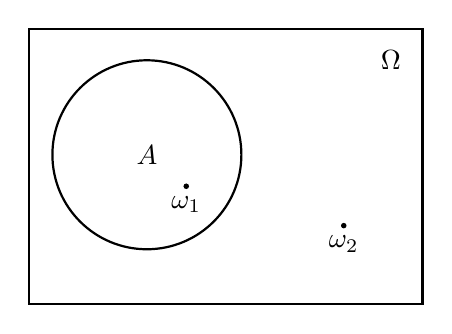
\begin{tikzpicture}[thick]
  \draw (0,0) rectangle (5,3.5);
  \draw (1.5,1.9)node{$A$} circle (1.2);
  \fill (2,1.5) circle(1pt) node[below] {$\omega_1$};
  \fill (4,1) circle(1pt) node[below] {$\omega_2$};
  \node at (4.6,3.1) {$\Omega$};
\end{tikzpicture}
\caption{维恩图\label{fig1.1.1}}
\end{figure}

\begin{example}
  掷一颗骰子的样本空间为:
  $ \Omega = \{1,2,\dotsc,6\}$.

  事件 $A=$“出现 1 点”,
  它由 $\Omega$ 的单个样本点“1”组成.

  事件 $B=$“出现偶数点”,
  它由 $\Omega$ 的三个样本点“2,4,6”组成.

  事件 $C=$“出现的点数小于7”,
  它由的全部样本点“1,2,3,4,5,6”组成,
  即必然事件$\Omega$.

  事件 $D=$“出现的点数大于6”,
  $\Omega$ 中任一样本点都不在 $D$ 中,
  所以 $D$ 是空集,
  即不可能事件 $\emptyset$.
\end{example}

\subsection{随机变量}

用来表示随机现象结果的变量称为\textbf{随机变量}\index{S!随机变量},
常用大写字母 $X$, $Y$, $Z$表示.
很多事件都可用随机变量表示,
表示时应写明随机变量的含义.

\begin{example}
  掷一颗骰子,
  出现的点数是一个随机变量,
  记为 $X$.
  则事件“出现3点”可用“$X = 3$”表示,
  事件“出现的点数不小于3”可用“$X \ge 3$”表示.
  又如“$X < 3$”表示事件“出现点数小于3”.

  掷两颗骰子的样本空间为
  \[
    \Omega =
    \left\{\begin{matrix}
      (1,1) & (1,2) & \dots & (1,6)\\
      (2,1) & (2,2) & \dots & (2,6)\\
      \dots & \dots & \dots & \dots\\
      (6,1) & (6,2) & \dots & (6,6)\\
    \end{matrix}\right\}
  \]
  $\Omega$ 共有 36 个样本点,
  若记 $X$ 与 $Y$ 分别为第一与第二颗骰子出现的点数,
  则 $X$ 与 $Y$ 均可取值:
  1,2,3,4,5,6.
  而事件“点数之和等于5”可表示成
  \[
    “X + Y = 5” = \{(1,4), (2,3), (3,2), (4,1)\}.
  \]

  另外事件“$\max (X,Y) =6$”表示事件“最大点数为6”,
  它含有
  \[
    (1,6),(6,1),(2,6),(6,2),(3,6),(6,3),(4,6),(6,4),(5,6),(6,5),(6,6)
  \]
  共 11 个样本点.
\end{example}

\begin{example}
  检查 10 件产品,
  其中不合格品数 $X$ 是一个随机变量,
  它可以取值 $0,1,\dotsc,10$.
  则事件“不合格品数不多于 1 件”可用“$X \le 1$”来表示. 而“$X>2$”表示事件“不合格品数超过2件”.
\end{example}

\begin{example}
  电视机的寿命 $T$ 是一个随机变量,
  则事件“寿命超过 \SI{40000}{\hour}”可用“$T>40000$”表示,
  而“$T \ge 10000$”表示事件”寿命不超过 \SI{10000}{\hour}”.
\end{example}

在不少场合,
用随机变量表示事件较为简洁明了.
这样一来,
事件有三种表示法:
\begin{enumerate}
  \item 用集合表示.
  \item 用语言表示,
  但语言要明白无误.
  \item 用随机变量表示.
\end{enumerate}
在实际问题中,
哪一种表示法方便就用哪一种.

\subsection{事件间的关系}

下而的讨论总是假设在同一个样本空间 $\Omega$ (即同一个随机现象) 中进行.
事件间的关系与集合间关系一样主要有以下几种:

\subsubsection{包含关系}

如果属于 $A$ 的样本点必属于 $B$,
则称 $A$ 被包含在 $B$ 中 (见图 \ref{fig1.1.2}),
或称 $B$ 包含 $A$,
记为 $A \subset B$,
或 $B \supset A$.
用概率论的语言说:
事件 $A$ 发生必然导致事件 $B$ 发生.

\begin{figure}[!ht]
  \centering
  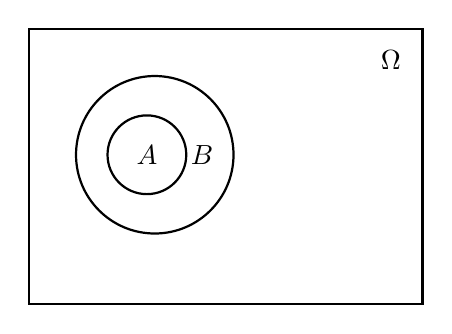
\begin{tikzpicture}[thick]
    \draw (0,0) rectangle (5,3.5);
    \draw (1.5,1.9)node{$A$} circle (0.5);
    \draw (1.6,1.9) circle (1.0);
    \node at (2.2,1.9) {$B$};
    \node at (4.6,3.1) {$\Omega$};
  \end{tikzpicture}
  \caption{$A \subset B$}\label{fig1.1.2}
\end{figure}

譬如掷一颗骰子,
事件 $A=$“出现4点”的发生必然导致事件 $B=$“出现偶数点”的发生,
故 $ A \subset B$.

又如电视机的寿命 $T$ 超过 \SI{10000}{\hour} (记为事件 $A = \{T>10000\}$) 和 $T$ 超过 \SI{20000}{\hour} (记为事件 $B = \{T>20000\}$),
则 $A \supset B$,
见图 \ref{fig1.1.3}.

\begin{figure}[!ht]
  \centering
\begin{tikzpicture}[thick]
  \draw[-Stealth](-1,0) -- (4,0) node[below] {$t$};
  \fill (0,0) node[below] {$0$} circle(1pt);
  \draw (1,0) [bend left=30] to node[above] {$A$} (3.5,1.2);
  \draw (2,0) [bend left=30] to node[below] {$B$} (3.6,0.7);
  \foreach \x in {1,2}
    \draw[fill=white] (\x,0) node[below] {$\x0000$} circle(1pt);
\end{tikzpicture}
  \caption{$\{ T > 10000 \} \supset \{ T > 20000 \}$}\label{fig1.1.3}
\end{figure}

对任一事件 $A$,
必有 $ \emptyset \subset A \subset \Omega $.

\subsubsection{相等关系}

如果事件 $A$ 与事件 $B$ 满足:
属于 $A$ 的样本点必属于 $B$,
而且属于 $B$ 的样本点必属于 $A$,
即 $ A \subset B $ 且 $ B \subset A$,
则称事件 $A$ 与 $B$ 相等,
记为 $A=B$.

从集合论观点看,
两个事件相等就意味着这两事件是同一个集合.
下例说明:
有时不同语言描述的事件也可能是同一件事.

\begin{example}
  \begin{enumerate}
    \item 掷两颗骰子,
    以 $A$ 记事件“两颗骰于的点数之和为奇数”,
    以 $B$ 记事件“两颗骰子的点数为一奇一偶”.
    很容易证明:
    $A$ 发生必然导致 $B$ 发生,
    而且 $B$ 发生也必然导致 $A$ 发生,
    所以 $A=B$.
    \item 口袋中有 $a$ 只黑球,
    $b$ 只白球 ($a$ 与 $b$ 都大于零),
    从中不返回地一只一只摸球.
    以 $A$ 记事件“最后摸出的几个球全是黑球”,
    以 $B$ 记事件“最后摸出的一只球是黑球”.
    对于此题粗看好像是 $A \ne B$,
    但只要设想将球全部摸完为止,
    则明显有:
    $A$ 发生必然会导致 $B$ 发生,
    即 $ A \subset B $;
    反之注意到事件 $A$ 中所述的“几个”最少是1只,
    也可以是2只,
    $\cdots$,
    最多为 $a$ 只,
    则 $B$ 发生时 $A$ 也必然会发生 (对于这点请读者仔细体会),
    即 $B \subset A$,
    由此得 $A=B$.
  \end{enumerate}
\end{example}

\subsubsection{互不相容}

如果 $A$ 与 $B$ 没有相同的样本点 (见图 \ref{fig1.1.4}),
则称 $A$ 与 $B$ 互不相容.
用概率论的语言说:
$A$ 与 $B$ 互不相容就是事件 $A$ 与事件 $B$ 不可能同时发生.

\begin{figure}[!ht]
  \centering
  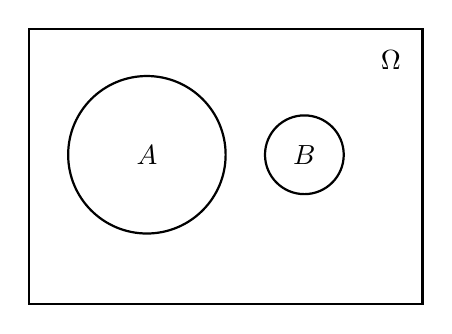
\begin{tikzpicture}[thick]
    \draw (0,0) rectangle (5,3.5);
    \draw (1.5,1.9)node{$A$} circle (1.0);
    \draw (3.5,1.9)node{$B$} circle (0.5);
    \node at (4.6,3.1) {$\Omega$};
  \end{tikzpicture}
  \caption{$A$ 与 $B$ 互不相容}\label{fig1.1.4}
\end{figure}

如在电视机寿命试验中,
“寿命小于1万小时”与“寿命大于5万小时”是两个互不相容的事件,
因为它们不可能同时发生.

\subsection{事件运算}

事件的运算与集合的运算相当,
有并、交、差和余等四种运算.

\subsubsection{事件 $A$ 与 $B$ 的并}
记为 $A \cup B$.
其含义为“由事件 $A$ 与 $B$ 中所有的样本点 (相同的只计入一次) 组成的新事件”(见 图 \ref{fig1.1.5}).
或用概率论的语言说:
“事件 $A$ 与 $B$ 中至少有一个发生”.

\begin{figure}[!ht]
  \centering
  \begin{tikzpicture}[thick]
    \draw (0,0) rectangle (5,3.5);
    \fill[pattern=north west lines]
      (1.5,1.9) circle (1) (2.8,1.9) circle(0.8);
    \draw (1.5,1.9)node[inner sep=0pt,fill=white]{$A$} circle (1);
    \draw (2.8,1.9)node[inner sep=0pt,fill=white]{$B$} circle(0.8);
    \node at (4.6,3.1) {$\Omega$};
  \end{tikzpicture}
  \caption{$A$ 与 $B$ 的并}\label{fig1.1.5}
\end{figure}

如在掷一颗骰子的试验中,
记事件 $A=$“出现奇数点”$=\{1,3,5\}$,
记事件 $B=$“出现的点数不超过3”$=\{1,2,3\}$,
则 $A$ 与 $B$ 的并为 $A \cup B = \{1,2,3,5\}$.

\subsubsection{事件 $A$ 与 $B$ 的交}

记为 $A \cap B$,
或简记为 $AB$.
其含义为“由事件 $A$ 与 $B$ 中公共的样本点组成的新事件”(见图 \ref{fig1.1.6})).
或用概率论的语言说:
“事件 $A$ 与 $B$ 同时发生”.

\begin{figure}[!ht]
  \centering
  \begin{tikzpicture}[thick]
    \draw (0,0) rectangle (5,3.5);
    \begin{scope}
    \clip(1.5,1.9) circle (1);
    \fill[pattern=north west lines] (2.8,1.9) circle(0.8);
    \end{scope}
    \draw (2.8,1.9) circle(0.8);
    \draw (1.5,1.9)node{$A$} circle (1);
    \draw (2.8,1.9)node{$B$} circle(0.8);
    \node at (4.6,3.1) {$\Omega$};
  \end{tikzpicture}
  \caption{$A$ 与 $B$ 的交}\label{fig1.1.6}
\end{figure}

如在掷一颗骰子的试验中,
记事件 $A=$“出现奇数点”$=\{1,3,5\}$,
记事件 $B=$“出现的点数不超过3”$=\{1,2,3\}$,
则 $A$ 与 $B$ 的交为 $AB = \{1,3\}$.

若事件 $A$ 与 $B$ 为互不相容,
则其交必为不可能事件,
即 $AB = \emptyset$,
反之亦然.
这表明:
$AB = \emptyset$ 就意味着 $A$ 与 $B$ 是互不相容事件.

事件的并与交运算可推广到有限个或可列个事件,
譬如有事件 $A_1$, $A_2$, $\dotsc$,
则 $\bigcup_{i=1}^n A_i$ 称为有限并;
$\bigcup_{i=1}^{+\infty} A_i$ 称为可列并;
$\bigcap_{i=1}^n A_i$ 称为有限交;
$\bigcup_{i=1}^{+\infty} A_i$ 称为可列交.

\subsubsection{事件 $A$ 对 $B$ 的差}

记为 $A-B$,
其含义为“由事件 $A$ 中而不在 $B$ 中的样本点组成的新事件”(见图 \ref{fig1.1.7}).
或用概率论的语言说:
“事件 $A$ 发生而 $B$ 不发生”.

\begin{figure}[!ht]
  \centering
  \begin{subfigure}{0.4\linewidth}
    \centering
    \begin{tikzpicture}[thick]
    \draw (0,0) rectangle (5,3.5);
    \fill[pattern=north west lines](1.5,1.9) circle (1);
    \filldraw[fill=white,draw=black] (2.8,1.9)node{$B$} circle(0.8);
    \draw (1.5,1.9)node[inner sep=0pt,fill=white]{$A$} circle (1);
    \node at (4.6,3.1) {$\Omega$};
  \end{tikzpicture}
    \caption{$A-B$}
  \end{subfigure}
  \begin{subfigure}{0.4\linewidth}
    \centering
    \begin{tikzpicture}[thick]
    \draw (0,0) rectangle (5,3.5);
    \filldraw[pattern=north west lines,draw=black](2,1.9)node
    [fill=white,inner sep=0pt]{$A$} circle (1);
    \filldraw[fill=white,draw=black] (1.5,1.9)node{$B$} circle(0.3);
    \node at (4.6,3.1) {$\Omega$};
  \end{tikzpicture}
    \caption{$A-B(A \supset B)$}
  \end{subfigure}
  \caption{}\label{fig1.1.7}
\end{figure}

如在掷一颗骰子的试验中,
记事件 $A=$“出现奇数点”$=\{1,3,5\}$,
记事件 $B=$“出现的点数不超过3”$=\{1,2,3\}$,
则 $A$ 对 $B$ 的差为 $A-B=\{15\}$.

若设 $X$ 为随机变量,
则有
\[
  \{ X = a \}
  = \{ X \le a \} - \{ X < a \},
  \quad
  \{ a < X \le b \}
  = \{ X \le b \} - \{ X \le a \}.
\]

\subsubsection{对立事件}

事件 $A$ 的对立事件,
记为 $\overline{A}$,
即“由在 $\Omega$ 中而不在 $A$ 中的样本点组成的新事件”(见图 \ref{fig1.1.8}),
或用概率论的语言说:
“$A$ 不发生”,
即 $\overline{A} = \Omega - A$.
注意,
对立事件是相互的,
即 $A$ 的对立事件是 $\overline{A}$,
而 $\overline{A}$ 的对立事件是 $A$,
即 $\overline{\overline{A}}=A$.
必然事件 $\Omega$ 与不可能事件 $\emptyset$ 互为对立事件,
即 $\overline{\Omega} = \emptyset$,
$\overline{\emptyset} = \Omega$.

\begin{figure}[!ht]
  \centering
  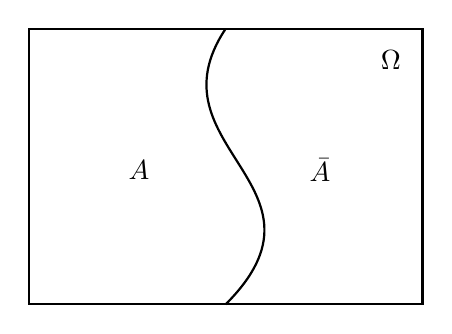
\begin{tikzpicture}[thick]
    \draw (0,0) rectangle (5,3.5);
    \node at (4.6,3.1) {$\Omega$};
    \draw (2.5,0).. controls (4,1.5) and (1.5,2)..(2.5,3.5);
    \draw (1.4,1.7)node{$A$} (3.7,1.7)node{$\bar A$};
  \end{tikzpicture}
  \caption{$A$ 的对立事件 $\overline{A}$}\label{fig1.1.8}
\end{figure}

如在掷一颗骰子的试验中,
事件 $A=$“出现奇数点”$= \{1,3,5\}$ 的对立事件是 $\overline{A} = \{2,4,6\}$,
事件 $B=$“出现的点数不超过3”$= \{1,2,3\}$ 的对立事件是 $\bar B =
\{4,5,6\}$.

$A$ 与 $B$ 互为对立事件的充要条件是:
$A \cap B = \emptyset$,
且 $A \cup B = \Omega$.

此性质也可作为对立事件的另一种定义,
即如果事件 $A$ 与 $B$ 满足:
$A \cap B = \emptyset$,
且 $A \cup B = \Omega$,
则称 $A$ 与 $B$ 互为对立事件,
记为 $\overline{A} = B$,
$\overline{B} = A$.

\begin{example}
  从数字$ 1, 2,\cdots, 9$ 中可重复地任取 $n$ 次 ($n \ge 2$),
  以 $A$ 表示事件“所取的 $n$ 个数字的乘积能被10整除”.
  因为乘积能被 10 整除必须既取到数字 5,
  又要取到偶数.
  所以 $A$ 的对立事件 $\overline{A}$ 为“所取的 $n$ 个数字中或者没有 5,
  或者没有偶数”.
  如果记 $B=$“所取的 $n$ 个数字中没有5”,
  $C=$“所取的 $n$ 个数字中没有偶数”,
  则 $\overline{A} = B \cup C$.
\end{example}

\begin{example}
  设 $A$、$B$、$C$ 是某个随机现象的三个事件,
  则
  \begin{enumerate}
    \item 事件“$A$ 与 $B$ 发生,
    $C$ 不发生”可表示为: $AB\overline{C}$.
    \item 事件“$A$、$B$、$C$ 中至少有一个发生”可表示为: $A \cup B \cup C$.
    \item 事件“$A$、$B$、$C$ 中至少有两个发生”可表示为: $AB \cup AC \cup BC$.
    \item 事件“$A$、$B$、$C$ 中恰好有两个发生”可表示为: $AB\overline{C} \cup A\overline{B}C \cup \overline{A}BC$.
    \item 事件“$A$、$B$、$C$ 同时发生”可表示为: $ABC$.
    \item 事件“$A$、$B$、$C$ 都不发生”可表示为: $\overline{A}\overline{B}\overline{C}$.
    \item 事件“$A$、$B$、$C$ 不全发生”可表示为: $\overline{A} \cup \overline{B} \cup \overline{C}$.
  \end{enumerate}
\end{example}

\subsubsection{事件的运算性质}
\begin{enumerate}
  \item 交换律
  \begin{equation}\label{eq1.1.1}
    A \cup B = B \cup A, \quad AB = BA
  \end{equation}
  \item 结合律
  \begin{gather}
    (A \cup B) \cup C = A \cup (B \cup C),\label{eq1.1.2}\\
    (AB)C = A(BC).\label{eq:1.1.3}
  \end{gather}
  \item 分配律
  \begin{gather}
    (A \cup B) \cap C = AC \cup BC,\label{eq1.1.4}\\
    (A \cap B) \cup C = (A \cup C) \cap (B \cup C).\label{eq1.1.5}
  \end{gather}
  \item 对偶律 (德莫根公式)
  \begin{gather}
    \text{事件并的对立等于对立的交:} \quad \overline{A \cup B} = \overline{A} \cap \overline{B},\label{eq1.1.6}\\
    \text{事件交的对立等于对立的并:} \quad \overline{A \cap B} = \overline{A} \cup \overline{B}.\label{eq1.1.7}
  \end{gather}
\end{enumerate}

事件运算的对偶律是很有用的公式.
这些性质是不难证明的,
在此我们用集合论的语言证明其中的 \eqref{eq1.1.6} 式.

\subsubsection*{\eqref{eq1.1.6} 式的证明}

设 $\omega \in \overline{A \cup B}$,
即 $\omega \notin A \cup B$,
这表明 $\omega$ 既不属于 $A$,
也不属于 $B$,
这意味着 $\omega \notin A$ 和 $\omega \notin B$ 同时成立,
所以 $\omega \in \overline{A}$ 与 $\omega \in \overline{B}$ 同时成立,
于是有 $\omega \in \overline{A} \cap \overline{B}$,
这说明
\[
  \overline{A \cup B} \subset \overline{A} \cap \overline{B}.
\]

反之,
设 $\omega \in \overline{A} \cap \overline{B}$,
即同时有 $\omega \in \overline{A}$ 和$\omega \in \overline{B}$,
从而同时有 $\omega \notin A$ 和 $\omega \notin B$,
这意味着 $\omega$ 不属于 $A$ 与 $B$ 中的任一个,
即 $\omega \notin A \cup B$,
也就是有 $\omega \in \overline{A \cup B}$,
这说明
\[
  \overline{A \cup B} \supset \overline{A} \cap \overline{B}.
\]

综合上述两方面,
可得
\[
  \overline{A \cup B} = \overline{A} \cap \overline{B}.
\]
\eqref{eq1.1.6} 式得证.

德莫根公式可推广到多个事件及可列个事件场合:
\begin{gather}
  \overline{\bigcup _{i=1} ^n A _i} = \bigcap _{i=1} ^n \overline{A} _i;
  \quad \overline{\bigcup _{i=1} ^{+\infty} A _i} = \bigcap _{i=1} ^{+\infty} \overline{A} _i; \label{eq1.1.8}\\
  \overline{\bigcap _{i=1} ^n A _i} = \bigcup _{i=1} ^n \overline{A} _i;
  \quad \overline{\bigcap _{i=1} ^{+\infty} A _i} = \bigcup _{i=1} ^{+\infty} \overline{A} _i. \label{eq1.1.9}
\end{gather}

\subsection{事件域}

在此我们要给出的“事件域”概念,
目的是为下一节定义事件的概率作准备.

所谓的“事件域”从直观上讲就是一个样本空间中某些子集组成的集合类,
以后记事件域为 $\mathscr{F}$.

当样本空间是实数轴上的一个区间时,
可以人为地构造出无法测量其长度的子集,
这样的子集常被称为不可测集.
如果将这些不可测集也看成是事件,
那么这些事件将无概率可言,
这是我们不希望出现的现象,
为了避兔这种现象出现,
我们没有必要将连续样本空间的所有子集都看成是事件,
只需将我们感兴趣的子集 (又称\textbf{可测集})\index{K!可测集} 看成是事件即可.

现在的问题是:
我们应该对哪些子集感兴趣,
或换句话说,
$\mathscr{F}$ 中应该有哪些元素?
首先 $\mathscr{F}$ 应该包括 $\Omega$ 和 $\emptyset$;
其次应该保证事件经过前面所定义的各种运算 (并、交、差、对立) 后仍然是事件,
即 $\mathscr{F}$ 要对集合的运算有封闭性.
经过研究人们发现
\begin{itemize}
  \item 交的运算可通过并与对立来实现 (德莫根公式).
  \item 差的运算可通过对立与交来实现 ($A - B = A\overline{B}$).
\end{itemize}

这样一来,
可给出事件域的定义如下.


\begin{definition}{}{1.1.1}
  设 $ \Omega $ 为一样本空间,
  $\mathscr{F}$ 为 $\Omega$ 的某些子集所组成的集合类,
  如果 $\mathscr{F}$ 满足:
  \begin{enumerate}
      \item $\Omega \in \mathscr{F}$;
      \item 若 $A \in \mathscr{F}$, 则对立事件 $\overline{A} \in \mathscr{F}$;
      \item 若 $A _n \in \mathscr{F}$, $1,2,\dotsc$, 则可列并 $\bigcup _{n=1} ^{+\infty} A _n \in \mathscr{F}$.
  \end{enumerate}
  则称 $\mathscr{F}$ 为一个\textbf{事件域}, \index{S!随机事件!事件域}
  又称为 \textbf{$\sigma$ 代数}. \index{S!随机事件!$\sigma$代数}
\end{definition}

在概率论中,
又称 $(\Omega, \mathscr{F})$ 为\textbf{可测空间},\index{S!随机事件!可测空间}
这里“可测”是指 $\mathscr{F}$ 中都是有概率可言的事件.

\begin{example}
  常见的事件域
  \begin{enumerate}
    \item 若样本空间只含两个样本点: $\Omega = \{\omega_1, \omega_2\}$, 记 $A = \{\omega_1\}$, $\overline{A} = \{\omega_2\}$, 则其事件域为 $\mathscr{F} = \{\emptyset, A, \overline{A}, \Omega\}$.
    \item 若样本空间含有 $n$ 个样本点: $\Omega = \{\omega_1, \omega_2, \dotsc, \omega_n\}$, 则其事件域 $\mathscr{F}$ 是由空集 $\emptyset$、$n$ 个单元素集、$\binom{n}{2}$ 个双元素集、$\binom{n}{3}$ 个三元素集……和 $\Omega$ 组成的集合类, 这时 $\mathscr{F}$ 中共有 $\binom{n}{0} + \binom{n}{1} + \binom{n}{2} + \dotsb + \binom{n}{n} = 2^n$ 个事件.
    \item 若样本空间含有可列个样本点: $\Omega = \{\omega_1, \omega_2, \dotsc, \omega_n, \dotsc\}$, 则其事件域 $\mathscr{F}$ 是由空集 $\emptyset$、可列个单元素集、可列个双元素集……可列个 $n$ 个元素集……和 $\Omega$ 组成的集合类, 这时 $\mathscr{F}$ 是由可列个的可列个 (仍为可列个) 元素 (事件) 组成.
    \item 若样本空间含有全体实数: $\Omega = (-\infty, +\infty) = \mathbb{R}$. 这时事件域 $\mathscr{F}$ 中的元素无法一一列出, 而是由一个基本集合类逐步扩展形成, 具体操作如下:
    \begin{itemize}
      \item 取基本集合类 $\mathscr{F} =$“全体半直线组成的类”, 即
      \[ \mathscr{F} = \{(-\infty, x); -\infty < x < +\infty\}.\]
      \item 利用事件域的要求, 首先把有限的左闭右开区间扩展进来:
      \[ [a, b) = (-\infty, b) - (\infty, a), \quad \text{其中 } a, b \text{ 为任意实数}. \]
      \item 再把闭区间、单点集、左开右闭区间、开区间扩展进来:
      \[ [a,b] = \bigcap _{n=1} ^{+\infty} [a, b + 1/n), \]
      \[ \{b\} = [a, b] - [a, b), \]
      \[ (a, b] = [a, b] - \{a\}, \]
      \[ (a, b) = [a, b) - \{a\}. \]
      \item 最后用 (有限个或可列个) 并运算和交运算把实数集中一切有限集、可列集、开集、闭集都扩展进来.
    \end{itemize}

    经过上述几步扩展所得之集的全体就是人们希望得到的事件域 $\mathscr{F}$,
    因为它满足事件城的定义.
    这样的事件域 $\mathscr{F}$ 又称为\textbf{波雷尔 (Borel) 事件城},\index{S!随机事件!波雷尔 事件域}
    域中的每个元素 (集合)又称为波雷尔集,
    或称为可测集,
    这种可测集都是有概率可言的事件.
  \end{enumerate}
\end{example}

\begin{xiti}
  \item 写出下列随机试验的样本空间:
  \begin{enumerate}
    \item 抛三枚硬币;
    \item 抛三颗骰子;
    \item 连续抛一枚硬币, 直至出现正为之;
    \item 在某十字路口, 一小时内通过的机动车辆数;
    \item 某城市一天内的用电量.
  \end{enumerate}

  \item 在抛三枚硬币的试验中写出下列事件的集合表示:
  \begin{itemize}
    \item $A =$“至少出现一个正面”;
    \item $B =$“最多出现一个正面”;
    \item $C =$“恰好出现一个正面”;
    \item $D =$“出现三面相同”.
  \end{itemize}

  \item 设 $A$、$B$、$C$ 为三事件, 试表示下列事件:
  \begin{enumerate}
    \item $A$、$B$、$C$ 都发生或都不发生;
    \item $A$、$B$、$C$ 中不多于一个发生;
    \item $A$、$B$、$C$ 中不多于两个发生;
    \item $A$、$B$、$C$ 中至少有两个发生.
  \end{enumerate}

  \item 请指明以下事件 $A$ 和 $B$ 间的关系:
  \begin{enumerate}
    \item 检查两件产品, 记事件 $A =$“至少有一件不合格产品”, $B =$“两次检查结果不同”.
    \item 设 $T$ 表示轴承寿命, 记事件 $A = \{T > \text{\SI{5000}{\hour}}\}$, $B = \{T > \text{\SI{8000}{\hour}}\}$.
  \end{enumerate}

  \item 设 $X$ 为随机变量, 其样本空间为 $\Omega = \{0 \le T \le 2\}$, 记事件 $A =\{0.5 < X \le 1\}$, $B = \{0.25 \le X < 1.5\}$. 写出下列事件:
  \begin{enumerate}
    \item $\overline{A}B$,
    \item $\overline{A} \cup B$,
    \item $\overline{AB}$,
    \item $\overline{A \cup B}$.
  \end{enumerate}

  \item 对飞机进行两次射击, 每次射一弹, 设 $A = \{$恰有一弹击中飞机$\}$, $B = \{$至少有弹击中飞机$\}$, $C = \{$两弹都击中飞机$\}$, $D = \{$两弹都没击中飞机$\}$. 又设随机变量 $X$ 为击中飞机的次数, 试用 $X$ 表示事件 $A$, $B$, $C$, $D$. 进一步问 $A$, $B$, $C$, $D$ 中哪些是互不相容的事件? 哪些是对立的事件?

  \item 试问下列命题是否成立?
  \begin{enumerate}
    \item $ A - (B - C) = (A - B) \cup C.$
    \item 若 $AB = \emptyset$ 且 $ C \subset A$, 则 $BC = \emptyset$.
    \item $(A \cup B) - B = A$.
    \item $(A - B) \cup B = A$.
  \end{enumerate}

  \item 试用维恩图说明, 当事件 $A$ 与 $B$ 互不相容时, 能否得出结论 $\overline{A}$ 与 $\overline{B}$ 相容.

  \item 请叙述下列事件的对立事件:
  \begin{enumerate}
    \item $A = $“掷两枚硬币, 皆为正面”;
    \item $B = $“射击三次, 皆命中目标”;
    \item $C = $“加工四个零件, 至少有一个合格品”.
  \end{enumerate}

  \item 如果 $A$ 与 $B$ 互为对立事件, 证明: $\overline{A}$ 与 $\overline{B}$ 也互为对立事件.

  \item 设 $\mathscr{F}$ 为一事件域, 若 $A_n \in \mathscr{F}$, $n = 1,2, \dotsc$, 试证:
  \begin{enumerate}
    \item $\emptyset \in \mathscr{F}$;
    \item 有限并 $\bigcup _{i=1}^n A_i \in \mathscr{F}$, $n \ge 1$;
    \item 有限交 $\bigcap _{i=1}^n A_i \in \mathscr{F}$, $n \ge 1$;
    \item 可列交 $\bigcap _{i=1}^{+\infty} A_i \in \mathscr{F}$;
    \item 差运算 $A_1 - A_2 \in \mathscr{F}$.
  \end{enumerate}
\end{xiti}

\section{概率的定义及其确定方法}

在这一节中,
我们要给出概率的定义及其确定方法,
这是概率论中最基本的个问题.
简单而直观的说法就是:
概率是随机事件发生的可能性大小,
对此我们先看下面一些经验事实:
\begin{enumerate}
  \item 随机事件的发生是带有偶然性.
  但随机事件发生的可能性是有大小之分的,
  例如口袋中有10只相同大小的球,
  其中9只黑球,
  1只红球,
  从口袋中任取1球,
  人们的共识是:
  取出黑球的可能性比取出红球的可能性大;
  \item 随机事件发生的可能性是可以设法度量的,
  就好比一根木棒有长度,
  一块土地有面积一样.
  例如抛一枚硬币,
  出现正面与出现反面的可能性是相同的,
  各为 $1/2$.
  足球裁判就用抛硬币的方法让双方队长选择场地,
  以示机会均等;
  \item 在日常生活中,
  人们对一些随机事件发生的可能性大小往往是用百分比 (0到1之间的一个数) 进行度量的.
  例如购买彩券后可能中奖,
  可能不中奖,
  但中奖的可能性大小可以用中奖率来度量;
  抽取一个产品可能为合格品,
  也可能为不合格品,
  但产品质量的好坏可以用不合格品率来度量;
  新生要儿可能为男孩,
  也可能为女孩,
  但生男孩的可能性可以用男婴出生率来度量.
\end{enumerate}

在概率论发展的历史上,
曾有过概率的古典定义、概率的几何定义、概率的频率定义和概率的主观定义.
这些定义各适合一类随机现象,
那么如何给出适合一切随机现象的概率的最一般的定义呢?
1900年数学家希尔伯特 (1862-1943) 提出要建立概率的公理化定义以解决这个问题,
即以最少的几条本质特性出发去刻画概率的概念.
1933年前苏联数学家柯尔莫哥洛夫 (1903-1987) 首次提出了概率的公理化定义,
这个定义既概括了历史上几种概率定义中的共同特性,
又避免了各自的局限性和含混之处,
不管什么随机现象,
只有满足定义中的三条公理,
才能说它是概率.
这一公理化体系迅速获得举世公认,
是概率论发展史上的一个里程碑.
有了这个公理化定义后,
概率论得到了很快的发展.

\subsection{概率的公理化定义}

\begin{definition}{}{1.2.1}
  设 $\Omega$ 为一个样本空间,
  $\mathscr{F}$ 为 $\Omega$ 的某些子集组成的一个事件域.
  如果对任一事件 $A \in \mathscr{F}$,
  定义在 $\mathscr{F}$ 上的一个实值函数 $P(A)$ 满足:
  \begin{enumerate}
    \item 非负性公理:
    若 $A \in \mathscr{F}$,
    则 $P(A) \ge 0$;
    \item 正则性公理:
    $P (\Omega) = 1$;
    \item 可列可加性公理:
    若 $A_1$, $A_2$, \dots, $A_n$, \dots, 互不相容,
    有
    \begin{equation}
      P \biggl( \bigcup _{i=1} ^{+\infty} A_i \biggr) = \sum _{i=1} ^{+\infty} P ( A _i ),\label{eq1.2.1}
    \end{equation}
  \end{enumerate}
  则称 $P (A)$ 为事件 $A$ 的概率,
  称三元素 $(\Omega, \mathscr{F}, \mathscr{P})$ 为\textbf{概率空间}.
\end{definition}

概率的公理化定义刻画了概率的本质,
概率是集合 (事件) 的函数,
若在事件域 $\mathscr{F}$ 上给出一个函数,
当这个函数能满足上述三条公理,
就被称为概率;
当这个函数不能满足上述三条公理中任一条,
就被认为不是概率.

公理化定义没有告诉人们如何去确定概率.
历史上在公理化定义出现之前概率的频率定义、古典定义、几何定义和主观定义都在一定的场合下,
有着各自确定概率的方法,
所以在有了概率的公理化定义之后,
把它们看作确定概率的方法是恰当的.
下面先介绍在确定概率的古典方法中大量使用的排列与组合公式,
然后分别讲述确定概率的方法.

\subsection{排列与组合公式}

排列与组合都是计算“从 $n$ 个元素中任取 $r$ 个元素”的取法总数公式,
其主要区别在于:
如果不讲究取出元素间的次序,
则用组合公式,
否则用排列公式;
而所谓讲究元素间的次序,
可以从实际问题中得以辨别,
例如两个人相互握手是不讲次序的,
而两个人排队是讲次序的,
因为“甲右乙左”与“乙右甲左”是两件事.

排列与组合公式的推导都基于如下两条计数原理:
\begin{enumerate}
  \item 乘法原理:
  如果某件事经 $k$ 个步骤才能完成,
  做第一步有 $m_1$ 种方法,
  做第二步有 $m_2$ 种方法,
  \dots,
  做第 $k$ 步有 $m_k$ 种方法.
  那么完成这件事共有 $m_1 \times m_2 \times \dotsb \m_k$ 种方法.

  譬如,
  甲城到乙城有3条旅游线路,
  由乙城到丙城有2条旅游线路,
  那么从甲城经乙城去丙城共有 $3 \times 2 = 6$ 条旅游线路.

  \item 加法原理:
  如果某件事可由 $k$ 类不同途径之一去完成,
  在第一类途径中有 $m_1$ 种完成方法,
  在第二类途径中有 $m_2$ 种完成方法,
  \dots,
  在第 $k$ 类途径中有 $m_k$ 种完成方法,
  那么完成这件事共有 $m_1 + m_2 + \dotsb + m_k$ 种方法.

  譬如,
  由甲城到乙城去旅游有三类交通工具:
  汽车、火车和飞机.
  而汽车有5个班次,
  火车有3个班次,
  飞机有2个班次,
  那么从甲城到乙城共有 $5 + 3 + 2 = 10$ 个班次供旅游者选择.
\end{enumerate}

排列与组合的定义及其计算公式如下.
\begin{enumerate}
  \item 排列:
  从 $n$ 个不同元素中任取 $r (r \le n)$ 个元素排成一列 (考虑元素先后出现次序),
  称此为一个排列,
  此种排列的总数记为 $P_n^r$,
  按乘法原理,
  取出的第一个元素有 $n$ 种取法,
  取出的第二个元素有 $n - 1$ 种取法\dots
  取出的第 $r$ 个元素有 $n - r + 1$ 种取法,
  所以有
  \begin{equation}
    P_n^r = n \times (n - 1) \times \dotsb \times (n - r + 1) = \frac{n!}{(n - r)!}.\label{eq1.2.2}
  \end{equation}
  若 $r = n$,
  则称为全排列,
  记为 $_n$.
  显然,
  全排列 $P_n = n!$.

  \item 重复排列:
  从 $n$ 个不同元素中每次取出一个,
  放回后再取下一个,
  如此连续取 $r$ 次所得的排列称为重复排列,
  此种重复排列数共有 $n^r$ 个.
  注意这里的 $r$ 允许大于 $n$.

  \item 组合:
  从 $n$ 个不同元素中任取 $r (r \le n)$ 个元素并成一组 (不考虑元素间的先后次序),
  称此为一个组合,
  此种组合的总数记为 $\binom{n}{r}$ 或 $C_n^r$.
  按乘法原理此种组合的总数为
  \begin{equation}
    \binom{n}{r} = \frac{P_n^r}{r!} = \frac{n (n - 1) \dotsb (n - r + 1)}{r!} = \frac{n!}{r! (n - r)!}.\label{eq1.2.3}
  \end{equation}
  在此规定 $0! = 1$ 与 $\binom{n}{0} = 1$.

  \item 重复组合:
  从 $n$ 个不同元素中每次取出一个,
  放回后再取下一个,
  如此连续取 $r$ 次所得的组合称为重复组合,
  此种重复组合总数为 $\binom{n + r - 1}{r}$.
  注意这里的 $r$ 也允许大于 $n$.
\end{enumerate}

上述四种排列组合及其总数计算公式,
在确定概率的古典方法中经常使用,
但在使用中要注意识别有序与无序、重复与不重复。

\subsection{确定概率的频率方法}

确定概率的频率方法是一种最常用的方法,
其基本思想是:
\begin{enumerate}
  \item 与考察事件 $A$ 有关的随机现象可大量重复进行.
  \item 在 $n$ 次重复试验中,
  记 $n (A)$ 为事件 $A$ 出现的次数,
  又称 $n (A)$为事件 $A$ 的\textbf{频数},
  称
  \begin{equation}
    f_n (A) = \frac{n (A)}{n}\label{eq1.2.4}
  \end{equation}
  为事件 $A$ 出现的\textbf{频率}.

  \item 人们的长期实践表明:
  随着试验重复次数 $n$ 的增加,
  频率 $f_n (A)$ 会稳定在某一常数 $a$ 附近.
  我们称这个常数为\textbf{频率的稳定值}.
  这个频率的稳定值就是我们所求的概率.

  \item 频率方法的缺点是:
  在现实世界里,
  人们无法把一个试验无限次地重复下去,
  因此要精确获得频率的稳定值是困难的.
  但频率方法提供了概率的一个可供想像的具体值,
  并且在试验重复次数 $n$ 较大时,
  可用频率给出概率的一个近似值,
  这一点是频率方法最有价值的地方.
  在统计学中就是如此做的,
  且称频率为概率的估计值.
\end{enumerate}

容易验证:
用频率方法确定的概率满足公理化定义,
它的非负性与正则性是显然的,
而可加性只需注意到:
当 $A$ 与 $B$ 互不相容时,
计算 $A \cup B$ 的频数可以分别计算的 $A$ 的频数和 $B$ 的频数,
然后再相加,
这意味着 $n (A \cup B) = n (A) + n (B)$.
从而有
\begin{align*}
  f _n (A \cup B) &= \frac{n (A \cup B)}{n} = \frac{n (A) + n (B)}{n}\\
  &= \frac{n (A)}{n} + \frac{n (B)}{n} = f _n (A) + f _n (B).
\end{align*}

\begin{example}
  说明频率稳定性的例子.
  \begin{enumerate}
    \item 抛硬币试验

    历史上有不少人做过抛硬币试验,
    其结果见表~\ref{tab1.2.1}.
    从表中的数据可以看出:
    出现正面的频率逐渐稳定在0.5,
    用频率的方法可以说:
    出现正面的概率为0.5.

    \begin{table}[h]
      \centering
      \caption{历史上抛硬币试验的若干结果}\label{tab1.2.1}
      \begin{tabularx}{0.9\linewidth}{*{4}{X}}
        \toprule
        实验者 & 抛硬币次数 & 出现正面次数 & 频率\\
        \midrule
        德莫根 (De morgan) & 2048 & 1061 & 0.5181\\
        蒲丰 (Buffon) & 4040 & 2048 & 0.5069\\
        费勒 (Feller) & 10000 & 4979 & 0.4979\\
        皮尔逊 (Pearson) & 12000 & 6019 & 0.5016\\
        皮尔逊 & 24000 & 12012 & 0.5005\\
        \bottomrule
      \end{tabularx}
    \end{table}

    \item 英语字母的频率

    人们在生活实践中已经认识到:
    英语中某些字母出现的频率要高于另外一些字母.
    但26个英文字母各自出现的频率到底是多少?
    有人对各类典型的英语书刊中字母出现的频率进行统计,
    发现各个字母的使用频率相当稳定 (见表~\ref{tab1.2.2}).
    这项研究对计算机键盘的设计 (在方便的地方安排使用频率最高的宇母键)、信息的编码 (用较短的码编排使用频率最高的字母键) 等等方面都是十分有用的.

    \begin{table}[h]
      \centering
      \caption{英文字母的使用率}\label{tab1.2.2}
      \begin{tabularx}{0.9\linewidth}{*{6}{Z}}
        \toprule
        字母 & 使用频率 & 字母 & 使用频率 & 字母 & 使用频率\\
        \midrule
        E & 0.1268 & L & 0.0394 & P & 0.0186\\
        T & 0.0978 & D & 0.0389 & B & 0.0156\\
        A & 0.0788 & U & 0.0280 & V & 0.0102\\
        O & 0.0776 & C & 0.0268 & K & 0.0060\\
        I & 0.0707 & F & 0.0256 & X & 0.0016\\
        N & 0.0706 & M & 0.0244 & J & 0.0010\\
        S & 0.0634 & W & 0.0214 & Q & 0.0009\\
        R & 0.0594 & Y & 0.0202 & Z & 0.0006\\
        H & 0.0573 & G & 0.0187 &   &       \\
        \bottomrule
      \end{tabularx}
    \end{table}

    \item 女婴出生频率

    研究女婴出生频率,
    对人口统计是很重要的.
    历史上较早研究这个问题的有拉普拉斯 (1794-1827),
    他对伦敦、彼得堡、柏林和全法国的大量人口资料进行研究,
    发现女要出生频率总是在 $21/43$ 左右波动.

    统计学家克拉梅 (1893-1985) 用瑞典 1935 年的官方统计资料 (见表~\ref{tab1.2.3}),
    发现女要出生频率总是在 0.482 左右波动.

    \begin{table}[h]
      \centering
      \caption{瑞典 1935 年各月出生女的频率}\label{tab1.2.3}
      \begin{tabularx}{0.9\linewidth}{*{8}{Z}}
        \toprule
        月份 & 1 & 2 & 3 & 4 & 5 & 6 & \\
        \midrule
        婴儿数 & 7280 & 6957 & 7883 & 7884 & 7892 & 7609 &\\
        女婴数 & 3537 & 3407 & 3866 & 3711 & 3775 & 3665 &\\
        频率 & 0.486 & 0.489 & 0.490 & 0.471 & 0.478 & 0.482 &\\
        \midrule
        \midrule
        月份 & 7 & 8 & 9 & 10 & 11 & 12 & 全年\\
        \midrule
        婴儿数 & 7585 & 7393 & 7203 & 6903 & 6552 & 7132 & 88273\\
        女婴数 & 3621 & 3596 & 3491 & 3391 & 3160 & 3371 & 42591\\
        频率 & 0.462 & 0.484 & 0.485 & 0.491 & 0.482 & 0.473 & 0.4825\\
        \bottomrule
      \end{tabularx}
    \end{table}
  \end{enumerate}
\end{example}

\subsection{确定概率的古典方法}

确定概率的古典方法是概率论历史上最先开始研究的情形.
它简单、直观,
不需要做大量重复试验,
而是在经验事实的基础上,
对被考察事件的可能性进行逻辑分析后得出该事件的概率.

古典方法的基本思想如下:
\begin{enumerate}
  \item 所涉及的随机现象只有有限个样本点,
  譬如为 $n$ 个.
  \item 每个样本点发生的可能性相等 (称为等可能性).
  例如,
  抛一枚均匀硬币,
  “出现正面”与“出现反面”的可能性相等;
  抛一枚均匀骰子,
  出现各点 (1--6) 的可能性相等;
  从一副扑克牌中任取一张,
  每张牌被取到的可能性相等.

  \item 若事件 $A$ 含有 $k$ 个样本点,
  则事件 $A$ 的概率为
  \begin{equation}
    P (A) = \frac{\text{事件 } A \text{ 所含样本点的个数}}{\Omega \text{ 中所有样本点的个数}}
    = \frac{k}{n}.\label{eq1.2.5}
  \end{equation}
\end{enumerate}

容易验证,
由上式确定的概率满足公理化定义,
它的非负性与正则性是显然的;
而满足可加性的理由与频率方法类似:
当 $A$ 与 $B$ 互不相容时,
计算 $A \cup B$ 的样本点个数可以分别计算 $A$ 的样本点个数和 $B$ 的样本点个数,
然后再相加,
从而有可加性 $P (A \cup B) = P (A) + P (B) $.

在古典方法中,
求事件 $A$ 的概率主要是计算 $A$ 中含有的样本点的个数和 $\Omega$ 中含有的样本点的个数.
所以在计算中经常用到排列组合工具.

\begin{example}
  掷两枚硬币,
  求出现一个正面一个反面的概率.
\end{example}

\begin{solution}
  此例的样本空间为 $\Omega = \{ (\text{正}, \text{正})$, $(\text{正}, \text{反})$, $(\text{反}, \text{正})$, $(\text{反}, \text{反}) \}$.
  所以 $\Omega$ 中含有样本点的个数为4,
  事件“出现一个正面一个反面”含有的样本点的个数为2个,
  因此所求概率为 1/2.
\end{solution}

注意,
如果将此样本空间记成 $\Omega = \{ (\text{二正})$, $(\text{二反})$, $(\text{一正一反}) \}$,
则此三个样本点不是等可能的.

在计算古典概型时,
一般不用把样本空间详细写出,
但一定要保证样本点为等可能.
以下是一些较为有用的模型,
请读者熟练掌握和灵活运用.

\begin{example}[抽样模型]\label{exmp1.2.3}
  一批产品共有 $N$ 个,
  其中 $M$ 个是不合格品,
  $N - M$个是合格品.
  从中随机取出 $n$ 个,
  试求事件 $A _m =$“取出的 $n$ 个产品中有 $m$ 个不合格品”的概率.
\end{example}

\begin{solution}
  先计算样本空间 $\Omega$ 中样本点的个数:
  从 $N$ 个产品中任取 $n$ 个,
  因为不讲次序,
  所以样本点的总数为 $\binom{N}{n}$.
  又因为是随机抽取的,
  所以这 $\binom{N}{n}$ 个样本点是等可能的.

  下面我们先计算事件 $A _0$, $A _1$ 的概率,
  然后再计算 $A _m$ 的概率.

  因为事件 $A _0 =$“取出的 $n$ 个产品中有 0 个不合格品”$=$“取出的 $n$ 个产品全是合格品”,
  这意味着取出的 $n$ 个产品全是从 $N - M$ 个合格品中抽取,
  所以有 $\binom{N - M}{n}$ 种取法,
  故 $A _0$ 的概率为
  \[
    P (A _0) = \frac{\binom{N - M}{n}}{\binom{N}{n}}.
  \]

  事件 $A _1 =$“取出的 $n$ 个产品中有 1 个不合格品”,
  要使取出的 $n$ 个产品中只有一个不合格品,
  其他 $n - 1$ 个是合格品,
  那么必须分两步进行:

  第一步:
  从 $M$ 个不合格品中随机取出1个,
  共有 $\binom{M}{1}$ 种取法.

  第二步:
  从 $N - M$ 个合格品中随机取出 $n - 1$ 个,
  共有 $\binom{N - M}{n - 1}$ 种取法.

  所以根据乘法原理,
  $A _1$ 中共有 $\binom{M}{1} \binom{N - M}{n - 1}$ 个样本点.
  故 $A _1$ 的概率为
  \[
    P (A _1) = \frac{\binom{M}{1} \binom{N - M}{n - 1}}{\binom{N}{n}}.
  \]

  有了以上对 $A _0$ 和 $A _1$ 的分析,
  我们就容易计算一般事件 $A _m$ 中含有的样本点个数:
  要使 $A _m$ 发生,
  必须从 $M$ 个不合格品中抽 $m$ 个,
  再从 $N - M$ 个合格品中抽 $n - m$ 个,
  根据乘法原理,
  $A _m$ 含有 $\binom{M}{m} \binom{N - M}{n - m}$ 个样本点,
  由此得 $A _m$ 的概率为
  \begin{equation}
    P (A _m) = \frac{\binom{M}{m} \binom{N - M}{n - m}}{\binom{N}{n}},
    \quad m = 0,1,2,\dotsc,r, \quad r = \min (n, M).\label{eq1.2.6}
  \end{equation}
  注意,
  在此应有 $m \le n$, $m \le M$.
  所以 $m \le \min(n,M)$,
  否则其概率为0.

  如果取 $N=9$,
  $M=3$,
  $n=4$,
  则有
  \begin{align*}
    & P (A _0) = \frac{\binom{6}{4}}{\binom{9}{4}} = \frac{5}{42}.\\
    & P (A _1) = \frac{\binom{6}{3}\binom{3}{1}}{\binom{9}{4}} = \frac{20}{42}.\\
    & P (A _2) = \frac{\binom{6}{2}\binom{3}{2}}{\binom{9}{4}} = \frac{15}{42}.\\
    & P (A _2) = \frac{\binom{6}{1}\binom{3}{3}}{\binom{9}{4}} = \frac{2}{42}.
  \end{align*}

  将以上计算结果列成表~\ref{tab1.2.4}.
  \begin{table}[h]
    \centering
    \caption{事件 $A_m$ 的概率}\label{tab1.2.4}
    \begin{tabularx}{0.9\linewidth}{*{5}{X}}
      \toprule
      $m$ & 0 & 1 & 2 & 3\\
      \midrule
      $P (A _m)$ & $\frac{5}{42}$ & $\frac{20}{42}$ & $\frac{15}{42}$ & $\frac{2}{42}$\\
      \bottomrule
    \end{tabularx}
  \end{table}
  由于表中概率之和为1,
  所以可称其为一个概率分布.
  若把 $m$ 看作随机变量,
  则此分布为 $m$ 的分布.
\end{solution}

\begin{example}[放回抽样]
  抽样有两种方式:
  不放回抽样与放回抽样.
  上例讨论的是不放回抽样,
  放回抽样是抽取一个后放回,
  然后再抽取下一个……
  如此重复直至抽出 $n$ 个为止.
  现对例~\ref{exmp1.2.3} 在有放回抽样情况下,
  讨论事件 $B _n=$“取出的 $n$ 个产品中有 $m$ 个不合格品”的概率.
\end{example}

\begin{solution}
  同样我们先计算样本空间 $\Omega$ 中样本点的个数:
  第一次抽取时,
  可从 $N$ 个中任取一个,
  有 $N$ 种取法.
  因为是放回抽取,
  所以第二次抽取时,
  仍有 $N$ 种取法……
  如此下去,
  每一次都有 $N$ 种取法,
  一共抽取了 $n$ 次,
  所以共有 $N ^n$ 个等可能的样本点.

  事件 $B _0=$“取出的 $n$ 个产品全是合格品”发生必须从 $N - M$ 个合格品中有放回地抽取 $n$ 次,
  所以 $B _0$ 中含有 $(N - M) ^n$”个样本点,
  故 $B _0$ 的概率为
  \[
    P ( B _0 ) = \frac{(N - M)^n}{N ^n} = \biggl( 1 - \frac{M}{N} \biggr) ^n.
  \]

  事件 $B _1=$“取出的 $n$ 个中恰有1个不合格品”发生必须从 $N - M$ 个合格品中有放回地抽取 $n - 1$ 次,
  从 $M$ 个不合格品中抽取1次,
  这样就有 $M \cdot (N - M) ^{n - 1}$ 种取法.
  再考虑到这个不合格品可能在第一次抽取中得到,
  也可能在第二次抽取中得到……
  也可能在第 $n$ 次抽取中得到,
  总共有 $n$ 种可能.
  所以 $B _1$ 中含有 $n \cdot M \cdot (N - M) ^n$ 个样本点,
  故 $B _1$ 的概率为
  \[
    P (B _1) = \frac{nM (N - M) ^{n - 1}}{N ^n} = n \frac{M}{N} \biggl( 1 - \frac{M}{N} \biggr) ^{n - 1}.
  \]

  事件 $B _m =$“取出的 $n$ 个中恰有 $m$ 个不合格品”发生必须从 $N - M$ 个合格品中有放回地抽取 $n - m$ 次,
  从 $M$ 个不合格品中有放回地抽取 $m$ 次,
  这样就有 $M^m \cdot (N - M) ^{n - m}$ 种取法.
  再考虑到这 $m$ 个不合格品可能在 $n$ 次中的任何 $m$ 次抽取中得到,
  总共有 $\binom{n}{m}$ 种可能.
  所以事件 $B _m$ 含有 $\binom{n}{m} M _m (N - M) ^{n - m}$ 个样本点,
  故 $B _m$ 的概率为
  \begin{equation}
    P (B _m) = \Binom{n}{m} \frac{M ^m (N - M)^{n - m}}{N ^n}
    = \Binom{n}{m} \biggl( \frac{M}{N} \biggr) ^m \biggl( 1 - \frac{M}{N} \biggr) ^{n - m},
    \quad m = 0, 1, 2, \dotsc, n.\label{eq1.2.7}
  \end{equation}

  由于是放回抽样,
  不合格品在整批产品中所占比例是不变的,
  记此比例为 $p$,
  则上式可改写为
  \[
    P (B _m) = \Binom{n}{m} p ^m (1 - p) ^{n - m} \quad m = 0, 1, 2, \dotsc, n.
  \]

  同样取 $N=9$,
  $M=3$,
  $n=4$,
  则有
  \begin{align*}
    & P (B _0) = \biggl(1 - \frac{3}{9} \biggr)^4 = \frac{16}{81},\\
    & P (B _1) = 4 \frac{1}{3} \biggl( \frac{2}{3} \biggr)^3 = \frac{32}{81},\\
    & P (B _2) = 6 \biggl( \frac{1}{3} \biggr) ^2 \biggl( \frac{2}{3} \biggr) ^2 = \frac{24}{81},\\
    & P (B _3) = 4 \biggl( \frac{1}{3} \biggr) ^3 \biggl( \frac{2}{3} \biggr) = \frac{8}{81},\\
    & P (B _4) = \biggl( \frac{1}{3} \biggr) ^4 = \frac{1}{81}.
  \end{align*}

  将以上计算结果列成表~\ref{tab1.2.5}:
  \begin{table}[h]
    \centering
    \caption{事件 $B _m$ 的概率}\label{tab1.2.5}
    \begin{tabularx}{0.9\linewidth}{*{6}{Z}}
      \toprule
      $m$ & 0 & 1 & 2 & 3 & 4\\
      \midrule
      $P (B _m)$ & $\frac{16}{81}$ & $\frac{32}{81}$ & $\frac{24}{81}$ & $\frac{8}{81}$ & $\frac{1}{81}$\\
      \bottomrule
    \end{tabularx}
  \end{table}

  表~\ref{tab1.2.5} 中的概率之和为1,
  它可以称为一个分布.
  从上表中我们可以看出
  \[
    P (m \le 1) = P (m = 0) + P (m = 1) = \frac{16}{27}.
  \]
\end{solution}

\begin{example}[彩票问题]
  一种福利彩票称为幸福 35 选 7,
  即从01, 02, \dots, 35 中不重复地开出 7 个基本号码和一个特殊号码.
  中各等奖的规则如表~\ref{tab1.2.6},
  试求各等奖的中奖概率.

  \begin{table}[h]
    \centering
    \caption{幸福35选7的中奖规则}\label{tab1.2.6}
    \begin{tabularx}{0.9\linewidth}{p{0.2\linewidth}l}
      \toprule
      中奖级别 & 中奖规则\\
      \midrule
      一等奖 & 7个基本号码全中\\
      二等奖 & 中6个基本号码及特殊号码\\
      三等奖 & 中6个基本号码\\
      四等奖 & 中5个基本号码及特殊号码\\
      五等奖 & 中5个基本号码\\
      六等奖 & 中4个基本号码及特殊号码\\
      七等奖 & 中4个基本号码, 或中3个基本号码及特殊号码\\
      \bottomrule
    \end{tabularx}
  \end{table}
\end{example}

\begin{solution}
  因为不重复地选号码是一种不放回抽样,
  所以样本空间 $\Omega$ 含有 $\binom{35}{7}$ 个样本点.
  要中奖应把抽取看成是在三种类型中抽取:

  第一类号码:
  7个基本号码;

  第二类号码:
  1个特殊号码;

  第三类号码:
  27个无用号码.

  注意到例~\ref{exmp1.2.3} 中是在两类元素 (合格品和不合格品) 中抽取,
  如今在三类号码中抽取,
  若记 $p_i$ 为中第 $i$ 等奖的概率 ($i=1, 2, \dotsc, 7$),
  仿照例~\ref{exmp1.2.3} 的方法,
  可得各等奖的中奖概率如下
  \begin{align*}
    & p_1 = \frac{\binom{7}{7} \binom{1}{0} \binom{27}{0}}{\binom{35}{7}} = 0.149 \times 10 ^{-6},\\
    & p_2 = \frac{\binom{7}{6} \binom{1}{1} \binom{27}{0}}{\binom{35}{7}} = 1.04 \times 10 ^{-6},\\
    & p_3 = \frac{\binom{7}{6} \binom{1}{0} \binom{27}{1}}{\binom{35}{7}} = 28.106 \times 10 ^{-6},\\
    & p_4 = \frac{\binom{7}{5} \binom{1}{1} \binom{27}{1}}{\binom{35}{7}} = 84.318 \times 10 ^{-6},\\
    & p_5 = \frac{\binom{7}{5} \binom{1}{0} \binom{27}{2}}{\binom{35}{7}} = 1.096 \times 10 ^{-3},\\
    & p_6 = \frac{\binom{7}{4} \binom{1}{1} \binom{27}{2}}{\binom{35}{7}} = 1.827 \times 10 ^{-3},\\
    & p_7 = \frac{\binom{7}{4} \binom{1}{0} \binom{27}{3} + \binom{7}{3} \binom{1}{1} \binom{27}{3}}{\binom{35}{7}} = 30.448 \times 10 ^{-3}.
  \end{align*}

  若记 $A$ 为事件“中奖”,
  则 $\overline{A}$ 为事件“不中奖”,
  且由 $P(A) + P(A) = P (\Omega) = 1$ 可得
  \begin{align*}
    P (\text{中奖}) &= P (A) = p_1 + p_2 + \dotsb + p_7 = 0.033485,\\
    P (\text{不中奖}) &= P (\overline{A}) = 1 - P (A) = 0.966515.
  \end{align*}

  这就说明:
  一百个人中约有 3 人中奖;
  而中头奖的概率只有 \num{0.149e-6},
  即二千万个人中约有 3 人中头奖.
  因此购买彩票要有平常心,
  期望值不宜过高.
\end{solution}

\begin{example}[盒子模型]
  设有 $n$ 个球,
  每个球都等可能地被放到 $N$ 个不同盒子中的任一个,
  每个盒子所放球数不限.
  试求
  \begin{enumerate}
    \item 指定的 $n (n \le N)$ 个盒子中各有一球的概率 $p_1$;
    \item 恰好有 $n (n \le N)$ 个盒子各有一球的概率 $p_2$.
  \end{enumerate}
\end{example}

\begin{solution}
  因为每个球都可放到 $N$ 个盒子中的任一个,
  所以 $n$ 个球放的方式共有 $N^n$ 种,
  它们是等可能的.
  \begin{enumerate}
    \item 因为各有一球的 $n$ 个盒子已经指定,
    余下的没有球的 $N - n$ 个盒子也同时被指定,
    所以只要考虑 $n$ 个球在这指定的 $n$ 个盒子中各放 1 个的放法数.
    设想第 1 个球有 $n$ 种放法,
    第2个球只有 $n - 1$ 种放法\dots
    第 $n$ 个球只有 1 种放法,
    所以根据乘法原则,
    其可能总数为 $n!$,
    因此其概率为
    \begin{equation}
      p _1 = \frac{n!}{N ^n}.
      \label{eq1.2.8}
    \end{equation}

    \item 与上面的差别在于:
    此 $n$ 个盒子可以在 $N$ 个盒子中任意选取.
    此时可分两步做:
    第一步从 $N$ 个盒子中任取 $n$ 个盒子准备放球,
    共有 $\binom{N}{n}$ 种取法;
    第二步将 $n$ 个球放人选中的 $n$ 个盒子中,
    每个盒子各放 1 个球,
    共有 $n!$ 种放法.
    所以根据乘法原则共有
    \[
      \binom{N}{n} \cdot n! = P _N ^n = N (N - 1) (N - 2) \dotsb (N - n + 1)
    \]
    种放法.
    其实这个放法数可以更直接的考虑成:
    第1个球可放在 $N$ 个盒子中的任一个,
    第2个球只可放在余下的 $N-1$ 个盒子中的任一个\dots
    第 $n$ 个球只可放在余下的 $N-n+1$ 个盒子中的任一个,
    由乘法原则即可得以上放法数.
    因此所求概率为
    \begin{equation}
      p_2 = \frac{P _N ^n}{N ^n} = \frac{N!}{N ^n (N - n)!}.
      \label{eq1.2.9}
    \end{equation}
  \end{enumerate}
\end{solution}

表面上看,
盒子模型讨论的是球和盒子问题,
似乎是一种游戏,
但实际上我们可以将这个模型应用到很多实际问题中.
譬如将球解释为“粒子”,
把盒子解释为相空间中的小“区域”,
则这个问题便是统计物理学中的马克斯威尔-波尔兹曼 (Maxwell-Boltzmann) 统计.
若 $n$ 个“粒子”是不可辨的,
便是波色-爱因斯坦 (Bose-Einstein) 统计.
若 $n$ 个“粒子”是不可辨的,
且每个“盒子”里最多只能放一个“粒子”,
这时就是费米-狄拉克 (Fermi-Drac) 统计.
这三种统计在物理学中有各自的适用范围,
详细情况请参看文献~\cite{bo1956gai}.

下面我们用盒子模型来讨论概率论历史上颇为有名的“生日问题”.

\begin{example}[生日问题]
  $n$ 个人的生日全不相同的概率 $p_n$ 是多少?
\end{example}

\begin{solution}
  把 $n$ 个人看成是 $n$ 个球,
  将一年 365 天看成是 $N=365$ 个盒子,
  则“$n$ 个人的生日全不相同”就相当于“恰好有 $n (n \le N)$ 个盒子各有一球”,
  所以 $n$ 个人的生日全不相同的概率为
  \begin{equation}
    P_n = \frac{365!}{365^n (365 - n)!}
    = \biggl(1 - \frac{1}{365}\biggr) \biggl(1 - \frac{2}{365}\biggr)
    \dotsb \biggl(1 - \frac{n - 1}{365}\biggr).
    \label{eq1.2.10}
  \end{equation}

  上式看似简单,
  但其具体计算是繁琐的,
  对此可用以下方法作近似计算:

  \begin{enumerate}
    \item 当$n$较小时,
    \eqref{eq1.2.10} 右边中各因子的第二项之间的乘积 $\frac{i}{365} \times \frac{j}{365}$ 都可以忽略,
    于是有近似公式
    \begin{equation}
      p_n \approx 1 - \frac{1 + 2 + \dotsb + (n - 1)}{365}
      = 1 - \frac{n (n - 1)}{730}.
      \label{eq1.2.11}
    \end{equation}

    \item 当 $n$ 较大时,
    因为对小的正数 $x$,
    有 $\ln (1-x) \approx -x$,
    所以由 \eqref{eq1.2.10} 得
    \begin{equation}
      \ln p_n \approx \frac{1 + 2 + \dotsb + (n - 1)}{365}
      = -\frac{n (n - 1)}{730}.
      \label{eq1.2.12}
    \end{equation}
  \end{enumerate}

  例如当 $n = 10$ 时,
  由 \eqref{eq1.2.12} 给出的近似值为 \num{0.8840},
  而糟确值为 $p_n = 0.8831\dots$;
  $n = 30$ 时,
  近似值为 \num{0.3037},
  精确值为 $p_n = 0.2937$.

  这个数值结果是令人吃惊的,
  因为许多人会认为:
  一年365天,
  30个人的生日全不相同的可能性是较大的,
  至少会大于 1/2.
  甚至有人会认为:
  100个人的生日全不相同的可能性也是较大的.
  对一些不同的 $n$ 值,
  表~\ref{tab1.2.7} 列出用 \eqref{eq1.2.12} 近似公式计算出的 $p$ 值.

  \begin{table}[h!]
    \centering
    \caption{$p_n$ 的近似值.}
    \label{tab1.2.7}
    \begin{tabularx}{0.9\linewidth}{*{7}{Z}}
      \toprule
      $n$ & 10 & 20 & 30 & 40 & 50 & 60\\
      \midrule
      $p_n$ & 0.8840 & 0.5942 & 0.3037 & 0.1180 & 0.0349 & 0.0078\\
      $1 - p_n$ & 0.1160 & 0.4058 & 0.6963 & 0.8820 & 0.9651 & 0.9922\\
      \bottomrule
    \end{tabularx}
  \end{table}

  表中最后一行是对立事件“$n$ 个人中至少有两个人生日相同”的概率 $1 - p_n$.
  当 $n = 60$ 时,
  $1 - p_n = 0.9922$ 表明在60个人的群体中至少有两个人生日相同的概率超过 99\%,
  这是出乎人们预料的.
\end{solution}

\subsection{确定概率的几何方法}

确定概率的几何方法,
其基本思想是:
\begin{enumerate}
  \item 如果一个随机现象的样本空间 $\Omega$ 充满某个区域,
  其度量 (长度、面积或体积等) 大小可用 $S_\Omega$ 表示;
  \item 任意一点落在度量相同的子区域内是等可能的.
  譬如在样本空间 $\Omega$ 中有一单位正方形 $A$ 和直角边为 1 与 2 的直角三角形 $B$,
  面点落在区域 $A$ 和区域 $B$ 是等可能的,
  因为这两个区域面积相等 (见图~\ref{fig1.2.1});
  \item 若事件 $A$ 为 $\Omega$ 中的某个子区域 (见图~\ref{fig1.2.2}),
  且其度量大小可用 $S_A$ 表示,
  则事件 $A$ 的概率为
  \begin{equation}
    P (A) = \frac{S_A}{S_\Omega},
    \label{eq1.2.13}
  \end{equation}
\end{enumerate}

\begin{figure}[!ht]
  \centering
  \begin{minipage}[b]{0.5\linewidth}
  \centering
  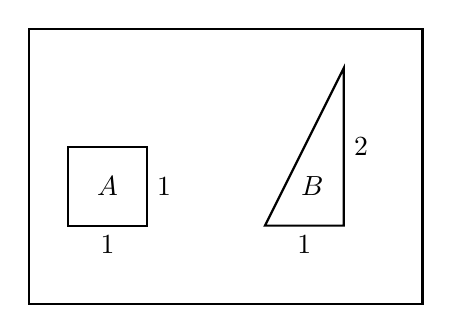
\begin{tikzpicture}[thick]
    \draw (0,0) rectangle (5,3.5);
    \draw (0.5,1) --node[below]{1}
    ++(1,0) -- node[right]{1}
    ++(0,1) -- ++(-1,0) -- cycle;
    \draw (3,1) -- node[below]{1}
    ++ (1,0)--node[right]{2}
    ++ (0,2) -- cycle;
    \draw (1,1.5)node{$A$} (3.6,1.5)node{$B$};
  \end{tikzpicture}
  \caption{落在度量相同的子区域内的等可能性.}
  \label{fig1.2.1}
  \end{minipage}%
  \begin{minipage}[b]{0.5\linewidth}
  \centering
  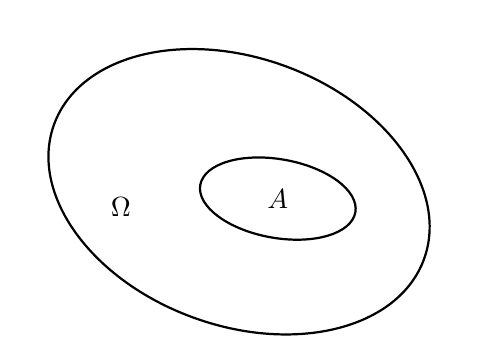
\begin{tikzpicture}[thick]
    \draw[rotate=-20] ellipse (2.5 and 1.7);
    \draw[rotate=-10,xshift=0.5cm] (0,0)node{$A$}
       ellipse (1 and 0.5);
    \node at (-1.5,-0.2) {$\Omega$};
  \end{tikzpicture}
  \caption{几何概率.}
  \label{fig1.2.2}
  \end{minipage}
\end{figure}

这个概率称为几何概率,
它满足概率的公理化定义.

求几何概率的关键是对样本空间 $\Omega$ 和所求事件 $A$ 用图形描述清楚 (一般用平面或空间图形).
然后计算出相关图形的度量 (一般为面积或体积).

\begin{example}[会商问题]
  甲乙两人约定在下午6时到7时之间在某处会面,
  并约定先到者应等候另一个人 \SI{20}{\minute},
  过时即可离去.
  求两人能会面的概率.
\end{example}

\begin{solution}
  以 $x$ 和 $y$ 分别表示甲、乙两人到达约会地点的时间 (以 \si{\minute} 为单位),
  在平面上建立 $xOy$ 直角坐标系 (见图~\ref{fig1.2.3}).

  \begin{figure}[!ht]
    \centering
    \begin{tikzpicture}[thick,>=Stealth]
    \draw[->] (-0.5,0) -- (0,0) node[below left]{$O$} -- (1,0) node[below]{20}
    -- (3,0)node[below]{60} -- (3.5,0)node[below]{$x$};
    \draw [->] (0,-0.5) -- (0,1) node[left]{20}
    -- (0,3) node[left]{60}
    -- (0,3.5) node[right] {$y$};
    \filldraw[pattern=vertical lines]
    (0,0) -- (1,0) -- (3,2) -- (3,3) --
    (2,3) -- (0,1) -- cycle;
    \draw (3,0) -- (3,2) (0,3) -- (2,3);
  \end{tikzpicture}
    \caption{会面问题中的 $\Omega$ 与 $A$.}
    \label{fig1.2.3}
  \end{figure}

  因为甲、乙都是在 0 至 \SI{60}{\minute} 内等可能地到达,
  所以由等可能性知这是一个几何概率问题.
  $(x, y)$ 的所有可能取值是边长为 60 的正方形,
  其面积为 $S_\Omega = 60^2$.
  而事件 $A =$“两人能够会面”相当于:
  \[
    | x - y | \le 20,
  \]
  即图中的阴影部分,
  其面积为 $S_A = 60^2 - 40^2$,
  由 \eqref{eq1.2.13} 式知
  \[
    P (A) = \frac{S_A}{S_\Omega} = \frac{60^2 - 40^2}{60^2} = 0.5556.
  \]
  结果表明:
  按此规则约会,
  两人能会面的概率不超过 0.6.
  若把约定时间改为在下午6时到6时30分,
  其他不变,
  则两人能会面的概率提高到 \num{0.8889}.
\end{solution}

\begin{example}[蒲丰投针问题]
  平面上画有间隔为 $d (d > 0)$ 的等距平行线,
  向平面任意投掷一枚长为 $l (l<d)$ 的针,
  求针与任一平行线相交的概率.
\end{example}

\begin{solution}
  以 $x$ 表示针的中点与最近一条平行线的距离,
  又以 $\varphi$ 表示针与此直线间的交角,
  见图~\ref{fig1.2.4}.
  易知样本空间 $\Omega$ 满足
  \[
    0 \le x \le d/2, \quad 0 \le \varphi \le \pi,
  \]
  由这两式可以确定 $x - \varphi$ 平面上的一个矩形 $\Omega$,
  这就是样本空间,
  其面积为 $S_\Omega = d\pi/2$.
  这时为了针与平行线相交 (记为事件 $A$),
  其充要条件是
  \[
    x \le \frac{l}{2} \sin \varphi.
  \]
  由这个不等式表示的区域是图~\ref{fig1.2.5} 中的阴影部分.

  由于针是向平面任意投掷的,
  所以由等可能性知这是一个几何概率问题.
  由此得
  \[
    P (A) = \frac{S_A}{S_\Omega}
    = \frac{\int_0^\pi \frac{l}{2} \sin \varphi \, \mathrm{d} \varphi}{\frac{d}{2} \pi}
    = \frac{2l}{d\pi}.
  \]

  如果 $l$, $d$ 为已知,
  则以 $\pi$ 的值代入上式即可计算得 $P(A)$ 之值.
  反之,
  如果已知 $P(A)$ 的值,
  则也可以利用上式去求 $\pi$,
  而关于 $P(A)$ 的值,
  可用从试验中获得的频率去近似它:
  即投针 $N$ 次,
  其中针与平行线相交 $n$ 次,
  则频率 $n/N$ 可作为 $P(A)$ 的估计值,
  于是由
  \[
    \frac{n}{N} \approx P (A) = \frac{2l}{d\pi},
  \]
  可得
  \[
    \pi \approx \frac{2lN}{dn}.
  \]

  历史上有一些学者曾亲自做过这个试验,
  下表记录了他们的试验结果.

  \begin{tabularx}{0.9\linewidth}{*{6}{Z}}
    \toprule
    试验者 & 年份 & $l/d$ & 投掷次数 & 相交次数 & $\pi$ 的近似值\\
    \midrule
    Wolf & 1850 & 0.8 & 5000 & 2532 & 3.1596\\
    Fox & 1884 & 0.75 & 1030 & 489 & 3.1595\\
    Lazzerini & 1901 & 0.83 & 3408 & 1808 & 3.1415\\
    Reina & 1925 & 0.54 & 2520 & 859 & 3.1795\\
    \bottomrule
  \end{tabularx}

  这是一个颇为奇妙的方法:
  只要设计一个随机试验,
  使一个事件的概率与某个未知数有关,
  然后通过重复试验,
  以频率估计概率,
  即可求得未知数的近似解.
  一般来说,
  试验次数越多,
  则求得的近似解就越精确。
  随着电子计算机的出现,
  入们便可利用计算机来大量重复地模拟所设计的随机试验。
  这种方法得到了迅速的发展和广泛的应用。
  入们称这种方法为\textbf{随机模拟法},
  也称为\textbf{蒙特卡罗 (Montecarlo) 法}.
\end{solution}

\begin{figure}
  \centering
  \begin{minipage}[b]{0.5\linewidth}
  \centering
  \begin{tikzpicture}[thick,>=Stealth,scale=1.2]
    \draw (-0.3,1) -- (4,1) (-0.3,-1)--(4,-1)
    node[below]{\phantom{$O$}};
    \draw[<->] (0,1) -- (0,-1)node[midway,fill=white]{$d$};
    \draw (2,1) -- +(45:0.3) --+ (-135:1.7);
    \draw (1.8,1) arc (180:225:0.2);
    \draw (1.51,1) --node[left]{$x$} ++(0,-0.49);
    \node at (1.7,0.85){$\varphi$};
  \end{tikzpicture}
   \caption{蒲丰投针问题}.
    \label{fig1.2.4}
  \end{minipage}%
  \begin{minipage}[b]{0.5\linewidth}
  \centering
  \begin{tikzpicture}[thick,>=Stealth]
    \draw[->](-0.3,0) -- (0,0)node[below]{$O$}
    -- (pi,0)node[below]{$\pi$} -- (4.2,0) node[below]{$\varphi$};
    \draw[->](0,0) -- (0,2.2)node[left]{$d/2$}
     -- (0,3) node[right]{$x$};
    \draw (0,2.2)--(pi,2.2)node[above right]{$\Omega$} -- (pi,0);
    \filldraw[pattern=north east lines]
    (0,0)-- plot[domain=0:pi,samples=100](\x,{1.3*sin(\x r)}) -- (pi,0)--cycle;
    \node at (1.57,1.6){$\frac l2\sin\varphi$};
  \end{tikzpicture}
  \caption{蒲丰投针问题中的 $\Omega$ 和 $A$}.
    \label{fig1.2.5}
  \end{minipage}
\end{figure}

\begin{example}
  在长度为 $a$ 的线段内任取两点将其分为三段,
  求它们可以构成一个三角形的概率.
\end{example}

\begin{solution}
  由于是将线段任意分成三段,
  所以由等可能性知这是一个几何概率问题.
  分别用 $x$, $y$ 和 $a - x - y$ 表示线段被分成的三段长度,
  见图~\ref{fig1.2.6}.
  则显然应该有
  \[
    0 < x < a; \quad 0 < y < a; \quad 0 < a - (x + y) < a.
  \]
  第三个式子等价于:
  $0 < x + y < a$.
  所以样本空间为 (见图~\ref{fig1.2.7})
  \[
    \Omega = \{(x, y): 0 < x < a, 0 < y < a, 0 < x + y < a\}.
  \]
  $\Omega$ 的面积为
  \[
    S _\Omega = \frac{a^2}{2}.
  \]

  又根据构成三角形的条件:
  三角形中任意两边之和大于第三边,
  得事件 $A$ 所含样本点 $(x,y)$ 必须满足:
  \begin{align*}
    & 0 < a - (x + y) < x + y,\\
    & 0 < x < y + (a - x - y),\\
    & 0 < y < x + (a - x - y).
  \end{align*}
  整理得
  \[
    \frac{a}{2} < x + y < a;\quad 0 < x < \frac{a}{2}; \quad 0 < y < \frac{a}{2}.
  \]
  所以事件 $A$ 可用图~\ref{fig1.2.8} 中的阴影部分表示.
  事件 $A$ 的面积为
  \[ S _A = \frac{a^2}{8}. \]
  由此得
  \[P (A) = \frac{1}{4}. \]
\end{solution}

\begin{figure}
  \begin{minipage}[b]{0.45\linewidth}
    \centering
    \begin{tikzpicture}[thick,>=Stealth,xscale=1.2]
    \draw (0,0) -- (4,0);
    \draw [densely dashed,yshift=-0.5cm](0,0) -- (4,0) node[midway,fill=white]{$a$};
    \foreach \x in {0,1,2.4,4}
      \draw(\x,-0.1) -- (\x,0.1);
    \draw[yshift=-0.5cm](0,-0.1)--(0,0.1)
    (4,-0.1)--(4,0.1);
    \draw (0.5,0.2)node{$x$} (1.7,0.2)node{$y$}
      (3.2,0.2)node{$a-x-y$};
  \end{tikzpicture}
    \caption{长度为 $a$ 的线段分成三段.}
    \label{fig1.2.6}
  \end{minipage}
  \begin{minipage}[b]{0.45\linewidth}
    \centering
    \begin{tikzpicture}[thick,>=Stealth,scale=2.6]
    \draw[->] (-0.2,0) --(1,0)node[below]{$a$}-- (1.5,0)node[below]{$x$};
    \draw[->] (0,-0.2) --(0,0)node[below left]{$O$}
    --(0,1)node[left]{$a$} -- (0,1.2)node[left]{$y$};
    \filldraw[pattern=horizontal lines] (0,0)--(1,0)
    --(0,1)--cycle;
  \end{tikzpicture}
    \caption{线段分成三段的样本空间 $\Omega$.}
    \label{fig1.2.7}
  \end{minipage}
\end{figure}

\begin{figure}
  \centering
  \begin{tikzpicture}[thick,>=Stealth,scale=2.6]
    \draw[->] (-0.2,0) --(1,0)node[below]{$a$}-- (1.5,0)node[below]{$x$};
    \draw[->] (0,-0.2) --(0,0)node[below left]{$O$}
    --(0,1)node[left]{$a$}--(0,1.2)node[left]{$y$};
    \draw (0,1) -- (1,0);
    \filldraw[pattern=horizontal lines]
    (0.5,0)node[below]{$1/2$} -- (0.5,0.5)
    --(0,0.5)node[left]{$1/2$} -- cycle;
  \end{tikzpicture}
  \caption{构成三角形的条件}
  \label{fig1.2.8}
\end{figure}

\subsection{确定概率的主观方法}

在现实世界里有一些随机现象是不能重复的或不能大量重复的,
这时有关事件的概率如何确定呢?

统计界的贝叶斯学派认为:
\textbf{一个事件的概率是人们根据经验对该事件发生的可能性所给出的个人信念}.
这样给出的概率称为\text{主观概率}.

这种利用经验确定随机享件发生可能性大小的例子是很多的,
人们也常依据某些主观概率来行事.

\begin{example}
  用主观方法确定概率的例子.
  \begin{enumerate}
    \item 在气象预报中,
    往往会说:“明天下雨的概率为 \SI{90}{\percent}”,
    这是气象专家根据气象专业知识和最近的气象情况给出的主观概率.
    听到这一信息的人,
    大多出门会带伞.

    \item 一个企业家根据他多年的经验和当时的一些市场信息,
    认为“某项新产品在未来市场上畅销”的可能性为 \SI{80}{\percent}.

    \item 一个外科医生根据自已多年的临床经验和一位患者的病情,
    认为“此手术成功”的可能性为 \SI{90}{\percent}.

    \item 一个教师根据自己多年的教学经验和甲、乙两学生的学习情况,
    认为“甲学生能考取大学”的可能性为 \SI{95}{\percent},
    “乙学生能考取大学”的可能性为 \SI{40}{\percent}.
  \end{enumerate}
\end{example}

从以上例子可以看出:
\begin{enumerate}
  \item 主观概率和主观臆造有着本质上的不同,
  前者要求当事人对所考察的事件有透彻的了解和丰富的经验,
  甚至是这一行的专家,
  并能对历史信息和当时信息进行仔细分析,
  如此确定的主观概率是可信的.
  从某种意义上说,
  不利用这些丰富的经验也是一种浪费.
  \item 用主观方法得出的随机事件发生的可能性大小,
  本质上是对随机事件概率的一种推断和估计.
  虽然结论的精确性有待实践的检验和修正,
  但结论的可信性在统计意义上是有其价值的.
  \item 在遇到的随机现象无法大量重复时,
  用主观方法去做决策和判断是适合的.
  从这点看,
  主观方法至少是频率方法的一种补充.
\end{enumerate}

另外要说明的是,
主观概率的确定除根据自己的经验外,
决策者还可以利用别人的经验。
例如,
对一项有风险的投资,
决策者向某位专家咨询的结果为“成功的可能性为 \SI{60}{\percent}”,
而决策者很熟悉这位专家,
认为专家的估计往往是偏保守的、过分蘧慎的.
为此决策者将结论修改为“成功的可能性为 \SI{70}{\percent}”.

主观给定的概率要符合公理化的定义.

\begin{xiti}
  \item 对于组合数 $\binom{n}{r}$, 证明
  \begin{enumerate}
    \item $\binom{n}{r} = \binom{n}{n - r}$;
    \item $\binom{n}{r} = \binom{n - 1}{r - 1} + \binom{n - 1}{r}$;
    \item $\binom{n}{0} + \binom{n}{1} + \dotsb + \binom{n}{n} = 2^n$;
    \item $\binom{n}{1} + 2\binom{n}{2} + \dotsb + n\binom{n}{n} = n 2^{n-1}$;
    \item $\binom{a}{0} \binom{b}{n} + \binom{a}{1} \binom{b}{n - 1} + \dotsb + \binom{a}{n} \binom{b}{0} = \binom{a + b}{n}$, $n = \min(a,b)$;
    \item $\binom{n}{0} ^2 + \binom{n}{1} ^2 + \dotsb + \binom{n}{n} ^2 = \binom{2n}{n}$.
  \end{enumerate}

  \item 抛两枚硬币,
  求至少出现一个正面的概率.

  \item 任取两个正整数,
  求它们的和为偶数的概率.

  \item 掷两颗骰子,
  求下列事件的概率:
  \begin{enumerate}
    \item 点数之和为7;
    \item 点数之和不超过5;
    \item 两个点数中一个恰是另一个的两倍.
  \end{enumerate}

  \item 考虑一元二次方程 $x^2 + Bx + C = 0$,
  其中 $B$, $C$ 分别是将一枚骰子接连掷两次先后出现的点数,
  求该方程有实根的概率 $p$ 和有重根的概率 $q$.

  \item 从一副52张的扑克牌中任取4张,
  求下列事件的概率:
  \begin{enumerate}
    \item 全是黑桃;
    \item 同花;
    \item 没有两张同一花色;
    \item 同色.
  \end{enumerate}

  \item 设5个产品中有3个合格品、2个不合格品.
  从中不返回地任取2个,
  求取出的2个中全是合格品、仅有一个合格品和没有合格品的概率各为多少?

  \item 口袋中有5个白球、3个黑球,
  从中任取两个,
  求取到的两个球颜色相同的概率.

  \item 甲口袋有5个白球、3个黑球,
  乙口袋有4个白球、6个黑球.
  从两个口袋中各任取一球,
  求取到射两个球颜色相同的概率.

  \item 从 $n$ 个数 $1, 2, \cdots, n$ 中任取2个,
  问其中一个小于 $k (1 < k < n)$,
  另一个大于 $k$ 的概率是多少?

  \item 口袋中有 10 只球,
  分别标有号码 1 到 10,
  从中不返回地任取 3 只,
  记下取出球的号码,
  试求:
  \begin{enumerate}
    \item 最小号码为5的概率;
    \item 最大号码为5的概率.
  \end{enumerate}

  \item 掷三颗骰子,
  求以下事件的概率:
  \begin{enumerate}
    \item 所得的最大点数小于等于5;
    \item 所得的最大点数等于5.
  \end{enumerate}

  \item 把10本书任意地放在书架上,
  求其中指定的三本书放在一起的概率.

  \item $n$ 个人隨机地圄一圆桌而坐,
  求甲、乙两人相邻而坐的概率.

  \item 5个人在第一层进入十一层楼的电梯.
  假如每个人以相同的概率走出任一层 (从第二层开),
  求此5个人在不同楼层走出的概率.

  \item 一个人把六根草紧在手中,
  仅露出它们的头和尾,
  然后随机地把六个头两两相接,
  六个尾也两两相接.
  求放开手后六根草恰巧连成一个环的概率.

  \item 把 $n$ 个“0”与 $n$ 个“1”随机地排列,
  求没有两个“1”连在一起的概率.

  \item 口袋中有 $n$ 个白球,
  $n$ 个黑球,
  从中一个一个不返回地摸球,
  直至摸完为止.
  求黑白球恰好相间取出的概率.

  \item $n$ 个男孩,
  $m$ 个女孩 ($m \le n + 1$) 随机地排成一排,
  试求任意两个女孩都不相邻的概率.

  \item 将3个球随机地放入4个杯子中去,
  求杯子中球的最大个数分别为1, 2, 3的概率各为多少?

  \item 将12只球随意地放人3个盒子中,
  试求第一个盒子中有3只球的概率.

  \item 将 $n$ 个完全相同的球 (这时也称球是不可辨的) 随机地放入 $N$ 个盒子中,
  试求:
  \begin{enumerate}
    \item 某个指定的盒子中恰好有 $k$ 个球的概率;
    \item 恰好有 $m$ 个空盒的概率;
    \item 某个指定的 $m$ 个盒子中恰好有 $j$ 个球的概率.
  \end{enumerate}

  \item 在区间 $(0,1)$ 中随机地取两个数,
  求事件“两数之和小于6/5”的概率.

  \item 甲乙两艘轮船驶向一个不能同时停泊两艘轮船的码头,
  它们在一昼夜内到达的时间是等可能的.
  如果甲船的停泊时间是一小时,
  乙船的停泊时间是两小时,
  求它们中任何一般都不需要等候码头空出的概率是多少?

  \item 在平面上画有间隔为 $d$ 的等距平行线,
  向平面任意投掷一个边长为 $a$, $b$, $c$ (均小于 $d$) 的三角形,
  求三角形与平行线相交的概率.

  \item 在半径为 $R$ 的圆内画平行弦,
  如果这些弦与垂直于弦的直径的交点在该直径上的位量是等可能的,
  即交点在直径上一个区间内的可能性与这区间的长度成比例,
  求任意弦的长度大于 $R$ 的概率.

  \item 设一个质点落在 $xOy$ 平面上由 $x$ 轴 $y$ 轴及直线 $x + y = 1$ 所围成的三角形内,
  而落在这三角形内各点处的可能性相等,
  即落在这三角形内任何区域上的概率与这区域的面积成正比,
  试求此质点落在直线 $x = 1/3$ 的左边的概率是多少?

  \item 设 $a > 0$,
  有任意两数 $x$, $y$,
  且 $0 < x < a$, $0 < y < a$,
  试求 $xy < a^2 / 4$ 的概率.

  \item 用主观方法确定:
  大学生中戴眼镜的概率是多少?

  \item 用主观方法确定:
  学生中考试作弊的概率是多少?
\end{xiti}

\section{概率的性质}
利用概率的公理化定义 (非负性、正则性和可列可加性),
可以导出概率的一系列性质.
以下我们逐个给出概率的一些常用性质.

首先,
在概率的正则性中说明了必然事件 $\Omega$ 的概率为1.
那么可想而知,
不可能事件 $\emptyset$ 的概率应该为0,
下面性质正说明了这一点.

\begin{property}
  \[
    P (\emptyset) = 0.
  \]
\end{property}

\begin{proof}
  由于可列个不可能事件之并仍是不可能事件,
  所以
  \[
    \Omega = \Omega \cup \emptyset \cup \emptyset \dotsb \cup \emptyset \cup \dotsb.
  \]
  因为不可能事件与任何事件是互不相容的,
  故由可列可邡性公理得
  \[
    P (\Omega) = P (\Omega) + P (\emptyset) + \dotsb + P (\emptyset) + \dotsb.
  \]
  从而由 $P (\Omega) = 1$ 得
  \[
    P (\Omega) + P (\emptyset) + \dotsb = 0.
  \]
  再由非负性公理,
  必有
  \[
    P (\emptyset) = 0.
  \]
  结论得证.
\end{proof}

\subsection{概率的可加性}

概率的可列可加性说明了对可列个互不相容的事件 $A_1$, $A_2$, $\dotsc$,
其可列并的概率可以分别求之再相加,
那么对有限个互不相容的事件 $A_1$, $A_2$, $\dotsc$, $A_n$,
其有限并的概率是否也可以分别求之再相加呢?
下面性质回答了这个问题.

\begin{property}[有限可加性]\label{prop1.3.2}
  若有限个事件 $A_1$, $A_2$, $\dotsc$, $A_n$ 互不相容,
  则有
  \begin{equation}
    P \biggl( \bigcup _{i=1} ^n A_i \biggr) = \sum_{i=1}^n P (A_i).
    \label{eq1.3.1}
  \end{equation}
\end{property}

\begin{proof}
  对 $A_1$, $A_2$, $\dotsc$, $A_n$, $\emptyset$, $\emptyset$, $\dotsc$,
  应用可列可加性,
  得
  \begin{align*}
    P \biggl( A_1\cup A_2 \cup \cdots \cup A_n \biggr)
    &= \biggl(  A_1\cup A_2 \cup \cdots \cup A_n \cup \emptyset \cup \emptyset \cup \cdots\biggr)\\
    &= P(A_1) + \cdots + P(A_n) + P (\emptyset) + P(\emptyset) + \cdots\\
    &= P(A_1) + \cdots + P(A_n).
  \end{align*}
  结论得证.
\end{proof}

由有限可加性,
我们就可以得到以下求对立事件概率的公式.

\begin{property}\label{prop1.3.3}
  对任一事件 $A$,
  有
  \begin{equation}
    P (\overline{A}) = 1 - P (A).
    \label{eq1.3.2}
  \end{equation}
\end{property}

\begin{proof}
  因为 $A$ 与 $\overline{A}$ 互不相容,
  且 $\Omega = A \cup \overline{A}$.
  所以由概率的正则性和有限可加性得 $1 = P(A) + P(\overline{A})$.
  由此得 $P(A) = 1 - P(\overline{A})$.
\end{proof}

有些事件直接考虑较为复杂,
而考虑其对立事件则相对比较简单.
对此类问题就可以利用性质~\ref{prop1.3.3},
见下面例子.

\begin{example}
  36只灯泡中4只是 \SI{60}{\watt},
  其余都是 \SI{40}{\watt} 的.
  现从中任取3只,
  求至少取到一只 \SI{60}{\watt} 灯泡的概率.
\end{example}

\begin{solution}
  记事件 $A$ 为“取出的3只中至少有一只 \SI{60}{\watt}”,
  则 $A$ 包括三种情况:
  取到一只 \SI{60}{\watt} 两只 \SI{40}{\watt},
  或取到两只 \SI{60}{\watt} 一只 \SI{40}{\watt},
  或取到三只 \SI{60}{\watt}.
  而 $A$ 的对立事件 $\overline{A}$ 只包括一种情况,
  即“取出的3只全部是 \SI{40}{\watt}”,
  由例~\ref{exmp1.2.3} 抽样模型可知
  \[
    P(\overline{A}) = \frac{\binom{32}{3}}{\binom{36}{3}}
    = \frac{248}{357} = 0.695.
  \]
  所以
  \[
    P(A) = 1 - P(\overline{A}) = \frac{109}{357} = 0.305.
  \]
\end{solution}

\begin{example}
  抛一枚硬币5次,
  求既出现正面又出现反面的概率.
\end{example}

\begin{solution}
  记事件 $A$ 为“抛5次硬币中既出现正面又出现反面”,
  则 $A$ 的情况较复杂,
  因为出现正面的次数可以是1次至4次,
  而 $A$ 的对立事件则相对简单:
  5次全部是正面 (记为 $B$),
  或5次全部是反面 (记为 $C$),
  即 $A = B \cup C$,
  其中 $B$ 与 $C$ 互不相容.
  所以由对立事件公式和概率的有限可加性得
  \begin{align*}
    P (A) &= 1 - P (\overline{A}) = 1 - P (B \cup C) = 1 - P (B) - P (C)\\
    &= 1 - \frac{1}{2^5} - \frac{1}{2^5} = \frac{15}{16}.
  \end{align*}
\end{solution}

\subsection{概率的单调性}

可以想象:
当 $B$ 被 $A$ 包含时 (即 $B$ 发生必然导致 $A$ 发生),
说明事件 $A$ 比事件 $B$ 更容易发生,
那么 $B$ 的概率不应该比 $A$ 的概率大,
这可由以下性质~\label{property1.3.4} 的推论说明之.

性质~\label{property1.3.4} 给出了两个有包含关系事件差的概率公式,
而性质~\label{property1.3.5} 给出了任意两个事件差的概率公式.

\begin{property}\label{property1.3.4}
  若 $A \supset B$,
  则
  \begin{equation}
    P (A - B) = P (A) - P (B).
    \label{eq1.3.3}
  \end{equation}
\end{property}

\begin{proof}
  因为 $A \supset B$,
  所以
  \[
    P (A - B) = B \cup (A - B),
  \]
  且 $B$ 与 $A - B$ 互不相容,
  由有限可加性得
  \[
    P (A) = P (B) + P (A - B),
  \]
  即得
  \[
    P (A - B) = P (A) - P (B).
  \]
  结论得证.
\end{proof}

\begin{corollary}{}
  若 $A \supset B$,
  则 $P (A) \ge P (B)$.
\end{corollary}

很容易举例说明:
以上推论的逆命题不成立,
即由 $P (A) \ge P (B)$ 无法推出 $A \supset B$.

\begin{property}\label{property1.3.5}
  对任意两个事件 $A$, $B$, 有
  \begin{equation}
    P (A - B) = P (A) - P (AB).
    \label{eq1.3.4}
  \end{equation}
\end{property}

\begin{proof}
  因为 $A - B = A - AB$,
  且 $AB \subset A$,
  所以由性质~\label{property1.3.4} 得
  \[
     p (A - B) = P (A - AB) = P (A) - P (AB).
  \]
  结论得证.
\end{proof}

利用性质~\label{property1.3.4},
我们可以求一些较为复杂的事件的概率.

\begin{example}
  口袋中有编号为 1, 2, \dots, $n$ 的 $n$ 个球,
  从中有放回地任取 $m$ 次,
  求取出的 $m$ 个球的最大号码为 $k$ 的概率.
\end{example}

\begin{solution}
  记事件 $A_k$ 为“取出的 $m$ 个球的最大号码为 $k$”.
  如果直接考虑事件 $A_k$,
  则比较复杂,
  因为“最大号码为 $k$”可以包括取到1次 $k$、取到2次 $k$、\dots、取到 $m$ 次$k$.

  为此我们记事件 $B_i$ 为“取出的 $m$ 个球的最大号码小于等于 $i$”, $i=1$, $2$, $\dotsc$, $n$.
  则 $B$ 发生只需每次从 $1$, $2$, $\dotsc$, $i$ 号球中取球即可.
  所以由古典概率知
  \[
    P(B_i) = \frac{i^m}{n^m}, \quad i = 1, 2, \dotsc, n.
  \]
  又因为 $A_k = B_k - B_{k-1}$,
  且 $B_{k-1} \subset B_k$,
  由性质~\label{property1.3.4} 得
  \begin{align*}
    P(A_k) &= P(B_k - B_{k-1}) = P(B_k) - P(B_{k-1})\\
    &= \frac{k^m - (k - 1)^m}{n^m}, \quad k = 1,2, \dotsc, n.
  \end{align*}

  譬如,
  $n = 6$, $m = 3$,
  可算得
  \[
    P(A_4) = \frac{4^3 - 3^3}{6^3} = \frac{37}{216} = 0.1713.
  \]
  其他的 $P(A_k)$ 也都可算出,
  现列表如下:

  \begin{tabularx}{\linewidth}{*{8}{Z}}
    \toprule
    $k$ & 1 & 2 & 3 & 4 & 5 & 6 & 和\\
    \midrule
    $P(A_k)$ & 0.0046 & 0.0324 & 0.0880 & 0.1713 & 0.2824 & 0.4213 & 1.000\\
    \bottomrule
  \end{tabularx}

  这相当于掷三颗骰子,
  最大点数为6的概率是0.4213,
  而由
  \[
    P(k \le 3) = 0.0046 + 0.0324 + 0.0880 = 0.1250.
  \]
  说明:
  掷三颗骰子,
  最大点数不超过3的概率仅为0.1250.
\end{solution}

\subsection{概率的加法公式}

当事件之间互不相容时,
有限可加性或可列可加性给出了求事件并的概率的公式。
那么对一般的事件 (不一定互不相容),
又如何求事件并的概率?
以下性质~\label{property1.3.6} 给出求任意两个事件并的概率加法公式,
\eqref{eq1.3.6} 给出求任意 $n$ 个事件并的概率加法公式.
这些性质在计算概率时是非常有用的.

\begin{property}[加法公式]\label{property1.3.6}
  对任意两个事件 $A$, $B$, 有
  \begin{equation}
    P(A \cup B) = P(A) + P(B) - P(AB).
    \label{eq1.3.5}
  \end{equation}
  对任意 $n$ 个事件 $A_1$, $A_2$, $\dotsc$, $A_n$, 有
  \begin{multline}
    P \biggl( \bigcup_{i=1}^n A_i \biggr) = \sum_{i=1}^n P (A_i)
    - \sum_{1 \le i < j < \le n} P(A_i A_j)
    + \sum_{1 \le i < j < k \le n} P(A_i A_j A_k)\\
    + \dotsb + (-1)^{n-1} P(A_1 A_2 \dotsb A_n).
    \label{eq1.3.6}
  \end{multline}
\end{property}

\begin{proof}
  先证 \eqref{eq1.3.5}. 因为
  \[
    A \cup B = A \cup (B - A),
  \]
  且 $A$ 与 $B - A$ 互不相容,
  所以由有限可加性和性质~\label{property1.3.5}得
  \[
    P (A \cup B) = P (A) + P (B - A) = P (A) + P (B) - P(AB).
  \]

  下面用归纳法证明 \eqref{eq1.3.6}.
  当 $n=2$ 时,
  \eqref{eq1.3.6} 即为 \eqref{eq1.3.5}.
  设 \eqref{eq1.3.6} 对 $n - 1$ 成立,
  则对 $n$,
  先对两个事件 $(A_1 \cup A_2 \cup \dotsb \cup A_{n-1})$ 与 $A_n$ 用 \eqref{eq1.3.5},
  \begin{align*}
    P (A_1 \cup A_2 \cup \dotsb \cup A_n)
    &= P (A_1 \cup A_2 \cup \dotsb \cup A_{n-1}) + P (A_n)
    - P ( (A_1 \cup A_2 \cup \dotsb \cup A_{n-1}) \cap A_n )\\
    &= P (A_1 \cup A_2 \cup \dotsb \cup A_{n-1}) + P (A_n)
    - P ( (A_1 A_n) \cup (A_2 A_n) \cup \dotsb \cup (A_{n-1} A_n) ).
  \end{align*}
  然后由归纳假设,
  对
  \[
    P (A_1 \cup A_2 \cup \dotsb \cup A_{n-1})
    \quad \text{及} \quad
    P ( (A_1 A_n) \cup (A_2 A_n) \cup \dotsb \cup (A_{n-1} A_n) )
  \]
  进行展开,
  经过整理合并即可知:
  \eqref{eq1.3.6} 对 $n$ 也成立,
  结论得证.
\end{proof}

\begin{corollary}{半可加性}
  对任意两个事件 $A$, $B$,
  有
  \begin{equation}
    P (A \cup B) \le P (A) + P (B).
    \label{eq1.3.7}
  \end{equation}
  对任意 $n$ 个事件 $A_1$, $A_2$, $\dotsc$, $A_n$,
  有
  \begin{equation}
    P \biggl( \bigcup _{i=1} ^n A_i \biggr) \le \sum _{i=1} ^n P (A_i).
    \label{eq1.3.8}
  \end{equation}
\end{corollary}

\begin{example}
  已知事件 $A$, $B$, $A \cup B$ 的概率分别为 0.4, 0.3, 0.6,
  求 $P (A \overline{B})$.
\end{example}

\begin{solution}
  由加法公式及题没条件知:
  \[
    0.6 = 0.4 + 0.3 - P (AB),
  \]
  由此解得 $P (AB) = 0.1$,
  所以再由 \eqref{eq1.3.4} 得
  \[
    P (A \overline{B}) = P (A - B) = P (A) - P (AB) = 0.4 - 0.1 = 0.3.
  \]
\end{solution}

\begin{example}
  已知 $P (A) = P (B) = P (C) = 1/4$,
  $P (AB) = 0$,
  $P (AC) = P (BC) = 1/16$.
  则 $A$, $B$ ,$C$ 中至少发生一个的概率是多少?
  $A$, $B$, $C$ 都不发生的概率是多少?
\end{example}

\begin{solution}
  因为 $P (AB) = 0$,
  且 $ABC \subset AB$,
  所以由概率的单调性知 $P (ABC) = 0$.
  再由加法公式,
  得 $A$, $B$, $C$ 中至少发生一个的概率为
  \begin{align*}
    P (A \cup B \cup C)
    &= P (A) + P (B) + P (C) - P (AB) - P (AC) - P (BC) + P (ABC)\\
    &= \frac{3}{4} - \frac{2}{16} = \frac{5}{8}.
  \end{align*}

  又因为“$A$, $B$, $C$ 都不发生”的对立事件为“$A$, $B$, $C$ 中至少发生一个”,
  所以由对立事件公式得
  \[
    P (A, B, C \text{ 都不发生}) = 1 - \frac{5}{8} = \frac{3}{8}.
  \]
\end{solution}

一般而言,
求“至少有一个……”的概率时,
用对立事件公式去求较为方便.
但下面例~\ref{exam1.3.6} 的配对问题却不能用对立事件去求解,
而一定要将事件“至少有个……”表示成事件的并,
然后用一般事件的加法公式去求解.

\begin{example}[配对问题]\label{exam1.3.6}
  在一个有 $n$ 个人参加的晚会上,
  每个人带了一件礼物,
  且假定各人带的礼物都不相同.
  晚会期间各人从放在一起的 $n$ 件礼物中随机抽取一件,
  问至少有一个人自己抽到自己礼物的概率是多少?
\end{example}

\begin{solution}
  以 $A_i$ 记事件“第 $i$ 个人自己抽到自己的礼物”,
  $i=1,\dotsc,n$.
  所求概率为 $P(A_1 \cup A_2 \cup \dotsb \cup A_n)$.
  因为
  \begin{align*}
    & P(A_1) = P(A_2) = \dotsb = P(A_n) =\frac{1}{n},\\
    & P(A_1 A_2) = P(A_1 A_3) = \dotsb = P(A_{n-1} A_n) = \frac{1}{n (n-1)},\\
    & P(A_1 A_2 A_3) = P(A_1 A_2 A_4) = \dotsb = P(A_{n-2} A_{n-1} A_n) = \frac{1}{n (n-1) (n-2)},\\
    & \ldots\\
    & P(A_1 A_2 \dotsb A_n) = \frac{1}{n!}.
  \end{align*}
  所以由概率的加法公式 \eqref{eq1.3.6} 得
  \[
    P(A_1 \cup A_2 \cup \dotsb \cup A_n) = 1 - \frac{1}{2!} + \frac{1}{3!} - \frac{1}{4!} + \dotsb + (-1)^{n-1} \frac{1}{n!}.
  \]
  譬如,
  当 $n=5$ 时,
  此概率为 \num{0.6333};
  当 $n \ge 10$ 时,
  此概率近似为 $1 - e^{-1} = 0.6321$.
  这表明:
  即使参加晚会的人很多 (譬如 100 人以上),
  事件“至少有一个人自己抽到自己礼物”也不是必然事件.
\end{solution}

\subsection{概率的连续性}

为了讨论概率的连续性,
我们先对事件序列的极限给出如下的定义.

\begin{definition}{}{1.3.1}
  \begin{enumerate}
    \item 对 $\mathscr{F}$ 中任一单调不减的事件序列 $F_1 \subset F_2 \subset \dotsb \subset F_n \subset \dotsb$,
    称可列并 $\bigcup_{n=1}^{+\infty} F_n$ 为 $\{ F_n \}$ 的\textbf{极限事件},
    记为
    \begin{equation}
      \lim_{n \to +\infty} F_n = \bigcup_{n=1}^{+\infty} F_n.
      \label{eq1.3.9}
    \end{equation}

    \item 对 $\mathscr{F}$ 中任一单调不增的事件序列 $E_1 \supset E_2 \supset \dotsb \supset E_n \supset \dotsb$,
    称可列交 $\bigcap_{n=1}^{+\infty} E_n$ 为 $\{ E_n \}$ 的\textbf{极限事件},
    记为
    \begin{equation}
      \lim _{n \to +\infty} E _n = \bigcap _{n=1} ^{+\infty} E_n.
      \label{eq1.3.10}
    \end{equation}
  \end{enumerate}
\end{definition}

有了以上极限事件的定义,
我们就可如下给出一个概率函数的连续性定义.

\begin{definition}{}{1.3.2}
  对 $\mathscr{F}$ 上的一个概率 $P$,
  \begin{enumerate}
    \item 若它对 $\mathscr{F}$ 中任一单调不减的事件序列 $\{F_n\}$ 均成立
    \[
      \lim _{n \to +\infty} P (F_n) = P (\lim _{n \to +\infty} F_n),
    \]
    则称概率 $P$ 是\textbf{下连续}的.

    \item 若它对 $\mathscr{F}$ 中任一单调不增的事件序列 $\{E_n\}$ 均成立
    \[
      \lim _{n \to +\infty} P (E_n) = P (\lim _{n \to +\infty} E_n),
    \]
    则称概率 $P$ 是\textbf{上连续}的.
  \end{enumerate}
\end{definition}

有了以上的定义,
我们就可以证明概率的连续性了.

\begin{property}[概率的连续性]\label{prop1.3.7}
  若 $P$ 为事件域上的概率,
  则 $P$ 既是下连续的,
  又是上连续的.
\end{property}

\begin{proof}
  先证 $P$ 的下连续性.
  设 $\{F_n\}$ 是 $\mathscr{F}$ 中一个单调不减的事件序列,
  即
  \[
    \bigcup _{i=1} ^{+\infty} F_i = \lim _{n \to +\infty} F_n.
  \]
  若定义 $F_0 = \emptyset$,
  则
  \[
    \bigcup _{i=1} ^{+\infty} F_i = \bigcup _{i=1} ^{+\infty} (F_i - F_{i-1}).
  \]
  由于 $F_{i-1} \subset F_i$,
  显然诸 $(F_i, F_{i-1})$ 两两不相容,
  再由可列可加性得
  \[
    P \biggl( \bigcup _{i=1} ^{+\infty} F_i \biggr) = \sum _{i=1} ^{+\infty} P (F_i - F_{i-1}) = \lim_{n \to +\infty} \sum _{i=1} ^n P (F_i - F_{i-1}).
  \]
  又由有限可加性得
  \[
    \sum _{i=1} ^n P (F_i - F_{i-1}) = P \biggl( \bigcup _{i=1} ^n (F_i - F_{i-1}) \biggr) = P (F_n).
  \]
  所以
  \[
    P (\lim _{n \to +\infty} F_n) = \lim _{n \to +\infty} P (F_n).
  \]
  这就证得了 $P$ 的下连续性.

  再证 $P$ 的上连续性.
  设 $\{ E_n \}$ 是单调不增的事件序列,
  则 $\{ \overline{E}_n \}$ 为单调不减的事件序列,
  由概率的下连续性得
  \begin{align*}
    1 - \lim _{n \to +\infty} P (E_n)
    &= \lim _{n \to +\infty} [1 - P (E_n)] = \lim _{n \to +\infty} P (\overline{E} _n)\\
    &= P \biggl( \bigcup _{n=1} ^{+\infty} \overline{E}_n \biggr)
    = P \biggl( \overline{\bigcap _{n=1} ^{+\infty} E_n} \biggr)\\
    &= 1 - P \biggl( \bigcap _{n=1} ^{+\infty} E_n \biggr).
  \end{align*}
  注意最后第二个等式用了德莫根公式.
  至此得
  \[
    \lim _{n \to +\infty} P (E_n) = P \biggl( \bigcap _{n=1} ^{+\infty} E_n \biggr).
  \]
  这就证得了 $P$ 的上连续性.
\end{proof}

下面我们对可列可加性作进一步讨论.
从上面的讨论可知,
由可列可加性可推出有限可加性和下连续性,
但由有限可加性不能推出可列可加性.
这意味着要由有限可加性去推可列可加性,
还缺少条件.
下面性质说明:
所缺少的条件就是下连续性.

\begin{property}\label{prop1.3.8}
  若 $P$ 是 $\mathscr{F}$ 上满足 $P(\Omega) = 1$ 的非负集合函数,
  则它具有可列可加性的充要条件是 (1) 它是有限可加的; (2) 它是下连续的.
\end{property}

\begin{proof}
  必要性可从性质~\ref{prop1.3.2} 和性质~\ref{prop1.3.7} 获得.
  下证充分性.

  设 $A_i \in \mathscr{F}$, $i=1,2,\dotsc$ 是两两不相容的事件序列,
  由有限可加性可知:
  对任意有限的 $n$ 都有
  \[
    P \biggl( \bigcup _{i=1} ^n A_i \biggr) = \sum _{i=1} ^n P (A_i).
  \]
  这个等式的左边不超过1,
  因此正项级数 $\sum _{i=1} ^{+\infty} P (A_i)$ 收敛,
  即
  \begin{equation}
    \lim _{n \to +\infty} P \biggl( \bigcup _{i=1} ^n A_i \biggr)
    = \lim _{n \to +\infty} \sum _{i=1} ^n P (A_i)
    = \sum _{i=1} ^{+\infty} P (A_i).
    \label{eq1.3.11}
  \end{equation}
  记
  \[
    F_i = \bigcup _{i=1} ^n A_i,
  \]
  则 $\{Fn\}$ 为单调不减的事件序列,
  所以由下连续性得
  \begin{equation}
    \lim _{n \to +\infty} P \biggl( \bigcup _{i=1} ^n A_i \biggr)
    = \lim _{n \to +\infty} P (F_n)
    = P \biggl( \bigcup _{n=1} ^{+\infty} F_n \biggr)
    = P \biggl( \bigcup _{n=1} ^{+\infty} A_n \biggr).
    \label{eq1.3.12}
  \end{equation}
  综合 \eqref{eq1.3.11} 和 \eqref{eq1.3.12},
  即得可列可加性.
\end{proof}

从性质~\ref{prop1.3.8} 可以看出:
在概率的公理化定义中,
可以将可列可加性换成是有限可加性和下连续性.

\begin{xiti}
  \item 对下述五个事件发生可能性的文宇插述找出最合适的数值答案:\\
  \begin{tabularx}{0.7\linewidth}{p{0.5\linewidth}l}
    \toprule
    文字描述 & 数值答案\\
    \midrule
    (1) 事件 $A$ 发生与不发生的可能性一样 & (a) 0\\
    (2) 事件 $B$ 很可能发生, 但不一定发生 & (b) 0.1\\
    (3) 事件 $C$ 肯定不发生 & (c) 0.5\\
    (4) 事件 $D$ 能够发生, 但可能性不大 & (d) 0.9\\
    (5) 事件 $E$ 必定会发生 & (e) 1\\
    \bottomrule
  \end{tabularx}

  \item 设 $P (AB) = 0$,
  则下列说法哪些是正确的?
  \begin{enumerate}
    \item $A$ 和 $B$ 不相容;
    \item $A$ 和 $B$ 相容;
    \item $AB$ 是不可能事件;
    \item $AB$ 不一定是不可能事件;
    \item $P(A) = 0$, 或 $P(B) = 0$;
    \item $P(A-B) = P(A)$.
  \end{enumerate}

  \item 一批产品分一、二、三级,
  其中一级品是二级品的两倍,
  三级品是二级品的一半,
  从这批产品中随机地抽取一个,
  试求取到二级品的概率.

  \item 从0, 1, 2, \dots,9 等十个数字中任意选出三个不同的数字,
  试求下列事件的概率:
  \begin{enumerate}
    \item $A_1 = \{ \text{三个数字中不含 0 和 5} \}$;
    \item $A_2 = \{ \text{三个数字中不含 0 或 5} \}$;
    \item $A_3 = \{ \text{三个数字中含 0 但不含 5} \}$.
  \end{enumerate}

  \item 某城市中共发行3种报纸 A, B, C.
  在这城市的居民中有 \SI{45}{\percent} 订阅 A 报、\SI{35}{\percent} 订阅 B 报、\SI{30}{\percent} 订阅 C 报,
  \SI{10}{\percent} 同时订阅 A 报 B 报、\SI{8}{\percent} 同时订阅 A 报 C 报、\SI{5}{\percent} 同时订阅 B 报 C 报、\SI{3}{\percent} 同时订阅 A, B, C 报.
  求以下事件的百分率:
  \begin{enumerate}
    \item 只订阅 A 报的;
    \item 只订阅一种报纸的;
    \item 至少订阅一种报纸的;
    \item 不订阅任何一种报纸的.
  \end{enumerate}

  \item 某工厂一个班组共有男工7人、女工4人,
  现要选出3个代表,
  问选的3个代表中至少有1个女工的概率是多少?

  \item 赌徒认为掷一颗骰子4次至少出现一次6点与掷两颗骰子24次至少出现一次双6点的机会是相等的,
  你认为如何?

  \item 从数字1, 2, \dots, 9中可重复地任取 $n$ 次,
  求 $n$ 次所取数字的乘积能被10整除的概率.

  \item 口袋中有 $n-1$ 个黑球和 1 个白球,
  每次从口袋中随机地摸出一球,
  并换入一只黑球.
  问第 $k$ 次摸球时,
  摸到黑球的概率是多少?

  \item 甲掷硬币 $n+1$ 次,
  乙掷 $n$ 次.
  求甲掷出的正面数比乙掷出的正面数多的概率.

  \item 掷 $2n+1$ 次硬币,
  求出现的正面数多于反面数的概率.

  \item 有三个人,
  每个人都以同样的概率 $1/4$ 被分配到四个房间中的每一间中,
  试求:
  \begin{enumerate}
    \item 三个人都分配到同一个房间的概率;
    \item 三个人分配到不同房间的概率.
  \end{enumerate}

  \item 一间宿舍内住有6位同学,
  求他们之中至少有2个人的生日在同一个月份的概率.

  \item 某班 $n$ 个战士各有1支归个人保管使用的枪,
  这些枪的外形完全一样,
  在一次夜间紧急集合中,
  每人随机地取了1支枪,
  求至少有1人拿到自己的枪的概率.

  \item 设 $A$, $B$ 是两事件,
  且 $P(A) = 0.6$,
  $P(B) = 0.7$,
  问:
  \begin{enumerate}
    \item 在什么条件下 $P(AB)$ 取到最大值,
    最大值是多少?
    \item 在什么条件下 $P(AB)$ 取到最小值,
    最小值是多少?
  \end{enumerate}

  \item 已知事件 $A$, $B$ 满足 $P(AB) = P(\overline{A} \cap \overline{B})$,
  记 $P(A) = p$,
  试求 $P(B)$.

  \item 已知 $P(A) = 0.7$,
  $P(A-B) = 0.3$,
  试求 $P(\overline{AB})$.

  \item 设 $P(A) = P(B) = 1/2$,
  试证 $P(AB) = P(A \cap B)$.

  \item 对任意的事件 $A$, $B$, $C$,
  证明:
  \begin{enumerate}
    \item $P (AB) + P (AC) - P (BC) \le P (A)$,
    \item $P (AB) + P (AC) + P (BC) \ge P (A) + P (B) + P (C) - 1$.
  \end{enumerate}

  \item 设 $A$, $B$, $C$ 为三个事件,
  且 $P(A) = a$, $P(B) = 2a$, $P(C) = 3a$,
  $P(AB) = P(AC) = P(BC) = b$,
  证明:
  $a \le 1/4$, $b \le 1/4$.

  \item 设事件 $A$, $B$, $C$ 的概率都是1/2,
  且 $P(ABC) = P(\overline{A} \cap \overline{B} \cap \overline{C})$,
  证明:
  \[
    2P(ABC) = P(AB) + P(AC) + P(BC) / 1/2.
  \]

  \item 证明:
  \begin{enumerate}
    \item $P(AB) \ge P(A) + P(B) - 1$,
    \item $P(A_1 A_2 \dotsb A_n) \ge P(A_1) + P(A_2) + \dotsb + P(A_n) - (n-1)$.
  \end{enumerate}

  \item 证明:
  \[
    \lvert P(AB) - P(A)P(B) \rvert \le \frac{1}{4}.
  \]
\end{xiti}

\section{条件概率}

条件概率是概率论中的一个既重要又实用的概念。

\subsection{条件概率的定义}

所谓条件概率,
它是指在某事件 $B$ 发生的条件下,
求另一事件 $A$ 的概率,
记为 $P(A|B)$,
它与 $P(A)$ 是不同的两类概率.
下面用一个例子说明之.

\begin{example}
  考察有两个小孩的家庭,
  其样本空间为 $\Omega = \{bb,bg,gb,gg\}$,
  其中 $b$ 代表男孩,
  $g$ 代表女孩,
  $bg$ 表示大的是男孩、小的是女孩,
  其他样本点可类似说明.

  在 $\Omega$ 中4个样本点等可能情况下,
  我们来讨论如下一些事件的概率.
  \begin{enumerate}
    \item 事件 $A=$“家中至少有一个女孩”发生的概率为
    \[
      P(A) = \frac{3}{4}.
    \]

    \item 若已知事件 $B=$“家中至少有一个男孩”发生,
    再求事件 $A$ 发生的概率为
    \[
      P(A|B) = \frac{2}{3}.
    \]
    这是因为事件 $B$ 的发生,
    排除了 $gg$ 发生的可能性,
    这时样本空间 $\Omega$ 也随之改为 $\Omega_B = \{bb,bg,gb\}$,
    而在 $\Omega_B$ 中事件 $A$ 只含2个样本点,
    故 $P(A|B) = 2/3$.
    这就是条件概率,
    它与 (无条件) 概率 $P (A)$ 是不同的两个概念.

    \item 若对上述条件概率的分子分母各除以4,
    则可得
    \[
      P(A|B) = \frac{2/4}{3/4} = \frac{P(AB)}{P(B)},
    \]
    其中交事件 $AB=$“家有一男一女两个小孩”.
  \end{enumerate}
\end{example}

这个关系具有一般性,
即条件概率是两个无条件概率之商,
这就是条件概率的定义.

\begin{definition}{}{1.4.1}
  设 $A$ 与 $B$ 是样本空间 $\Omega$ 中的两事件,
  若 $P(B) > 0$,
  则称
  \begin{equation}
    P(A|B) = \frac{P(AB)}{P(B)}.
    \label{eq1.4.1}
  \end{equation}
  为“\textbf{在 $B$ 发生下 $A$ 的条件概率}”,
  简称\textbf{条件概率}.
\end{definition}

\begin{example}\label{exam1.4.2}
  设某样本空间 $\Omega$ 含有25个等可能的样本点,
  事件 $A$ 含有15个样本点,
  事件 $B$ 含有7个样本点,
  交事件 $AB$ 含有5个样本点,
  具体见图~\ref{fig1.4.1}.

  \begin{figure}
    \centering
    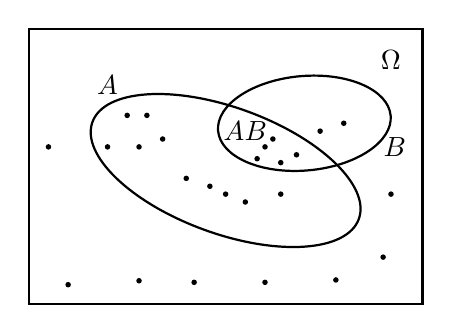
\begin{tikzpicture}[thick]
  \draw (0,0) rectangle (5,3.5);
  \draw[rotate around={-20:(2.5,1.7)}](2.5,1.7) circle (1.8 and 0.8);
  \draw[rotate around={5:(3.5,2.3)}] (3.5,2.3) ellipse (1.1 and 0.6);
  \node at (4.6,3.1) {$\Omega$};
  \node at (2.75,2.2) {$AB$};
  \node at (4.65,2) {$B$};
  \node at (1,2.78) {$A$};
  \foreach \x/\y in {
    3/2, 2.9/1.85, 3.1/2.1, 3.2/1.8, 3.4/1.9,
    3.7/2.2, 4/2.3,
    0.25/2, 0.5/0.25, 1.4/0.3, 2.1/0.28,
    3/0.28, 3.9/0.31, 4.5/0.6, 4.6/1.4,
    1/2, 1.25/2.4, 1.5/2.4, 1.7/2.1, 1.4/2,
    2/1.6, 2.3/1.5, 2.5/1.4, 2.75/1.3, 3.2/1.4
  }
  \fill(\x,\y) circle(1pt);
\end{tikzpicture}
    \caption{例~\ref{exam1.4.2} 的维恩图.}\label{fig1.4.1}
  \end{figure}

  这时有
  \begin{align*}
    & P(A) = \frac{15}{25},\\
    & P(B) = \frac{7}{25},\\
    & P(AB) = \frac{5}{25}.
  \end{align*}
  则在事件 $B$ 发生的条件下,
  事件 $A$ 的条件概率为
  \[
    P (A|B) = \frac{P(AB)}{p(B)} = \frac{5/25}{7/25} = \frac{5}{7}.
  \]

  此结果也可以如此考虑:
  事件 $B$ 发生,
  表明事件 $\overline{B}$ 不可能发生,
  因此 $\overline{B}$ 中的18个样本点可以不予考虑.
  此时在 $B$ 中7个样本点中属于 $A$ 的只有5个,
  所以 $P(A|B) = 5/7$.
  这意味着,
  在计算条件概率 $P(A|B)$ 时,
  样本空间 $\Omega$ 缩小为 $\Omega_B = B$.

  类似地
  \[
    P (B|A) = \frac{P(AB)}{P(A)} = \frac{5/25}{15/25} = \frac{1}{3}.
  \]
  它也可作如上解释.
\end{example}

我们要注意的是:
条件概率 $P(A|B)$ 是在给定 $B$ 下讨论事件 $A$ 的概率,
那么概率的性质对 $P(\cdot|B)$ 而言是否都成立呢?
譬如
\[
  P (\overline{A} | B) = 1 - P(A|B),
\]
\[
  P(A_1 \cup A_2 | B) = P(A_1 | B) + P(A_2 | B) - P(A_1 A_2 | B)
\]
这些概率性质都成立吗?
为此我们只要能验证条件概率满足三条公理即可回答这个问题.

\begin{property}
  条件概率是概率,
  即若设 $P(B) > 0$,
  则
  \begin{enumerate}
    \item $P(A|B) \ge 0$, $A \in \mathscr{F}$,
    \item $P(\Omega|B) = 1$,
    \item 若 $\mathscr{F}$ 中的 $A_1$, $A_2$,\dots,$A_n$,\dots 互不相容,
    则
    \[
      P \biggl( \bigcup _{n=1} ^{+\infty} A_n | B \biggr) = \sum_{n=1} ^{+\infty} P (A_n | B).
    \]
  \end{enumerate}
\end{property}

\begin{proof}
  用条件概率的定义很容易证明前两点.
  下面来证明第三点.
  因为 $A_1$, $A_2$, \dots, $A_n$, \dots 互不相容,
  所以 $A_1B$, $A_2B$, \dots, $A_nB$, \dots 也互不相容,
  故
  \begin{align*}
    P \biggl( \bigcup _{n=1} ^{+\infty} A_n | B \biggr)
    &= \frac{P \Biggl( \biggl( \bigcup _{n=1} ^{+\infty} A_n \biggr) B \Biggr)}{P (B)}
    = \frac{P \biggl( \bigcup _{n=1} ^{+\infty} (  A_n B ) \biggr)}{P (B)}\\
    &= \sum _{n=1} ^{+\infty} \frac{P (A_n B)}{P(B)}
    = \sum _{n=1} ^{+\infty} P (A_n | B).
  \end{align*}
\end{proof}

以下给出条件概率特有的三个非常实用的公式:
乘法公式、全概率公式和贝叶斯公式.
这些公式可以帮助我们计算一些复杂事件的概率.

\subsection{乘法公式}

\begin{property}[乘法公式]
  \begin{enumerate}
    \item 若 $P(B) > 0$,
    则
    \begin{equation}
      P(AB) = P(B) P(A|B).
      \label{eq1.4.2}
    \end{equation}
    \item 若 $P(A_1 A_2 \dotsb A_{n-1}) > 0$,
    则
    \begin{equation}
      P(A_1 \dotsb A_n) = P(A_1) P(A_2 | A_1) P(A_3 | A_2 A_1) \dotsb P(A_n | A1 \dotsb A_{n-1}).
      \label{eq1.4.3}
    \end{equation}
  \end{enumerate}
\end{property}

\begin{proof}
  由条件概率的定义,
  移项即得 \eqref{eq1.4.2}.
  下证 \eqref{eq1.4.3},
  因为
  \[
    P(A_1) \ge P(A_1 A_2) \ge \dotsb \ge P(A_1 \dotsb A_{n-1}) > 0,
  \]
  所以 \eqref{eq1.4.3} 中的条件概率均有意义,
  且按条件概率的定义,
  \eqref{eq1.4.3} 的右边等于
  \[
    P(A_1)
    \cdot \frac{P(A_1 A_2)}{P(A_1)}
    \cdot \frac{P(A_1 A_2 A_3)}{P(A_1 A_2)}
    \cdot \dotsb
    \cdot \frac{P(A_1 \dotsb A_n)}{P(A_1 \dotsb A_{n-1})}
    = P(A_1 \dotsb A_n).
  \]
  从而 \eqref{eq1.4.3} 式成立.
\end{proof}

\begin{example}\label{exam1.4.3}
  一批零件共有100个,
  其中有10个不合格品.
  从中一个一个取出,
  求第三次才取得不合格品的概率是多少?
\end{example}

\begin{solution}
  以 $A_i$ 记事件“第 $i$ 次取出的是不合格品”,
  $i=1,2,3$.
  则所求概率为 $P(\overline{A_1} \overline{A_2} A_3)$,
  由乘法公式得
  \begin{align*}
    P(\overline{A_1} \overline{A_2} A_3)
    &= P(\overline{A_1}) P(\overline{A_2} | \overline{A_1}) P(A_3 | \overline{A_1} \overline{A_2})\\
    &= \frac{90}{100} \frac{89}{99} \frac{10}{98} = 0.0826.
  \end{align*}
\end{solution}

其实,例~\ref{exam1.4.3} 是下面例~\ref{exam1.4.4} 的特例.

\begin{example}[罐子模型]\label{exam1.4.4}
  设罐中有 $b$ 个黑球、$r$ 个红球,
  每次随机取出一个球,
  取出后将原球放回,
  还加进 $c$ 个同色球和 $d$ 个异色球.
  记 $B_i$ 为“第 $i$ 次取出的是黑球”,
  $R_j$ 为“第 $j$ 次取出的是红球”.

  若连续从罐中取出三个球,
  其中有两个红球、一个黑球.
  则由乘法公式我们可得
  \begin{align*}
    P(B_1 R_2 R_3)
    &= P(B_1) P(R_2 | B_1) P(R_3 | B_1 R_2)\\
    &= \frac{b}{b+r} \frac{r+d}{b+r+c+d} \frac{r+d+c}{b+r+2c+2d},\\
    P(R_1 B_2 R_3)
    &= P(R_1) P(B_2 | R_1) P(R_3 | R_1 B_2)\\
    &= \frac{r}{b+r} \frac{b+d}{b+r+c+d} \frac{r+d+c}{b+r+2c+2d},\\
    P(R_1 R_2 B_3)
    &= P(R_1) P(R_2 | R_1) P(B_3 | R_1 R_2)\\
    &= \frac{r}{b+r} \frac{r+c}{b+r+c+d} \frac{b+2d}{b+r+2c+2d}.
  \end{align*}
  以上概率与黑球在第几次被抽取有关.
\end{example}

罐子模型也称为波利亚 (Polya) 模型,
这个模型可以有各种变化,
具体见下:

\begin{enumerate}
  \item 当 $c=-1$, $d=0$ 时,
  即为\textbf{不返回抽样}.
  此时前次抽取结果会影响后次抽取结果.
  但只要抽取的黑球与红球个数确定,
  则概率不依赖其抽出球的次序,
  都是一样的.
  此例中有
  \begin{align*}
    P(B_1 R_2 R_3) &= P(R_1 B_2 R_3) = P(R_1 R_2 B_3)\\
    &= \frac{br(r-1)}{(b+r) (b+r-1) (b+r-2)}.
  \end{align*}
  例~\ref{exam1.4.3} 可以归结为此种情况.

  \item 当 $c=0$, $d=0$ 时,
  即为\textbf{返回抽样}.
  此时前次抽取结果不会影响后次抽取结果.
  故上述三个概率相等,
  且都等于
  \[
    P(B_1 R_2 R_3) = P(R_1 B_2 R_3) = P(R_1 R_2 B_3) = \frac{br^2}{(b+r)^3}.
  \]

  \item 当 $c>0, d=0$ 时,
  称为\textbf{传染病模型}.
  此时,
  每次取出球后会增加下一次取到同色球的概率,
  或换句话说,
  每次发现一个传染病患者,
  以后都会增加再传染的概率.
  与前面两个一样,
  以上三个概率都相等,
  且都等于
  \begin{align*}
    P(B_1 R_2 R_3) &= P(R_1 B_2 R_3) = P(R_1 R_2 B_3)\\
    &= \frac{br(r+c)}{(b+r)(b+r+c)(b+r+2c)}.
  \end{align*}
  从以上可以看出:
  在罐子模型中只要 $d=0$,
  则以上三个概率都相等.
  即只要抽取的黑球与红球个数确定,
  则概率不依赖其抽出球的次序,
  都是一样的.
  但当 $d>0$ 时,
  就不同了.

  \item 当 $c=0, d>0$ 时,
  称为\textbf{安全模型}.
  此模型可解释为:
  每当事故发生了 (红球被取出),
  安全工作就抓紧一些,
  下次再发生事故的概率就会减少;
  而当事故没有发生时 (黑球被取出),
  安全工作就放松一些,
  下次再发生事故的概率就会增大.
  在这种场合,
  上述三个概率分别为
  \begin{align*}
    & P(B_1 R_2 R_3) = \frac{b}{b+r} \frac{r+d}{b+r+d} \frac{r+d}{b+r+2d},\\
    & P(R_1 B_2 R_3) = \frac{r}{b+r} \frac{b+d}{b+r+d} \frac{r+d}{b+r+2d},\\
    & P(R_1 R_2 B_3) = \frac{r}{b+r} \frac{r}{b+r+d} \frac{b+2d}{b+r+2d}.
  \end{align*}
\end{enumerate}

\subsection{全概率公式}

全概率公式是概率论中的一个重要公式,
它提供了计算复杂事件概率的一条有效途径,
使一个复杂事件的概率计算问题化繁就简.
\begin{property}[全概率公式]\label{prop1.4.3}
  设 $B_1, B_2, \dotsc, B_n$ 为样本空间 $\Omega$ 的一个分割 (见图14.2),
  即 $B_1, B_2, \dotsc, B_n$ 互不相容,
  且 $\bigcup _{i=1} ^n B_i = \Omega$,
  如果 $P(B_i) > 0$, $i=1, 2, \dotsc, n$,
  则对任一事件 $A$ 有
  \begin{equation}
    P(A) = \sum_{i=1}^n P(B_i) P(A | B_i).
    \label{eq1.4.4}
  \end{equation}
\end{property}

\begin{proof}
  因为
  \[
    A = A\Omega = A (\bigcup _{n=1} ^n B_i) = \bigcup _{i=1} ^n (A B_i),
  \]
  且 $AB_1$, $AB_2$, \dots, $AB_n$ 互不相容,
  所以由可加性得
  \[
    P(A) = P \biggl( \bigcup_{i=1}^n (AB_i) \biggr) = \sum_{i=1}^n P (AB_i),
  \]
  再将 $P(AB_i) = P(B_i) P(A|B_i)$, $i=1,2,\dotsc,n$,
  代人上式即得\eqref{eq1.4.4}.
\end{proof}

对于全概率公式,
我们要注意以下两点:
\begin{enumerate}
  \item \textbf{全概率公式的最简单形式}:
  假如 $0 < P(B) < 1$,
  则
  \begin{equation}
    P(A) = P(B) P(A|B) + P(\overline{B}) P(A|\overline{B});
    \label{eq1.4.5}
  \end{equation}
  \item 条件 $B_1, B_2, \dotsc, B_n$ 为样本空间的一个分割,
  可改成 $B_1, B_2, \dotsc, B_n$ 互不相容,
  且 $A \subset \bigcup _{i=1}^n B_i$,
  性质~\ref{prop1.4.3} 仍然成立.
\end{enumerate}

\begin{figure}
  \begin{minipage}{0.45\linewidth}
  \centering
    \begin{tikzpicture}[thick]
  \draw (0,0) rectangle (5,3.5);
  \node at (4.6,0.4) {$\Omega$};
  \node at (0.6,0.8) {$B_1$};
  \node at (1.25,3) {$B_2$};
  \node at (3.6,3) {$B_3$};
  \node at (4.2,1.5) {$B_4$};
  \node at (3,0.6) {$B_5$};
  \filldraw[pattern= north east lines] (2.4,1.8) ellipse (1.2 and 0.7);
  \draw (0,2.8) [bend left=30] to (2.6,0);
  \draw (1.7,1.8) [bend right=22] to (2.5,3.5);
  \draw (2.05,2.2) [bend right=40] to (5,3.5);
  \draw (3,2.1) [bend right=15] to (4,0);
\end{tikzpicture}
    \caption{样本空间的一个分割 $(n=5)$}
  \end{minipage}
  \begin{minipage}{0.45\linewidth}
    \centering
    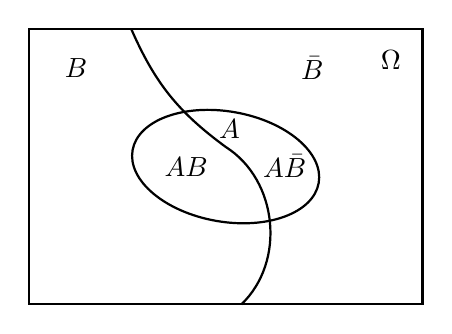
\begin{tikzpicture}[thick]
  \draw (0,0) rectangle (5,3.5);
  \node at (4.6,3.1) {$\Omega$};
  \node at (0.6,3) {$B$};
  \node at (3.6,3) {$\bar B$};
  \node at (2,1.75) {$AB$};
  \node at (3.25,1.75) {$A\bar B$};
  \node at (2.55,2.23) {$A$};
  \draw[rotate around={-10:(2.5,1.75)}]
    (2.5,1.75) ellipse (1.2 and 0.7);
  \draw (1.3,3.5) [bend right=15] to (2.5,2)
  [bend left=52] to (2.7,0);

\end{tikzpicture}
    \caption{用 $B$ 和 $\overline{B}$ 来分割样本空间}
  \end{minipage}
\end{figure}

\begin{example}[摸彩模型]
  设在 $n$ 张彩票中有一张奖券.
  求第二人摸到奖券的概率是多少?
\end{example}

\begin{solution}
  设 $A_i$ 表示事件“第 $i$ 人摸到奖券”,
  $i=1,2,\dotsc,n$,
  现在目的是求 $P(A_2)$.
  因为 $A_1$ 是否发生直接关系到 $A_2$ 发生的概率,
  即
  \[
    P(A_2 | A_1) = 0, \quad P(A_2 | A_1) = \frac{1}{n-1},
  \]
  而 $A_1$ 与 $\overline{A}_1$ 是两个概率大于 0 的事件:
  \[
    P(A_1) = \frac{1}{n}, \quad P(\overline{A}_1) = \frac{n-1}{n}.
  \]
  于是由全概率公式得
  \begin{align*}
    P(A_2)
    &= P(A_1) P(A_2 | A_1) + P(A_1) P(A_2 | \overline{A}_1)\\
    &= \frac{1}{n}.
  \end{align*}

  用类似的方法可得
  \[
    P(A_3) = P(A_4) = \dotsb = P(A_n) = \frac{1}{n}.
  \]

  如果设 $n$ 张彩票中有 $k(\le n)$ 张奖券,
  则可得
  \[
    P(A_1) = P(A_2) = \dotsb = P(A_n) = \frac{k}{n}.
  \]
  这说明,
  购买彩票时,
  不论先买后买,
  中彩机会是均等的.
\end{solution}

\begin{example}[敏感性问题调查]
  学生阅读黄色书刊和观看黄色影像会严重影响学生身心健康发展.
  但这些都是避着教师与家长进行的,
  属个人隐私行为.
  现在要设计一个调查方案,
  从调查数据中估计出学生中阅读黄色书刊和观看黄色影像的比率 $p$.
\end{example}

像这类敏感性问题的调查是社会调查的一类,
如一群人中参加赌博的比率、吸毒人的比率、经营者中偷税漏税户的比率、学生中考试作弊的比率等等.

敏感性问趣的调查方案,
关键要使被调查者愿意作出真实回答又能保守个人秘密.
一且调查方案设计有误,
被调查者就会拒绝配合,
所得调查数据将失去真实性.
经过多年研究和实践,
一些心理学家和统计学家设计了一种调查方案,
在这个方案中被调查者只需回答以下两个问题中的一个问题,
而且只需回答“是”或“否”.

\textbf{问题A}:
你的生日是否在7月1日之前?

\textbf{问题B}:
你是否看过黄色书刊或影像?

这个调查方来看似简单,
但为了消除被调查者的顾虑,
使被调查者确信他这次调查不会泄露个人秘密,
在操作上有以下关键点:
\begin{enumerate}
  \item 被调查者在没有旁人的情况下,
  独自一人回答问题.

  \item 被调查者从一个罐子中随机抽一只球,
  看过颜色后即放回.
  若抽到白球,
  则回答问题 A;
  若抽到红球,
  则回答问题 B.
  且罐中只有白球和红球.
\end{enumerate}

被调查者无论回答问题 A 或问题 B,
只需在下面答卷上认可的方框内打钩,
然后把答卷放入一只密封的投票箱内.

\begin{figure}
  \centering
  \begin{tikzpicture}[thick]
  \draw (0,0) rectangle (5,3.5);
  \node at (2.5,2.6) {答\,案};
  \node[draw ,rectangle] at (1.5,1.2) {};
  \node[draw ,rectangle] at (3.5,1.2) {};
  \node[left] at (1.5,1.2) {是};
  \node[left] at (3.5,1.2) {否};
\end{tikzpicture}
  \caption{敏感性问题的答卷}\label{fig1.4.4}
\end{figure}

如此的调查方法,
主要在于旁人无法知道被调查回答的是问题 A 还是问题 B,
由此可以极大地消除被调查者的顾虑.

现在的问题是如何分析调查的结果.
很显然,
我们对问题 A 是不感兴趣的.

首先我们设有 $n$ 张答卷 ($n$ 较大,
譬如 \num{1000} 以上),
其中有 $k$ 张回答“是”.
而我们又无法知道此 $n$ 张答卷中有多少张是回答问题 $B$ 的,
同样无法知道 $k$ 张回答“是”的答卷中有多少张是回答问题 $B$ 的.
但有两个信息我们是预先知道的,
即
\begin{enumerate}
  \item 在参加人数较多的场合,
  任选一人其生日在7月1日之前的概率为 0.5.

  \item 罐中红球的比率 $\pi$ 是已知.
  现在就要从这4个数据 $(n, k, 0.5, \pi)$ 去求出 $p$.
  因为由全概率公式得
  \[
    P(\text{是}) = P(\text{白球}) P(\text{是} | \text{白球})
    + P(\text{红球}) P(\text{是} | \text{红球}).
  \]
  所以将 $P(\text{红球}) = \pi$,
  $P(\text{白球}) = 1-\pi$,
  $P(\text{是} | \text{白球}) = 0.5$,
  $P(\text{是} | \text{红球}) = p$ 代入上式右边,
  而上式左边用频率 $k/n$ 代替,
  得
  \[
    \frac{k}{n} = 0.5 (1 - \pi) + p \cdot \pi.
  \]
  由此得
  \[
    p = \frac{k/n - 0.5(1 - \pi)}{\pi}
  \]
  因为我们用频率 $k/n$ 代替了概率 $P (\text{是})$,
  所以从上式得到的是 $p$ 的估计.
\end{enumerate}

例如,
在一次实际调查中,
罐中放有红球30个、白球20个,
则 $\pi = 0.6$,
调查结束后共收到 \num{1583} 张有效答卷,
其中有 389 张回答“是”,
由此可计算得
\[
  p = \frac{389/1583 - 0.5 \times 0.4}{0.6} = 0.0762.
\]
这表明:
约有 \SI{7.62}{\percent} 的学生看过黄色书刊或黄色影像.

\subsection{贝叶斯公式}

在乘法公式和全概率公式的基础上立即可推得一个很著名的公式.

\begin{property}[贝叶斯公式]\label{prop1.4.4}
  设 $B_1, B_2, \dotsc, B_n$ 是样本空间 $\Omega$ 的一个分割,
  即 $B_1, B_2, \dotsc, B_n$ 互不相容,
  且 $\bigcup_{i=1}^n B_i = \Omega$,
  如果 $P(A) > 0$, $P(B_i) > 0$, $i = 1,2, \dotsc, n$,
  则
  \begin{equation}
    P (B_i | A) = \frac{P(B_i) P(A|B_i)}{\sum_{j=1}^n P(B_j) P(A|B_j)},
    i = 1,2,\dotsc,n.
    \label{eq1.4.6}
  \end{equation}
\end{property}

\begin{proof}
  由条件概率的定义
  \[
    P(B_i|A) = \frac{P(AB_i)}{P(A)}.
  \]
  对上式的分子用乘法公式、分母用全概率公式,
  \begin{align*}
    & P(AB_i) = P(B_i) P(A|B_i),\\
    & P(A) = \sum_{j=1}^n P(B_j) P(A|B_j),
  \end{align*}
  即得
  \[
    P(B_i|A) = \frac{P(B_i) P(A|B_i)}{\sum_{j=1}^n P(B_j) P(A|B_j)}.
  \]
  结论得证.
\end{proof}

\begin{example}
  某地区居民的肝癌发病率为 \num{0.0004},
  现用甲胎蛋白法进行普查.
  医学研究表明,
  化验结果是存有错误的.
  已知患有肝癌的人其化验结果 \SI{99}{\percent} 呈阳性 (有病),
  而没患肝癌的人其化验结果 \SI{99.9}{\percent} 呈阴性 (无病).
  现某人的检查结果呈阳性,
  问他真的患肝癌的概率是多少?
\end{example}

\begin{solution}
  记 $B$ 为事件“被检查者患有肝癌”,
  $A$ 为事件“检查结果呈阳性”.
  由题设知
  \begin{gather*}
    P(B) = 0.0004, \quad P(\overline{B}) = 0.996,\\
    P(A|B) = 0.99, \quad P(A|\overline{B}) = 0.001.
  \end{gather*}

  我们现在的目的是求 $P(B|A)$.
  由贝叶斯公式得
  \begin{align*}
    P(B|A) &= \frac{P(B) P(A|B)}{P(B) P(A|B) + P(\overline{B}) P(A|\overline{B})}\\
    &= \frac{0.0004 \times 0.99}{0.0004 \times 0.99 + 0.9996 \times 0.001}\\
    &= 0.284.
  \end{align*}
  这表明,
  在检查结果呈阳性的人中,
  真患肝癌的人不到 \SI{30}{\percent},
  这个结果可能会使人吃惊,
  但仔细分析一下就可以理解了.
  因为肝癌发病率很低,
  在 \num{10000} 个人中,
  约有 4 人,
  而约有 \num{9996} 个人不惠肝癌.
  对 \num{10000} 个人用甲胎蛋白法进行检查,
  按其错检的概率可知,
  \num{9996} 个不患肝癌者中约有 $9996 \times 0.001 \cong 9.994$ 个呈阳性.
  另外 4 个真患肝癌者的检查报告中约有 $4 \times 0.99 \cong 3.96 $ 个呈阳性.
  仅从 \num{13.956} 个呈阳性者中看,
  真患肝癌的 3.96 人约占 \SI{28.4}{\percent}.
\end{solution}

进一步降低错检的概率是提高检验精度的关键.
在实际中由于技术和操作等种种原因,
降低错检的概率又是很困难的.
所以在实际中,
常采用复查的方法来减少错误率.
或用另一些简单易行的辅助方法先进行初查,
排除了大量明显不是肝癌的人后,
再用甲胎蛋白法对被怀疑的对象进行检查.
此时被怀疑的对象群体中,
肝癌的发病率已大大提高了.
警如,
对首次检查得阳性的人群再进行复查,
此时 $P(B) = 0.284$,
这时再用贝叶斯公式计算得
\[
  P(B|A) = \frac{0.284 \times 0.99}{0.284 \times 0.99 + 0.716 \times 0.0001} = 0.997.
\]
这就大大提高了甲胎蛋白法的准确率了.

在上面例中,
如果我们将事件 $B$ (“被检查者患有肝癌”) 看作是“原因”,
将事件 $A$ (“检查结果呈阳性”) 看作是最后“结果”.
则我们用贝叶斯公式在已知“结果”的条件下,
求出了“原因”的概率 $P(B|A)$.
而求“结果”的 (无条件) 概率 $P(A)$,
用全概率公式.
在上例中若取 $P(B) = 0.284$,
则
\begin{align*}
  P(A) &= P(B) P(A|B) + P(\overline{B}) P(A|\overline{B})\\
  &= 0.284 \times 0.99 + 0.716 \times 0.001\\
  &= 0.2819.
\end{align*}


条件概率的三公式中,
乘法公式是求事件交的概率.
全概率公式是求一个复杂事件的概率,
而贝叶斯公式是求一个条件概率.

在贝叶斯公式中,
如果称 $P(B_i)$ 为 $B_i$ 的先验概率,
称 $P(B_i |A)$ 为 $B_i$ 的后验概率, 则贝叶斯公式是专门用于计算后验概率的, 也就是通过$A$的发生这个新信息, 来对$B_i$的概率作出的修正. 下面例子很好地说明了这一点.

\begin{example}
  伊索寓言“孩子与狼”讲的是一个小孩每天到山上放羊,山里有狼出没.第一天,他在山上喊:“狼来了!狼来了!”,山下的村民闻声便去打狼,可到山上,发现狼没有来;第二天仍是如此;第三天,狼真的来了,可无论小孩怎么喊叫,也没有人来救他,因为前二次他说了谎,人们不再相信他了.
\end{example}

现在用贝叶斯公式来分析此寓言中村民对这个小孩的可信程度是如何下降的.

首先记事件$A$为“小孩说谎”,记事件$B$为“小孩可信”.不妨设村民过去对这个小孩的印象为
\begin{equation}\label{eq1.4.7}
  P(B) = 0.8,\quad P(\bar B) = 0.2.
\end{equation}

我们现在用贝叶斯公式来求$P(B|A)$,亦即这个小孩说了一次谎后,村民对他可信程度的改变.

在贝叶斯公式中我们要用到概率$P(A|B)$和$P(A|\bar B)$,这两个概率的含义是:前者为“可信”$(B)$的孩子“说谎”$(A)$的可能性,后者为“不可信”$(\bar B)$的孩子“说谎”$(A)$的可能性.在此不妨设
\[
  P(A|B) = 0.1,\quad P(A|\bar B) = 0.5.
\]

第一次村民上山打狼,发现狼没有来,即小孩说了谎$(A)$.村民根据这个信息,对这个小孩的可信程度改变为(用贝叶斯公式)
\begin{align*}
  P(B|A) & = \frac{P(B)P(A|B)}{P(B)P(A|B) + P(\bar B)P(A|\bar B) } \\
  & = \frac{0.8\times0.1}{0.8\times0.1 + 0.2\times0.5} = 0.444.
\end{align*}

这表明村民上了一次当后,对这个小孩的可信程度由原来的0.8调整为
0.444,也就是 \eqref{eq1.4.7} 调整为
\begin{equation}\label{eq1.4.8}
  P(B) = 0.444,\quad P(\bar B) = 0.556.
\end{equation}
在此基础上,我们再一次用贝叶斯公式来计算$P(B|A)$,亦即这个小孩第二次说谎后,村民对他的可信程度改变为
\[
  P(B|A) = \frac{0.444\times0.1}{0.444\times0.1 + 0.556\times0.5} = 0.138.
\]

这表明村民们经过两次上当,对这个小孩的可信程度已经从0.8下降到了
0.138,如此低的可信度,村民听到第三次呼叫时怎么再会上山打狼呢?

这个例子启发人们:若某人向银行贷款,连续两次未还,银行还会第三次贷款给他吗?
\begin{xiti}
  \item 某班级学生的考试成绩数学不及格的占15\%,语文不及格的占5\%,这两门都不及格的占3\%.
  \begin{enumerate}
    \item 已知一学生数学不及格,他语文也不及格的概率是多少?
    \item 已知一学生语文不及格,他数学也不及格的概率是多少?
  \end{enumerate}

  \item 设一批产品中一、二、三等品各占60\%,30\%,10\%.从中任意取出一件,结果不是三等品,求取到的是一等品的概率.

  \item 掷两颗骰子,以$A$记事件“两颗点数之和为10”,以$B$记事件“第一颗点数小于第二颗点数”,试求条件概率$P(A|B)$和$P(B|A)$.

  \item 设某种动物由出生活到10岁的概率为0.8,而活到15岁的概率为0.4.问现年为10岁的这种动物能活到15岁的概率是多少?

  \item 设10件产品中有4件不合格品,从中任取两件,已知其中一件是不合格品,求另一件也是不合格品的概率.

  \item 设$n$件产品中有$m$件不合格品,从中任取两件,已知两件中有一件是不合格品,求另一件也是不合格品的概率.

  \item 掷一颗骰子两次,以$x$,$y$分别表示先后掷出的点数,记
    \[
      A = \{ x + y = 10 \},\quad B = \{ x > y \},
    \]
    求$P(B|A),P(A|B)$.

  \item 已知$P(A)=1/4,P(B|A)=1/3,P(A|B)=1/2$,求$P(A\cup B)$.

  \item 已知$P(\bar A)=0.3,P(B)=0.4,P(A\bar B)=0.5$,求$P(B|A\cup \bar B)$.

  \item 设$A,B$为两事件,$P(A)=P(B)=1/3,P(A|B)=1/6$,求$P(\bar A|\bar B)$.

  \item 口袋中有1只白球,1只黑球.从中任取1只,若取出白球,则试验停止;若取出黑球,则把取出的黑球放回的同时,再加入1只黑球,如此下去,直到取出的是白球为止,试求下列事件的概率.
      \begin{enumerate}
        \item 取到第$n$次,试验没有结束;
        \item 取到第n次,试验恰好结束.
      \end{enumerate}

  \item 一盒晶体管中有6只合格品、4只不合格品.从中不返回地一只一只取出,试求第二次取出合格品的概率.

  \item 甲口袋有$a$只黑球、$b$只白球,乙口袋有$n$只黑球、$m$只白球.
      \begin{enumerate}
        \item 从甲口袋任取1只球放入乙口袋,然后再从乙口袋任取1只球.试求最后从乙口袋取出的是黑球的概率.
        \item 从甲口袋任取2只球放入乙口袋,然后再从乙口袋任取1只球.试求最后从乙口袋取出的是黑球的概率.
      \end{enumerate}

  \item 两台车床加工同样的零件,第一台出现不合格品的概率是0.03,第二台出现不合格品的概率是0.06,加工出来的零件放在一起,并且已知第一台加工的零件比第二台加工的零件多一倍.
      \begin{enumerate}
        \item 求任取一个零件是合格品的概率.
        \item 如果取出的零件是不合格品,求它是由第二台车床加工的概率.
      \end{enumerate}

  \item 已知男人中有5\%是色育患者,女人中有0.25\%是色盲患者,今从男女人数相等的人群中随机地挑选一人,发现恰好是色育患者,问此人是男性的概率是多少?

  \item 钥匙掉了,掉在宿舍里、掉在教室里、掉在路上的概率分别是40\%、30\%和20\%,而掉在上述三处地方被找到的概率分别是0.8、0.3和0.1.试求找到钥匙的概率.

  \item 口袋中有$a$个白球,$b$个黑球和$n$个红球,现从中一个一个不返回地取球.试证白球比黑球出现得早的概率为$a/(a+b)$,与$n$无关.

  \item 有两箱零件,第一箱装50件,其中10件是一等品;第二箱装30件,其中18件是一等品,现从两箱中随意挑出一箱,然而从该箱中任取两个零件,试求
      \begin{enumerate}
        \item 第一次取出的零件是一等品的概率;
        \item 在第一次取出的是一等品的条件下,第二次取出的零件仍然是一等品的概率.
      \end{enumerate}

  \item 学生在做一道有4个选项的单项选择题时,如果他不知道问题的正确答案时,就作随机猪测.现从卷面上看题是答对了,试在以下情况下求学生确实知道正确答案的概率.
      \begin{enumerate}
        \item 学生知道正确答案和胡乱猜测的概率都是$1/2$.
        \item 学生知道正确答案的概率是0.2.
      \end{enumerate}

  \item 口袋中有一只球,不知它的颜色是黑的还是白的.现再往口袋中放入一只白球,然后从口袋中任意取出一只,发现取出的是白球,试问口袋中原来那只球是白球的可能性为多少?

  \item 将$n$根绳子的$2n$个头任意两两相接,求恰好结成$n$个圈的概率.

  \item $m$个人相互传球,球从甲手中开始传出,每次传球时,传球者等可能地把球传给其余$m-1$个人中的任何一个.求第$n$次传球时仍由甲传出的概率.

  \item 甲、乙两人轮流掷一颗骰子,甲先掷.每当某人掷出1点时,则交给对方掷,否则此人继续掷.试求第$n$次由甲掷的概率.

  \item 甲口袋有1只黑球、2只白球,乙口袋有3只白球.每次从两口袋中各任取一球,交换后放人另一口袋.求交换$n$次后,黑球仍在甲口袋中的概率.

  \item 假设只考虑天气的两种情况:有雨或无雨.若已知今天的天气情况,明天天气保持不变的概率为$p$,变的概率为$1-p$.设第一天无雨,试求第$n$天也无雨的概率.

  \item 设罐中有$b$个黑球、$r$个红球,每次随机取出一个球,取出后将原球放回,再加人$c(>0)$个同色的球.试证:第$k$次取到黑球的概率为$b/(b+r),k=1,2,\cdots$.

  \item 设$P(A)>)$,试证
    \[
      P(B|A) \ge 1 - \frac{P(\bar B)}{P(A)}.
    \]

  \item 若事件$A$与$B$互不相容,且$P(\bar B)\ne0$,证明
    \[
      P(A|\bar B) = \frac{P(A)}{1-P(B)}.
    \]

  \item 设$A$,$B$为任意两个事件,且$A\subset B,P(B)>0$,则成立
    \[
      P(A) \le P(A|B).
    \]

  \item 若$P(A|B)>P(A|\bar B)$,试证$P(B|A)>P(B|\bar A)$.

  \item 设$P(A)=p,P(B)=1-\varepsilon$,证明
    \[
      \frac{p-\varepsilon}{1-\varepsilon} \le P(A|B) \le \frac p{1-\varepsilon}.
    \]
\end{xiti}


\section{独立性}

独立性是概率论中又一个重要概念,利用独立性可以简化概率的计算.下面先讨论两个事件之间的独立性,然后讨论多个事件之间的相互独立性,最后讨论试验之间的独立性.

\subsection{两个事件的独立性}
两个事件之间的独立性是指:一个事件的发生不影响另一个事件的发生.这在实际问题中是很多的,譬如在掷两颗骰子的试验中,记事件$A$为“第一颗骰子的点数为1”,记事件$B$为“第二颗骰子的点数为4”.则显然$A$与$B$的发生是相互不影响的.

另外,从概率的角度看,事件$A$的条件概率$P(A|B)$与无条件概率$P(A)$的差别在于:事件$B$的发生改变了事件$A$发生的概率,也即事件$B$对事件$A$有某种“影响”. 如果事件$B$的发生对事件A的发生毫无影响,即有$P(A|B)=P(A)$. 由此又可推出$P(B|A)=P(B)$,即事件$A$发生对$B$也无影响,可见独立性是相互的,它们都等价于

\begin{equation}\label{eq1.5.1}
  P(AB) = P(A)P(B).
\end{equation}
另外对$P(B)=0$,或$P(A)=0$,\eqref{eq1.5.1} 式仍然成立.为此,我们用 \eqref{eq1.5.1} 式作为两个事件相互独立的定义.

\begin{definition}{}{1.5.1}
  如果 \eqref{eq1.5.1} 式成立,则称事件$A$与$B$\textbf{相互独立}\index{D!独立性!相互独立},简称$A$与$B$独立,否则称$A$与$B$\textbf{不独立}\index{D!独立性!不独立}或\textbf{相依}.\index{D!独立性!相依}
\end{definition}

在许多实际问题中,两个事件相互独立大多是根据经验(相互有无影响)来判断的,如上述掷两颗骰子问题中A与B的独立性.但在有些问题中,有时也用  \eqref{eq1.5.1} 式来判断两个事件间的独立性.

\begin{example}[事件独立的例子]

  \begin{inparaenum}[(1)]
    \item 从一副52张的扑克牌中任取1张,以$A$记事件“取到黑桃”,以$B$记事件“取到爱司”,则因为$P(A)=1/4,P(B)=4/52=1/13$,而$AB$表示“取到黑桃爱司”,故$P(AB)=1/52$,所以$A$与$B$相互独立.

    \item\label{ex1.5.1.2} 考虑有三个小孩的家庭,并设所有8种情况
      \[
        bbb, bbg, bgb, gbb, bgg, gbg, ggb ,ggg
      \]
      是等可能的,其中$b$表示男孩,$g$表示女孩. 以$A$记事件“家中男女孩都有”,以$B$记事件“家中至多一个女孩”.则因为$P(A)=6/8,P(B)=4/8$,而$AB$表示“家中恰有一个女孩”,故$P(AB)=3/8$,所以$A$与$B$相互独立.

    \item 当考察的家庭有两个小孩时,样本空间只含4个样本点,它们是
      \[
        bb ,bg , gb ,gg
      \]

      若事件$A$、$B$仍如 (\ref{ex1.5.1.2}) 所设,则$P(A)=2/4,P(B)=3/4$,而$P(AB)=2/4$,由于$P(AB)\ne P(A)P(B)$,所以$A$与$B$不独立.
  \end{inparaenum}
\end{example}

\begin{property}\label{prop1.5.1}
  若事件$A$与$B$独立,则$A$与$\bar B$独立;$\bar A$与$B$独立;$\bar A$与$\bar B$独立.
\end{property}
\begin{proof}
  由概率的性质知
  \[
    P(A\bar B) = P(A) - P(AB).
  \]
  又由$A$与$B$的独立性知
  \[
    P(AB) = P(A)P(B),
  \]
  所以
  \[
    P(A\bar B) = P(A) - P(A)P(B) = P(A) [1 - P(B)] = P(A)P(\bar B).
  \]
  这表明$A$与$\bar B$独立. 类似可证$\bar A$与$\bar B$独立,$\bar A$ 与$B$独立.
\end{proof}

\subsection{多个事件的相互独立性}
首先研究三个事件的相互独立性,对此我们先给出以下的
\begin{definition}{}{1.5.2}
  设$A,B,C$是三个事件,如果有
  \begin{equation}\label{eq1.5.2}
    \left\{
      \begin{aligned}
        & P(AB) = P(A) P(B), \\
        & P(AC) = P(A) P(C), \\
        & P(BC) = P(B) P(C),
      \end{aligned}
    \right.
  \end{equation}
  则称$A,B,C$\textbf{两两独立}\index{D!独立性!两两独立}. 若还有
  \begin{equation}\label{eq1.5.3}
    P(ABC) = P(A) P(B) P(C),
  \end{equation}
  则称$A,B,C$\textbf{相互独立}.\index{D!独立性!相互独立}
\end{definition}

由此我们可以定义三个以上事件的相互独立性.
\begin{definition}{}{1.5.3}
  设有$n$个事件$A_1,A_2,\cdots,A_n$,对任意的$1\le i<j<k\cdots\le n$,如果以下等式均成立
  \begin{equation}\label{eq1.5.4}
    \left\{
      \begin{aligned}
        & P(A_iA_j) = P(A_i) P(A_j), \\
        & P(A_iA_jA_k) = P(A_i) P(A_j) P(A_k), \\
        & \vdots \\
        & P(A_1A_2\cdots A_n) = P(A_1)P(A_2) \cdots P(A_n),
      \end{aligned}
    \right.
  \end{equation}
  则称此$n$个事件$A_1,A_2,\cdots,A_n$\textbf{相互独立}.
\end{definition}

从上述定义可以看出,$n$个相互独立的事件中的任意一部分内仍是相互独立的,而且任意一部分与另一部分也是独立的.与性质 \ref{prop1.5.1} 类似,可以证明:将相互独立事件中的任一部分换为对立事件,所得的诸事件仍为相互独立的.

\begin{example}
  设$A$,$B$,$C$三事件相互独立,试证$A\cup B$与$C$相互独立.
\end{example}
\begin{proof}
  因为
  \begin{align*}
    P\big(\big(A\cup B)C) & = P(AC \cup BC) = P(AC) + P(BC) - P(ABC) \\
    & = P(A)P(C) + P(B)P(C) - P(A)P(B)P(C) \\
    & = [P(A) + P(B) - P(A)P(B)]P(C) =
    P(A \cup B) P(C),
  \end{align*}
  所以$A\cup B$与$C$相互独立.
\end{proof}

仿照此题的证明,可很容易推得:$AB$与$C$独立;$A-B$与$C$独立.

\begin{example}
  两射手彼此独立地向同一目标射击,设甲射中目标的概率为0.9,乙射中目标的概率为0.8,求目标被击中的概率是多少?
\end{example}
\begin{solution}
  记$A$为事件“甲射中目标”,$B$为事件“乙射中目标”. 注意到事件“目标被击中”$=A\cup B$,故
  \begin{align*}
    P(A\cup B) & = P(A) + P(B) - P(A)P(B) \\
    & = 0.9 + 0.8 - 0.9\times 0.8 = 0.98.
  \end{align*}
\end{solution}

\begin{example}
  某零件用两种工艺加工,第一种工艺有三道工序,各道工序出现不合格品的概率分别为$0.3,0.2,0.1$;第二章工艺有两道工序,各道工序出现不合格品的概率分别为$0.3,0.2$. 试问:
  \begin{enumerate}[label=(\arabic*)]
    \item 用哪种工艺加工得到合格品的概率较大些?
    \item 第二种工艺两道工序出现不合格品的概率都是0.3时,情况又如何?
  \end{enumerate}
\end{example}

\begin{solution}
  以$A_i$记事件“用第$i$种工艺加工得到合格品”,$i=1,2$.

  \begin{inparaenum}[(1)]
    \item 由于各道工序可看作是独立工作的,所以
    \begin{align*}
      & P(A_1) = 0.7\times 0.8 \times 0.9 = 0.504, \\
      & P(A_2) = 0.7\times 0.8 = 0.56,
    \end{align*}
    即第二种工艺得到合格品的概率较大些. 这个结果也是可以理解的,因为第二种工艺前两道工序出现不合格品的概率与第一种工艺相同,但少了一道工序,所以减少了出现不合格品的机会.

    \item 当第二种工艺两道工序出现不合格品的概率都是0.3时,
    \[
      P(A_2) = 0.7\times 0.7 = 0.49,
    \]
    即第一种工艺得到合格品的概率较大些.
  \end{inparaenum}
\end{solution}

\begin{example}
  有两名选手比赛射击,轮流对同一目标进行射击,甲命中目标的概率为$\alpha$,乙命中目标的概率为$\beta$.甲先射,谁先命中谁得胜.问甲、乙两人获胜的概率各为多少?
\end{example}
\begin{solution}
  记事件$A_i$为“第i次射击命中目标”,$i=1,2$,因为甲先射,所以事件“甲获胜”可以表示为
  \[
    A_1 \cup \bar A_1\bar A_2 A_3 \cup \bar A_1\bar A_2
    \bar A_3\bar A_4A_5\cup\cdots,
  \]
  又因为各次射击是独立的,所以得
  \begin{align*}
    P(\,\text{甲获胜}\,) & = \alpha + (1-\alpha)(1-\beta)\alpha + (1-\alpha)^2(1-\beta)^2\alpha + \cdots \\
    & = \alpha\sum_{i=0}^{+\infty}(1-\alpha)^i(1-\beta)^i \\
    & = \frac{\alpha}{1-(1-\alpha)(1-\beta)}.
  \end{align*}
  同理可得
  \begin{align*}
    P(\,\text{乙获胜}\,) & = P (\bar A_1A_2\cup \bar A_1\bar A_2\bar A_3A_4\cup\cdot) \\
    & = (1-\alpha)\beta + (1-\alpha)(1-\beta)(1-\alpha)\beta + \cdots \\
    & \beta (1-\alpha)\sum_{i=0}^{+\infty}(1-\alpha)^i(1-\beta)^i \\
    & = \frac{\beta(1-\alpha)}{1-(1-\alpha)(1-\beta)}.
  \end{align*}
\end{solution}

此题在等比级数求和时,应该有条件:公比$|(1-\alpha)(1-\beta)|M1$. 这一点不难从题目的实际意义中得到. 因为对本题而言,$\alpha,\beta$取值为零或1均是无意义的.

\begin{example}
  系统由多个元件组成,且所有元件都独立地工作.设每个元件正常工作的概率都为$p=0.9$,试求以下系统正常工作的概率.
  \begin{enumerate}[label=(\arabic*)]
    \item 串联系统$S_1$: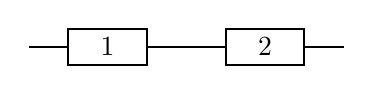
\begin{tikzpicture}[baseline=(a.base),thick]
                       \draw (0,0) -- (4,0);
                       \node(a)[minimum width=1cm,minimum height=0.4cm,draw,fill=white] at (1,0){1};
                       \node[minimum width=1cm,minimum height=0.4cm,draw,fill=white] at (3,0){2};
                    \end{tikzpicture}.
    \item 并联系统$S_2$: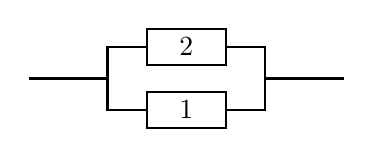
\begin{tikzpicture}[baseline=(a.base),thick,
     every node/.style =
     { minimum width=1cm,minimum height=0.4cm,draw,fill=white}]
     \node[draw = white](a) at (2,0) {};
     \draw (0,0) -- (1,0)  (3,0) -- (4,0)
         (1.5,-0.4) -- (1,-0.4) -- (1,0.4) -- (1.5,0.4)
          (2.5,-0.4) -- (3,-0.4) -- (3,0.4) -- (2.5,0.4);
     \node at (2,-0.4) {1} ;
     \node at (2,0.4) {2} ;
   \end{tikzpicture}.
   \item 5个元件组成的桥式系统$S_3$: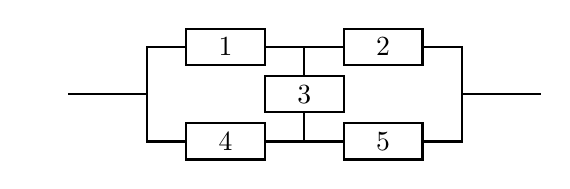
\begin{tikzpicture}[baseline=(a.base),thick,
  every node/.style =
   { minimum width=1cm,minimum height=0.4cm,draw,fill=white}]
   \node[draw = white] (a) at (0,0) {};
   \draw (0,0) -- (1,0) (3,-0.6) -- (3,0.6) (5,0) -- (6,0)
         (1,0.6) -- (1,-0.6) -- (5,-0.6) -- (5,0.6) -- cycle;
   \node at (2,-0.6) {4};
   \node at (2,0.6) {1};
   \node at (3,0) {3};
   \node at (4,0.6) {2};
   \node at (4,-0.6) {5};
\end{tikzpicture}.
  \end{enumerate}
\end{example}

\begin{solution}
  设$S_i=$“第$i$个系统正常工作”,$A_i=$“第$i$个元件正常工作”.

  \begin{inparaenum}[(1)]
    \item 对申联系统而言,“系统正常工作”相当于“所有元件正常工作”,即$S_1=A_1A_2$,所以
        \[
          P(S_1) = P(A_1A_2) = P(A_1)P(A_2) = p^2 = 0.81.
        \]

        这也可看出:两个正常工作概率为0.9的元件组成的串联系统,其系统正常工作的概率下降为0.81.

    \item 对并联系统而言,“系统正常工作”相当于“至少一个元件正常工作”,即$S_2=A_1\cup A_2$,所以
        \begin{align*}
          P(S_2) & P(A_1\cup A_2) = P(A_1) + P(A_2) - P(A_1A_2) \\
          & = p + p - p^2 = 0.99.
        \end{align*}
        或
        \begin{align*}
          P(S_2) & = 1 - P(\bar S_2) = 1 - P(\bar{A_1\cup A_2}) = 1 - P(\bar A_1\cap \bar A_2) \\
          & = 1 - P(\bar A_1)P(\bar A_2) = 1 - (1-p)^2 = 0.99.
        \end{align*}
        这也可看出:两个正常工作概率为0.9的元件组成的并联系统,其系统正常工作的概率提高至0.99.

        \item 在桥式系统中,第3个元件是关键,我们先用全概率公式得
        \[
          P(S_3) = P(A_3)P(S_3|A_3) + P(\bar A_3)P(S_3|\bar A_3).
        \]
        因为在“第3个元件正常工作”的条件下,系统成为先并后串系统(见图 \ref{fig1.5.1}). 所以
        \begin{align*}
          P(S_3|A_3) & = P\big( ( A_1\cup A_4 )
          (A_2 \cup A_5) \big) = P(A_1\cup A_4)P(A_2\cup A_5) \\
          & = [ 1 - (1-p)^2 ]^2 = 0.9801.
        \end{align*}

        又因为在“第3个元件不正常工作”的条件下,系统成为先串后并系统(见图 \ref{fig1.5.2}).
  \end{inparaenum}
  \begin{figure}[!ht]
    \centering
    \begin{minipage}{0.48\linewidth}
      \centering
      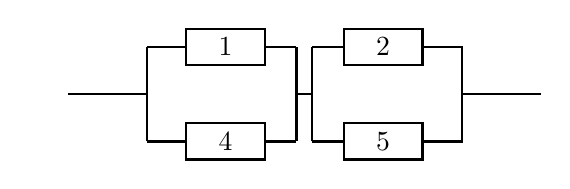
\begin{tikzpicture}[baseline=(a.base),thick,
  every node/.style =
   { minimum width=1cm,minimum height=0.4cm,draw,fill=white}]
   \node[draw = white] (a) at (0,0) {};
   \draw (0,0) -- (1,0) (2.9,0) -- (3.1,0)
    (5,0) -- (6,0) (2.9,-0.6) -- (2.9,0.6)
    (3.1,-0.6) -- (3.1,0.6)
         (1,0.6) -- (1,-0.6)(2.9,-0.6) (3.1,-0.6)-- (5,-0.6) -- (5,0.6) -- (3.1,0.6) (2.9,0.6) -- cycle;
    \draw (1,0.6) -- (2.9,0.6) (1,-0.6) -- (2.9,-0.6);
   \node at (2,-0.6) {4};
   \node at (2,0.6) {1};
   \node at (4,0.6) {2};
   \node at (4,-0.6) {5};
   \end{tikzpicture}
   \caption{先并后串系统\label{fig1.5.1}}
    \end{minipage}%
    \begin{minipage}{0.48\linewidth}
      \centering
      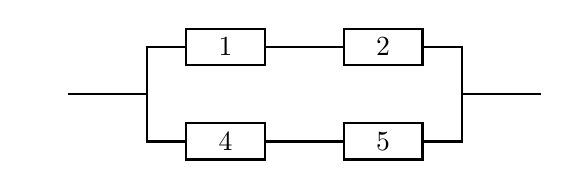
\begin{tikzpicture}[baseline=(a.base),thick,
  every node/.style =
   { minimum width=1cm,minimum height=0.4cm,draw,fill=white}]
   \node[draw = white] (a) at (0,0) {};
   \draw (0,0) -- (1,0)  (5,0) -- (6,0)
         (1,0.6) -- (1,-0.6) -- (5,-0.6) -- (5,0.6) -- cycle;
   \node at (2,-0.6) {4};
   \node at (2,0.6) {1};
   \node at (4,0.6) {2};
   \node at (4,-0.6) {5};
\end{tikzpicture}
   \caption{先串后并系统\label{fig1.5.2}}
    \end{minipage}
  \end{figure}
  所以
  \[
    P(S_3|\bar A_3) = P(A_1A_2|\cup A_4A_5) = 1 - (1-p^2)^2 = 0.9639.
  \]
  最后我们得
  \begin{align*}
    P(S_3) & = p [ 1-(1-p)^2 ]^2 + (1-p)[ 1-(1-p^2)^2 ] \\
    & = 0.9\times 0.9801 + 0.1 \times 0.9639 = 0.9785.
  \end{align*}
\end{solution}

\subsection{试验的独立性}
利用事件的独立性可以定义两个或更多个试验的独立性.

\begin{definition}{}{1.5.4}
  设有两个试验$E_1$和$E_2$,假如试验$E_1$的任一结果(事件)与试验$E_2$的任一结果(事件)都是相互独立的事件,则称\textbf{这两个试验相互独立}.
\end{definition}

例如掷一枚硬币(试验$E_1$)与掷一颗骰子(试验$E_2$)是相互独立的试验.

类似地可以定义$n$个试验$E_1,E_2,\cdots,E_n$的相互独立性:如果$E_1$的任一结果、$E_2$的任一结果$\cdots\cdots E_n$的任一结果都是相互独立的事件,则称\textbf{试验$E_1,E_2,\cdots,E_n$相互独立}. 如果这$n$个独立试验还是相同的,则称其为\textbf{$n$重独立重复试验}. 如果在$n$重独立重复试验中,每次试验的可能结果为两个:$A$或$\bar A$,则称这种试验为\textbf{$n$重伯努利试验}. \index{B!伯努利试验}

例如掷$n$枚硬币、掷$n$颗骰子、检查$n$个产品等,都是$n$重独立重复试验.

\begin{example}
  某彩票每周开奖一次,每次提供十万分之一的中奖机会,且各周开奖是相互独立的.若你每周买一张彩票,尽管你坚持十年(每年52周)之久,你从未中奖的可能性是多少?
\end{example}

\begin{solution}
  按假设,每次中奖的可能性是$10^{-5}$,于是每次不中奖的可能性是$1-10^{-5}$. 另外,十年中你共购买彩票520次,每次开奖都是相互独立的,相当于进行了520次独立重复试验.记$A_i$为“第$i$次开奖不中奖”,$i=1,2,\cdots,520$,则$A_1,A_2,\cdots,A_{520}$相互独立,由此得十年中你从未中奖的可能性是
  \[
    P(A_1A_2\cdots A_{520}) = (1 - 10^{-5})^{520} =  0.9948.
  \]
  这个概率表明十年中你从未中奖是很正常的事.
\end{solution}

如果将上例中每次中奖机会改成“万分之一”,则十年中从未中奖的可能性还是很大的,为0.9493.

\begin{xiti}
  \item 三人独立地破译一个密码,他们能单独译出的概率分别为$1/5$,$1/3$,$1/4$,求此密码被译出的概率.

  \item 有甲乙两批种子,发芽率分别为0.8和0.7,在两批种子中各任取一粒,求:
      \begin{enumerate}
        \item 两粒种子都能发芽的概率;
        \item 至少有一粒种子能发芽的概率;
        \item 恰好有一粒种子能发芽的概率.
      \end{enumerate}

  \item 甲、乙两人独立地对同一目标射击一次,其命中率分别为0.6和0.7,现已知目标被击中,求它是甲射中的概率.

  \item 设电路由$A$,$B$,$C$三个元件组成,若元件$A$,$B$,$C$发生故障的概率分别是0.3,0.2,0.2,且各元件独立工作,试在以下情况下,求此电路发生故障的概率:
      \begin{enumerate}
        \item $A$,$B$,$C$三个元件串联;
        \item $A$,$B$,$C$三个元件并联;
        \item 元件$A$与两个并联的元件$B$及$C$串联而成.
      \end{enumerate}

  \item 在一小时内甲,乙,丙三台机床需维修的概率分别是0.9,0.8和0.85,求一小时内
      \begin{enumerate}
        \item 没有一台机床需要维修的概率;
        \item 至少有一台机床不需要维修的概率;
        \item 至多只有一台机床需要维修的概率.
      \end{enumerate}

  \item 设$A_1,A_2,A_3$相互独立,且$P(A_i)=1/3,i=1,2,3$. 试求$A_1,A_2,A_3$中
      \begin{enumerate}
        \item 至少出现一个的概率;
        \item 恰好出现一个的概率;
        \item 最多出现一个的概率.
      \end{enumerate}

  \item 若事件$A$与$B$相互独立且互不相容,试求$\min\{P(A),P(B)\}$.

  \item 假设$P(A)=0.4,P(A\cup B)=0.7$,在以下情况下求$P(B)$:
      \begin{enumerate}
        \item $A,B$互不相容;
        \item $A,B$独立;
        \item $A\subset B$.
      \end{enumerate}

  \item 设$A,B,C$两两独立,且$ABC=\varnothing$.
      \begin{enumerate}
        \item 如果$P(A)=P(B)=P(C)=x$,试求$x$的最大值;
        \item 如果$P(A)=P(B)=P(C)<1/2$,且$P(A\cup B\cup C)=9/16$,求$P(A)$.
      \end{enumerate}

  \item 事件$A,B$独立,两个事件仅$A$发生的概率或仅$B$发生的概率都是$1/4$,求$P(A)$及$P(B)$.

  \item 一实习生用同一台机器接连独立地制造3个同种零件,第$i$个零件是不合格品的概率为$p_i=1/(i+1),i=1,2,3$,以$X$表示3个零件中合格品的个数,求$P(X=2)$.

  \item 同时抛掷3枚均匀的硬币,试求恰好有两枚正面向上的概率.

  \item 一射手对同一目标独立地进行四次射击,若至少命中一次的概率为80/81,试求该射手进行-一次射击的命中率.

  \item 每次射击命中率为0.2,试求:射击多少次才能使至少击中一次的概率不小于0.9?

  \item 设猎人在猎物100米处对猎物打第一枪,命中猎物的概率为0.5.若第一枪未命中,则猎人继续打第二枪,此时猎物与猎人已相距150米.若第二枪仍未命中,则猎人继续打第三枪,此时猎物与猎人已相距200米.若第三枪还未命中,则猎物逃逸.假如该猎人命中猎物的概率与距离成反比,试求该猎物被击中的概率.

  \item 已知某商场一天内来$k$个顾客的概率为$\lambda^k\ee^{-\lambda}/k!,k=0,1,\cdots$,其中$\lambda>0$. 又设每个到达商场的顾客购买商品是独立的,其概率为$p$,试证:这个商场一天内有$r$个顾客购买商品的概率为:$(\lambda p)^r\ee^{-\lambda p}/r!$.

  \item 一个人的血型为$A$,$A$,$AB$,$O$型的概率分别为0.37,0.21,0.08,0.34.现任意挑选四个人,试求:
      \begin{enumerate}
        \item 此四人的血型全不相同的概率;
        \item 此四人的血型全部相同的概率.
      \end{enumerate}

  \item 甲、乙两选手进行乓球单打比赛,已知在每局中甲胜的概率为0.6,乙胜的概率为0.4. 比赛可采用三局二胜制或五局三胜制,问哪一种比赛制度对甲更有利?

  \item 甲、乙、丙三人进行比赛,规定每局两个人比赛,胜者与第三人比赛,依次循环,直至有一人连胜两次为止,此人即为冠军.而每次比赛双方取胜的概率都是1/2,现假定甲、乙两人先比,试求各人得冠军的概率.

  \item 甲、乙两个赌徒在每一局获胜的概率都是1/2.两人约定谁先赢得一定的局数就获得全部赌本.但赌博在中途被打断了,请问在以下各种情况下,应如何合理分配赌本:
      \begin{enumerate}
        \item 甲、乙两个赌徒都各需赢$k$局才能获胜;
        \item 甲赌徒还需赢2局才能获胜,乙赌徒还需赢3局才能获胜;
        \item 甲赌徒还需赢$n$局才能获胜,乙赌徒还需赢$m$局才能获胜.
      \end{enumerate}

  \item 试证:概率为零的事件与任何事件都是独立的.

  \item 设$A,B,C$三事件相互独立,试证$A-B$与$C$独立.

  \item 设$0<P(B)<1$,试证事件$A$与$B$独立的充要条件是
  \[
    P(A|B) = P(A|\bar B).
  \]

  \item 设$0<P(A)<1,0<P(B)<1,P(A|B)+P(\bar A|\bar B)=1$,试证$A$与$B$独立.

  \item 若$P(A)>0,P(B)>)$,如果$A,B$相互独立,试证$A,B$相容.
\end{xiti} 

% !TeX root = main.tex
% Edit by: CamuseCao
\setcounter{chapter}{1}
\chapter{随机变量及其分布}

为了进行定量的数学处理,必须把随机现象的结果数量化.这就是引进随机变量的原因随机变量的引进使得对随机现象的处理更简单与直接,也更统一而有力.本章我们将主要讨论一维随机变量及其分布.

\section{随机变量及其分布}

在第一章中我们曾提及随机变量,在那里我们把“用来表示随机现象结果的变量“称为随机变量,其中“表示”一词的含义是什么?这是要进一步探讨的问题.

\subsection{随机变量的概念}

在随机现象中有很多样本点本身就是用数量表示的,由于样本点出现的随机性,其数量呈现为随机变量,譬如

\begin{itemize}
	\item 掷一颗散子,出现的点数$X$是一个随机变量.
	\item 每天进入某超市的顾客数$Y$;顾客购买商品的件数 $U$;顾客排队等候付款的时间 $V,Y,LU,V$ 是三个不同的随机变量,
	\item 电视机的寿命$T$是一个随机变量.
	\item 测量的误差 $\varepsilon $ 是一个随机变量.
\end{itemize}

在随机现象中还有不少样本点本身不是数,这时可根据研究需要设计随机变量,譬如
\begin{itemize}
	\item 检查一个产品,只考察其合格与否,则其样本空间为$\Omega=\{$合格品,不合格品$\}$, 这时可设计一个随机变量 $X$ 如下:
\end{itemize}

\begin{table}[htbp]
	\centering
	\begin{tabular}{ccc}
		样本点   &       & $X$的取值 \\\hline
		合格品   &   $ \longrightarrow $ & 0 \\
		不合格品 &    $ \longrightarrow $ & 1 \\
	\end{tabular}%
\end{table}%

在此可将 $ X $ 解释为“检查一个产品中不合格品数”.若此种产品的不合格品率为$ p $,则$ X $取各种值的概率可列表如下:

\begin{table}[htbp]
	\centering
	\begin{tabular}{c|cc}
		$ X $     & $ 0 $     & $ 1 $ \\\hline
		$ P $     & $ 1-p $   & $ p $ \\
	\end{tabular}%
\end{table}%


\begin{itemize}
	\item 检查三个产品,则有8个样本点,若记$X$为“三个产品中的不合格品数”,则$ X $与样本点之间有如下对应关系:
\end{itemize}

\begin{table}[htbp]
	\centering
	\begin{tabular}{ccc}
		样本点   &       & $ X $的取值 \\\hline
		$ \omega_1=(0,0,0) $ &   $ \longrightarrow $    & 0 \\
		$ \omega_2=(1,0,0) $ &   $ \longrightarrow $    & 1 \\
		$ \omega_3=(0,1,0) $ &   $ \longrightarrow $    & 1 \\
		$ \omega_4=(0,0,1) $ &   $ \longrightarrow $    & 1 \\
		$ \omega_5=(0,1,1) $ &   $ \longrightarrow $    & 2 \\
		$ \omega_6=(1,0,1) $ &   $ \longrightarrow $    & 2 \\
		$ \omega_7=(1,1,0) $ &   $ \longrightarrow $    & 2 \\
		$ \omega_8=(1,1,1) $ &   $ \longrightarrow $    & 3 \\
	\end{tabular}%
\end{table}%

这样$ X $取各种值就是如下的互不相容的事件:

\begin{equation}
\begin{array}{ll}
{ \{ X=0 \}=\{\omega_{1}\} ;} & \{  X=1 \}=\{\omega_{2}, \omega_{3}, \omega_{4} \}; \\
{ \{ X=2 \}=\{\omega_{5}, \omega_{6}, \omega_{7}\}};\quad &{\{ X=3\}=\{ \omega_{8} \}}.
\end{array}
\end{equation}

若此种产品的不合格品率为$ p $,则$ X $取各种值的概率可列表如下:

\[
\begin{array}{c|cccc}{x} & {0} & {1} & {2} & {3} \\ \hline P & {(1-p)^{3}} & {3 p(1-p)^{2}} & {3 p^{2}(1-p)} & {p^{3}}\end{array}
\]

\begin{definition}{}{}
	定义在样本空间$\Omega$上的实值函数$ X=X(\omega) $称为\textbf{随机变量}, \index{S!随机变量}常用大写字母$ X,Y,Z $等表示随机变量,其取值用小写字母$ x,y,z$等表示.假如一个随机变量仅取有限个或可列个值,则称其为\textbf{离散随机变量}. \index{S!随机变量!离散随机变量}假如一个随机变量的可能取值充满数轴上的一个区间$ (a,b) $, 则称其为\textbf{连续随机变量}, \index{S!随机变量!连续随机变量}其中$ a $可以是$ -\infty ,b $可以是$ +\infty $.
\end{definition}


这个定义表明:随机变量$ X $是样本点$ \omega $的一个函数,这个函数可以是不同样本点对应不同的实数,也允许多个样本点对应同一个实数.这个函数的自变量(样本点)可以是数,也可以不是数,但因变量一定是实数.

与微积分中的变量不同,概率论中的随机变量$ X $是一种“随机取值的变量”.以认识离散随机变例,我们不仅要知道$ Y $取哪些值,而且还要知道它取这些值的概率各是多少,这就需要分布的概念.有没有分布是区分一般变量与随机变量的主要标志.

\subsection{随机变量的分布函数}

随机变量$ X $是样个点$ \omega $的一个值函数.若$ B $是某些实数组成的集合,即$ B\subset \MR , \MR $表示实数集、则$ X\in B $表示如下的随机事件

\[
\{\omega: X(\omega)\in B\} \subset \Omega
\]

这就是我们可以用随性变立量得某些取值来表示随机事件的依据.臂如

\begin{itemize}
	\item 记$ X $表示掷一颗骰子出现的点数,明$ X $的可能取值为$ 1,2,\cdots ,6 $.这是一个离散随机变量.事件$A=$“点数小于等于3”,可以表示为$ A=\{X\leq 3\} $.
	\item 记$ Y $表示一天内到达某商场的顾客数.则$ Y $的可能取值为$ 0,1,2\dotsc ,n\dotsc $这也是一个离散随机变量.事件$B=$“至少来1000位顾客”,可以表示为$ B=\{ X\geq 1000 \} $.
	\item 记$ T $表示某电器品的使目寿命,则$T$的可能取值充满区间$ [0,+o\infty ) $.这楚一个连续随机变量.事件$C=$“使用寿命在40000至50000小时之间”,可以表示为$ C=\{ 40000 \le T\le 50000 \} $.
\end{itemize}



为了掌握$ X $的统计规律性,我们只要掌握$ X $取各种值的概率.由于

\[
\{a < X \leq b \} = \{ X \leq b\} - \{x\leq a\},
\]

因此只要对任意实数$ x $,知道了件$ X\geq x $的概率就够了,这个概率具有累积特性,常用$ F $表示.另外这个概率与$ x $有关,不同的$ x $,此累积概率的值也不同,为此记

\[
  F(x) = P(X\leq x),
\]

于是$ F(x) $所有$ x\in(-\infty,+\infty) $都有定义,而$ F(x) $是定义在$ (\infty,+\infty ) $上、取值于$ [0,1] $的一个函数.这就是我们下面要引入的分布函数.

\begin{definition}{}{}
	设$ X $是一个随机变量,对任意实数$ x $,称
	\begin{equation}
	F(x)=P(X \leqslant x) \label{2.1.1}
	\end{equation}
	为随机变量$ X $的\textbf{分布函数}\index{S!随机变量!分布函数}.且称$ X $服从$ F(x) $,记为$ X\sim F(x) $.有时也可用$F_{X}(x)$以表明是$ X $的分布函数(把$ X $作为$ F $的下标).
\end{definition}

\begin{example}
	向半径为$ r $的圆内随机抛一点,求此点到圆心之距离$ X $的分布函数$ F(x) $,并求$P\left(X>\frac{2 r}{3}\right)$.
\end{example}

\begin{solution}
	事件“$ X\le x $”表示所抛之点落在半径为$x(0 \leqslant x \leqslant r)$的圆内,故由几何概率知
	
	\[
	F(x)=P(X \leqslant x)=\frac{\pi x^{2}}{\pi r^{2}}=\left(\frac{x}{r}\right)^{2},
	\]
	
	从而
	
	\[
	P\left(X>\frac{2 r}{3}\right)=1-P\left(X \leqslant \frac{2 r}{3}\right)=1-\left(\frac{2}{3}\right)^{2}=\frac{5}{9}.
	\]
\end{solution}
	



从分布函数的定义可见,任一随机变量$ X $(离散的或连续的)都有一个分布函数.有了分布函数,就可据此算得与随机变量$ X $有关事件的概率.下面先证明分布函数的三个基本性质.

\begin{theorem}{}{}
	任一分布函数$F(x)$都具有如下三条基本性质:
	\begin{enumerate}
		\item \textbf{单调性} $ F(x) $是定义在整个实数轴$ (-\infty,+\infty ) $上的单调非减函数,即对任意的$ x_1<x_2 $,有$ F(x_1)\leq F(x_2) $.
		\item 有界性对任意的$ x $,有$ 0\leq F(x)\leq 1 $,且
		\[
		\begin{array}{l}{F(-\infty)=\lim _{x \rightarrow-\infty} F(x)=0}, \\ {F(+\infty)=\lim _{x \rightarrow+\infty} F(x)=1}.\end{array}
		\]
		
		\item 右连续性$ F(x) $是$ x $的右连续函数,即对任意的$ x_0 $,有
		\[
		\lim _{x \rightarrow x_{0}+} F(x)=F\left(x_{0}\right),
		\]
		即
		\[
		F\left(x_{0}+0\right)=F\left(x_{0}\right)
		\]
	\end{enumerate}
\end{theorem}

\begin{proof}
	(1)是显然的,下证(2).由于$ F(x) $是事件$\{X \leqslant x\}$的概率,所以$ 0\leq
	F(x)\leq 1 $.由$ F(x) $的单调性知,对任意整数$ m $和$ n $,有
	
	\[
	\lim _{x \rightarrow-\infty} F(x)=\lim _{m \rightarrow-\infty} F(m), \lim _{x \rightarrow+\infty} F(x)=\lim _{n \rightarrow+\infty} F(n)
	\]
	
	都存在.又由概率的可列可加性得
	
	
  \begin{align*}
    1 & = P(-\infty<X<+\infty) = P\left(\bigcup_{i=-\infty}^{+\infty}\{i-1<X \leqslant i\}\right) \\ & = \sum_{i=-\infty}^{+\infty} P(i-1<X \leqslant i)=\lim _{n \rightarrow+\infty \atop m \rightarrow-\infty} \sum_{i =m}^{n} P(i-1<X \leqslant i) \\
    &=\lim _{n \rightarrow+\infty} F(n)-\lim _{m \rightarrow-\infty} F(m)
  \end{align*}

	
	再证(3),因为$ F(x) $是单调有界非降函数,所以其任一点$ x_0 $的右极限$ F(x_0+0) $必存在.为证右连续性,只要对单调下降的数列$x_{1}>x_{2}>\cdots>x_{n}>\cdots>x_{0}$,当$x_{n} \rightarrow x_{0}(n \rightarrow+\infty)$时,证明$\lim _{n \rightarrow+\infty} F\left(x_{n}\right)=F\left(x_{0}\right)$成立即可.因为
	
	\begin{align*}
	F\left(x_{1}\right)-F\left(x_{0}\right) & =P\left(x_{0}<X \leqslant x_{1}\right)=P\left(\bigcup_{r=1}^{+\infty}\left\{x_{i+1}<X \leqslant x_{i}\right\}\right) \\
	&=\sum_{i=1}^{+\infty} P\left(x_{i+1}<X \leqslant x_{i}\right)=\sum_{i=1}^{+\infty}\left[F\left(x_{i}\right)-F\left(x_{t+1}\right)\right] \\
	&=\lim _{n \rightarrow \infty}\left[F\left(x_{1}\right)-F\left(x_{n}\right)\right]=F\left(x_{1}\right)-\lim _{n \rightarrow \infty} F\left(x_{n}\right)
	\end{align*}
\end{proof}

由此得

\[
F\left(x_{0}\right)=\lim _{x \rightarrow+\infty} F\left(x_{n}\right)=F\left(x_{0}+0\right)
\]

至此三条基本性质全部证得.

以上三条基本性质是分布函数必须具有的性质,还可以证明:满足这三个基本性质的函数一定是某个随机变量的分布函数.从而这三个基本性质成为判别某个函数是否能成为分布函数的充要条件.

有了随机变量$ X $的分布函数,那么有关$ X $的各种事件的概率都能方便地用分布函数来表示了,例如,对任意的实数$ a $与$ b $,有

\begin{align*}
  &P(a<X \leqslant b) = F(b)-F(a),\\
  &P(X=a) = F(a)-F(a-0), \\
  &P(X \geqslant b) = 1-F(b-0), \\
  &P(X>b) = 1-F(b), \\
  &P(a<x<b) = F(b-0)-F(a), \\
  &P(a \leqslant X \leqslant b) = F(b)-F(a-0), \\
  &P(a \leqslant X<b) = F(b-0)-F(a-0).
\end{align*}

特别当$ F(x) $在$ a $与$ b $处连续时,有

\[
F(a-0)=F\langle a), \quad F(b-0)=F(b).
\]

这些公式将会在今后的概率计算中经常遇到.

\begin{example}
	设有一反正切函数
	\[
	F(x)=\frac{1}{\pi}\left[\arctan x+\frac{\pi}{2}\right], \quad-\infty<x<+\infty
	\]
	
	它在整个数轴上是连续、单调严增函数,且$F(+\infty)=1, F(-\infty)=0$.由于此$ F(x) $满足分布函数的三个基本性质,故$ F(x) $是一个分布函数.称这个分布函数为柯西分布函数,其图形见图~\ref{fig:2-1-1}.
	
	\begin{figure}[!ht]
  \centering
\begin{tikzpicture}[>=Stealth,xscale=1.3,yscale=2,semithick]
\draw[->](-2,0)--(0,0)node[below left]{$O$}--(2,0)node[below]{$x$};
\draw[->](0,-0.5)--(0,1.3)node[left]{$F(x)$};
\draw[dashed](-2,1)--(2,1)(1,0)node[below]{$1$}--(1,0.75)--(0,0.75)node[left]{$F(1)$}
(-1,0)node[below]{$-1$}--(-1,0.25)--(0,0.25)node[right]{$F(-1)$};
\draw[thick,domain=-2:2,samples=100]plot(\x,{(atan(\x))/180+0.5});
\end{tikzpicture}
  \caption{柯西分布函数}\label{fig:2-1-1}
\end{figure}
	
	若$X$服从柯西分布,则
	
	\[
	\begin{aligned} P(-1 \leqslant X \leqslant 1) &=F(1)-F(-1) \\ &=\frac{1}{\pi}[\arctan (1)-\arctan (-1)] \\ &=\frac{1}{\pi}\left[\frac{\pi}{4}-\left(-\frac{\pi}{4}\right)\right]=\frac{1}{2} \end{aligned}
	\]
	
\end{example}

\subsection{离散随机变量的概率分布列}

对离散随机变量而言,常用以下定义的分布列来表示其分布.

\begin{definition}{}{}
	设$ X $是一个离散随机变量,如果$ X $的所有可能取值是$ x_1,x_{2}, \cdots, x_{n}, \cdots$ 则称$ X $取$ x_i $, 的概率
	\begin{equation}
	p_{i}=p\left(x_{i}\right)=P\left(X=x_{i}\right), i=1,2, \cdots, n, \cdots \label{eq:2.1.2}
	\end{equation}
	
	为$ X $的概率分布列或简称为分布列,记为$X \sim\left|p_{t}\right|$,分布列也可用如下列表方式来表示:
	
	\[
	\begin{array}{c|ccccc}
	X	&    x_{1}     &    x_{2}     &    \cdots     &     x_{n}    &   \cdots \\ \hline
	P	&    p(x_1)     &    p(x_2)     &    \cdots     &    p(x_n)     &   \cdots \\
	\end{array}
	\]
	
	
	或记成
	
	\[
	\left( \begin{array}{ccccc}{x_{1}} & {x_{2}} & {\cdots} & {x_{n}} & {\cdots} \\ {p\left(x_{1}\right)} & {p\left(x_{2}\right)} & {\cdots} & {p\left(x_{n}\right)} & {\cdots}\end{array}\right]
	\]
	
\end{definition}


第一章中我们已见过多个分布列,不同的离散随机变量可能有不同的分布列,甚至在一个样本空间上可以定义几个服从不同分布列的随机变量,这要看我们的研究需要,下面就是在同一样本空间上给出几个不同随机变量的具体例子.
\begin{example}
	掷两颗骰子,其样本空间$\Omega$含有36个等可能的样本点
	
	\[
	\Omega=\{(x, y) ; x, y=1,2, \cdots, 6\}
	\]
	在$ \Omega $上定义如下3个随机变量$ X,Y $和$ Z $:
	\begin{itemize}
		\item $ X $为点数之和,其可能取值为$2,3, \cdots, 12$等共11个值,其定义见~\ref{fig:2-1-2}(a)
		\item $ Y $为6点的个数,其可能取值为$ 0,1,2 $等共$ 3 $个值,其定义见图~\ref{fig:2-1-2}(b).
		\item $ Z $为最大点数,其可能取值为$1,2, \cdots, 6$等共$ 6 $个值,其定义见图~\ref{fig:2-1-2}(c)
	\end{itemize}
\end{example}


\begin{figure}[!ht]
\centering
\subfloat[点数之和$X$的定义]{
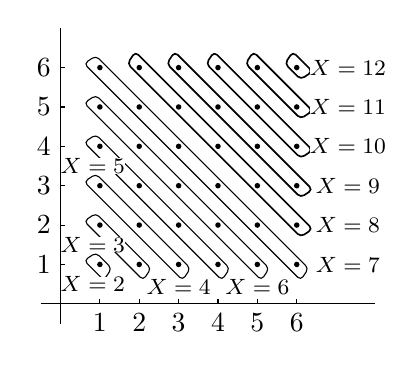
\begin{tikzpicture}[scale=0.5]
\draw(-0.5,0)--(8,0)(0,-0.5)--(0,7);
\foreach \x in{1,2,3,4,5,6}
\draw(\x,0)node[below]{$\x$}--(\x,0.12)(0,\x)node[left]{$\x$}--(0.12,\x);
\foreach \x in{1,2,3,4,5,6}\foreach \y in{1,2,3,4,5,6}
\fill(\x,\y)circle(2pt);
\foreach \x in{1.2,2.2,...,6.2}
\draw[rounded corners=1.5pt,xshift=-0.1cm,yshift=-0.1cm](\x,0.7)--(\x+0.2,1)--(1,\x+0.2)--(0.7,\x)--cycle;
\foreach \x in{1.2,2.2,...,5.2}
\draw[semithick,rounded corners=1.5pt,xshift=0.1cm,yshift=0.1cm,rotate around={180:(3.5,3.5)}]
(\x,0.7)--(\x+0.2,1)--(1,\x+0.2)--(0.7,\x)--cycle;
\foreach\x in{2,3,5}\node[fill=white,font=\footnotesize,inner sep=0pt]at(0.82,\x-1.5){$X=\x$};
\foreach \x in{4,6}\node[fill=white,font=\footnotesize,inner sep=0pt]
at(\x-1,0.42){$X=\x$};
\foreach \x in{7,...,12}\node[fill=white,font=\footnotesize,inner sep=0pt]
at(7.3,\x-6){$X=\x$};
\end{tikzpicture}
}\hfill
\subfloat[$6$点的个数$Y$的定义]{
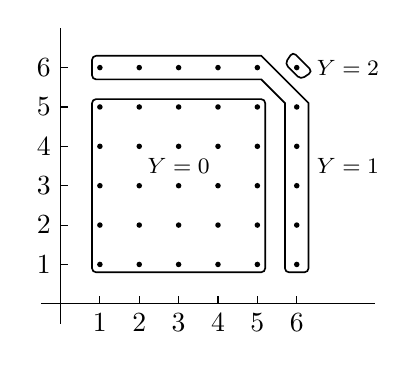
\begin{tikzpicture}[scale=0.5]
\draw(-0.5,0)--(8,0)(0,-0.5)--(0,7);
\foreach \x in{1,2,3,4,5,6}
\draw(\x,0)node[below]{$\x$}--(\x,0.2)(0,\x)node[left]{$\x$}--(0.2,\x);
\foreach \x in{1,2,3,4,5,6}\foreach \y in{1,2,3,4,5,6}
\fill(\x,\y)circle(2pt);
\draw[rounded corners=1.5pt,semithick](0.8,0.8)--(5.2,0.8)--(5.2,5.2)--(0.8,5.2)--cycle;
\draw[rounded corners=1.5pt,semithick](0.8,5.7)--(0.8,6.3)[sharp corners]--(5.1,6.3)--
(6.3,5.1)[rounded corners=1.5pt]--(6.3,0.8)--(5.7,0.8)[sharp corners]--(5.7,5.1)
--(5.1,5.7)[rounded corners=1.5pt]--cycle;
\draw[semithick,rounded corners=1.5pt,xshift=0.1cm,yshift=0.1cm,rotate around={180:(3.5,3.5)}]
(1.2,0.7)--(1.4,1)--(1,1.4)--(0.7,1.2)--cycle;
\node[fill=white,font=\footnotesize,inner sep=0pt]at(3,3.5){$Y=0$};
\node[fill=white,font=\footnotesize,inner sep=0pt]at(7.3,3.5){$Y=1$};
\node[fill=white,font=\footnotesize,inner sep=0pt]at(7.3,6){$Y=2$};
\end{tikzpicture}
}\hfill
\subfloat[最大点数$Z$的定义]{
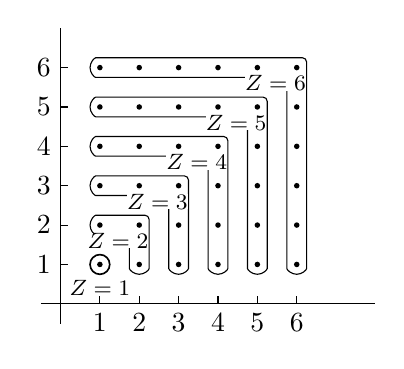
\begin{tikzpicture}[scale=0.5]
\draw(-0.5,0)--(8,0)(0,-0.5)--(0,7);
\foreach \x in{1,2,3,4,5,6}
\draw(\x,0)node[below]{$\x$}--(\x,0.2)(0,\x)node[left]{$\x$}--(0.2,\x);
\foreach \x in{1,2,3,4,5,6}\foreach \y in{1,2,3,4,5,6}
\fill(\x,\y)circle(2pt);
\draw[semithick](1,1)circle(0.25cm);
\foreach \x in {2,3,4,5,6}
\draw[rounded corners=1.5pt](1,\x-0.25)arc(270:90:0.25)--(\x+0.25,\x+0.25)
--(\x+0.25,1)arc(0:-180:0.25)--(\x-0.25,\x-0.25)--cycle;
\node[fill=white,font=\footnotesize,inner sep=0pt]at(1,0.4){$Z=1$};
\foreach \x in {2,3,4,5,6}
\node[fill=white,font=\footnotesize,inner sep=0pt]at(\x-0.54,\x-0.4){$Z=\x$};
\end{tikzpicture}
}
  \caption{同一样本空间上不同随机变量}\label{fig:2-1-2}
\end{figure}

这三个随机变量的分布列可用古典方法算得如下:
·.
% Table generated by Excel2LaTeX from sheet '1'
\begin{table}[htbp]
	\centering
	\begin{tabular}{c|cccccrrrrrr}
		X     & 2     & 3     & 4     & 5     & 6     & \multicolumn{1}{c}{7} & \multicolumn{1}{c}{8} & \multicolumn{1}{c}{9} & \multicolumn{1}{c}{10} & \multicolumn{1}{c}{11} & \multicolumn{1}{c}{12} \\\hline
		P     &   $ \frac{1}{36} $    &   $ \frac{2}{36} $    &   $ \frac{3}{36} $    &   $ \frac{4}{36} $    &    $ \frac{5}{36} $   &   $ \frac{6}{36} $    &   $ \frac{5}{36} $    &    $ \frac{4}{36} $   &    $ \frac{3}{36} $   &    $ \frac{2}{36} $   &  $ \frac{1}{36} $\\
	\end{tabular}%
	
	\begin{tabular}{c|ccc}
		$ Y $     & 0     & 1     & 2 \\\hline
		$ P $     &  $ \frac{25}{36} $     &    $ \frac{10}{36} $   & $ \frac{1}{36} $ \\
	\end{tabular}%
	
	\begin{tabular}{c|rccccc}
		$ Z $     & 1 & 2     & 3     & 4     & 5     & 6 \\\hline
		$ P $     &   $ \frac{1}{36} $    &   $ \frac{3}{36} $    &   $ \frac{5}{36} $    &   $ \frac{7}{36} $    &   $ \frac{9}{36} $    &  $ \frac{11}{36} $\\
	\end{tabular}%
\end{table}%


类似地,还可以在这个样本空间上定义其他的离散随机变量.

分布列的基本性质


(1)非负性:$: p\left(x_{t}\right) \geqslant 0, i=1,2, \cdots$;
(2)正则性:$\sum_{i=1}^{\infty} p\left(x_{i}\right)=1$.

以上两条基本性质是分布列必须具有的性质,也是判别某个数列是否成为分布列的充要条件
由离散随机变量X的分布列很容易写出X的分布函数:

\[
F(x)=\sum_{x_{1} \leqslant x} p\left(x_{i}\right)
\]

它的图形是有限级(成无穷级)的阶梯函数,具体见下面的例子.不过在离散场合,常用来描述其分布的是分布列,很少用到分布函数.因为求离散随机变量X的有关事件的概率时,用分布列比用分布函数来得更方便.

\begin{example}
	设离散随机变量 $X$ 的分布列为
	\[
	\begin{array}{c|ccc}
	x & -1 & 2 & 3 \\\hline
	P & 0.25 & 0.5 & 0.25 \\
	\end{array}
	\]
	
	试求$P(X \leqslant 0.5), P(1.5<X \leqslant 2.5)$,并写出$ X $的分布函数.
\end{example}
\begin{solution}
	
	\[
	\begin{array}{l}{P(X \leqslant 0.5)=P(X=-1)=0.25} \\ {P(1.5<X \leqslant 2.5)=P(X=2)=0.5}\end{array}
	\]
	
	\[
	  F(x) = \begin{cases}
	    0, & x<-1; \\
	    0.25, & -1 \leqslant x<2; \\
	    0.25 + 0.5 = 0.75, & 2 \leqslant x < 3; \\
	    0.25 + 0.5 + 0.25 = 1, & x \geqslant 3.
	\end{cases}
    \]
	
	$ F(x) $的图形如图~\ref{fig:2-1-3} 所示,它是一条阶梯形的曲线,在$ X $的可能取值$-1,2,3$处有跳跃点,其跳跃度分别为$ 0.25,0.5,0.25 $ .
	
	
	特别, 常量$ c $可看作仅取一个值的随机变量$X$, 即
	
	\begin{figure}
\centering
\begin{tikzpicture}[>=Stealth]
\draw[->](-2,0)--(0,0)node[below left]{$O$}--(3.5,0)node[below=1pt]{$x$};
\draw[->](0,-0.5)--(0,2.5)node[left]{$F(x)$};
\draw[thick](-2,0)--(-1,0)(-1,0.5)--(2,0.5)(2,1.5)--(3,1.5)(3,2)--(3.5,2);
\fill(-1,0.5)circle(1pt);\fill(2,1.5)circle(1pt);\fill(3,2)circle(1pt);
\filldraw[fill=white](-1,0)node[below]{$-1$}circle(1pt);\filldraw[fill=white](2,0.5)circle(1pt);
\filldraw[fill=white](3,1.5)circle(1pt);
\foreach \x in{1,2,3}\draw(\x,0.07)--(\x,0)node[below]{$\x$};
\foreach \x in{1,1.5,2}\draw(0.07,\x)--(0,\x);
\node[left]at(0,2){$1$};
\end{tikzpicture}
\caption{离散随机变量的分布函数}\label{fig:2-1-3}
\end{figure}
	
	\[
	P(X=c)=1
	\]
	
	这个分布常称为单点分布或退化分布,它的分布函数是
	
	\begin{equation}
	  F(x)= \begin{cases}
	   0, &  x < c; \\
	   1, &  x \geqslant c.
	\end{cases}  \label{eq:2.1.3}
	\end{equation}
	
	其图形为
	\begin{figure}[!ht]
  \centering
\begin{tikzpicture}[>=Stealth]
\draw[->](-0.3,0)--(0,0)node[below left]{$O$}--(4,0)node[below]{$x$};
\draw[->](0,-0.3)--(0,3)node[left]{$F(x)$};
\draw[thick](-0.3,0)--(0.8,0)node[below]{$c$}
(0.8,2)--(3.5,2);
\draw[dashed,semithick](0.8,0)--(0.8,2)--(0,2)node[left]{$1$};
\filldraw[fill=white](0.8,0)circle(1pt);
\fill(0.8,2)circle(1pt);
\end{tikzpicture}
  \caption{单点分布函数}\label{fig:2.1.4}
\end{figure}

\end{solution}

以下例子说明:在具体求离散随机变量$ X $的分布列时,关键是求出$ X $的所有可能取值及取这些值的概率.

\begin{example}
	一汽车沿一街道行驶,需要经过3个设有红绿信号灯的路口,若设每个信号灯显示红绿两种信号的时间相等,且各个估号灯工作相互独立.以$X$表示该汽车首次遇到红灯前已通过的路口数.试求$ X $的概率分布列.
\end{example}

\begin{solution}	
	由题设可知,$ X $的可能取值为$ 0,1.2.3 $又记$ A= $“汽车在第i个路口遇到红灯”,$ i=1,2,3 $.因为$ A_1,A_2,A_3 $相互独立,且
	
	\[
	P\left(A_{t}\right)=P\left(A_{t}\right)=\frac{1}{2}, \quad i=1.2 .3
	\]
	所以得
	
	\[
	\begin{array}{l}
	{P(X=0)=P\left(A_{1}\right)=\frac{1}{2}} \\
	{P(X=1)=P\left(\overline{A}_{1} A_{2}\right)=P\left(\overline{A}_{1}\right) P\left(\Lambda_{2}\right)=\frac{1}{4}} \\
	{P(X=2)=P\left(\overline{A}_{1} \overline{A}_{2} A_{3}\right)=P\left(A_{1}\right) P\left(\dot{A}_{2}\right) P\left(A_{J}\right)=\frac{1}{8}}\\
	{P(X=3)=P\left(\overline{A}_{1} \overline{A}_{2} \overline{A}_{3}\right)=P\left(\overline{A}_{1}\right) P\left(\overline{A}_{2}\right) P\left(\overline{A}_{2}\right)=\frac{1}{8}}
	\end{array}
	\]
	
	故$ X $的分布列如下:
	
	% Table generated by Excel2LaTeX from sheet '1'
	\begin{table}[htbp]
		\centering
		\begin{tabular}{c|cccc}
			$ X $     & 0     & 1     & 2     & 3 \\\hline
			$ P $     & 1/2   & 1/4   & 1/8   & 1/8 \\
		\end{tabular}%
	\end{table}%
	
\end{solution}

\subsection{连续随机变量的概率密度函数}

连续随机变量的一切可能取值是充满某个区间$ (a,b) $,在这个区间内有无穷不可列个实数,因此描述连续随机变量的概率分布不能再用分布列形式表示,而要改用概率密度函数表示.下面用一个实例来导出概率密度函数的由来.

\begin{example}
	新生婴儿的体重X是一个随机变量.假如记录很多个(例如:十万个)新生婴儿的体重,我们将各种体重的频率用直方图形式表示出来,$x$轴表示体重(单位:$ 500g $),$ y $轴表示单位长度上的频率,则以下图~\ref{fig:2-1-5} 的(a)至(c)
	表明:当$\Delta x=1$越来越小,其频率直方图形越来越光滑.
	
	\begin{enumerate}
		\item 当$\Delta x=1$ ,体重的频率直方图见图~\ref{fig:2-1-5}(a).注意,图中矩形宽度为1,高度为频率,所以所有矩形面积之和为1.此时体重$ X $的取值为$1,2, \cdots $,即$ X $是一个离散随机变量.
		\item 当 $\Delta x=0.1$ ,体重的频率直方图见图~\ref{fig:2-1-5}(b).注意,图中矩形宽度为
		$ 0.1 $,高度为:频率$ /0.1 $,所有小矩形面积之和仍为1.
		\item 当 $\Delta x \rightarrow 0$ 则体重的频率图趋于图~\ref{fig:2-1-5}(c)所示的一条光滑的曲线,其高度为概率密度值.如果记这条曲线为$ p(x) $,则$ p(x) $与$ x $轴所夹面积仍为1.此时体重$ X $的取值充满了某一区间,即X是一个连续随机变量.图中$ p(x) $就是连续随机变量X的概率密度函数.
	\end{enumerate}
	
\end{example}

\begin{figure}[!ht]
  \centering
\subfloat[$\Delta x=1$]{
\begin{tikzpicture}[>=Stealth,yscale=0.8,xscale=0.7]
\draw[decorate,decoration={snake,segment length=1mm,amplitude=0.5mm}]
(0,0)node[below]{$O$}--(0.6,0);
\draw[->](0.6,0)--(6.8,0)node[below]{$x$};
\draw[->](0,0)--(0,3)node[right]{$P/\Delta x$};
\draw[semithick](0.6,0)--(0.6,0.3)--(1.4,0.3)(1.4,0)--(1.4,0.7)--(2.2,0.7)
(2.2,0)--(2.2,1.7)(2.2,0)--(2.2,2.4)--(3,2.4)--(3,0)(3,1.7)--(3.8,1.7)--(3.8,0)
(3.8,0.8)--(4.6,0.8)--(4.6,0)(4.6,0.5)--(5.4,0.5)--(5.4,0)
(5.4,0.4)--(6.2,0.4)--(6.2,0);
\draw(1,0)--(1,-0.08)node[below]{$4$};\draw(1.8,0)--(1.8,-0.08)node[below]{$5$};
\draw(2.6,0)--(2.6,-0.08)node[below]{$6$};\draw(3.4,0)--(3.4,-0.08)node[below]{$7$};
\draw(4.2,0)--(4.2,-0.08)node[below]{$8$};\draw(5,0)--(5,-0.08)node[below]{$9$};
\draw(5.8,0)--(5.8,-0.08)node[below]{$10$};
\end{tikzpicture}
}\hfill
\subfloat[$\Delta x=0.1$]{
\begin{tikzpicture}[>=Stealth,yscale=0.8,xscale=0.6]
\draw[decorate,decoration={snake,segment length=1mm,amplitude=0.5mm}]
(0,0)node[below]{$O$}--(1,0);
\draw[->](1,0)--(6,0)node[below]{$x$};
\draw[->](0,0)--(0,3)node[right]{$P/\Delta x$};
\foreach \x in{5,6,7,8,9}\draw(\x-4,0)node[below]{$\x$}--(\x-4,-0.08);
\draw[semithick,domain=0.3:5.7,samples=100]plot(\x,{2*e^(-(\x-3)^2/2)+0.2});
\foreach \x in{1,1.1,...,5}
\draw(\x,0)--(\x,{2*e^(-(\x-3)^2/2)+0.2})--(\x+0.1,{2*e^(-(\x-3)^2/2)+0.2})
--(\x+0.1,0);
\end{tikzpicture}
}\hfill
\subfloat[$\Delta x\to 0$]{
\begin{tikzpicture}[>=Stealth,yscale=0.8,xscale=0.6]
\draw[decorate,decoration={snake,segment length=1mm,amplitude=0.5mm}]
(0,0)node[below]{$O$}--(1,0);
\draw[->](1,0)--(6,0)node[below]{$x$};
\draw[->](0,0)--(0,3)node[right]{$p(x)$};
\foreach \x in{5,6,7,8,9}\draw(\x-4,0)node[below]{$\x$}--(\x-4,-0.08);
\draw[semithick,domain=0.3:5.7,samples=100]plot(\x,{2*e^(-(\x-3)^2/2)+0.2});
\draw[dashed,semithick](2,0)--(2,1.37)(4,1.32)--(4,0);
\end{tikzpicture}
}
  \caption{新生婴儿体重$X$的频率分布}\label{fig:2-1-5}
\end{figure}

下面给出连续随机变量的概率密度函数的定义.

\begin{definition}{}{}
	设随机变量$ X $的分布函数为$ F(x) $,如果存在实数轴上的一个非负可积函数$ p(x) $,使得对任意实数$ x $有
	\begin{equation}
	  F(x)=\int_{-\infty}^{x} p(t) \dd  t, \label{eq:2.1.4}
	\end{equation}
	
	从~\ref{eq:2.1.4}式可以看出,在$ F(x) $导数存在的点上有
	\begin{equation}
	  F^{\prime}(x) = p(x), \label{eq:2.1.5}
	\end{equation}
	
	$ F(x) $是(累积)概率函数,其导数$ F'(x) $是概率密度函数,由此可看出$ p(x) $被称为概率密度函数的理由.
	
	由~\eqref{eq:2.1.5} 式,可从分布函数求得密度函数.譬如例2.1.2给出的柯西分布函数处处可导,故柯西分布的密度函数为
	
	\[
	p(x)=\frac{1}{\pi} \frac{1}{1+x^{2}},-\infty < x < +\infty.
	\]
\end{definition}

\textbf{密度函数的基本性质 }

(1)非负性:$p(x) \geqslant 0$;

(2)正则性:$: \int_{-\infty}^{+\infty} p(x) \dd  x=1$.

以上两条基本性质是密度函数必须具有的性质,也是确定或判别某个函数是否成为密度函数的充要条件.譬如已知某个函数$ p(x) $为密度函数,若$ p(x) $中有待定常数,则该常数必定是利用正则性$\int_{-\infty}^{+\infty} p(x) \dd  x=1$来确定的,见下面例子.

\begin{example}
	已知随机变量X的密度函数为
	\[
	  p(x) = \begin{cases}
	    c, & -1 \leqslant x \leqslant 1; \\
	    0, & \text{其他}.
	\end{cases}
	\]
	试求常数$ c $.
\end{example}
	
\begin{solution}
  由密度函数的正则性知
	\[
	  1=\int_{-\infty}^{+\infty} p(x) \dd  x=\int_{-1}^{1} c \dd  x=2 c.
	\]
所以由$ 2c=1 $得$ c=0.5 $.利用分段积分,我们还可求出$ X $的分布函数.
	
	当$ x<-1 $时,
	\[
	F(x)=\int_{-\infty}^{x} 0 \dd  t=0.
	\]
	
	当$-1 \leqslant x<1$时,
	\[
	F(x)=\int_{-3}^{x} 0.5 \dd  t=(x+1) / 2.
	\]
	
	当 $x \geqslant 1$ 时,
	\[
	F(x)=\int_{1}^{1} 0.5 \dd  t+\int_{1}^{x} 0 \dd  t=1.
	\]
	
	所以得$ X $的分布函数为
	\[
	  F(x) = \begin{cases}
	    0, & x<-1 ;\\
	    \frac{x+1}{2}, & -1 \leqslant x<1 ; \\
	    1, & x \geqslant 1.
	  \end{cases}
	\]
\end{solution}


由密度函数求分布函数的关键是;分布函数是一种“累积”概率,所以在计算积分时要注意积分限的合理运用.此例密度函数和分布函数的图形如图 \ref{fig:2-1-6} (a)与(b)所示, 这个分布称为区间$(-1,1)$上的均匀分布, 记为$U(-1,1)$.

\begin{figure}[!ht]
  \centering
\subfloat[$p(x)$的图形]{
\begin{tikzpicture}[>=Stealth,xscale=2,yscale=4]
\draw[->](-1.3,0)--(0,0)node[below left]{$O$}--(1.3,0)node[below]{$x$};
\draw[->](0,-0.1)--(0,0.7)node[right]{$p(x)$};
\draw[thick](-1,0.4)--(0,0.4)node[above right]{$0.5$}--(1,0.4);
\draw[dashed,semithick](-1,0.4)--(-1,0)node[below]{$-1$}(1,.4)--(1,0)node[below]{$1$};
\end{tikzpicture}
}\hspace{2cm}
\subfloat[$F(x)$的图形]{
\begin{tikzpicture}[>=Stealth,xscale=1.8,yscale=2]
\draw[->](-1.4,0)--(0,0)node[below left]{$O$}--(1.4,0)node[below]{$x$};
\draw[->](0,-0.2)--(0,1.4)node[right]{$F(x)$};
\draw[thick](-1,0)node[below]{$-1$}--(1,1)--(1.3,1);
\draw[dashed,semithick](0,1)node[left]{$1$}--(1,1)--(1,0)node[below]{$1$};
\end{tikzpicture}
}
\caption{均匀分布$U(-1,1)$的密度函数和分布函数的图形}\label{fig:2-1-6}
\end{figure}

\begin{example}
	设随机变量$X$的密度函数为
	
	\[
	  p(x) = \begin{cases}
        x, & 0 \leqslant x<1; \\
        2 - x, & 1 \leqslant x<2; \\
        0, & \text{其他}.
      \end{cases}
	\]
	
	试求$ X $的分布函数$ F(x) $.
	\end{example}
	\begin{solution}
     当$ x<0 $时,
	\[
	F(x)=\int_{-\infty}^{x} p(x) \dd  x=0
	\]
	
	当 $0 \leqslant x<1$ 时,
	\[
	F(x)=\int_{0}^{x} x \dd  x=\frac{x^{2}}{2}
	\]
	
	当 $1 \leqslant x<2$时,
	\[
	F(x)=\int_{-\infty}^{x} p(x) \dd  x=\int_{0}^{1} x \dd  x+\int_{1}^{x}(2-x) \dd  x=-\frac{x^{2}}{2}+2 x-1
	\]
	
	当 $\mathrm{I} \leqslant x<2$ 时,
	\[
	F(x)=\int_{-\infty}^{x} p(x) \dd  x=\int_{0}^{1} x \dd  x+\int_{1}^{2}(2-x) \dd  x=1
	\]
	
	综上所述,得$ X $的分布函数为
	
	\[
	F(x)=\left\{\begin{array}{ll}
	{0,} & {x<0} \\
	{\frac{x^{2}}{2},} & {0 \leqslant x<1} \\
	{-\frac{x^{2}}{2}+2 x-1,} & {1 \leqslant x<2} \\
	{1,} & {x \geqslant 2}
	\end{array}\right.
	\]
   \end{solution}


这个分布被称为辛普森分布或三角分布,其密度函数$ p(x) $和分布函数$ F(x) $的图形见下图~\ref{fig:2-1-7}.从图形上可看出:在区间$ (0,1) $上$ F(x) $是下凸函数,在区间$ (1,2) $上$ F(x) $是上凸函数.

\begin{figure}[!ht]
  \centering
\subfloat[$p(x)$的图形]{
\begin{tikzpicture}[>=Stealth,scale=2]
\draw[->](-0.2,0)--(0,0)node[below left]{$O$}--(2.4,0)node[below]{$x$};
\draw[->](0,-0.2)--(0,1.4)node[right]{$p(x)$};
\draw[thick](0,0)--(1,1)--(2,0)node[below]{$2$};
\draw[dashed,semithick](0,1)node[left]{$1$}--(1,1)--(1,0)node[below]{$1$};
\end{tikzpicture}
}\hspace{2cm}
\subfloat[$F(x)$的图形]{
\begin{tikzpicture}[>=Stealth,xscale=1.8,yscale=2,samples=100]
\draw[->](-0.2,0)--(0,0)node[below left]{$O$}--(2.4,0)node[below]{$x$};
\draw[->](0,-0.2)--(0,1.4)node[right]{$F(x)$};
\draw[thick,domain=0:1]plot(\x,{(\x)^2/2});
\draw[thick,domain=1:2]plot(\x,{-(\x)^2/2+2*\x-1});
\draw[thick](2,1)--(2.4,1);
\draw[dashed,semithick](0,1)node[left]{$1$}--(2,1)--(2,0)node[below]{$2$};
\draw(1,0.05)--(1,0)node[below]{$1$};
\end{tikzpicture}
}
  \caption{辛普森分布}\label{fig:2-1-7}
\end{figure}

以下我们对密度函数与分布列的异同点作一些说明.

在离散随机变量场合,

\[
P(a<X \leqslant b)=\sum_{a<x_{i} \leqslant b} p\left(x_{i}\right)
\]

其中诸$ x_i $;为$ X $的可能取值.

而在连续随机变量场合,

\[
P(a<X \leqslant b)=\int_{a}^{b} p(x) \dd  x
\]

其含义见下图.



\begin{figure}[!ht]
  \centering
\begin{tikzpicture}[>=Stealth,xscale=2.2,yscale=2,samples=100]
\draw[->](-0.2,0)--(0,0)node[below left]{$O$}--(2.4,0)node[below]{$x$};
\draw[->](0,-0.2)--(0,1.4)node[right]{$p(x)$};
\draw[thick,domain=-0.2:2.3]plot(\x,{e^(-3*(\x-1.05)^2)});
\filldraw[thick,fill=gray!30,domain=0.5:1.6](0.5,0)node[below]{$a$}--(0.5,{e^(-3*(0.5-1.05)^2)})--
plot(\x,{e^(-3*(\x-1.05)^2)})--(1.6,{e^(-3*(1.6-1.05)^2)})--(1.6,0)node[below]{$b$}--cycle;
\node at(1.05,0.2){$P(a<X\leq b)$};
\end{tikzpicture}
  \caption{连续随机变量场合的概率}\label{fig:2.1.8}
\end{figure}

从这个意义上讲,概率密度函数与概率分布列所起的作用是类似的,但它们之间的差别也是明显的,具体有

\begin{enumerate}
	\item 离散随机变量的分布函数F(x)总是右连续的阶梯函数,而连续随机变量的分布函数$ F(x) $一定是整个数轴上的连续函数,因为对任意点$ x $的增量$\Delta x$,相应分布函数的增量总有
	\[
	F(x+\Delta x)-F(x)=\int_{x}^{x+\Delta x} p(x) \dd  x \longrightarrow 0, \quad(\Delta x \rightarrow 0)
	\]
	\item 离散随机变量$ X $在其可能取值的点$x_{1}, x_{2}, \cdots, x_{n}, \cdots$上的概率不为$ 0 $,而连续随机变量$ X $在$(-\infty,+\infty)$上任一点$ a $的概率恒为$ 0 $,即
	\[
	P(X=a)=\int_{a}^{a} p(x) \dd  x=0
	\]
	这表明:不可能事件的概率为$ 0 $,但概率为0的事件不一定是不可能事件;类似地,必然事件的概率为$ 1 $,但概率为$ 1 $的事件不一定是必然事件.
	\item 由于连续随机变量$ X $仅取一点的概率恒为$ 0 $,从而在事件“$a \leqslant X \leqslant b$”
	中减去$ x=a $或减去$ X=b $,不影响其概率,即
	\[
	P(a \leqslant x \leqslant b)=P(a<X \leqslant b)=P(a \leqslant X<b)=P(a<X<b)
	\]
	这给计算带来很大方便.而这个性质在离散随机变量场合是不存在的,在离散随机变量场合计算概率要“点点计较”.
	\item 由于在若干点上改变密度函数$ p(x) $的值并不影响其积分的值,从而不影响其分布函数$ F(x) $的值,这意味着一个连续分布的密度函数不唯一.譬如在例2.1.7中,改变$ x=-1 $和x=1处$ p(x) $的值如下:
	\[
	p_{1}(x)=\left\{\begin{array}{ll}{0.5,} & {-1 \leqslant x \leqslant 1} \\ {0,} & {\text{其他} \text { th }}\end{array}\right. p_{2}(x)=\left\{\begin{array}{ll}{0.5,} & {-1<x<1} \\ {0} & { \neq 4}\end{array}\right.
	\]
	它们都是$ (-1,1) $上均匀分布的密度函数.但仔细考察这两个函数$ p_1(x) $和$ p_2(x) $,可以发现
	\[
	P\left(p_{1}(x) \neq p_{2}(x)\right)=P(X=-1)+P(X=1)=0
	\]
	可见这两个函数在概率意义上是无差别的,在此称$ p_1(x) $与$ p_2(x) $是“几乎处处相等”,其含义是:它们不相等处的点组成集合的概率为$ 0 $.这就是概率论与微积分不同之处,也是概率论的魅力之处.
	除了离散分布和连续分布之外,还有既非离散又非连续的分布,见下例.
\end{enumerate}

\begin{example}
	以下的函数$ F(x) $确是一个分布,它的图形如图~\ref{fig:2-1-9}所示.
	\[
	F(x)=\left\{\begin{array}{ll}{0,} & {x<0} \\ {\frac{1+x}{2},} & {0 \leqslant x<1} \\ {1,} & {x \geqslant 1}\end{array}\right.
	\]
	
	从图上可以看出:它既不是阶梯函数,又不是连续图~\ref{fig:2-1-9}既非离散、又非函数,所以它既非离散的又非连续的分布.它是新的一连续的分布函数示例类分布,本书将不研究此类分布,只让大家知道山外有山,需要不断学习与研究.
\end{example}

下面我们再给出一些连续随机变量的例子.

\begin{figure}[!ht]
  \centering
\begin{tikzpicture}[>=Stealth,scale=2]
\draw[->](-0.3,0)--(0,0)node[below left]{$O$}--(1.6,0)node[below]{$x$};
\draw[->](0,-0.2)--(0,1.4)node[right]{$F(x)$};
\draw[thick](0,0.5)node[left]{$0.5$}--(1,1)--(1.5,1)(-0.3,0)--(0,0);
\filldraw[fill=white](0,0)circle(0.5pt);
\fill(0,0.5)circle(0.5pt);
\draw[semithick,dashed](0,1)node[left]{$1$}--(1,1)--(1,0)node[below]{$1$};
\end{tikzpicture}
  \caption{既非离散、又非连续的分布函数示例}\label{fig:2-1-9}
\end{figure}

\begin{example}
	某种型号电子元件的寿命$ X $(以小时计)具有以下的概率密度函数
	\[
	  p(x) = \begin{cases}
	   \frac{1000}{x^2}, &x>1000;\\
	   0, & \text{其他}.
	  \end{cases}
	\]
	现有一大批此种元件(设各元件工作相互独立),问
	
	\begin{enumerate}
		\item 任取1只,其寿命大于1500小时的概率是多少?
		\item 任取4只,4只寿命都大于1500小时的概率是多少?
		\item 任取4只,4只中至少有1只寿命大于1500小时的概率是多少?
		\item 若已知一只元件的寿命大于1500小时,则该元件的寿命大于2000小时的概率是多少?
	\end{enumerate}
\end{example}

\begin{solution}
\begin{enumerate}
	\item \[
	P\{X>1500\}=\int_{1500}^{+\infty} \frac{1000}{x^{2}} \dd  x=\left(-\frac{1000}{x}\right)_{1500}^{+\infty}=\frac{2}{3}
	\]
	\item 各元件工作独立,因此所求概率为
	\[
	P\{\text{四只原件寿命都大于}1500\}=[P(X>1500)]^{4}=\left(\frac{2}{3}\right)^{4}=\frac{16}{81}
	\]
	\item 所求概率为
	\[\begin{gathered}
	P\{\text{四只中至少一只寿命大于}1500\} \hfill \\
	=1-P\{4\text{只元件寿命都小于等于}1500\} \hfill \\
	=1-\left(1-\frac{2}{3}\right)^{4}=\frac{80}{81} \hfill \\
	\end{gathered} \]
	\item 这是求条件概率$P\{X>2000 | X>1500\}$ ,记
	\[
	A=\{X>1500|, B=\{X>2000\}
	\]
	因为$P(A)=2 / 3, P(B)=1 / 2$,且$B \subset A$,所以
	\[
	P(B | A)=\frac{P(A B)}{P(A)}=\frac{P(B)}{P(A)}=\frac{3}{4}
	\]
\end{enumerate}
\end{solution}

\begin{example}
	向区间$ (0,a) $上任意投点, 用$X$表示这个点的坐标.设这个点落在$ (0,a) $中任一小区间的概率与这个小区间的长度成正比,而与小区间位置无关.求$ X $的分布函数和密度函数.
\end{example}

\begin{solution}	
	记$ X $的分布函数为$ F(x) $,则
	当$ x<0 $时,因为$\{X \leqslant x\}$是不可能事件,所以$F(x)=P(X \leqslant x)=0$;
	
	当$x \geqslant a$时,因为$\{ X \leqslant x \}$是必然事件,所以$F(x)=P(X \leqslant x)=1$;
	当$0 \leqslant x<a$时,有$F(x)=P(X \leqslant x)=P(0 \leqslant X \leqslant x)=k x$,其中$ k $为比例系数.因为$ 1=F(a)=ka $,所以得$ k=1/a $.
	于是$ X $的分布函数为
	
	\[
	F(x) = \begin{cases} 0, & {x<0} \\
      \frac{x}{a}, & 0 \leqslant x<a \\
      1, & x \geqslant a
      \end{cases}
	\]
	
	
	下求$ X $的密度函数$ p(x) $.
	
	当$ x<0 $或$ x>a $时,$ p(x)=F'(x)=0 $;
	
	当$ 0<x<a $时,$ p(x)=F'(x)=1/a $;
	
	而在$ x=0 $和$ x=a $处, $ p(x) $可取任意值,一般就近取值为宜,这不会影响概率的计算,因为它们是几乎处处相等的密度函数.于是$ x $的密度函数为
	
	\[
	p(x)=\begin{cases}
	\frac{1}{a}, & 0<x<a; \\
	0, & \text{其他}.
	\end{cases}
	\]
	
	这个分布就是区间$ (0,a) $上的均匀分布,记为$ U(0,a) $,其密度函数$ p(x) $
	和分布函数$ F(x) $的图形见下图~\ref{fig:2-1-10}.
\end{solution}



\begin{figure}[!ht]
  \centering
\subfloat[$p(x)$的图形]{
\begin{tikzpicture}[>=Stealth,scale=2]
\draw[->](-0.3,0)--(0,0)node[below left]{$O$}--(2.1,0)node[below]{$x$};
\draw[->](0,-0.2)--(0,1.4)node[right]{$p(x)$};
\draw[thick](1.6,0.9)--(0,0.9)node[left]{$\frac1a$};
\draw[dashed,semithick](1.6,0.9)--(1.6,0)node[below]{$a$};
\end{tikzpicture}
}\hspace{2cm}
\subfloat[$F(x)$的图形]{
\begin{tikzpicture}[>=Stealth,scale=2,thick]
\draw[->](-0.3,0)--(0,0)node[below left]{$O$}--(2.1,0)node[below]{$x$};
\draw[->](0,-0.2)--(0,1.4)node[right]{$F(x)$};
\draw[thick,dashed](1.6,1)--(0,1)node[left]{$1$};
\draw[dashed,semithick](1.6,1)--(1.6,0)node[below]{$a$};
\draw (0,0) -- (1.6,1) -- ++ (0.3,0);
\end{tikzpicture}
}
\caption{$(0,a)$上的均匀分布}\label{fig:2-1-10}
\end{figure}

其实此例就是第一章中所说的几何概率,这也建立了几何概率与均匀分布的联系.

\begin{example}
	设连续随机变量X的密度函数为
	
	\[
	  p(x) = \begin{cases}
	    4 x^3, & 0 < x < 1 ; \\
	    0, & \text{其他}.
	  \end{cases}
	\]
	\begin{enumerate}[label=(\arabic*)]
	  \item  已知$ P(X<a)=P(X>a) $,试求常数$ a $(此$ a $称为该分布的中位数).
	  \item 已知$ P(X>b)=0.05 $,试求常数$ b $.
	\end{enumerate}
\end{example}
\begin{solution}
    \begin{inparaenum}[(1)]
	  \item  因为$ X $为连续随机变量,所以有$ P(X=a)=0 $,从而
	  \[
	    P(X < a) + P(X > a) = 1.
	  \]
	
	由$ P(X<a)=P(X>a) $,可以得$ P(X<a)=0.5 $.而
	  \[
	    P(X < a) = \int_{0}^{a} 4 x^{3} \dd x=a^{4},
	  \]
	所以从$ a^4=0.5 $解得$a=\sqrt[4]{0.5}=0.8409$.这里的$ a=0.8409 $把该分布的密度函数下的面积分为两部分,$ a $点左侧与右侧面积各为$ 0.5 $,故称a点为该分布的中位数(详见2.7.4).
	
	\item  因为
	\[
	  P (X > b) = \int_{b}^{1} 4 x^{3} \dd  x = 1 - b^{4},
	\]
	所以从$1-b^{4}=0.05$解得$b=\sqrt[4]{0.95}=0.9873$.
  \end{inparaenum}
\end{solution}


\begin{xiti}
\item 口袋中有$ 5 $只球,编号为$ 1,2,3,4,5 $.从中任取$ 3 $只,以X表示取出的$ 3 $只球中的最大号码.
\begin{enumerate}
  \item 试求$ X $的分布列;
  \item 写出$ X $的分布函数,并作图.
\end{enumerate}

\item 一颗骰子撇两次,以$ X $表示两次中所得的最小点数.
\begin{enumerate}
  \item 试求$ X $的分布列;
  \item 写出X的分布函数.
\end{enumerate}

\item 口袋中有$ 7 $个白球、$ 3 $个黑球.
  \begin{enumerate}
    \item 每次从中任取一个不放回,求首次取出白球的取球次数$ X $的概率分布列;
    \item 如果取出的是黑球则不放回,而另外放入一个白球,此时$ X $的概率分布列如何.
  \end{enumerate}

\item 有$ 3 $个盒子,第一个盒子装有1只白球、$ 4 $只黑球;第二个盒子装有$ 2 $只白球、3只黑球;第三个盒子装有$ 3 $只白球、$ 2 $只黑球.现任取一个盒子,从中任取3只球.以$ X $表示所取到的白球数.
  \begin{enumerate}
    \item 试求$ X $的概率分布列;
    \item 取到的白球数不少于2只的概率是多少?
  \end{enumerate}

\item 一批产品共有100件,其中10件是不合格品.根据验收规则,从中任取5件产品进行质量检验,假如5件中无不合格品,则这批产品被接收,否则就要重新对这批产品逐个检验.
  \begin{enumerate}
    \item 试求5件中不合格品数$ X $的分布列;
    \item 需要对这批产品进行逐个检验的概率是多少?
  \end{enumerate}

\item 设随机变量$ X $的分布函数为
\[
  F(x) = \begin{cases}
    0, & x \le 0; \\
    1 / 4, & 0 \leqslant x<1; \\
    1 / 3, & 1 \leqslant x<3; \\
    1 / 2, & 3 \leqslant x<6; \\
    1, & x \geqslant 6.
  \end{cases}
\]
试求X的概率分布列及$P(X<3), P(X \leqslant 3), P(X>1), P(X \geqslant 1)$.

\item 设随机变量$X$的分布函数为
\[
  F(x) = \begin{cases}
    0, & x<1; \\
    \ln x, & 1 \leqslant x<\ee; \\
    1, & x \geqslant \ee.
  \end{cases}
\]
试求 $P(X<2), P(0<X \leqslant 3), P(2<X<2.5)$.

\item 若$P\left\{X \geqslant x_{1}\right\}=1-\alpha, P\left\{X \leqslant x_{2}\right\}=1-\beta$,其中$ x_1<x_2 $,试求$P \{ x_{1} \leqslant X \leqslant x_{2} \}$.

\item 从$ 1,2,3,4,5 $五个数中任取三个,按大小排列记为$ x_1<x_2<x_3 $,令$ X=x_2 $,试求
  \begin{enumerate}
    \item $X$的分布函数;
    \item $P(X<2)$及$P(X>4)$.
  \end{enumerate}

\item 设随机变量$X$的密度函数为

\[
  p(x) = \begin{cases}
    1-|x|, & -1 \leqslant x \leqslant 1; \\
    0, & \text{其他}.
  \end{cases}
\]
试求$X$的分布函数.

\item 如果$X$的密度函数为
\[
  p(x) = \begin{cases}
    x, & 0 \le x < 1 ; \\
    2 - x, & 1 \le x < 2; \\
    0, & \text{其他}.
  \end{cases}
\]
试求$P(X\le1.5)$.

\item 设随机变量$X$的密度函数为
\[
  p(x) = \begin{cases}
    A\cos x, & |x| \le \frac\pi2; \\
    0, & |x| > \frac\pi2.
  \end{cases}
\]
试求
\begin{enumerate}
  \item 系数$A$;
  \item $X$落在区间$(0,\pi/4)$内的概率.
\end{enumerate}

\item 设随机变量$ X $的密度函数为
\[
  F(x) = \begin{cases}
    0, & x<0; \\
    A x^{2}, & 0 \leqslant x<1; \\
    1, & x \geqslant 1.
  \end{cases}
\]
试求
  \begin{enumerate}
    \item 系数$ A $;
    \item $ X $落在区间$ (0.3,0.7) $内的概率;
    \item $ X $的密度函数.
  \end{enumerate}

\item 学生完成一道作业的时间$ X $是一个随机变量,单位为小时.它的密度函数为
\[
  p(x) = \begin{cases}
    c x^{2}+x, & 0 \leqslant x \leqslant 0.5; \\
    0, & \text{其他}.
  \end{cases}
\]
  \begin{enumerate}
    \item 确定常数$ c $;
    \item 写出$ X $的分布函数;
    \item 试求在$ 20$min内完成一道作业的概率;
    \item 试求$ 10$min以上完成一道作业的概率.
  \end{enumerate}

\item 设随机变量$ X $和$ Y $同分布,$ X $的密度函数为
\[
  p(x) = \begin{cases}
    \frac{3}{8} x^{2}, & 0<x<2; \\
    0, & \text{其他}.
  \end{cases}
\]
已知事件$ A=\{X>a\} $和$ B=\{Y>a\} $独立, 且$P(A \cup B)=3 / 4$, 求常数$ a $.

\item 设连续随机变量X的密度函数$ p(x) $是一个偶函数,$ F(x) $为$ X $的分布函数,求证对任意实数$ a>0 $,有
  \begin{enumerate}
    \item $F(-a)=1-F(a)=0.5-\int_{0}^{a} p(x) d x_{i}$;
    \item $P( | X | <a)=2 F(a)-1$;
    \item $P(|X|>a)=2[1-F(a)]$.
  \end{enumerate}
\end{xiti}

\section{随机变量的数学期望}

我们已经知道,每个随机变量都有一个分布(分布列、密度函数或分布函数),不同的随机变量可能拥有不同的分布,也可能拥有相同的分布.分布全面地描述了随机变量取值的统计规律性,由分布可以算出有关随机变量事件的概率.除此以外由分布还可以算得相应随机变量的均值、方差、分位数等特征数.这些特征数各从一个侧面描述了分布的特征.譬如,初生婴儿的体重是一个随机变量,其平均重量就是从一个侧面描述了体重的特征.已知随机变量的分布,如何求其均值,是本节需要研究的问题.

本节将介绍随机变量最重要的特征数:数学期望.

\subsection{数学期望的概念}

“期望”在我们日常生活中常指有根据的希望,而在概率论中,数学期望源于历史上一个著名的分赌本问题.
例2.2.1(分赌本问题)17世纪中叶,一位赌徒向法国数学家帕斯卡(1623一1662)提出一个使他苦恼长久的分赌本问题:甲、乙两赌徒赌技相同,各出赌注50法郎,每局中无平局.他们约定,谁先赢三局,则得全部赌本100法郎.当甲赢了二局、乙赢了一局时,因故要中止赌博.现问这100法郎如何分才算公平?

这个问题引起了不少人的兴趣.首先大家都认识到:平均分对甲不公平;全部归甲对乙不公平;合理的分法是,按一定的比例,甲多分些,乙少分些.所以问题的焦点在于:按怎样的比例来分.以下有两种分法:

(1)甲得100法郎中的2/3,乙得100法郎中的1/3.这是基于已赌局数:甲赢了二局、乙赢了一局.

(2)1654年帕斯卡提出如下的分法:设想再赌下去,则甲最终所得X为一个随机变量,其可能取值为0或100.再赌二局必可结束,其结果不外乎以下四种情况之一:

\begin{center}
	甲甲、甲乙、乙甲、乙乙
\end{center}

其中“甲乙”表示第一局甲胜第二局乙胜.因为赌技相同,所以在这四种情况中有三种可使甲获100法郎,只有一种情况(乙乙)下甲获0法郎.所以甲获得100法郎的可能性为$ 3/4 $,获得0法郎的可能性为$ 1/4 $,即$ X $的分布列为

\[
\begin{array}{c|cc}{x} & {0} & {100} \\ \midrule
P & {0.25} & {0.75} \\
\end{array}
\]

经上述分析,帕斯卡认为,甲的“期望”所得应为:$0 \times 0.25+100 \times 0.75=75$
(法郎).即甲得75法郎,乙得25法郎.这种分法不仅考虑了已赌局数,而且还包括了对再赌下去的一种“期望”,它比(1)的分法更为合理.

这就是数学期望这个名称的由来,其实这个名称称为“均值”更形象易懂.对上例而言,也就是再赌下去的话,甲“平均”可以赢75法郎.

现在我们来逐步分析如何由分布来求“均值”.

(1)算术平均:如果有$ n $个数$x_{1}, x_{2}, \cdots, x_{n}$.,那么求这$ n $个数的算术平均是很简单的事,只需将此$ n $个数相加后除n即可.

(2)加权平均:如果这$ n $个数中有相同的,不妨设其中有$ n $;个取值为$x_{i}, i=1,2, \cdots, k$.将其列表为

\[
\begin{array}{c|cccc}
\toprule
\text{取值}    &  x_1     &    x_1     &    \cdots     &   x_k \\\midrule
\text{频数}    &  n_1     &    n_2     &     \cdots    &   n_k \\\midrule
\text{频率}    &  n_1/n   &    n_2/n   &     \cdots    &   n_k/n \\
\bottomrule
\end{array}
\]


则其“均值”应为

\[
\frac{1}{n} \sum_{i=1}^{k} n_{\dot{r}} x_{i}=\sum_{i=1}^{k} \frac{n_{i}}{n} x_{i}
\]

其实这个“加权”平均的权数“就是出现数值$ x $;的频率,而频率在$ n $很大时,就稳定在其概率附近.

(3)对于一个离散随机变量$ X $,如果其可能取值为$x_{1}, x_{2}, \cdots, x_{n}$.若将这$ n $个数相加后除$ n $作为“均值”,则肯定是不妥的.其原因在于$ X $取各个值的概率是不同的,概率大的出现的机会就大,则在计算中其权也应该大.而上例分配赌本问题启示我们:用取值的概率作为一种“权数”作加权平均是十分合理的.

经以上分析,我们就可以给出数学期望的定义.

\subsection{数学期望的定义}

\begin{definition}{}{}
	设离散随机变量$ X $的分布列为
	
	\[
	p\left(x_{i}\right)=P\left(X=x_{i}\right), i=1,2, \cdots, n, \cdots
	\]
	
	如果
	
	\[
	\sum_{i=1}^{+\infty}\left|x_{i}\right| p\left(x_{i}\right)<+\infty
	\]
	
	则称
	
	\begin{equation}
	E(X)=\sum_{i=1}^{+\infty} x_{i} p\left(x_{i}\right) \label{eq:2.2.1}
	\end{equation}
	为随机变量$ X $的\textbf{数学期望},\index{S!数字特征!数学期望} 或称为该分布的数学期望,简称期望或均值.若级数$\sum_{k=1}^{+\infty}\left|x_{k}\right| p\left(x_{k}\right)$不收敛,则称$ X $的数学期望不存在.
\end{definition}

以上定义中,要求级数绝对收敛的目的在于使数学期望唯一.因为随机变量的取值可正可负,取值次序可先可后,由无穷级数的理论知道,如果此无穷级数绝对收敛,则可保证其和不受次序变动的影响.由于有限项的和不受次序变动的影响,故其数学期望总是存在的.

连续随机变量数学期望的定义和含义完全类似于离散随机变景场合,只要将分布列$ p(x_i) $改为密度函数、将求和改为求积就可.

\begin{definition}{}{}
	设连续随机变量$ X $的密度函数为$ p(x) $.如果
	\[
	\int_{-\infty}^{+\infty}|x| p(x) \dd  x<+\infty
	\]
	则称
	
	\begin{equation}
	E(X)=\int_{-\infty}^{+\infty} x p(x) \dd  x \label{eq:2.2.2}
	\end{equation}
	为$ X $的数学期望,或称为该分布$ p(x) $的数学期望,简称期望或均值.若$\int_{-\infty}^{+\infty}|x| p(x) \dd  x$不收敛,则称$ X $的数学期望不存在.
	
\end{definition}

\begin{example}
	在一个人数为$ N $的人群中普查某种疾病,为此要抽验$ N $个人的血.如果将每个人的血分别检验,则共需检验$ N $次.为了能减少工作量,一位统计学家提出一种方法:按$ k $个人一组进行分组,把同组$ k $个人的血样混合后检验,如果这混合血样呈阴性反应,就说明此$ k $个人的血都呈阴性反应,此$ k $个人都无此疾病,因而这$ k $个人只要检验1次就够了,相当于每个人检验$ 1/k $次,检验的工作量明显减少了.如果这混合血样呈阳性反应,就说明此$ k $个人中至少有一人的血呈阳性反应,则再对此$ k $个人的血样分别进行检验,因而这$ k $个人的血要检验$ 1+k $次,相当于每个人检验$ 1+1/k $次,这时增加了检验次数.假设该疾病的发病率为$ p $,且得此疾病相互独立.试问此种方法能否减少平均检验次数?
\end{example}
	
	\begin{solution}
	
	令$ X $为该人群中每个人需要的验血次数,则$ X $的分布列为
	
	\begin{table}[htbp]
		\centering
		\begin{tabular}{c|cc}
			$ x $	&    $ 1 / k $      &  $ 1+1 / k $ \\\midrule
			$ P $	&    $ (1-p)^{k} $  &  $ 1-(1-p)^{k} $\\
		\end{tabular}%
	\end{table}%
	
\end{solution}

所以每人平均验血次数为

\[
E(X)=\frac{1}{k}(1-p)^{k}+\left(1+\frac{1}{k}\right)\left[1-(1-p)^{k}\right]=1-(1-p)^{k}+\frac{1}{k}
\]

去由此可知,只要选择$ k $使

\[
1-(1-p)^{k}+\frac{1}{k}<1, \text{或} \quad(1-p)^{k}>\frac{1}{k}
\]

,就可减少验血次数,而且还可适当选择$ k $使其达到最小.譬如,当$ p=0.1 $时对不同的$ k $,$ E(X) $的值如表~\ref{tab:2.21}所示.从表中可以看出:当$k \geqslant 34$时,平均验血次数超过1,即比分别检验增加工作量;而当$k \leqslant 33$时,平均验血次数在不同程度上得到了减少,特别在$k_{0}=4$时,平均验血次数最少,验血工作量可减少$ 40\% $.

% Table generated by Excel2LaTeX from sheet '1'
\begin{table}[htbp]
	\centering
	\caption{$ p=0.1 $时的$ E(X) $值}
	\begin{tabular}{c|ccccccccc}
		\toprule
		k     & 2     & 3     & 4     & 5     & 8     & 10    & 30    & 33    & 34 \\\midrule
		E(x)  & 0.69  & 0.604 & 0.594 & 0.61  & 0.695 & 0.751 & 0.991 & 0.994 & 1.0016 \\\bottomrule
	\end{tabular}%
	\label{tab:2.21}%
\end{table}%


我们也可以对不同的发病率$ p $计算出最佳的分组人数$ k_0 $,见下表~\ref{tab:2.2.2}.从表中也可以看出:发病率$ p $越小,则分组检验的效益越大.譬如在$ p=0.01 $时,若取11人为一组进行验血,则验血工作量可减少$ 80\% $左右.这正是美国二战期间大量征兵时,对新兵验血所采用的减少工作量的措施.

% Table generated by Excel2LaTeX from sheet '1'
\begin{table}[htbp]
	\centering
	\caption{不同发病率$ p $时的最佳分组人数$ k_0 $及其$ E(x) $}
	\begin{tabular}{c|ccccccc}
		\toprule
		$ p $     & 0.14  & 0.1   & 0.08  & 0.06  & 0.04  & 0.02  & 0.01 \\\midrule
		$ k_0 $    & 3     & 4     & 4     & 5     & 6     & 8     & 11 \\\midrule
		$ E(x) $  & 0.697 & 0.594 & 0.534 & 0.466 & 0.384 & 0.274 & 0.205 \\\bottomrule
	\end{tabular}%
	\label{tab:2.2.2}%
\end{table}%

\begin{example}
	每张福利彩票售价5元,各有一个对奖号.每售出100万张设一个开奖组,用摇奖器当众摇出一个6位数的中奖号码(可以认为从000000到999999的每个数都等可能出现),对奖规则如下:
	\begin{enumerate}
		\item 对奖号与中奖号码的最后一位相同者获六等奖,奖金10元.
		\item 对奖号与中奖号码的最后二位相同者获五等奖,奖金50元.
		\item 对奖号与中奖号码的最后三位相同者获四等奖,奖金500元.
		\item 对奖号与中奖号码的最后四位相同者获三等奖,奖金5000元.
		\item 对奖号与中奖号码的最后五位相同者获二等奖,奖金50000元.
		\item 对奖号与中奖号码的全部相同者获一等奖,奖金500000元.另外规定,只领取其中最高额的奖金.试求每张彩票的平均所得奖金额.
	\end{enumerate}
\end{example}
	
	\begin{solution} 以$ X $记一张彩票的奖金额,则$ X $的分布列如下:
	\[
	\begin{array}{c|ccccccc}
	\toprule
	X     & 500000 & 50000 & 5000  & 500   & 50    & 10    & 0 \\\midrule
	P     & 0.000001 & 0.00009 & 0.00009 & 0.0009 & 0.009 & 0.09  & 0.9 \\\bottomrule
	\end{array}
	\]
	
	
	所以每张彩票的平均所得为
	
	\[
	E(X)=0.5+0.45+0.45+0.45+0.45+0.9+0=3.2
	\]
	
	这也意味:每一开奖组把筹得的500万元中的320万元以奖金形式返回给彩民,其余180万元则可用于福利事业及管理费用.
	
	从这个例子也可以看出,彩票中奖与否是随机的,但一种彩票的平均所得是可以预先算出的,计算平均所得也是设计一种彩票的基础.
	
\end{solution}

\begin{example}
	设$X$服从区间$ (a,b) $上的均匀分布,求$ E(x) $.
\end{example}
	
	\begin{solution}
    由例2.1.11知$ X $的密度函数为
	
	\[
	  p(x) = \begin{cases}
	    \frac{1}{b-a}, & a<x<b;  \\
        0, &  \text{其他}.
	  \end{cases}
	\]
	
	所以
	
	\[
	E(X)=\int_{a}^{b} x \cdot \frac{1}{b-a} d x=\frac{1}{b-a} \cdot\left.\frac{x^{2}}{2}\right|_{a} ^{b}=\frac{a+b}{2}
	\]
	
	这个结果是可以理解的,因为X在区间$ (a,b) $上的取值是均匀的,所以它的平均取值当然应该是$ (a,b) $的“中点”,即$ (a+b)/2 $.
	
	
\end{solution}

\begin{example}
	柯西分布的数学期望不存在.因为柯西分布的密度函数为
	
	\[
	p(x)=\frac{1}{\pi} \frac{1}{1+x^{2}},-\infty<x<+\infty,
	\]
	
	所以由
	
	\[
	\int_{-\infty}^{+\infty}|x| \cdot \frac{1}{\pi} \frac{1}{1+x^{2}} \dd  x=+\infty.
	\]
	
	知$ E(X) $不存在.
	
\end{example}

\subsection{数学期望的性质}

按照随机变量X的数学期望$ E(X) $的定义,$ E(X) $由其分布唯一确定.如今
若要求随机变量x的一个函数$ g(X) $的数学期望,当然要先求出$ Y=g(X) $的分布,再用此分布来求$ E(Y )$.这一过程可用下面例子说明.

\begin{example}
	已知随机变量$ X $的分布列如下
	
	\[
	\begin{array}{c|ccccc}
	X &{-2} & {-1} & {0} & {1} & {2} \\ \midrule
	P & {0.2} & {0.1} & {0.1} & {0.3} & {0.3}
	\end{array}
	\]
	
	要求$ Y=X^2 $的数学期望,为此要分两步进行:
	
	第一步,先求$ Y=X^2 $的分布,这可从$ X $的分布导出,即
	
	\[
	\begin{array}{c|ccccc}
	X^2    & (-2)^2 & (-1)^2 & 0^2    & 1^2    & 2^2 \\\midrule
	P     & 0.2   & 0.1   & 0.1   & 0.3   & 0.3 \\
	\end{array}
	\]
	
	然后对相等的值进行合并,并把对应的概率相加,可得
	
	\[
	\begin{array}{c|ccc}
	X^2    & 0     & 1     & 4 \\\midrule
	P     & 0.1   & 0.4   & 0.5 \\
	\end{array}
	\]
	
	第二步,利用$ X^2 $的分布求$ E(X^2) $,即得
	
	\[
	  E(X^{2})=0 \times 0.1+1 \times 0.4+4 \times 0.5=2.4.
	\]
	
	假如我们用等值合并前的分布求$ E(X^2) $,可得相同的结果
	
	\[
	  E(X^{2})=(-2)^{2} \times 0.2+(-1)^{2} \times 0.1+0^{2} \times 0.1+1^{2} \times 0.3+2^{2} \times 0.3=2.4
	\]
	
	这两种算法本质上是一回事,但后者的计算实质上是在$ X $的分布$ (0.2,
	0.1,0.1,0.3,0.3) $基础上、而将取值改为$\left((-2)^{2},(-1)^{2}, 0^{2}, 1^{2}, 2^{2}\right)$计算出来的.由此启发我们:若进一步要求$ E(X^3) $和$ E(X^4) $,我们不需要先求$ X^3 $的分布和$ E\left(X^{4}\right) $的分布,而直接用$ X $的分布来求,具体如下.
	
	\[
	\begin{aligned}
	 E (X^{3} ) &=(-2)^{3} \times 0.2+(-1)^{3} \times 0.1+0^{3} \times 0.1+1^{3} \times 0.3+2^{3} \times 0.3=0, \\
    E(X^{4}) &=(-2)^{4} \times 0.2+(-1)^{4} \times 0.1+0^{4} \times 0.1+1^{4} \times 0.3+2^{4} \times 0.3=8.4.
	\end{aligned}
	\]
	
\end{example}



一般场合,有如下定理:
\begin{theorem}{}{}
	若随机变量$ X $的分布用分布列$ p(x_i) $或用密度函数$ p(x) $表示,则$ X $的某一函数$ g(X) $的数学期望为
	
	\begin{equation}\label{eq:2.2.3}
	E[g(X)] = \begin{cases}
	  \sum_{i} g\left(x_{i}\right) p\left(x_{i}\right), & \text{在离散场合;} \\
      \int_{-\infty}^{+\infty} g(x) p(x) \dd  x, & \text{在连续场合.}
	\end{cases}
	\end{equation}
	
	这里所涉及的数学期望都假设存在.
	
	这个定理的证明涉及更多的工具,在此省略了.现基于这个定理来证明数学期望的几个常用性质,以下均假定所涉及的数学期望是存在的.
	
\end{theorem}

\begin{property}
	
	若$ c $是常数,则$ E(c)=c $.
	
\end{property}

\begin{proof}
	如果将常数$ c $看作仅取一个值的随机变量$ X $,则有$ P(X=c)=1 $,从而其数学期望 $ E(c)=E(X)=c \times 1=c $.
\end{proof}

\begin{property}
	对任意常数$ a $,有
	
	\begin{equation}
	E ( a X ) = a E ( X ). \label{eq:2.2.4}
	\end{equation}
	
\end{property}

\begin{proof}
	在~\ref{eq:2.2.3} 式中令$ g(x)=ax $,然后把$ a $从求和号或积分号中提出来即得.
\end{proof}

\begin{property}
	对任意的两个函数$ g_1(x) $和$ g_2(x) $,有
	
	\begin{equation}
	E \left[ g _ { 1 } ( X ) \pm g _ { 2 } ( X ) \right] = E \left[ g _ { 1 } ( X ) \right] \pm E \left[ g _ { 2 } ( X ) . \right] \label{eq:2.2.5}
	\end{equation}
	
\end{property}

\begin{proof}
	在~\ref{eq:2.2.3}式中令$ g ( x ) = g _ { 1 } ( x ) \pm g _ { 2 } ( x ) $,然后把和式分解成两个和式,或把积分分解成两个积分即得.
\end{proof}

\begin{example}
	某公司经销某种原料,根据历史资料表明:这种原料的市场需求量$X$(单位:吨)服从$ (300,500) $上的均匀分布.每售出1吨该原料,公司可获利1.5(千元);若积压1吨,则公司损失0.5(千元).问公司应该组织多少货源,可使平均收益最大?
\end{example}
	
\begin{solution} 设公司组织该货源$ a $吨.则显然应该有$ 300\leqslant a \leqslant 500 $.又记Y为在$ a $吨货源的条件下的收益额(单位:千元),则收益额$ Y $为需求量$ X $的函数,即$ Y=g(X) $.由题设条件知:当$x \geqslant a$时,则此 $ a $ 吨货源全部售出,共获利$ 1.5a $.当$ X<a $时,则售出$ X $吨(获利$ 1.5X $),且还有$ a-X $吨积压(获利$ -0.5(a-x) $),所以共获利$1.5 X - 0.5 ( a - X )$,由此知
	
	\[
	g ( X ) = \left\{ \begin{array} {ll}
	{ 1.5 a , } & {\text{若}  X \geqslant a } \\
	{ 1.5 X - 0.5 ( a - X ) , } & {\text{若}  x < a }
	\end{array} \right.
	\]
	\[
	\hspace{-0.5ex}=\left\{\begin{array}{ll}
	{1.5 a,} & {\text{若}   X \geqslant a} \\
	{2 X-0.5 a,} & {\text{若}   X<a}
	\end{array}\right.
	\]
	
	由定理 \ref{thm:2.2.1} 得
	
	\[
	\begin{aligned} E(Y) &=\int_{-\infty}^{+\infty} g(x) p_{X}(x) \dd  x=\int_{300}^{500} g(x) \frac{1}{200} \dd  x \\ &=\frac{1}{200}\left\{\int_{a}^{500} 1.5 a \dd  x+\int_{300}^{a}(2 x-0.5 a) \dd  x\right\} \\ &=\frac{1}{200}\left(-a^{2}+900 a-300^{2}\right) \end{aligned}
	\]
	
	上述计算表明$ E(Y) $是$ a $的二次函数,用通常求极值的方法可以求得,当$ a
	=450 $吨时,能使$ E(Y) $达到最大,即公司应该组织货源450吨.
	
\end{solution}

\begin{xiti}
\item 设离散型随机变量X的分布列为
  \[
    \begin{array}{c|ccc}
      X & {-2} & {0} & {2} \\ \midrule
      P & {0.4} & {0.3} & {0.3} \\
    \end{array}
  \]
试求$ E(X) $和$ E(3X+5) $.

\item 某服装店根据历年销售资料得知:一位顾客在商店中购买服装的件数$ X $的分布列为

  \[
    \begin{array}{c|cccccc}
      X & {0} & {1} & {2} & {3} & {4} & {5} \\ \midrule
      P & {0.10} & {0.33} & {0.31} & {0.13} & {0.09} & {0.04}
    \end{array}
  \]

试求顾客在商店平均购买服装件数.

\item 某地区一个月内发生重大交通事故数X服从如下分布
  \[
    \begin{array}{c|ccccccc}
      X     & 0     & 1     & 2     & 3     & 4     & 5     & 6 \\\midrule
      P     & 0.301 & 0.362 & 0.216 & 0.087 & 0.026 & 0.006 & 0.002 \\
    \end{array}
  \]
试求该地区发生重大交通事故的月平均数.

\item 一海运货船的甲板上放着20个装有化学原料的圆桶,现已知其中有5桶被海水污染了.若从中随机抽取8桶,记$X$为8桶中被污染的桶数,试求$ X $的分布列,并求$ E(X) $.

\item 用天平称某种物品的重量(砝码仅允许放在一个盘中),现有三组砝码:(甲) 1,2,2,5,
10(g);(乙)1,2,3,4,10(g);(丙)1,1,2,5,10(g),称重时只能使用一组砝码,问:当物品的重量为1g、2g、$\cdots$、10g 的概率是相同的,用哪一组砝码称重所用的平均砝码数最少?

\item 假设有十只同种电器元件,其中有两只不合格品、装配仪器时,从这批元件中任取一只,如是不合格品,则扔掉重新任取一只;如仍是不合格品,则扔掉再取一只,试求在取到合格品之前,已取出的不合格品只数的数学期望.

\item 对一批产品进行检查,如查到第$ a $件全为合格品,就认为这批产品合格;若在前$ a $件中发现不合格品即停止检查,且认为这批产品不合格.设产品的数量很大,可认为每次查到不合格品的概率都是$ p $.问每批产品平均要查多少件?

\item 某厂推土机发生故障后的维修时间$ T $是一个随机变量,其密度函数为
\[
  p(t) = \begin{cases}
     0.02 \mathrm{e}^{-0.02 t}, & t>0; \\
     0, & t \leqslant 0.
   \end{cases}
\]
试求平均维修时间.

\item 某新产品在未来市场上的占有率$X$是仪在区间$ (0,1) $上取值的随机变量,它的密度函数为
\[
  p(x) = \begin{cases}
    4(1-x)^{3}, & 0<x<1; \\
    0 & \text{其他.}
  \end{cases}
\]
试求平均市场占有率.

\item 设随机变量X的密度函数如下,试求$ E(2X+5) $.
\[
  p(x)=\begin{cases}
    \ee^{-x}, & x>0; \\
    0, & x \leqslant 0.
  \end{cases}
\]

\item 设随机变量$ X $的分布函数如下,试求$ E(X) $.

\[
  F(x) = \begin{cases}
    \frac{\ee^{x}}{2}, & x<0; \\
    \frac{1}{2}, & 0 \leqslant x<1; \\
    1-\frac{1}{2} \ee^{-\frac{1}{2}(x-1)}, & x \geqslant 1.
  \end{cases}
\]

\item 某工程队完成某项工程的时间$ X $(单位:月)是一个随机变量,它的分布列为

\[
  \begin{array}{c|cccc}
    X     & 10    & 11    & 12    & 13 \\\midrule
    P     & 0.4   & 0.3   & 0.2   & 0.1 \\
   \end{array}
\]
  \begin{enumerate}
    \item 试求该工程队完成此项工程的平均月数;
    \item 设该工程队所获利润为$ Y=50(13-X) $,单位为万元.试求工程队的平均利润;
    \item 若该工程队调整安排,完成该项工程的时间$ X $(单位:月)的分布为
  \end{enumerate}
\[
  \begin{array}{c|ccc}
    X & {10} & {11} & {12} \\ \midrule
    P & {0.5} & {0.4} & {0.1} \\
  \end{array}
\]
则其平均利润可增加多少?

\item 设随机变量$X$的概率密度函数为
\[
  p(x)=\begin{cases}
    \frac{1}{2} \cos \frac{x}{2}, & 0 \leqslant x \leqslant \pi; \\
    0, & \text{其他}.
  \end{cases}
\]
对$X$独立重复观察4次,$Y$表示观察值大于$\pi/3$的次数,求$Y^2$的数学期望.

\item 设随机变量$X$的概率密度函数为
\[
  p(x) = \begin{cases}
    \frac38x^2, & 0 < x < 2; \\
    0, & \text{其他},
  \end{cases}
\]
试求$\frac1{X^2}$的数学期望.

\item 设$ X $为仅取非负整数的离散随机变量, 若其数学期望存在, 证明
\[
  E(X) = \sum_{k=1}^{+\infty}P(X \ge k).
\]

\item 设连续随机变量$X$的分布函数为$F(x)$,且数学期望存在,证明
\[
  E(X) = \int_{0}^{+\infty}[1-F(x)] \dd  x-\int_{-\infty}^{0} F(x) \dd  x.
\]

\end{xiti}

\section{随机变量的方差与标准差}


随机变量$ X $的数学期望$ E(X) $是一种位置特征数,它刻画了$ X $的取值总在$ E(X $)周围波动.但这个位置特征数无法反映出随机变量取值的“波动”大小,譬如X与Y的分布列分别为

\[
\begin{array}{c|ccccc|ccc}
X     & -1    & 0     & 1     &       & Y     & -10   & 0     & 10 \\
\cmidrule{1-4}\cmidrule{6-9}    P     & 1/3   & 1/3   & 1/3   &       & P     & 1/3   & 1/3   & 1/3 \\
\end{array}\]

尽管它们的数学期望都是0,但显然$ Y $取值的波动要比X取值的波动大.如何用数值来反映出随机变量取值的“波动”大小,是本节要研究的问题.而以下定义的方差与标准差正是度量此种波动大小的最重要的两个特征数.

\subsection{方差与标准差的定义}

设随机变量X的均值为$ a=E(X) $,$ X $的取值当然不一定恰好是$ a $,会有偏离.偏离的量$ X-a $有正有负,为了不使正负偏离彼此抵消,我们一般考虑$ (X-a)^2 $,而不去考虑数学上难以处理的绝对值$ |X-a| $.因为$ (X-a)^2 $仍是一个随机变量,所以取其均值$ E(X-a)^2 $就可以作为刻画X的“波动”程度,这个量被称作$ X $的方差,其定义如下.
\begin{definition}{}{}
	若随机变量$ X^2 $的数学期望$ E(X^2) $存在,则称偏差平方$ (X-EX)^2 $的数学期望$ E(X-EX)^2 $为随机变量$ X $(或相应分布)的方差,记为
	
	\begin{equation}
	\Var (X)=E(X-E(X))^{2}
       =\begin{cases}
	\sum_{i}[x_{i}-E(X)]^{2} p\left(x_{i}\right), & \text{在离散场合;}\\
	\int_{-\infty}^{+\infty}[x-E(X)]^{2} p(x) \dd  x, & \text{在连续场合.}
	\end{cases}\label{eq:2.3.1}
	\end{equation}
	
	称方差的正平方根$\sqrt{\Var (X)}$为随机变量$ X $(或相应分布)的标准差,记为$\sigma(X)$, 或$\sigma_X$.
\end{definition}



方差与标准差的功能相似,它们都是用来描述随机变量取值的集中与分散程度(即散布大小)的两个特征数.方差与标准差愈小,随机变量的取值愈集中;方差与标准差愈大,随机变量的取值愈分散.

方差与标准差之间的差别主要在量纲上,由于标准差与所讨论的随机变量、数学期望有相同的量纲,所以在实际中,人们比较乐意选用标准差,但标准差的计算必须通过方差才能算得.
另外要指出的是:如果随机变量X的数学期望存在,其方差不一定存在;而当$ X $的方差存在时,则$ E(X) $必定存在,其原因在于 $|x| \leqslant x^{2}+1$ 总是成立的.

\begin{example}
	图~\ref{fig:2-3-1}上有三个分布:三角分布、均匀分布和倒三角分布的密度函数及它们的图形.从图上可以看出,这三个分布都位于区间(-1,1)上,并且关于纵轴对称,从而得知这三个分布的期望均为0.但它们的方差不等(因此标准差也不等),这可分别由各自的分布算得
	
	\[
	\begin{aligned}
	\Var \left(X_{1}\right)&=E\left(X_{1}^{2}\right)=\int_{-1}^{\theta} x^{2}(1+x) \dd  x+\int_{0}^{1} x^{2}(1-x) \dd  x=\frac{1}{6}\\
	\Var \left(X_{2}\right) &=E\left(X_{2}^{2}\right)=\int_{-1}^{1} \frac{x^{2}}{2} \dd  x=\frac{1}{3} \\
	\Var \left(X_{3}\right) &=E\left(X_{3}^{2}\right)=\int_{-1}^{0} x^{2}(-x) \dd  x+\int_{0}^{1} x^{2} \cdot x \dd  x=\frac{1}{2}
	\end{aligned}
	\]
	
	这些计算结果与我们直观对分布的认识是一致的.在这三个分布中,三角分布在中间较为集中,故方差最小;而倒三角分布集中于两侧,故方差最大;均匀分布介于其中,故方差也介于其中.我们将三个分布的数学期望、方差和标准差都列于图2.3.1的相应分布的右侧,以供比较.
	
\end{example}


\begin{figure}[!ht]
\begin{enumerate}
\item 三角分布

\noindent\begin{minipage}{0.3\textwidth}
\begin{tikzpicture}[>=Stealth,scale=1.3]
\draw[->](-1.3,0)--(0,0)node[below right]{$O$}--(1.3,0)node[below]{$x$};
\draw[->](0,-0.3)--(0,2)node[right]{$p_1(x)$};
\draw[thick](-1,0)node[below]{$-1$}--(0,1.5)--(1,0)node[below]{$1$};
\end{tikzpicture}
\end{minipage}\hfill
\begin{minipage}{0.3\textwidth}
\[p_1(x)=\begin{cases}
1+x,&-1\leq x<0;\\
1-x,&0\leq x<1;\\
0,&\text{其他}.
\end{cases}\]
\end{minipage}
\begin{minipage}{0.3\textwidth}
\vskip-1.3cm
\hfil  期望 \quad 方差 \quad 协方差 \rule{0.4cm}{0pt}\hfill
\vskip1.3cm
\[0\qquad\frac16\qquad0.4082\]
\end{minipage}
\item 均匀分布

\noindent\begin{minipage}{0.3\textwidth}
\begin{tikzpicture}[>=Stealth,scale=1.3]
\draw[->](-1.3,0)--(0,0)node[below right]{$O$}--(1.3,0)node[below]{$x$};
\draw[->](0,-0.3)--(0,2)node[right]{$p_2(x)$};
\draw[thick](-1,1)--(1,1);
\draw[semithick,dashed](-1,0)node[below]{$-1$}--(-1,1)
(1,1)--(1,0)node[below]{$1$};
\end{tikzpicture}
\end{minipage}\hfill
\begin{minipage}{0.3\textwidth}
\[p_2(x)=\begin{cases}
1/2,&-1<x<1;\\
0,&\text{其他}.
\end{cases}\]
\end{minipage}
\begin{minipage}{0.3\textwidth}
\[0\qquad\frac13\qquad0.5774\]
\end{minipage}
\item 倒三角分布

\noindent\begin{minipage}{0.3\textwidth}
\begin{tikzpicture}[>=Stealth,scale=1.3]
\draw[->](-1.3,0)--(0,0)node[below right]{$O$}--(1.3,0)node[below]{$x$};
\draw[->](0,-0.3)--(0,2)node[right]{$p_3(x)$};
\draw[thick](-1,1.4)--(0,0)--(1,1.4);
\draw[semithick,dashed](-1,0)node[below]{$-1$}--(-1,1.4)
(1,1.4)--(1,0)node[below]{$1$};
\end{tikzpicture}
\end{minipage}\hfill
\begin{minipage}{0.3\textwidth}
\[p_3(x)=\begin{cases}
-x,&-1\leq x<0;\\
x,&0\leq x<1;\\
0,&\text{其他}.
\end{cases}\]
\end{minipage}
\begin{minipage}{0.3\textwidth}
\[0\qquad\frac12\qquad0.7071\]
\end{minipage}
\end{enumerate}
  \caption{比较三个分布的方差与标准差}\label{fig:2-3-1}
\end{figure}

\begin{example}
	某人有一笔资金,可投入两个项目:房产和商业,其收益都与市场状态有关.若把未来市场划分为好、中、差三个等级,其发生的概率分别为$ 0.2$、$0.7$、$0.1 $.通过调查,该投资者认为投资于房产的收益$ X $(万元)和投资于商业的收益$ Y $(万元)的分布分别为
	
	\[
	\begin{array}{c|ccccc|ccc}
	X     & 11    & 3     & -3    &       & Y     & 6     & 4     & -1 \\
	\cmidrule{1-4}\cmidrule{6-9}    P     & 0.2   & 0.7   & 0.1   &       & P     & 0.2   & 0.7   & 0.1 \\
	\end{array}
	\]
请问:该投资者如何投资为好?
\end{example}
\begin{solution} 我们先考察数学期望(平均收益)
	\[
	\begin{array}{c}
	{E(X)=11 \times 0.2+3 \times 0.7+(-3) \times 0.1=4.0 (\text{万元})} \\
	{E(Y)=6 \times 0.2+4 \times 0.7+(-1) \times 0.1=3.9(\text{万元})}
	\end{array}
	\]
	
	从平均收益看,投资房产收益大,可比投资商业多收益0.1万元.下面我们再来计算它们各自的方差
	
	\[
	\begin{aligned}
	& \Var (X) = (11-4)^{2} 1 \times 0.2+(3-4)^{2} \times 0.7+(-3-4)^{2} \times 0.1=15.4, \\
	& \Var (Y) = (6-3.9)^{2} \times 0.2+(4-3.9)^{2} \times 0.7+(-1-3.9)^{2} \times 0.1=3.29.
	\end{aligned}
	\]
	及标准差
	\[
	\sigma(X)=\sqrt{15.4}=3.92, \sigma(Y)=\sqrt{3.29}=1.81
	\]
	
	因为标准差(方差也一样)愈大,则收益的波动大,从而风险也大.所以从标准差看,投资房产的风险比投资商业的风险大一倍多.若收益与风险综合权衡,该投资者还是应该选择投资商业为好,虽然平均收益少0.1万元,而风险要小一半以上.
	
\end{solution}

\subsection{方差的性质}

以下均假定随机变量的方差是存在的.

\begin{property}
	\[
	  \Var(X)=E(X^2)-[E(X)]^{2}
	\]
	
	\begin{proof}
		因为 $ \Var(X)=E[X-E(X)]^{2}=E\left(X^{2}-2 X \cdot E(X)+(E(X))^{2}\right)$ , 由数学期望的性质2.2.3可得
		
		\[
		  \Var (X)=E\left(X^{2}\right)-2 E(X) \cdot E(X)+(E(X))^{2}=E(X^2)-(E(X))^{2}
		\]
		
	\end{proof}	
	
	在实际计算方差时,这个性质往往比定义 $\Var (X)=E(X-E X)^{2}$ 更常用.
	
\end{property}

\begin{property}
	常数的方差为0,即 $\mathrm{Var}(c)=0$ ,其中$ c $是常数.
\end{property}

\begin{proof}
	若$ c $是常数,则
	
	\[
	\Var (c)=E(c-E(c))^{2}=E(c-c)^{2}=0
	\]
	
\end{proof}	


\begin{property}
	若$a,b$是常数, 则 $\Var (a X+b)=a^{2} \Var (X)$ .
\end{property}

\begin{proof}
	若$ a,b $是常数, 则
	
	\[
	\begin{aligned} \Var (a X+b) &=E(a X+b-E(a X+b))^{2} \\ &=E(a(X-E(X)))^{2} \\ &=a^{2} \Var (X) \end{aligned}
	\]
	
	另外从 $\Var (X)=E\left(X^{2}\right)-[E(X)]^{2} \geqslant 0$ 很容易看出:若$ E(X^2)=0 $,则$ E(X)=0 $,且 $\Var (X)=0$ .
	
\end{proof}

\begin{example}
	设$ X $为掷一颗骰子出现的点数,试求 $\Var(X)$ .
\end{example}

\begin{solution}
	\begin{align*}
      & E(X) = \frac{1}{6}(1+2+3+4+5+6) = \frac{7}{2}, \\
      & E(X^{2}) = \frac{1}{6}(1^{2}+2^{2}+3^{2}+4^{2}+5^{2}+6^{2}) = \frac{91}{6}, \\
      & \Var(X) = \frac{91}{6}-\frac{49}{4} = \frac{35}{12} = 2.917.
	\end{align*}
\end{solution}

\subsection{切比雪夫不等式}

下面给出概率论中一个重要的基本不等式.

\begin{theorem}{}{}
	(切比雪夫$ (1821--1894) $不等式)设随机变量$ X $的数学期望和方差都存在,则对任意常数$ e>0 $,有
	
	\begin{equation}
	P(|X-E X| \geqslant \epsilon) \leqslant \frac{\Var (X)}{\varepsilon^{2}} \label{eq:2.3.2}
	\end{equation}
	或
	\begin{equation}
	P(|X-E X|<\varepsilon) \geqslant 1-\frac{\Var (X)}{\varepsilon^{2}} \label{eq:2.3.3}
	\end{equation}
\end{theorem}

\begin{proof}
	没$ X $是一个连续随机变量,其密度函数为$ p(x) $.记$ E(X)=a $,我们有
	
	\begin{align*}
	{P(|X-a| \geqslant \varepsilon)} & {=\int_{\{x | x-a \geq \epsilon\}} p(x) \dd  x \leq \int_{\{x | x-a>c\}} \frac{(x-a)^{2}}{\varepsilon^{2}} p(x) \dd  x} \\
	{} & {\leqslant \frac{1}{\varepsilon^{2}} \int_{-\infty}^{+\infty}(x-a)^{2} p(x) \dd  x=\frac{\Var (X)}{\varepsilon^{2}}}
	\end{align*}
\end{proof}

由此知~\ref{eq:2.3.2} 式对连续随机变量成立,对于离散随机变量亦可类似进行证明.

在概率论中,事件“ $|X-E(X)| \geqslant \varepsilon$ ”称为大偏差,其概率 $ P(1X-E(X)1 \geqslant e) $ 称为大偏差发生概率.切比雪夫不等式给出大偏差发生概率的上界,这个上界与方差成正比,方差愈大上界也愈大.
以下定理进一步说明了方差为0就意味着随机变量的取值集中在一点上.

\begin{theorem}{}{}
	若随机变量 $X$ 的方差存在,则 $\Var (X)=0$ 的充要条件是$ X $几乎处处为某个常数$ a $,即$ P(X=a)=1 $.
\end{theorem}

\begin{proof}
	充分性是显然的,下面证必要性.设 $\Var (X)=0$ ,这时$ E(X) $存在.因为
	
	\[
	| | X-E(X)|>0|=\bigcup_{n=1}^{+\infty}\left\{|X-E(X)| \geqslant \frac{1}{n}\right\}
	\]
	
	所以有
	
	\[
	\begin{aligned} P(|X-E(X)|>0) &=P\left(\bigcup_{n=1}^{n}\left\{|x-E(X)| \geqslant \frac{1}{n}\right\}\right) \\ & \leqslant \sum_{n=1}^{+\infty} P\left(|X-E(X)| \geqslant \frac{1}{n}\right) \leqslant \sum_{n=1}^{+\infty} \frac{\Var (X)}{(1 / n)^{2}}=0 \end{aligned}
	\]
	
	其中最后一个不等式用到了切比雪夫不等式.由此可知
	
	\[
	P(|X-E(X)|>0)=0
	\]
	
	因而有
	
	\[
	P(|X-E(X)|=0)=1
	\]
	
	即
	
	\[
	P(X=E(X))=1
	\]
	
	这就证明了结论,且其中的常数$ a $就是$ E(X) $.
\end{proof}

\begin{xiti}

  \item 设随机变量$ X $满足$E(X)=\Var (X)=\lambda$,已知$ E[(X-1)(x-2)]=1 $,试求$\lambda$.

  \item 假设有10只同种电器元件,其中有两只不合格品.装配仪器时,从这批元件中任取一只,如是不合格品,则扔掉重新任取一只;如仍是不合格品,则扔掉再取一只,试求在取到合格品之前,已取出的不合格品只数的方差.

  \item 已知$ E(X)=-2,E(X2)=5 $,求$(\Var (1-3 X)$.

  \item 设随机变量$ X $的分布函数为

   \[
    F(x) = \begin{cases}
      \frac{\ee^x} 2, & x < 0;  \\
      \frac{1}{2},  & 0 \leqslant x < 1;  \\
      1-\frac{1}{2} \mathrm{e}^{-\frac12(x-1)}, & x \geqslant 1
    \end{cases}
    \]
    试求$\Var (X)$.

    \item 设随机变量$ X $的密度函数为
     \[
       p(x) = \begin{cases}
         1 + x, & -1<x \leqslant 0 ; \\
         -1<x \leqslant 0 , & 0<x \leqslant 1 ; \\
         0 & \text{其他}.
       \end{cases}
     \]
     试求 $\mathrm{Var}(3 X+2)$ .

    \item 试证:对任意的常效$ c $关$ E(X) $,有
    \[
      \Var(X) = E[X-E(X)]^{2} < E(X-c)^{2}.
     \]

    \item 设随机变量$X$仅在区间 $[a, b]$ 上取值,试证
    \[
      a \leqslant E(X) \leqslant b, \Var(X) \leqslant\left(\frac{b-a}{2}\right)^{2}
    \]

    \item 设随机变量$ X $取值$x_1\le \cdots \le x_n$的概率分别是 $p_1,\cdots,p_n,\sum_{k=1}^np_k=1$ .证明
    \[
     \Var(X) \leqslant\left(\frac{x_{\mathrm{n}}-x_{1}}{2}\right)^{2}.
    \]

    \item 设$g(x)$为随机变量$ X $取值的集合上的非负不减函数,且$ E\big(g(X)\big) $存在,证明:对任意的 $\varepsilon>0$,有
    \[
      P(X>\varepsilon) \leqslant \frac{E\big(g(X)\big)}{g(\varepsilon)}.
    \]

    \item 设$ X $为非负随机变量, $ a>0 $.若 $E(\mathrm{e}^{a X})$ 存在,证明:对任意的$ x>0 $,有
    \[
      P(X \geqslant x) \leqslant \frac{E (\mathrm{e}^{a X} )}{\mathrm{e}^{a x}}.
    \]

    \item 已知正常成人男性每毫升血液中的白细胞数平均是7300,标准差是700.试利用切比雪夫不等式估计每升血液中的白细胞数在5200至9400之间的概率的下界.
\end{xiti}

\section{常用离散分布}
每个随机变量都有一个分布,不同的随机变量可以有不同的分布,也可以有相同的分布,随机变量有千千万万个,但常用分布并不多.常用分布亦分为两类:离散分布和连续分布,本节讲常用离散分布,下节讲常用连续分布.

\subsection{二项分布}
\subsubsection{二项分布}
如果记$X$为$n$重伯努利试验中成功(记为事件$A$)的次数,则$X$的可能取值为$0,1,\cdots,n$. 记$p$为每次试验中$A$发生的概率,即$P(A)=p$,则$P(\bar A)=1-p$.

因为$n$重伯努利试验的基本结果可以记作
\[
  \omega = (\omega_1, \omega_2, \cdots , \omega_n),
\]
其中$\omega_i$或者为$A$,或者为$\bar A$. 这样的$\omega$共有$2^n$个,这$2^n$个样本点$\omega$组成了样本空间$\Omega$.

下面求$X$的分布列,即求事件$\{X=k\}$的概率.若某个样本点
\[
  \omega = (\omega_1,\omega_2,\cdots,\omega_n) \in \{ X = k \},
\]
意味着$\omega_1,\omega_2,\cdots,\omega_n$中有$k$个$A,n-k$个$\bar A$,所以由独立性知
\[
  P(\omega) = p^k(1-p)^{n-k}.
\]
而事件$\{X=k\}$中这样的$\omega$共有$\binom nk$个,所以$X$的分布列为
\begin{equation}\label{eq2.4.1}
  P(X=k) = \Binom nkp^k(1-p)^{n-k},\; k=0,1,\cdots,n.
\end{equation}

这个分布称为 \textbf{二项分布}\index{L!离散分布!二项分布},记为$X\sim b(n,p)$.

容易验证其和恒为1,即
\[
  \sum_{k=0}^n\Binom nk p^k(1-p)^{n-k} = [ p +(1-p)]^n = 1.
\]
由此可见,二项概率$\binom nk p^k(1-p)^{n-k}$恰好是二项式$[ p +(1-p)]^n$的展开式中的第$k+1$项,这正是其名称的由来.

二项分布是一种常用的离散分布,譬如,
\begin{itemize}

  \item 检查10个产品,10个产品中不合格品的个数$X$服从二项分布$b(10,p)$,其中$p$为不合格品率;

  \item 调查50个人,50个人中患色育的人数$Y$跟从二项分布$b(50,p)$,其中$p$为色盲率;

  \item 射击5次,5次中命中次数Z服从二项分布$b(5,p)$,其中$p$为射手的命中率.
\end{itemize}

\begin{example}
  某特效药的临床有效率为0.95,今有10人服用,问至少有8人治愈的概率是多少?
\end{example}
\begin{solution}
  设$X$为10人中被治愈的人数,则$X\sim b(10,0.95)$,而所求概率为
  \begin{align*}
    P(X \ge 8) & = P(X = 8) + P(X = 9) + P(X = 10)\\
    & = \Binom{10}80.95^80.05^2 + \Binom{10}90.95^90.05 + \Binom{10}{10}0.95^{10} \\
    & = 0.0746 + 0.3151 + 0.5988 = 0.9885.
  \end{align*}
  10人中有8人以上被治愈的概率为0.9885.
\end{solution}

\begin{example}
  设$X\sim b(2,p),Y\sim b(3,p)$. 若$X\ge1=5/9$,试求$P(Y\ge1).$
\end{example}
\begin{solution}
  由$X\ge1=5/9$,知$P(X=0)=4/9$,所以$(1-p)^2=4/9$,由此得$p=1/3$. 再由$Y\sim b(3,p)$可得
  \[
    P(Y\ge1) = 1 - P(Y=0) = 1 - \left( 1 - \frac13 \right)^3 = \frac{19}{27}.
  \]
\end{solution}

\subsubsection{二点分布}
$n=1$时的二项分布$b(1,p)$称为\textbf{二点分布},\index{L!离散分布!二点分布}或称\textbf{0--1分布}\index{L!离散分布!0--1分布},其分布列为:
\begin{equation}\label{eq2.4.2}
  P(X = x) = p^x(1-p)^{1-x},\; x = 0,1.
\end{equation}
或记为
\begin{center}
  \begin{tabular}{c|cc}
    $X$ & 0 & 1 \\
    \hline
    $P$ & $1-p$ & p
  \end{tabular}
\end{center}

二点分布$b(1,p)$主要用来描述一次伯努利试验中成功(记为$A$)出现次数(0或1).

很多随机现象的样本空间$\Omega$常可一分为二,记为$A$与$\bar A$,由此形成伯努利试验. $n$重伯努利试验是由$n$个相同的、独立进行的伯努利试验组成,若将第$i$个伯努利试验中$A$出现的次数记为$X_i$($i=1,2,\cdots,n$),则$X_i$相互独立,且服从相同的二点分布$b(1,p)$.此时其和
\[
  X = X_1 + X_2 + \cdots + X_n
\]
就是n重伯努利试验中$A$出现的总次数,它服从二项分布$b(n,p)$. 这就是二项分布$b(n,p)$与二点分布$b(1,p)$之间的联系,即二项分布随机变量是$n$个独立同分布的二点分布随机变量之和.

\subsubsection{二项分布的期望和方差}
设随机变量$X\sim b(n,p)$,则
\begin{align*}
  E(X) & = \sum_{k=0}^nk\Binom nkp^k(1-p)^{n-k} \\
       & = np\sum_{k=1}^n\Binom{n-1}{k-1} p^{k-1}(1-p)^{(n-1)-(k-1)} \\
       & = np[p+(1-p)]^{n-1} = np.
\end{align*}

又因为
\begin{align*}
  E(X^2) & = \sum_{k=0}^nk^2\Binom nkp^k(1-p)^{n-k} \\
  & = \sum_{k=1}^n(k-1+1)k\Binom nkp^k(1-p)^{n-k} \\
  & = \sum_{k=1}^nk(k-1)\Binom nkp^k(1-p)^{n-k} +
    \sum_{k=1}^nk\Binom nkp^k(1-p)^{n-k} \\
  & = \sum_{k=2}^nk(k-1)\Binom nkp^k(1-p)^{n-k} + np \\
  & = n(n-1)p^2\sum_{k=2}^n\Binom{n-2}{k-2} p^{k-2} (1-p)^{(n-2)-(k-2)} + np \\
  & = n(n-1)p^2 + np.
\end{align*}

由此得$X$的方差为
\[
  \Var(X) = E(X^2) - [E(X)]^2 = n(n-1)p^2 + np - (np)^2 = np(1-p).
\]

因为二点分布是$n=1$时的二项分布$b(1,p)$,所以二点分布的数学期望为$p$,方差为$p(1-p)$.

为了看出不同的$p$的值,其二项分布$b(n,p)$的变化情况,表 \ref{tab2.4.1} 给出了$n=10$时,不同$p$值的二项分布的概率值,其线条图见图 \ref{fig2.4.1}.

\begin{table}[!ht]
  \caption{一些二项分布的概率值\label{tab2.4.1}}
  \[
    \begin{array}{c|*{11}{c}}
      \toprule
        k & 0 & 1 & 2 & 3 & 4 & 5 & 6 & 7 & 8 & 9 & 10 \\
      \midrule
        b(10,0.2) & 0.107 & 0.268 & 0.302 & 0.201 & 0.088 & 0.027 & 0.006 & 0.001 & & & \\
        b(10,0.5) & 0.001 & 0.010 & 0.044 & 0.117 & 0.205 & 0.246 & 0.205 & 0.117 & 0.044 & 0.010 & 0.001 \\
        b(10,0.8) & & & & 0.001 & 0.006 & 0.027 & 0.088 & 0.201 & 0.302 & 0.368 & 0.107 \\
      \bottomrule
    \end{array}
  \]
\end{table}

\begin{figure}[!ht]
  \centering
\raisebox{0.75cm}{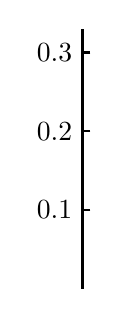
\begin{tikzpicture}[thick]
\draw(0,0.3)--(0,3.6);
\draw(0.1,1.3)--(0,1.3)node[left]{$0.1$}
(0.1,2.3)--(0,2.3)node[left]{$0.2$}
(0.1,3.3)--(0,3.3)node[left]{$0.3$};
\end{tikzpicture}}
\subfloat[$b(10,0,2)$的线条图(右偏)]{
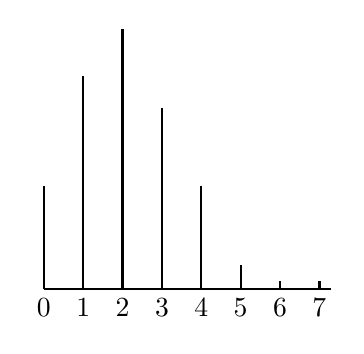
\begin{tikzpicture}[thick,xscale=0.5]
\draw(0,0)node[below]{$0$}--(0,1.3)(1,0)node[below]{$1$}--(1,2.7)
(2,0)node[below]{$2$}--(2,3.3)(3,0)node[below]{$3$}--(3,2.3)
(4,0)node[below]{$4$}--(4,1.3)(5,0)node[below]{$5$}--(5,0.3)
(6,0)node[below]{$6$}--(6,0.1)(7,0)node[below]{$7$}--(7,0.1);
\draw(0,0)--(7.3,0);
\end{tikzpicture}
}\hfill
\subfloat[$b(10,0,5)$的线条图(对称)]{
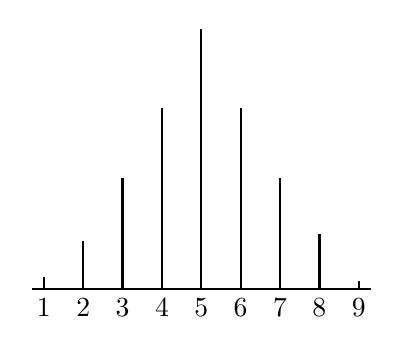
\begin{tikzpicture}[thick,xscale=0.5]
\draw(1,0)node[below]{$1$}--(1,0.15)(2,0)node[below]{$2$}--(2,0.6)
(3,0)node[below]{$3$}--(3,1.4)(4,0)node[below]{$4$}--(4,2.3)
(5,0)node[below]{$5$}--(5,3.3)(6,0)node[below]{$6$}--(6,2.3)
(7,0)node[below]{$7$}--(7,1.4)(8,0)node[below]{$8$}--(8,0.7)
(9,0)node[below]{$9$}--(9,0.1);
\draw(0.7,0)--(9.3,0);
\end{tikzpicture}
}\hfill
\subfloat[$b(10,0,8)$的线条图(左偏)]{
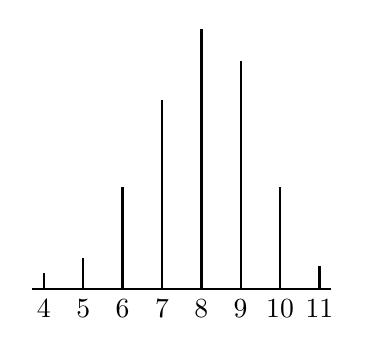
\begin{tikzpicture}[thick,xscale=0.5]
\draw(4,0)node[below]{$4$}--(4,0.2)(5,0)node[below]{$5$}--(5,0.4)
(6,0)node[below]{$6$}--(6,1.3)(7,0)node[below]{$7$}--(7,2.4)
(8,0)node[below]{$8$}--(8,3.3)(9,0)node[below]{$9$}--(9,2.9)
(10,0)node[below]{$10$}--(10,1.3)(11,0)node[below]{$11$}--(11,0.3);
\draw(3.7,0)--(11.3,0);
\draw[very thick](8,0)--(8,3.3);
\end{tikzpicture}
}
  \caption{二项分布$b(n,p)$的线条图\label{fig2.4.1}}
\end{figure}

从上图可以看出

\begin{itemize}
  \item 位于均值$np$附近概率较大;

  \item 随着$p$的增加,分布的峰逐渐右移.
\end{itemize}

\begin{example}
  甲、乙两棋手约定进行10局比赛,以赢的局数多者为胜.设在每局中甲赢的概率为0.6,乙赢的概率为0.4.如果各局比赛是独立进行的,试问甲胜、乙胜、不分胜负的概率各为多少?
\end{example}
\begin{solution}
  以$X$表示10局比赛中甲赢的局数,则$X\sim b(10,0.6)$. 所以
  \begin{align*}
    & P(\text{ 甲胜 } ) = P(X \ge 6 ) = \sum_{k=6}^{10} \Binom{10}k 0.6^k0.4^{10-k} = 0.6330, \\
    & P(\text{ 乙胜 }) = P(X \le 4 ) = \sum_{k=0}^{4} \Binom{10}k 0.6^k0.4^{10-k} = 0.1663 ,\\
    & P(\text{ 不分胜负 }) = P(X = 5) = \Binom{10}5 0.6^50.4^5 = 0.2007.
  \end{align*}

  可见甲胜的可能性达63.3\%,而乙胜的可能性只有16.63\%,它比不分胜负的可能性还要小.最后两个概率之和0.3670表示乙不输的概率.
\end{solution}

\subsection{泊松分布}

\subsubsection{泊松分布}
\textbf{泊松分布}\index{L!离散分布!泊松分布}是1837年由法国数学家泊松(Poisson S.D.1781-1840)首次提出
的. 泊松分布的概率分布列是
\begin{equation}\label{eq2.4.3}
  P(X = k) = \frac{\lambda^k}{k!}\ee^{-\lambda},\; k = 0,1,2,\cdots,
\end{equation}
其中参数$\lambda>0$,记为$X\sim P(\lambda)$.

对泊松分布而言,很容易验证其和为1:
\[
  \sum_{k=0}^{+\infty} \frac{\lambda^k}{k!}\ee^{-\lambda} = \ee^{-\lambda}
  \sum_{k=0}^{+\infty} \frac{\lambda^k}{k!} = \ee^{-\lambda}\ee^\lambda = 1.
\]

泊松分布是一种常用的离散分布,它常与单位时间(或单位面积、单位产品等)上的计数过程相联系,譬如,

\begin{itemize}
  \item 在单位时间内,电话总机接到用户呼唤的次数;

  \item 在单位时间内,一电路受到外界电磁波的冲击次数;

  \item 1平方米内,玻璃上的气泡数;

  \item 一铸件上的砂眼数;

  \item ·在单位时间内,某种放射性物质分裂到某区域的质点数,等等. 都服从泊松分布.因此泊松分布的应用面是十分广泛的.
\end{itemize}

\subsubsection{泊松分布的数学期望和方差}
设随机变量$X\sim P(\lambda)$,则
\[
  E(X) = \sum_{k=0}^{+\infty} k\frac{\lambda^k}{k!}\ee^{-\lambda} = \lambda\ee^{-\lambda}
  \sum_{k=1}^{+\infty}\frac{\lambda^{k-1}}{(k-1)!} = \lambda\ee^{-\lambda} \ee^\lambda = \lambda.
\]

这表明:\textbf{泊松分布$P(\lambda)$的数学期望就是参数$\lambda$}.

又因为
\begin{align*}
  E(X^2) & = \sum_{k=0}^{+\infty} k^2\frac{\lambda^k}{k!}\ee^{-\lambda} =
    \sum_{k=1}^{+\infty}k\frac{\lambda^k}{(k-1)!}\ee^{-\lambda} \\
    & = \sum_{k=1}^{+\infty}[(k-1)+1]\frac{\lambda^k}{(k-1)!}\ee^{-\lambda} \\
    & = \lambda^2\ee^{-\lambda} \sum_{k=2}^{+\infty}\frac{\lambda^{k-2}}{(k-2)!} +
      \lambda\ee^{-\lambda}
    \sum_{k=1}^{+\infty}\frac{\lambda^{k-1}}{(k-1)!} \\
    & = \lambda^2 + \lambda.
\end{align*}

由此得$X$的方差为
\[
  \Var(X) = E(X^2) - [E(X)]^2 = \lambda^2 + \lambda - \lambda^2 = \lambda.
\]
也就是说,泊松分布$P(\lambda)$中的参数A既是数学期望又是方差.

为了看出不同的$\lambda$的值,其泊松分布$P(\lambda)$的变化情况,表 \ref{tab2.4.2} 给出了$\lambda=
0.8,2.0,4.0$时,泊松分布的概率值,其线条图见图 \ref{fig2.4.2}.

\begin{table}[!ht]
  \caption{一些泊松分布的概率值\label{tab2.4.2}}
  \[
    \begin{array}{c|*{11}{c}}
      \toprule
        k & 0 & 1 & 2 & 3 & 4 & 5 & 6 & 7 & 8 & 9 & 10 \\
      \midrule
        P(0.8) & 0.449 & 0.360 & 0.144 & 0.038 & 0.008 & 0.001 & & & & & \\
        P(2.0) & 0.135 & 0.271 & 0.271 & 0.180 & 0.090 & 0.036 & 0.012 & 0.004 & 0.001 &  &  \\
        P(4.0) & 0.018 & 0.074 & 0.146 & 0.195 & 0.196 & 0.156 & 0.104 & 0.060 & 0.030 & 0.013 & 0.005 \\
      \bottomrule
    \end{array}
  \]
\end{table}

\begin{figure}[!ht]
  \centering
\raisebox{0.45cm}{\begin{tikzpicture}[thick]
\draw(0,0)--(0,4.3);
\draw(0.1,1)--(0,1)node[left]{$0.1$}
(0.1,2)--(0,2)node[left]{$0.2$}
(0.1,3)--(0,3)node[left]{$0.3$}
(0.1,4)--(0,4)node[left]{$0.4$};
\end{tikzpicture}}
\subfloat[$P(0.8)$的线条图]{
\begin{tikzpicture}[thick,xscale=0.5]
\draw(0,0)node[below]{$0$}--(0,4.3)(1,0)node[below]{$1$}--(1,3.4)
(2,0)node[below]{$2$}--(2,1.6)(3,0)node[below]{$3$}--(3,0.3)
(4,0)node[below]{$4$}--(4,0.15)(5,0)node[below]{$5$}--(5,0.1);
\draw(0,0)--(5.3,0);
\end{tikzpicture}
}\hfill
\subfloat[$P(2.0)$的线条图]{
\begin{tikzpicture}[thick,xscale=0.5]
\draw(0,0)node[below]{$0$}--(0,1.2)
(1,0)node[below]{$1$}--(1,2.6)(2,0)node[below]{$2$}--(2,2.6)
(3,0)node[below]{$3$}--(3,1.8)(4,0)node[below]{$4$}--(4,1)
(5,0)node[below]{$5$}--(5,0.3)(6,0)node[below]{$6$}--(6,0.1)
(7,0)node[below]{$7$}--(7,0.1);
\draw(-0.3,0)--(7.3,0);
\end{tikzpicture}
}\hfill
\subfloat[$b(10,0,8)$的线条图(左偏)]{
\begin{tikzpicture}[thick,xscale=0.5]
\draw(0,0)node[below]{$0$}--(0,0.2)
(1,0)node[below]{$1$}--(1,0.8)(2,0)node[below]{$2$}--(2,1.6)
(3,0)node[below]{$3$}--(3,1.9)
(4,0)node[below]{$4$}--(4,1.9)(5,0)node[below]{$5$}--(5,1.7)
(6,0)node[below]{$6$}--(6,1.4)(7,0)node[below]{$7$}--(7,0.7)
(8,0)node[below]{$8$}--(8,0.3)(9,0)node[below]{$9$}--(9,0.15);
\draw(-0.3,0)--(9.3,0);
\end{tikzpicture}
}
  \caption{泊松分布$P(\lambda)$的线条图}\label{fig2.4.2}
\end{figure}

从上图可以看出

\begin{itemize}
  \item 位于均值$\lambda$附近概率较大;

  \item 随着$\lambda$的增加,分布逐渐趋于对称.
\end{itemize}

\begin{example}
  一铸件的砂眼(缺陷)数服从参数为$\lambda=0.5$的泊松分布,试求此铸件上至多有1个砂眼(合格品)的概率和至少有2个砂眼(不合格品)的概率,
\end{example}

\begin{solution}
  以$X$表示这种铸件的砂眼数,由题意知$X\sim P(0.5)$.则此种铸件上至多有1个砂眼的概率为
  \[
    P(X \le 1 ) = \frac{0.5^0}{0!}\ee^{-0.5} + \frac{0.5^1}{1!}\ee^{-0.5} = 0.91.
  \]

  至少有2个砂眼的概率为
  \[
    P(X \ge 2) = 1 - P(X \le 1 ) = 0.09.
  \]
\end{solution}

\begin{example}
  某商店出售某种商品,由历史销售记录分析表明,月销售量(件)服从参数为8的泊松分布,问在月初进货时,需要多少库存量,才能有90\%的把握可以满足顾客的需求.
\end{example}
\begin{solution}
  以$X$表示这种商品的月销售量,则$X\sim P(8)$. 那么满足要求的是使下式成立的最小正整数$n$.
  \[
    P(X \le n ) \ge 0.90.
  \]
  为了寻求此种$n$,可以利用泊松分布表,附表1对各种$\lambda$的值,给出了泊松分布函数$P(X\le x)=\sum_{k=0}^{n}\frac{\lambda^k}{k!}\ee^{-\lambda}$的数值表. 在$\lambda=8$时,可从附表1中查得
  \[
    P(X \le 11) = 0.888,\; P(X\le 12 ) = 0.936.
  \]
  所以月初进货12(件)时,能满足93.6\%的顾客的需求.
\end{solution}

\subsubsection{二项分布的泊松近似}
泊松分布还有一个非常实用的特性,即可以用泊松分布作为二项分布的一种近似.在二项分布$b(n,p)$中,当$n$较大时,计算量是令人烦恼的. 而在$p$较小时使用以下的泊松定理,可以减少二项分布中的计算量.

\begin{theorem}{泊松定理}{2.4.1}\index{D!定理!泊松定理}在$n$重伯努利试验中,记事件$A$在一次试验中发生的概率为$p_n$(与试验次数$n$有关),如果当$n\to+\infty$时,有$np_n\to\lambda$,则
\begin{equation}\label{eq2.4.4}
  \lim_{n\to+\infty} \Binom nk p_n^k(1-p_n)^{n-k}
  = \frac{\lambda^k}{k!}\ee^{-\lambda}.
\end{equation}
\end{theorem}

\begin{proof}
  记$np_n=\lambda_n$,记$p_n=\lambda_n/n$,我们可得
  \begin{align*}
    \Binom nk p_n^k(1-p_n)^{n-k} & = \frac{n(n-1)\cdots(n-k+1)}{k!}\left( \frac{\lambda_n}n \right)^k \left( 1 - \frac{\lambda_n}n \right)^{n-k} \\
    & = \frac{\lambda_n^k}{k!}\left( 1 - \frac1n \right)\left( 1 - \frac2n \right) \cdots
    \left( 1 - \frac{k-1}n \right)
    \left( 1 - \frac{\lambda_n}n \right)^{n-k}.
  \end{align*}
  对固定的$k$有
  \begin{align*}
    & \lim_{n\to+\infty}\lambda_n = \lambda ;
    & \lim_{n\to+\infty}\left( 1 - \frac{\lambda_n}n \right)^{n-k} = \ee^{-\lambda} ;
    & \lim_{n\to+\infty}\left( 1 - \frac1n \right) \cdots \left( 1 - \frac{k-1}n \right) = 1.
  \end{align*}
  从而
  \[
    \lim_{n\to+\infty} \Binom nk p_n^k(1-p_n)^{n-k}  = \frac{\lambda^k}{k!}\ee^{-\lambda}
  \]
  对任意的$k$($k=0,1,2,\cdots$)成立. 定理得证.
\end{proof}

由于泊松定理是在$np_n\to\lambda$条件下获得的,故在计算二项分布$b(n,p)$时,当$n$很大,$p$很小,而乘积$\lambda=np$大小适中时,可以用泊松分布作近似,即
\begin{equation}\label{eq2.4.5}
  \Binom nk p_n^k(1-p_n)^{n-k} \approx \frac{(np)^k}{k!}\ee^{-np},\; k=0,1,2,\cdots.
\end{equation}

表 \ref{tab2.4.3} 给出了按二项分布直接计算与利用泊松分布作近似的一些具体数据. 从表中可以看出,两者的结果是很接近的,而且当n愈大和p意小时,近似程度越好.

\begin{table}[!ht]
  \centering
  \caption{二项分布与泊松近似的比较\label{tab2.4.3}}\renewcommand\arraystretch{1.3}
  \begin{tabular}{c|*{4}{c|}c}
    \toprule
      & \multicolumn{4}{c|}{\makecell{二项分布 \\ 按$\mathrm C_n^kp^k(1-p)^{n-k}$计算} } & \makecell{泊松近似 \\ 按$\frac{(np)^k}{k!}\ee^{-np}$计算} \\
      \cmidrule{2-6}
     $k$ & \makecell{$n=10$ \\ $p=0.1$} &  \makecell{$n=20$ \\ $p=0.05$} &
     \makecell{$n=40$ \\ $p=0.025$} &
     \makecell{$n=100$ \\ $p=0.01$} & $\lambda=np=1$ \\
     \midrule
     0 & 0.349 & 0.358 & 0.363 & 0.366 & 0.368 \\
     1 & 0.385 & 0.377 & 0.372 & 0.370 & 0.368 \\
     2 & 0.194 & 0.189 & 0.186 & 0.185 & 0.184 \\
     3 & 0.057 & 0.060 & 0.060 & 0.061 & 0.061 \\
     4 & 0.011 & 0.013 & 0.014 & 0.015 & 0.004 \\
  $>4$ & 0.004 & 0.003 & 0.005 & 0.003 & 0.004 \\
     \bottomrule
  \end{tabular}
\end{table}

以下给出一些利用泊松分布作近似计算的例子.
\begin{example}
  已知某种疾病的发病率为0.001,某单位共有5000人.问该单位患有这种疾病的人数不超过5人的概率为多少?
\end{example}

\begin{solution}
  设该单位患有这种疾病的人数为$X$,则有$X\sim b(5000,0.001)$,而我们所求的为
  \[
    P(X \le 5) = \sum_{k=0}^5\Binom{5000}k 0.001^k0.999^{5000-k},
  \]
  这个概率的计算量很大.由于$n$很大,$p$很小,且$\lambda=np=5$.所以用泊松近似得
  \[
    P(X \le 5) \approx \sum_{k=0}^5\frac{5^k}{k!}\ee^{-5} = 0.616.
  \]
\end{solution}

\begin{solution}
  有10000名同年龄段且同社会阶层的人参加了某保险公司的一
项人寿保险.每个投保人在每年初需交纳200元保费,而在这一年中若投保人死亡,则受益人可从保险公司获得100000元的赔偿费.据生命表知这类人的年死亡率为0.001.试求保险公司在这项业务上

  \begin{inparaenum}[(1)]
    \item 亏本的概率.

    \item 至少获利500000元的概率.
  \end{inparaenum}
\end{solution}

\begin{solution}
  设$X$为10000名投保人在一年中死亡的人数,则$X$服从二项分布$b(10000,0.001)$.保险公司在这项业务上一年的总收人为$200\times10000=
2000000$(元).因为$n=10000$很大,$p=0.001$很小,所以用$\lambda=np=10$的泊松分布进行近似计算.

\begin{inparaenum}[(1)]
  \item 保险公司在这项业务上“亏本”就相当于$\{X>20\}$. 因此所求概率为
      \[
        P(X > 20) = 1 - P(X \le 20) \approx 1 - \sum_{k=0}^{20} \frac{10^k}{k!}\ee^{-10} = 1 - 0.998 = 0.002.
      \]
      由此可看出,保险公司在这项业务上亏本的可能性是微小的.

  \item 保险公司在这项业务上“至少获利500000元”就相当于是$\{X\le15\}$.因此所求概率为
      \[
        P(X \le 15) \approx \sum_{k=0}^{15} \frac{20^k}{k!}\ee^{-10} = 0.951.
      \]
      由此可看出,保险公司在这项业务上至少获利500000元的可能性很大.
\end{inparaenum}
\end{solution}

\begin{example}
  为保证设备正常工作,需要配备一些维修工.如果各台设备发生故障是相互独立的,且每台设备发生故障的概率都是0.01.试在以下各种情况下,求设备发生故障而不能及时修理的概率.

  \begin{inparaenum}[(1)]
    \item\label{ex2.4.8.1} 一名维修工负责20台设备.

    \item\label{ex2.4.8.2} 3名维修工负责90台设备.

    \item 10名维修工负责500台设备.
  \end{inparaenum}
\end{example}

\begin{solution}
  \begin{inparaenum}[(1)]
    \item 以$X_1$表示20台设备中同时发生故障的台数,则$X_1\sim b(20,0.01)$. 用参数为$\lambda=np=20\times0.01=0.2$的泊松分布作近似计算,得所求概率为
        \[
          P(X_1 > 1) \approx 1 - \sum_{k=0}^1\frac{0.2^k}{k!}\ee^{-0.2} = 1 - 0.982 = 0.018.
        \]

    \item 以$X_2$表示90台设备中同时发生故障的台数,则$X_2\sim b(90,0.01)$.用参数为$\lambda=np=90\times0.01=0.9$的泊松分布作近似计算,得所求概率为
        \[
          P(X_2 > 3) \approx 1 - \sum_{k=0}^3\frac{0.9^k}{k!}\ee^{-0.9} = 1 - 0.0987 = 0.013.
        \]

        注意,此种情况下,不但所求概率比 (\ref{ex2.4.8.1}) 中有所降低,而且3名维修工负责90台设备相当于每个维修工负责30台设备,工作效率是 (\ref{ex2.4.8.1}) 中的1.5倍.

    \item 以$X_3$表示500台设备中同时发生故障的台数,则$X_3\sim b(500,0.01)$.用参数为$\lambda=np=500\times0.01=5$的泊松分布作近似计算,得所求概率为
        \[
          P(X_3 > 10) \approx 1 - \sum_{k=0}^{10} \frac{5^k}{k!}\ee^{-5} = 1 - 0.0986 = 0.014.
        \]

        注意,此种情况下所求概率与 (\ref{ex2.4.8.2}) 中基本上一样,而10名维修工负责500台设备相当于每个维修工负责50台设备,工作效率是 (\ref{ex2.4.8.2}) 中的1.67倍,是 (\ref{ex2.4.8.1}) 中的2.5倍.
  \end{inparaenum}

  由此可知:若干维修工共同负责大量设备的维修,将提高工作的效率.
\end{solution}

\subsection{超几何分布}
\subsubsection{超几何分布}
从一个有限总体中进行不放回抽样常会遇到超几何分布.

设有$N$个产品,其中有$M$个不合格品.若从中不放回地随机抽取$n$个,则其中含有的不合格品的个数$X$服从超几何分布,记为$X\sim h(n,N,M)$.超几何分布的概率分布列为(见第 \ref{chap1} 章中例 \ref{exam1.2.3})
\begin{equation}\label{eq2.4.6}
  P(X = k) = \frac{\binom Mk \binom{N-M}{n-k}} {\binom Nn},\; k = 0,1,\cdots,r,
\end{equation}
其中$r=\min\{M,n\}$,且$M\le N,n\le N,n,N,M$均为正整数.

若要验证以上给出的确实为一个概率分布列,只须注意到有组合等式(见习题 \ref{xiti1.2})
\[
   \sum_{k=0}^r \Binom Mk \Binom{N-M}{n-k} = \Binom Nn
\]
即可.

超几何分布是一种常用的离散分布,它在抽样理论中占有重要地位.

\subsubsection{超几何分布的数学期望和方差}
若$X\sim h(n,N,M)$,则$X$的数学期望为
\[
  E(X) = \sum_{k=0}^rk\frac{\binom Mk \binom{N-M}{n-k}} {\binom Nn} = n\frac MN \sum_{k=1}^r \frac{\binom {M-1}{k-1} \binom{N-M}{n-k}} {\binom {N-1}{n-1}} = n\frac MN.
\]
又因为
\begin{align*}
  E(X^2) & = \sum_{k=1}^rk^2\frac{\binom Mk \binom{N-M}{n-k}} {\binom Nn} =
  \sum_{k=2}^r k(k-1) \frac{\binom Mk \binom{N-M}{n-k}} {\binom Nn} + n \frac MN \\
  & = \frac{M(M-1)}{\binom Nn} \sum_{k=2}^rk(k-1) \Binom{M-2}{k-2} \Binom{N-M}{n-k} + n\frac MN \\
  & = \frac{M(M-1)}{\binom Nn} \Binom{N-2}{n-2} + n \frac MN = \frac{M(M-1)n(n-1)}{N(N-1)} + n \frac MN,
\end{align*}
由此得$X$的方差为
\[
  \Var(X) = E(X^2) - [E(X)]^2 = \frac{nM(N-M)(N-n)}{N^2(N-1)} .
\]

\subsubsection{超几何分布的二项近似}
当$n\ll N$时,即抽取个数$n$远小于产品总数$N$时,每次抽取后,总体中的不合格品率$p=M/N$改变甚徽,所以不放回抽样可近似地看成放回抽样,这时超几何分布可用二项分布近似:
\begin{equation}\label{eq2.4.7}
  \frac{\binom Mk \binom{N-M}{n-k}} {\binom Nn}
  \cong \Binom nkp^k(1-p)^{n-k},\;\text{其中}\,p = \frac MN.
\end{equation}

\subsection{几何分布与负二项分布}
\subsubsection{几何分布}
在伯努利试验序列中,记每次试验中事件$A$发生的概率为$p$,如果$X$为事件$A$首次出现时的试验次数,则$X$的可能取值为$1,2,\cdots$,称$X$服从\textbf{几何分布},\index{L!离散分布!几何分布}记为$X\sim Ge(p)$,其分布列为
\begin{equation}\label{eq2.4.8}
  P(X = k) = (1 - p)^{k-1}p,\; k = 1,2,\cdots.
\end{equation}

实际中有不少随机变量服从几何分布,譬如,

\begin{itemize}
  \item 某产品的不合格率为0.05,则首次查到不合格品的检查次数$X\sim Ge(0.05)$;

  \item 某射手的命中率为0.8,则首次击中目标的射击次数$Y\sim Ge(0.8)$;

  \item 掷一颗骰子,首次出现6点的投掷次数$Z\sim Ge(1/6)$;

  \item 同时掷两颗骰子,首次达到两个点数之和为8的投掷次数$W\sim Ge(5/36)$.
\end{itemize}

\subsubsection{几何分布的数学期望和方差}
设随机变量$X$服从几何分布$Ge(p)$,令$q=1-p$,利用逐项微分可得$X$的数学期望为
\begin{align*}
  E(X) & = \sum_{k=1}^{+\infty} kpq^{k-1} = p\sum_{k=1}^{+\infty}kq^{k-1} = p\sum_{k=1}^{+\infty}\frac{\mathrm dq^k}{\mathrm dq} \\
  & = p\frac{\mathrm d}{\mathrm dq}\Big( \sum_{k=0}^{+\infty}q^k \Big) = p \frac{\mathrm d}{\mathrm dq}\left( \frac1{1-q} \right) =
  \frac p{(1-q)^2} = \frac1p.
\end{align*}
又因为
\begin{align*}
  E(X^2) & = \sum_{k=1}^{+\infty} k^2pq^{k-1} = p
  \bigg[ \sum_{k=1}^{+\infty} k(k-1)q^{k-1} + \sum_{k=1}^{+\infty} kq^{k-1} \bigg] \\
  & = pq\sum_{k=1}^{+\infty} k(k-1)q^{k-2} + \frac1p = pq \sum_{k=1}^{+\infty}\frac{\mathrm d^2}{\mathrm dq^2}q^k + \frac1p \\
  & = pq\frac{\mathrm d^2}{\mathrm dq^2}\Big(\sum_{k=1}^{+\infty}q^k\big) + \frac1p
    = pq \frac{\mathrm d^2}{\mathrm dq^2}\left( \frac1{1-q}\right) + \frac1p \\
  & = pq\frac2{(1-q)^3} + \frac1p = \frac{2q}{p^2} + \frac1p,
\end{align*}
由此得$X$的方差为
\[
  \Var(X) = E(X^2) - [E(X)]^2 = \frac{2q}{p^2} + \frac1p - \frac1{p^2} = \frac{1-p}{p^2}.
\]

\subsubsection{几何分布的无记忆性}
\begin{theorem}{几何分布的无记忆性}{2.4.2}
  设$X\sim Ge(p)$,则对任意正整数$m$与$n$有
  \begin{equation}\label{eq2.4.9}
    P(X > m + n| X > m) = P(X > n).
  \end{equation}
\end{theorem}

在证明之前先解释上述概率等式的含义.在一列伯努利试验序列中,若首次成功$(A)$出现的试验次数X服从几何分布,则事件“$X>m$”表示前$m$次试验中$A$没有出现.假如在接下去的$n$次试验中$A$仍未出现,这个事件记为“$X>m+n$”.这个定理表明:在前$m$次试验中$A$没有出现的条件下,则在接下去的$n$次试验中$A$仍未出现的概率只与$n$有关,而与以前的$m$次试验无关,似乎忘记了前$m$次试验结果,这就是无记忆性.
\begin{proof}
  因为
  \[
    P(X > n) = \sum_{k=n+1}^{+\infty}(1-p)^{k-1}p = \frac{p(1-p)^n}{1-(1-p)} = (1-p)^n,
  \]
  所以对任意的正整数$m$与$n$,条件概率
  \begin{align*}
    P(X > m + n | X > m) & = \frac{P(X>m+n)}{P(X>m)} = \frac{(1-p)^{m+n}}{(1-p)^m} \\
    & = (1 - p)^n = P(X > n).
  \end{align*}
  这就证得了 \eqref{eq2.4.9} 式.
\end{proof}

\subsubsection{负二项分布}
作为几何分布的一种延伸,我们注意下面的\textbf{负二项分布},\index{L!离散分布!负二项分布}亦称\textbf{巴斯卡分布}:

在伯努利试验序列中,记每次试验中事件$A$发生的概率为$p$,如果$X$为事件$A$第$r$次出现时的试验次数,则$X$的可能取值为$r,r+1,\cdots,r+m,\cdots$. 称$X$服从\textbf{负二项分布}\index{L!离散分布!负二项分布}或\textbf{巴斯卡分布}\index{L!离散分布!巴斯卡分布},其分布列为
\begin{equation}\label{eq2.4.10}
  P(X = k) = \Binom{k-1}{r-1} p^r(1-p)^{k-r},\; k=r,r+1,\cdots.
\end{equation}
记为$X\sim Nb(r,p)$. 当$r=1$时,即为几何分布.

这是因为在次伯努利试验中,最后一次一定是$A$,而前$k-1$次中$A$应出现$r-1$次,由二项分布知其概率为$\binom{k-1}{r-1}p^{r-1}(1-p)^{k-r}$,再乘以最后一次出现$A$的概率$p$,即得 \eqref{eq2.4.10}.

可以算得负二项分布的数学期望为$r/p$,方差为$r(1-p)/p^2$.从直观上看这是合理的,因为首次出现$A$的平均试验次数是$1/p$,那么第$r$个$A$出现所需的平均试验次数是$r/p$.

如果将第一个$A$出现的试验次数记为$X_1$,第二个$A$出现的试验次数(从第一个$A$出现之后算起)记为$X_2$,第$r$个$A$出现的试验次数(从第$r-1$个$A$出现之后算起)记为$X_r$,则$X_i$独立同分布,且$X_i\sim Ge(p)$.此时有$X=X_1+X_2+\cdots+X_r\sim Nb(r,p)$,即负二项分布的随机变量可以表示成$r$个独立同分布的几何分布随机变量之和.

\begin{xiti}
  \item 一批产品中有10\%的不合格品,现从中任取3件,求其中至多有一件不合格品的撕率.

  \item 一条自动化生产线上产品的一级品率为0.8,现检查5件,求至少有2件一级品的概率.

  \item 某优秀射手命中10环的概率为0.7,命中9环的概率为0.3.试求该射手三次射击所得的环数不少于29环的概率.

  \item 经验表明:预定餐厅座位而不来就餐的顾客比例为20\%.如今餐厅有50个座位,但预定给了52位顾客,问到时顾客来到餐厅而没有座位的概率是多少?

  \item 设随机变量$X\sim b(n,p)$,已知$E(X)=2.4,\Var(X)=1.44$,求两个参数$n$与$p$各为多少?

  \item 设随机变量$X$服从二项分布$b(2,p)$,随机变量$Y$服从二项分布$b(4,p)$. 若$P(X|ge1)=8/9$,试求$P(Y\ge1)$.

  \item 一批产品的不合格品率为0.02,现从中任取40只进行检查,若发现两只或两只以土不合格品就拒收这批产品.分别用以下方法求拒收的概率:\begin{inparaenum}[(1)]\item 用二项分布作精确计算;\item 用泊松分布作近似计算.
      \end{inparaenum}

  \item 设$X$服从泊松分布,且已知$P(X=1)=P(X=2)$,求$P(X=4)$.

  \item 已知某商场一天来的顾客数$X$服从参数为$\lambda$的泊松分布,而每个来到商场的顾客购物的概率为$p$,证明:此商场一天内购物的顾客数服从参数为$\lambda p$的泊松分布.

  \item 从一个装有$m$个白球、$n$个黑球的袋中返回地摸球,直到摸到白球时停止.试求取出黑球数的期望.

  \item 某种产品上的缺陷数$X$服从下列分布列:
  \[
    P(X = k) = \frac1{2^{k+1}},\; k = 0,1,\cdots,
  \]
  求此种产品上的平均缺陷数.

  \item 设随机变量$X$的密度函数为
  \[
    p(x) = \begin{cases}
      2x, & 0<x<1; \\
      0, & \text{其他}.
    \end{cases}
  \]
  以$Y$表示对$X$的三次独立重复观察中事件$\{X\le1/2\}$出现的次数,试求$P(Y=2)$.

  \item 某产品的不合格品率为0.1,每次随机抽取10件进行检验,若发现其中不合格品数多于1,就去调整设备,若检验员每天检验4次,试同每天平均要调整几次设备.
\end{xiti}

\section{常用连续分布}
\subsection{正态分布}
正态分布是概率论与数理统计中最重要的一个分布,高斯(Gauss)在研究误差理论时首先用正态分布来刻画误差的分布,所以正态分布又称为高斯分布.本书第四章的中心极限定理表明:一个变量如果是由大量微小的、独立的随机因素的叠加结果,那么这个变量一定是正态变量.因此很多随机变量可以用正态分布描述或近似描述,譬如测量误差、产品重量、人的身高、年降雨量等都可用正态分布描述.

\subsubsection{正态分布的密度函数和分布函数}
若随机变量$X$的密度函数为
\begin{equation}\label{eq2.5.1}
  p(x) = \frac1{\sqrt{2\pi}\sigma} \ee^{-\frac{(x-\mu)^2}{2\sigma^2}},\; -\infty<x<+\infty,
\end{equation}
则称$X$服从\textbf{正态分布}\index{L!连续分布!正态分布},称$X$为\textbf{正态变量},记作$X\sim N(\mu,\sigma^2)$. 其中参数$-\infty<\mu<+\infty,\sigma>0$. 其密度函数$p(x)$的图形如图 \ref{fig2.5.1}(a)所示. $p(x)$是一条钟形曲线,中间高、二边低、左右关于$\mu$对称,$\mu$是正态分布的中心,且在$x=\mu$附近取值的可能性大,在两侧取值的可能性小. $\mu\pm\sigma$是该曲线的拐点.

\begin{figure}[!ht]
  \centering
\subfloat[密度函数$p(x)$]{
\begin{tikzpicture}[semithick,yscale=2,>=Stealth]
\draw[->](-2.7,0)--(0,0)node[below=1pt]{$\mu$}--(2.7,0)node[below]{$x$};
\draw[->](0,0)--(0,1.4)node[right]{$p(x)$};
\draw[samples=100,domain=-2.5:2.5,thick]plot(\x,{e^(-(\x)^2)+0.04});
\draw[dashed](-0.8,{e^(-0.64)+0.04})--(-0.8,0)node[below]{$\mu-\sigma$}
(0.8,{e^(-0.64)+0.04})--(0.8,0)node[below]{$\mu+\sigma$};
\draw(0.8,{e^(-0.64)+0.04})--(-0.8,{e^(-0.64)+0.04});
\end{tikzpicture}
}\hspace{1.5cm}
\subfloat[分布函数$F(x)$]{
\begin{tikzpicture}[semithick,yscale=2,>=Stealth]
\draw[->](-2.7,0)--(0,0)node[below=1pt]{$\mu$}--(2.7,0)node[below]{$x$};
\draw[->](0,0)--(0,1.4)node[right]{$F(x)$};
\draw[samples=100,domain=-2.5:2.5,thick]plot(\x,{(atan(\x))/135+0.55});
\draw[dashed](-2.5,1.1)--(2.5,1.1);
\end{tikzpicture}
}
  \caption{正态分布}\label{fig2.5.1}
\end{figure}

正态分布$N(\mu,\sigma^2)$的分布函数为
\begin{equation}\label{eq2.5.2}
  F(x) = \frac1{\sqrt{2\pi}\sigma}\int_{-\infty}^x \ee^{-\frac{(t-\mu)^2}{2\sigma^2}} \dd t.
\end{equation}
它是一条光滑上升的$S$形曲线,见图 \ref{fig2.5.1}(b).

图 \ref{fig2.5.2} 给出了在$\mu$和$\sigma$变化时,相应正态密度曲线的变化情况.

\begin{itemize}
  \item 从图 \ref{fig2.5.2}(a)中可以看出:如果固定,改变$\mu$的值,则图形沿$x$轴平移,而不改变其形状.也就是说正态密度函数的位置由参数$\mu$所确定,因此亦称$\mu$为\textbf{位置参数}.

  \item 从图 \ref{fig2.5.2}(b)中可以看出:如果固定$\mu$,改变$\sigma$的值,则$\sigma$愈小,曲线呈高而瘦;$\sigma$愈大,曲线呈矮而胖.也就是说正态密度函数的尺度由参数$\sigma$所确定,因此称$\sigma$为\textbf{尺度参数}.
\end{itemize}

\subsubsection{标准正态分布}
称$\mu=0,\sigma=1$时的正态分布$N(0,1)$为标准正态分布.

通常记标准正态变量为$U$,记标准正态分布的密度函数为$\varphi(u)$,分布函数为$\varPhi(u)$,即
\begin{gather*}
  \varphi(u) = \frac1{\sqrt{2\pi}} \ee^{-\frac{u^2}2},\; -\infty < u < +\infty, \\
  \varPhi(u) = \frac1{\sqrt{2\pi}} \int_{-\infty}^u \ee^{-\frac{t^2}2}\dd t,\; -\infty < u < +\infty.
\end{gather*}

由于标准正态分布的分布函数不含任何未知参数,故其值$\varPhi(u)=P(U\le u)$完全可以算出,附表2对$u\ge0$给出了$\varPhi(u)$的值,利用这张表可以算得

\begin{itemize}
  \item $\varPhi(-u)=1-\varPhi(u)$.
  \item $P(U>u)=1-\varPhi(u)$.
  \item $P(a<U<b)=\varPhi(b)-\varPhi(a)$.
  \item $P(|U|<c)=2\varPhi(c)-1$.
\end{itemize}
这些等式都不难推得.

\begin{example}
  设$U\sim N(0,1)$,利用附表2,求下列事件的概率:

  \begin{inparaenum}[(1)]
    \item $P(U<1.52)=\varPhi(1.52)=0.9357$.

    \item $P(U>1.52)=1-\varPhi(1.52)=1-0.9357=0.0642$.

    \item $P(U<-1.52)=1-\varPhi(1.52)=0.0643$.

    \item $P(-0.75\le U\le1.52)=\varPhi(1.52)-\varPhi(-0.75)
        =\varPhi(1.52)-[1-\varPhi(0.75)]=0.9357-1+
        0.7734=0.7091$.

    \item $P(|U|\le1.52)=2\varPhi(1.52)-1=2\times0.9357-1
        =0.8714$.
  \end{inparaenum}
\end{example}

\subsubsection{一般正态分布的标准化}
正态分布有一个家族
\[
  \mathscr P = \{ N(\mu,\sigma^2):-\infty<\mu<+\infty,\sigma>0 \},
\]
标准正态分布$N(0,1)$是其一个成员.实际上很少有随机变量恰好服从标准正态分布.以下定理说明:对一般正态分布都可以通过一个线性变换(标准化)化成标准正态分布. 因此与正态变量有关的一切事件的概率都可通过查标准正态分布函数表获得. 由此可见标准正态分布$N(0,1)$对一般正态分布$N(\mu,\sigma^2)$的计算起着关键的作用.

\begin{theorem}{}{2.5.1}
  若$X\sim N(\mu,\sigma^2)$,则$U=(X-\mu)/\sigma\sim N(0,1)$.
\end{theorem}
\begin{proof}
  记$X$与$U$的分布函数分别为Fx(x)与Fu(u),则由分布函数的定义知
  \begin{align*}
    F_U(u) & = P(U \le u) = P \left( \frac{X - \mu}\sigma \le u \right) \\
    & = P(X \le \mu + \sigma u) = F_X(\mu + \sigma u).
  \end{align*}
  由于正态分布函数是严格单调增函数,且处处可导,因此若记$X$与$U$的密度函数分别为$p_X(x)$与$P_U(u)$,则有
  \[
    P_U(u) = \frac{\mathrm d}{\mathrm du}F_X(\mu + \sigma u) = p_X(\mu+\sigma u)\cdot \sigma = \frac1{\sqrt{2\pi}} \ee^{-u^2/2},
  \]
  由此得
  \[
    U = \frac{X-\mu}\sigma \sim N(0,1).
  \]

  由以上定理,我们马上可以得到一些在实际中有用的计算公式,若$N(\mu,\sigma^2)$,则
  \begin{align}
    & P(X \le c) = \varPhi\left( \frac{c-\mu}\sigma \right) . \label{eq2.5.3}\\
    & P(a < X\le b) = \varPhi\left( \frac{b-\mu}\sigma \right) - \varPhi\left( \frac{a-\mu}\sigma \right).\label{eq2.5.4}
  \end{align}
\end{proof}

\begin{example}
  设随机变量$X$服从正态分布$N(108,3^2)$,试求

  \begin{inparaenum}[(1)]
    \item $P(102<X<117)$;

    \item 常数$a$,使得$P(X<a)=0.95$.
  \end{inparaenum}
\end{example}
\begin{solution}
  利用公式 \eqref{eq2.5.4} 及查附表2得

  \begin{inparaenum}[(1)]
    \item
    \begin{align*}
      P( 102 < X < 117 ) & = \varPhi\left(\frac{117-108}3\right) -
      \varPhi\left( \frac{102-108}3 \right) \\
      & = \varPhi(3) - \varPhi(-2) = \varPhi(3) + \varPhi(2) - 1 \\
      & = 0.9987 + 0.9772 - 1 = 0.9759.
    \end{align*}

    \item
    \[
      P(X < a) = \varPhi\left( \frac{a-108}3 \right) = 0.95, \quad \text{或}\quad
      \varPhi^{-1}().95) = \frac{a-108}3,
    \]
    其中$\varPhi^{-1}$为$\varPhi$的反函数,从附表2由里向外反查得
    \[
      \varPhi(1.64) = 0.9495,\quad \varPhi(1.65) = 0.9505,
    \]
    再用线性内插法可得$\varPhi(1.645)=0.95$,即$\varPhi^{-1}(0.95)=1.645$,故
    \[
      \frac{a - 108}3 = 1.645,
    \]
    从中解得$a=112.935$.
  \end{inparaenum}
\end{solution}

从上例我们可以看出,有些场合下给定$\varPhi(x)$的值,可以从附表2中由里向外反查表来得到$a$的值,这种手段在统计中被大量使用.

\begin{example}
  恒温箱是靠温度调节器根据箱内温度的变化不断进行调整的,所以恒温箱内的实际温度$X$(单位为$^\circ\mathrm C$)是一个随机变量.如果将温度调节器设定在$d^\circ\mathrm C$,且$X\sim N(d,\sigma^2)$,其中$\sigma$反映的是温度调节器的精度.

  \begin{inparaenum}[(1)]
    \item 当$d=90^\circ\mathrm C,\sigma=0.5$时,试求箱内的温度在$89^\circ\mathrm C$至$91^\circ\mathrm C$的概率.

    \item 当$d=90^\circ\mathrm C,\sigma=2$时,试求箱内的温度在$89^\circ\mathrm C$至$91^\circ\mathrm C$的概率.

    \item 当$\sigma=0.5$时,要有95\%的可能性保证箱内温度不低于$90^\circ\mathrm C$,问应将温度调节器设定为多少度为宜?
  \end{inparaenum}
\end{example}

\begin{solution}
  \begin{inparaenum}[(1)]
    \item 随求概率为
    \begin{align*}
      P(89 \le X <91) & = \varPhi\left( \frac{91-90}{0.5} \right) - \varPhi\left( \frac{89-90}{0.5} \right) \\
      & = 2\varPhi(2) - 1 = 2\times0.9772 - 1 = 0.9544.
    \end{align*}
    这说明如果温度调节器的精度$\sigma=0.5$时,箱内温度在$89^\circ\mathrm C$至$91^\circ\mathrm C$的可能性是很大的.

    \item 所求概率为
    \begin{align*}
      P(89 \le X <91) & = \varPhi\left( \frac{91-90}2 \right) - \varPhi\left( \frac{89-90}2 \right) \\
      & = 2\varPhi(0.5) - 1 = 2\times0.6915 - 1 = 0.3830.
    \end{align*}
    这说明如果温度调节器的精度$\sigma=2$时,箱内温度在$89^\circ\mathrm C$至$91^\circ\mathrm C$是较困难的.

    \item 按题意需求$d$满足
    \[
      P(X \ge 90) \ge 0.95,\quad \text{即}\, 1 - \varPhi\left( \frac{90-d}{0.5} \right) \ge 0.95,
    \]
    所以应该有
    \[
      \varPhi\left( \frac{90-d}{0.5} \right) \le 0.05.
    \]
    查附表2得
    \[
      \frac{90 - d}{0.5} \le -1.645,
    \]
    所以
    \[
      d \ge 1.645 \times 0.5 + 90 = 90.8225.
    \]
    故取$d=91^\circ\mathrm C$可满足条件.
  \end{inparaenum}
\end{solution}

\subsubsection{正态分布的数学期望与方善}
设随机变量$X\sim N(\mu,\sigma^2)$,由于$U=(X-\mu)/\sigma\sim N(0,1)$,所以$U$的数学期望为
\[
  E(U) = \frac1{\sqrt{2\pi}}\int_{-\infty}^{+\infty}
  u \ee^{-\frac{u^2}2}\dd u ,
\]
注意到上述积分的被积函数为一个奇函数,所以其积分值等于0,即$E(U)=0$. 又因为$X=\mu+\sigma U$,所以由数学期望的线性性得
\[
  E(X) = \mu + \sigma \times 0 = \mu.
\]
也就是说,正态分布$N(\mu,\sigma^2)$中$\mu$为数学期望.

又因为
\begin{align*}
  \Var(U) & = E(U^2) = \frac1{\sqrt{2\pi}}\int_{-\infty}^{+\infty}
  u^2 \ee^{-\frac{u^2}2}\dd u \\
  & = \frac1{\sqrt{2\pi}}\int_{-\infty}^{+\infty}
  u^2 \ee^{-\frac{u^2}2}\dd u \\
  & \frac1{\sqrt{2\pi}} \left( -u\ee^{-\frac{u^2}2}\Big|_{-\infty}^{+\infty}
  + \int_{-\infty}^{+\infty}\ee^{-\frac{u^2}2} \dd u \right) \\
  & = \frac1{\sqrt{2\pi}}\int_{-\infty}^{+\infty}
   \ee^{-\frac{u^2}2}\dd u = \frac1{\sqrt{2\pi}} \sqrt{2\pi} = 1.
\end{align*}
因为$X=\sigma U+\mu$,所以由方差的性质得
\[
  \Var(X) = \Var(\sigma U + \mu) = \sigma^2.
\]
这说明,正态分布$N(\mu,\sigma^2)$中另一个参数$\sigma^2$就是方差.

在求正态分布的数学期望和方差中,用到了一种变换:令$U=(X-\mu)/\sigma$,由$E(U)=0,\Var(U)=1$,然后再去求出$X$的数学期望和方差.这个变换具有普遍意义,也就是对任意随机变量$X$,如果$X$的数学期望为$\mu$,方差为$\sigma^2$,则称
\[
  X^\ast = \frac{X - \mu}\sigma
\]
为$X$的\textbf{标准化随机变量},且可得
\[
  E(X^\ast) = 0,\quad \Var(X^\ast) = 1.
\]

\subsubsection{正态分布的$3\sigma$原则}
设$X\sim N(\mu,\sigma^2)$,则
\begin{equation}\label{eq2.5.5}
  P(|X - \mu|<k\sigma) = \varPhi(k) - \varPhi(-k) = \begin{cases}
    0.6826, & k = 1; \\
    0.9545, & k = 2; \\
    0.9973, & k = 3
  \end{cases}.
\end{equation}

从上式中可以看出:尽管正态变量的取值范围是$(-\infty,+\infty)$,但它的99.73\%的值落在$\mu-3\sigma,\mu+3\sigma$内. 这个性质被实际工作者称作是正态分布的“$3\sigma$原则”. 正态分布的$3\sigma$原则在实际工作中很有用,工业生产上用的控制图,和一些产品质量指数(如$C_p,C_{pk}$)都是根据$3\sigma$原则制定的.

\subsection{均匀分布}
\subsubsection{均匀分布的密度函数和分布函数}
若随机变量X的密度函数(见图 \ref{fig2.5.3}(a))为
\begin{equation}\label{eq2.5.6}
  p(x) = \begin{cases}
    \frac1{b-a}, & a < x < b ; \\
    0, & \text{其他}.
  \end{cases}
\end{equation}
则称$X$服从区间$(a,b)$上的\textbf{均匀分布},\index{L!连续分布!均匀分布}记作$X\sim U(a,b)$,其分布函数(见图 \ref{fig2.5.3}(b))为
\begin{equation}\label{eq2.5.7}
  F(x) = \begin{cases}
    0, & x < a ; \\
    \frac{x-a}{b-a}, & a \le x < b; \\
    1, & x \ge b.
  \end{cases}
\end{equation}

\begin{figure}[!ht]
  \centering
\subfloat[密度函数$p(x)$]{
\begin{tikzpicture}[semithick,>=Stealth,samples=100,scale=2.5]
\draw[->](0,0)node[below left]{$O$}--(1.7,0)node[below]{$x$};
\draw[->](0,0)--(0,1.2)node[right]{$p(x)$};
\draw[thick](0.3,0.6)--(1.3,0.6);\node[left]at(0,0.6){$\frac1{b-a}$};
\draw[dashed](0.3,0.6)--(0.3,0)node[below]{$a$}
(1.3,0.6)--(1.3,0)node[below]{$b$};
\end{tikzpicture}
}
\subfloat[分布函数$F(x)$]{
\begin{tikzpicture}[semithick,>=Stealth,samples=100,scale=2.5]
\draw[->](0,0)node[below left]{$O$}--(1.7,0)node[below]{$x$};
\draw[->](0,0)--(0,1.2)node[right]{$F(x)$};
\draw[thick](0.3,0)node[below]{$a$}--(1.2,0.9)--(1.7,0.9);
\draw(1.2,0)node[below]{$b$}--(1.2,0.03);
\draw(0,0.9)node[left]{$1$}--(0.03,0.9);
\end{tikzpicture}
}
  \caption{$(a,b)$上的均匀分布}\label{fig:2.5.3}
\end{figure}

均匀分布的背景可视作随机点$X$落在区间$(a,b)$上的位置.均匀分布在实际中经常使用,譬如一个半径为$r$的汽车轮胎,因为轮胎圆周上的任一点接触地面的可能性是相同的,所以轮胎圆周接触地面的位置$X$是服从$(),2\pi r)$上的均匀分布,这只要看一看报度轮胎的四周磨损程度几乎是相同的就可明白均匀分布的含义了.

\begin{example}
  设随机变量$X$服从$(0,10)$上的均匀分布,现对X进行4次独立观测,试求至少有3次观测值大于5的概率.
\end{example}

\begin{solution}
  设随机变量$Y$是4次独立观测中观测值大于5的次数,则$Y\sim b(4,p)$,其中$p=P(X>5)$. 由$X\sim U(0,10)$,知$X$的密度函数
  \[
    p(x) = \begin{cases}
      \frac1{10}, & 0 < x < 10; \\
      0, & \text{其他}.
    \end{cases}
  \]
  所以
  \[
    p = P(X>5) = \int_5^{10} \frac1{10} \dd x = \frac12,
  \]
  于是
  \[
    P(Y\ge3) = \Binom43 p^3(1-p) + \Binom44 = 4\left(\frac12\right)^4 + \left(\frac12\right)^4 = \frac5{16}.
  \]
\end{solution}

\subsubsection{均匀分布的数学期望和方差}
设随机变量$X\sim U(a,b)$,则
\[
  E(X) = \int_a^b \frac x{b-a} \dd x = \frac{b^2-a^2}{2(b-a)} = \frac{a+b}2,
\]
这正是区间$(a,b)$的终点.

又因为
\[
  E(X^2) = \int_a^b\frac{x^2}{b-a} \dd x = \frac{b^3-a^3}{3(b-a)} = \frac{a^2+ab+b^2}3,
\]
由此得$X$的方差为
\[
  \Var(X) = E(X^2) - [E(X)]^2 = \frac{a^2+ab+b^2}3 - \frac{(a+b)^2}4 = \frac{(b-a)^2}{12}.
\]

\subsection{指数分布}
\subsubsection{指数分布的密度函数和分布函数}
若随机变量X的密度函数(见图 \ref{fig2.5.4})为
\begin{equation}\label{eq2.5.8}
  p(x) = \begin{cases}
    \lambda \ee^{-\lambda x}, & x \ge 0; \\
    0, & x < 0,
  \end{cases}
\end{equation}
则称$X$服从\textbf{指数分布},\index{L!连续分布!指数分布}记作$X\sim Exp(\lambda)$,其中参数$\lambda>0$. 指数分布的分布函数为
\begin{equation}\label{eq2.5.9}
  F(x) = \begin{cases}
    1 - \ee^{-\lambda x}, & x \ge 0; \\
    0, & x < 0.
  \end{cases}
\end{equation}

\begin{figure}[!ht]
  \centering
\begin{tikzpicture}[semithick,>=Stealth,samples=100]
\draw[->](0,0)node[below left]{$O$}--(4,0)node[below]{$x$};
\draw[->](0,0)--(0,3.6)node[right]{$p(x)$};
\foreach \x in{1,2,3}
\draw(\x,0)node[below]{$\x$}--(\x,0.08)(0,\x)node[left]{$\x$}--(0.08,\x);
\draw[domain=0:3.6]plot(\x,{e^(-\x)});
\draw[domain=0:3.6](0,0.5)node[left]{$0.5$}--plot(\x,{0.5*e^(-0.5*\x)});
\draw[domain=0:3.6]plot(\x,{3*e^(-3*\x)});
\node[inner sep=0pt](a)at(1,2){$\lambda=3$};
\node[inner sep=0pt](b)at(1.5,1){$\lambda=1$};
\node[inner sep=0pt](c)at(3,0.6){$\lambda=0.5$};
\draw[->](a)--(0.2,{3*e^(-3*0.2)});
\draw[->](b)--(0.85,{e^(-0.85)});
\draw[->](c)--(2.6,{0.5*e^(-0.5*2.6)});
\end{tikzpicture}
  \caption{参数为$\lambda$的指数分布密度函数}\label{fig2.5.4}
\end{figure}

因为指数分布随机变量只可能取非负实数,所以指数分布常被用作各种“寿命”分布,臂如电子元器件的寿命、动物的寿命、电话的通话时间、随机服务系统中的服务时间等都可假定服从指数分布.指数分布在可靠性与排队论中有着广泛的应用.

\subsubsection{指数分布的数学期望和方差}
设随机变量$X\sim Exp(\lambda)$,则
\begin{align*}
  E(X) & = \int_0^{+\infty}x\lambda \ee^{-\lambda x}\dd x = \int_0^{+\infty}x \dd (-\ee^{-\lambda x}) \\
  & = -x\ee^{-\lambda x}\big|_0^{+\infty} + \int_0^{+\infty}\ee^{-\lambda x}\dd x = - \frac1\lambda \ee^{-\lambda x}\bigg|_0^{+\infty} = \frac1\lambda .
\end{align*}
在指数分布中,有时记$\theta=1/\lambda$,则$\theta$为指数分布的数学期望.

又因为
\begin{align*}
  E(X^2) & = \int_0^{+\infty}x^2\lambda \ee^{-\lambda x}\dd x = \int_0^{+\infty}x^2\dd(-\ee^{-\lambda x}) \\
  & = -x^2\ee^{-\lambda}\bigg|_0^{+\infty}  +
    2\int_0^{+\infty} x\ee^{-\lambda x} \dd x = \frac2{\lambda^2},
\end{align*}
由此得$X$的方差为
\[
  \Var(X) = E(X^2) - [E(X)]^2 = \frac2{\lambda^2} - \frac1{\lambda^2} = \frac1{\lambda^2}.
\]

\subsubsection{指数分布的无记忆性}
下面给出指数分布在连续分布类中所特有的一个性质.
\begin{theorem}{指数分布的无记忆性}{2.5.2}
  如果$X\sim Exp(\lambda)$,则对任意$s>0,t>0$,有
  \begin{equation}\label{eq2.5.10}
    P(X > s + t| X > s) = P( X > t).
  \end{equation}
\end{theorem}

上式的含义为:记$X$是某种产品的使用寿命(h),若$X$服从指数分布,那么已知此产品使用了$s$ h没发生故障,则再能使用$t$ h而不发生故障的概率与已使用的$s$ h无关,只相当于重新开始使用$t$ h的概率,即对已使用过的$s$ h没有记忆.

\begin{proof}
  因为$X\sim Exp(\lambda)$,所以$P(X>s)=\ee^{-\lambda s},s>0$. 又因为
  \[
    \{X>s+t\} \subseteq \{ X>s \},
  \]
  于是条件概率
  \[
    P(X>s+t | X>s) = \frac{P(X>s+t)}{P(X>s)} = \frac{\ee^{-\lambda(s+t)}}{\ee^{-\lambda s}} = \ee^{-\lambda t} =P(X>t).
  \]
  这就证明 \eqref{eq2.5.10} 式.
\end{proof}

指数分布的无记忆性与几何分布的无记忆性是类似的.

以下例子说明了泊松分布与指数分布的关系.

\begin{example}
  如果某设备在任何长为$t$的时间$[0,t]$内发生故障的次数$N9t)$服从参数为$\lambda t$的泊松分布,则相继两次故障之间的时间间隔$T$服从参数为$\lambda$的指数分布.
\end{example}

\begin{solution}
  设$N(t)\sim P(\lambda t)$,即
  \[
    P\big( N(t) = k \big) = \frac{(\lambda t)^k}{k!} \ee^{-\lambda t},\quad k=0,1,\cdots.
  \]

  注意到两次故障之间的时间间隔$T$是非负随机变量,且事件$\{T\ge t\}$说明此设备在$[0,t]$内没有发生故障,即$\{T\ge t\}=\{N(t)=0\}$,由此我们得

  当$t<0$时,有$F_T(t)=P(T\le t)=0$;

  当$t\ge0$时,有
  \[
    F_T(t) = P(T\le t) = 1 - P(T>t) = 1 -P\big( N(t)=0 \big) = 1 - \ee^{-\lambda t},
  \]
  所以$T\sim Exp(\lambda)$,相继两次故障之间的时间间隔$T$服从参数为$\lambda$的指数分布.
\end{solution}

\subsection{伽马分布}
\subsubsection{伽马函数}
称以下函数
\begin{equation}\label{eq2.5.11}
  \Gamma(\alpha) = \int_0^{+\infty}x^{\alpha-1}\ee^{-x} \dd x
\end{equation}
为\textbf{伽玛函数},\index{G!伽玛函数},其中参数$\alpha>0$. 伽玛函数具有如下性质:

\begin{inparaenum}[(1)]
  \item $\Gamma(1)=1,\Gamma\left(\frac12\right)=\sqrt\pi$;

  \item $\Gamma(\alpha+1)=\alpha\Gamma(\alpha)$(可用分部积分法证得). 当$\alpha$为自然数$n$时,有
      \[
        \Gamma(n+1) = n\Gamma(n) = n!.
      \]
\end{inparaenum}

\subsubsection{伽玛分布}
若随机变量$X$的密度函数为
\begin{equation}\label{eq2.5.12}
  p(x) = \begin{cases}
    \frac{\lambda^\alpha}{\Gamma(\alpha)}x^{\alpha-1}
    \ee^{-\lambda x}, & x\ge 0 ; \\
    0, & x < 0,
  \end{cases}
\end{equation}
则称$X$服从\textbf{伽玛分布},\index{L!连续分布!伽玛分布}记作$X\sim Ga(\alpha,\lambda)$,其中$\alpha>0$为形状参数,$\lambda>0$为尺度参数. 图 \ref{fig2.5.5} 给出若于条$\lambda$固定、$\alpha$不同的伽玛密度函数曲线,从图中可以看出:

\begin{itemize}
  \item $0<\alpha<1$时,$p(x)$是严格下降函数,且在$x=0$处有奇异点;

  \item $\alpha=1$时,$p(x)$是严格下降函数,且在$x=0$处$p(0)=\lambda$;

  \item $1<\alpha\le2$,$p(x)$是单峰函数,向上凸、后下凸;

  \item $2<\alpha$时,$p(x)$是单峰函数,先下凸、中间上凸、后下凸. 且$\alpha$越大,$p(x)$越近似于正态分布.
\end{itemize}

\begin{figure}[!ht]
  \centering
\subfloat{
\begin{tikzpicture}[semithick,>=Stealth,samples=150,yscale=2,xscale=0.9]
\draw[->](0,0)node[below left]{$O$}--(4.4,0)node[below]{$x$};
\draw[->](0,0)--(0,1.7)node[right]{$p(x)$};
\draw[thick,domain=0.12:2.6]plot(\x,{e^(-\x)/sqrt(\x)/1.77});
\draw[thick,domain=0:3]plot(\x,{e^(-\x)});
\draw[thick,domain=0:4]plot(\x,{2.5*(\x)*e^(-\x)});
\node[inner sep=0pt](a)at(2,0.45){$\alpha=1$};
\node[inner sep=0pt](b)at(1,1.2){$\alpha<1$};
\node[inner sep=0pt](c)at(3,0.8){$\alpha>1$};
\draw[->](a)--(2,{e^(-2)});
\draw[->](b)--(0.2,{e^(-0.2)/sqrt(0.2)/1.77});
\draw[->](c)--(3,{2.5*(3)*e^(-3)});
\node[below]at(1,0){\phantom{$\frac{\alpha-1}\lambda$}};
\end{tikzpicture}
}
\subfloat{
\begin{tikzpicture}[semithick,>=Stealth,samples=150,yscale=2,xscale=0.9]
\draw[->](0,0)node[below left]{$O$}--(4.4,0)node[below]{$x$};
\draw[->](0,0)--(0,1.7)node[right]{$p(x)$};
\draw[thick,domain=0:4]plot(\x,{2.5*(\x)*e^(-\x)});
\draw[dashed](1,{2.5*e^(-1)})--(1,0)node[below]{$\frac{\alpha-1}\lambda$};
\node at(2.3,1){$1<\alpha\leq2$};
\end{tikzpicture}
}
\subfloat{
\begin{tikzpicture}[semithick,>=Stealth,samples=150,yscale=2,xscale=0.7]
\draw[->](0,0)node[below left]{$O$}--(7,0)node[below]{$x$};
\draw[->](0,0)--(0,1.7)node[right]{$p(x)$};
\draw[thick,domain=0:6]plot(\x,{2.5*(\x)^2)*e^(-\x)});
\draw[dashed](2,{1.5*2^2*e^(-1.5)})--(2,0)node[below]{$\frac{\alpha-1}\lambda$};
\end{tikzpicture}
}
  \caption{$\lambda$固定、不同$\alpha$的伽玛密度曲线}\label{fig2.5.5}
\end{figure}

\subsubsection{伽玛分布$Ga(\alpha,\lambda)$的数学期望和方差}
利用伽玛函数的性质,不难算得伽玛分布$Ga(\alpha,\lambda)$的数学期望为
\[
  E(X) = \frac{\lambda^\alpha}{\Gamma(\alpha)} \int_0^{+\infty}x^\alpha \ee^{-\lambda x}\dd x
  = \frac{\Gamma(\alpha+1)}{\Gamma(\alpha)} \frac1\lambda = \frac\alpha\lambda,
\]

又因为
\[
  E(X^2) = \frac{\lambda^\alpha}{\Gamma(\alpha)}
  \int_0^{+\infty} x^{\alpha+1}\ee^{-\lambda x}\dd x = \frac{\Gamma(\alpha+2)}{\lambda^2\Gamma(\alpha)}
  = \frac{\alpha(\alpha+1)}{\lambda^2},
\]
由此得$X$的方差为
\[
  \Var(X) = E(X^2) - [E(X)]^2 = \frac{\alpha(\alpha+1)}{\lambda^2} - \left(\frac\alpha\lambda\right)^2 = \frac\alpha{\lambda^2}.
\]

\subsubsection{伽玛分布的两个特例}
伽玛分布有两个常用的特例:

\begin{inparaenum}
  \item $\alpha=1$时的伽玛分布就是指数分布,即
  \begin{equation}\label{eq2.5.13}
    Ga(1,\lambda) = Exp(\lambda).
  \end{equation}

  \item 称$\alpha=n/2,\lambda=1/2$时的伽玛分布是自由度为$n$的\textbf{$\chi^2$(卡方)分布},\index{L!连续分布!$\chi^2$分布}记为$\chi^2(n)$,记
      \begin{equation}\label{eq2.5.14}
        Ga\left( \frac n2, \frac12 \right) = \chi^2(n),
      \end{equation}
      其密度函数为
      \begin{equation}\label{eq2.5.15}
        p(x) = \begin{cases}
          \frac1{2^{\frac n2}\Gamma\left(\frac n2\right)} \ee^{-\frac x2}x^{\frac n2-1}, & x > 0 ; \\
          0, & x \le 0.
        \end{cases}
      \end{equation}
      这里$n$是$\chi^2$分布的唯一参数,称为自由度,它可以是正实数,但更多的是取正整数,其统计含义以后再介绍.

      因为$\chi^2$分布是特殊的伽玛分布,故由伽玛分布的期望和方差,很容易得到$\chi^2$分布的期望和方差为
      \[
        E(X) = n,\quad \Var(X) = 2n.
      \]
\end{inparaenum}

\begin{example}
  电子产品的失效常常是由子外界的“冲击引起”.若在$(0,t)$内发生冲击的次数$N(t)$服从参数为$\lambda t$的泊松分布,试证第$n$次冲击来到的时间$S_n$服从伽玛分布$Ga(n,\lambda)$.
\end{example}
\begin{proof}
  因为事件“第$n$次冲击来到的时间$S_n$小于等于$t$”等价于事件“$(0,t)$内发生冲击的次数$N(t)$大于等于$n$”,即
  \[
    \{ S_n \le t \} = \{ N(t) \ge n \}.
  \]
  于是,$S_n$的分布函数为
  \[
    F(t) = P(S_n \le t) = P\big( N(t) \ge n \big)
    = \sum_{k=n}^{+\infty}\frac{(\lambda t)^k}{k!}\ee^{-\lambda t}.
  \]
  用分部积分法可以验证下列等式
  \begin{equation}\label{eq2,5,16}
    \sum_{k=n}^{+\infty}\frac{(\lambda t)^k}{k!}\ee^{-\lambda t} = \frac{\lambda^n}{\Gamma(n)} \int_t^{+\infty}x^{n-1}\ee^{-\lambda x}\dd x.
  \end{equation}
  所以
  \[
    F(t) = \frac{\lambda^n}{\Gamma(n)} \int_t^{+\infty}x^{n-1}\ee^{-\lambda x}\dd x,
  \]
  这就表明$S_n\sim Ga(n,\lambda)$. 证毕.
\end{proof}

\subsection{贝塔分布}
\subsubsection{贝塔函数}
称以下函数
\begin{equation}\label{eq2.5.17}
  \BB(a,b) = \int_0^1 x^{a-1}(1-x)^{b-1}\dd x
\end{equation}
为\textbf{贝塔函数},其中参数$a>0,b>0$. 贝塔函数具有如下性质:

\begin{inparaenum}[(1)]
  \item $\BB(a,b)=\BB(b,a)$.

  \begin{proof}
    在 \eqref{eq2.5.17} 的积分中令$y=1-x$,即得
    \[
      \BB(a,b) = \int_1^0(1-y)^{a-1}y^{b-1}(-\dd y) = \int_0^1 (1-y)^{a-1}y^{b-1}\dd y = \BB(b,a).
    \]
  \end{proof}

  \item 贝塔函数与伽玛函数间有关系
  \begin{equation}\label{eq2.5.18}
    \BB(a,b) = \frac{\Gamma(a)\Gamma(b)}{\Gamma(a+b)}.
  \end{equation}
  \begin{proof}
    由伽玛函数的定义知
    \[
      \Gamma(a) \Gamma(b) = \int_0^{+\infty}\int_0^{+\infty}x^{a-1}y^{b-1}
      \ee^{-(x+y)} \dd x \dd y ,
    \]
    作变量变换$x=uv,y=u(1-v)$,其雅可比行列式$J=-u$,故
    \begin{align*}
      \Gamma(a)\Gamma(b) & = \int_0^{+\infty}\int_0^1(uv)^{a-1}[u(1-v)]^{b-1}
      \ee^{-u}u \dd u \dd v \\
      & = \int_0^{+\infty}u^{a+b-1}\ee^{-u} \int_0^1v^{a-1}(1-v)^{b-1}\dd v
      = \Gamma(a+b)\BB(a,b),
    \end{align*}
    由此证得 \eqref{eq2.5.18} 式.
  \end{proof}
\end{inparaenum}

\subsubsection{贝塔分布}
若随机变量$X$的密度函数为
\begin{equation}\label{eq2.5.19}
  p(x) = \begin{cases}
    \frac{\Gamma(a+b)}{\Gamma(a)\Gamma(b)}
    x^{a-1}(1-x)^{b-1}, & 0 < x < 1; \\
    0, & \text{其他},
  \end{cases}
\end{equation}
则称$X$服从\textbf{贝塔分布},\index{L!连续分布!贝塔分布},记作$X\sim Be(a,b)$,其中$a>0,b>0$都是形状参数. 图 \ref{fig2.5.6} 给出几种典型的贝塔密度函数曲线.

\begin{figure}
  \centering
\subfloat{
\begin{tikzpicture}[semithick,>=Stealth,samples=150,scale=2.3]
\draw[->](0,0)node[below left]{$O$}--(1.25,0)node[below]{$x$};
\draw[->](0,0)--(0,1.5)node[right]{$p(x)$};
\draw[thick,domain=0:1] plot(\x,{5*(\x)*(1-\x)^2});
\draw[thick,domain=0.12:0.88] plot(\x,{(\x)^(-1/2)*(1-\x)^(-1/2)-1.7});
\draw[dashed](1,0)--(1,1.5);
\node[inner sep=0pt](a)at(0.35,1.2){\scalebox{1.2}{$a<1\atop b<1$}};
\node[inner sep=0pt](b)at(0.65,1){\scalebox{1.2}{$a<1\atop b>1$}};
\draw[->](a)--(0.2,{(0.2)^(-1/2)*(1-0.2)^(-1/2)-1.7});
\draw[->](b)--(0.45,{5*(0.45)*(1-0.45)^2});
\draw[dashed](1/3,0)node[below]{$x_1$}--(1/3,{5*(1/3)*(1-1/3)^2});
\draw[dashed](0.5,0)node[below]{$x_2$}--(0.5,{(0.5)^(-1/2)*(1-0.5)^(-1/2)-1.7});
\end{tikzpicture}
}
\subfloat{
\begin{tikzpicture}[semithick,>=Stealth,samples=150,scale=2.3]
\draw[->](0,0)node[below left]{$O$}--(1.25,0)node[below]{$x$};
\draw[->](0,0)--(0,1.5)node[right]{$p(x)$};
\draw[thick,domain=0:1] plot(\x,{1.4*(1-\x)^2});
\draw[thick,domain=0:1] plot(\x,{1.4*(\x)^2});
\node[inner sep=0pt](a)at(0.35,1.2){\scalebox{1.2}{$a<1\atop b\geq1$}};
\node[inner sep=0pt](b)at(0.65,1.2){\scalebox{1.2}{$a\geq1\atop b>1$}};
\draw[->](a)--(0.2,{1.4*(0.8)^2});
\draw[->](b)--(0.8,{1.4*0.8^2});
\draw[dashed](1,0)--(1,1.5);
\end{tikzpicture}
}
\subfloat{
\begin{tikzpicture}[semithick,>=Stealth,samples=150,scale=2.3]
\draw[->](0,0)node[below left]{$O$}--(1.25,0)node[below]{$x$};
\draw[->](0,0)--(0,1.5)node[right]{$p(x)$};
\draw[thick,domain=0:1] plot(\x,{1*(1-\x)^(1/2)});
\draw[thick,domain=0:1] plot(\x,{1*(\x)^(1/2)});
\node[inner sep=0pt](a)at(0.35,1.2){\scalebox{1.2}{$a=1\atop b>1$}};
\node[inner sep=0pt](b)at(0.65,1.2){\scalebox{1.2}{$a>1\atop b=1$}};
\draw[->](a)--(0.2,{1*(0.8)^(1/2)});
\draw[->](b)--(0.8,{1*0.8^(1/2)});
\draw[dashed](1,0)--(1,1.5);
\end{tikzpicture}
}
\subfloat{
\begin{tikzpicture}[semithick,>=Stealth,samples=150,scale=2.3]
\draw[->](0,0)node[below left]{$O$}--(1.25,0)node[below]{$x$};
\draw[->](0,0)--(0,1.5)node[right]{$p(x)$};
\draw[thick](0,0.7)--(1,0.7);
\draw[dashed](1,0)node[below]{$1$}--(1,0.7);
\node[inner sep=0pt](a)at(0.6,1){\scalebox{1.2}{$a=1\atop b=1$}};
\draw[->](a)--(0.3,0.7);
\end{tikzpicture}
}
  \caption{贝塔密度函数曲线}\label{fig2.5.6}
\end{figure}

从图 \ref{fig2.5.6} 可以看出:

\begin{itemize}
  \item $a<1,b<1$时,$p(x)$是下凸的单峰函数.

  \item $a>1,b>1$时,$p(x)$是上凸的单峰函数.

  \item $a<10,b\ge1$时,$p(x)$是下凸的单调减函数.

  \item $a\ge1,b<1$时,$p(x)$是下凸的单调增函数.

  \item $a=1,b=1$时,$p(x)$是常函数,且$Be(1,1)=U(0,1)$.
\end{itemize}

因为服从贝塔分布$Be(a,b)$的随机变量是仅在区间$(0,1)$取值的,所以不合格品率、机器的维修率、市场的占有率、射击的命中率等各种比率选用贝塔分布作为它们的概率分布是恰当的,只要选择合适的参数$a$与$b$即可.

\subsubsection{贝塔分布$Be(a,b)$的数学期望和方差}
利用贝塔函数的性质,不难算得贝塔分布$Be(a,b)$的数学期望为
\begin{align*}
  E(X) & = \frac{\Gamma(a+b)}{\Gamma(a)\Gamma(b)}
    \int_0^1 x^a(1-x)^{b-1} \dd x \\
    & = \frac{\Gamma(a+b)}{\Gamma(a)\Gamma(b)}\cdot
    \frac{\Gamma(a+1)\Gamma(b)}{\Gamma(a+b+1)} = \frac a{a+b}.
\end{align*}
又因为
\begin{align*}
  E(X^2) & = \frac{\Gamma(a+b)}{\Gamma(a)\Gamma(b)}
    \int_0^1 x^{a+1}(1-x)^{b-1} \dd x  \\
    & = \frac{\Gamma(a+b)}{\Gamma(a)\Gamma(b)}\cdot
    \frac{\Gamma(a+2)\Gamma(b)}{\Gamma(a+b+2)} \\
    & = \frac{a(a+1)}{(a+b)(a+b+1)}.
\end{align*}
由此得$X$的方差为
\[
  \Var(X) = \frac{a(a+1)}{(a+b)(a+b+1)} - \left(\frac a{a+b}\right)^2 =
  \frac{ab}{(a+b)^2(a+b+1)}.
\]

以下我们将常用分布的期望和方差以表格形式放在一起.

\begin{longtable}{c|c|c|c}
  \caption{常用分布的数学期望和方差} \\
  \toprule
  \endfirsthead
  \multicolumn{4}{r}{续表}\\
  \hline
  \endhead
  \toprule
  分布 & 分布列$p_k$或分布密度$p(x)$ & 期望 & 方差 \\
  \midrule
  0--1分布 & $p_k=p^k(1-p)^{1-k},\;k=0,1.$ & $p$ & $p(1-p)$ \\
  \midrule
  \makecell{二项分布\\ $b(n,p)$} & $p_k=\binom nk p^k(1-p)^{n-k},\;k=0,1,\cdots,n.$ & $np$ & $np(1-p)$ \\
  \midrule
  \makecell{泊松分布 \\ $P(\lambda)$} & $p_k=\frac{\lambda^k}{k!}\ee^{-\lambda},\;k=0,1,\cdots.$
  & $\lambda$ & $\lambda$ \\
  \midrule
  \makecell{超几何分布 \\ $h(n,N,M)$} &
  $p_k=\frac{\binom Mk\binom{N-M}{n-k}}{\binom Nn},\;$ \makecell{$k=0,1,\cdots,r$\\$r=\min\{M,n\}$.} & $n\frac MN$ & $\frac{nM(N-M)(N-n)}{N^2(N-1)}$ \\
  \midrule
  \makecell{几何分布 \\ $Ge(p)$} & $p_k=(1-p)^{k-1}p,\;k=1,2,\cdots$. & $\frac1p$ & $\frac{1-p}{p^2}$ \\
  \midrule
  \makecell{负二项分布\\ $Nn(r,p)$} &
  $p_k=\binom{k-1}{r-1}(1-p)^{k-r}p^r,\;k=r,r+1,\cdots$.
  & $\frac rp$ & $\frac{r(1-p)}{p^2}$ \\
  \midrule
  \makecell{正态分布 \\ $N(\mu,\sigma^2)$} &
  $p(x)=\frac1{\sqrt{2\pi}\sigma}\exp\left\{
  -\frac{(x-\mu)^2}{2\sigma^2}\right\},\;-\infty<x<
  +\infty$ & $\mu$ & $\sigma^2$ \\
  \midrule
  \makecell{均匀分布 \\ $U(a,b)$} & $p(x)=\frac1{b-a},\;a<x<b$. & $\frac{a+b}2$ &
  $\frac{(b-a)^2}{12}$ \\
  \midrule
  \makecell{指数分布 \\ $Exp(\lambda)$} & $p(x)=\lambda\ee^{-\lambda x},\;x\ge0$. & $\frac1{\lambda}$ & $\frac1{\lambda^2}$ \\
  \midrule
  \makecell{伽马分布 \\ $Ga(\alpha,\lambda)$} &
  $p(x)=\frac{\lambda^\alpha}{\Gamma(\alpha)}
  x^{a-1}\ee^{-\lambda x}.\; x\ge0$. & $\frac\alpha\lambda$ & $\frac\alpha{\lambda^2}$ \\
  \midrule
  $\chi^2(n)$分布 & $p(x)=\frac{x^{n/2-1}\ee^{-x/2}}{\Gamma(n/2)2^{n/2}},\;
  x\ge0$. & $n$ & $2n$ \\
  \midrule
  \makecell{贝塔分布 \\ $Be(a,b)$} &
  $p(x)=\frac{\Gamma(a+b)}{\Gamma(a)\Gamma(b)}
  x^{a-1}(1-x)^{b-1},\;0<x<1$. & $\frac a{a+b}$ &
  $\frac{ab}{(a+b)^2(a+b+1)}$ \\
  \bottomrule
  \multicolumn{4}{l}{注:表中仅列出各分布密度函数的非零区城.}
\end{longtable}

\begin{xiti}
  \item 设随机变量$X$服从区间$(2,5)$上的均匀分布,求对$X$进行3次独立观测中,至少有2次的观测值大于3的概率.

  \item 在$(0,1)$上任取一点记为$X$,试求$P\left(X^2-\frac34X+\frac18\ge0\right)$.

  \item 设$K$服从$(1,6)$上的均匀分布,求方程$x^2+Kx+1=0$有实根的概率.

  \item 设流经一个$2\vOmega$电阻上的电流$I$是一个随机变量,它均匀分布在9A至11A之间. 试求此电阻上消耗的平均功率,其中功率$W=2I^2$.

  \item 某种圆盘的直径在区间$(a,b)$上服从均匀分布,试求此种圆盘的平均面积.

  \item 设某种商品每周的需求量X服从区间$(10,30)$上均匀分布,而商店进货数为区间$(10,30)$中的某一整数,商店每销售1单位商品可获利500元;若供大于求则削价处理,每处理1单位商品亏损100元;若供不应求,则可从外部调剂供应,此时每1单位商品仅获利300元.为使商店所获利润期望值不少于9280元,试确定最少进货量.

  \item 已知$X\sim Exp(\lambda)$,试在$\lambda=0.1$下求$P(5\le X\le20)$.

  \item 统计调查表明,英格兰在1875年至1951年期间,在矿山发生10人或10人以上死亡的两次事故之间的时间$T$(以日计)服从均值为241的指数分布,试求$P(50<T<100)$.

  \item 若一次电话通话时间$X$(分钟)服从参数为0.25的指数分布,试求一次通话的平均时间.

  \item 某种设备的使用寿命$X$(以年计)服从指数分布,其平均寿命为4年.制造此种设备的厂家规定,若设备在使用一年之内损坏,则可以予以调换.如果设备制造厂每售出一台设备可赢利100元,而调换一台设备制造厂需花费300元.试求每台设备的平均利润.

  \item 设顾客在某银行的窗口等待的时间$X$(以min计)服从指数分布,其密度函数为
      \[
        p(x) = \begin{cases}
          \frac15\ee^{-\frac x5}, & x>0; \\
          0, & \text{其他}.
        \end{cases}
      \]
      某顾客在窗口等待服务,若超过10min,他就离开.他一个月要到银行5次,以$Y$表示一个月内他未等到服务而离开窗口的次数,试求$P(Y\ge1)$.

  \item 某仪器装了3个独立工作的同型号电子元件,其寿命(单位:h)都服从同一指数分布,密度函数为
      \[
        p(x) = \begin{cases}
          \frac1{600} \ee^{-\frac x{600}}, & x>0; \\
          0, & \text{其他}.
        \end{cases}
      \]
      试求:此仪器在最初使用的200h内,至少有一个此种电子元件损坏的概率.

  \item 设随机变量$X$的密度函数为
      \[
        p(x) = \begin{cases}
          \lambda\ee^{-\lambda x}, & x>0; \\
          0, & x\le 0
        \end{cases}\quad (\lambda>0).
      \]
      试求$k$,使得$P(X>k)=0.5$.

  \item 设随机变量$X$的密度函数为
      \[
        p(x) = \begin{cases}
          1/3, & 0\le x\le 1; \\
          2/9, & 3\le x\le 6; \\
          0, & \text{其他}.
        \end{cases}
      \]
      若$P(x\ge k)=2/3$,试求$k$的取值范围.

  \item 写出以下正态分布的均值和标准差.
      \[
        p_1(x) = \frac1{\sqrt\pi}\ee^{-(x^2+4x+4)},\quad
        p_2(x) = \sqrt{\frac2\pi}\ee^{-2x^2},\quad
        p_3(x) = \frac1{\sqrt\pi}\ee^{-x^2}.
      \]

  \item 某地区18岁女青年的血压$X$(收缩压,以mm-Hg计)服从$N(110,12^2)$. 试求该地区18岁女育年的血压在100至120的可能性有多大?

  \item 某地区成年男子的体重$X$(kg)服从正态分布$N(\mu,\sigma^2)$. 若已知$P(X\le 70)=0.5,P(X\le60)=0.25$.
      \begin{enumerate}
        \item 求$\mu$与$\sigma$各为多少?
        \item 若在这个地区随机地选出5名成年男子,问其中至少有两人体重超过65kg的概率是多少?
      \end{enumerate}

  \item 由某机器生产的螺栓的长度(cm)服从正态分布$N(10.05,0.06^2)$,若规定长度在范国$10.05\pm0.12$内为合格品,求螺栓不合格的概率.

  \item 某地抽样调查结果表明,考生的外语成绩(百分制)近似地凝从$\mu=72$的正态分布,已知96分以上的人数占总数的2.3\%,试求考生的成绩在60分至84分之间的概率.

  \item 设$X\sim N(3,2^2)$,\begin{inparaenum}[(1)]
    \item $P(2<X\le5)$;\item $P(|X|>2)$;\item 确定$c$使得$P(X>c)=P(X,c)$.
    \end{inparaenum}

  \item 若$X\sim N(4,3^2)$,\begin{inparaenum}[(1)]
    \item $P(-2<X\le10)$; \item $P(X>3)$;
    \item 设$d$满足$P(X>d)\ge0.9$,问$d$至多为多少?
  \end{inparaenum}

  \item 测量到某一目标的距离时,发生的随机误差$X$(m)具有密度函数
      \[
        p(x) = \frac1{40\sqrt{2\pi}} \ee^{-\frac{(x-20)^2}{3200}},\quad -\infty < x < +\infty.
      \]
  求在三次测量中,至少有一次误差的绝对值不超过30m的概率.

  \item 从甲地飞往乙地的航班,每天上午10:10起飞,飞行时间$X$服从均值是4h,标准差是20min的正态分布.

      \begin{enumerate}
        \item 该机在下午2:30以后到达乙地的概率是多少?

        \item 该机在下午2:20以前到达乙地的概率是多少?

        \item 该机在下午1:50至2:30之间到达乙地的概率是多少?
      \end{enumerate}

  \item 某单位招聘员工,共有10000人报考.假设考试成绩服从正态分布,且已知90分以上有359人,60分以下有1151人.现按考试成绩从高分到低分依次录用2500人,试问被录用者中最低分为多少?

  \item 设随机变量$X$服从正态分布$N(60,3^2)$,试求实数$a,b,c,d$使得$X$落在如下五个区间中的概率之比为7:24:38:24:7.
      \[
        (-\infty,a],\quad (a,b],\quad (b,c],\quad (c,d],\quad (d,+\infty).
      \]

  \item 设随机变量$X$与$Y$均服从正态分布,$X$服从$N(\mu,4^2)$,$Y$服从$N(\mu,5^2)$,试比较以下$p_1$和$p_2$的大小.
      \[
        p_1 = P(X\le \mu-4),\quad p_2=P(Y\ge\mu+5).
      \]

  \item 设随机变量$X$服从正态分布$N(0,\sigma^2)$,若$P(|X|>k)=0.1$,求$P(X<k)$.

  \item 设随机变量$X$服从正态分布$N(0,\sigma^2)$,试问:随着$\sigma$的增大,概率$P(|X-\mu|<\sigma)$是如何变化的?

  \item 设随机变量$X$服从参数为$\mu=160$和$\sigma$的正态分布,若要求$P(120<X\le200)\ge0.90$,允许$\sigma$最大为多少?

  \item 设随机变量$X\sim N(\mu,\sigma^2)$,求$E|X-\mu|$.

  \item 设$X\sim N(0,\sigma^2)$,证明:$E|X|=\sigma\sqrt{\frac2\pi}$.

  \item 设随机变量$X$服从伽玛分布$Ga(2,0.5)$,试求$P(X<4)$.

  \item 某地区漏缴税款的比例X服从参数$a=2,b=9$的贝塔分布,试求此比例小于10\%的概率及平均漏缴税款的比例.

  \item 某班级学生中数学成绩不及格的比率$X$服从$a=1,b=4$的贝塔分布,试求$P\big(X>E(X)\big)$.
\end{xiti}

\section{随机变量函数的分布}
设$y=g(x)$是定义在直线上的一个函数,$X$是一个随机变量,那么$Y=g(X)$作为$X$的函数,同样也是一个随机变量.我们要研究的问题是:已知随机变量$X$的分布,如何求出另一个随机变量$Y=g(X)$的分布.

寻求随机变量函数的分布,是概率论的基本技巧,在概率论与数理统计中经常要用到这些技巧.下面对离散和连续两种场合分别讨论随机变量函数的分布.

\subsection{离散随机变量函数的分布}
离散随机变量函数的分布是比较容易求得的. 设$X$是离散随机变量,$X$的分布列为
\[
  \begin{array}{c|*{5}{c}}
    X & x_1 & x_2 & \cdots & x_n & \cdots \\
    \midrule
    P & p(x_1) & p(x_2) & \cdots & p(x_n) & \cdots
  \end{array}
\]
则$Y=g(X)$也是一个离散随机变量. 此时$Y$的分布列就可很简单地表示为
\[
  \begin{array}{c|*{5}{c}}
    Y & g(x_1) & g(x_2) & \cdots & g(x_n) & \cdots \\
    \midrule
    P & p(x_1) & p(x_2) & \cdots & p(x_n) & \cdots
  \end{array}
\]
当$g(x_1),g(x_2),\cdots,g(x_n),\cdots$中有某些值相等时,则把那些相等的值分别合并,并把对应的概率相加即可.

\begin{example}
  已知随机变量$X$的分布列如下,求$Y=X^2+X$的分布列.
  \[
  \begin{array}{c|*{5}{c}}
    X & -2 & -1 & 0 & 1 & 2 \\
    \midrule
    P & 0.2 & 0.1 & 0.1 & 0.3 & 0.3
  \end{array}
\]
\end{example}
\begin{solution}
  $Y=X^2+X$的分布列为
  \[
    \begin{array}{c|*{5}{c}}
      Y & 2 & 0 & 0 & 2 & 6 \\
      \midrule
      P & 0.2 & 0.1 & 0.1 & 0.3 & 0.3
    \end{array}
  \]
  再对相等的值合并,得
  \[
    \begin{array}{c|ccc}
      Y & 0 & 2 & 6 \\
      \midrule
      P & 0.2 & 0.5 & 0.3
    \end{array}
  \]
\end{solution}

\subsection{连续随机变量函数的分布}
求离散随机变量函数的分布是很简单的事.而对连续随机变量$X$,我们分以下几种情况讨论$Y=g(X)$的分布.

\subsubsection{当$g(x)$为严格单调时}
在这种情况下有以下定理.
\begin{theorem}{}{2.6.1}
  设$X$是连续随机变量,其密度函数为$p_X(x)$. $Y=g(X)$是另一个随机变量,若$y=g(x)$严格单调,其反函数$h(y)$有连续导函数,则$Y=g(X)$的密度函数为
  \begin{equation}\label{eq2.6.1}
    p_Y(y) = \begin{cases}
      p_X[h(y)]|h'(y)|, & a < y < b; \\
      0, & \text{其他}.
    \end{cases}
  \end{equation}
  其中$a=\min\{g(-\infty),g(+\infty)\},
  b=\max\{g(-\infty),+\infty)\}$.
\end{theorem}

\begin{proof}
  不妨设$g(x)$是严格单调增函数,这时它的反函数$h(y)$也是严格单调增函数,且$h(y)>0$.记$a=g(-\infty),b=g(+\infty)$,这意味着$y=g(x)$仅在区间$(a,b)$取值,于是

  当$y<a$时,
  \[
    F_Y(y) = P(Y\le y) = 0 ;
  \]
  当$y>b$时,
  \[
    F_Y(y) = P(Y\le y) = 1;
  \]
  当$a\le y\le b$时,
  \begin{align*}
    F_Y(y) & = P(Y\le y) = P\big( g(X) \le y \big) \\
    & = P\big( X\le h(y) \big) = \int_{-\infty}^{h(y)} p(x) \dd x.
  \end{align*}

  由此得$Y$的密度函数为
  \[
    p_Y(y) = \begin{cases}
      p_X[h(y)]h'(y), & a < y < b; \\
      0, & \text{其他}.
    \end{cases}
  \]

  同理可证当$g(x)$是严格单调减函数时,结论也成立.但此时要注意$h'(y)<0$,故要加绝对值符号,这时$a=g(+\infty),b=g(-\infty)$.
\end{proof}

利用以上定理,我们来证明几个很有用的结论,并用定理形式表示.

\begin{theorem}{}{2.6.2}
  设随机变量$X$服从正态分布$N(\mu,\sigma^2)$,则当$a\ne 0$时,有$Y=aX+b\sim N(a\mu+b,a^2\sigma^2)$.
\end{theorem}
\begin{proof}
  当$a>0$时,$Y=aX+b$是严格增函数,仍在$(-\infty,+\infty)$上取值,其反函数为$X=(Y-b)/a$,故由定理 \ref{thm:2.6.1} 可得
  \begin{align*}
    p_Y(y) & = p_X\left(\frac{y-b}a\right) \frac1a = \frac1{\sqrt{2\pi}\sigma} \ee^{-\frac1{2\sigma^2}\left( \frac{y-b}a-\mu \right)} \frac1 a\\
    & = \frac1{\sqrt{2\pi}(a\sigma)} \ee^{-\frac{(y-a\mu-b)^2}{2a^2b^2}}.
  \end{align*}
  这就是正态分布$N(a\mu+b,a^2\sigma^2)$的密度函数.

  当$a<0$时,$Y=aX+b$是严格减函数,仍在$(-\infty,+\infty)$上取值,其反函数为$X=(Y-b)/a$,由定理 \ref{thm"2.6.1} 可得
  \[
    p_Y(y) = \frac1{\sqrt{2\pi}(|a|\sigma)} \ee^{-\frac{(y-a\mu-b)^2}{2a^2b^2}}.
  \]
\end{proof}

这个定理表明:正态变量的线性变换仍为正态变量,其数学期望和方差可直接从线性变换求得. 若取$a=1/\sigma,b=-\mu/\sigma$,则$Y=aX+b\sim N(0,1)$,此即上一节的定理 \ref{thm:2.5.1}.

\begin{example}
  \begin{inparaenum}[(1)]
    \item 设随机变量$X\sim N(10,2^2)$,试求$Y=2X+5$的分布.

    \item 设随机变量$X\sim N(0,2^2)$,试求$Y=-X$的分布.
  \end{inparaenum}
\end{example}

\begin{solution}
  \begin{inparaenum}[(1)]
    由定理 \ref{thm:2.6.2} 知$Y$仍是正态变量,其数学期望和方差分别为
    \begin{align*}
      & E(Y) = E(3X + 5) = 3\times10 + 5 =35, \\
      & \Var(Y) = \Var( 3X + 5) = 9 \times 2^2 = 36.
    \end{align*}
    所以$Y=3X+5$的分布为$N(35,6^2)$.

    \item $Y$仍是正态变量,其数学期望和方差分别为
    \begin{align*}
      & E(Y) = E(-X) = 0 , \\
      & \Var(Y) = \Var(-X) = 2^2.
    \end{align*}
    所以$Y=-X$的分布仍为$N(0,2^2)$.这表明$X$与$-X$有相同的分布,但这两个随机变量是不相等的.所以我们要明确,分布相同与随机变量相等是两个完全不同的概念.
  \end{inparaenum}
\end{solution}

\begin{theorem}{对数正态分布}{2.6.3}
  设随机变量$X\sim N(\mu,\sigma^2)$,则$Y=\ee^X$的概率密度函数为
  \begin{equation}\label{eq2.6.2}
    p_Y(y) = \begin{cases}
      \frac1{\sqrt{2\pi}y\sigma} \ee^{-\frac{(\ln y-\mu)^2}{2\sigma^2}}, & y > 0; \\
      0, & y \le 0.
    \end{cases}
  \end{equation}
\end{theorem}
\begin{proof}
  $Y=\ee^x$是严格增函数,它仅在$(0,+\infty)$上取值,其反函数为$x=\ln y$,由定理 \ref{thm:2.6.1} 可得

  当$y\le0$时,$F_Y(y)=0$,从而$p_Y(y)=0$.

  当$y>0$时,$Y$的密度函数为
  \[
    p_Y(y) = \frac1{\sqrt{2\pi}\sigma}\ee^{-\frac{(\ln y-\mu)^2}{2\sigma^2}}\frac1y = \frac1{\sqrt{2\pi}y\sigma}\ee^{-\frac{(\ln y-\mu)^2}{2\sigma^2}}
  \]
  定理得证.
\end{proof}

这个分布被称为\textbf{对数正态分布},\index{L!连续分布!对数正态分布}记为$LN(\mu,\sigma^2)$,其中$\mu$称为对数均值,$\sigma$称为对数方差.对数正态分布$LN(\mu,\sigma^2)$也是一个常用分布,实际中有不少随机变量服从对数正态分布,譬如

\begin{itemize}
  \item 绝缘材料的寿命服从对数正态分布.

  \item 设备故障的维修时间服从对数正态分布.

  \item 家中两个小孩的年龄差服从对数正态分布.
\end{itemize}

\begin{theorem}{}{2.6.4}
  设随机变量$X$服从伽玛分布$Ga(\alpha,\lambda)$,则当$k>0$,有$Y=kX\sim Ga(a,\lambda/k)$.
\end{theorem}

\begin{proof}
  因为$k>0$,所以$y=kx$是严格增函数,它仍在$(0,+\infty)$上取值,其反函数为$x=y/k$,由定理 \ref{thm:2.6.1} 可得

  当$y<0$时,$p_Y(y)=0$.

  当$y\ge0$时,
  \[
    p_Y(y) = p_X\left( \frac yk \right)\frac1k = \frac{\lambda^\alpha}{k\Gamma(\alpha)} \left( \frac yk\right)^{\alpha-1} \ee^{-\lambda\frac yk} = \frac{(\lambda/k)^\alpha}{\Gamma(\alpha)}
    y^{\alpha-1}\ee^{-\frac\lambda ky}.
  \]
  此即$Ga(\alpha,\lambda/k)$的密度函数,结论得证.
\end{proof}

这个结论是很有用的,譬如当$X\sim Ga(\alpha,\lambda)$,则$2\lambda X\sim Ga(\alpha,1/2)=\chi^2(2\alpha)$,即即任一伽玛分布可转化为$\chi^2$分布.

\begin{theorem}{}{2.6.5}
  若$X$的分布函数$F_X(x)$为严格单调增的连续函数,其反函数$F_X^{-1}(y)$存在,则$Y=F_X(x)$服从$(0,1)$上的均匀分布$U(0,1)$.
\end{theorem}
\begin{proof}
  下求$Y=F_X(x)$的分布函数.由于分布函数$F_X(x)$仅在$[0,1]$区间上取值,故

  当$y<0$时,因为$\{F_X(X)\le y\}$是不可能事件,所以
  \[
    F_Y(y) = P(Y \le y) = F\big( F_X (X) \le y \big) = 0.
  \]

  当$0\le y<1$时,有
  \begin{align*}
    F_Y(y) & = P(Y\le y) = P\big( F_X(X) \le y \big) \\
    & = F\big( X \le F_X^{-1}(y) \big) = F_X\big( F_X^{-1}(y) \big) = y.
  \end{align*}

  当$y\ge1$时,因为$\{F_X(X)\le y\}$是必然事件,所以
  \[
    F_Y(y) = P(Y \le y) = P\big( F_X(X) \le y \big) = 1.
  \]

  综上所述,$Y=F_X(X)$的分布函数为
  \[
    F_Y(y) = \begin{cases}
      0, & y<0; \\
      y, & 0\le y<1; \\
      1, & y\ge1.
    \end{cases}
  \]
  证正是$(0,1)$上均匀分布的分布函数,所以$Y\sim U(0,1)$.
\end{proof}

\subsubsection{当$g(x)$为其他形式时}
以上定理 \ref{thm:2.6.1} 在使用时的确很方便,但它要求的条件“$g(x)$严格单调,反函数连续可微”太高,有些场合就无法满足这个条件,例如Y=X2就无法满足条件.对于无法满足定理 \ref{thm:2.6.1} 条件的情况,可以先计算$Y=g(X)$的分布函数,使其用$X$的分布函数表示,然后再用求导的方法求出$Y$的密度函数.下面用两个例子来说明此种方法.

\begin{example}
  设随机变量$X$服从标准正态分布$N(0,1)$,试求$Y=X^2$的分布.
\end{example}
\begin{solution}
  先求$Y$的分布函数$F_Y(y)$. 由于$Y=X^2\ge0$,故当$y\le0$时,有$F_Y(y)=0$,从而$p_Y(y)=0$. 当$y>0$时,有
  \begin{align*}
    F_Y(y) & = P (Y \le y) = P(X^2 \le y) \\
    & = P\left( -\sqrt y\le X\le \sqrt y \right)
    = 2\varPhi\left(\sqrt y\right) - 1.
  \end{align*}
  因此$Y$的分布函数为
  \[
    F_Y(y) = \begin{cases}
      2\varPhi\left(\sqrt y\right) - 1, & y>0; \\
      0, & y\le0.
    \end{cases}
  \]
  再用求导的方法求出$Y$的密度函数
  \[
    p_Y(y) = \begin{cases}
      \varphi\left(\sqrt y\right)y^{\frac12}, & y>0; \\
      0, & y\le0.
    \end{cases}
  \]

  对照$\chi^2$分布的密度函数,可以看出$Y\sim\chi^2(1)$.
\end{solution}

\begin{example}
  设随机变量$X$的密度函数为
  \[
    p_X(x) = \begin{cases}
      \frac{2x}{\pi^2}, & 0<x<\pi; \\
      0, & \text{其他}.
    \end{cases}
  \]
  求$Y=\sin X$的密度函数$p_Y(y)$.
\end{example}
\begin{solution}
  由于$X$在$(0,\pi)$内取值,所以$Y=\sin X$的可能取值区间为$(0,1)$. 在$Y$的可能取值区间外,$p_Y(y)=0$.

  当$0<y<1$时,使$\{Y\le y\}$的$x$取值范围为两个互不相交的区间,见图 \ref{fig2.6.1}.
  \begin{figure}
  \centering
\begin{tikzpicture}[xscale=1.3,>=Stealth,yscale=1.8,semithick]
\draw[->](0,0)node[below left]{$O$}--(3.6,0)node[below]{$x$};
\draw[->](0,0)--(0,1.2)node[right]{$y$};
\draw(pi,0.866)--(0,0.866)node[left]{$y$};
\draw[thick,samples=100,domain=0:pi]plot(\x,{sin(\x r)})--(pi,0)node[below]{$\pi$};
\draw[dashed](pi/3,0)node[below=2pt,align=center]{$x_1$\\\rotatebox{90}{$=$}\\$\arcsin y$}--(pi/3,0.866)
(2*pi/3,0)node[below=2pt,align=center]{$x_2$\\\rotatebox{90}{$=$}\\$\pi-\arcsin y$}--(2*pi/3,0.866)
(pi/2,0)node[below]{$\pi/2$}--(pi/2,1);
\draw[very thick](0,0)--(pi/3,0)(pi,0)--(2*pi/3,0);
\end{tikzpicture}
  \caption{$y=\sin x$的图形}\label{fig2.6.1}
\end{figure}

\begin{align*}
  & \Delta_1(y) = [0,x_1] = [0m\arcsin y], \\
  & \Delta_2(y) = [x_2,\pi] = [\pi-\arcsin y,\pi].
\end{align*}
于是
\begin{align*}
  \{Y\le y\} & = \{ X\in \Delta_1(y) \} \cup \{ X\in\Delta_2(y) \} \\
  & = \{ 0\le X\le \arcsin y \} \cup \{ \pi-\arcsin y \le X \le \pi \},
\end{align*}
故
\begin{align*}
  F_Y(y) & = P(Y\le y) = \int_0^{\arcsin y}P_X(x)\dd x + \int_{\pi-\arcsin y}^\pi p_X(x) \dd x \\
  & = \int_0^{\arcsin y}\frac{2x}{\pi^2}\ dd x + \int_{\pi-\arcsin y}^\pi\frac{2x}{\pi^2}\dd x,
\end{align*}
在上式两段对$y$求导,得
\[
  p_Y(y) = \frac{2\arcsin y}{\pi^2\sqrt{1-y^2}} +
  \frac{2(\pi-\arcsin y)}{\pi^2\sqrt{1-y^2}} =
  \frac2{\pi\sqrt{1-y^2}}.
\]
\end{solution}

\begin{xiti}
  \item 已知离散随机变量$X$的分布列为
  \[
    \begin{array}{c|ccccc}
      X & -2 & -1 & 0 & 1 & 3 \\
      \midrule
      P & \frac15 & \frac16 & \frac15 & \frac1{15} & \frac{11}{30}
    \end{array}
  \]
  试求$Y=X^2$与$Z=|X|$的分布列.

  \item 已知随机变量$X$的密度函数为
  \[
    p(x) = \frac2\pi\cdot \frac1{\ee^x+\ee^{-x}},\quad -\infty < x < +\infty.
  \]
  试求随机变量$Y=g(X)$的概率分布. 其中
  \[
    g(x) = \begin{cases}
      -1, & \text{当$x<0$};\\
      1, & \text{当$x\ge0$}.
    \end{cases}
  \]

  \item 设随机变量$X$服从$(-1,2)$上的均匀分布,记
  \[
    Y = \begin{cases}
      1, & X \ge 0; \\
      -1, & X < 0.
    \end{cases}
  \]
  试求$Y$的分布列.

  \item 设$X\sim U(0,1)$,试求$1-X$的分布.

  \item 设随机变量$X$服从$(-\pi/2,\pi/2)$上的均匀分布,求随机变量$Y=\cos X$的密度函数$p_Y(y)$.

  \item 设圆的直径服从区间$(0,1)$上的均匀分布,求圆的面积的密度函数.

  \item 设随机变量$X$服从区间$(1,2)$上的均匀分布,试求$Y=\ee^{2X}$的密度函数.

  \item 设随机变量$X$服从区间$(0,2)$上的均匀分布,\begin{inparaenum}[(1)]
        \item 求$Y=X^2$的密度函数.
        \item $P(Y<2)$.
      \end{inparaenum}

  \item 设随机变量$X$服从区间$(0,3)$上的均匀分布,求$Y=5X+2$的密度函数.

  \item 设随机变量$X$服从$(0,1)$上的均匀分布,试求以下$Y$的密度函数

      \begin{inparaenum}[(1)]
        \item $Y=-2\ln X$. \item $Y=3X+1$. \item $Y=\ee^X$. \item $Y=|\ln X|$.
      \end{inparaenum}

  \item 设随机变量$X$的密度函数为
  \[
    p_X(x) = \begin{cases}
      \frac32x^2, & -1 < x < 1;\\
      0, & \text{其他}.
    \end{cases}
  \]
  试求下列随机变量的分布:\begin{inparaenum}[(1)]
    \item $Y_1=3X$. \item $Y_2=3-X$. \item $Y_3=X^2$.
  \end{inparaenum}

  \item 设$X\sim N(0,\sigma^2)$,求$Y=X^2$的分布.

  \item 设$X\sim N(\mu,\sigma^2)$,求$Y=\ee^X$的数学期望与方差.

  \item 设随机变量$X$服从标准正态分布$N(0,1)$,试求以下$Y$的密度函数.

      \begin{inparaenum}[(1)]
        \item $Y=|X|$. \item $Y=2X^2+1$.
      \end{inparaenum}

  \item 设随机变量$X$的密度函数为
  \[
    p(x) = \begin{cases}
      \ee^{-x}, & \text{若$x>0$};\\
      0, & \text{若$x\le0$}.
    \end{cases}
  \]
  试求以下$Y$的密度函数.

  \begin{inparaenum}[(1)]
    \item $Y=2X+1$. \item $Y=\ee^X$. \item $Y=X^2$.
  \end{inparaenum}

  \item 设随机变量$X$服从参数为2的指数分布,试证$Y_1=\ee^{-2X}$和$Y_2=1-\ee^{-2X}$都服从区间$(0,1)$上的均匀分布.

  \item 设$Y\sim LN(\mu,\sigma^2)$,试证:$X=\ln Y\sim N(\mu,\sigma^2)$.

  \item 设$Y\sim LN(5,0.12^2)$,试求$P(Y<188.7)$.
\end{xiti}

\section{分布的其他特征数}
数学期望和方差是随机变量最重要的两个特征数.此外,随机变量还有一些其他的特征数,以下逐一给出它们的定义.

\subsection{$k$阶矩}
\begin{definition}{}{2.7.1}
  设$X$为随机变量,$k$为正整数.如果以下的数学期望都存在,则称
  \begin{equation}\label{eq2.7.1}
    \mu_k = E(X^k)
  \end{equation}
  为$X$的\textbf{$k$阶原点矩}.\index{J!矩!原点矩} 称
  \begin{equation}
    \nu_k = E[X - E(X)]^k
  \end{equation}
  为$X$的\textbf{$k$阶中心矩}.\index{J!矩!中心矩}
\end{definition}

显然,一阶原点矩就是数学期望,二阶中心矩就是方差.由于$|X|^{k-1}\le |X|^k+1$,故$k$阶矩存在时,$k-1$阶矩也存在,从而低于$k$的各阶矩都存在.

中心矩和原点矩之间有一个简单的关系,事实上
\[
  \nu_k = E[X-E(X)]^k = E(X-\mu_1)^k = \sum_{i=0}^k\Binom ki\mu_i(-\mu_1)^{k-i},
\]
故前四阶中心矩可分别用原点矩表示如下:
\begin{align*}
  & \nu_1 = 0 ; \\
  & \nu_2 = \mu_2 - \mu_1^2; \\
  & \nu_3 = \mu_3 - 3\mu_2\mu_1 + 2\mu_1^3; \\
  & \nu_4 = \mu_4 - 4\mu_3\mu_1 + 6\mu_2\mu_1^2 - 3\mu_1^4.
\end{align*}

\begin{example}
  设随机变量$X\sim N(0,\sigma^2)$,则
    \begin{align*}
      \mu_k & = E(X^k) = \frac1{\sqrt{2\pi}\sigma}\int_{-\infty}^{+\infty}
        x^k\ee^{-\frac{x^2}{2\sigma^2}} \dd x \\
        & = \frac{\sigma^k}{\sqrt{2\pi}} u^k\ee^{-\frac{u^2}2}\dd u.
    \end{align*}
  在$k$为奇数时,上述被积函数是奇函数,故
  \[
    \mu_k = 0, k=1,3,5,\cdots.
  \]
  在$k$为偶数时,上述被积函数是偶函数,再利用变换$z=u^2/2$,可得
  \begin{align*}
    \mu_k & = \sqrt{\frac2\pi}\sigma^k2^{(k-1)/2}
    \int_0^{+\infty}z^{(k-1)/2}\ee^{-z} \dd z = \sqrt{\frac2\pi}\sigma^k2^{(k-1)/2}
      \Gamma\left(  \frac{k+1}2 \right) \\
    & = \sigma^k(k-1)(k-3)\cdots1.\quad k=2,4,6,\cdots.
  \end{align*}
  故$N(0,\sigma^2)$分布的前四阶原点矩为
  \[
    \mu_1 = 0,\quad \mu_2 = \sigma^2,\quad
    \mu_3 = 0,\quad \mu_4 = 3\sigma^4.
  \]
  又因为$E(X)=0$,所以有原点矩等于中心矩,即$\mu_k=\nu_k,k=1,2,\cdots$.
\end{example}

\subsection{变异系数}
方差(或标准差)反映了随机变量取值的波动程度,但在比较两个随机变量的波动大小时,如果仅看方差(或标准差)的大小有时会产生不合理的现象.这有两个原因:(1)随机变量的取值有量纲,不同量纲的随机变量用其方差(或标准差)去比较它们的波动大小不太合理.(2)在取值的量纲相同的情况下,取值的大小有一个相对性问题,取值较大的随机变量的方差(或标准差)也允许大一些.

所以要比较两个随机变量的波动大小时,在有些场合使用以下定义的变异系数来进行比较,更具可比性.

\begin{definition}{}{2.7.2}
  设随机变量$X$的二阶矩存在,则称比值
  \begin{equation}\label{eq2.7.3}
    C_v(X) = \frac{\sqrt{\Var(X)}}{E(X)} = \frac{\sigma(X)}{E(X)}
  \end{equation}
  为$X$的\textbf{变异系数}.\index{S!数字特征!变异系数}
\end{definition}

因为变异系数是以其数学期望为单位去度量随机变量取值波动程度的特征数,标准差的量纲与数学期望的量纲是一致的,所以变异系数是一个无量纲的量.

\begin{example}
  用$X$表示某种同龄树的高度,其量纲是米(m),用$Y$表示某年龄段儿童的身高,其量纲也是米(m).设$E(X)=10,\Var(X)=1,E(Y)=1,\Var(Y)=0.04$,你是否可以从$\Var(X)=1$和$\Var(Y)=0.04$就认为$Y$的波动小?这就有一个取值相对大小的问题.在此用变异系数进行比较是恰当的.因为$X$的变异系数为
  \[
    C_v(X) = \frac{\sigma(X)}{E(X)} = \frac1{10} = 0.1,
  \]
  而$Y$的变异系数为
  \[
    C_v(Y) = \frac{\sigma(Y)}{E(Y)} = \frac{\sqrt{0.04}}1 = 0.2,
  \]
  这说明$Y$的波动比$X$的波动大.
\end{example}

\subsection{分位数}
\begin{definition}{}{2.7.1}
  设连续随机变量$X$的分布函数为$F(x)$,密度函数为$p(x)$. 对任意$p\in(0,1)$,称满足条件
  \begin{equation}\label{eq2.7.4}
    F(x_p) = \int_{-\infty}^{x_p}p(x)\dd x = p
  \end{equation}
  的$x_p$为此分布的\textbf{$p$分位数},\index{S!数字特征!分位数}又称\textbf{下侧$p$分位数}.
\end{definition}

分位数$x_p$是把密度函数下的而积分为两块,左侧面积恰好为$p$(见图 \ref{fig2.7.1}(a)).

同理我们称满足条件
\begin{equation}
  1 - F(x_p') = \int_{x_p'}^{+\infty} p(x)\ dd x = p
\end{equation}
的$x_p'$为此分布的\textbf{上侧$p$分位数}.

上侧分位数$x_p'$也是把密度函数下的面积分为两块,但右侧面积恰好为$p$(见图 \ref{fig2.7.1}(b)).

\begin{figure}[!ht]
  \centering
  \subfloat[(下侧)分位数]{
    \begin{tikzpicture}[thick]
  \draw[-Stealth] (0,0) -- (5,0) node [below] {$x$};
  \fill[pattern = north west lines] (0,0) .. controls (0.5,0.6) .. (1,2.2) -- (1,0) -- cycle;
  \draw (0,0).. controls (0.5,0.6) .. (1,2.2) [bend left = 38] to(1.5,2.6) [bend left = 30] to (2.2,2) [bend right = 30] to (4.9,0.1);
  \draw [densely dashed] (1,0) node[below]{$x_p$} -- (1,2.2);

  \node[inner sep=0pt, circle ,fill = white] at (0.7,0.4){$p$};
  \draw[-Stealth] (4,1.5) node[above] {$p(x)$} -- ++ (-135:1.1);
\end{tikzpicture}
  }\qquad
  \subfloat[上侧分位数]{
  \begin{tikzpicture}[thick]
  \draw[-Stealth] (0,0) -- (5,0) node [below] {$x$};
  \fill[pattern = north east lines] (2.2,2) [bend right = 30] to (4.9,0.1) -- (4.9,0) -- (2.2,0) node[below]{$x_p'$} -- cycle;
  \draw (0,0).. controls (0.5,0.6) .. (1,2.2) [bend left = 38] to(1.5,2.6) [bend left = 30] to (2.2,2) [bend right = 30] to (4.9,0.1);
  \draw [densely dashed] (2.2,0) -- (2.2,2);
  \node[inner sep=0pt, circle ,fill = white] at (3,0.4){$p$};
  \draw[-Stealth] (4,1.5) node[above] {$p(x)$} -- ++ (-135:1.1);
\end{tikzpicture}
  }
  \caption{分位数与上侧分位数的区别\label{fig2.7.1}}
\end{figure}

要善于区分分位数与上侧分位数的差别,本书指定用分位数表,而有一些书使用的是上侧分位数表,无论用什么表,书中都有说明.

分位数与上侧分位数是可以相互转换的,其转换公式如下.
\begin{equation}
  x_p' = x_{1-p};\quad x_p = x_{1-p}'.
\end{equation}

\begin{example}
  标准正态分布$N(0,1)$的$p$分位数记为$u_P$,它是方程
  \[
    \varPhi(u_p) = p
  \]
  的唯一解,其解为$u_p=\varPhi^{-1}(p)$,其中$\varPhi^{-1}(\cdot)$是标准正态分布函数的反函数. 利用标准正态分布函数表(见附表2),我们可由$p$查得$u_p$. 譬如$u_{0.95}=1.96$. 由于标准正态分布的密度函数是偶函数,故其分位数有如下性质:

  \begin{itemize}
    \item 当$p<0.5$时,$u_p<0$.

    \item 当$p>0.5$时,$u_p>0$.

    \item 当$p=0.5$时,$u_{0.5}=0$.

    \item 当$p_1<p_2$时,$u_{p_1}<u_{p_2}$.
  \end{itemize}

  又由定理 \ref{thm:2.5.1} 可知:一般正态分布$N(\mu,\sigma^2)$的$p$分位数$x_p$是方程
  \[
    \varPhi\left( \frac{x_p-\mu}\sigma \right) = p
  \]
  的解,所以由
  \[
    \frac{x_p-\mu}\sigma = u_p
  \]
  可得$x_p$与$u_p$的关系式
  \begin{equation}\label{eq2.7.7}
    x_p = \mu + \sigma u_p.
  \end{equation}
  譬如正态分布$N(10,2^2)$的0.95分位数为
  \[
    x_{0.95} = 10 + 2u_{0.95} = 10 + 2\times 1.96 = 13.92.
  \]
\end{example}

分位数在统计中经常被使用,特别对统计中常用的三大分布:$\chi^2$分布、$t$分布和$F$分布,都特地编制了它们的分位数表.以后分别以$\chi^2_\alpha(n).t_\alpha(n),F_\alpha(n,m)$记这些分布的$\alpha$分位数. 例如$\alpha=0.05,n=10,m=15$时,查附表3、附表4、附表5,可得
\[
  \chi^2{1-\alpha}(n) = 18.307;\quad t_{1-\alpha} = 1.8125;\quad F_{1-\alpha} (n,m) = 2.54.
\]

譬如,记某种轴承的寿命为$T,t_p$为此寿命分布的$p$分位数,则$t_{0.1}=1000$(h),表明此种轴承中约有90\%寿命超过1000小时. 若记另一种轴承的寿命为$Z,p$分位数为$z_p$.则当$z_{0.1}=1500$(h)时,从0.1的分位数上说明后者的质量比前者更高一些.

\subsection{中位数}
\begin{definition}{}{2.7.4}
  设连续随机变量$X$的分布函数为$F(x)$,密度函数为$p(x)$.
称$p=0.5$时的$p$分位数$x_{0.5}$为此分布的\textbf{中位数},\index{S!数字特征!中位数}即$x_{0.5}$满足
\begin{equation}\label{eq2.7.8}
  F_(x_{0.5}) = \int_{-\infty}^{0.5} p(x) \dd x = 0.5.
\end{equation}
\end{definition}

中位数的图形见下面图 \ref{fig2.7.2}.
\begin{figure}[!ht]
  \centering
  \begin{tikzpicture}
  \draw [-Stealth] (-0.5,0) -- (0,0)node[below left] {$O$} -- (4.5,0) node[below]{$x$};
  \draw [-Stealth] (0,-0.5) -- (0,1.2) node [left]{0.5} -- (0,3) node[left]{$F(x)$};
  \draw [densely dashed] (0,2.4) -- ++ (3.8,0)
   (1.5,0)node[below]{$x_{0.5}$} -- (1.5,1.2)
   -- (0,1.2);

  \draw [thick] (-0.5,0.1) [bend right=30] to (1.5,1.2) [bend left=30] to (3.6,2.3);
  \end{tikzpicture} \quad
  \begin{tikzpicture}
  \draw [-Stealth] (-0.5,0) -- (0,0)node[below left] {$O$} -- (4.5,0) node[below]{$x$};
  \draw [-Stealth] (0,-0.5) --  (0,3) node[left]{$p(x)$};
  \draw [thick] (-0.5,0) [bend right = 20] to (0,0.7) [bend left = 10] to (0.6,2.1)[bend left=30] to (1.1,2.3) [bend left = 30] to (1.8,1.8)[bend right = 35] to (4,0.2);
  \fill [pattern = north east lines] (-0.5,0) [bend right = 20] to (0,0.7) [bend left = 10] to (0.6,2.1)[bend left=30] to (1.1,2.3) -- (1.1,0) node [below]{$x_{0.5}$} -- cycle;
  \fill [pattern = north west lines]  (1.1,2.3) [bend left = 30] to (1.8,1.8)[bend right = 35] to (4,0.2) -- (4.3,0) -- (1.1,0) -- cycle;
  \draw (0.6,0.6) node[fill=white,circle,inner sep=0pt] {0.5} (1.8,0.6)node[fill=white,circle,inner sep=0pt]{0.5};
  \draw [-Stealth] (3,1.7)node[above]{$p(x)$} -- ++ (-135:1);
\end{tikzpicture}
  \caption{连续随机变量的中位数\label{fig2.7.2}}
\end{figure}

中位数与均值一样都是随机变量位置的特征数,但在某些场合可能中位数比均值更能说明问题.譬如,某班级学生的考试成绩的中位数为80分,则表明班级中的有一半同学的成绩低于80分,另一半同学的成绩高于80分.而如果考试成绩的均值是80分,则无法得出如此明确的结论.

又譬如,记$X$为$A$国人的年龄,$Y$为$B$国人的年龄,$x_{0.5}$和$y_{0.5}$分别为$X$和$Y$的中位数,则$x_{0.5}=40 $(岁)说明$A$国约有一半的人年龄小于等于40岁、一半的人年龄大于等于40岁.而$y_{0.5}=50$(岁)则说明$B$国更趋于老龄化.

\begin{example}
  指数分布$Exp(\lambda)$的中位数$x_{0.5}$是方程
  \[
    1 - \ee^{-\lambda x_{0.5}} = 0.5
  \]
  的解,解之得
  \[
    x_{0.5} = \frac{\ln2}\lambda.
  \]
  假如,某城市电话的通话时间$X$(min)服从均值$E(X)=2$(min)的指数分布,此时由$\lambda=0.5$可得中位数为
  \[
    x_{0.5} = \frac{\ln2}{0.5} = 1.39\,\mathrm{min} .
  \]
  它表明:该城市中约有一半的电话在1.39 min内结束,另一半的通话时间超过1.39 min.
\end{example}

\subsection{偏度系数}
\begin{definition}{}{2.7.5}
  设随机变量$X$的三阶矩存在,则称比值
  \begin{equation}\label{eq2.7.9}
    \beta_1 = \frac{E[X-E(X)]^3}{[E(X-E(X))^2]^{3/2}} = \frac{\nu_3}{(\nu_2)^{3/2}}
  \end{equation}
  为$X$的分布的\textbf{偏度系数},\index{S!数字特征!偏度系数}简称\textbf{偏度}.
\end{definition}

偏度系数可以描述分布的形状特征,其取值的正负反映的是

\begin{itemize}
  \item 当$\beta_1>0$时,分布为正偏或右偏,见图 \ref{fig2.7.3}(a).

  \item 当$\beta_1=0$时,分布关于其均值$E(X)$对称,见图 \ref{fig2.7.3}(b).

  \item 当$\beta_1<0$时,分布为负偏或左偏,见图 \ref{fig2.7.3}(c).
\end{itemize}

\begin{figure}[!ht]
  \centering
  \subfloat[]{
    \begin{tikzpicture}
  \draw [-Stealth] (0,0) node[below left]{$O$} -- (2,0) node [below]{$\beta_1>0$} -- (4,0) node[below]{$x$};
  \draw [-Stealth] (0,0) -- (0,4) node [right]{$p(x)$};
  \draw [thick] (0,0) [bend left = 10] to (0.8,2.6) [bend left = 42] to (1.4,2.8)
  [bend left = 23] to (1.51,2.65) [bend right = 15] to (2.8,0.5) [bend right =13] to (3.5,0.1);
\end{tikzpicture}
  }\;
  \subfloat[]{
   \begin{tikzpicture}
  \draw [-Stealth] (-0.4,0) node[below left]{$O$} -- (4,0) node[below]{$x$};
  \draw [-Stealth] (0,0) -- (0,4) node [right]{$p(x)$};
  \draw[thick] (-0.3,0.1) [bend right = 25] to (1.2,2.4) [bend left = 15] to (1.5,3.1)
  [bend left=55] to (1.7,3.1) [bend left =10] to (1.9,2.2) [bend right=30] to (3.5,0.1);

  \draw [thick,densely dashed] (1.6,3.15) -- (1.6,0) node[below] {$\beta_1=0$};
\end{tikzpicture}
  }\;
  \subfloat[]{
    \begin{tikzpicture}
  \draw [-Stealth] (0,0) node[below left]{$O$} -- (2,0) node [below]{$\beta_1<0$} -- (4,0) node[below]{$x$};
  \draw [-Stealth] (0,0) -- (0,4) node [right]{$p(x)$};
  \draw [thick] (0.2,0.1) [bend right=25] to (2.4,2.6) [bend left=19] to (2.6,2.9) [bend left=30] to (2.8,2.9) [bend left=20] to (2.9,2.7)
  [bend right=10] to (3.6,0.2) [bend right=25] to (3.8,0.01) ;
\end{tikzpicture}
  }
  \caption{三种不同偏度的分布}
\end{figure}

譬如,正态分布$N(\mu,\sigma^2)$是关于其均值$E(X)=\mu$是对称的,所以正态分布的偏度$\beta_1=0$.

\subsection{峰度系数}
\begin{definition}{}{2.7.6}
  设随机变量$X$的四阶矩存在,则称比值
  \begin{equation}\label{eq2.7.10}
    \beta_2 = \frac{E[X-E(X)]^4}{[E(X-E(X))^2]^2} - 3 = \frac{\nu_4}{(\nu_2)^2} -3
  \end{equation}
  为X的分布的\textbf{峰度系数},\index{S!数字特征!峰度系数}简称\textbf{峰度}.
\end{definition}

峰度系数也是用于描述分布的形状特征,但峰度系数与偏度系数的差别是:偏度系数刻画的是分布的对称性,而峰度系数刻画的是分布的蜂峭性.

峰度系数把正态分布的峰峭性作为标准,因为正态分布$N(\mu,\sigma^2)$的四阶中心矩为$\nu_4=3\sigma^4$,所以其峰度系数为
\[
  \beta_2 = \frac{\nu_4}{(\nu_2)^2} - 3 = \frac{3\sigma^4}{\sigma^4} - 3 = 0 .
\]
这说明:任一正态分布的峰度$\beta_2=0$.

可见,这里谈论的“峰度”不是指密度函数的峰值高低,那么“蜂度”的含义到底是什么呢?或者换句话说,我们应该如何刻画密度函数的峰峭性呢?我们知道从图形上看密度函数曲线下的面积等于1,若随机变量取值较集中,则其密度函数的峰值必高无疑,所以密度函数峰值的高低含有随机变量取值的集中程度.为了消除这个因素,我们不妨考察“标准化”后的分布的峰峭性,即用
\[
  X^\ast = \frac{X - E(X)} {\sqrt{\Var(X)}}
\]
的四阶原点矩$E[(X^\ast)^4]$考察密度函数的峰值,再考虑到任一标准正态分布的四阶原点矩等于3,所以就有了以上峰度系数的定义.

综上所述,一个分布的峰度系数$\beta_2$反映了以下情况:

\begin{itemize}
  \item 当$\beta_2<0$时,则标准化后的分布形状比标准正态分布更平坦,称为\textbf{低峰度}.

  \item 当$\beta_2=0$时,则标准化后的分布形状与标准正态分布相当.

  \item 当$\beta_2>0$时,则标准化后的分布形状比标准正态分布更尖峭,称为\textbf{高峰度}.
\end{itemize}

\begin{example}
  \begin{inparaenum}[(1)]
    \item 均匀分布$U(a,b)$的密度函数很平坦,其峰度系数$\beta_2=-1.2$.可以预计,当一个分布的蜂度$\beta_2<-1.2$时,其密度函数会呈$U$形.

    \item 指数分布$Exp(\lambda)$的峰度系数$\beta_2=6$,所以指数分布比正态分布更尖峭.

    \item 伽玛分布$Ga(\alpha,\lambda)$的偏度系数$\beta_1=2/\sqrt\alpha$,峰度系数$\beta_2=$,可见伽玛分布$Ga(\alpha,\lambda)$的偏度与峰度只与形状参数$\alpha$有关,而与尺度参数$\lambda$无关. 且$\alpha$越大,$\beta_1$与$\beta_2$越小,特别当$\alpha$很大时,$\beta_1$与$\beta_2$越接近于零,密度函数越近似于正态密度函数(见图 \ref{fig2.5.5}).
  \end{inparaenum}
\end{example}

\begin{xiti}
  \item 设$X\sim U(a,b)$,对$k=1,2,3,4$,求$\mu_k=E(X^k)$与
      $\nu_k=E[X-E(X)]^k$. 进一步求此分布的偏度系数和峰度系数.

  \item 设$X\sim U(0,a)$,求此分布的变异系数.

  \item 设$X\sim Ga(\alpha,\lambda)$,对$k=1,2,3$,求$\mu_k=E(X^k)$与
      $\nu_k=E[X-E(X)]^k$.

  \item 设$X\sim Exp(\lambda)$,对$k=1,2,3,4$,求$\mu_k=E(X^k)$与
      $\nu_k=E[X-E(X)]^k$. 进一步求此分布的变异系数、偏度系数和峰度系数.

  \item 设随机变量$X$服从正态分布$N(10,9)$,试求$x_{0.1}$和$x_{0.9}$.

  \item 设$Y=\ln X$,且$Y\sim N(\mu,\sigma^2)$,试求$x_{0.5}$.

  \item 设随机变量$X$服从双参数威布尔分布,其分布函数为
  \[
    F(x) = 1 - \ee^{-\left(\frac x\eta\right)^m},\quad x > 0,
  \]
  其中$\eta>0,m>0$. 试写出该分布的$p$分位数$x_p$的表达式,且求出当$m=1.5,\eta=1000$时的$x_{0.1},x_{0.5},x_{0.8}$的值.

  \item 自由度为2的$\chi^2$分布的密度函数为
  \[
    p(x) = \frac12 \ee^{-\frac x2},\quad x>0.
  \]
  试求出其分布函数及分位数$x_{0.1},x_{0.5},x_{0.8}$.

  \item 设随机变量$X$的分布密度函数$p(x)$关于$c$点是对称的,且$E(X)$存在,试证
      \begin{enumerate}
        \item 这个对称点$c$既是均值又是中位数,即$E(X)=x_{0.5}=c$;
        \item 如果$c=0$,则$x_p=-x_{1-p}$.
      \end{enumerate}

  \item 试证随机变量$X$的偏度系数与峰度系数对位移和改变比例尺是不变的,即对任意的实数$a,b(b\ne0)$,$Y=(X-a)/b$与$X$有相同的偏度系数与峰度系数.
\end{xiti}











% !TeX program = pdflatex
% !TeX root=./main.tex
% Edit by:XAjzh and sikouhjw

\chapter{多维随机变量及其分布}\label{cha:3}
在有些随机现象中, 对每个样本点 $\omega$ 只用一个随机变量去描述是不够的,
譬如要研究儿童的生长发育情况, 仅研究儿童的身高 $X(\omega)$ 或仅研究其体重 $Y(\omega)$都是片面的,
有必要把 $X(\omega)$ 和 $Y(\omega)$ 作为一个整体来考虑, 讨论它们总体变化的统计规律性,
进一步可以讨论 $X(\omega)$ 与 $Y(\omega)$ 之间的关系, 在有些随机现象中, 甚至要同时研究二个以上随机变量.

如何来研究多维随机变量的统计规律性呢, 仿一维随机变量, 我们先研究联合分布函数,
然后研究离散随机变量的联合分布列、连续随机变量的联合密度函数.

\section{多维随机变量及其联合分布}\label{sec:3.1}

\subsection{多维随机变量}\label{ssec:3.1.1}
下面我们先给出 $n$ 维随机变量的定义.
\begin{definition}{随机变量}{3.1.1}
	如果 $X_1(\omega),X_2(\omega),\ldots,X_n(\omega)$ 是定义在同一
	样本空间 $\Omega=\left\{\omega\right\}$ 上的 $n$ 个随机变量, 则称
	\[
	X(\omega)=(X_1(\omega),X_2(\omega),\ldots,X_n(\omega))
	\]
	为 $n$ 维(或 $n$ 元)\textbf{随机变量}\index{S!随机变量}或\textbf{随机向量}\index{S!随机向量}.
\end{definition}
注意, 多维随机变量的关键是定义在同一样本空间上, 对于不同样本空间上的两个随机变量, 我们只能在
乘积空间 $\Omega_1\times \Omega_2=\left\{(\omega_1,\omega_2);\omega_1 \in \Omega_1,\omega_2 \in \Omega_2 \right\}$ 上讨论,
 这要用到更多的工具, 本章将不涉及这类问题.

 在实际问题中, 多维随机变量的情况是经常会遇到的譬如
  \begin{itemize}
  	\item 在研究四岁至六岁儿童的生长发育情况时, 我们感兴趣于每个儿童 (样本点 $\omega$) 的身高 $X_1(\omega)$
  	和体重 $X_2(\omega)$ . 这里 $(X_1(\omega),X_2(\omega))$ 是一个二维随机变量.
  	\item 在研究每个家庭的支出情况时, 我们感兴趣于每个家庭 (样本点 $\omega$) 的衣食住行四个方面,
  	若用 $X_1(\omega),X_2(\omega),X_3(\omega),X_4(\omega)$ 分别表示衣食住行的花费占其家庭总收人的百分比,
  	则 $(X_1(\omega),X_2(\omega),X_3(\omega),X_4(\omega))$ 就是一个四维随机变量.
  \end{itemize}

  \subsection{联合分布函数}\label{ssec:3.1.2}
  \begin{definition}{联合分布函数}{3.1.2}
  	对任意的 $n$ 个实数 $x_1,x_2,\ldots,x_n ,$ 则 $n$ 个事件 $\{X_1\leq x_1\},\{X_2 \leq x_2\},\ldots,\{X_n\leq x_n\}$ 同时发生的概率
    \begin{equation}
    	F\left(x_{1}, x_{2}, \cdots, x_{n}\right)=P\left(X_{1} \leq x_{1}, X_{2} \leq x_{2}, \ldots, X_{n} \leq x_{n}\right)\label{eq:3.1.1}
    \end{equation}
	称为 $n$ 维随机变量 $(X_1,X_2,\ldots,X_n)$ 的\textbf{联合分布函数}\index{L!联合分布函数}.
  \end{definition}
   本章主要研究二维随机变量, 二维以上的情况可类似进行.

   在二维随机变量 $(X,Y)$ 场合, 联合分布函数 $F(x,y)=P(X\leq x,Y\leq y)$ 是事件 $\{X\leq x\}$ 与 $\{Y \leq y\}$ 同时发生(交)的概率.
   如果将二维随机变量 $(X,Y)$ 看成是平面上随机点的坐标, 那么联合分布函数 $F(x,y)$ 在 $(x,y)$ 处的函数值就是随机点 $(X, Y)$ 落在
   以 $(x,y)$ 为右上角的无穷矩形内的概率, 见图~\ref{fig:3.1.1} .
   \begin{figure}[htbp]
   	\centering
   	\begin{tikzpicture}
   	  \draw [-Stealth] (-2,0) -- (3,0) node[below] {$x$};
      \draw [-Stealth] (0,-2) -- (0,3) node[left] {$y$};
      \fill [pattern = north east lines] (2,-1.2) -- (2,2) node [above right]{$(x,y)$} -- (-1.2,2) -- (-1.2,-1.2);
      \draw [thick] (2,-1.2) -- (2,2) -- (-1.2,2);
   	\end{tikzpicture}
   	\caption{联合分布函数示意图}\label{fig:3.1.1}
   \end{figure}
   \begin{theorem}{}{3.1.1}
   	任一二维联合分布函数 $F(x,y)$ 必具有如下四条基本性质:
    \begin{enumerate}
    	\item \textbf{单调性}\quad $F(x,y)$ 分别对 $x$ 或 $y$ 是单调不减的, 即
    	\begin{itemize}
    		\item 当 $x_1<x_2$ 时, 有 $F(x_1,y)\leq F(x_2,y)$.
    		\item 当 $y_1<y_2$ 时, 有 $F(x,y_1)\leq F(x,y_2)$.
    	\end{itemize}
    	\item \textbf{有界性}\quad 对任意的 $x$ 和 $y$, 有 $0\leq F(x,y) \leq 1$, 且
    	\begin{align*}
    		&F(-\infty,y)=\lim_{x\to -\infty}F(x,y)=0,	&\hspace*{3cm} \\
    		&F(x,-\infty)=\lim_{y\to -\infty}F(x,y)=0,	&\\
    		&F(+\infty,+\infty)=\lim_{x,y\to +\infty}(x,y)=1.&
    	\end{align*}
    	\item \textbf{右连续性}\quad  对每个变量都是右连续的, 即
    		\begin{align*}
    			F(x+0, y) &=F(x, y), &\hspace*{3cm} \\
    			F(x, y+0) &=F(x, y). &
    		\end{align*}
    	\item \textbf{非负性}\quad 对任意的 $a<b,c<d$ 有
    		\begin{equation*}
    		 	P(a<X \leq b, c<Y \leq d)= F(b, d)-F(a, d)-F(b, c)+ F(a, c) \geq 0 .
    		\end{equation*}
    \end{enumerate}
   \end{theorem}
   \begin{proof}
    	\begin{enumerate}
    		\item  因为当 $x_1<x_2$ 时, 有 $\{X_1\leq x_1\} \subset \{X_2 \leq x_2\}$, 所以对任意给定的 $y$ 有
    		\[
    			\left\{X \leq x_{1}, Y \leq y\right\} \subseteq \{ X \leq x_{2}, Y \leq y \},
    		\]
    		由此可得
    		\[
    			F\left(x_{1}, y\right)=P\left(X \leq x_{1}, Y \leq y\right) \leq
    			P\left(X \leq x_{2}, Y \leq y\right)=F\left(x_{2}, y\right),
    		\]
    		即 $F(x,y)$ 关于 $x$ 是单调不减的, 同理可证 $F(x,y)$ 关于 $y$ 是单调不减的.
    		\item 由概率的性质可知 $0\leq F(x,y) \leq 1$. 又因为对任意的正整数 $n$ 有
    		\begin{align*}
    			&\lim_{x\to -\infty}\{X\leq x\}=\lim_{n\to +\infty}\bigcap_{m=1}^n \{X\leq -m\}=\varnothing,	\\
    			&\lim_{x\to +\infty}\{X\leq x\}=\lim_{n\to +\infty}\bigcup_{m=1}^n\{X\leq m\}=\Omega,
    		\end{align*}
    		对 $Y \leq y$ 也类似可得. 再由概率的连续性, 就可得
    		\[
    		 	F(-\infty, y)=F(x,-\infty)=0; \quad F(+\infty,+\infty)=1.
    		\]
    		\item 固定 $y$, 仿一维分布函数右连续的证明, 就可得知 $F(x, y)$ 关于 $x$ 是右连续的. 同样固定 $x$ 可
    		证得 $F(x,y)$ 关于 $y$ 是右连续的.
        	\item 只需证
        	\[
        	 	P(a<X \leq b, c<Y \leq d)=F(b, d)-F(a, d)-F(b, c)+F(a, c).
        	\]
        	为此记 ( 见图~\ref{fig:3.1.2} )
        	\[
        	 	A=\{X \leqslant a\}, \quad B=\{ X \leqslant b \}, \quad C=\{Y \leqslant c\}, \quad D=\{Y \leqslant d\},
        	\]
        	考虑到
        	\[
        	 	\{ a<X \leqslant b \}=B-A=B \cap \overline{A}, \quad\{c<Y \leqslant d\}=D-C=D \cap \overline{C},
        	\]
        	且 $A \subset B, C\subset D,$ 由此可得
        	\begin{align*}
        		 0 & \leqslant P(a<X \leqslant b, c<Y \leqslant d) \\
        		 &=P(B \cap \overline{A} \cap D \cap \overline{C}) \\
        		 &=P(B D-(A \cup C)) \\
        		 &=P(B D)-P(A B D \cup B C D) \\
        		 &=P(B D)-P(A D \cup B C) \\
        		 &=P(B D)-P(A D)-P(B C)+P(A B C D) \\
        		 &=P(B D)-P(A D)-P(B C)+P(A C ) \\
        		 &=P(B D)-P(A D)-P(B C)+P(A B C D) \\
        		 &=F(b, d)-F(a, d)-F(b, c)+F(a, c).
        	\end{align*}
    	\end{enumerate}
    \end{proof}
   \begin{figure}[htbp]
   	\centering
   	\begin{tikzpicture}[yscale=0.9]
   	  \draw [-Stealth] (-1,0) -- (0,0) node[below left]{$O$} -- (4,0) node[below] {$x$};
      \draw [-Stealth] (0,-1) -- (0,3) node[left] {$y$};
      \draw [thick] (1,1) -- (3,1) -- (3,2) -- (1,2) -- cycle;
      \draw [densely dashed] (1,1) -- (1,0) node[below] {$a$}
      (3,1) -- (3,0) node[below]{$b$} (1,1) -- (0,1) node[left] {$c$} (1,2) -- (0,2) node[left]{$d$};
   	\end{tikzpicture}
   	\caption{二维随机变量 $(X,Y)$ 落在矩形中的情况}\label{fig:3.1.2}
   \end{figure}
   还可证明, 具有上述四条性质的二元函数 $F(x,y)$ 一定是某个二维随机变量的分布函数.

   任一二维分布函数 $F(x,y)$ 必具有上述四条性质, 其中性质 \textit{4} 是二维场合特有的, 也是合理的. 但性质 \textit{4} 不能
   由前三条性质推出, 必须单独列出, 且仅满足前三条性质是不够的, 因为存在这样的二元函数 $G(x,y)$ 满足
   以上性质 \textit{1,2,3}, 但它不满足性质 \textit{4}, 见下面例子.

   \begin{example}\label{exam:3.1.1}
   	二元函数
   	\[
   	 	G(x,y)=\begin{cases}
   	 		0,	& x+y<0;\\
   	 		1,	& x+y\geq 0 \\
   	 	\end{cases}
   	\]
   	满足二维分布函数的性质 \textit{1,2,3}, 但它不满足性质 \textit{4}.

    这从 $G(x,y)$ 的定义可看出: 若用 $x+y=0$ 将平面 $xOy$ 一分为二, 则

    $G(x,y)$ 在右上半平面 $(x+y\geq 0)$ 取值为1,

    $G(x,y)$ 在左下半平面 $(x+y\geq 0)$ 取值为0,

    $G(x,y)$ 具有非降性、有界性和右连续性, 但在正方形区域 $\{(x,y); -1\leq x\leq 1,-1\leq y\leq 1\}$的四个顶点上, 右上
    三个顶点位于右上半闭平面, 只有左下顶点 $(-1,-1)$ 位于左下半开平面, 故有
    \[
     	G(1,1)-G(1,-1)-G(-1,1)+G(-1,-1)=1-1-1+0=-1<0,
    \]
	所以 $G(x,y)$ 不满足性质 \textit{4}, 故 $G(x,y)$ 不能成为某二维随机变量的分布函数.
   \end{example}

   \subsection{联合分布列}\label{ssec:3.1.3}

   \begin{definition}{联合分布列}{3.1.3}
		如果二维随机变量 $(X,Y)$ 只取有限个或可列个数对 $(x_i,y_j)$, 则称 $(X,Y)$ 为二维离散随机变量, 称
    \begin{equation}\label{eq:3.1.2}
     	p_{i j}=P\left(X=x_{i}, Y=y_{j}\right), \quad i, j=1,2, \ldots
    \end{equation}
   	为 $(X,Y)$ 的\textbf{联合分布列}\index{L!联合分布列}, 也可如下用表格形式记联合分布列.
   \end{definition}
   \begin{center}
   		\begin{tabularx}{0.8\textwidth}{ZZZZZZ}
   		\toprule
   		 & \multicolumn{5}{c}{$Y$} \\
   		 \cmidrule{2-6}
   		 $X$	&	$y_1$&	$y_2$&	$\cdots$&	$y_j$& $\cdots	$ \\
   		 \midrule
   		 $x_1$& $p_{11}$ & $p_{12}$ & $\cdots$ & $p_{1j}$ & $\cdots$ \\
   		 \midrule
   		 $x_2$& $p_{21}$ & $p_{22}$ & $\cdots$ & $p_{2j}$ & $\cdots$\\
   		 \midrule
   		 $\vdots$& $\vdots$ & $\vdots$ & $\ddots$ & $\vdots$ & $\ddots$ \\
   		 \midrule
   		$x_i$ & $p_{i1}$ & $p_{i2}$ & $\cdots$ & $p_{ij}$  & $\cdots$ \\
   		\midrule
   		 $\vdots$& $\vdots$ & $\vdots$ & $\ddots$ & $\vdots$ & $\ddots$ \\
   		 \bottomrule
   		\end{tabularx}
   \end{center}
   联合分布函数的基本性质:
   \begin{enumerate}
   	\item 非负性: $p_{ij}\geq 0$;
   	\item 正则性: $\sum_{i=1}^{+\infty}\sum_{j=1}^{+\infty}p_{ij}=1$.
   \end{enumerate}
   求二维离散随机变量的联合分布列, 关键是写出二维随机变量的可能取的数对及其发生的概率.

   \begin{example}\label{exam:3.1.2}
   		从 1,2,3,4 中任取一数记为 $X$, 再从 $1,\ldots,X$ 中任取一数记为 $Y$. 求 $(X,Y)$ 的联合分布列及 $P(X=Y)$.
   \end{example}
   \begin{solution}
   		$(X,Y)$ 为二维离散随机变量, 其中 $X$ 的分布列为
         \[
         	 P(X=i)=1/4,i=1,2,3,4.
         \]
		$Y$ 的可能取值也是 $1,2,3,4$, 若记 $j$ 为 $Y$ 的取值,

		 则当 $j>i$ 时,有 $P(X=i,Y=j)=P(B)=0$.

  		当 $1\leq j \leq i \leq 4$ 时, 由乘法公式
  		\[
  		 	P(X=i, Y=j)=P(X=i) P(Y=j | X=i)=\frac{1}{4} \times \frac{1}{i}.
  		\]
		所以得 $(X,Y)$ 的联合分布列为
		\begin{center}
			\begin{tabularx}{0.8\textwidth}{ZZZZZ}
			\toprule
			 & \multicolumn{4}{c}{$Y$} 		 \\
			 \cmidrule{2-5}
			 $X$&  	1	&  2	&  3&  		4\\
			 \midrule
			 1 	&  1/4	&  0	&  0&  		0\\
			 \midrule
			 2	&  1/8	& 1/8 	&  0&  		0\\
			 \midrule
			 3	& 1/12	&  1/12	&  1/12&	0\\
			 \midrule
			 4&  1/16	&  1/16	&  1/16&  1/16\\
			 \bottomrule
			\end{tabularx}
		\end{center}
		由此可算得事件 $\{X=Y\}$ 的概率为
		\[
		 	P(X=Y)=p_{11}+p_{22}+p_{33}+p_{44}=\frac{1}{4}+\frac{1}{8}+\frac{1}{12}+\frac{1}{12}=\frac{25}{48}=0.5208
		\]
   \end{solution}
   \subsection{联合密度函数}\label{ssec:3.1.4}
   \begin{definition}{联合密度函数}{3.1.4}
   	如果存在二元非负函数 $p(x,y)$, 使得二维随机变量 $(X,Y)$ 的分布函数 $F(x,y)$ 可表示为
   	\begin{equation}\label{eq:3.1.3}
   	 	F(x, y)=\int_{-\infty}^{x} \int_{-\infty}^{y} p(u, v) \dd v \dd u
   	\end{equation}
   	则称 $(X,Y)$ 为二维连续随机变量, 称 $p(u,v)$ 为 $(X,Y)$ 的\textbf{联合密度函数}\index{L!联合密度函数}.
   \end{definition}
   在 $F(x,y)$ 偏导数存在的点上有
   \[
    	p(x, y)=\frac{\partial^{2}}{\partial x \partial y} F(x, y).
   \]
   \textbf{联合密度函数的基本性质}:
   \begin{enumerate}
   	\item \textbf{非负性}: $p(u,v)\geq 0$
   	\item \textbf{正则性}: $\int_{-\infty}^{+\infty} \int_{-\infty}^{+\infty} p(u, v) \dd v \dd u=1$
   \end{enumerate}
   给出联合密度函数 $p(x,y)$, 就可以求有关事件的概率了. 若 $G$ 为平面上的一个区域,
   则事件 $\{(X,Y) \in G\}$ 的概率可表示为在 $G$ 上对 $p(x,y)$的二重积分:
   \begin{equation}\label{eq:3.1.4}
    	P((X, Y) \in G)=\iint_{G} p(x, y) \dd x \dd y.
   \end{equation}
   在具体使用上式时, 要注意积分范围是 $p(x,y)$ 的非零区域与 $G$ 的交集部分, 然后设法化成累次积分, 最后计算出结果.
   \begin{example}\label{exam:3.1.3}
   		设 $(X,Y)$ 联合密度函数为
   		\[
   		p(x, y)=
   		\begin{cases}
   		6 \ee^{-2 x-3 y}, & x>0, y>0; \\
   		0, & \text{其他} .
   		\end{cases}
   		\]
   		试求: $(1)\; P(X<1,Y>1); \; (2)\; P(X>Y)$.
   \end{example}
   \begin{solution}
  		\begin{enumerate}
  		\item 积分区域见图~\ref{fig:3.1.3a} 中的阴影部分,
  		\begin{align*}
  		 P(X<1, Y>1) &=\int_{1}^{+\infty} \int_{0}^{1} 6 \ee^{-2 x-3 y} \dd x \dd y \\
  		 &=6 \int_{0}^{1} \ee^{-2 x} \dd x \int_{1}^{+\infty} \ee^{-3 x} \dd y \\
  		 &=\left(1-\ee^{-2}\right) \ee^{-3}=0.0430.
  		\end{align*}
  		\item 积分区域见图~\ref{fig:3.1.3b} 中的阴影部分, 从而容易写出累次积分.
  		\begin{align*}
  		 P(X>Y) &=\int_{0}^{+\infty} \int_{0}^{x} 6 \ee^{-2 x} \ee^{-3 y} \dd y \dd x=
  		 \int_{0}^{+\infty} 2 \ee^{-2 x}\left(1-\ee^{-3 x}\right) \dd x \\
  		 &=\left[-\ee^{-2 x}+\frac{1}{5} \ee^{-5 x}\right]_{0}^{+\infty}=1-\frac{1}{5}=\frac{4}{5} .
  		\end{align*}
  		\end{enumerate}
   \end{solution}
   \begin{figure}[htbp]
   \centering
   \subfloat[$\{x<1,y>1\}$ 区域 $D_1$]{\label{fig:3.1.3a}
     \begin{tikzpicture}[scale=2]
       \fill [pattern = north east lines] (0,1) -- (1,1) -- (1,1.7) -- (0,1.7);
       \draw [-Stealth] (-0.3,0) -- (0,0) node[below left] {$O$} -- (1,0)node[below]{1} -- (2,0) node[below] {$x$};
       \draw [-Stealth] (0,-0.2) -- (0,1) node[left]{1}  -- (0,1.7) node[left]{$y$} ;
       \node[inner sep=0pt,fill = white] at (0.4,1.3) {$D_1$};
       \draw [thick] (1,0) -- (1,1.7) (0,1) -- (1.3,1);
     \end{tikzpicture}
   }\qquad
   \subfloat[$\{x>y\}$ 区域 $D_2$]{\label{fig:3.1.3b}
     \begin{tikzpicture}
       \fill [pattern = vertical lines] (0,0) -- (3,0) -- (3,3);
       \draw [-Stealth] (-0.6,0) -- (0,0) node[below left] {$O$} -- (4,0) node [below] {$x$} ;
       \draw [-Stealth] (0,-0.4) -- (0,3.6) node[left]{$y$};
       \draw [thick] (0,0) -- (3.5,3.5);
       \node[inner sep=0pt,fill = white] at (2,1) {$D_2$};
     \end{tikzpicture}
   }
   \caption{$p(x,y)$ 的非零区域与有关事件的交集部分}\label{fig:3.1.3}
   \end{figure}

  \subsection{常用多维分布}\label{ssec:3.1.5}
  下面介绍一些多维随机变量的常用分布.

  \textbf{一、多项分布 }

  多项分布是重要的多维离散分布, 它是二项分布的推广.

  进行 $n$ 次独立重复试验, 如果每次试验有 $r$ 个可能结果: $A_1, A_2,\cdots,A_r$, 且每次试验中 $A_i$ 发生的
  概率为 $p_{i}=P\left(A_{i}\right), i=1,2, \ldots, r . p_{1}+p_{2}+\cdots+p_{r}=1$.
  记 $X_i$ 为 $n$ 次独立重复试验中 $A_i$ 出现的次数, $i=1,2,\ldots,r$. 则 $(X_1,X_2,\ldots,X_r)$
  取值 $(n_1,n_2,\ldots,n_r)$ 的概率, 即 $A_1$ 出现 $n_1$ 次, $A_2$ 出现$n_2$ 次\ldots\ldots $A_r$ 出现 $n_r$ 次的概率为
  \begin{equation}
	  P\left(X_{1}=n_{1}, X_{2}=n_{2}, \ldots, X_{r}=n_{r}\right)=\frac{n !}{n_{1} ! n_{2} ! \cdots n_{r} !} p_{1}^{n_{1}} p_{2}^{n_{2}} \ldots p_{r}^{n_r},
  \end{equation}
  其中 $n=n_1+n_2+\cdots+n_r$.

  这个联合分布列称为 $r$ 项分布, 又称多项分布, 记为 $M(n,p_1,p_2,\ldots,p_r)$. 这个概率
  是多项式 $(p_1+p_2+\cdots+p_r)^n$ 展开式中的一项, 故其和为 1. 当 $r=2$ 时, 即为二项分布.
  \begin{example}\label{exam:3.1.4}
    一批产品共有 100 件, 其中一等品 60 件、二等品 30 件、三等品 10 件.
    从这批产品中有放回地任取3件, 以 $X$ 和 $Y$ 分别表示取出的 3 件产品中一等品、二等品的件数, 求二维随机变量 $(X,Y)$ 的联合分布列.
  \end{example}
  \begin{solution}
    因为 $X$ 和 $Y$ 的可能取值都是 $0,1,2,3$, 所以记 $(X,Y)$ 的联合分布列为
    \begin{center}
      \begin{tabularx}{0.8\textwidth}{ZZZZZ}
        \toprule
          & \multicolumn{4}{c}{$Y$} \\
        \cmidrule{2-5}
        $X$ & 0&  1&  2&  3 \\
        \midrule
        0&  $p_{00}$& $p_{01}$& $p_{02}$& $p_{03}$\\
        \midrule
        1&  $p_{10}$& $p_{11}$& $p_{12}$& $p_{13}$\\
        \midrule
        2&  $p_{20}$& $p_{21}$& $p_{22}$& $p_{23}$\\
        \midrule
        3&  $p_{30}$& $p_{31}$& $p_{32}$& $p_{33}$\\
        \bottomrule
      \end{tabularx}
    \end{center}
    当 $i+j>3$ 时, 有 $p_{ij}=0$, 即
    \[
      p_{13}=p_{22}=p_{23}=p_{31}=p_{32}=p_{33}=0.
    \]
    而当 $i+j\leq 3$ 时, 事件 $\{X=i,Y=j\}$ 表示: 取出的 3 件产品中有 $i$ 件一等品、$j$ 件二等品、$3-i-j$ 件三等品的件数,
    所以有放回地抽取时, 对 $i+j\leq 3$, 有
    \[
      p_{i j}=\frac{3 !}{i ! j !(3-i-j) !}\left(\frac{6}{10}\right)^{i}\left(\frac{3}{10}\right)^{j}\left(\frac{1}{10}\right)^{3-i-j}.
    \]
    由以上公式, 就可具体算出 $(X,Y)$ 的联合分布列为
    \begin{center}
      \begin{tabularx}{0.8\textwidth}{ZZZZZ}
        \toprule
          & \multicolumn{4}{c}{$Y$} \\
        \cmidrule{2-5}
        $X$ & 0&  1&  2&  3 \\
        \midrule
        0&  0.001   & 0.009   & 0.027   & 0.027   \\
        \midrule
        1&  0.018   & 0.108   & 0.162   & 0       \\
        \midrule
        2&  0.108   & 0.324   & 0       & 0       \\
        \midrule
        3&  0.216   & 0       & 0       & 0       \\
        \bottomrule
      \end{tabularx}
    \end{center}
  \end{solution}
  有此联合分布列, 就可计算有关事件的概率, 譬如
  \begin{align*}
    P(X \leq 1, Y \leq 1)&=0.001+0.009+0.018+0.108=0.136. \\
    P(X=0)=\sum_{j=0}^{3} P(X&=0, Y=j)=0.001+0.009+0.027+0.027=0.064.
  \end{align*}
  %此例是第二章~\ref{sec:2.4} 节中的二项分布的推广, 差别在于:~\ref{sec:2.4} 节中讨论的是从 " 合格品 "、" 不合格品" 两种情况中抽取, 而在
  %此是从一等品、二等品和三等品三种情况中抽取. 这里我们称它为三项分布, 它是一种特殊的多项分布.
  此例是第二章 2.4 节中的二项分布的推广, 差别在于: 2.4 中讨论的是从 " 合格品 "、" 不合格品" 两种情况中抽取, 而在此是从一等品、二等品和
  三等品三种情况中抽取. 这里我们称它为三项分布, 它是一种特殊的多项分布.

  \textbf{二、多维超几何分布 }

  以下给出多维超几何分布的描述: 袋中有 $N$ 只球, 其中有 $N_i$ 只 $i$ 号球, $i=1,2,\ldots,r$,
 记 $N=N_1+N_2+\cdots+N_r$. 从中任意取出 $n$ 只, 若记 $X_i$ 为取出的 $n$ 只球中 $i$ 号球的个数, $i=1,2,\ldots,r$, 则
 \begin{equation}\label{eq:3.1.6}
  	P(X_1=n_1,X_2=n_2,\ldots,X_r=n_r)=\frac	{\binom{N_1}{n_1}\binom{N_2}{n_2}\cdots\binom{N_r}{n_r}}{\binom{N}{n}},
 \end{equation}
 其中 $n_1+n_2+\cdots+n_r=n$.
 \begin{example}\label{exam:3.1.5}
 将例~\ref{exam:3.1.4} 改成不放回抽样, 即从这批产品中不放回地任取 3 件, 记 $x$ 和 $Y$ 分别表示 3 件产品中一等品和二等品的件数,
 求二维随机变 $(X,Y)$ 的联合分布列.
 \end{example}
 \begin{solution}
记 $i$ 与 $j$ 分别为 $X$ 与 $Y$ 的取值, 此时对 $i+j>3$, 有 $p_{ij}=0$, 即
\[
	p_{13}=p_{22}=p_{23}=p_{31}=p_{32}=p_{33}=0.
\]
对于 $i+j\leq 3$, 有
\[
	p_{ij}=\frac{\binom{60}{i}\binom{30}{j}\binom{10}{3-i-j}}{\binom{100}{3}}.
\]
由此可得 $(X,Y)$ 的联合分布列, 譬如
\[
P(X=1, Y=2)=\frac{\binom{60}{1}\binom{30}{2}}{\binom{100}{3}}
=\frac{60 \times 30 \times 29 / 2}{100 \times 99 \times 98 / 6}=\frac{89}{539}=0.1614
\]
其他各概率都类似求出, 最后得如下联合分布列
\begin{center}
\begin{tabularx}{0.8\textwidth}{ZZZZZ}
\toprule
&\multicolumn{4}{c}{$Y$}	\\
\cmidrule{2-5}
$X$	&	0&	1&	2&	3		\\
\midrule
0	&	0.0007&	0.0083&	0.0269&	0.0251	\\
\midrule
1	&	0.0167&	0.1113&	0.1614&	0		\\
\midrule
2	&	0.1095&	0.3284&	0&		0		\\
\midrule
3	&	0.2116&	0&		0&		0		\\			
\bottomrule
\end{tabularx}
\end{center}
有此联合分布列, 就可计算有关事件的概率, 譬如
\[
\begin{gathered}
P(X \leq 1, Y \leq 1)=0.0007+0.0167+0.0083+0.1113=0.1370 \\
P(X=0)=\sum_{j=0}^{3} P(X=0, Y=j)=0.0610
\end{gathered}
\]
\end{solution}
 此例是超几何分布的推广, 差别在于: 2.4 中讨论的是从“合格品”、“不合格品”两种情况中抽取, 而在此是从一等品、二等品
 和三等品三种情况中抽取. 这里我们称它为三维超几何分布, 它是一种特殊的多维超几何分布.

 \textbf{三、多维均匀分布}

设 $D$ 为 $R^n$ 中的一个有界区域, 其度量(平面上为面积, 空间为体积等)为 $S_D$, 如果多维随机变量 $(X_1,X_2,\ldots,X_n)$ 的
联合密度函数为
 \begin{equation}\label{eq:3.1.7}
 p(x_{1}, x_{2}, \cdots, x_{n}=\begin{cases}
\frac{1}{S_{D}}, & (x_{1}, x_{2}, \ldots, x_{n} \in D \\
0,&	\text{其他} \\
\end{cases}.
 \end{equation}
 则称 $(X_1,X_2,\ldots,X_n)$ 服从 $D$ 上的\textbf{多维均匀分布}\index{D!多维均匀分布}, 记为 $(X_1,X_2,\ldots,X_n)\sim U(D)$.

二维均匀分布所描述的随机现象就是向平面区域 $D$ 中随机投点, 如果该点坐标 $(X,Y)$ 落在 $D$ 的
子区域 $G$ 中的概率只与 $G$ 的面积有关, 而与 $G$ 的位置无关, 则由第一章知这是几何概率. 现在由二维均匀分布来描述, 则
\[
P((X,Y)\in G)=\iint_G p(x,y) \dd x \dd y=\\int_G \frac{1}{S_D} \dd x \dd y =\frac{G\text{的面积}}{D\text{的面积}}.
\]
这正是几何概率的计算公式.
\begin{example}\label{exam:3.1.6}
设 $D$ 为平面上以原点为圆心、以 $r$ 为半径的圆, $(X,Y)$ 服从 $D$ 上的二维均匀分布, 其密度函数为
\[
p(x, y)=\begin{cases}\frac{1}{\pi r^{2}}, & x^{2}+y^{2} \leq r^{2},\\
0, & x^{2}+y^{2}>r^{2}.
\end{cases}
\]
试求概率 $P(X)\leq r/2$.
\end{example}
\begin{solution}
$p(x,y)$ 的非零区域与事件 $\{|X|\leq r/2\}$ 的交集部分见图~\ref{fig:3.1.4}, 因此所求概率为
\begin{align*}
	P(|X| \leq r / 2)&=\int_{-r / 2}^{r / 2} \int_{-\sqrt{r^{2}-x^{2}}}^{\sqrt{r^{2}-x^{2}}} \frac{1}{\pi r^{2}} \dd y \dd x
	=\frac{1}{\pi r^{2}} \int_{-r / 2}^{r / 2} 2 \sqrt{r^{2}-x^{2}} \dd x \\
	&=\frac{1}{\pi r^{2}}\left.\left[x \sqrt{r^{2}-x^{2}}+r^{2} \arcsin \frac{x}{r}\right]\right|_{-r / 2} ^{r / 2}	\\
	&=\frac{1}{\pi r^{2}}\left[r \sqrt{r^{2}-\frac{r^{2}}{4}}+2 r^{2} \arcsin \frac{1}{2}\right]	\\
	&=\frac{1}{\pi}\left[\frac{\sqrt{3}}{2}+\frac{\pi}{3}\right]=0.609	\\
\end{align*}
\end{solution}
\begin{figure}[htbp]
\centering
\includegraphics{fig3-1-4.pdf}
\caption{$p(x,y)$ 的非零区域与有关事件的交集部分}\label{fig:3.1.4}
\end{figure}

\textbf{四、二元正态分布}

如果二维随机变量 $(X,Y)$ 的联合密度函数 (见图~\ref{fig:3.1.5}) 为
	\begin{equation}\label{eq:3.1.8}
	\begin{aligned}
	p(x, y) &=\frac{1}{2 \pi \sigma_{1} \sigma_{2} \sqrt{1-\rho^{2}}} \exp \bigg\{-\frac{1}{2\left(1-\rho^{2}\right)}
	\bigg[\frac{\left(x-\mu_{1}\right)^{2}}{\sigma_{1}^{2}}		\\
	&-2 \rho \frac{\left(x-\mu_{1}\right)\left(y-\mu_{2}\right)}{\sigma_{1} \sigma_{2}}+\frac{\left(y-\mu_{2}\right)^{2}}{\sigma_{2}^{2}}
	\bigg] \bigg\}, \quad-\infty<x, y<+\infty \\
	\end{aligned}
	\end{equation}
则称 $(X,Y)$ 服从二元正态分布, 记为 $(X,Y)\sim N(\mu_1,\mu_2,\sigma_1^2,\sigma_2^2,\rho)$. 其中五个参数的取值范围分别是:
	\[
	 	-\infty<\mu_{1}, \mu_{2}<+\infty; \quad \sigma_{1}, \sigma_{2}>0 ; \quad-1 \leq \rho \leq 1.
	\]
	以后将指出: $\mu_1,\mu_2$ 分别是 $X$ 与 $Y$ 的均值, $\sigma_1^2,\sigma_2^2$ 分别是 $X$ 与 $Y$ 的方差, $\rho$ 是
	 $X$ 与 $Y$ 的相关系数.

	 二元正态密度函数的图形很像一顶四周无限延伸的草帽, 其中心点在 $(\mu_1,\mu_2)$ 处, 其等高线是椭圆.

	 \begin{figure}[htbp]
	 	\centering
	 	\begin{tikzpicture}[thick]
  \node (a) {\includegraphics{fig3-1-5}};
  \fill (0,0) circle (4pt);
  \coordinate (O) at (-1.4,1.4);
  \fill[red] (-1.4,1.4) circle(2pt);
  \draw[white,line width=3pt] (O) -- ++ (-4.5,-1.05);
  \draw[white,line width=5pt] (O) -- ++ (-4.5,-1.2);
  \draw [white,line width=12pt] (O) -- ++ (0,3);
  \draw [white,line width=5pt] (O) -- ++(0.46,-0.38);
  \draw [white,line width=4pt](4.4,-2.1) -- (2.6,-1);
  \fill [white] (4.4,-2)circle(0.5cm);
  \fill [white] (2,-0.05) circle(0.1);
  \draw [-Stealth] (O) -- ++ (-4.5,-1.3) node[above]{$x$};
  \draw [-Stealth] (O)node[above left]{$O$} -- ++ (0,3) node[right]{$p(x,y)$};
  \draw (-3,1.2) node{$\mu_1$} (2.15,-0.05)node{$\mu_2$};
  \draw [-Stealth] (O) -- ++(0.5,-0.3) (2.6,-1)--(4.4,-2.2)node[above right]{$y$};
\end{tikzpicture}
	 	\caption{二元正态密度函数}\label{fig:3.1.5}
	 \end{figure}

	 \begin{example}\label{exam:3.1.7}
	 	设二维随机变量 $(X,Y)\sim N(\mu_1,\mu_2,\sigma_1^2,\sigma_2^2,\rho)$, 求 $(x,Y)$ 落在区域
	 	\[
	 	 	D=\left\{(x, y) ; \frac{\left(x-\mu_{1}\right)^{2}}{\sigma_{1}^{2}}-2 \rho \frac{\left(x-\mu_{1}\right)\left(y-\mu_{2}\right)}{\sigma_{1} \sigma_{2}}+\frac{\left(y-\mu_{2}\right)^{2}}{\sigma_{2}^{2}} \leqslant \lambda^{2}\right\}
	 	\]
	 	内的概率.
	 \end{example}
	 \begin{solution}
	 	所求的概率为
	 	\begin{equation*}
			\begin{aligned}
			p(x, y) &=\frac{1}{2 \pi \sigma_{1} \sigma_{2} \sqrt{1-\rho^{2}}} \iint_D \exp \bigg\{-\frac{1}{2\left(1-\rho^{2}\right)}
			\bigg[\frac{\left(x-\mu_{1}\right)^{2}}{\sigma_{1}^{2}}		\\
			&-2 \rho \frac{\left(x-\mu_{1}\right)\left(y-\mu_{2}\right)}{\sigma_{1} \sigma_{2}}+\frac{\left(y-\mu_{2}\right)^{2}}{\sigma_{2}^{2}}
			\bigg] \bigg\} \dd x \dd y\\
			\end{aligned}
		\end{equation*}
		作变换
		\[
		 	\begin{cases}
		 		u =\frac{x-\mu_1}{\sigma_1}-\rho \frac{y-\mu_2}{\sigma_2},\\
		 		v =\frac{y-\mu_2}{\sigma_2}\sqrt{1-\rho^2}.
		 	\end{cases}
		\]
		则可得
		\[
		 	\frac{\partial(u, v)}{\partial(x, y)}= \begin{vmatrix}{\frac{1}{\sigma_{1}}} & {0} \\
		 	{-\frac{\rho}{\sigma_{2}}} & {\frac{\sqrt{1-\rho^{2}}}{\sigma_{2}}}\end{vmatrix}=\frac{\sqrt{1-\rho^{2}}}{\sigma_{1} \sigma_{2}}, \quad|J|=\frac{\sigma_{1} \sigma_{2}}{\sqrt{1-\rho^{2}}},
		\]
		由此得
		\[
		 	p=\frac{1}{2 \pi(1-\rho^{2})} \iint_{x^{2}+v^{2} \leq \lambda^{2}} \exp \left\{-\frac{u^{2}+v^{2}}{2\left(1-\rho^{2}\right)}\right\} \dd u \dd v
		\]
		再作极坐标变换
		\[
		 	\begin{cases}
		 		u=r \sin \alpha ,\\
		 		v=r \cos \alpha	,
		 	\end{cases}
		\]
		则可得
		\[
		 	J=\frac{\partial(u, v)}{\partial(r, \alpha)}=
		 	\begin{vmatrix}
		 	{\sin \alpha} & {\cos \alpha} \\
		 	{r \cos \alpha} & {-r \sin \alpha}
		 	\end{vmatrix}=-r\left(\sin ^{2} \alpha+\cos ^{2} \alpha\right)=-r,
		\]
		最后得
		\[
		 	\begin{aligned}
		 	p &=\frac{1}{2 \pi (1-\rho^{2})} \int_{0}^{2 \pi} \dd \alpha \int_{0}^{\lambda} r \exp \left\{-\frac{r^{2}}{2\left(1-\rho^{2}\right)}\right\} \dd r \\
		 	&=\int_{0}^{\lambda} \exp \left\{-\frac{r^{2}}{2\left(1-\rho^{2}\right)}\right\}\dd \left(\frac{r^{2}}{2\left(1-\rho^{2}\right)}\right)\\
		 	&=\left.-\exp \left\{-\frac{r^{2}}{2\left(1-\rho^{2}\right)}\right\}\right|_{0} ^{\lambda}=1-\exp \left\{-\frac{\lambda^{2}}{2\left(1-\rho^{2}\right)}\right\} .
		 	\end{aligned}
		\]
	 \end{solution}

	 \begin{xiti}
	 	\item 一批产品中有一等品 50\%, 二等品 30\%, 三等品 20\%. 从中有放回地抽取 5 件, 以 $X$、$Y$ 分别表示取出的 5 件中一等品、二等品的件数,
	 	求 $(X,Y)$ 的联合分布列.
	 	\item 100 件产品中有 50 件一等品, 30 件二等品, 20 件三等品. 从中不放回地抽取 5 件, 以 $X$、$Y$ 分别表示取出的 5 件中一等品、二等品的件数,
	 	求 $(X,Y)$ 的联合分布列.
	 	\item 盘子里装有 3 只黑球、2 只红球、2 只白球, 从中任取 4 只, 以 $X$ 表示取到黑球的只数, 以 $Y$ 表示取到红球的只数,试求 $P\{X=Y\}$.
	 	\item 设随机变量 $X_i$,$i=1,2$, 的分布列如下, 且满足 $P(X_1X_2=0) =1$, 试求 $P(X_1=X_2)$.
	 	\begin{center}
	 		\begin{tabularx}{0.8\textwidth}{Z|ZZZ}
	 		$X_t$&	-1&		0&		1	\\
	 		\hline
	 		$P$	&	0.25&	0.5&	0.25	\\
	 	\end{tabularx}
	 	\end{center}
	 	\item 设随机变量 $(X,Y)$ 的联合密度函数为
	 	\[
	 	 	p(x, y)=\begin{cases}k(6-x-y),\quad & 0<x<2,2<y<4 \\
	 	 	 0,				&	\text{其他} .
	 	 	\end{cases}
	 	\]
	 	试求
	 	\begin{enumerate}[(1)]
	 		\item 常数 $k$;
	 		\item $P\{X<1,Y<3\}$;
	 		\item $P\{X<1.5\}$;
	 		\item $P\{X+Y\leq 4\}$.
	 	\end{enumerate}
	 	\item 设随机变量 $(X,Y)$ 的联合密度函数为
	 	\[
	 	 	p(x, y)=\begin{cases}
	 	 				k \ee^{-(3 x+4 y)},&	x>0,y>0 \\
	 	 	 			0,		&		\text{其他} .
	 	 	 		\end{cases}
	 	\]
	 	试求
	 	\begin{enumerate}[(1)]
	 		\item 常数 $k$;
	 		\item $(X,Y)$ 的联合分布函数 $F(X,Y)$;
	 		\item $P\{0<X\leq 1,0<Y\leq 2\}$.
	 	\end{enumerate}
	 	\item 设二维随机变量 $(X,Y)$ 的联合密度函数为
	 	\[
	 	 	p(x, y)=\begin{cases}
	 	 				4 x y,&	0<x<1,0<y<1, \\
	 	 				0,&		\text{其他} .
	 	 			\end{cases}
	 	\]
	 	试求
	 	\begin{enumerate}[(1)]
	 		\item $P(0<X<0.5,0.25<Y<1)$;
	 		\item $P(X+Y)$;
	 		\item $P(X<Y)$;
	 		\item $(X,Y)$ 的联合分布函数.
	 	\end{enumerate}
	 	\item 设二维随机变量 $(X,Y)$ 的联合密度函数为
	 	\[
	 	 	p(x,y)=\begin{cases}
	 	 		k,&		0<x^2<y<x<1;\\
	 	 		0,&		\text{其他} .
	 	 	\end{cases}
	 	\]
	 	\begin{enumerate}[(1)]
	 		\item 试求常数 $k$;
	 		\item 求 $P(X>0.5)$ 和 $P(Y<0.5)$.
	 	\end{enumerate}
	 	\item 设二维随机变量 $(X,Y)$ 的联合密度函数为
	 	\[
	 	 	p(x,y)=\begin{cases}
	 	 		6 (1-y),&	0<x<y<1;	\\
	 	 		0,&			\text{其他} .
	 	 	\end{cases}
	 	\]
	 	\begin{enumerate}[(1)]
	 		\item 求 $P(X>0.5,Y>0.5)$;
	 		\item 求 $P(X<0.5)$ 和 $P(Y<0.5)$;
	 		\item 求 $P(X+Y)<1$.
	 	\end{enumerate}
	 	\item 设随机变量 $Y$ 服从参数为 $\lambda=1$ 的指数分布, 定义随机变量 $X_k$ 如下
	 	\[
	 	 	X_k=\begin{cases}
	 	 		0,&		Y\leq k, \\
	 	 		1,&		Y>k,
	 	 	\end{cases} \quad k=1,2.
	 	\]
	 	求 $X_1$ 和 $X_2$ 的联合分布列.
	 	\item 设二维随机变量 $(X,Y)$ 的联合密度函数为
	 	\[
	 	 	p(x,y)=\begin{cases}
	 	 		x^2+\frac{xy}{3},&	0<x<1,0<y<2;\\
	 	 		0,		&			\text{其他} .
	 	 	\end{cases}
	 	\]
	 	求 $P(X+Y)\geq 1$.
	 	\item 设二维随机变量 $(X,Y)$ 的联合密度函数为
	 	\[
	 	 	p(x,y)=\begin{cases}
	 	 		\ee^{-y},	&	0<x<y;\\
	 	 		0&			\text{其他} .
	 	 	\end{cases}
	 	\]
	 	试求 $P(X,Y)\leq 1$.
	 	\item 设二维随机变量 $(X,Y)$ 的联合密度函数为
	 	\[
	 	 	p(x,y)=\begin{cases}
	 	 		1/2,&	0<x<1,0<y<2;\\
	 	 		0,&		\text{其他} .	
	 	 	\end{cases}
	 	\]
	 	求 $X$ 与 $Y$ 中至少一个小于 0.5 的概率.
	 	\item 从 (0,1) 中随机地取两个数, 求其积不小于 3/16, 且其和不大于 1 的概率.
	 \end{xiti}

	\section{边际分布与随机变量的独立性}\label{sec:3.2}
  二维联合分布函数(二维联合分布列、二维联合密度函数也一样)含有丰富的信息, 主要有以下三方面信息:
  \begin{itemize}
  	\item 每个分量的分布(每个分量的所有信息), 即边际分布.
  	\item 两个分量之间的关联程度, 即协方差和相关系数.
  	\item 给定一个分量时, 另一个分量的分布, 即条件分布.
  \end{itemize}
  我们的目的时将这些信息从联合分布中挖掘出来, 本节先讨论边际分布.

  \subsection{边际分布函数}\label{ssec:3.2.1}
  如果在二维随机变量 $(X,Y)$ 的联合分布函数 $F(X,Y)$ 中令 $y\to+\infty$ , 由于 $|Y<+\infty|$ 为必然事件, 故可得
  \begin{equation*}
  \lim_{y\to+\infty}F(x,y)=P(X\leqslant x,Y<+\infty)=P(X\leqslant x),
  \end{equation*}
  这是一个分布函数, 被称为 $X$ 的\textbf{边际分布}, 记为
  \begin{equation}
  F_{X}(x)=F(x,+\infty).\label{eq:3.2.1}
  \end{equation}
  类似地, 在 $F(x,y)$ 中令 $x\to+\infty$ , 可得 $Y$ 的\textbf{边际分布}
  \begin{equation}
  F_{Y}(y)=F(+\infty,y).\label{eq:3.2.2}
  \end{equation}
  在三维随机变量 $(X,Y,Z)$ 的联合分布函数 $F(x,y,z)$ 中, 用类似的方法可得到更多的边际分布函数:
  \begin{align*}
  &F_{X}(x) = F(x,+\infty,+\infty);\\
  &F_{Y}(y) = F(+\infty,y,+\infty);\\
  &F_{Z}(z) = F(+\infty,+\infty,z);\\
  &F_{X,Y}(x,y) = F(x,y,+\infty);\\
  &F_{X,Z}(x,z) = F(x,+\infty,z);\\
  &F_{Y,Z}(y,z) = F(+\infty,y,z).
  \end{align*}
  在更高维的场合, 也可类似地从联合分布函数获得其低维的边际分布函数.
  \begin{example}\label{exam:3.2.1}
  	设二维随机变量 $(X,Y)$ 的联合分布函数为
  	\begin{equation*}
  	F(x,y)=
  	\begin{cases}
  	1-\ee^{-x}-\ee^{-y}+\ee^{-x-y-\lambda xy}, & x>0,y>0;\\
  	0, & \text{其他}.
  	\end{cases}
  	\end{equation*}
  	这个分布被称为二维指数分布, 其中参数 $\lambda>0$.
  	
  	由此联合分布函数 $F(x,y)$ , 容易获得 $X$ 与 $Y$ 的边际分布函数为
  	\begin{align*}
  	F_{X}(x) &= F(x,+\infty)=
  	\begin{cases}
  	1-\ee^{-x}, & x>0;\\
  	0, & x\leqslant0.
  	\end{cases}\\
  	F_{Y}(y) &= F(+\infty,y)=
  	\begin{cases}
  	1-\ee^{-y}, & y>0;\\
  	0, & y\leqslant0.
  	\end{cases}
  	\end{align*}
  	它们都是一维指数分布, 且与参数 $\lambda>0$ 无关. 不同的 $\lambda>0$ 对应不同的二维指数分布, 但它们的两个边际分布不变. 这说明: 二维联合分布不仅含有每个分量的概率分布, 而且还含有两个变量 $X$ 与 $Y$ 间关系的信息, 这正是人们要研究多维随机变量的原因.
  \end{example}

  \subsection{边际分布列}\label{ssec:3.2.2}
  在二维离散随机变量 $(X,Y)$ 的联合分布列 $\left\{P(X=x_i,Y=y_i)\right\}$ 中, 对 $j$ 求和所得的分布列
  \begin{equation}
  \sum_{j=1}^{+\infty}P(X=x_i,Y=y_j)=P(X=x_i), i=1,2,\ldots\label{eq:3.2.3}
  \end{equation}
  被称为 $X$ 的边际分布列. 类似地, 对 $i$ 求和所得的分布列
  \begin{equation}
  \sum_{i=1}^{+\infty}P(X=x_i,Y=y_j)=P(Y=y_j), j=1,2,\ldots\label{eq:3.2.4}
  \end{equation}
  被称为 $Y$ 的边际分布列.
  \begin{example}\label{exam:3.2.2}
  	设二维随机变量 $(X,Y)$ 有如下的联合分布列
  	\begin{equation*}
  	\begin{tabularx}{0.8\textwidth}{ZZZZ}
  	\toprule
  	 & \multicolumn{3}{c}{$Y$}\\
  	\cmidrule{2-4}
  	$X$ & 1 & 2 & 3\\
  	\midrule
  	0 & 0.09 & 0.21 & 0.24\\
  	1 & 0.07 & 0.12 & 0.27\\
  	\bottomrule
  	\end{tabularx}
  	\end{equation*}
  	求 $X$ 与 $Y$ 的边际分布列.
  	\end{example}

  \begin{solution}
  	在上述联合分布列中, 对每一行求和得 $0.54$ 与 $0.46$ , 并把它们写在对应行得右侧, 这就是 $X$ 的边际分布列. 再对每一列求和, 得 $0.16,0.33$ 和 $0.51$ , 并把它们写在对应列的下侧, 这就是 $Y$ 得边际分布列.
  	\begin{equation*}
  	\begin{tabularx}{0.8\textwidth}{ZZZZZ}
  	\toprule
  	 & \multicolumn{3}{c}{$Y$} & \\
  	 \cmidrule{2-4}
  	$X$ & 1 & 2 & 3 & $P(X=i)$ \\
  	\midrule
  	0 & 0.09 & 0.21 & 0.24 & 0.54 \\
  	1 & 0.07 & 0.12 & 0.27 & 0.46 \\
  	\midrule
  	$P(Y=j)$ & 0.16 & 0.33 & 0.51 &1\\
  	\bottomrule
  	\end{tabularx}
  	\end{equation*}
  \end{solution}

  \subsection{边际密度函数}\label{ssec:3.2.3}
  如果二维连续随机变量 $(X,Y)$ 的联合密度函数为 $p(x,y)$ , 因为
  \begin{align*}
  F_{X}(x) &= F(x,+\infty)=\int_{-\infty}^{x}\left( \int_{-\infty}^{+\infty}p(u,v)\,\dd v \right)\,\dd u=\int_{-\infty}^{x}p_{X}(u)\,\dd u,\\
  F_{Y}(y) &= F(+\infty,y)=\int_{-\infty}^{y}\left( \int_{-\infty}^{+\infty}p(u,v)\,\dd u \right)\,\dd v=\int_{-\infty}^{y}p_{Y}(v)\,\dd v,
  \end{align*}
  其中 $p_{X}(x)$ 和 $p_{Y}(y)$ 分别为
  \begin{align}
  p_{X}(x) &= \int_{-\infty}^{+\infty}p(x,y)\,\dd y.\label{eq:3.2.5}\\
  p_{Y}(y) &= \int_{-\infty}^{+\infty}p(x,y)\,\dd x.\label{eq:3.2.6}
  \end{align}
  它们恰好处于密度函数位置, 故称上式给出的 $p_{X}(x)$ 为 $X$ 的边际密度函数, $p_{Y}(y)$ 为 $Y$ 的边际密度函数.

  由联合密度函数求边际密度函数时, 要注意积分区域的确定.
  \begin{example}\label{exam:3.2.3}
  	设二维随机变量 $(X,Y)$ 的联合密度函数为
  	\begin{equation*}
  	p(x,y)=
  	\begin{cases}
  	1, & 0<x<1,|y|<x;\\
  	0, & \text{其他}.
  	\end{cases}
  	\end{equation*}
  	试求:(1)边际密度函数 $p_{X}(x)$ 和 $p_{Y}(y)$;(2) $P(X<1/2)$ 及 $P(Y>1/2)$ .
  \end{example}
  \begin{solution}
  	首先识别 $p(x,y)$ 的非零区域, 它如图~\ref{fig:3.2.1} 所示.
  	\begin{figure}[htbp]
  		\centering
  		\begin{tikzpicture}[scale=1.5,>=Stealth]
  		  \draw[->] (-1,0) -- (0,0)
            node[below left] {$O$} -- (1,0)
            node[below right]{1} -- (1.5,0)node[below] {$x$};
          \draw [->] (0,-1.5) -- (0,-1) node[left] {$-1$}
          -- (0,1) node[left] {1} -- (0,1.5) node[right] {$y$};
          \filldraw [pattern=vertical lines,thick] (0,0) -- (1,-1) -- (1,1) -- cycle;
          \draw [densely dashed] (1,1) -- (0,1) (1,-1) -- (0,-1);
  		\end{tikzpicture}
  		\caption{$p(x,y)$ 的非零区域}\label{fig:3.2.1}
  	\end{figure}
  	\begin{itemize}
  		\item[(1)]求 $p_X(x)$: 当 $x\leqslant0$ 或 $x\geqslant1$ 时, 有 $p_X(x)=0$. 而当 $0<x<1$ 时, 有
  		\begin{equation*}
  		p_X(x)=\int_{-\infty}^{+\infty}p(x,y)\,\dd y=\int_{-x}^{x}\,\dd y=2x.
  		\end{equation*}
  		所以 $X$ 的边际密度函数为(见图~\ref{fig:3.2.2}~)
  		\begin{equation*}
  		p_X(x)=
  		\begin{cases}
  		2x, & 0<x<1;\\
  		0, & \text{其他}.
  		\end{cases}
  		\end{equation*}
  		\begin{figure}[h]
  			\centering
  			\begin{tikzpicture}[>=Stealth,scale=1.2]
              \draw [->] (-0.8,0) -- (0,0) node[below left] {$O$} -- (1,0) node[below] {1} -- (2.5,0)node[below] {$x$};
              \draw [->] (0,-0.3) -- (0,2) node[left]{2}
               -- (0,2.5) node[right]{$p_X(x)$};
              \draw (0,1) node[left]{1} -- (0.05,1);
              \draw [thick] (0,0) -- (1,2);
              \draw[densely dashed] (1,0) -- (1,2) -- (0,2);
  			\end{tikzpicture}
  			\caption{$X$ 的边际密度函数}\label{fig:3.2.2}
  		\end{figure}
  		再求 $p_Y(y):$ 当 $y\leqslant-1$ 或 $y\geqslant1$ 时, 有 $p_Y(y)=0$. 而当 $-1<y<0$ 时, 有
  		\begin{equation*}
  		p_Y(y)=\int_{-\infty}^{+\infty}p(x,y)\,\dd x=\int_{-y}^{1}\,\dd x=1+y,
  		\end{equation*}
  		当 $0<y<1$ 时, 有
  		\begin{equation*}
  		p_Y(y)=\int_{-\infty}^{+\infty}p(x,y)\,\dd x=\int_{y}^{1}\,\dd x=1-y.
  		\end{equation*}
  		所以 $Y$ 的边际密度函数为(见图~\ref{fig:3.2.3}~)
  		\begin{equation*}
  		p_{Y}(y)=
  		\begin{cases}
  		1+y, & -1<y<0,\\
  		1-y, & 0<y<1,\\
  		0, & \text{其他}.
  		\end{cases}
  		\end{equation*}
  		\begin{figure}[h]
  			\centering
  			\begin{tikzpicture}[scale=2,>=Stealth]
  			  \draw [->] (-1.5,0) -- (-1,0)
                node[below] {$-1$} -- (0,0) node[below left] {$O$} -- (1,0)node[below] {1} -- (1.5,0)node[below] {$y$};
                \draw [->] (0,-0.5) -- (0,0.5) node[above right] {0.5} -- (0,1) node[right] {$p_Y(y)$};
                \draw (-1,0) -- (0,0.5) -- (1,0);
  			\end{tikzpicture}
  			\caption{ $Y$ 的边际密度函数}\label{fig:3.2.3}
  		\end{figure}
  		\item[(2)] 要求的概率分别为
  		\begin{align*}
  		P(X<1/2) &= \int_{-\infty}^{1/2}p_{X}(x)\,\dd x=\int_{0}^{1/2}2x\,\dd x=\frac{1}{4}.\\
  		P(Y>1/2) &= \int_{1/2}^{+\infty}p_{Y}(y)\,\dd y=\int_{1/2}^{1}(1-y)\,\dd y=\frac{1}{8}.
  		\end{align*}
  	\end{itemize}
  \end{solution}

  \begin{example}\label{exam:3.2.4}
  	\textbf{多项分布的边际分布仍为多项分布}
  \end{example}
  \begin{solution}
  	下面只证三项分布的边际分布为二项分布. 设 $(X,Y)$ 服从三项分布 $M(n,p_1,p_2,p_3),$  其联合分布列为
  	\begin{equation*}
  	P(X=i,Y=j)=\frac{n!}{i!j!(n-i-j)!}p_1^ip_2^j(1-p_1-p_2)^{n-i-j}, i,j=1,2,\ldots,n,i+j\leqslant n.
  	\end{equation*}
  	对上式分别乘以和除以 $(1-p_1)^{n-i}/(n-i)!$ , 再对 $j$ 从 $0$ 到 $n-1$ 求和, 并记 $p_2'=p_2/(1-p_1)$, 则可得
  	\begin{align*}
  	&\sum_{j=0}^{n-i}P(X=i,Y=j) = \frac{n!}{i!(n-i)!}p_1^i(1-p_1)^{n-i}.\\
  	&\sum_{j=0}^{n-i} \Binom{n-i}{j} \left(\frac{p_2}{1-p_1}\right)^{j}\left(1-\frac{p_2}{1-p_1}\right)^{n-i-j} \\
  	&= \frac{n!}{i!(n-i)!}p_1^i(1-p_1)^{n-i}\left[p_2'+(1-p_2')\right]^{n-i}\\
  	&= \frac{n!}{i!(n-i)!}p_1^i(1-p_1)^{n-i}.
  	\end{align*}
  	所以 $X\sim b(n,p_1)$ . 同理可证 $Y\sim b(n,p_2)$.
  	
  	用类似的方法可以证明: 若 $(X_,,X_2,\ldots,X_r)\sim M(n,p_1,p_2,\ldots,p_r)$, 则 $X_i\sim b(n,p_i), i=1,2,\ldots,r$.
  \end{solution}

  \begin{example}\label{exam:3.2.5}
  	\textbf{二维正态分布的边际分布为一维正态分布}
  \end{example}
  \begin{solution}
  	设 $(X,Y)\sim N(\mu_1,\mu_2,\sigma_1^2,\sigma_2^2,\rho)$ . 先把 ~\eqref{eq:3.1.8}~式二维正态密度函数 $p(x,y)$ 的指数部分
  	\begin{equation*}
  	-\frac{1}{2(1-\rho^2)}\left[\frac{(x-\mu_1)^2}{\sigma_1^2}-2\rho\frac{(x-\mu_1)(y-\mu_2)}{\sigma_1\sigma_2}+\frac{(y-\mu_2)^2}{\sigma_2^2}\right]
  	\end{equation*}
  	改写成
  	\begin{equation*}
  	-\frac{1}{2}\left[\rho\frac{x-\mu_1}{\sigma_1\sqrt{1-\rho^2}}-\frac{y-\mu_2}{\sigma_2\sqrt{1-\rho^2}}\right]^2-\frac{(x-\mu_1)^2}{2\sigma_1^2}.
  	\end{equation*}
  	再对积分
  	\begin{equation*}
  	\int_{-\infty}^{+\infty}\exp\left\{-\frac{1}{2}\left[\rho\frac{x-\mu_1}{\sigma_1\sqrt{1-\rho^2}}-\frac{y-\mu_2}{\sigma_2\sqrt{1-\rho^2}}\right]^2\right\}\,\dd y
  	\end{equation*}
  	作变换(注意把 $x$ 看作常量)
  	\begin{equation*}
  	t=\rho\frac{x-\mu_1}{\sigma_1\sqrt{1-\rho^2}}-\frac{y-\mu_2}{\sigma_2\sqrt{1-\rho^2}},
  	\end{equation*}
  	则
  	\begin{align*}
  	p_{X}(x) &= \int_{-\infty}^{+\infty}p(x,y)\,\dd y\\
  	&=\frac{1}{2\uppi\sigma_1\sigma_2\sqrt{1-\rho^2}}\exp\left\{-\frac{(x-\mu_1)^2}{2\sigma_1^2}\right\}\sigma_2\sqrt{1-\rho^2}\int_{-\infty}^{+\infty}\exp\left\{-\frac{t^2}{2}\right\}\,\dd t.
  	\end{align*}
  	注意到上式中的积分恰好等于 $\sqrt{2\uppi}$ , 所以有
  	\begin{equation*}
  	p_{X}(x)=\frac{1}{\sqrt{2\uppi}\sigma_1}\exp\left\{-\frac{(x-\mu_1)^2}{2\sigma_1^2}\right\}.
  	\end{equation*}
  	这正是一维正态分布 $N(\mu_1,\sigma_1^2)$ 的密度函数, 即 $X\sim N(\mu_1,\sigma_1^2)$ . 同理可证 $Y\sim N(\mu_2,\sigma_2^2)$ . 由此可见
  	\begin{itemize}
  		\item 二维正态分布的边际分布中不含参数 $\rho$ .
  		\item 这说明二维正态分布 $N(\mu_1,\mu_2,\sigma_1^2,\sigma_2^2,0.1)$ 与 $N(\mu_1,\mu_2,\sigma_1^2,\sigma_2^2,0.2)$ 的边际分布是相同的.
  		\item 具有相同边际分布的多维联合分布可以是不同的.
  	\end{itemize}
  \end{solution}

   \subsection{随机变量间的独立性}\label{ssec:3.2.4}
   在多维随机变量中, 各分量的取值有时会相互影响, 但有时毫无影响. 譬如一个人的身高 $X$ 和体重 $Y$ 就会相互影响, 但与收入 $Z$ 一般无影响. 当两个随机变量取值的规律互不影响时, 就称它们是相互独立的.
   \begin{definition}{}{3.2.1}
   	设 $n$ 维随机变量 $(X_1,X_2,\ldots,X_n)$ 的联合分布函数为 $F(x_1,x_2,\ldots,x_n)$ , $F_i(x_i)$ 为 $X_i$ 的边际分布函数. 如果对任意 $n$ 个实数 $x_1,x_2,\ldots,x_n$ , 有
   	\begin{equation}\label{eq:3.2.7}
   		F(x_1,x_2,\ldots,x_n)=\prod_{i=1}^{n}F_i(x_i),
   	\end{equation}
   	则称 $X_1,X_2,\ldots,X_n$ \textbf{相互独立}.
   \end{definition}
   在离散随机变量场合, 如果对其任意 $n$ 个取值 $x_1,x_2,\ldots,x_n$ , 有
   \begin{equation}\label{eq:3.2.8}
   	P(X_1=x_1,X_2=x_2,\ldots,X_n=x_n)=\prod_{i=1}^{n}P(X_i=x_i),
   \end{equation}
   则称 $X_1,X_2,\ldots,X_n$ 相互独立.

   在连续随机变量场合, 如果对任意 $n$ 个实数 $x_1,x_2,\ldots,x_n$ , 有
   \begin{equation}\label{eq:3.2.9}
   	p(x_1,x_2,\ldots,x_n)=\prod_{i=1}^{n}p_i(x_i),
   \end{equation}
   则称 $X_1,X_2,\ldots,X_n$ 相互独立.

   \begin{example}
   	设 $(X,Y)$ 是二维离散随机变量, $X$ 和 $Y$ 的边际分布列分别如下所示:
   	\begin{table}[h]
   		\centering
   		\begin{tabularx}{0.4\textwidth}{Z|ZZZ}
   			\hline
   			$X$ & $-1$ & $0$ & $1$\\
   			\hline
   			$P$ & $1/4$ & $1/2$ & $1/4$\\
   			\hline
   		\end{tabularx}
   	    \qquad
   	    \begin{tabularx}{0.4\textwidth}{Z|ZZ}
   	    	\hline
   	    	$Y$ & $0$ & $1$\\
   	    	\hline
   	    	$P$ & $1/2$ & $1/2$\\
   	    	\hline
   	    \end{tabularx}
   	\end{table}
   如果 $P\left\{XY=0\right\}=1$, 试求

   (1) $(X,Y)$ 的联合分布列;

   (2) $X$ 与 $Y$ 是否独立?

   \end{example}
   \begin{solution}
   	\begin{itemize}
   		\item[(1)] 记 $(X,Y)$ 得联合分布列如下, 其中 $p_{ij}=P(X=i,Y=j)$ , 在联合分布列的右侧是 $X$ 的边际分布列, 下侧是 $Y$ 的边际分布列.
   		\begin{center}
   			\begin{tabularx}{0.8\textwidth}{XXXX}
   				\toprule
   				 & \multicolumn{2}{c}{$Y$} & \\
   				\cmidrule{2-3}
   				$X$ & $0$ & $1$ & $P(X=i)$\\
   				\midrule
   				$-1$ & $p_{11}$ & $p_{12}$ & $1/4$\\
   				$0$ & $p_{21}$ & $p_{22}$ & $1/2$\\
   				$1$ & $p_{31}$ & $p_{32}$ & $1/4$\\
   				\midrule
   				$P(Y=j)$ & $1/2$ & $1/2$ & $1$\\
   				\bottomrule
   			\end{tabularx}
   		\end{center}
   		由 $P(XY=0)=1$ , 知 $P(XY\ne0)=0$ , 即
   		\begin{equation*}
   		p_{12}=P(X=-1,Y=1)=0,\quad p_{32}=P(X=1,Y=1)=0.
   		\end{equation*}
   		其余四个概率可由下面等式分别确定.
   		\begin{center}
   			\begin{tabular}{l}
   				从表中第一行看, 由 $p_{11}+p_{12}=1/4$ , 得 $p_{11}=1/4$ .\\
   				从表中第三行看, 由 $p_{31}+p_{32}=1/4$ , 得 $p_{31}=1/4$ .\\
   				从表中第一列看, 由 $p_{11}+p_{21}+p_{31}=1/2=1/4+p_{21}+1/4$ , 得 $p_{21}=0$ .\\
   				从表中第二列看, 由 $p_{12}+p_{22}+p_{32}=1/2=0+p_{22}+0$ , 得 $p_{22}=1/2$ .
   			\end{tabular}
   		\end{center}
   		
   		于是得 $(X,Y)$ 的联合分布列如下:
   		\begin{center}
   			\begin{tabularx}{0.8\textwidth}{YYYY}
   				\toprule
   				 & \multicolumn{2}{c}{$Y$} & \\
   				\cmidrule{2-3}
   				X & 0 & 1 & p_{i\cdot}\\
   				\midrule
   				-1 & 1/4 & 0 & 1/4\\
   				0 & 0 & 1/2 & 1/2\\
   				1 & 1/4 & 0 & 1/4\\
   				\midrule
   				p_{\cdot j} & 1/2 & 1/2 & 1\\
   				\bottomrule
   			\end{tabularx}
   		\end{center}
   		\item[(2)] 因为 $P(X=0,Y=0)=p_{21}=0$ , 而 $P(X=0)P(Y=0)=1/4$ , 所以 $X$ 与 $Y$ 不独立.
   	\end{itemize}
   \end{solution}

   \begin{example}\label{exam:3.2.7}
   	若 $(X,Y)$ 的联合密度函数为
   	\begin{equation*}
   		p(x,y)=
   		\begin{cases}
   		8xy, & 0\leqslant x\leqslant y\leqslant1;\\
   		0, & \text{其他}.
   		\end{cases}
   	\end{equation*}
   	问 $X$ 与 $Y$ 是否相互独立?
   \end{example}
   \begin{solution}
   	为判断 $X$ 与 $Y$ 是否独立, 只需看边际密度函数的乘积是否等于联合密度函数. 为此先求边际密度函数.
   	当 $x<0$ 或 $x>1$ 时, $p_{X}(x)=0$ . 而当 $0\leqslant x\leqslant1$ 时, 有
   	\begin{equation*}
   		p_{X}(x)=\int_{x}^{1}8xy\,\dd y=8x\left(\frac{1}{2}-\frac{x^2}{2}\right)=4x\left(1-x^2\right).
   	\end{equation*}
   	因此
   	\begin{equation*}
   		p_{X}(x)=
   		\begin{cases}
   		4x\left(1-x^2\right), & 0\leqslant x\leqslant1,\\
   		0, & \text{其他}.
   		\end{cases}
   	\end{equation*}
   	同样, 当 $y<0$ 或 $y>1$ 时, $p_{Y}(y)=0$ . 而当 $0\leqslant y\leqslant 1$ 时, 有
   	\begin{equation*}
   		p_{Y}(y)=\int_{0}^{x}8xy\,\dd x=4y^3.
   	\end{equation*}
   	因此
   	\begin{equation*}
   		p_{Y}(y)=
   		\begin{cases}
   		4y^3, & 0\leqslant y\leqslant1;\\
   		0, & \text{其他}.
   		\end{cases}
   	\end{equation*}
   	由此得 $p(x,y)\ne p_{X}(x)p_{Y}(y)$ , 所以 $X$ 与 $Y$ 不独立.
   \end{solution}

   \begin{example}\label{exam:3.2.8}
   	从 $(0,1)$ 中任取两个数, 求下列事件的概率.
   	
   	(1)两数之和小于 $1.2$ ;
   	
   	(2)两数之积小于 $1/4$ .
   \end{example}
   \begin{solution}
   	分别记这两个数为 $X$ 和 $Y$ , 则 $X$ 和 $Y$ 独立, 且都服从 $(0,1)$ 上的均匀分布, $(X,Y)$ 的联合密度函数为
   	\begin{equation*}
   		p(x,y)=p_{X}(x)p_{Y}(y)=
   		\begin{cases}
   		1, & 0<x<1,0<y<1;\\
   		0, & \text{其他}.
   		\end{cases}
   	\end{equation*}
   	\begin{itemize}
   		\item[(1)] 从图~\ref{fig:3.2.4a}可知
   		\begin{align*}
   			P(X+Y<1.2)=\int_{0}^{0.2}\int_{0}^{1}\,\dd y\dd x+\int_{0.2}^{1}\int_{0}^{1.2-x}\,\dd y\dd x\\
   			=0.2+\int_{0.2}^{1}(1.2-x)\,\dd x=0.2+0.48=0.68.
   		\end{align*}
   		\begin{figure}[h]
   			\centering
   			\subfloat[$\{x+y<1.2,0<x,y<1\}$]{\label{fig:3.2.4a}
   			\includegraphics{fig3-2-4a.pdf}}
   			\qquad
   			\subfloat[$\{xy<1/4,0<x,y<1\}$]{\label{fig:3.2.4b}
   			\includegraphics{fig3-2-4b.pdf}
   			}
   			\caption{ $p(x,y)$ 的非零区域与有关事件的交集部分}\label{fig:3.2.4}
   		\end{figure}
   	\item[(2)] 从图~\ref{fig:3.2.4b}可知
   	\begin{align*}
   		P(XY<1/4)=\int_{0}^{1/4}\int_{0}^{1}\,\dd y\dd x+\int_{1/4}^{1}\int_{0}^{1/(4x)}\,\dd y\dd x\\
   		=\frac{1}{4}+\int_{1/4}^{1}\frac{1}{4x}\,\dd x=\frac{1}{4}+\frac{1}{4}\ln4=0.5966.
   	\end{align*}
   	\end{itemize}
   \end{solution}

   \begin{xiti}
   		\item 设二维离散随机变量 $(X,Y)$ 的可能值为
   		\begin{equation*}
   			(0,0), (-1,1), (-1,2), (1,0).
   		\end{equation*}
   		且取这些值的概率依次为 $1/6,1/3,1/12,5/12$ , 试求 $X$ 与 $Y$ 各自的边际分布列.
   		\item 设二维随机变量 $(X,Y)$ 的联合分布函数为
   		\begin{equation*}
   			F(x,y)=\begin{cases}
   			1-\ee^{-\lambda_{1}x}-\ee^{-\lambda_{2}y}+\ee^{-\lambda_{1}x-\lambda_{2}y-\lambda_{12}\max\{x,y\}}, & x>0,y>0;\\
   			0, & \text{其他}.
   			\end{cases}
   		\end{equation*}
   		试求 $X$ 和 $Y$ 各自的边际分布函数.
   		\item 试求以下二维均匀分布的边际分布:
   		\begin{equation*}
   			p(x,y)=\begin{cases}
   			\frac{1}{\uppi}, & x^2+y^2\leqslant1;\\
   			0, & \text{其他}.
   			\end{cases}
   		\end{equation*}
   		\item 设平面区域 $D$ 由曲线 $y=1/x$ 及直线 $y=0,x=1,x=\ee^2$ 所围成, 二维随机变量 $(X,Y)$ 在区域 $D$ 上服从均匀分布, 试求 $X$ 的边际密度函数.
   		\item 求以下给出的 $(X,Y)$ 的联合密度函数的边际密度函数 $p_{X}(x)$ 和 $p_{Y}(y)$.
   		\begin{align*}
   			p_{1}(x,y) &= \begin{cases}
   			\ee^{-y}, & 0<x<y;\\
   			0, & \text{其他}.
   			\end{cases}\\
   			p_{2}(x,y) &= \begin{cases}
   			\frac{5}{4}(x^2+y), & 0<y<1-x^2;\\
   			0, & \text{其他}.
   			\end{cases}
   		\end{align*}
   		\item 设二维随机变量 $(X,Y)$ 的联合密度函数为
   		\begin{equation*}
   			p(x,y)=\begin{cases}
   			6, & 0<x^2<y<x<1;\\
   			0, & \text{其他}.
   			\end{cases}
   		\end{equation*}
   		试求边际密度函数 $p_{X}(x)$ 和 $p_{Y}(y)$ .
   		\item 试验证: 以下给出的两个不同的联合密度函数, 它们有相同的边际密度函数.
   		\begin{align*}
   			p(x,y) &= \begin{cases}
   			x+y, & 0\leqslant x\leqslant1,0\leqslant y\leqslant1;\\
   			0, & \text{其他}.
   			\end{cases}\\
   			g(x,y) &= \begin{cases}
   			(0.5+x)(0.5+y), & 0\leqslant x\leqslant1,0\leqslant y\leqslant1;\\
   			0, & \text{其他}.
   			\end{cases}
   		\end{align*}
   		\item 设随机变量 $X$ 和 $Y$ 独立同分布, 且
   		\begin{equation*}
   			P(X=-1)=P(Y=-1)=P(X=1)=P(Y=1)=\frac{1}{2}
   		\end{equation*}
   		试求 $P\{X=Y\}$ .
   		\item 甲、乙两人独立地各进行两次射击, 假设甲的命中率为 $0.2$ , 乙的命中率为 $0.5$ , 以 $X$ 和 $Y$ 分别表示甲和乙的命中次数, 试求 $P(X\leqslant Y)$ .
   		\item 设随机变量 $X$ 和 $Y$ 相互独立, 其联合分布列为
   		\begin{center}
   			\begin{tabularx}{0.8\textwidth}{ZZZZ}
   				\hline
   				 & \multicolumn{3}{c}{ $Y$ }\\
   				\cline{2-4}
   				$X$ & $y_1$ & $y_2$ & $y_3$\\
   				\hline
   				$x_1$ & $a$ & $1/9$ & $c$\\
   				\hline
   				$x_2$ & $1/9$ & $b$ & $1/3$\\
   				\hline
   			\end{tabularx}
   		\end{center}
   	
   	    试求联合分布列中的 $a,b,c$ .
   		\item 设 $k_1,k_2$ 分别是掷一枚骰子两次先后出现的点数. 试求方程 $x^2+k_1x+k_2=0$ 有实根的概率 $p$ 和有重根的概率 $q$.
   		\item 设 $X$ 与 $Y$ 是两个相互独立的随机变量, $X\sim U(0,1)$ , $Y\sim Exp(1)$ . 试求
   		\begin{itemize}
   			\item[(1)] $X$ 与 $Y$ 的联合密度函数;
   			\item[(2)] $P(Y\leqslant X)$ ;
   			\item[(3)] $P(X+Y\leqslant1)$ .
   		\end{itemize}
   	    \item 设随机变量 $(X,Y)$ 的联合密度函数为
   	    \begin{equation*}
   	    	p(x,y)=\begin{cases}
   	    	3x, & 0<x<1,0<y<x;\\
   	    	0, & \text{其他}.
   	    	\end{cases}
   	    \end{equation*}
   	    试求
   	    \begin{itemize}
   	    	\item[(1)] 边际密度函数 $p_{X}(x)$ 和 $p_{Y}(y)$ ;
   	    	\item[(2)] $X$ 与 $Y$ 是否独立?
   	    \end{itemize}
       \item 设随机变量 $(X,Y)$ 的联合密度函数为
       \begin{equation*}
       	p(x,y)=\begin{cases}
       	1, & |x|<y,0<y<1;\\
       	0, & \text{其他}.
       	\end{cases}
       \end{equation*}
       试求
       \begin{itemize}
       	\item[(1)] 边际密度函数 $p_{X}(x)$ 和 $p_{Y}(y)$ ;
       	\item[(2)] $X$ 与 $Y$ 是否独立?
       \end{itemize}
       \item 在长为 $a$ 的线段的中点的两边随机地各选取一点, 求两点间的距离小于 $a/3$ 的概率.
       \item 设二维随机变量 $(X,Y)$ 的联合密度函数为 $p(x,y)$ . 证明: $X$ 与 $Y$ 相互独立的充要条件是 $p(x,y)$ 可分离变量, 即 $p(x,y)=h(x)g(y)$ . 又问 $h(x),g(y)$ 与边际密度函数有什么关系?
   \end{xiti}
      \section{多维随机变量函数的分布}\label{sec:3.3}
   设 $(X_1,X_2,\ldots,X_n)$ 为 $n$ 维随机变量, 则 $Y=g(X_1,X_2,\ldots,X_n)$ 是 $(X_1,X_2,\ldots,X_n)$ 的函数, $Y$ 是一维随机变量. 现在的问题是如何由 $(X_1,X_2,\ldots,X_n)$ 的分布, 求出 $Y$ 的分布. 这是一类技巧性很强的工作, 不仅对离散场合和连续场合有不同的方法, 而且对不同形式的函数 $g(X_1,X_2,\ldots,X_n)$ 要采用不同的方法, 甚至有些方法只对特殊形式的 $g(\cdot)$ 适用. 下面将以例子形式讲述这些方法.
   \subsection{多维离散随机变量函数的分布}\label{ssec:3.3.1}
   设 $(X_1,X_2,\ldots,X_n)$ 为 $n$ 维离散随机变量, 则某一函数 $Y=g(X_1,X_2,\ldots,X_n)$ 是一维离散随机变量. 当 $(X_1,X_2,\ldots,X_n)$ 所有可能取值较少时, 可将 $Y$ 的取值一一列出, 然后再合并整理就可得出结果, 见下例.
   \begin{example}\label{exam:3.3.1}
   	设 $(X,Y)$ 的联合分布列如下所示:
   	\begin{center}
   		\begin{tabularx}{0.8\textwidth}{ZZZZ}
   			\hline
   			& \multicolumn{3}{c}{$Y$} \\
   			\cline{2-4}
   			$X$ & $-1$ & $1$ & $2$\\
   			\hline
   			$-1$ & $5/20$ & $2/20$ & $6/20$\\
   			$2$ & $3/20$ & $3/20$ & $1/20$\\
   			\hline
   		\end{tabularx}
   	\end{center}
   	试求:
   	\begin{itemize}
   		\item[(1)] $Z_1=X+Y$ 的分布列;
   		\item[(2)] $Z_2=X-Y$ 的分布列;
   		\item[(3)] $Z_3=\max\{X,Y\}$ 的分布列.
   	\end{itemize}
   	\begin{solution}
   		将 $(X,Y)$ 及各个函数的取值对应列于同一表中:
   		\begin{center}
   			\begin{tabular}{c|cccccc}
   				\hline
   				$P$ & $5/20$ & $2/20$ & $6/20$ & $3/20$ & $3/20$ & $1/20$\\
   				\hline
   				$(X,Y)$ & $(-1,-1)$ & $(-1,1)$ & $(-1,2)$ & $(2,-1)$ & $(2,1)$ & $(2,2)$\\
   				\hline
   				$Z_1=X+Y$ & $-2$ & $0$ & $1$ & $1$ & $3$ & $4$\\
   				\hline
   				$Z_2=X-Y$ & $0$ & $-2$ & $-3$ & $3$ & $1$ & $0$\\
   				\hline
   				$Z_3=\max\{X,Y\}$ & $-1$ & $1$ & $2$ & $2$ & $2$ & $2$\\
   				\hline
   			\end{tabular}
   		\end{center}
   		
   		然后经过合并整理就可得最后结果:
   		\begin{center}
   			\begin{tabular}{c|ccccc}
   				\hline
   				$Z_1=X+Y$ & $-2$ & $0$ & $1$ & $3$ & $4$\\
   				\hline
   				$P$ & $5/20$ & $2/20$ & $9/20$ & $3/20$ & $1/20$\\
   				\hline
   			\end{tabular}
   		\end{center}
   	    \begin{center}
   	    	\begin{tabular}{c|ccccc}
   	    		\hline
   	    		$Z_2=X-Y$ & $-3$ & $-2$ & $0$ & $1$ & $3$\\
   	    		\hline
   	    		$P$ & $6/20$ & $2/20$ & $6/20$ & $3/20$ & $3/20$\\
   	    		\hline
   	    	\end{tabular}
   	    \end{center}
       \begin{center}
       	\begin{tabular}{c|ccc}
       		\hline
       		$Z_3=\max\{X,Y\}$ & $-1$ & $1$ & $2$\\
       		\hline
       		$P$ & $5/20$ &  $2/20$ & $13/20$\\
       		\hline
       	\end{tabular}
       \end{center}
   	\end{solution}
   \end{example}

   \begin{example}[(泊松分布的可加性)]\label{exam:3.3.2}
   	设 $X\sim P(\lambda_{1}),Y\sim P(\lambda_2)$ , 且 $X$ 与 $Y$ 独立, 证明 $Z=X+Y\sim P(\lambda_{1}+\lambda_{2})$ .
   	\begin{proof}
   		首先指出, $Z=X+Y$ 可取 $0,1,2,\ldots$ 所有非负整数. 面事件 $\{Z=k\}$ 是诸互不相容事件
   		\begin{equation*}
   			\{X=i,Y=k-i\},\quad i=0,1,\ldots,k
   		\end{equation*}
   		的并, 再考虑到独立性, 则对任意非负整数 $k$ , 有
   		\begin{equation}
   			P(Z=k)=\sum_{i=0}^{k}P(X=i)P(Y=k-i).\label{eq:3.3.1}
   		\end{equation}
   		这个概率等式被称为离散场合下的{\bfseries 卷积公式}. 利用此公式可得
   		\begin{align*}
   			P(Z=k) &=\sum_{i=1}^{k}\left(\frac{\lambda_{1}^i}{i!}\ee^{-\lambda_{1}}\right)\left(\frac{\lambda_2^{k-i}}{(k-i)!}\ee^{-\lambda_{2}}\right)\\
   			&=\frac{(\lambda_{1}+\lambda_{2})^k}{k!}\ee^{(\lambda_{1}+\lambda_{2})}\sum_{i=0}^{k}\frac{k!}{i!(k-i)!}\left(\frac{\lambda_{1}}{\lambda_{1}+\lambda_{2}}\right)^i\left(\frac{\lambda_{2}}{\lambda_{1}+\lambda_{2}}\right)^{k-i}\\
   			&=\frac{(\lambda_{1}+\lambda_{2})^k}{k!}\ee^{(\lambda_{1}+\lambda_{2})}\left(\frac{\lambda_{1}}{\lambda_{1}+\lambda_{2}}+\frac{\lambda_{2}}{\lambda_{1}+\lambda_{2}}\right)^k\\
   			&=\frac{(\lambda_{1}+\lambda_{2})^k}{k!}\ee^{-(\lambda_{1}+\lambda_{2})},\quad k=0,1,\ldots
   		\end{align*}
   		这表明 $X+Y\sim P(\lambda_{1}+\lambda_{2})$ , 结论得证. 注意 $X-Y$ 不服从泊松分布.
   	\end{proof}
   \end{example}
   泊松分布的这个性质可以叙述为: 泊松分布的卷积仍是泊松分布, 并记为
   \begin{equation}
   	P(\lambda_{1})\ast P(\lambda_{2})=P(\lambda_{1}+\lambda_{2}).\label{eq:3.3.2}
   \end{equation}
   这里卷积是指“寻求两个独立随机变量和的分布运算”. 显然这个性质可以推广到有限个独立泊松变量之和的分布上去, 即
   \begin{equation}
   	P(\lambda_{1})\ast P(\lambda_{2})\ast \cdots\ast P(\lambda_n)=P(\lambda_{1}+\lambda_{2}+\cdots+\lambda_n).\label{eq:3.3.3}
   \end{equation}
   特别, 当 $\lambda_{1}=\lambda_{2}=\cdots=\lambda_n=\lambda$ 时, 有
   \begin{equation}
   	P(\lambda)\ast P(\lambda)\ast\cdots\ast P(\lambda)=P(n\lambda).\label{eq:3.3.4}
   \end{equation}
   这些结论在理论上和应用上都是重要的.

   以后我们称性质“同一类分布的独立随机变量和的分布仍属于此类分布”为此类分布具有{\bfseries 可加性}. 上例说明泊松分布具有可加性, 下例又说明二项分布具有可加性.
   \begin{example}[二项分布的可加性]\label{exam:3.3.3}
   	设 $X\sim b(n,p),Y\sim b(m,p)$ , 且 $X$ 与 $Y$ 独立, 证明 $Z=X+Y\sim b(n+m,p)$ .
   	\begin{proof}
   		首先指出, $Z=X+Y$ 可取 $0,1,2,\ldots,n+m$ 等 $n+m+1$ 个不同的值, 利用离散场合的卷积公式~ \eqref{eq:3.3.1} , 可把事件 $\{Z=k\}$ 的概率表示为
   		\begin{equation*}
   			P(Z=k)=\sum_{i=0}^{k}P(X=i)P(Y=k-i).
   		\end{equation*}
   		在二项分布场合, 上式中有些事件是不可能事件:
   		\begin{itemize}
   			\item 当 $i>n$ 时, $\{X=i\}$ 是不可能事件, 所以只须考虑 $i\leqslant n$ ;
   			\item 当 $k-i>m$ 时, $\{Y=k-i\}$ 是不可能事件, 所以只须考虑 $i\geqslant k-m$.
   		\end{itemize}
   		因此记
   		\begin{equation*}
   			a=\max\{0,k-m\},\quad b=\min\{n,k\},
   		\end{equation*}
   		则
   		\begin{align*}
   			P(Z=k)
   			&= \sum_{i=a}^{b}P(X=i)P(Y=k-i)\\
   			&= \sum_{i=a}^{b}\Binom{n}{i}p^{i}(1-p)^{n-i}\cdot\Binom{m}{k-i}p^{k-i}(1-p)^{m-(k-i)}\\
   			&= p^{k}(1-p)^{n+m-k}\sum_{i=a}^{b}\Binom{n}{i}\Binom{m}{k-i}.
   		\end{align*}
   		利用超几何分布可证明上式组合乘积的和满足:
   		\begin{equation*}
   			\sum_{i=a}^{b}\frac{\displaystyle\Binom{n}{i}\Binom{m}{k-i}}{\displaystyle\Binom{n+m}{k}}=1\quad\text{或}\quad\sum_{i=a}^{b}\Binom{n}{i}\Binom{m}{k-i}=\Binom{n+m}{k}.
   		\end{equation*}
   		代回原式, 可得
   		\begin{equation*}
   			P(Z=k)=\Binom{n+m}{k}p^k(1-p)^{n+m-k},\quad k=0,1,\ldots,n+m.
   		\end{equation*}
   		这表明 $Z=X+Y\sim b(n+m,p)$ , 即在参数 $p$ 相同情况下, 二项分布的卷积仍是二项分布 $b(n,p)\ast b(m,p)=b(n+m,p)$ . 这个性质可以推广到有限个场合, 即
   		\begin{equation}
   			b(n_1,p)\ast b(n_2,p)\ast\cdots\ast b(n_k,p)=b(n_1+n_2+\cdots+n_k,p).\label{eq:3.3.5}
   		\end{equation}
   		特别当 $n_1=n_2=\cdots=n_k=1$ 时, 有
   		\begin{equation}
   			b(1,p)\ast b(1,p)\ast \cdots\ast b(1,p)=b(n,p).\label{eq:3.3.6}
   		\end{equation}
   		这表明: 如果 $X_1,X_2,\ldots,X_n$ 独立同分布, 都服从 $b(1,p)$ 分布, 即其和 $\sum_{i=1}^{n}X_i\sim b(n,p)$ . 或者说, 服从二项分布 $b(n,p)$ 的随机变量可以分解成 $n$ 个相互独立的 $0-1$ 分布的随机变量之和.
   	\end{proof}
   \end{example}

   \subsection{最大值与最小值的分布}\label{ssec:3.3.2}
   \begin{example}[最大值分布]\label{exam:3.3.4}
   	设 $X_1,X_2,\ldots,X_n$ 是相互独立的 $n$ 个随机变量, 若 $Y=\max(X_1,X_2,\ldots,X_n)$ . 试在以下情况下求 $Y$ 的分布:
   	\begin{itemize}
   		\item[(1)] $X_i\sim F_i(x),i=1,2,\ldots,n$;
   		\item[(2)] $X_i$ 同分布, 即 $X_i\sim F(x),i=1,2,\ldots,n$;
   		\item[(3)] $X_i$ 为连续随机变量, 且 $X_i$ 同分布, 即 $X_i$ 的密度函数为 $p(x),i=1,2,\ldots,n$;
   		\item[(4)] $X_i\sim Exp(\lambda),i=1,2,\ldots,n$.
   	\end{itemize}
   	\begin{solution}
   		\begin{itemize}
   			\item[(1)] $Y=\max(X_1,X_2,\ldots,X_n)$ 的分布函数为
   			\begin{align}
   				F_Y(y)
   				&=P(\max(X_1,X_2,\ldots,X_n)\leqslant y)=P(X_1\leqslant y,X_2\leqslant y,\ldots,X_n\leqslant y)\notag\\
   				&=P(X_1\leqslant y)P(X_2\leqslant y)\cdots P(X_n\leqslant y)=\prod_{i=1}^{n}F_i(y).\label{eq:3.3.7}
   			\end{align}
   			\item[(2)] 将 $X_i$ 的共同分布函数 $F(x)$ 代入上式得
   			\begin{equation}
   				F_Y(y)=[F(y)]^n.\label{eq:3.3.8}
   			\end{equation}
   			\item[(3)] $Y$ 的分布函数仍为上式, 密度函数可对上式关于 $y$ 求导得
   			\begin{equation}
   				p_Y(y)=F_{Y}'(y)=n[F(y)]^{n-1}p(y).\label{eq:3.3.9}
   			\end{equation}
   			\item[(4)] 将 $Exp(\lambda)$ 的分布函数和密度函数代入( \eqref{eq:3.3.8})和( \eqref{eq:3.3.9})式得
   			\begin{align*}
   				F_Y(y) &= \begin{cases}
   					0, & y<0;\\
   					[1-\ee^{-\lambda y}]^n, & y\geqslant0.
   				\end{cases}\\
   				p_Y(y) &= \begin{cases}
   					0, & y<0;\\
   					n[1-\ee^{-\lambda y}]^{n-1}\lambda\ee^{-\lambda y}, & y\geqslant0.
   				\end{cases}
   			\end{align*}
   		\end{itemize}
   	\end{solution}
   \end{example}
   \begin{example}[最小值分布]\label{exam:3.3.5}
   	设 $X_1,X_2,\ldots,X_n$ 是相互独立得 $n$ 个随机变量, 若 $Y=\min(X_1,X_2,\ldots,X_n)$ . 试在以下情况下求 $Y$ 得分布:
   	\begin{itemize}
   		\item[(1)] $X_i\sim F_i(x),i=1,2,\ldots,n$;
   		\item[(2)] $X_i$ 同分布, 即 $X_i\sim F(x),i=1,2,\ldots,n$;
   		\item[(3)] $X_i$ 为连续随机变量, 且 $X_i$ 同分布, 即 $X_i$ 的密度函数为 $p(x),i=1,2,\ldots,n$;
   		\item[(4)] $X_i\sim Exp(\lambda),i=1,2,\ldots,n$.
   	\end{itemize}
   	\begin{solution}
   		\begin{itemize}
   			\item[(1)] $Y=\min(X_1,X_2,\ldots,X_n)$ 的分布函数为
   			\begin{align}
   				F_Y(y)&=P(\min(X_1,X_2,\ldots,X_n)\leqslant y)\notag\\
   				&=1-P(\min(X_1,X_2,\ldots,X_n)>y)\notag\\
   				&=1-P(X_1>y,X_2>y,\ldots,X_n>y)\notag\\
   				&=1-P(X_1>y)P(X_2>y)\cdots P(X_n>y)\notag\\
   				&=1-\prod_{i=1}^{n}[1-F_i(y)].\label{eq:3.3.10}
   			\end{align}
   			\item[(2)] 将 $X_i$ 的共同分布函数 $F(x)$ 代入上式得
   			\begin{equation}
   				F_Y(y)=1-[1-F(y)]^n.\label{eq:3.3.11}
   			\end{equation}
   			\item[(3)] $Y$ 的分布函数仍为上式, 密度函数可对上式关于 $y$ 求导得
   			\begin{equation}
   				p_Y(y)=F_Y'(y)=n[1-F(y)]^{n-1}p(y).\label{eq:3.3.12}
   			\end{equation}
   			\item[(4)] 将 $Exp(\lambda)$ 的分布函数和密度函数代入~( \eqref{eq:3.3.11}) 和 ~( \eqref{eq:3.3.12}) 式得
   			\begin{equation*}
   				F_Y(y)=\begin{cases}
   					0, & y<0;\\
   					1-\ee^{-n\lambda y}, & y\geqslant0.
   				\end{cases}
   			\end{equation*}
   			\begin{equation*}
   				p_Y(y)=\begin{cases}
   					0, & y<0;\\
   					n\lambda\ee^{-n\lambda y}, & y\geqslant0.
   				\end{cases}
   			\end{equation*}
   		\end{itemize}
   	\end{solution}
   \end{example}

   由上面例~\ref{exam:3.3.4} 和 ~\ref{exam:3.3.5} 可以看出: 若 $X_1,X_2,\ldots,X_n$ 独立同分布, $X_i$ 服从参数为 $\lambda$ 的指数分布, 则 $\max(X_1,X_2,\ldots,X_n)$ 不服从指数分布, 而 $\min(X_1,X_2,\ldots,X_n)$ 仍服从指数分布, 参数为 $n\lambda$ .
   \subsection{连续场合的卷积公式}\label{ssec:3.3.3}
   \begin{theorem}{}{3.3.1}
   	设 $X$ 与 $Y$ 是两个相互独立的连续随机变量, 其密度函数分别为 $p_X(x)$ 和 $p_Y(y)$ , 则其和 $Z=X+Y$ 的密度函数为
   	\begin{equation}
   		p_Z(z)=\int_{-\infty}^{+\infty}p_X(z-y)p_Y(y)\,\dd y.\label{eq:3.3.13}
   	\end{equation}
   	\begin{proof}
   		$Z=X+Y$ 的分布函数为
   		\begin{align*}
   			F_Z(z)&=P(X+Y\leqslant z)=\iint_{x+y\leqslant z}p_X(x)p_Y(y)\,\dd x\dd y\\
   			&=\int_{-\infty}^{+\infty}\left\{\int_{-\infty}^{z-y}p_X(x)\,\dd x\right\}p_Y(y)\,\dd y\\
   			&=\int_{-\infty}^{+\infty}F_X(z-y)p_Y(y)\,\dd y.
   		\end{align*}
   		其中 $F_X(x)$ 为 $X$ 的分布函数, 对上式两端求导, 可得 $Z$ 的密度函数为
   		\begin{equation*}
   			p_Z(z)=\int_{-\infty}^{+\infty}p_X(z-y)p_Y(y)\,\dd y.
   		\end{equation*}
   		这就是连续场合下的卷积公式.
   	\end{proof}
   \end{theorem}
   下面对正态分布和伽玛分布分别使用上述卷积公式.
   \begin{example}[(正态分布的可加性)]\label{exam:3.3.6}
   	设 $X\sim N(\mu_1,\sigma_1^2),Y\sim N(\mu_2,\sigma_2^2)$ , 且 $X$ 与 $Y$ 独立, 证明 $Z+X+Y\sim N(\mu_1+\mu_2,\sigma_1^2+\sigma_2^2)$ .
   	\begin{proof}
   		首先指出 $Z=X+Y$ 在 $(-\infty,+\infty)$ 上取值, 利用卷积公式~( \eqref{eq:3.3.13})可得
   		\begin{equation*}
   			p_Z(z)=\frac{1}{2\uppi\sigma_1\sigma_2}\int_{-\infty}^{+\infty}\exp\left\{-\frac{1}{2}\left[\frac{(z-y-\mu_1)^2}{\sigma_1^2}+\frac{(y-\mu_2)^2}{\sigma_2^2}\right]\right\}\,\dd y,
   		\end{equation*}
   		对上式被积函数中的指数部分按 $y$ 的幂次展开, 再合并同类项, 不难得到
   		\begin{equation*}
   			\frac{(z-y-\mu_1)^2}{\sigma_1^2}+\frac{(y-\mu_2)^2}{\sigma_2^2}=A\left(y-\frac{B}{A}\right)^2+\frac{(y-\mu_1-\mu_2)^2}{\sigma_1^2+\sigma_2^2},
   		\end{equation*}
   		其中
   		\begin{equation*}
   			A=\frac{1}{\sigma_1^2}+\frac{1}{\sigma_2^2},\quad B=\frac{z-\mu_1}{\sigma_1^2}+\frac{\mu_2}{\sigma_2^2}.
   		\end{equation*}
   		代回原式, 可得
   		\begin{equation*}
   			p_Z(z)=\frac{1}{2\uppi\sigma_1\sigma_2}\exp\left\{-\frac{1}{2}\frac{(z-\mu_1-\mu_2)^2}{\sigma_1^2+\sigma_2^2}\right\}\cdot\int_{-\infty}^{+\infty}\exp\left\{-\frac{A}{2}\left(y-\frac{B}{A}\right)^2\right\}\,\dd y.
   		\end{equation*}
   		利用正态密度函数的正则性, 上式中的积分应为 $\sqrt{2\uppi}/\sqrt{A}$ , 于是
   		\begin{equation*}
   			p_Z(z)=\frac{1}{\sqrt{2\uppi(\sigma_1^2+\sigma_2^2)}}\exp\left\{\frac{1}{2}\frac{(z-\mu_1-\mu_2)^2}{\sigma_1^2+\sigma_2^2}\right\},
   		\end{equation*}
   		这正是均值为 $\mu_1+\mu_2$ , 方差是 $\sigma_1^2+\sigma_2^2$ 的正态密度函数.
   	\end{proof}
   \end{example}
   上述结论表明: 两个独立的正态变量之和仍为正态变量, 其分布中的两个参数分别对应相加, 即
   \begin{equation}\label{eq:3.3.14}
   	N(\mu_1,\sigma_1^2)\ast N(\mu_2,\sigma_2^2)=N(\mu_1+\mu_2,\sigma_1^2+\sigma_2^2).
   \end{equation}
   显然, 这个结论可以推广到有限个独立正态变量之和的场合.

   另外我们知道, 若 $X\sim N(\mu,\sigma^2)$ , 则对任意非零实数 $a$ 有 $aX\sim N(a\mu,a^2\sigma)$ . 由此我们可得另一个重要结论: 任意 $n$ 个相互独立的正态变量的线性组合仍是正态变量, 即
   \begin{equation}\label{eq:3.3.15}
   	a_1X_1+a_2X_2+\cdots+a_nX_n\sim N(\mu_0,\sigma_0^2),
   \end{equation}
   若记 $X_i\sim N(\mu_i,\sigma_i^2),i=1,2,\ldots,n$ , 则参数 $\mu_0$ 与 $\sigma_0^2$ 分别为
   \begin{equation*}
   	\mu_0=\sum_{i=1}^{n}a_i\mu_i,\quad \sigma_0^2=\sum_{i=1}^{n}a_i^2\sigma_i^2.
   \end{equation*}

   譬如, 已知 $X\sim N(-3,1),Y\sim N(2,1)$ , 且 $X$ 与 $Y$ 独立, 则
   \begin{equation*}
   	Z=X-2Y+7\sim N(0,5).
   \end{equation*}
   \begin{example}[(伽玛分布的可加性)]\label{exam:3.3.7}
   	设 $X\sim Ga(\alpha_1,\lambda),Y\sim Ga(\alpha_2,\lambda)$ , 且 $X$ 与 $Y$ 独立, 证明 $Z=X+Y\sim Ga(\alpha_1+\alpha_2,\lambda)$ .
   	\begin{proof}
   		首先指出 $Z=X+Y$ 在 $(0,+\infty)$ 上取值, 所以当 $z\leqslant0$ 时, $p_{Z}(z)=0$ . 而当 $z>0$ 时, 可用卷积公式~ \eqref{eq:3.3.13}, 此时使被积函数 $p_{X}(z-y)p_{Y}(y)>0$ 的积分限为 $0<y<z$ , 故
   		\begin{align*}
   			p_{Z}(z)&=\frac{\lambda^{\alpha_1+\alpha_2}}{\Gamma(\alpha_1)\Gamma(\alpha_2)}\int_{0}^{z}(z-y)^{\alpha_1-1}\ee^{-\lambda(z-y)}\cdot y^{\alpha_2-1}\ee^{-\lambda y}\dd y\\
   			&=\frac{\lambda^{\alpha_1+\alpha_2}\ee^{-\lambda z}}{\Gamma(\alpha_1)\Gamma(\alpha_2)}\int_{0}^{z}(z-y)^{\alpha_1-1}y^{\alpha_2-1}\dd y\\
   			&=\frac{\lambda^{\alpha_1+\alpha_2}\ee^{-\lambda z}}{\Gamma(\alpha_1)\Gamma(\alpha_2)}z^{\alpha_1+\alpha_2-1}\int_{0}^{1}(1-t)^{\alpha_1-1}t^{\alpha_2-1}\dd t,
   		\end{align*}
   		最后的积分是贝塔函数, 它等于 $\Gamma(\alpha_1)\Gamma(\alpha_2)/\Gamma(\alpha_1+\alpha_2)$ . 代入上式得
   		\begin{equation*}
   			p_{Z}(z)=\frac{\lambda^{\alpha_1+\alpha_2}}{\Gamma(\alpha_1+\alpha_2)}z^{\alpha_1+\alpha_2-1}\ee^{-\lambda z}.
   		\end{equation*}
   		这正是形状参数为 $\alpha_1+\alpha_2$ , 尺度参数仍为 $\lambda$ 的伽马分布.
   		
   		这个结论表明: 两个尺度参数相同的独立的伽马变量之和仍为伽马变量, 其尺度参数不变, 而形状参数相加, 即
   		\begin{equation}\label{eq:3.3.16}
   			Ga(\alpha_1,\lambda)\ast Ga(\alpha_2,\lambda)=Ga(\alpha_1+\alpha_2,\lambda)
   		\end{equation}
   		显然这个结论可推广到有限个尺度参数相同的独立伽马变量之和上.
   	\end{proof}
   	另外由第二章中我们知道, 伽马分布有两个常用的特例: 指数分布和卡方分布, 即
   	\begin{equation*}
   	Exp(\lambda)=Ga(1,\lambda),\quad\chi^2(n)=Ga\left( \frac{n}{2},\frac{1}{2}\right),
   	\end{equation*}
   	由此又可以得到另两个结论:
   	\begin{itemize}
   		\item[(1)] $m$ 个独立同分布的指数变量之和为伽马变量, 即
   		\begin{equation}\label{eq:3.3.17}
   		\underbrace{Exp(\lambda)\ast Exp(\lambda)\ast\cdots\ast Exp(\lambda)}_{m\text{个}}=Ga(m,\lambda)
   		\end{equation}
   		\item[(2)] $m$ 个独立的 $\chi^2$ 变量之和为 $\chi^2$ 变量($\chi^2$ 分布的可加性), 即
   		\begin{equation}\label{eq:3.3.18}
   		\chi^2(n_1)\ast\chi^2(n_2)\ast\cdots\ast\chi^2(n_m)=\chi^2(n_1+n_2+\cdots+n_m).
   		\end{equation}
   	\end{itemize}
   \end{example}
   \begin{example}
   	设 $X_1,X_2,\ldots,X_n$ 是 $n$ 个相互独立同分布的标准正态变量, 证明其平方和 $Y=X_1^2+X_2^2+\cdots+X_n^2$ 服从自由度为 $n$ 的 $\chi^2$ 分布.
   	\begin{proof}
   		由上一章例~\ref{exam:2.6.3}, 我们已经证得: 当 $X_i\sim N(0,1)$ , 有 $X_i^2\sim\chi^2(1)$ . 所以再由 $\chi^2$ 分布的可加性即可得结论.
   		
   		由此可见, $\chi^2(n)$ 分布中的参数 $n$ 就体现在: $n$ 是独立的标准正态变量的个数, 因此人们称这个参数 $n$ 为自由度.
   	\end{proof}
   \end{example}

    \subsection{变量变换法}\label{ssec:3.3.4}
    在此我们仅介绍二维随机变量函数的分布, 而对于 $n$ 维随机变量函数的分布, 方法是类似的.
    \subsubsection{变量变换法}
    设 $(X,Y)$ 的联合密度函数为 $p(x,y)$ , 如果函数
    \begin{equation*}
    	\begin{cases}
    	u=g_{1}(x,y),\\
    	v=g_{2}(x,y)
    	\end{cases}
    \end{equation*}
    有连续偏导数, 且存在唯一的反函数
    \begin{equation*}
    	\begin{cases}
    	x=x(u,v),\\
    	y=y(u,v),
    	\end{cases}
    \end{equation*}
    其变换的雅可比行列式
    \begin{equation}\label{eq:3.3.19}
    	J=\frac{\partial(x,y)}{\partial(u,v)}=
    	\begin{vmatrix}
    	\frac{\partial x}{\partial u} & \frac{\partial y}{\partial u}\\
    	\frac{\partial x}{\partial v} & \frac{\partial y}{\partial v}
    	\end{vmatrix}=
    	\left( \frac{\partial(u,v)}{\partial(x,y)}
    	\right) ^{-1}=
    	\left(
    	\begin{vmatrix}
    	\frac{\partial u}{\partial x} & \frac{\partial u}{\partial y}\\
    	\frac{\partial v}{\partial x} & \frac{\partial v}{\partial y}
    	\end{vmatrix}
    	\right) ^{-1}\ne0.
    \end{equation}

    若
    \begin{equation*}
    	\begin{cases}
    	U=g_{1}(X,Y),\\
    	V=g_{2}(X,Y),
    	\end{cases}
    \end{equation*}
    则 $(U,V)$ 的联合密度函数为
    \begin{equation}\label{eq:3.3.20}
    	p(u,v)=p(x(u,v),y(u,v))|J|.
    \end{equation}

    这个方法实际上就是二重积分的变量变换法, 其证明可参阅数学分析教科书.
    \begin{example}\label{exam:3.3.9}
    	设 $X$ 与 $Y$ 独立同分布, 都服从正态分布 $N(\mu,\sigma^2)$ . 记
    	\begin{equation*}
    		\begin{cases}
    		U=X+Y,\\
    		V=X-Y.
    		\end{cases}
    	\end{equation*}
    	试求 $(U,V)$ 的联合密度函数, 问 $U$ 与 $V$ 是否独立?
    	\begin{solution}
    		因为
    		\begin{equation*}
    			\begin{cases}
    			u=x+y,\\
    			v=x-y
    			\end{cases}
    		\end{equation*}
    		的反函数为
    		\begin{equation*}
    			\begin{cases}
    			x=(u+v)/2,\\
    			y=(u-v)/2,
    			\end{cases}
    		\end{equation*}
    		则
    		\begin{equation*}
    			J=
    			\begin{vmatrix}
    			\frac{\partial x}{\partial u} & \frac{\partial y}{\partial u}\\
    			\frac{\partial x}{\partial v} & \frac{\partial y}{\partial v}
    			\end{vmatrix}
    			=
    			\begin{vmatrix}
    			1/2 & 1/2\\
    			1/2 & -1/2
    			\end{vmatrix}
    			=-\frac{1}{2}.
    		\end{equation*}
    		所以得 $(U,V)$ 的联合密度函数为
    		\begin{align*}
    			p(u,v)&=p(x(u,v),y(u,v))|J|=p_{X}((u+v)/2)p_{Y}((u-v)/2)\left|-\frac{1}{2}\right|\\
    			&=\frac{1}{2\sqrt{2\uppi}\sigma}\exp\left\{-\frac{[(u+v)/2-\mu]^2}{2\sigma^2}\right\}\frac{1}{\sqrt{2\uppi}\sigma}\exp\left\{-\frac{[(u-v)/2-\mu]^2}{2\sigma^2}\right\}\\
    			&=\frac{1}{4\uppi\sigma^2}\exp\left\{-\frac{(u-2\mu)^2+v^2}{4\sigma^2}\right\}.
    		\end{align*}
    		这正是二元正态分布 $N(2\mu,0,2\sigma^2,2\sigma^2,0)$ 的密度函数, 其边际分布为 $U\sim N(2\mu,2\sigma^2)$ , $V\sim N(0,2\sigma^2)$ , 所以由 $p(u,v)=p_{U}(u)p_{V}(v)$ 知 $U$ 与 $V$ 相互独立.
    	\end{solution}
    \end{example}
        \subsubsection{增补变量法}
        增补变量法实质上是变换法的一种应用: 为了求出二维连续随机变量 $(X,Y)$ 的函数 $U=g(X,Y)$ 的密度函数, 增补一个新的随机变量 $V=h(X,Y)$ , 一般令 $V=X$ 或 $V=Y$ . 先用变换法求出 $(U,V)$ 的联合密度函数 $p(u,v)$ , 再对 $p(u,v)$ 关于 $v$ 积分, 从而得出关于 $U$ 的边际密度函数.

        下面我们以例子形式, 给出两个随机变量的积与商的公式.
      \begin{example}[(积的公式)]\label{exam:3.3.10}
      	设 $X$ 与 $Y$ 相互独立, 其密度函数分别为 $p_{X}(x)$ 和 $p_{Y}(y)$ . 则 $U=XY$ 的密度函数为
      	\begin{equation}\label{eq:3.3.21}
      		p_{U}(u)=\int_{-\infty}^{+\infty}p_{X}(u/v)p_{Y}(v)\frac{1}{|v|}\dd v.
      	\end{equation}
      	\begin{solution}
      		记 $V=Y$ , 则 $\begin{cases}
      		y=xy,\\
      		v=y
      		\end{cases}$ 的反函数为$\begin{cases}
      		x=u/v,\\
      		y=v,
      		\end{cases}$雅可比行列式为
      		\begin{equation*}
      			J=\begin{vmatrix}
      			1/v & -u/v^2\\
      			0 & 1
      			\end{vmatrix}=\frac{1}{v},
      		\end{equation*}
      		所以 $(U,V)$ 的联合密度函数为
      		\begin{equation*}
      			p(u,v)=p_{X}(u/v)\cdot p_{Y}(v)|J|=p_{X}(u/v)p_{Y}(v)\frac{1}{|v|}.
      		\end{equation*}
      		对 $p(u,v)$ 关于 $v$ 积分, 就可得 $U=XY$ 的密度函数为~\eqref{eq:3.3.21}~式.
      	\end{solution}
      \end{example}
      \begin{example}[(商的公式)]\label{exam:3.3.11}
      	设 $X$ 与 $Y$ 相互独立, 其密度函数分别为 $p_{X}(x)$ 和 $p_{Y}(y)$ . 则 $U=X/Y$ 的密度函数为
      	\begin{equation}\label{eq:3.3.22}
      		p_{U}(u)=\int_{-\infty}^{+\infty}p_{X}(uv)p_{Y}(v)|v|\dd v.
      	\end{equation}
      	\begin{solution}
      		记 $V=Y$ , 则 $\begin{cases}
      		u=x/y,\\
      		v=y
      		\end{cases}$ 的反函数为
      		$\begin{cases}
      		x=uv,\\
      		y=v,
      		\end{cases}$ 雅可比行列式为
      		\begin{equation*}
      			J=\begin{vmatrix}
      			v & u\\
      			0 & 1
      			\end{vmatrix}=v,
      		\end{equation*}
      		所以 $(U,V)$ 的联合密度函数为
      		\begin{equation*}
      			p(u,v)=p_{X}(uv)\cdot p_{Y}(v)|J|=p(uv,v)|v|.
      		\end{equation*}
      		对 $p(u,v)$ 关于 $v$ 积分, 就可得 $U=X/Y$ 的密度函数为~\eqref{eq:3.3.22}~式.
      	\end{solution}
      \end{example}
      \begin{xiti}
      	\item 设二维随机变量 $(X,Y)$ 的联合分布列为
      	\begin{center}
      		\begin{tabularx}{0.8\textwidth}{ZZZZ}
      			\hline
      			\multicolumn{1}{c}{} & \multicolumn{3}{c}{$Y$}\\
      			\cline{2-4}
      			\multicolumn{1}{c}{$X$} & 1 & 2 & 3\\
      			\hline
      			0 & $0.05$ & $0.15$ & $0.20$\\
      			1 & $0.07$ & $0.11$ & $0.22$\\
      			2 & $0.04$ & $0.07$ & $0.09$\\
      			\hline
      		\end{tabularx}
      	\end{center}
      	试分别求 $U=\max(X,Y)$ 和 $V=\min(X,Y)$ 的分布列.
      	\item 设 $X$ 和 $Y$ 是相互独立的随机变量, 且 $X\sim Exp(\lambda)$ , $Y\sim Exp(\mu)$ . 如果定义随机变量 $Z$ 如下
      	\begin{equation*}
      		Z=\begin{cases}
      		1, & \text{当}X\leqslant Y;\\
      		0, & \text{当}X>Y.
      		\end{cases}
      	\end{equation*}
      	求 $Z$ 的分布列.
      	\item 设随机变量 $X$ 和 $Y$ 的分布列分别为
      	\begin{center}
      		\begin{tabularx}{0.4\textwidth}{Z|ZZZ}
      			$X$ & $-1$ & 0 & 1\\
      			\hline
      			$P$ & $1/4$ & $1/2$ & $1/4$
      		\end{tabularx}
      	\quad
      	    \begin{tabularx}{0.4\textwidth}{Z|ZZ}
      	    	$Y$ & 0 & 1\\
      	    	\hline
      	    	$P$ & $1/2$ & $1/2$
      	    \end{tabularx}
      	\end{center}
      已知 $P(XY=0)=1$ , 试求 $Z=\max\{X,Y\}$ 的分布列.
      \item 设随机变量 $X$ , $Y$ 独立同分布, 在以下情况下求随机变量 $Z=\max\{X,Y\}$ 的分布列.
      \begin{enumerate}
      	\item[(1)] $X$ 服从 $p=0.5$ 的 $(0-1)$ 分布;
      	\item[(2)] $X$ 服从几何分布, 即 $P(X=k)=(1-p)^{k-1}p,k=1,2,\ldots$ .
      \end{enumerate}
      \item 设 $X$ 和 $Y$ 为两个随机变量, 且
      \begin{equation*}
      	P\{X\geqslant0,Y\geqslant0\}=\frac{3}{7},\quad P\{X\geqslant0\}=P\{Y\geqslant0\}=\frac{4}{7}.
      \end{equation*}
      试求 $P\{\max(X,Y)\geqslant0\}$ .
      \item 设 $X$ 与 $Y$ 的联合密度函数为
      \begin{equation*}
      	p(x,y)=\begin{cases}
      	\ee^{-(x+y)}, & x>0,y>0;\\
      	0, & \text{其他}.
      	\end{cases}
      \end{equation*}
      试求以下随机变量的密度函数
      \begin{enumerate}
      	\item[(1)] $Z=(X+Y)/2$ ;
      	\item[(2)] $Z=Y-X$ .
      \end{enumerate}
      \item 设 $X$ 与 $Y$ 的联合密度函数为
      \begin{equation*}
      	p(x,y)=\begin{cases}
      	3x, & 0<x<1,0<y<x;\\
      	0, & \text{其他}.
      	\end{cases}
      \end{equation*}
      试求 $Z=X-Y$ 的密度函数.
      \item 某种商品一周的需要量是一个随机变量, 其密度函数为
      \begin{equation*}
      	p_{1}(t)=\begin{cases}
      	t\ee^{-t}, & t>0;\\
      	0, & t\leqslant0.
      	\end{cases}
      \end{equation*}
      设各周的需要量是相互独立的, 试求
      \begin{enumerate}
      	\item[(1)] 两周需要量的密度函数 $p_{2}(x)$ ;
      	\item[(2)] 三周需要量的密度函数 $p_{3}(x)$ .
      \end{enumerate}
      \item 设随机变量 $X$ 与 $Y$ 相互独立, 试在以下情况下求 $Z=X+Y$ 的密度函数:
      \begin{enumerate}
      	\item[(1)] $X\sim U(0,1)$ , $Y\sim U(0,1)$ ;
      	\item[(2)] $X\sim U(0,1)$ , $Y\sim Exp(1)$ .
      \end{enumerate}
      \item 设二维随机变量 $(X,Y)$ 在矩形
      \begin{equation*}
      	G=\{(x,y)|0\leqslant x\leqslant2,0\leqslant y\leqslant1\}
      \end{equation*}
      上服从均匀分布, 试求边长分别为 $X$ 和 $Y$ 的矩形面积 $Z$ 的密度函数.
      \item 设随机变量 $X_1,X_2,X_3,X_4$ 相互独立同分布, $P\{X_i=0\}=0.6,P\{X_i=1\}=0.4,i=1,2,3,4$ , 求行列式 $X=\begin{vmatrix}
      X_1 & X_2\\
      X_3 & X_4
      \end{vmatrix}$ 的分布列.
      \item 设某一设备装有 $3$ 个同类的电器元件, 元件工作相互独立, 且工作时间都服从参数为 $\lambda$ 的指数分布. 当 $3$ 个元件都正常工作时, 设备才正常工作. 试求设备正常工作时间 $T$ 的概率分布.
      \item 设 $X$ , $Y$ 独立同分布, 且都服从标准正态分布 $N(0,1)$ , 试求 $Z=\sqrt{X^2+Y^2}$ 的分布.
      \item 设 $X$ , $Y$ 独立同分布, 且都服从标准正态分布 $N(0,1)$ , 试证明: $Z=X/Y$ 服从柯西分布.
      \item 设随机变量 $X$ 与 $Y$ 相互独立, 都服从 $(\theta-1/2,\theta+1/2)$ 上的均匀分布, 试证 $X-Y$ 的分布与 $\theta$ 无关.
      \item 设随机变量 $X_1,X_2,\ldots,X_n$ 相互独立, 且 $X_{i}\sim Exp(\lambda)$ , 试证:
      \begin{equation*}
      	P\{X_{i}=\min(X_1,X_2,\ldots,X_n)\}=\frac{\lambda_{i}}{\lambda_{1}+\lambda_{2}+\cdots+\lambda_{n}}.
      \end{equation*}
      \item 设连续随机变量 $X_1,X_2,\ldots,X_n$ 独立同分布, 试证:
      \begin{equation*}
      	P\{X_n>\max(X_1,X_2,\ldots,X_{n-1})\}=\frac{1}{n}.
      \end{equation*}
      \item 设随机变量 $X$ 与 $Y$ 独立同分布, 其密度函数为
      \begin{equation*}
      	p(x)=\begin{cases}
      	\ee^{-x}, & x>0;\\
      	0, & x\leqslant0.
      	\end{cases}
      \end{equation*}
      \begin{enumerate}
      	\item[(1)] 求 $U=X+Y$ 与 $V=X/(X+Y)$ 的联合密度函数 $p_{U,V}(u,v)$ ;
      	\item[(2)] 以上的 $U$ 与 $V$ 独立吗?
      \end{enumerate}
      \end{xiti}
  \section{多维随机变量的特征数}\label{sec:3.4}
  类似于一维随机变量的特征数, 多维随机变量也有特征数, 除了各个分量的期望、方差、标准差以外, 还有两个随机变量间的关联程度, 即协方差与相关系数, 这是一种反映两个随机变量相依关系的特征数, 要特别注意.
  \subsection{多维随机变量函数的数学期望}\label{ssec:3.4.1}
  在第二章中, 在求一维随机变量函数 $Y=g(X)$ 的数学期望中, 定理~\ref{thm:2.2.1}~发挥了重要的作用. 现在要求多维随机变量函数 $Z=g(X_1,X_2,\ldots,X_n)$ 的数学期望 $E(Z)$ , 下面的定理~\ref{thm:3.4.1}~也起着很重要的作用. 利用此定理, 可以省略求随机变量函数 $Z=g(X_1,X_2,\ldots,X_n)$ 的分布. 此定理的证明涉及更多的工具, 在此省略了. 为简单起见, 我们用二维随机变量叙述此定理, 而对 $n$ 维随机变量结论是类似的.
  \begin{theorem}{}{3.4.1}
  	若二维随机变量 $(X,Y)$ 的分布用联合分布列 $P(X=x_i,Y=y_j)$ 或用联合密度函数 $p(x,y)$ 表示, 则 $Z=g(X,Y)$ 的数学期望为
  	\begin{equation}\label{eq:3.4.1}
  		E(Z)=\begin{cases}
  		\sum_{i}\sum_{j}g(x_i,y_j)P(X=x_i,Y=y_j), & \text{在离散场合},\\
  		\int_{-\infty}^{+\infty}\int_{-\infty}^{+\infty}g(x,y)p(x,y)\dd x\dd y, & \text{在连续场合}.
  		\end{cases}
  	\end{equation}
  	这里所涉及的数学期望都假设存在.
  	
  	还要指出, 在连续场合(离散场合也类似)有:
  	\begin{itemize}
  		\item 当 $g(X,Y)=X$ 时, 可得 $X$ 的数学期望为
  		\begin{equation*}
  			E(X)=\int_{-\infty}^{+\infty}\int_{-\infty}^{+\infty}xp(x,y)\dd x\dd y=\int_{-\infty}^{+\infty}xp_{X}(x)\dd x.
  		\end{equation*}
  		\item 当 $g(X,Y)=(X-E(X))^2$ 时, 可得 $X$ 的方差为
  		\begin{align*}
  			\Var(X)&=E(X-E(X))^2=\int_{-\infty}^{+\infty}\int_{-\infty}^{+\infty}(x-E(X))^2p(x,y)\dd x\dd y\\
  			&=\int_{-\infty}^{+\infty}(x-E(X))^2p_{X}(x)\dd x.
  		\end{align*}
  	\end{itemize}

    类似地可给出 $Y$ 的数学期望与方差的公式.
  \end{theorem}
  \begin{example}\label{exam:3.4.1}
  	在长为 $a$ 的线段上任取两个点 $X$ 与 $Y$ , 求此两点间的平均长度.
  	\begin{solution}
  		因为 $X$ 与 $Y$ 都服从 $(0,a)$ 上的均匀分布, 且 $X$ 与 $Y$ 相互独立, 所以 $(X,Y)$ 的联合密度函数为
  		\begin{equation*}
  			p(x,y)=\begin{cases}
  			\frac{1}{a^2}, & 0<x<a,0<y<a;\\
  			0, & \text{其他}.
  			\end{cases}
  		\end{equation*}
  		利用定理~\ref{thm:3.4.1}~, 得两点间的平均长度为
  		\begin{align*}
  			E(|X-Y|)&=\int_{0}^{a}\int_{0}^{a}|x-y|\frac{1}{a^2}\dd x\dd y\\
  			&=\frac{1}{a^2}\left\{\int_{0}^{a}\int_{0}^{x}(x-y)\dd y\dd x+\int_{0}^{a}\int_{x}^{a}(y-x)\dd y\dd x\right\}\\
  			&=\frac{1}{a^2}\left\{\int_{0}^{a}\left(x^2-ax+\frac{a^2}{2} \right)\dd x \right\}=\frac{a}{3}.
  		\end{align*}
  	\end{solution}
  注意, 利用定理~\ref{thm:3.4.1}~, 虽然可以省略求随机变量函数的分布, 但在某些场合所涉及的求和或求积难以计算, 此时只能分两步进行: 先求随机变量函数 $Z=g(X_1,X_2,\ldots,X_n)$ 的分布, 然后再由 $Z$ 的分布去求 $E(Z)$ , 见下例.
  \end{example}
  \begin{example}\label{exam:3.4.2}
  	设 $X_1$ 和 $X_2$ 是独立同分布的随机变量, 其共同分布为指数分布 $Exp(\lambda)$ . 试求 $Y=\max(X_1,X_2)$ 的数学期望.
  	\begin{solution}
  		在前面例~\ref{exam:3.3.4}~中已求得 $Y=\max(X_1,X_2)$ 的密度函数为
  		\begin{equation*}
  			p_{Y}(y)=2\left[1-\ee^{-\lambda y}\right]\lambda\ee^{-\lambda y},y>0.
  		\end{equation*}
  		这时 $Y=\max \left(X_{1}, X_{2}\right)$ 的数学期望为
  		\begin{align*}
  			E[\max(X_1,X_2)]&=\int_{0}^{+\infty}2\lambda y\left[ 1-\ee^{-\lambda y} \right]\ee^{-\lambda y}\dd y\\
  			&=2\int_{0}^{+\infty}y\ee^{-\lambda y}\dd(\lambda y)-\int_{0}^{+\infty}y\ee^{-2\lambda y}\dd(2\lambda y)\\
  			&=\frac{2}{\lambda}\int_{0}^{+\infty}u\ee^{-u}\dd u-\frac{1}{2\lambda}\int_{0}^{+\infty}v\ee^{-v}\dd v\\
  			&=\frac{2}{\lambda}\Gamma(2)-\frac{1}{2\lambda}\Gamma(2)=\frac{3}{2\lambda}.
  		\end{align*}
  	\end{solution}
  \end{example}
  \subsection{数学期望与方差的运算性质}\label{ssec:3.4.2}
  在第二章中曾给出了数学期望与方差的一些简单性质, 在此利用以上定理~\ref{thm:3.4.1}, 我们就可以给出数学期望和方差的一些运算性质, 以下均假定有关的期望和方差存在.
  \begin{property}\label{pro:3.4.1}
  	设 $(X,Y)$ 是二维随机变量, 则有
  	\begin{equation}\label{eq:3.4.2}
  		E(X+Y)=E(X)+E(Y).
  	\end{equation}
  	\begin{proof}
  		不妨设 $(X,Y)$ 为连续随机变量(对离散随机变量可类似证明), 其联合密度函数为 $p(x,y)$ , 若令 $g(X,Y)=X+Y$ , 则由定理~\ref{thm:3.4.1} 可得
  		\begin{align*}
  			E(X+Y)&=\int_{-\infty}^{+\infty} \int_{-\infty}^{+\infty}(x+y) p(x, y) \dd x \dd y\\
  			&=\int_{-\infty}^{+\infty} x\left\{\int_{-\infty}^{+\infty} p(x, y) \dd y \right\} \dd x+\int_{-\infty}^{+\infty} y\left\{\int_{-\infty}^{+\infty} p(x, y) \dd x\right\} \dd y\\
  			&=\int_{-\infty}^{+\infty} x p_{X}(x) \dd x+\int_{-\infty}^{+\infty} y p_{Y}(y) \dd y\\
  			&=E(X)+E(Y).
  		\end{align*}
  	\end{proof}
  这个性质可简单叙述为“和的期望等于期望的和”. 这个性质还可推广到 $n$ 维随机变量场合, 即
  \begin{equation}\label{eq:3.4.3}
  	E\left(X_{1}+X_{2}+\cdots+X_{n}\right)=E\left(X_{1}\right)+E\left(X_{2}\right)+\cdots+E\left(X_{n}\right).
  \end{equation}
  \end{property}
  \begin{property}\label{pro:3.4.2}
  	若随机变量 $X$ 与 $Y$ 相互独立, 则有
  	\begin{equation}\label{eq:3.4.4}
  		E(XY)=E(X)E(Y).
  	\end{equation}
  	\begin{proof}
  		不妨设 $(X,Y)$ 为连续随机变量(对离散随机变量可类似证明), 其联合密度函数为 $p(x,y)$ , 由 $X$ 与 $Y$ 独立可知 $p(x,y)=p_{X}(x)p_{Y}(y)$ . 若令 $g(X,Y)=XY$ , 则由定理~\ref{thm:3.4.1}可得
  		\begin{align*}
  			E(XY)&=\int_{-\infty}^{+\infty} \int_{-\infty}^{+\infty} x y p_{X}(x) p_{Y}(y) \dd x \dd y\\
  			&=\int_{-\infty}^{+\infty} x p_{X}(x) \dd x \int_{-\infty}^{+\infty} y p_{Y}(y) \dd y\\
  			&=E(X)E(Y).
  		\end{align*}
  	\end{proof}
  这个性质可推广到 $n$ 维随机变量场合, 即若 $X_{1}, X_{2}, \ldots, X_{n}$ 相互独立, 则有
  \begin{equation}\label{eq:3.4.5}
  	E\left(X_{1} X_{2} \cdots X_{n}\right)=E\left(X_{1}\right) E\left(X_{2}\right) \cdots E\left(X_{n}\right).
  \end{equation}
  \end{property}
  \begin{property}\label{pro:3.4.3}
  	若随机变量 $X$ 与 $Y$ 相互独立, 则有
  	\begin{equation*}
  		\Var(X\pm Y)=\Var(X)\pm\Var(Y).
  	\end{equation*}
  	\begin{proof}
  		由性质~\ref{pro:3.4.1}和~\ref{pro:3.4.2}可得
  		\begin{align*}
  			\Var(X+Y)&=E(X+Y-E(X+Y))^2\\
  			&=E((X-E(X))+(Y-E(Y)))^2\\
  			&=\Var(X)+\Var(Y)+2E(X-E(X))(Y-E(Y)).
  		\end{align*}
  		最后一项为零, 故证得性质~\ref{pro:3.4.3}.
  	\end{proof}
    这个性质可推广到 $n$ 维随机变量场合, 即若 $X_{1}, X_{2}, \cdots, X_{n}$ 相互独立, 则有
       \begin{equation}\label{eq:3.4.6}
         \Var\left(X_{1} \pm X_{2} \pm \cdots \pm X_{n}\right)=\Var\left(X_{1}\right)+\Var\left(X_{2}\right)+\cdots+\Var\left(X_{n}\right).
       \end{equation}
       这表明: 对独立随机变量来说, 它们之间无论是相加或相减, 其方差总是逐个累积起来, 不可能有所减少.
  \end{property}

  \begin{example}\label{exam:3.4.3}
  	已知随机变量 $X_1$ , $X_2$ , $X_3$ 相互独立, 且$X_1 \sim U(0,6)$ , $X_2 \sim N(1,3)$ , $X_3 \sim Exp(3)$ . 求 $Y=X_1-2X_2+3X_3$ 的数学期望、方差和标准差.
  	\begin{solution}
  		由数学期望和方差的运算性质得
  		\begin{align*}
  			&E(X_1-2X_2+3X_3)=3 - 2\times1 + 3\times\frac{1}{3}=2.\\
  			&\Var(X_1-2X_2+3X_3)=\frac{6^2}{12}+4\times3+9\times\frac{1}{9}=16.\\
  			&\sigma(X_1-2X_2+3X_3)=\sqrt{\Var(X_1-2X_2+3X_3)}=\sqrt{16}=4.
  		\end{align*}
  	\end{solution}
  \end{example}
  将一个随机变量写成几个随机变量的和, 然后再利用数学期望的性质去进行计算, 可以使复杂的计算变得简单, 下例说明了这一点.
  \begin{example}\label{exam:3.4.4}
  	设一袋中装有 $m$ 只颜色各不相同的球, 每次从中任取一只, 有放回地摸取 $n$ 次, 以 $X$ 表示在 $n$ 次摸球中摸到球的不同颜色的数目, 求 $E(X)$ .
  	\begin{solution}
  		直接写出 $X$ 的分布列较为困难, 其原因在于: 若第 $i$ 种颜色的球被取到过, 则此种颜色的球又可被取到过一次、二次 $\cdots$ $n$ 次, 情况较多, 而其对立事件“第 $i$ 种颜色的球没被取到过”的概率容易写出为
  		\begin{equation*}
  			P(\text{第}\,i\,\text{种颜色的球在}\,n\,\text{次摸球中一次也没被摸到})=\left( 1-\frac{1}{m} \right)^n.
  		\end{equation*}
  		为此令
  		\begin{equation*}
  			X_i=
  			\begin{cases}
  			1, & \text{第}\,i\,\text{种颜色的球在}\,n\,\text{次摸球中至少被摸到一次};\\
  			0, & \text{第}\,i\,\text{种颜色的球在}\,n\,\text{次摸球中一次也没被摸到}.
  			\end{cases}\quad
  			i=1,2,\ldots,m.
  		\end{equation*}
  		这些 $X_i$ 相当于是计数器, 分别记录下第 $i$ 种颜色的球是否被取到过, 而 $X$ 是取到过的不同颜色总数, 所以 $X=\sum_{i=1}^{m}X_i$ . 由
  		\begin{equation*}
  			P\left(X_{i}=0\right)=\left(1-\frac{1}{m}\right)^{n},
  		\end{equation*}
  		可得
  		\begin{equation*}
  			E\left(X_{i}\right)=P\left(X_{i}=1\right)=1-P\left(X_{i}=0\right)=1-\left(1-\frac{1}{m}\right)^{n},
  		\end{equation*}
  		所以
  		\begin{equation*}
  			E(X)=m E\left(X_{i}\right)=m\left[1-\left(1-\frac{1}{m}\right)^{n}\right].
  		\end{equation*}
  	\end{solution}
  譬如, 在 $m=n=6$ 时,
  \begin{equation*}
  	E(X)=6\left(1-\left(\frac{5}{6}\right)^{6}\right)=3.99 \approx 4
  \end{equation*}
  这表明袋中有 $6$ 只不同颜色的球, 从中有放回地摸取 $6$ 次, 平均只能摸到 $4$ 种颜色的球.
  \end{example}
  \begin{example}\label{exam:3.4.5}
  	设 $X \sim b(n,p)$ , 试求 $X$ 的数学期望和方差.
  	\begin{solution}
  		二项分布的数学期望和方差在第二章中已经求得, 但其计算过程较为复杂. 在此用另一种简便的方法求之. 令 $X_1,X_2,\ldots,X_n$ 相互独立, $X_i$ 都服从二点分布 $b(1,p)$ , 则
  		\begin{equation*}
  			E(X_i)=p,\quad \Var(X_i)=p(1-p),
  		\end{equation*}
  		且 $X=X_1+X_2+\cdots+X_n \sim b(n,p)$ , 由此得
  		\begin{equation*}
  			E(X)=E\left( \sum_{i=1}^{n}X_i \right)=\sum_{i=1}^{n}E(X_i)=np,
  		\end{equation*}
  		\begin{equation*}
  			\Var(X)=\Var\left( \sum_{i=1}^{n}X_i \right)=\sum_{i=1}^{n}\Var(X_i)=\sum_{i=1}^{n}p(1-p)=np(1-p).
  		\end{equation*}
  	\end{solution}
  \end{example}

  \subsection{协方差}\label{ssec:3.4.3}
  二维联合分布中除含有各分量的边际分布外, 还含有两个分最间相互关联的信息. 描述这种相互关联程度的一个特征数就是协方差, 它的定义如下:
  \begin{definition}{}{3.4.1}
  	设 $(X,Y)$ 是一个二维随机变量, 若 $E[ ( X-E(X) ) (Y-E(Y)) ]$ 存在, 则称此数学期望为 $X$ 与 $Y$ 的协方差, 或称为 $X$ 与 $Y$ 的相关(中心)矩, 并记为
  	\begin{equation}\label{eq:3.4.7}
  		\Cov(X,Y)=E[ ( X-E(X) ) (Y-E(Y)) ].
  	\end{equation}
  	特别有 $\Cov(X,X)=\Var(X)$ .
  \end{definition}
  从协方差的定义可以看出, 它是 $X$ 的偏差“ $X-E(X)$ ”与 $Y$ 的偏差“ $Y-E(Y)$ ”乘积的数学期望. 由于偏差可正可负, 故协方差也可正可负, 也可为零, 其具体表现如下:
  \begin{itemize}
  	\item 当 $\Cov(X,Y)>0$ 时, 称 $X$ 与 $Y$ 正相关, 这时两个偏差 $(X-E(X))$ 与 $(Y-E(Y))$ 同时增加或同时减少. 由于 $E(X)$ 与 $E(Y)$ 都是常数, 故等价于 $X$ 与 $Y$ 同时增加或同时减少, 这就是正相关的含义.
  	\item 当 $\Cov(X,Y)<0$ 时, 称 $X$ 与 $Y$ 负相关, 这时 $X$ 增加而 $Y$ 减少, 或 $Y$ 增加而 $X$ 减少, 这就是负相关的含义.
  	\item 当 $\Cov(X,Y)=0$ 时, 称 $X$ 与 $Y$ 不相关.
  \end{itemize}
  协方差的计算要用到联合分布, 常用如下的等价形式来完成.
  \begin{property}\label{pro:3.4.4}
  	$\Cov(X, Y)=E(X Y)-E(X) E(Y)$
  	\begin{proof}
  		由协方差的定义和数学期望的性质可知
  		\begin{align*}
  			\Cov(X, Y) &= E\{ XY-XE(Y)-YE(X)+E(X)E(Y) \}\\
  			&=E(XY)-E(X)E(Y).
  		\end{align*}
  	\end{proof}
  \end{property}
	下面的性质表明: “不相关”是比“独立”更弱的一个新概念.
	\begin{property}\label{pro:3.4.5}
		若 $X$ 与 $Y$ 相互独立, 则 $\Cov(X,Y)=0$ , 反之不然.
		\begin{proof}
			这是因为在独立场合有 $E(XY)=E(X)E(Y)$ , 再由以上性质~\ref{pro:3.4.4}~即可得协方差为零. “反之不然”可见下面的反例.
			\begin{example}\label{exam:3.4.6}
				设随机变量 $X \sim N\left(0,\sigma^2\right)$ , 且令 $Y=X^2$ , 则 $X$ 与 $Y$ 不独立. 此时 $X$ 与 $Y$ 的协方差为
				\begin{equation*}
					\Cov(X, Y)=\Cov(X, X^2)=E(X\cdot X^2)-E(X)E\left( X^2 \right)=0.
				\end{equation*}
				最后的等式是因为正态分布 $N\left(0,\sigma^2\right)$ 的奇数阶原点矩均为零, 即 $E(X)=E\left( X^3 \right)=0.$
			\end{example}
			这个例子表明, “独立”必导致“不相关”, 而“不相关”不一定导致“独立”(见图~\ref{fig:3.4.1}~).独立要求严, 不相关要求宽. 因为独立性是用分布定义的, 而不相关只是用矩定义的. 二者之间的差别一定要认识到.
			\begin{figure}[htbp]
				\centering
				\includegraphics{fig3-4-1.pdf}
				\caption{不相关与独立的逻辑关系}\label{fig:3.4.1}
			\end{figure}

			另外可以看出, 前而有关数学期望的性质~\ref{pro:3.4.2}~:若 $X$ 与 $Y$ 相互独立, 则 $E(XY)=E(X)E(Y)$ , 现可以将条件“独立”降弱为“不相关”.

			协方差概念的引人可以完善随机变量和的方差计算, 请看下面性质.
		\end{proof}
	\end{property}
	\begin{property}\label{pro:3.4.6}
		对任意二维随机变量 $(X,Y)$ , 有
		\begin{equation}\label{eq:3.4.8}
			\Var(X \pm Y)=\Var(X)+\Var(Y)+2 \Cov(X, Y)
		\end{equation}
		\begin{proof}
			由方差的定义知
			\begin{align*}
				\Var(X \pm Y)&=E\{(X \pm Y)-E(X \pm Y)\}^{2} \\
				&=E\{(X-E(X)) \pm(Y-E(Y))\}^{2} \\
				&=E\left\{(X-E(X))^{2}+(Y-E(Y))^{2} \pm 2(X-E(X))(Y-E(Y))\right\} \\
			  &=\Var(X)+\Var(Y) \pm 2 \Cov(X, Y)
			\end{align*}
		\end{proof}
	\end{property}
	这个性质表明: 在 $X$ 与 $Y$ 相关的场合, 和的方差不等于方差的和. 或换句话说, 在 $X$ 与 $Y$ 不相关的场合, 和的方差等于方差的和. 这又可将前面有关方差的性质~\ref{pro:3.4.3}~:
	\begin{center}
		若 $X$ 与 $Y$ 相互独立, 则 $\Var(X \pm Y)=\Var(X)+\Var(Y)$
	\end{center}
	中的条件“独立”降弱为“不相关”.

	以上性质~\ref{pro:3.4.6}~还可以推广到更多个随机变量场合, 即对任意 $n$ 个随机变量 $X_1,X_2,\ldots,X_n$ , 有
	\begin{equation}\label{eq:3.4.9}
		\Var\left(\sum_{i=1}^{n} X_{i}\right)=\sum_{i=1}^{n} \Var\left(X_{i}\right)+2 \sum_{i=1}^{n} \sum_{j=1}^{i-1} \Cov\left(X_{i}, X_{j}\right).
	\end{equation}
	关于协方差的计算, 还有下面四条有用的性质.
	\begin{property}\label{pro:3.4.7}
		协方差 $\Cov(X,Y)$ 的计算与 $X,Y$ 的次序无关, 即
		\begin{equation*}
			\Cov(X,Y)=\Cov(Y,X).
		\end{equation*}
		\begin{proof}
			这由协方差的定义就可看出.
		\end{proof}
	\end{property}
	\begin{property}\label{pro:3.4.8}
		任意随机变量 $X$ 与常数 $a$ 的协方差为零, 即
		\begin{equation*}
			\Cov(X,a)=0.
		\end{equation*}
		\begin{proof}
			这只要用协方差的定义计算一下即可得知.
		\end{proof}
	\end{property}
	\begin{property}\label{pro:3.4.9}
		对任意常数 $a,b$ ,有
		\begin{equation*}
			\Cov(a X, b Y)=a b \Cov(X, Y).
		\end{equation*}
		\begin{proof}
			由协方差的定义知
			\begin{equation*}
				\Cov(a X, b Y)=E\{(a X-E(a X))(b Y-E(b Y)) \}
			\end{equation*}
			把公因子 $a$ 与 $b$ 提出, 即得 $ab\Cov(X,Y)$ .
		\end{proof}
	\end{property}
	\begin{property}\label{pro:3.4.10}
		设 $X,Y,Z$ 是任意三个随机变量, 则
		\begin{equation*}
			\Cov(X+Y, Z)=\Cov(X, Z)+\Cov(Y, Z)
		\end{equation*}
		\begin{proof}
			由协方差的性质~\ref{pro:3.4.4}~得
			\begin{align*}
				\Cov(X+Y, Z) &=E[(X+Y) Z]-E(X+Y) E(Z) \\
				&=E(X Z)+E(Y Z)-E(X) E(Z)-E(Y) E(Z) \\
				&=[E(X Z)-E(X) E(Z)]+[E(Y Z)-E(Y) E(Z)] \\
				&=\Cov(X, Z)+\Cov(Y, Z).
			\end{align*}
		\end{proof}
	\end{property}
	\begin{example}\label{exam:3.4.7}
		设二维随机变量 $(X,Y)$ 的联合密度函数为
		\begin{equation*}
			p(x,y)=\begin{cases}
				3x, & 0<y<x<1, \\
				0, & \text{其他}.
			\end{cases}
		\end{equation*}
		试求 $\Cov(X, Y)$ .
		\begin{proof}
			利用协方差的计算公式, 我们需要先计算 $E(X),E(Y),E(XY)$ 的值, 它们可直接用 $p(x,y)$ 导出, 但要注意积分限的确定, 具体如下.
			\begin{align*}
				&E(X)=\int_{0}^{1} \int_{0}^{x} x \cdot 3 x \dd y \dd x=\int_{0}^{1} 3 x^{3} \dd x=\frac{3}{4} \\
				&E(Y)=\int_{0}^{1} \int_{0}^{x} y \cdot 3 x \dd y \dd x=\int_{0}^{1} \frac{3 x^{3}}{2} \dd x=\frac{3}{8} \\
				&E(X Y)=\int_{0}^{1} \int_{0}^{x} x y \cdot 3 x \dd y \dd x=\int_{0}^{1} \frac{3 x^{4}}{2} \dd x=\frac{3}{10}.
			\end{align*}
			因此我们得
			\begin{equation*}
				\Cov(X, Y)=\frac{3}{10}-\frac{3}{4} \times \frac{3}{8}=\frac{3}{160}>0
			\end{equation*}
		\end{proof}
		由此我们还可以得结论: $X$ 与 $Y$ 不相互独立.
	\end{example}
	\begin{example}\label{exam:3.4.8}
		设二维随机变量 $(X,Y)$ 的联合密度函数为
		\begin{equation*}
			p(x,y)=\begin{cases}
				\frac{1}{3}(x+y), & 0<x<1,0<y<2; \\
				0, & \text{其他}.
			\end{cases}
		\end{equation*}
		试求 $\Var(2 X-3 Y+8)$ .
		\begin{solution}
			因为
			\begin{align*}
				\Var(2X-3Y+8)&=\Var(2X)+\Var(3Y)-2\Cov(2X,3Y) \\
				&=4\Var(X)+9\Var(Y)-12\Cov(X,Y).
			\end{align*}
		\end{solution}
		所以我们先分别计算 $E(X),E(Y),E\left( X^2 \right),E\left( Y^2 \right),E(XY)$ .为此先计算两个边际密度函数.
		\begin{align*}
			&p_{X}(x)=\int_{0}^{2} \frac{1}{3}(x+y) \dd y=\frac{2}{3}(x+1),  0<x<1\\
			&p_{Y}(y)=\int_{0}^{1} \frac{1}{3}(x+y) \dd x=\frac{1}{3}\left(\frac{1}{2}+y\right), 0<y<2
		\end{align*}
		然后再计算一、二阶矩,
		\begin{align*}
			&E(X)=\int_{0}^{1} \frac{2}{3} x(x+1) \dd x=\frac{5}{9}.\\
			&E\left( X^2 \right)=\int_{0}^{1} \frac{2}{3} x^{2}(x+1) \dd x=\frac{7}{8}.\\
			&E(Y)=\int_{0}^{2} \frac{1}{3} y\left(\frac{1}{2}+y\right) \dd y=\frac{11}{9}.\\
			&E\left( Y^2 \right)=\int_{0}^{2} \frac{1}{3} y^{2}\left(\frac{1}{2}+y\right) \dd y=\frac{16}{9}.
		\end{align*}
		由此可得
		\begin{equation*}
			\Var(X)=\frac{7}{8}-\left(\frac{5}{9}\right)^{2}=\frac{13}{162},\quad \Var(Y)=\frac{16}{9}-\left(\frac{11}{9}\right)^{2}=\frac{23}{81}.
		\end{equation*}
		最后还需要计算 $E(XY)$ , 它只能从联合密度函数导出.
		\begin{equation*}
			E(X Y)=\frac{1}{3} \int_{0}^{1} \int_{0}^{2} x y(x+y) \dd y \dd x=\frac{1}{3} \int_{0}^{1}\left(2 x^{2}+\frac{8}{3} x\right) \dd x=\frac{2}{3}.
		\end{equation*}
		于是得协方差为
		\begin{equation*}
			\Cov(X, Y)=\frac{2}{3}-\frac{5}{9} \times \frac{11}{9}=-\frac{1}{81}.
		\end{equation*}
		代回原式得
		\begin{equation*}
			\Var(2 X-3 Y+8)=4 \times \frac{13}{162}+9 \times \frac{23}{81}-12 \times\left(-\frac{1}{81}\right)=\frac{245}{81}.
		\end{equation*}
	\end{example}
	\subsection{相关系数}\label{ssec:3.4.4}
	协方差 $\Cov(X, Y)$ 是有量纲的量, 譬如 $X$ 表示人的身高, 单位是米 $(\mathrm{m})$ , $Y$ 表示人的体重, 单位是公斤 $(\mathrm{kg})$ , 则 $\Cov(X, Y)$ 带有量纲 $(\mathrm{m\cdot kg})$ . 为了消除量纲的影响, 现对协方差除以相同量纲的量, 就得到一个新的概念——相关系数, 它的定义如下.
	\begin{definition}{}{3.4.2}
		设 $(X,Y)$ 是一个二维随机变量, 且 $\Var(X)>0,\Var(Y)>0$ . 则称
		\begin{equation}\label{eq:3.4.10}
			\Corr(X, Y)=\frac{\Cov(X, Y)}{\sqrt{\Var(X)}\sqrt{\Var(Y)}}=\frac{\Cov(X, Y)}{\sigma_{X} \sigma_{Y}}
		\end{equation}
		为 $X$ 与 $Y$ 的(线性)\textbf{相关系数}.
	\end{definition}
	从以上定义中可看出: 相关系数 $\Corr(X, Y)$ 与协方差 $\Cov(X, Y)$ 是同符号的, 即同为正, 或同为负, 或同为零. 这说明, 从相关系数的取值也可反映出 $X$ 与 $Y$ 的正相关、负相关和不相关.

	相关系数的另一个解释是: 它是相应标准化变量的协方差. 若记 $X$ 与 $Y$ 的数学期望分别为 $\mu_{X},\mu_{Y}$ , 其标准化变量为
	\begin{equation*}
		X^{*}=\frac{X-\mu_{X}}{\sigma_{X}},\quad Y^{*}=\frac{Y-\mu_{Y}}{\sigma_{Y}},
	\end{equation*}
	则有
	\begin{equation*}
		\Cov\left(X^{*}, Y^{*}\right)=\Cov\left(\frac{X-\mu_{X}}{\sigma_{X}}, \frac{Y-\mu_{Y}}{\sigma_{Y}}\right)=\frac{\Cov(X, Y)}{\sigma_{X}\sigma_{Y}}=\Corr(X, Y)
	\end{equation*}
	\begin{example}\label{exam:3.4.9}
		二维正态分布 $N\left(\mu_{1}, \mu_{2}, \sigma_{1}^{2}, \sigma_{2}^{2}, \rho\right)$ 的相关系数就是 $\rho$ .
		\begin{solution}
			下面先求 $\Cov(X,Y)$ .
			\begin{align*}
				\Cov(X,Y)&=E[ (X-E(X)) (Y-E(Y)) ]\\
				&=\frac{1}{2\uppi \sigma_1\sigma_2\sqrt{1-\rho^2}} \int_{-\infty}^{+\infty}\int_{-\infty}^{+\infty} (x-\mu_1)(y-\mu_2) \cdot \\
				&\quad\exp\left\{ -\frac{1}{2\left( 1-\rho^2 \right)  }\left[ \frac{(x-\mu_1)^2}{\sigma_1^2}-2\rho\frac{(x-\mu_1)(y-\mu_2)}{\sigma_1\sigma_2}+\frac{(y-\mu_2)^2}{\sigma_2^2} \right] \right\}\dd x \dd y.
			\end{align*}
			先将上式中方括号化成
			\begin{equation*}
				\left( \frac{(x-\mu_1)}{\sigma_1}-\rho\frac{y-\mu_2}{\sigma_2} \right)^2+\left( \sqrt{1-\rho^2}\frac{y-\mu_2}{\sigma_2} \right)^2,
			\end{equation*}
			再作变量变换
			\begin{equation*}
				\begin{cases}
					u=\frac{1}{\sqrt{1-\rho^2}}\left( \frac{x-\mu_1}{\sigma_1}-\rho\frac{y-\mu_2}{\sigma_2} \right),\\
					v=\frac{y-\mu_2}{\sigma_2},
				\end{cases}
			\end{equation*}
			则
			\begin{equation*}
				\begin{cases}
					x-\mu_1=\sigma_1\left[ u\sqrt{1-\rho^2}+\rho v \right],\\
					y-\mu_2=\sigma_2 v,
				\end{cases}
			\end{equation*}
			\begin{equation*}
				\dd x\dd y=\sigma_1 \sigma_2 \sqrt{1-\rho^2}\dd u\dd v.
			\end{equation*}
			由此得
			\begin{equation*}
				\Cov(X,Y)=\frac{\sigma_1\sigma_2}{2\uppi}\int_{-\infty}^{+\infty}\int_{-\infty}^{+\infty}\left[ uv\sqrt{1-\rho^2}+\rho v^2 \right]\exp\left\{ -\frac{1}{2}\left( u^2+v^2 \right) \right\}\dd u\dd v.
			\end{equation*}
			上式右端积分可以分为两个积分, 其中
			\begin{align*}
				&\int_{-\infty}^{+\infty}\int_{-\infty}^{+\infty} uv\exp\left\{ -\frac{1}{2}\left( u^2+v^2 \right) \right\}\dd u\dd v=0,\\
				&\int_{-\infty}^{+\infty}\int_{-\infty}^{+\infty} v^2\exp\left\{ -\frac{1}{2}\left( u^2+v^2 \right) \right\}\dd u\dd v=2\uppi.
			\end{align*}
			从而
			\begin{equation*}
				\Cov(X,Y)=\frac{\sigma_1\sigma_2}{2\uppi}\cdot \rho\cdot 2\uppi=\rho\sigma_1\sigma_2,
			\end{equation*}
			\begin{equation*}
				\Corr(X,Y)=\frac{\Cov(X,Y)}{\sigma_1\sigma_2}=\rho.
			\end{equation*}
		\end{solution}
	\end{example}
	为了研究相关系数的性质, 需要如下引理.
	\begin{lemma}{施瓦茨不等式}{3.4.1}
		对任意二维随机变量 $(X,Y)$ , 若 $X$ 与 $Y$ 的方差都存在, 且记 $\sigma_{X}^2=\Var(X),\sigma_{Y}^2=\Var(Y)$ , 则有
		\begin{equation}\label{eq:3.4.11}
			[\Cov(X,Y)]^2\leq \sigma_{X}^2\sigma_{Y}^2.
		\end{equation}
		\begin{proof}
			不妨设 $\sigma_{X}^2>0$ , 因为当 $\sigma_{X}^2=0$ 时, 则 $X$ 几乎处处为常数, 因而其与 $Y$ 的协方差亦为零, 从而~\eqref{eq:3.4.11}~式两端皆为零, 结论成立. 在 $\sigma_{X}^2>0$ 成立下, 考虑 $t$ 的如下二次函数:
			\begin{equation*}
				g(t)=E[t(X-E(X))+(Y-E(Y))]^2=t^2 \sigma_{X}^2+2t\cdot \Cov(X,Y)+\sigma_{Y}^2.
			\end{equation*}
			由于上述的二次三项式非负, 平方项系数 $\sigma_{X}^2$ 为正, 所以其判别式小于或等于零, 即
			\begin{equation*}
				[2\Cov(X,Y)]^2-4\sigma_{X}^2\sigma_{Y}^2\leq0.
			\end{equation*}
			移项后即得施瓦茨不等式.
		\end{proof}
		利用施瓦茨不等式立即可得相关系数的一个重要性质.
	\end{lemma}
	\begin{property}\label{pro:3.4.11}
		$-1\leq\Corr(X,Y)\leq1$ .

		这个性质表明: 相关系数介于 $-1$ 与 $1$ 之间. 对相关系数为 $\pm 1$ 时, 有另一重要性质.
	\end{property}
	\begin{property}\label{pro:3.4.12}
		$\Corr(X,Y)=\pm 1$ 的充要条件是 $X$ 与 $Y$ 间几乎处处有线性关系, 即存在 $a(\ne0)$ 与 $b$ , 使得
		\begin{equation*}
			P(Y=aX+b)=1.
		\end{equation*}
		其中当 $\Corr(X,Y)=1$ 时, 有 $a>0$ ; 当 $\Corr(X,Y)=-1$ 时, 有 $a<0$ .
		\begin{proof}
			充分性. 若 $Y=aX+b(X=cY+d\text{也一样})$ , 则将
			\begin{equation*}
				\Var(Y)=a^2\Var(X),\Cov(X,Y)=a\Cov(X,X)=a\Var(X)
			\end{equation*}
			代入相关系数的定义中得
			\begin{equation*}
				\Corr(X,Y)=\frac{\Cov(X,Y)}{\sigma_{X}\sigma_{Y}}=\frac{a\Var(X)}{|a|\Var(X)}=\begin{cases}
					1, & a>0;\\
					-1, & a<0.
				\end{cases}
			\end{equation*}
			必要性. 因为
			\begin{equation}\label{eq:3.4.12}
				\Var\left( \frac{X}{\sigma_{X}}\pm\frac{Y}{\sigma_{Y}} \right)=2[1\pm\Corr(X,Y)],
			\end{equation}
			所以当 $\Corr(X,Y)=1$ 时, 有
			\begin{equation*}
				\Var\left( \frac{X}{\sigma_{X}}-\frac{Y}{\sigma_{Y}} \right)=0,
			\end{equation*}
			由此得
			\begin{equation*}
				P\left( \frac{X}{\sigma_{X}}-\frac{Y}{\sigma_{Y}}=c \right)=1,
			\end{equation*}
			或
			\begin{equation*}
				P\left( Y=\frac{\sigma_{Y}}{\sigma_{X}}X-c\sigma_{Y} \right)=1.
			\end{equation*}
			这就证明了: 当 $\Corr(X,Y)=1$ 时, $Y$ 与 $X$ 几乎处处线性正相关.

			当 $\Corr(X,Y)=-1$ 时, 由 $\eqref{eq:3.4.12}$ 得
			\begin{equation*}
				\Var\left( \frac{X}{\sigma_{X}}+\frac{Y}{\sigma_{Y}} \right)=0,
			\end{equation*}
			由此得
			\begin{equation*}
				P\left( \frac{X}{\sigma_{X}}+\frac{Y}{\sigma_{Y}}=c \right)=1,
			\end{equation*}
			或
			\begin{equation*}
				P\left( Y=-\frac{\sigma_{Y}}{\sigma_{X}}X+c\sigma_{Y} \right)=1.
			\end{equation*}
			这也证明了: 当 $\Corr(X,Y)=-1$ 时, $Y$ 与 $X$ 几乎处处线性负相关.
		\end{proof}
	\end{property}
	对于这个性质可作以下几点说明:
	\begin{itemize}
			\item 相关系数 $\Corr(X,Y)$ 刻画了 $X$ 与 $Y$ 之间的线性关系, 因此也常称其为“线性相关系数”.
			\item 若 $\Corr(X,Y)=0$ , 则称 $X$ 与 $Y$ 不相关. 不相关是指 $X$ 与 $Y$ 之间没有线性关系, 但 $X$ 与 $Y$ 之间可能有其他的函数关系, 譬如平方关系、对数关系等.
			\item 若 $\Corr(X,Y)=1$ , 则称 $X$ 与 $Y$ 完全正相关; 若 $\Corr(X,Y)=-1$ , 则称 $X$ 与 $Y$ 完全负相关.
			\item 若 $0<|\Corr(X,Y)|<1$ , 则称 $X$ 与 $Y$ 有“一定程度”的线性关系. $|\Corr(X,Y)|$ 越接近于 $1$ , 则线性相关程度越高; $|\Corr(X,Y)|$ 越接近于 $0$ , 则线性相关程度越低. 而协方差看不出这一点. 若协方差很小, 而其两个标准差 $\sigma_{X}$ 和 $\sigma_{Y}$ 也很小, 则其比值就不一定很小, 这可从下面例~\ref{exam:3.4.10}~看出.
	\end{itemize}
	\begin{example}\label{exam:3.4.10}
		已知随机向量 $(X,Y)$ 的联合密度函数为
		\begin{equation*}
			p(x,y)=\begin{cases}
				\frac{8}{3}, & 0<x-y<0.5,0<x,y<1;\\
				0, & \text{其他}.
			\end{cases}
		\end{equation*}
		求 $X,Y$ 的相关系数 $\Corr(X,Y)$ .
		\begin{solution}
			先计算两个边际密度函数.

			当 $0<x<0.5$ 时,
			\begin{equation*}
				p_{X}(x)=\int_{-\infty}^{+\infty}p(x,y)\dd y=\int_{0}^{x}\frac{8}{3}\dd y=\frac{8}{3}x,
			\end{equation*}
			当 $0.5<x<1$ 时,
			\begin{equation*}
				p_{X}(x)=\int_{-\infty}^{+\infty}p(x,y)\dd y=\int_{x-0.5}^{x}\frac{8}{3}\dd y=\frac{4}{3},
			\end{equation*}
			\begin{figure}[htbp]
				\centering
				\includegraphics{fig3-4-2}
				\caption{例~\ref{exam:3.4.10}~中 $p(x,y)$ 的非零区域}\label{fig:3.4.2}
			\end{figure}
			所以得 $X$ 的边际密度函数为
			\begin{equation*}
				p_{X}(x)=\begin{cases}
					\frac{8}{3}x, & 0<x<0.5;\\
					\frac{4}{3}, & 0.5<x<1;\\
					0, & \text{其他}.
				\end{cases}
			\end{equation*}
			当 $0<y<0.5$ 时,
			\begin{equation*}
				p_{Y}(y)=\int_{-\infty}^{+\infty} p(x, y) \dd x=\int_{y}^{y+0.5} \frac{8}{3} \dd x=\frac{4}{3};
			\end{equation*}
			当 $0.5<y<1$ 时,
			\begin{equation*}
				p_{Y}(y)=\int_{-\infty}^{+\infty} p(x, y) \dd x=\int_{y}^{1} \frac{8}{3} \dd x=\frac{8}{3}(1-y).
			\end{equation*}
			所以得 $Y$ 的边际密度函数为
			\begin{equation*}
				p_{Y}(y)=\begin{cases}
					\frac{4}{3}, & 0<x<0.5;\\
					\frac{8}{3}(1-y), & 0.5<x<1;\\
					0, & \text{其他}.
				\end{cases}
			\end{equation*}
			然后分别计算 $X$ 与 $Y$ 的一、二阶矩
			\begin{align*}
				&E(X)=\int_{0}^{0.5} \frac{8}{3} x^{2} \dd x+\int_{0.5}^{1} \frac{4}{3} x \dd x=\frac{11}{18},\\
				&E(Y)=\int_{0}^{0.5} \frac{4}{3} y \dd y+\int_{0.5}^{1} \frac{8}{3} y(1-y) \dd y=\frac{7}{18},\\
				&E\left(X^{2}\right)=\int_{0}^{0.5} \frac{8}{3} x^{3} \dd x+\int_{0.5}^{1} \frac{4}{3} x^{2} \dd x=\frac{31}{72},\\
				&E\left(Y^{2}\right)=\int_{0}^{0.5} \frac{4}{3} y^{2} \dd y+\int_{0.5}^{1} \frac{8}{3} y^{2}(1-y) \dd y=\frac{15}{72}.
			\end{align*}
			由此可得 $X$ 与 $Y$ 各自的方差
			\begin{align*}
				&\Var(X)=\frac{31}{72}-\left(\frac{11}{18}\right)=\frac{37}{648},\\
				&\Var(Y)=\frac{15}{72}-\left(\frac{7}{18}\right)^{2}=\frac{37}{648}
			\end{align*}
			最后还需要计算 $E(XY)$ , 它只能从联合密度函数导出.
			\begin{align*}
				E(XY)&=\int_{0}^{0.5} \int_{0}^{x} \frac{8}{3} x y \dd y \dd x+\int_{0.5}^{1} \int_{x-0.5}^{x} \frac{8}{3} x y \dd y \dd x\\
				&=\int_{0}^{0.5} \frac{4}{3} x^{3} \dd x+\int_{0.5}^{1} \frac{4}{3} x\left(x-\frac{1}{4}\right) \dd x=\frac{1}{48}+\frac{7}{18}-\frac{1}{8}=\frac{41}{144}
			\end{align*}
			最后得协方差和相关系数为
			\begin{align*}
				&\Cov(X,Y)=\frac{41}{144}-\frac{11}{18} \times \frac{7}{18}=\frac{61}{1296}=0.0471.\\
				&\Corr(X,Y)=\frac{\Cov(X,Y)}{\sigma_{X}\sigma_{Y}}=\frac{61}{1296} \times \frac{648}{37}=\frac{61}{74}=0.8243.
			\end{align*}
			这个协方差很小, 但其相关系数并不小.
		\end{solution}
	\end{example}
	上例中, 从相关系数 $\Corr(X,Y)=0.8243$ 看, $X$ 与 $Y$ 有相当程度的正相关; 但从相应的协方差 $\Cov(X,Y)=0.0471$ 看, $X$ 与 $Y$ 的相关性很微弱, 几乎可以忽略不计. 造成这种错觉的原因在于没有考虑标准差, 若两个标准差都很小, 即使协方差小一些, 相关系数也能显示一定程度的相关性. 由此可见, 在协方差的基础上加工形成的相关系数是更为重要的相关性的特征数.

	在一般场合, 独立必导致不相关, 但不相关推不出独立. 但也有例外, 下面的性质指出了这个例外.
	\begin{property}\label{pro:3.4.13}
		在二维正态分布 $N(\mu_1,\mu_2,\sigma_1^2,\sigma_2^2,\rho)$ 的相关系数是 $\rho$ , 因此我们只需证 $\rho=0$ 与独立是等价的. 因为二维正态分布 $N(\mu_1,\mu_2,\sigma_1^2,\sigma_2^2,\rho)$ 的两个边际分布为 $N(\mu_1,\sigma_1^2)$ 和 $N(\mu_2,\sigma_2^2)$ , 所以记其联合密度函数为 $p(x,y)$ , 边际密度函数为 $p_{X}(x)$ 与 $p_{Y}(y)$ .

		当 $\rho=0$ 时, 可从正态密度函数的表达式中看出
		\begin{equation*}
			p(x,y)=p_{X}(x)p_{Y}(y),
		\end{equation*}
		即 $X$ 与 $Y$ 相互独立.

		反之, 若 $X$ 与 $Y$ 相互独立, 即对一切 $x$ 与 $y$ 有 $p(x,y)=p_{X}(x)p_{Y}(y)$ , 若令 $x=\mu_1,y=\mu_2$ , 则可得
		\begin{equation*}
			\frac{1}{\sqrt{1-\rho^2}}=1,
		\end{equation*}
		从而有 $\rho=0$ . 结论得证.
	\end{property}
	\begin{example}[(投资风险组合)]\label{exam:3.4.11}
		设有一笔资金, 总量记为 $1$ (可以是 $1$ 万元, 也可以是 $100$ 万元等), 如今要投资甲、乙两种证券. 若将资金 $x_1$ 投资于甲证券, 将余下的资金 $1-x_1=x_2$ 投资于乙证券, 于是 $(x_1,x_2)$ 就形成了一个投资组合. 记 $X$ 为投资甲证券的收益率, $Y$ 为投资乙证券的收益率, 它们都是随机变量. 如果已知 $X$ 和 $Y$ 的均值(代表平均收益)分别为 $\mu_1$ 和 $\mu_2$ , 方差(代表风险)分别为 $\sigma_1^2$ 和 $\sigma_2^2$ , $X$ 和 $Y$ 间的相关系数为 $\rho$ . 试求该投资组合的平均收益与风险(方差), 并求使投资风险最小的 $x_1$ 是多少?
		\begin{solution}
			因为组合收益为
			\begin{equation*}
				Z=x_{1} X+x_{2} Y=x_{1} X+\left(1-x_{1}\right) Y,
			\end{equation*}
			所以该组合的平均收益为
			\begin{equation*}
				E(Z)=x_{1} E(X)+\left(1-x_{1}\right) E(Y)=x_{1} \mu_{1}+\left(1-x_{1}\right) \mu_{2}.
			\end{equation*}
			而该组合的风险(方差)为
			\begin{align*}
				\Var(Z)&=\Var\{ x_1 X+(1-x_1)Y \}\\
				&=x_{1}^{2} \Var(X)+\left(1-x_{1}\right)^{2} \Var(Y)+2 x_{1}\left(1-x_{1}\right) \Cov(X, Y)\\
				&=x_{1}^{2} \sigma_{1}^{2}+\left(1-x_{1}\right)^{2} \sigma_{2}^{2}+2 x_{1}\left(1-x_{1}\right) \rho \sigma_{1} \sigma_{2}.
			\end{align*}
			求最小组合风险, 即求 $\Var(Z)$ 关于 $x_1$ 的极小点, 为此令
			\begin{equation*}
				\frac{\dd(\Var(Z))}{\dd x_{1}}=2 x_{1} \sigma_{1}^{2}-2\left(1-x_{1}\right) \sigma_{2}^{2}+2 \rho \sigma_{1} \sigma_{2}-4 x_{1} \rho \sigma_{1} \sigma_{2}=0.
			\end{equation*}
			从中解得
			\begin{equation*}
				x_1^{*}=\frac{\sigma_{2}^{2}-\rho \sigma_{1} \sigma_{2}}{\sigma_{1}^{2}+\sigma_{2}^{2}-2 \rho \sigma_{1} \sigma_{2}}.
			\end{equation*}
			它与 $\mu_1,\mu_2$ 无关. 又因为 $\Var(Z)$ 中 $x_1^2$ 的系数为正, 所以以上的 $x_1^{*}$ 可使组合风险达到最小.
		\end{solution}
		譬如, $\sigma_{1}^{2}=0.3, \sigma_{2}^{2}=0.5, \rho=0.4$ , 则
		\begin{equation*}
			x_{1}^{*}=\frac{0.5-0.4 \sqrt{0.3 \times 0.5}}{0.3+0.5-2 \times 0.4 \sqrt{0.3 \times 0.5}}=0.704
		\end{equation*}
		这说明应把全部资金的 $70\%$ 投资于甲证券, 而把余下的 $30\%$ 资金投向乙证券,这样的投资组合风险最小.
	\end{example}
	\subsection{随机向量的数学期望与协方差阵}\label{ssec:3.4.5}
	以下我们用矩阵形式给出 $n$ 维随机变量的数学期望与方差.
	\begin{definition}{}{3.4.3}
		记 $n$ 维随机向量为 $\boldsymbol{X}=(X_1,X_2,\ldots,X_n)'$ , 若其每个分量的数学期望都存在, 则称
		\begin{equation*}
			E(\boldsymbol{X})=(E(X_1),E(X_2),\ldots,E(X_n))'
		\end{equation*}
		为 $n$ 维随机向量 $\boldsymbol{X}$ 的\textbf{数学期望向量}, 简称为 $\boldsymbol{X}$ 的\textbf{数学期望}, 而称
		\begin{align*}
			&E[ (\boldsymbol{X}-E(\boldsymbol{X})) (\boldsymbol{X}-E(\boldsymbol{X}))' ]\\
			&=\begin{pmatrix}
				\Var(X_1) & \Cov(X_1,X_2) & \cdots & \Cov(X_1,X_n)\\
				\Cov(X_2,X_1) & \Var(X_2) & \cdots & \Cov(X_2,X_n)\\
				\vdots & \vdots & &\vdots\\
				\Cov(X_n,X_1) & \Cov(X_n,X_2) & \cdots & \Var(X_n)
			\end{pmatrix}
		\end{align*}
		为该随机向量的\textbf{方差—协方差阵}, 简称\textbf{协方差阵}, 记为 $\Cov(\boldsymbol{X})$ .
	\end{definition}
	至此我们可以看出, $n$ 维随机向量的数学期望是各分量的数学期望组成的向量. 而其方差就是由各分量的方差与协方差组成的矩阵, 其对角线上的元素就是方差, 非对角线元素为协方差.

	以下给出的协方差阵的一个重要性质.
	\begin{theorem}{}{3.4.2}
		$n$ 维随机向量的协方差阵 $\Cov(\boldsymbol{X})=( \Cov\left(X_i,X_j\right) )_{n\times n}$ 是一个对称的非负定矩阵.
		\begin{proof}
			因为 $\Cov\left(X_i,X_j\right)=\Cov\left(X_j,X_i\right)$ , 所以对称性是显然的. 下证非负定性. 因为对任意的 $n$ 维实向量 $\boldsymbol{c}=(c_1,c_2,\ldots,c_n)'$ , 有
			\begin{align*}
				\boldsymbol{c}'\Cov(\boldsymbol{X})\boldsymbol{c} &= (c_1,c_2,\ldots,c_n)\begin{pmatrix}
					\Var(X_1) & \cdots & \Cov(X_1,X_n)\\
					\Cov(X_2,X_1) & \cdots & \Cov(X_2,X_n)\\
					\vdots & & \vdots\\
					\Cov(X_n,X_1) & \cdots & \Var(X_n)
				\end{pmatrix}
				\begin{pmatrix}
					c_1\\
					c_2\\
					\vdots\\
					c_n
				\end{pmatrix}\\
				&= \sum_{i=1}^{n}\sum_{j=1}^{n}c_{i}c_{j}\Cov(X_i,X_j)\\
				&= \sum_{i=1}^{n}\sum_{j=1}^{n}E\{ [c_{i} (X_{i}-E(X_{i}))] [c_{j}(X_{j}-E(X_{j}))] \}\\
				&= E\left\{\sum_{i=1}^{n} \sum_{j=1}^{n}\left[c_{i}\left(X_{i}-E\left(X_{i}\right)\right)\right]\left[c_{j}\left(X_{j}-E\left(X_{j}\right)\right)\right]\right\}\\
				&= E\left\{\left[\sum_{i=1}^{n} c_{i}\left(X_{i}-E\left(X_{i}\right)\right)\right]\left[\sum_{j=1}^{n} c_{j}\left(X_{j}-E\left(X_{j}\right)\right)\right]\right\}\\
				&= E\left[\sum_{i=1}^{n} c_{i}\left(X_{i}-E\left(X_{i}\right)\right)\right]^{2} \geqslant 0
			\end{align*}
			所以矩阵 $\Cov(\boldsymbol{X})$ 是非负定的, 定理得证.
		\end{proof}
	\end{theorem}
	\begin{example}[( $n$ 元正态分布)]\label{exam:3.4.12}
		设 $n$ 维随机变量 $\boldsymbol{X}=(X_1,X_2,\ldots,X_n)'$ 的协方阵为 $\boldsymbol{B}=\Cov(\boldsymbol{X})$ , 数学期望向量为 $\boldsymbol{a}=(a_1,a_2,\ldots,a_n)'$ . 又记 $\boldsymbol{x}=(x_1,x_2,\ldots,x_n)'$ , 则由密度函数
		\begin{equation}\label{eq:3.4.13}
			p(x_1,x_2,\ldots,x_n)=p(\boldsymbol{x})=\frac{1}{ (2\uppi)^{\frac{n}{2}} |\boldsymbol{B}|^{\frac{1}{2}} }\exp\left\{ -\frac{1}{2}(\boldsymbol{x}-\boldsymbol{a})'\boldsymbol{B}^{-1}(\boldsymbol{x}-\boldsymbol{a}) \right\}
		\end{equation}
		定义的分布称为 $n$ 元正态分布, 记为 $\boldsymbol{X}\sim N(\boldsymbol{a},\boldsymbol{B})$ . 其中 $|\boldsymbol{B}|$ 表示 $\boldsymbol{B}$ 的行列式, $\boldsymbol{B}^{-1}$ 表示 $\boldsymbol{B}$ 的逆阵, $(\boldsymbol{x}-\boldsymbol{a})'$ 表示向量 $(\boldsymbol{x}-\boldsymbol{a})$ 的转置.

		若记 $\boldsymbol{B}^{-1}=(r_{ij})$ , 则~\eqref{eq:3.4.13}~式可写成
		\begin{equation}\label{eq:3.4.14}
			p\left(x_{1}, x_{2}, \ldots, x_{n}\right)=\frac{1}{ (2\uppi)^{\frac{n}{2}} |\boldsymbol{B}|^{\frac{1}{2}} }\exp\left\{ -\frac{1}{2}\sum_{i,j=1}^{n}r_{ij}(x_{i}-a_{i})(x_{j}-a_{j}) \right\}.
		\end{equation}
		若取数学期望向量和协方差矩阵分别为
		\begin{equation*}
			\boldsymbol{a}=\begin{pmatrix}
				\mu_1\\
				\mu_2
			\end{pmatrix},\quad \boldsymbol{B}=\begin{pmatrix}
				\sigma_1^2 & \sigma_1\sigma_2\rho\\
				\sigma_1\sigma_2\rho & \sigma_2^2
			\end{pmatrix},
		\end{equation*}
		代入~\eqref{eq:3.4.13}~式, 则可得到~\eqref{eq:3.1.8}~式给出的二元正态密度函数.

		$n$ 元正态分布是一种最重要的多维分布, 它在概率论、数理统计和随机过程中都占有重要地位.
	\end{example}
	\begin{xiti}
		\item 掷一颗均匀的骰子 $2$ 次, 其最小点数记为 $X$ , 求 $E(X)$ .
		\item 求掷 $n$ 颗骰子出现点数之和的数学期望与方差.
		\item 从数字 $0,1,\ldots,n$ 中任取两个不同的数字, 求这两个数字之差的绝对值的数学期望.
		\item 设在区间 $(0,1)$ 上随机地取 $n$ 个点, 求相距最远的两点间的距离的数学期望.
		\item 盘中有 $n$ 个不同的球, 其上分别写有数字 $1,2,\ldots,n$ . 每次随机抽出一个, 记下其号码, 放回去再抽. 直到抽到有两个不同的数字为止. 求平均抽球次数.
		\item 设随机变量 $(X,Y)$ 的联合分布列为
			\begin{center}
				\begin{tabularx}{0.8\textwidth}{YYY}
					\toprule
					 & \multicolumn{2}{c}{$Y$}\\
					\cmidrule{2-3}
					X & 0 & 1\\
					\midrule
					0 & 0.1 & 0.15\\
					1 & 0.25 & 0.2\\
					2 & 0.15 & 0.15\\
					\bottomrule
				\end{tabularx}
			\end{center}
		试求 $Z=\sin\left[ \frac{\uppi}{2}(X+Y) \right]$ 的数学期望.
		\item 随机变量 $(X,Y)$ 服从以点 $(0,1),(1,0),(1,1)$ 为顶点的三角形区域上的均匀分布, 试求 $E(X+Y)$ 和 $\Var(X+Y)$ .
		\item 设随机变量 $(X,Y)$ 的联合密度函数为
			\begin{equation*}
				p(x,y)=\begin{cases}
					x(1+3y^2)/4, & 0<x<2,0<y<1;\\
					0, & \text{其他}.
				\end{cases}
			\end{equation*}
			试求 $E(Y/X)$ .
		\item 设 $X_1,X_2,\ldots,X_5$ 是独立同分布的随机变量, 其共同密度函数为
			\begin{equation*}
				p(x)=\begin{cases}
					2x, & 0<x<1;\\
					0, & \text{其他}.
				\end{cases}
			\end{equation*}
			试求 $Y=\max \left(X_{1}, X_{2}, \ldots, X_{5}\right)$ 的密度函数、数学期望和方差.
		\item 系统由 $n$ 个部件组成. 记 $X_i$ 为第 $i$ 个部件能持续工作的时间, 如果 $X_1,\ldots,X_n$ 独立同分布, 且 $X_i\sim Exp(\lambda)$ , 试在以下情况下求系统持续工作的平均时间:
			\begin{enumerate}
				\item 如果有一个部件停止工作, 系统就不工作了;
				\item 如果至少有一个部件在工作, 系统就工作.
			\end{enumerate}
		\item 邮局里有 $A$ 、 $B$ 、 $C$ 三个顾客, 假定邮局对每个顾客的服务时间服从参数为 $\lambda$ 的指数分布. 对 $A$ 和 $B$ 立即开始服务, 在对 $A$ 或 $B$ 结束服务后开始对 $C$ 服务, 对 $A$ 、 $B$ 两人服务所需的时间是独立的. 求 $C$ 在邮局中
			\begin{enumerate}
				\item 等待时间的数学期望;
				\item 逗留时间的数学期望.
			\end{enumerate}
		\item 设 $X,Y$ 独立同分布, 都服从标准正态分布 $N(0,1)$ , 求 $E[\max(X,Y)]$ .
		\item 设随机变量 $X_1,X_2,\ldots,X_n$ 相互独立, 且都服从 $(0,\theta)$ 上的均匀分布, 记
			\begin{equation*}
				Y=\max \left\{X_{1}, X_{2}, \ldots, X_{n}\right\},\quad Z=\min \left\{X_{1}, X_{2}, \ldots, X_{n}\right\}.
			\end{equation*}
			试求 $E(Y)$ 和 $E(Z)$ .
		\item 设随机变量 $U$ 服从 $(-2,2)$ 上的均匀分布, 定义 $X$ 和 $Y$ 如下:
			\begin{equation*}
				X=\begin{cases}
					-1, & \text{若}U<-1;\\
					1, & \text{若}U\geqslant -1.
				\end{cases}\quad
				Y=\begin{cases}
					-1, & \text{若}U<1;\\
					1, & \text{若}U\geqslant 1.
				\end{cases}
			\end{equation*}
			试求 $\Var(X+Y)$ .
		\item 一商店经销某种商品, 每周进货量 $X$ 与顾客对该种商品的需求量 $Y$ 是相互独立的随机变量, 且都跟从区间 $(10,20)$ 上的均匀分布. 商店每售出一单位商品可得利润 $1000$ 元; 若需求量超过了进货量, 则可从其他商店调剂供应, 这时每单位商品获利润为 $500$ 元. 试求此商店经销该种商品每局的平均利润.
		\item 设随机变量 $X$ 与 $Y$ 独立, 都服从正态分布 $N\left(a,\sigma^2\right)$ , 试证
			\begin{equation*}
				E[\max(X,Y)]=a+\frac{\sigma}{\sqrt{\uppi}}.
			\end{equation*}
		\item 设二维随机变量 $(X,Y)$ 的联合分布列为
			\begin{center}
				\begin{tabularx}{0.8\textwidth}{YYYY}
					\toprule
					 & \multicolumn{3}{c}{$Y$}\\
					\cmidrule{2-4}
					X & -1 & 0 & 1\\
					\midrule
					0 & 0.07 & 0.18 & 0.15\\
					1 & 0.08 & 0.32 & 0.20\\
					\bottomrule
				\end{tabularx}
			\end{center}
			试求 $X^2$ 与 $Y^2$ 的协方差.
			\item 把一个骰子独立地掷 $n$ 次, 求 $1$ 点出现的次数与 $6$ 点出现次数的协方差及相关系数.
			\item 某箱装 $100$ 件产品, 其中一、二和三等品分别为 $80$ , $10$ 和 $10$ 件. 现从中随机取一件, 定义三个随机变量 $X_1,X_2,X_3$ 如下
				\begin{equation*}
					X_i=\begin{cases}
						1, & \text{若抽到} i \text{等品};\\
						0, & \text{其他}.
					\end{cases}\quad
					i=1,2,3.
				\end{equation*}
				试求随机变量 $X_1$ 和 $X_2$ 的相关系数 $\Corr(X_1,X_2)$ .
			\item 将一枚硬币重复掷 $n$ 次, 以 $X$ 和 $Y$ 分别表示正面向上和反面向上的次数, 试求 $X$ 和 $Y$ 的协方差及相关系数.
			\item 设随机变量 $X$ 和 $Y$ 独立同服从参数为 $\lambda$ 的泊松分布, 令
				\begin{equation*}
					U=2X+Y,\quad V=2X-Y.
				\end{equation*}
				求 $U$ 和 $V$ 的相关系数 $\Corr(U,V)$ .
			\item 在一个有 $n$ 个人参加的晚会上, 每个人带了一件礼物, 且假定各人带的礼物都不相同. 晚会期间各人从放在一起的 $n$ 件礼物中随机抽取一件, 试求选中自己礼品的人数 $X$ 的均值和方差.
			\item 设随机变量 $X$ 和 $Y$ 的数学期望分别为 $-2$ 和 $2$ , 方差分别为 $1$ 和 $4$ , 而它们的相关系数为 $-0.5$ . 试根据车比晓夫不等式, 估计 $P(|X+Y|\geqslant 6)$ 的上限.
			\item 设二维随机变量 $(X,Y)$ 的联合密度函数为
				\begin{equation*}
					p(x,y)=\begin{cases}
						1, & |y|<x,0<x<1;\\
						0, & \text{其他}.
					\end{cases}
				\end{equation*}
				求 $E(X),E(Y),\Cov(X,Y)$ .
			\item 设二维随机变量 $(X,Y)$ 的联合密度函数为
				\begin{equation*}
					p(x,y)=\begin{cases}
						3x, & 0<y<x<1;\\
						0, & \text{其他}.
					\end{cases}
				\end{equation*}
				求 $X$ 与 $Y$ 的相关系数.
			\item 已知随机变量 $X$ 与 $Y$ 的相关系数为 $\rho$ , 求 $X_1=aX+b$ 与 $Y_1=cY+d$ 的相关系数, 其中 $a,b,c,d$ 均为常数.
			\item 设 $X_1$ 与 $X_2$ 独立同分布, 其共同分布为 $Exp(\lambda)$ . 试求 $Y_1=4X_1-3X_2$ 与 $Y_2=3X_1+X_2$ 的相关系数.
			\item 设 $X_1$ 与 $X_2$ 独立同分布, 其共同分布为 $N\left(\mu,\sigma^2\right)$ . 试求 $Y=aX_1+bX_2$ 与 $Z=aX_1-bX_2$ 的相关系数, 其中 $a$ 与 $b$ 为常数.
			\item 设二维随机变量 $(X,Y)$ 服从二维正态分布 $N(0,0,1,1,\rho)$ ,
				\begin{enumerate}
					\item 求 $E[ \max(X,Y) ]$ ;
					\item 求 $X-Y$ 与 $XY$ 的协方差及相关系数.
				\end{enumerate}
			\item 设二维随机变量 $(X,Y)$ 服从区域 $D=\{ (x,y)|0<x<1,0<x<y<1 \}$ 上的均匀分布, 求 $X$ 与 $Y$ 的协方差及相关系数.
			\item 设二维随机变量 $(X,Y)$ 的联合密度函数为
				\begin{equation*}
					p(x,y)=\begin{cases}
						\frac{6}{7}\left( x^2+\frac{xy}{2} \right), & 0<x<1,0<y<2;\\
						0, & \text{其他}.
					\end{cases}
				\end{equation*}
				求 $X$ 与 $Y$ 的协方差及相关系数.
			\item 设二维随机变量 $(X,Y)$ 在矩形
				\begin{equation*}
					G=\{(x, y)| 0 \leqslant x \leqslant 2,0 \leqslant y \leqslant 1 \}
				\end{equation*}
				上服从均匀分布, 记
				\begin{equation*}
					U=\begin{cases}
						1, & X>Y;\\
						0, & X\leqslant Y.
					\end{cases}\quad
					V=\begin{cases}
						1, & X>2Y;\\
						0, & X\leqslant 2Y.
					\end{cases}
				\end{equation*}
				求 $U$ 和 $V$ 的相关系数.
			\item 设二维随机变量 $(X,Y)$ 的联合密度函数如下, 试求 $(X,Y)$ 的协方差矩阵.
				\begin{enumerate}
					\item \begin{equation*}
						p(x,y)=\begin{cases}
							6xy^2, & 0<x<1,0<y<1,\\
							0, & \text{其他}.
						\end{cases}
					\end{equation*}
					\item \begin{equation*}
						p(x,y)=\begin{cases}
							\frac{x+y}{8}, & 0<x<2,0<y<2\\
							0, & \text{其他}.
						\end{cases}
					\end{equation*}
				\end{enumerate}
			\item 设 $a$ 为区间 $(0,1)$ 上的一个定点, 随机变量 $X$ 服从区间 $(0,1)$ 上的均匀分布, 以 $Y$ 表示点 $X$ 到 $a$ 的距离. 问 $a$ 为何值时 $X$ 与 $Y$ 不相关.
			\item 设随机向量 $(X_1,X_2,X_3)$ 满足条件
				\begin{align*}
					&aX_1+bX_2+cX_3=0,\\
					&E(X_1)=E(X_2)=E(X_3)=d,\\
					&\Var(X_1)=\Var(X_2)=\Var(X_3)=\sigma^2.
				\end{align*}
				其中 $a, b, c, d, \sigma^{2}$ 均为常数, 求相关系数 $\rho_{12},\rho_{23},\rho_{31}$ .
			\item 设随机向量 $X$ 与 $Y$ 都只能取两个值, 试证: $X$ 与 $Y$ 的独立性与不相关性是等价的.
			\item 设随机变量 $X$ 跟从区间 $(-0.5,0.5)$ 上的均匀分布, $Y=\cos x$ , 则 $X$ 与 $Y$ 有函数关系. 试证 $X$ 与 $Y$ 不相关, 即 $X$ 与 $Y$ 无线性关系.
			\item 设二维随机变量 $(X,Y)$ 服从单位圆内的均匀分布, 其联合密度函数为
				\begin{equation*}
					p(x,y)=\begin{cases}
						\frac{1}{\uppi}, & x^2+y^2<1;\\
						0, & x^2+y^2\geqslant 1.
					\end{cases}
				\end{equation*}
				试证 $X$ 与 $Y$ 不独立且 $X$ 与 $Y$ 不相关.
			\item 设随机向量 $(X_1,X_2,X_3)$ 的相关系数为 $\rho_{12},\rho_{23},\rho_{31}$ , 证明
				\begin{equation*}
					\rho_{12}^{2}+\rho_{23}^{2}+p_{31}^{2} \leqslant 1+2 \rho_{12} \rho_{23} \rho_{31}.
				\end{equation*}
			\item 设随机向量 $(X_1,X_2,X_3)$ 的相关系数为 $\rho_{12},\rho_{23},\rho_{31}$ , 且
				\begin{equation*}
					E\left(X_{1}\right)=E\left(X_{2}\right)=E\left(X_{3}\right)=0, \quad \Var\left(X_{1}\right)=\Var\left(X_{2}\right)=\Var\left(X_{3}\right)=\sigma^{2},
				\end{equation*}
				令
				\begin{equation*}
					Y_{1}=X_{1}+X_{2}, \quad Y_{2}=X_{2}+X_{3}, \quad Y_{3}=X_{3}+X_{1}.
				\end{equation*}
				证明: $Y_1,Y_2,Y_3$ 两两不相关的充要条件为 $\rho_{12}+\rho_{23}+\rho_{31}=-1$ .
			\item 设 $X\sim N(0,1)$ , $Y$ 各以 $0.5$ 的概率取值 $\pm 1$ , 且假定 $X$ 与 $Y$ 相互独立. 令 $Z=X \cdot Y$ , 证明:
				\begin{enumerate}
					\item $Z\sim N(0,1)$ ;
					\item $X$ 与 $Z$ 不相关, 但不独立.
				\end{enumerate}
			\item 设随机变量 $X$ 有密度函数 $p(x)$ , 且密度函数 $p(x)$ 是偶函数, 假定 $E|X|^3<+\infty$ . 证明 $X$ 与 $Y=X^2$ 不相关, 但不独立.
			\item 设二维随机向量 $(X,Y)$ 服从二维正态分布, 且
				\begin{equation*}
					E(X)=E(Y)=0, \quad E(X Y)<0.
				\end{equation*}
				证明: 对任意正常数 $a,b$ 有
				\begin{equation*}
					P(X \geqslant a, Y \geqslant b) \leqslant P(X \geqslant a) P(Y \geqslant b).
				\end{equation*}
			\item 设随机向量 $(X,Y)$ 满足
				\begin{equation*}
					E(X)=E(Y)=0, \quad \Var(X)=\Var(Y)=1, \quad \Cov(X, Y)=\rho.
				\end{equation*}
				证明: $E[\max\left(X^2,Y^2\right)]\leqslant 1+\sqrt{1-\rho^2}$ .
			\item 设随机变量 $X_1,X_2,\ldots,X_n$ 中任意两个的相关系数都是 $\rho$ , 试证: $\rho\geqslant -1/(n-1)$ .
	\end{xiti}

	\section{条件分布和条件期望}\label{sec:3.5}

	二维随机变量 $(X,Y)$ 之间主要表现为独立与相依两类关系.
	由于在许多问题中有关的随机变量取值往往是彼此有影响的, 这就使得条件分布成为研究变量之间的相依关系的一个有力工具.

	\subsection{条件分布}\label{ssec:3.5.1}

	对二维随机变量 $(X,Y)$ 而言, 所谓随机变量 $X$ 的条件分布,就是在给定 $Y$ 取某个值的条件下 $X$ 的分布.
	臂如, 记 $X$ 为人的体重, $Y$ 为人的身高, 则 $X$ 与 $Y$ 之间一般有相依关系, 现在如果限定 $Y=1.7(\mathrm{m})$,
	在这个条件下体重 $X$ 的分布显然与 $X$ 的无条件分布 (无此限制下体重的分布) 会有很大的不同, 本节将给出条件分布
	的定义, 以便进一步在条件分布的基础上给出条件期望的概念.

	\subsubsection{离散随机变量的条件分布}

	设二维离散随机变量 $(X,Y)$ 的联合分布列为
	\[
		p_{ij} = P(X=x_i, Y= y_j),\quad i=1,2,\ldots,\quad j=1,2,\ldots.
	\]
	仿照条件概率的定义, 我们很容易地如下给出离散随机变量的\textbf{条件分布列}\index{T!条件分布列}.

	\begin{definition}{}{3.5.1}
		对一切使 $P\left(Y=y_{j}\right)=p_{ \cdot j}=\sum_{i=1}^{+\infty} p_{i j}>0$ 的 $y_j$, 称		
		\begin{equation}\label{eq:3.5.1}
			p_{i | j}=P\left(X=x_{i} | Y=y_{j}\right)=\frac{P\left(X=x_{i}, Y=y_{j}\right)}{P\left(Y=y_{j}\right)}
			=\frac{p_{i j}}{p_{\cdot j}}, \quad i=1,2, \ldots
		\end{equation}
		为给定 $Y=y_j$ 条件下 $X$ 的条件分布列.

		同理, 对一切使 $P\left(X=x_{i}\right)=p_{i\cdot} =\sum_{i=1}^{+\infty} p_{i j}>$ 的 $x_i$, 称
		\begin{equation}\label{eq:3.5.2}
		 	p_{j | i}=P\left(Y=y_{j} | X=x_{i}\right)=\frac{P\left(X=x_{i},
		 	Y=y_{i}\right)}{P\left(X=x_{i}\right)}=\frac{p_{i j}}{p_{i\cdot}}, \quad j=1,2, \ldots
		\end{equation}
		为给定 $X=x_i$ 条件下 $Y$ 的条件分布列.
	\end{definition}
	有了条件分布列, 我们就可以给出离散随机变量的条件分布函数.
	\begin{definition}{}{3.5.2}
		给定 $Y=y_j$ 条件下 $X$ 的条件分布函数为
		\begin{equation}\label{eq:3.5.3}
		 	F\left(x | y_{j}\right)=\sum_{x_{i} \leq x} P\left(X=x_{i} | Y=y_{j}\right)=\sum_{x_{i} \in x} p_{i | j},
		\end{equation}
		给定 $X=x_i$ 条件下 $Y$ 的条件分布函数为
		\begin{equation}\label{eq:3.5.4}
		 	F\left(y | x_{i}\right)=\sum_{y_{j} \leq  y} P\left(Y=y_{j} | X=x_{i}\right)=\sum_{y_{j} \leq  y} p_{j | i}.
		\end{equation}
	\end{definition}

	\begin{example}\label{exam:3.5.1}
		设二维离散随机变量 $(X,Y)$ 的联合分布列为
		\begin{center}
			\begin{tabularx}{0.8\textwidth}{YYYYY}
			\toprule
			& \multicolumn{3}{c}{$Y$}	&	\\
			\cmidrule{2-4}
			X &	1&	2&	3&	p_{i\cdot}	\\
			\midrule
			1&	0.1&	0.3&	0.2&	0.6\\
			2&	0.2&	0.05&	0.15&	0.4\\
			\midrule
			p_{\cdot j}&	0.3&	0.35&	0.35&	1.0\\
			\bottomrule
			\end{tabularx}
		\end{center}
		因为 $P(X=1)=p_{1\cdot}=0.6$ 所以用第一行各元素分别除以 0.6, 就可得给定 $X=1$ 下, $Y$ 的条件分布列为
		\begin{center}
			\begin{tabularx}{0.8\textwidth}{YYYY}
				\toprule
				Y|X=1&	1&	2&	3	\\
				\midrule
				P&	1/6&	1/2&	1/3\\
				\bottomrule
			\end{tabularx}
		\end{center}
		用第二行各元素分别除以 0.4, 就可得给定 $X=2$ 下, $Y$ 的条件分布列为
		\begin{center}
			\begin{tabularx}{0.8\textwidth}{YYYY}
				\toprule
				Y|X=2&	1&	2&	3	\\
				\midrule
				P&	1/2&	1/8&	3/8	\\
				\bottomrule
			\end{tabularx}
		\end{center}
		用第一列各元素分别除以0.3, 就可得给定 $Y=1$ 下, $X$ 的条件分布列为
		\begin{center}
			\begin{tabularx}{0.8\textwidth}{YYY}
				\toprule
				X|Y=1&	1&	2\\
				\midrule
				P&	1/3&	2/3	\\
				\bottomrule
			\end{tabularx}
		\end{center}
		用第二列各元素分别除以0.35, 就可得给定 $Y=2$ 下, $X$的条件分布列为
		\begin{center}
			\begin{tabularx}{0.8\textwidth}{YYY}
				\toprule
				X|Y=2&	1&	2\\
				\midrule
				P&	6/7&	1/7\\
				\bottomrule
			\end{tabularx}
		\end{center}
		用第三列各元素分别除以0.35, 就可得给定 $Y=3$ 下, $X$ 的条件分布列为
		\begin{center}
			\begin{tabularx}{0.8\textwidth}{YYY}
				\toprule
				X|Y=3&	1&	2\\
				\midrule
				P&	4/7&	3/7\\
				\bottomrule
			\end{tabularx}
		\end{center}
	\end{example}
	从这个例子看出, 二维联合分布列只有一个, 而条件分布列有 5 个. 若 $X$ 与$Y$ 的取值更多, 则条件分布也更多,
	每个条件分布都从一个侧面描述了一种状态下的特定分布. 可见条件分布的内容丰富, 其应用也更广.
	\begin{example}\label{exam:3.5.2}
		设随机变量 $X$ 与 $Y$ 相互独立, 且 $X\sim P(\lambda_1),Y\sim P(\lambda_2)$. 在已知 $X+Y=n$ 的条件下, 求 $X$ 的条件分布.
	\end{example}
	\begin{solution}
		因为独立泊松变量的和仍为泊松变量, 即 $X+Y\sim P(\lambda_1+\lambda_2)$, 所以
		\begin{align*}
			P(X=k | X+Y=n) &=\frac{P(X=k, X+Y=n)}{P(X+Y=n)} \\
			&=\frac{P(X=k) P(Y=n-k)}{P(X+Y=n)} \\
			&=\frac{\frac{\lambda_1^k}{k!}\ee^{-\lambda_1}\cdot\frac{\lambda_2^{n-k}}{(n-k)!}\ee^{-\lambda_2}}
			{\frac{(\lambda_1+\lambda_2)^n}{n!}\ee^{-(\lambda_1+\lambda_2)}}\\
			&=\frac{n!}{k!(n-k)!}\frac{\lambda_1^k\lambda_2^{n-k}}{(\lambda_1+\lambda_2)^n}\\
			&=\Binom{n}{k}\left(\frac{\lambda_1}{\lambda_1+\lambda_2}\right)^k
			\left(\frac{\lambda_2}{\lambda_1+\lambda_2}\right)^{n-k},\quad k=0,1,\dots,n.
		\end{align*}
		即在 $X+Y=n$ 的条件下, $X$ 服从二项分布 $b(n,p)$, 其中 $p=\lambda_1/(\lambda_1+\lambda_2)$.
	\end{solution}
	\begin{example}\label{exam:3.5.3}
		设在一段时间内进入某一商店的顾客人数 $X$ 服从泊松分布 $P(\lambda)$, 每个顾客购买某种物品的概率为 $p$,
		并且各个顾客是否购买该种物品相互独立, 求进人商店的顾客购买这种物品的人数 $Y$ 的分布列.
	\end{example}
	\begin{solution}
		由题意知
		\[
		 	P\{X=m\}=\frac{\lambda^{m}}{m !} \ee^{-\lambda}, \quad m=0,1,2, \dots.
		\]
		在进人商店的人数 $X=m$ 的条件下, 购买某种物品的人数 $Y$ 的条件分布为二项分布 $b(m,p)$, 即
		\[
			P\{ Y=k | X=m \}=\Binom{m}{k}p^{k}(1-p)^{m-k}, \quad k=0,1,2, \dots, m.
		\]
		由全概率公式有
		\begin{align*}
			P\{Y=k\} &=\sum_{m=k}^{+\infty} P\{X=m\}P\{Y=k | X=m\}\\
			&=\sum_{m=k}^{+\infty} \frac{\lambda^{m}}{m !} \ee^{-\lambda} \cdot \frac{m !}{k !(m-k) !} p^{k}(1-p)^{m-k} \\
			&=\ee^{-\lambda} \sum_{m=k}^{+\infty} \frac{\lambda^{m}}{k !(m-k) !} p^{k}(1-p)^{m-k}\\
			&=\ee^{-\lambda} \frac{(\lambda p)^{k}}{k !} \sum_{m=k}^{+\infty} \frac{[(1-p) \lambda]^{m-k}}{(m-k) !} \\
			&=\frac{(\lambda p)^{k}}{k !} \ee^{-\lambda} \ee^{\lambda(1-p)} \\
			&=\frac{(\lambda p)^{k}}{k !} \ee^{-\lambda p}, \quad k=0,1,2, \dots.
		\end{align*}
	\end{solution}
	即 $Y$ 服从参数为 $\lambda p$的泊松分布.

	这个例子告诉我们: 在直接寻求 $Y$ 的分布有困难时, 有时借助条件分布可把困难克服了.

	\subsubsection{连续变量的条件分布}

	设二维连续随机变量 $(X,Y)$ 的联合密度函数为 $p(x,y)$, 边际密度函数为 $p_X(x),p_Y(y)$.

	在离散随机变量场合, 其条件分布函数为 $P(X\leq x|Y=y)$. 但是, 因为连续随机变量取某个值的概率为零, 即 $P(Y=y)=0$,
	所以无法用条件概率直接计算 $P(X\leq x|Y=y)$, 一个很自然的想法是: 将 $P(X\leq x|Y=y)$ 看成
	是 $h\to 0$ 时 $P(X\leq x|y\leq Y\leq y+h)$ 的极限, 即
	\begin{align*}
		P(X \leq  x | Y=y) &=\lim _{h \to 0} P(X \leq  x | y \leq  Y \leq  y+h) \\
		&=\lim _{h \to 0} \frac{P(X \leq  x, y \leq  Y \leq  y+h)}{P(y \leq  Y \leq  y+h)}\\
		&=\lim _{h \to 0} \frac{\int_{-\infty}^{x} \int_{y}^{y+h} p(u, v) \dd v \dd u}{\int_{y}^{y+h} p_{Y}(v) \dd v} \\
		&=\lim _{h \to 0} \frac{\int_{-\infty}^{x} \left\{ \frac{1}{h} \int_{y}^{y+h} p(u, v) \dd v \right\} \dd u}
		{\frac{1}{h} \int_{y}^{y+h} p_{Y}(v) \dd v}.
	\end{align*}
	当 $p_Y(y),p(x,y)$ 在 $y$ 处连续时, 由积分中值定理可得
	\begin{align*}
		&\lim _{h \to 0} \frac{1}{h} \int_{y}^{y+h} p_{Y}(v) \dd v=p_{Y}(y), \\
		&\lim _{h \to 0} \frac{1}{h} \int_{y}^{y+h} p(u, v) \dd v=p(u, y).
	\end{align*}
	所以
	\[
		P(X \leq x | Y=y)=\int_{-\infty}^{x} \frac{p(u, y)}{p_{Y}(y)} \dd u.
	\]
	至此, 我们可以定义连续随机变量的条件分布如下.
	\begin{definition}{}{3.5.3}
		对一切使 $p_Y(y)>0$ 的 $y$, 给定 $Y=y$ 条件下 $X$ 的\textbf{条件分布函数}\index{T!条件分布函数}和
		\textbf{条件密度函数}\index{T!条件密度函数}分别为
		\begin{align}
		 	&F(x | y)=\int_{-\infty}^{x} \frac{p(u, y)}{p_{Y}(y)} \dd u, \label{eq:3.5.5}\\
		 	&p(x | y)=\frac{p(x, y)}{p_{Y}(y)}.	\label{eq:3.5.6}
		\end{align}
		同理对一切使 $p_Y(y)>0$ 的 $x$, 给定 $X=x$ 条件下 $Y$ 的条件分布函数和条件密度函数分别为
		\begin{align}
			&F(y | x)=\int_{-\infty}^{y} \frac{p(x, v)}{p_{X}(x)} \dd v ,\label{eq:3.5.7}\\
		 	&p(y | x)=\frac{p(x, y)}{p_{X}(x)}	\label{eq:3.5.8}.
		\end{align}
	\end{definition}
	\begin{example}\label{exam:3.5.4}
		设 $(X,Y)$ 服从二维正态分布 $N(u_1,u_2,\sigma_1^2,\sigma_2^2,\rho)$ 由
		边际分布知 $X$ 服从正态分布 $N(\mu_1,\sigma_1^2)$, $Y$ 服从正态分布 $N(\mu_2,\sigma_2^2)$. 现在来求条件分布.
		根据式~ \eqref{eq:3.5.6} 得
		\begin{align*}
			 p(x|y)&=\frac{p(x,y)}{p_Y(y)}	\\
			&=\frac{\exp\bigg\{-1/\left\{2(1-\rho^2)\left[
			\frac{(x-\mu_1)^2}{\sigma_1^2}-2\rho\frac{(x-\mu_1)(y-\mu_2)}{\sigma_1\sigma_2}
			+\frac{(y-\mu_2)^2}{\sigma_2^2}\right]\right\}\bigg\}/(2\pi\sigma_1\sigma_2\sqrt{1-\rho^2})}
			{\exp\big\{-(y-\mu_2)^2/(2\sigma_2^2)\big\}/\sqrt{2\pi}}	\\
			&=\exp \left\{-\left[x-\left(\mu_{1}+\rho \frac{\partial_{1}}{\sigma_{2}}\left(y-\mu_{2}\right)\right)\right]^{2}/{2 \sigma_{1}^{2}\left(1-p^{2}\right)}\right\}	/\Big(\sqrt{2 \pi} \sigma_{1} \sqrt{1-\rho^{2}}\Big) \\
		\end{align*}
		这正是正态密度函数, 其均值 $\mu_3$ 和方差 $\sigma_3^2$ 分别为
		\[
		 	\mu_{3}=\mu_{1}+\rho \frac{\sigma_{1}}{\sigma_{2}}\left(y-\mu_{2}\right) ;
		 	 \quad \sigma_{3}^{2}=\sigma_{1}^{2}\left(1-\rho^{2}\right).
		\]
		类似可得, 在给定 $X=x$ 的条件下, $Y$ 的条件分布仍为正态分布 $N(\mu_4,\sigma_4^2)$, 其均值和方差分别为
		\[
			\mu_{4}=\mu_{2}+\rho \frac{\sigma_{2}}{\sigma_{1}}\left(x-\mu_{1}\right) ;
			 \quad \sigma_{4}^{2}=\sigma_{2}^{2}\left(1-\rho^{2}\right).
		\]
		由此也可以看出: 二维正态分布的边际分布和条件分布都是一维正态分布, 这是正态分布的一个重要性质.
	\end{example}
	\begin{example}\label{exam:3.5.5}
		设 $(X,Y)$ 服从 $G=\{(x,y);x^2+y^2\leq 1\}$ 上的均匀分布, 试求给定 $Y=y$ 条件下 $X$ 的条件密度函数 $p(x|y)$.
	\end{example}
	\begin{solution}
		因为
		\[
			p(x, y)=\left\{\begin{array}{ll}{\frac{1}{\pi},} & {x^{2}+y^{2} \leqslant 1} \\{0} & \text{其他}.\end{array}\right.
		\]
		由此得 $Y$ 的边际密度函数为
		\[
			p_{Y}(y)=\begin{cases}{\frac{2}{\pi} \sqrt{1-y^{2}}}, &-1\leq y\leq 1 \\{0} & \text{其他}.\end{cases}
		\]
		所以当 $-1<y<1$ 时, 有
		\begin{align*}
			p(x | y) &=\frac{p(x, y)}{p_{y}(y)} \\
			&=\begin{cases}
				\frac{1 / \pi}{(2 / \pi) \sqrt{1-y^{2}}}=\frac{1}{2 \sqrt{1-y^{2}}},& -\sqrt{1-y^{2}} \leq x \leq \sqrt{1-y^{2}};\\
				0,	&	\text{其他}.
			\end{cases}
		\end{align*}
		将 $y=0$ 和 $y=0.5$ 分别代入上式可得 ( 两个均匀分布 )
		\[
			p(x | y=0)=
			\begin{cases}
			{\frac{1}{2},} & {-1 \leq x \leq 1}	\\
			0,& \text{其他}.
			\end{cases}
		\]
		\[
			p(x | y=0.5)=\begin{cases}
				{\frac{1}{\sqrt{3}}}, &  -\frac{\sqrt{3}}{2} \leq x \leq \frac{\sqrt{3}}{2}\\
				{0},& \text{其他}. \end{cases}
		\]
		进一步有: 当 $-1<y<1$ 时, 给定 $Y=y$ 条件下, $X$ 服从 $\left(-\sqrt{1-y^{2}}, \sqrt{1-y^{2}}\right)$ 上的均匀分布. 同理有:
		当 $-1<x<1$ 时, 给定 $X=x$ 条件下, $Y$ 服从 $\left(-\sqrt{1-x^{2}}, \sqrt{1-x^{2}}\right)$ 上的均匀分布.
	\end{solution}

	\subsubsection{连续场合的全概率公式和贝叶斯公式}

	有了条件分布密度函数的概念,  我们可以顺便给出连续随机变量场合的全概率公式和贝叶斯公式. 将式~ \eqref{eq:3.5.6} 和式~ \eqref{eq:3.5.8} 改写为
	\begin{align}
		p(x,y)&=p_X(x)p(y|x),\label{eq:3.5.9}	\\
		p(x,y)&=p_Y(y)p(x|y). \label{eq:3.5.10}
	\end{align}
	再对 $p(x,y)$ 求边际密度函数, 就得全概率公式的密度函数形式:
	\begin{align}
		p_{Y}(y) &=\int_{-\infty}^{+\infty} p_{X}(x) p(y | x) \dd x\label{eq:3.5.11} \\
		p_{X}(x) &=\int_{-\infty}^{+\infty} p_{Y}(y) p(x | y) \dd y \label{eq:3.5.12}
	\end{align}
	将式~ \eqref{eq:3.5.9} 代入式~ \eqref{eq:3.5.6} 式的分子, 式 \eqref{eq:3.5.11} 代入式~ \eqref{eq:3.5.6} 式的分母,
	就得贝叶斯公式的密度函数形式:
	\begin{equation}
		p(x | y)=\frac{p_{X}(x) p(y | x)}{\int_{-\infty}^{+\infty} p_{X}(x) p(y | x) \dd x},\label{eq:3.5.13}
	\end{equation}
	或
	\begin{equation}
		p(y | x)=\frac{p_{Y}(y) p(x | y)}{\int_{-\infty}^{+\infty} p_{y}(y) p(x | y) \dd y}.\label{eq:3.5.14}
	\end{equation}
	注意, 虽然由边际分布无法得到联合分布, 但式 \eqref{eq:3.5.9} 和式 \eqref{eq:3.5.10} 式说明, 由边际分布和条件分布就可以得到联合分布.
	\begin{example}\label{exam:3.5.6}
		设 $X\sim N(\mu,\sigma_1^2)$, 在 $X=x$ 的条件下 $Y|X=x\sim N(x,\sigma_2^2)$. 试求 $Y$ 的 ( 无条件 ) 密度函数 $p_Y(y)$.
	\end{example}
	\begin{solution}
		由题意知
		\begin{align*}
			p_{X}(x)&=\frac{1}{\sqrt{2 \pi} \sigma_{1}} \exp \left\{-\frac{(x-\mu)^{2}}{2 \sigma_{1}^{2}}\right\}, \\
			p(y | x)&=\frac{1}{\sqrt{2 \pi} \sigma_{2}} \exp \left\{-\frac{(y-x)^{2}}{2 \sigma_{2}^{2}}\right\}.
		\end{align*}
		所以由式~ \eqref{eq:3.5.11} 得
		\begin{align*}
			p_{Y}(y) &=\int_{-\infty}^{+\infty} p_{X}(x) p(y | x) \dd x \\
			&=\frac{1}{2 \pi \sigma_{1} \sigma_{2}} \int_{-\infty}^{+\infty}\exp \left\{-\frac{(x-\mu)^{2} }
			{2 \sigma_{1}^{2}}-\frac{(y-x)^{2}}{2 \sigma_{2}^{2}}\right\} \dd x \\
			&=\frac{1}{2 \pi \sigma_{1} \sigma_{2}} \int_{-\infty}^{+\infty}
			\exp \left\{-\frac{1}{2}\left[\left(\frac{1}{\sigma_{1}^{2}}+\frac{1}{\sigma_{2}^{2}}\right) x^{2}-2\left(\frac{y}{\sigma_{2}^{2}}+\frac{\mu}{\sigma_{1}^{2}}\right) x+\frac{y^{2}}{\sigma_{2}^{2}}\right]\right\} \dd x .
		\end{align*}
		记 $c=\frac{\sigma_{1}^{2} \sigma_{2}^{2}}{\sigma_{1}^{2}+\sigma_{2}^{2}}$, 则上式化成
		\begin{align*}
			p_{Y}(y) &=\frac{1}{2 \pi \sigma_{1} \sigma_{2}} \int_{-\infty}^{+\infty} \exp \left\{-\frac{1}{2} c^{-1}\left[x-c\left(\frac{\mu}{\sigma_{1}^{2}}+\frac{y}{\sigma_{2}^{2}}\right)\right]^{2}-\frac{1}{2} \frac{(y-\mu)^{2}}{\sigma_{1}^{2}+\sigma_{2}^{2}}\right\} \dd x \\
			&=\frac{1}{2 \pi \sigma_{1} \sigma_{2}} \sqrt{2 \pi c} \exp \left\{-\frac{(y-\mu)^{2}}{2\left(\sigma_{1}^{2}+\sigma_{2}^{2}\right)}\right\}		\\
			&=\frac{1}{\sqrt{2 \pi} \sqrt{\sigma_{1}^{2}+\sigma_{2}^{2}}} \exp \left\{-\frac{(y-\mu)^{2}}{2\left(\sigma_{1}^{2}+\sigma_{2}^{2}\right)}\right\} .
		\end{align*}
		这表明 $Y$ 仍服从正态分布 $N(\mu,\sigma_1^2+\sigma_2^2)$.
	\end{solution}
	
	\subsection{条件数学期望}

	条件分布的数学期望称为条件数学期望,  它的定义如下
	\begin{definition}{}{3.5.4}
		条件分布的数学期望(若存在)称为\textbf{条件期望}\index{T!条件期望}, 其定义如下:
		\begin{align}
		E(X | Y=y)&=\begin{cases} \sum_{i} x_{i} P\left(X=x_{i} | Y=y\right), &(X,Y)\text{ 为二维离散随机变量};\\
			\int_{-\infty}^{+\infty} x p(x | y) \dd x,	& (X,Y) \text{ 为二维离散随机变量}.
			 \end{cases}\label{eq:3.5.15} \\
			E(Y | X=x)&=\begin{cases} \sum_{j} y_{j} P\left(Y=y_{j} | X=x\right), &(X,Y)\text{ 为二维离散随机变量};\\
			 \int_{-\infty}^{+\infty} y p(y | x) \dd y, &(X,Y)\text{ 为二维离散随机变量}.
			\end{cases}\label{eq:3.5.16}
		\end{align}
	\end{definition}
	注意条件期望 $E(X|Y=y)$ 是 $y$ 的函数, 它与无条件期望 $E(X)$ 的区别, 不仅在于计算公式上, 而且在于其含义上,
	譬如, $X$ 表示中国成年人的身高, 则 $E(X)$ 表示中国成年人的平均身高.
	若用 $Y$ 表示中国成年人的足长(脚趾到脚跟的长度), 则 $E(X|y=y)$ 表示足长为 $y$ 的中国成年人的平均身高,
	我国公安部门研究获得
	\[
		E(X | Y=y)=6.876 y.
	\]
	这个公式对公安部门破案起着重要的作用, 例如, 测得案犯留下的足印长为 25.3cm,
	则由此公式可推算出此案犯身高约 174cm.
	
	其实以上公式的得出并不复杂,
	一般认为人的身高和足长 $(X,Y)$ 可以当作一个二维正态变量来处理,
	即 $(X,Y)$ 服从二维正态分布 $N(\mu_1,\mu_2,\sigma_1^2,\sigma_2^2,\rho)$. 由例~\ref{exam:3.5.4}
	知, 在给定 $Y=y$ 的条件下, $X$ 服从一维正态分布
	\[
		N\left(\mu_{1}+\rho \frac{\sigma_{1}}{\sigma_{2}}\left(y-\mu_{2}\right),
		 \sigma_{1}^{2}\left(1-\rho^{2}\right)\right).
	\]
	由此得
	\[
		E(X | Y=y)=\mu_{1}+\rho \frac{\sigma_{1}}{\sigma_{2}}\left(y-\mu_{2}\right).	
	\]
	这是 $y$ 的线性函数. 再用统计的方法(后面第
	六章的内容), 从大量实际数据中得出 $\mu_1,\mu_2,\sigma_1,\sigma_2,\rho$, 的估计后, 就可得以上公式.

	因为条件期望是条件分布的数学期望, 所以它具有数学期望的一切性质, 例如
	\[
		E\left(a_{1} X_{1}+a_{2} X_{2} | Y=y\right)=a_{1} E\left(X_{1} | Y=y\right)+a_{2} E\left(X_{2} | Y=y\right)
	\]
	其他性质在此不一一列举, 读者可以自行写出.

	我们特别要强调的是: $E(X|Y=y)$ 是$y$的函数, 对 $y$ 的不同取值, 条件期望 $E(X|Y=y)$ 的取值也在变化.
	为此我们可以记
	\[
		g(y)=E(X | Y=y).
	\]
	进一步还可以将条件期望看成是随机变量 $Y$ 的函数, 记为 $E(X|Y)=g(Y)$, 而将 $E(X|Y=y)$
	看成是 $Y=y$ 时 $E(X|Y)$的一个取值, 由此看出: $E(X|Y)$ 本身也是一个随机变量.

	引进 $E(X|Y)$ 不仅使我们前面所定义的 $E(X|Y=y)$ 得到了统一的处理, 而且可以得到更深刻的结果.
	\begin{theorem}{重期望公式}{3.5.1}
		设 $(X,Y)$ 是二维随机变量, 且 $E(X)$ 存在, 则
		\begin{equation}
			E(X)=E(E(X|Y)).\label{eq:3.5.17}
		\end{equation}
	\end{theorem}
	\begin{proof}
		证在此仅对连续场合进行证明, 而离散场合可类似证明. 设二维连续随机变量 $(X,Y)$ 的联合密度函数
		为 p(x,y). 记 $g(y)=E(X|Y=y)$, 则 $g(Y)=E(X|Y)$. 由此利用 $p(x,y)=p(x|y)p_Y(y)$, 可得
		\begin{align*}
		 E(X) &=\int_{-\infty}^{+\infty} \int_{-\infty}^{+\infty} x p(x, y) \dd x \dd y=
		 \int_{-\infty}^{+\infty} \int_{-\infty}^{+\infty} x p(x | y) p_{Y}(y) \dd x \dd y \\
		 &=\int_{-\infty}^{+\infty}\left\{\int_{-\infty}^{+\infty} x p(x | y) \dd x \right\}
		  p_{Y}(y) \dd y.
		\end{align*}
		其中括号中的积分不是别的, 正是条件期望 $E(X|Y=y)$, 所以
		\begin{align*}
		E(X) &=\int_{-\infty}^{+\infty} E(X | Y=y) p_{Y}(y) \dd y \\
		&=\int_{-\infty}^{+\infty} g(y) p_{Y}(y) \dd y \\
		&=E(g(Y))=E(E(X|Y)).
		\end{align*}
		这就证明了式~\eqref{eq:3.5.17}.
	\end{proof}
	重期望公式是概率论中较为深刻的一个结论, 它在实际中很有用. 譬如, 要求在一个取值于很大范围上
	的指标 $x$ 的均值 $E(X)$, 这时会遇到计算上的各种困难. 为此, 我们换一种思维方式, 去找一个与 $X$ 有关
	的量 $Y$, 用 $Y$ 的不同取值把大范围划分成若干个小区域, 先在小区域上求 $X$ 的平均, 再对此类平均求加权平均, 即可
	得大范围上 $X$ 的平均 $E(X)$. 如要求全校学生的平均身高, 可先求出每个班级学生的平均身高, 然后再对各班级的平均
	身高作加权平均, 其权重就是班级人数在全校学生中所占的比例.

	重期望公式的具体使用如下:
	\begin{enumerate}
		\item 如果 $Y$ 是一个离散随机变量, 则式~\eqref{eq:3.5.17} 成为
			\begin{equation}
				E(X)=\sum_{j} E\left(X | Y=y_{j}\right) P\left(Y=y_{j}\right);\label{eq:3.5.18}
			\end{equation}
		\item 如果 $Y$ 是一个连续随机变量, 则式~\eqref{eq:3.5.17} 成为
			\begin{equation}
				E(X)=\int_{-\infty}^{+\infty} E(X | Y=y) p_{Y}(y) \dd y.\label{eq:3.5.19}
			\end{equation}
	\end{enumerate}
	\begin{example}\label{exam:3.5.7}
		一矿工被困在有三个门的矿井里. 第一个门通一坑道, 沿此坑道走 3 小时可到达安全区; 第二个门通一坑道,
		沿此坑道走 5 小时又回到原处; 第三个门通一坑道, 沿此坑道走 7 小时也回到原处. 假定此矿工总是等可能
		地在三个门中选择一个, 试求他平均要用多少时间才能到达安全区.
	\end{example}
	\begin{solution}
		设该矿工需要 $X$ 小时到达安全区, 则 $X$ 的可能取值为
		\[
			3,\quad 5+3,\quad 7+3,\quad 5+5+3,\quad 5+7+3,\quad 7+7+3,\ldots.\]
		要写出 $X$ 的分布列是困难的, 所以无法直接求 $E(X)$. 为此记 $Y$ 表示第一次所选的门, $\{Y=i\}$ 就是选择
		第 $i$ 个门, 由题设知
		\[
			P(Y=1)=P(Y=2)=P(Y=3)=\frac{1}{3}\]
		因为选第一个门后 3 小时可到达安全区, 所以 $E(X|Y=1)=3$.

		又因为选第二个门后 5 小时回到原处, 所以 $E(X|Y=2)=5+E(X)$.

		又因为选第三个门后 7 小时也回到原处, 所以 $E(X|Y=3)=7+E(X)$.

		综上所述, 由式~\eqref{eq:3.5.18} 得
		\[
			E(X)=\frac{1}{3}\{3+5+E(X)+7+E(X)\}=5+\frac{2}{3} E(X)\]
			解得 $E(X)=15$, 即该矿工平均要 15 小时才能到达安全区.
	\end{solution}
	上例的解题方法带有某种普遍性, 请读者从下例中再体会一下这种方法.

	\begin{example}\label{exam:3.5.8}
		口袋中有编号为 $1,2,\ldots,n$ 的 $n$ 个球, 从中任取 1 球. 若取到 1 号球, 则得 1 分,
		且停止摸球; 若取到 $i$ 号球( $i\geq 2$), 则得 $i$ 分, 且将此球放回, 重新摸球.
		如此下去, 试求得到的平均总分数.
	\end{example}
	\begin{solution}
		记 $X$ 为得到的总分数, $Y$ 为第一次取到的球的号码. 则
		\[
			P(Y=1)=P(Y=2)=\cdots=P(Y=n)=\frac{1}{n}.
			\]
		又因为 $E(X | Y=1)=1$, 而当 $i\geq 2$ 时, $E(X | Y=i)=i+E(X)$. 所以
		\[
			E(X)=\sum_{i=1}^{n} E(X | Y=i) P(Y=i)=\frac{1}{n}\{1+2+\cdots+n+(n-1) E(X)\}
			\]
			由此解得
			\[
				E(X)=\frac{n(n+1)}{2}.
				\]
	\end{solution}
	\begin{example}
		设电力公司每月可以供应某工厂的电力 $X$ 服从 $(10,30)$(单位: $10^4$ kW)上的均匀分布,
		而该工厂每月实际需要的电力 $Y$ 服从 $(10,20)$(单位: $10^4$ kW)上的均匀分布.
		如果工厂能从电力公司得到足够的电力, 则每 $10^4$ kW 电可以创造 30 万元的利润,
		若工厂从电力公司得不到足够的电力, 则不足部分由工厂通过其他途径解决, 由其他途径得到的电力
		每 $10^4$ kW 电只有 10 万元的利润. 试求该厂每个月的平均利润.
	\end{example}
	\begin{solution}
		从题意知, 每月供应电力 $X\sim U(10,30)$, 而工厂实际需要电力 $Y\sim U(10,20)$.
		若设工厂每个月的利润为 $Z$ 万元, 则按题意可得
		\[
		Z=\begin{cases}30 Y, & \text{当} Y\leq X;\\
			30 X+10(Y-X), &  \text{当} Y > X.
			\end{cases}
			\]
		在 $X=x$ 给定时, $Z$ 仅是 $Y$ 的函数, 于是当 $10\leq x<20$ 时, $Z$ 的条件期望为
		\begin{align*}
			E(Z | X=x)&=\int_{10}^{x} 30 y p_{Y}(y) \dd y+\int_{x}^{20}(10 y+20 x) p_{Y}(y) \dd y	\\
				&=\int_{10}^{x} 30 y \frac{1}{10} \dd y+\int_{x}^{20}(10 y+20 x) \frac{1}{10} \dd y	\\
				&=\frac{3}{2}\left(x^{2}-100\right)+\frac{1}{2}\left(20^{2}-x^{2}\right)+2 x(20-x)	\\
				&=50+40 x-x^{2}.
		\end{align*}
		当 $20\leq x\leq 30$ 时, $Z$ 的条件期望为
		\[
			E(Z | X=x)=\int_{10}^{20} 30 y p_{Y}(y) \dd y=\int_{10}^{20} 30 y \frac{1}{10} \dd y=450.
			\]
		然后用 $X$ 的分布对条件期望 $E(Z|X=x)$ 再作一次平均, 即得
		\begin{align*}
		E(Z)=E(E(Z | X)) &=\int_{10}^{\infty} E(Z | X=x) p_{X}(x) \dd x+\int_{\infty}^{\infty} E(Z | X=x) p_{X}(x) \dd x \\
		&=\frac{1}{20} \int_{10}^{20}\left(50+40 x-x^{2}\right) \dd x+\frac{1}{20} \int_{20}^{30} 450 \dd x \\
		&=25+300-\frac{700}{6}+225 \approx 433. \end{align*}
		所以该厂每月的平均利润为 433 万元.
	\end{solution}
	\begin{example}\label{exam:3.5.10}
		\textbf{随机个随机变量和的数学期望}\quad 设 $X_1,X_2,\ldots,$ 为一列独立同分布的随机变量, 随机变量 $N$
		只取正整数值, 且 $N$ 与 $\{X_n\}$ 独立, 证明
		\[
			E\left(\sum_{i=1}^{N} X_{i}\right)=E\left(X_{1}\right) E(N).
			\]
	\end{example}
	\begin{proof}
		由定理~\ref{thm:3.5.1} 知
		\begin{align*}
			E\left(\sum_{i=1}^{N} X_{i}\right) &=E\left[E\left(\sum_{i=1}^{N} X_{i} | N\right)\right] \\
			&=\sum_{n=1}^{+\infty} E\left(\sum_{i=1}^{N} X_{i} | N=n\right) P(N=n) \\
			&=\sum_{n=1}^{+\infty} E\left(\sum_{i=1}^{n} X_{i}\right) P(N=n) \\
			&=\sum_{n=1}^{+\infty} n E\left(X_{1}\right) P(N=n) \\
			&=E\left(X_{1}\right) \sum_{n=1}^{+\infty} n P(N=n)=E\left(X_{1}\right) E(N).
		\end{align*}
		得证.
	\end{proof}
	利用此题的结论, 我们可以解很多实际问题, 下面列举几个:
	\begin{enumerate}
		\item 设一天内到达某商场的顾客数 $N$ 是仅取非负整数值的随机变量, 且 $E(N)=35000$. 又设进入此商场的第 $i$个顾客的购物金额为 $X_i$, 可以认为诸 $X_i$ 是独立同分布的随机变量, 且 $E(X_i)=82$ (元). 假设 $N$ 与
		 $X_i$ 相互独立是合理的, 则此商场一天的平均营业额为
		 \[
			E\left(\sum_{i=0}^{N} X_{i}\right)=E\left(X_{1}\right) E(N)=82 \times 35000=287 (\text{万元}).
			\]
		其中 $X_0=0$.
		\item 一只昆虫一次产卵数 $N$ 服从参数为 $\lambda$ 的泊松分布, 每个卵能成活的概率是 $p$, 可设 $X_i$
		服从 0--1 分布, 而 $\{X_i=1\}$ 表示第 $i$ 个卵成活, 则一只昆虫一次产卵后的平均成活卵数为
		\[
			E\left(\sum_{i=1}^{N} X_{i}\right)=E\left(X_{1}\right) E(N)=\lambda p.
			\]
	\end{enumerate}
	\begin{xiti}
		\item 	以 $X$ 记某医院一天内诞生婴儿的个数, 以 $Y$ 记其中男婴的个数. 设 $X$ 与 $Y$ 的联合分布列为
		\[
			P(X=n, Y=m)=\frac{\ee^{-14}(7.14)^{m}(6.86)^{n-m}}{m !(n-m) !}, \quad m=0,1, \ldots, n, \quad n=0,1,2, \ldots.
			\]
			试求条件分布列 $P(Y=m|X=n)$.
		\item 设二维连续随机变量 $(X,Y)$ 的联合密度函数为
		\[
			p(x, y)=\begin{cases}3 x, & 0<x<1,\; 0<y<x; \\
			 0, & 	\text{其他}.\end{cases}\]
			 试求条件密度函数 $p(y|x)$.
		\item 设二维连续随机变量 $(X,Y)$ 的联合密度函数为
		\[
		p(x, y)=\begin{cases}1, & |y|<x,\;0<x<1; \\
		   0,& \text{其他}.\end{cases}
		   \]
		   求条件密度函数 $p(x|y)$.
		\item 设二维连续随机变量 $(X,Y)$ 的联合密度函数为
		   \[
			   p(x,y)=\begin{cases}
				   \frac{21}{4}x^2 y, &	x^2\leq y \leq 1;\\
				   0,	&	\text{其他}.
			   \end{cases}\]
			   求条件概率 $P\{Y\geq 0.75|X=0.5\}$.
		\item 已知随机变景 $Y$ 的密度函数为
			\[
				p_Y(y)=\begin{cases}
					5y^4,&	0<y<1;\\
					0,&		\text{其他}.
				\end{cases}\]
				在给定 $Y=y$ 条件下, 随机变量 $X$ 的条件密度函数为
			\[
				p(x|y)=\begin{cases}
					\frac{3x^2}{y^3},&	0<x<y<1;\\
					0,&		\text{其他}.
				\end{cases}\]
			求概率 $P(X>0.5)$.
		\item 设随机变量 $X$ 服从 $(1,2)$ 上的均匀分布, 在 $X=x$ 的条件下, 随机变量 $Y$ 的条件分布是参数为 $x$
		的指数分布, 证明:$XY$ 服从参数为 1 的指数分布.
		\item 设二维离散随机变量 $(X,Y)$ 的联合分布列为
			\begin{center}
				\begin{tabularx}{0.8\textwidth}{YYYYY}
					\toprule
					& \multicolumn{4}{c}{Y} \\
				  \cmidrule{2-5}
				  X     & 0     & 1     & 2     & 3 \\
				  \midrule
				  0     & 0     & 0.01  & 0.01  & 0.01 \\
				  \midrule
				  1     & 0.01  & 0.02  & 0.03  & 0.02 \\
				  \midrule
				  2     & 0.03  & 0.04  & 0.05  & 0.04 \\
				  \midrule
				  3     & 0.05  & 0.05  & 0.05  & 0.06 \\
				  \midrule
				  4     & 0.07  & 0.06  & 0.05  & 0.06 \\
				  \midrule
				  5     & 0.09  & 0.08  & 0.06  & 0.05 \\
				  \bottomrule
				\end{tabularx}
			\end{center}
			试求 $E(X|Y=2)$ 和 $E(X|Y=0)$.
		\item 设 $X$ 与 $Y$ 相互独立, 分别服从参数为 $\lambda_1$ 和 $\lambda_2$ 的泊松分布, 试求 $E(X_1|X_1+X_2=n)$.
		\item 设二维连续随机变量 $(X,Y)$ 的联合密度函数为
			\[
				p(x,y)=\begin{cases}
					x+y,& 0<x,y<1;\\
					0,	& \text{其他}.
				\end{cases}\]
			试求 $E(X|Y=0.5)$.
		\item 设二维连续随机变量 $(X,Y)$ 的联合密度函数为
		\[
			p(x,y)=\begin{cases}
				24(1-x)y,& 0<y<x<1;\\
				0,	& \text{其他}.
			\end{cases}\]
			试求在 $0<y<1$ 时, 求 $E(X|Y=y)$.
		\item 设 $E(Y)$,$E(h(Y))$ 存在, 试证 $E(h(Y)|Y)=h(Y)$.
		\item 设随机变量 $X$ 与 $Y$ 独立同分布, 都服从参数为 $\lambda$ 的指数分布, 令
			\[
				Z=\begin{cases}
					3X+1, & X\geq Y;\\
					6Y, & X<Y.
				\end{cases}\]
			求 $E(Z)$.
		\item 设 $X_1,X_2,\ldots,$ 为独立同分布的随机变量序列, 且方差存在. 随机变量 $N$ 只取正整数值, $\Var(N)$ 存在, 且 $N$ 与 $\{X_n\}$ 独立. 证明
			\[
				\Var\left(\sum_{i=1}^{N} X_{t}\right)=\Var(N)\left[E\left(X_{1}\right)\right]^{2}+E(N) \Var\left(X_{1}\right).\]
	\end{xiti} 
% Edit by: Xiao Xing
% !TEX root = ./main.tex
\setcounter{chapter}{3}

\chapter{大数定律与中心极限定理\label{cha:4}}
大数定律与中心极限定理

\section{特征函数}

设 $ p (x) $ 是随机变量 $ X $ 的密度函数,
则 $ p (x) $ 的傅里叶变换是
\begin{equation*}
    \varphi (t) = \int_{-\infty}^{+\infty} \ee^{itx} p (x) \dd x,
\end{equation*}
其中 $ i = \sqrt{-1} $ 是虚数单位.
由数学期望的概念知,
$ \varphi (t) $ 恰好是 $ E \bigl( \ee^{itx} \bigr) $.
这就是本节要讨论的特征函数,
它是处理许多概率论问题的有力工具,
它能把寻求独立随机变量和的分布的卷积运算 (积分运算) 转换成乘法运算,
还能把求分布的各阶原点矩 (积分运算) 转换成微分运算.
特别它能把寻求随机变量序列的极限分布转换成一般的函数极限问题,
下面从特征函数的定义开始介绍它们.

\subsection{特征函数的定义}

\begin{definition}{}{4.1.1}
    设 $ X $ 是一个随机变量,
    称
    \begin{equation}\label{eq:4.1.1}
        \varphi (t) = E \bigl( \ee^{itx} \bigr), \; -\infty \leq t \leq +\infty,
    \end{equation}
    为 $ X $ 的{\heiti 特征函数}\index{特征函数}.
\end{definition}

因为 $ \lvert \ee^{itx} \rvert \leq 1 $,
所以 $ E \bigl( \ee^{itX} \bigr) $ 总是存在的,
即任一随机变量的特征函数总是存在的.

当离散随机变量 $ X $ 的分布列为 $ p_k = P ( X = x_k ) $, $ k = 1,2,\dotsc $,
则 $ X $ 的特征函数为
\begin{equation}\label{eq:4.1.2}
    \varphi (t) = \sum_{k=1}^{+\infty} \ee^{itx_k} p_k, \; -\infty \leq t \leq +\infty.
\end{equation}

当连续随机变量 $ X $ 的密度函数为 $ p (x) $,
则 $ X $ 的特征函数为
\begin{equation}\label{eq:4.1.3}
    \varphi (t) = \int_{-\infty}^{+\infty} \ee^{itx} p (x) \dd x, \; -\infty \leq t \leq +\infty.
\end{equation}

与随机变量的数学期望、方差及各阶矩一样,
特征函数只依赖于随机变量的分布,
分布相同则特征函数也相同,
所以我们也常称为某{\heiti 分布的特征函数}\index{特征函数!分布的特征函数}.


\begin{example}\label{exam:4.1.1}
    常用分布的特征函数
    \begin{enumerate}
        \item
        {\heiti 单点分布}\index{分布!单点分布}: $ P (X = a) = 1 $,
        其特征函数为
        \begin{equation*}
            \varphi (t) = \ee^{itz}.
        \end{equation*}
        \item\label{exam:4.1.1.2}
        {\heiti 0-1分布}\index{分布!0-1分布}: $ P( X = x ) = p^x  ( 1 - p )^{1 - x} $, $ x = 0,1 $,
        其特征函数为
        \begin{equation*}
            \varphi (t) = p \ee^{it} + q, \quad \text{其中} \ q= 1 - p.
        \end{equation*}
        \item
        {\heiti 泊松分布}\index{分布!泊松分布}: $ P ( X = k ) = ( \lambda^k/k! ) \ee^{-\lambda} $, $ k = 0, 1, \dotsc $, 其特征函数为
        \begin{equation*}
            \varphi (t) = \sum_{k=0}^{+\infty} \ee^{ikt} \frac{\lambda^k}{k!} \ee^{-\lambda} = \ee^{\lambda} \ee^{\lambda \ee^{it}} = \ee^{\lambda ( \ee^{it} ) -1}.
        \end{equation*}
        \item
        {\heiti 均匀分布}\index{分布!均匀分布} $ U ( a,b ) $: 因为密度函数为
        \begin{equation*}
            p (x) =
            \begin{cases}
                \dfrac{1}{b-a}, & a < x < b,\\
                0, & \text{其他}.
            \end{cases}
        \end{equation*}
        所以特征函数为
        \begin{equation*}
            \varphi (t) = \int_a^b \frac{\ee^{itx}}{b - a} \dd x = \frac{\ee^{ibt} - \ee^{iat}}{it (b-a)}.
        \end{equation*}
        \item
        {\heiti 标准正态分布}\index{分布!标准正态分布} $ N (0,1) $: 因为密度函数为
        \begin{equation*}
            p (x) = \frac{1}{\sqrt{2\pi}} \exp \left( -\frac{x^2}{2} \right), \quad - \infty < x < + \infty.
        \end{equation*}
        所以特征函数为
        \begin{align*}
            \varphi (t) & = \frac{1}{\sqrt{2\pi}} \int_{-\infty}^{+\infty} \exp \left( itx - \frac{x^2}{2} \right) \dd x\\
            & = \exp \left( -\frac{t^2}{2} \right) \frac{1}{\sqrt{2\pi}} \int_{-\infty}^{+\infty} \exp \left( -\frac{( x - it )^2}{2} \right) \dd x\\
            & = \exp \left( -\frac{t^2}{2} \right) \frac{1}{\sqrt{2\pi}} \int_{-\infty -it}^{+\infty -it} \exp \left( -\frac{x^2}{2} \right) \dd x\\
            & = \exp \left( -\frac{t^2}{2} \right),
        \end{align*}
        其中
        \begin{equation*}
            \int_{-\infty -it}^{+\infty -it} \exp \left( -\frac{x^2}{2} \right) \dd x = \sqrt{2\pi}
        \end{equation*}
        是利用复变函数中的围道积分求得的.
        有了标准正态分布的特征函数,
        再利用下节给出的特征函数的性质,
        就很容易得到一般正态分布 $ N ( \mu, \sigma^2 ) $ 的特征函数,
        见例~\ref{exam:4.1.2}.
        \item
        {\heiti 指数分布}\index{分布!指数分布} $ Exp ( \lambda ) $: 因为密度函数为
        \begin{equation*}
            p (x) =
            \begin{cases}
                \lambda \ee^{-\lambda x}, & x > 0,\\
                0, & x \leq 0.
            \end{cases}
        \end{equation*}
        所以特征函数为
        \begin{align*}
            \varphi (t) & = \int_0^{+\infty} \ee^{itx} \lambda \ee^{-\lambda x} \dd x\\
            & = \lambda \left( \int_0^{+\infty} \cos (tx) \ee^{-\lambda x} \dd x + i \int_0^{+\infty} \sin (tx) \ee^{-\lambda x} \dd x \right)\\
            & = \lambda \left( \frac{\lambda}{\lambda^2 + t^2} + i \frac{t}{\lambda^2 + t^2} \right)\\
            & = \left( 1 - \frac{it}{\lambda} \right)^{-1}.
        \end{align*}
        以上积分中用到了复变函数中的欧拉公式: $ \ee^{itx} = \cos (tx) + i \sin ( tx) $.
    \end{enumerate}
\end{example}

\subsection{特征函数的性质}

现在我们来研究特征函数的一些性质,
其中 $ \varphi_X (t) $ 表示 $ X $ 的特征函数,
其他类似.

\begin{property}\label{prop:4.1.1}
    \begin{equation}\label{eq:4.1.4}
        \lvert \varphi (t) \rvert \leq \varphi (0) = 1.
    \end{equation}
\end{property}

\begin{property}\label{prop:4.1.2}
    \begin{equation}\label{eq:4.1.5}
        \varphi (-t) = \overline{\varphi (t)},
    \end{equation}
    其中 $ \overline{\varphi (t)} $ 表示 $ \varphi (t) $ 的共轭.
\end{property}

\begin{property}\label{prop:4.1.3}
    若 $ Y = aX + b $, 其中 $ a,b $ 是常数, 则
    \begin{equation}\label{eq:4.1.6}
        \varphi_Y (t) = \ee^{ibt} \varphi_X (at).
    \end{equation}
\end{property}

\begin{property}\label{prop:4.1.4}
    独立随机变量和的特征函数为特征函数的积,
    即设 $ X $ 与 $ Y $ 相互独立, 则
    \begin{equation}\label{eq:4.1.7}
        \varphi_{X+Y} (t) = \varphi_X (t) \cdot \varphi_Y (t).
    \end{equation}
\end{property}

\begin{property}\label{prop:4.1.5}
    若 $ E (x^l) $ 存在,
    则 $ X $ 的特征函数 $ \varphi(t) $ 可 $ l $ 次求导,
    且对 $ 1 \leq k \leq l $, 有
    \begin{equation}\label{eq:4.1.8}
        \varphi^{(k)} (0) = i^k E ( X^k ).
    \end{equation}
    上式提供了一条求随机变量的各阶矩的途径,
    特别可用下式去求数学期望和方差.
    \begin{equation}\label{eq:4.1.9}
        E (X) = \frac{\varphi' (0)}{i}, \quad \mathrm{Var} (X) = - \varphi'' (0) + \bigl( \varphi' (0) \bigr)^2.
    \end{equation}
\end{property}

\begin{proof}
    在此我们仅对连续场合进行证明,
    而在离散场合的证明是类似的.
    \begin{enumerate}
        \item
        \begin{align*}
            \lvert \varphi (t) \rvert & = \left\lvert \int_{-\infty}^{+\infty} \ee^{itx} p (x) \dd x \right\rvert
            \leq \int_{-\infty}^{+\infty} \left\lvert \ee^{itx} \right\rvert p (x) \dd x\\
            & = \int_{-\infty}^{+\infty} p (x) \dd x
            = \varphi (0)
            = 1.
        \end{align*}
        \item
        \begin{equation*}
            \varphi (-t) = \int_{-\infty}^{+\infty} \ee^{-itx} p (x) \dd x
            = \overline{\int_{-\infty}^{+\infty} \ee^{itx} p (x) \dd x}
            = \overline{\varphi (t)}.
        \end{equation*}
        \item
        \begin{equation*}
            \varphi_Y (t) = E ( \ee^{it (aX + b)} )
            = \ee^{ibt} E ( \ee^{iatX} ) = \ee^{ibt} \varphi (at).
        \end{equation*}
        \item
        因为 $ X $ 与 $ Y $ 相互独立, 所以 $ \ee^{itX} $ 与 $ \ee^{itY} $ 也是独立的, 从而有
        \begin{equation*}
            E \left( \ee^{it ( X + Y )} \right) = E \left( \ee^{itX} \ee^{itY} \right) = \varphi_X (t) \cdot \varphi_Y (t).
        \end{equation*}
        \item
        因为 $ E \left( X^l \right) $ 存在, 也就是
        \begin{equation*}
            \int_{-\infty}^{+\infty} \lvert x \rvert^l p (x) \dd x < +\infty,
        \end{equation*}
        于是含参变量 $ t $ 的广义积分 $ \int_{-\infty}^{+\infty} \ee^{itx} p(x) \dd x $ 可以对 $ t $ 求导 $ l $ 次, 于是对 $ 0 \leq k \leq l $, 有
        \begin{equation*}
            \varphi ^{(k)} (t) = \int_{-\infty}^{+\infty} i^k x^k \ee^{itx} p (x) \dd x = i^k E \left( X^k \ee^{itX} \right).
        \end{equation*}
        令 $ t = 0 $ 即得
        \begin{equation*}
            \varphi^{(k)} (0) = i^k E \left( X^k \right).
        \end{equation*}
    \end{enumerate}
    至此上述5条性质全部得证.
\end{proof}

下例是利用 \eqref{eq:4.1.6} 和 \eqref{eq:4.1.7} 来求一些常用分布的特征函数.


\begin{example}\label{exam:4.1.2}
    常用分布的特征函数 (二)

    \begin{enumerate}
        \item
        {\heiti 二项分布}\index{分布!二项分布} $ b (n, p) $: 设 $ Y \sim b (n, p) $, 则 $ Y = X_1 + x_2 + \dotsb X_n $, 其中诸 $ X_i $ 是相互独立同分布的随机变量, 且 $ X_{i} \sim b (1, p) $, 由 例~\ref{exam:4.1.2} \ref{exam:4.1.1.2} 知
        \begin{equation*}
            \varphi_{X_i} (t) = p \ee^{it} + q,
        \end{equation*}
        所以由独立随机变量和的特征函数为特征函数的积, 得
        \begin{equation*}
            \varphi_Y (t) = \left( p \ee^{it} + q \right)^{\pi}
        \end{equation*}
        \item
        {\heiti 正态分布}\index{分布!正态分布} $ N (\mu, \sigma^2) $: 设 $ Y \sim N (\mu, \sigma^2) $, 则 $ X = (Y - \mu) / \sigma \sim N (0, 1) $.
        由例~\ref{exam:4.1.1} 知
        \begin{equation*}
            \varphi_{X} (t) = \exp \left( -\frac{t^2}{2} \right).
        \end{equation*}
        所以由 $ Y = \sigma X + \mu $ 得
        \begin{equation*}
            \varphi_Y (t) = \varphi_{\alpha X + \mu} (t) =\ee^{i \mu t} \varphi_X ( \sigma t ) = \exp \left( i \mu t - \frac{\sigma^2 t^2}{2} \right).
        \end{equation*}
        \item
        {\heiti 伽玛分布}\index{分布!伽玛分布} $ Ga ( n, \lambda ) $: 设 $ Y \sim Ga ( n, \lambda ) $, 则$ Y = X_1 + X_2 + \dotsb + X_n $, 其中 $ X_i $ 独立同分布, 且 $ X_i \sim Exp ( \lambda ) $.
        由例~\ref{exam:4.1.1} 知
        \begin{equation*}
            \varphi_{X_i} (t) = \left( 1 - \frac{it}{\lambda} \right)^{-1}.
        \end{equation*}
        所以由独立随机变量和的特征函数为特征函数的积, 得
        \begin{equation*}
            \varphi_Y (t) = \left( \varphi_{X_i} (t) \right)^n = \left( 1 - \frac{it}{\lambda} \right)^{-n}.
        \end{equation*}
        进一步, 当 $ a $为任一正实数时, 我们可得 $ Ga ( n, \lambda ) $ 分布的特征函数为
        \begin{equation*}
            \varphi(t) = \left( 1 - \frac{it}{\lambda} \right)^{-a}.
        \end{equation*}
        \item
        $ \chi^2 (n) $ {\heiti 分布}\index{分布!chi2分布@$\chi^2 (n) $ 分布}: 因为 $ \chi^2 (n) = Ga ( n/2, 1/2 ) $, 所以 $ \chi^2 (n) $ 分布的特征函数为
        \begin{equation*}
            \varphi (t) = ( 1 - 2it )^{-n/2}.
        \end{equation*}
    \end{enumerate}
\end{example}

上述常用分布的特征函数汇总在表~\ref{tab:4.1.1} 中.

\begin{table}
    \renewcommand{\arraystretch}{1.6}
    \centering
    \caption{常用分布的特征函数}\label{tab:4.1.1}
    \begin{tabular}{>{\centering\arraybackslash}m{0.15\linewidth}>{\centering\arraybackslash}m{0.45\linewidth}>{\centering\arraybackslash}m{0.3\linewidth}}
        \toprule
        分布 & 分布列 $ p_k $ 或分布密度 $ p (x) $ & 特征函数 $ \varphi (t) $\\
        \midrule
        单点分布 & $ P (X = a) = 1 $ & $ \ee^{itz} $\\
        0-1分布 & $ P_k = p^k  q^{1 - k} $, $ k = 0,1 $ & $ p \ee^{it} + q $\\
        二项分布 $ b (n, p) $ & $ p_k = \binom{n}{k} p^k q^{1-k} $, $ k = 0,1,\dotsc,n $ & $ \left( p \ee^{it} + q \right)^{\pi} $\\
        泊松分布 $ P (\lambda) $ & $ P_k = ( \lambda^k/k! ) \ee^{-\lambda} $, $ k = 0, 1, \dotsc $ & $ \ee^{\lambda ( \ee^{it} ) -1} $\\
        均匀分布 $ U (a,b) $ & $ p (x) = 1/(b-a) $, $ a \leq x \leq b $ & $ \dfrac{\ee^{ibt} - \ee^{iat}}{it (b-a)} $\\
        正态分布 $ N (\mu, \sigma^2) $ & $ p (x) = \dfrac{1}{\sqrt{2\pi}\sigma} \exp \left( - \dfrac{( x - \mu )^2}{2 \sigma^2} \right) $ & $ \exp \left( i \mu t - \dfrac{\sigma^2 t^2}{2} \right) $\\
        指数分布 $ Exp ( \lambda ) $ & $ p (x) = \lambda \ee^{-\lambda x} $, $ x > 0 $ & $ \left( 1 - \dfrac{it}{\lambda} \right)^{-1} $\\
        伽玛分布 $ Ga ( a, \lambda ) $ & $ p (x) = \dfrac{\lambda^\alpha}{\Gamma (a)} x^{\alpha - 1} \ee^{-\lambda x} $, $ x \geq 0 $ & $ \left( 1 - \dfrac{it}{\lambda} \right)^{-a} $\\
        $ \chi^2 (n) $ 分布 & $ p (x) = \dfrac{x^{n/2 - 1} \ee^{-x/2}}{\Gamma (n/2) 2^{n/2}} $, $ x > 0 $ & $ ( 1 - 2it )^{-n/2} $\\
        \bottomrule
    \end{tabular}
\end{table}

下例是利用 \eqref{eq:4.1.8} 来求分布的数学期望和方差.

\begin{example}\label{exam:4.1.3}
    试利用特征函数的方法求伽玛分布 $ Ga ( n, \lambda ) $ 的数学期望和方差.
\end{example}

\begin{solution}
    因为伽玛分布 $ Ga ( a, \lambda ) $ 的特征函数及其一、二阶导数为
    \begin{gather*}
        \varphi (t) = \left( 1 - \dfrac{it}{\lambda} \right)^{-a},\\
        \varphi' (t) = \frac{ai}{\lambda} \left( 1 - \frac{it}{\lambda} \right)^{-a-1}, \ \varphi' (0) = \frac{ai}{\lambda},\\
        \varphi'' (t) = \frac{a ( a + 1 ) i^2}{\lambda^2} \left( 1 - \frac{it}{\lambda} \right)^{-a-2}, \ \varphi'' (0) = -\frac{a (a+1)}{\lambda^2},
    \end{gather*}
    所以由 \eqref{eq:4.1.9} 得
    \begin{align*}
        E (X) & = \frac{\varphi' (0)}{i} = \frac{a}{\lambda},\\
       \Var  (X) & = - \varphi'' (0) + \bigl( \varphi' (0) \bigr)^2 = \frac{a (a+1)}{\lambda^2} + \left( \frac{ai}{\lambda} \right)^2\\
        & = \frac{a (a+1)}{\lambda^2} - \frac{a^2}{\lambda^2} = \frac{a}{\lambda^2}.
    \end{align*}
\end{solution}

特征函数还有以下一些优良性质.

\begin{theorem}{一致连续性}{4.1.1}
    随机变量 $ X $ 的特征函数 $ \varphi (t) $ 在 $ ( -\infty, +\infty ) $ 上一致连续.
\end{theorem}

\begin{proof}
    设 $ X $ 是连续随机变量 (离散随机变量的证明是类似的), 其密度函数为 $ p (x) $, 则对任意实数 $t$, $h$ 和正数$ a > 0 $, 有
    \begin{align*}
        \lvert \varphi ( t + h ) - \varphi (t) \rvert & = \left\lvert \int_{-\infty}^{+\infty} \bigl( \ee^{ihx} - 1 \bigr) \ee^{itx} p (x) \dd x \right\rvert\\
        & \leq \int_{-\infty}^{+\infty} \bigl\lvert \ee^{ihx} - 1 \bigr\rvert p (x) \dd x\\
        & \leq \int_{-a}^a \bigl\lvert \ee^{ihx} - 1 \bigr\rvert p (x) \dd x + 2 \int_{\lvert x \rvert \geq a} p (x) \dd x.
    \end{align*}
    对任意的 $ \varepsilon > 0 $, 先取定一个充分大的 $ a $, 使得
    \begin{equation*}
        2 \int_{\lvert x \rvert \geq a} p (x) \dd x < \frac{\varepsilon}{2},
    \end{equation*}
    然后对任意的$ x \in [-a,a] $, 只要取$ \delta = \varepsilon/(2a) $, 则当$ \lvert h \rvert < \delta $ 时, 便有
    \begin{align*}
        \lvert \ee^{ihx} - 1 \rvert & = \left\lvert \ee^{i \frac{h}{2} x} \left( \ee^{i \frac{h}{2} x} - \ee^{-i \frac{h}{2} x} \right) \right\rvert\\
        & = 2 \left\lvert \sin \frac{hx}{2} \right\rvert
        \leq 2 \left\lvert \frac{hx}{2} \right\rvert
        < ha
        < \frac{\varepsilon}{2},
    \end{align*}
    即 $ \varphi (t) $ 在 $ (-\infty, +\infty) $ 上一致连续.
\end{proof}

\begin{theorem}{非负定性}{4.1.2}
    随机变量 $ X $ 的特征函数 $ \varphi (t) $ 是非负定的, 即对任意正整数 $ n $, 及 $ n $ 个实数 $ t_1, t_2, \dotsc, t_n $ 和 $ n $ 个复数 $ z_1, z_2, \dotsc, z_n $, 有
    \begin{equation}\label{eq:4.1.10}
        \sum_{k=1}^n \sum_{j=1}^n \varphi ( t_k - t_j ) z_k \overline{z_j} \geq 0.
    \end{equation}
\end{theorem}

\begin{proof}
    仍设 $ X $ 是连续随机变量 (离散随机变量的证明是类似的), 其密度函数为 $ p (x) $, 则有
    \begin{align*}
        \sum_{k=1}^n \sum_{j=1}^n \varphi ( t_k - t_j ) z_k \overline{z_j}
        & = \sum_{k=1}^n \sum_{j=1}^n z_k \overline{z_j} \int_{-\infty}^{+\infty} \ee^{i (t_k - t_j) x} p (x) \dd x\\
        & = \int_{-\infty}^{+\infty} \sum_{k=1}^n \sum_{j=1}^n z_k \overline{z_j} \ee^{i (t_k - t_j) x} p (x) \dd x\\
        & = \int_{-\infty}^{+\infty} \left( \sum_{k=1}^n z_k \ee^{i t_k x} \right) \left( \sum_{j=1}^n \overline{z_j} \ee^{-i t_j x} \right) p (x) \dd x\\
        & = \int_{-\infty}^{+\infty} \left\lvert \sum_{k=1}^n z_k \ee^{i t_k x} \right\lvert^2 p (x) \dd x \geq 0.
    \end{align*}
    这就证明了 \eqref{eq:4.1.10} 式.
\end{proof}

由特征函数的定义可知, 随机变量的分布惟一地确定了它的特征函数.
前面的讨论实际上都是从随机变量的分布出发, 讨论特征函数及其性质.
要注意的是: 如果两个分布的数学期望、方差及各阶矩都相等, 也无法证明此两个分布相等.
但特征函数却不同, 它有着比数学期望、方差及各阶矩更优良的性质: 即特征函数也完全决定了分布, 也就是说, 两个分布函数相等当且仅当它们所对应的特征函数相等.

以下定理~\ref{thm:4.1.3} 给出了由特征函数求分布函数的公式, 定理~\ref{thm:4.1.5} 给出了连续随机变量时由特征函数求密度函数的公式.
而定理~\ref{thm:4.1.4} 说明了分布函数与特征函数是一一对应的.

\begin{theorem}{逆转公式}{4.1.3}
    设 $ F (x) $ 和 $ \varphi (t) $ 分别为随机变量 $ X $ 的分布函数和特征函数, 则对 $ F (x) $ 的任意两个连续点 $ x_1 < x_2 $, 有
    \begin{equation}\label{eq:4.1.11}
        F (x_2) - F (x_1) = \lim_{T \to \infty} \frac{1}{2\pi} \int_{-T}^T \frac{\ee^{-itx_1}  - \ee^{-itx_2}}{it} \varphi (t) \dd t.
    \end{equation}
\end{theorem}

\begin{proof}
    设 $ X $ 是连续随机变量 (离散随机变量的证明是类似的), 其密度函数为 $ p (x) $ .
    记
    \begin{align*}
        J_T & = \frac{1}{2\pi} \int_{-T}^T \frac{\ee^{-itx_1}  - \ee^{-itx_2}}{it} \varphi (t) \dd t\\
        & = \frac{1}{2\pi} \int_{-T}^T \left[ \int_{-\infty}^{+\infty} \frac{\ee^{-itx_1}  - \ee^{-itx_2}}{it} \ee^{itx} p (x) \right] \dd t.
    \end{align*}
    对任意的实数 $ a $, 有
    \begin{equation*}
        \left\lvert \ee^{ia} -1 \right\rvert \leq \lvert a \rvert,
    \end{equation*}
    事实上, 对 $ a \geq 0 $ 有
    \begin{equation*}
        \left\lvert \ee^{ia} - 1 \right\rvert = \left\lvert \int_0^t \ee^{ix} \dd x \right\rvert \leq \int_0^a \left\lvert \ee^{ix} \right\rvert \dd x = 0.
    \end{equation*}
    对 $ a < 0 $, 有
    \begin{equation*}
        \left\lvert \ee^{ia} - 1 \right\rvert = \left\lvert \ee^{ia} \left( \ee^{\lvert a \rvert} - 1 \right) \right\rvert = \left\lvert \ee^{i \lvert a \rvert} - 1 \right\rvert \leq \lvert a \rvert.
    \end{equation*}
    因此
    \begin{equation*}
        \left\lvert \frac{\ee^{-itx_1} - \ee^{-itx_2}}{it} \ee^{itx} \right\rvert \leq x_2 - x_1.
    \end{equation*}
    即 $ J_T $ 中被积函数有界, 所以可以交换积分次序, 从而得
    \begin{align*}
        J_T & = \frac{1}{2\pi} \int_{-\infty}^{+\infty} \left[ \int_{-T}^{T} \frac{\ee^{-itx_1} - \ee^{-itx_2}}{it} \ee^{itx} \dd t \right] p (x) \dd x\\
        & = \frac{1}{2\pi} \int_{-\infty}^{+\infty} \left[ \int_{0}^{T} \frac{\ee^{it(x - x_1)} - \ee^{-it (x - x_1)} - \ee^{it (x - x_2)} + \ee^{-it (x - x_2)}}{it} \dd t \right] p (x) \dd x\\
        & = \frac{1}{\pi} \int_{-\infty}^{+\infty} \left[ \int_{0}^{T} \left(\frac{\sin t (x - x_1)}{t} - \frac{\sin t (x - x_2)}{t} \right) \dd t \right] p (x) \dd x.
    \end{align*}
    又记
    \begin{equation*}
        g (T, x, x_1, x_2) = \frac{1}{\pi} \int_{0}^{T} \left(\frac{\sin t (x - x_1)}{t} - \frac{\sin t (x - x_2)}{t} \right) \dd t,
    \end{equation*}
    则由数学中的狄利克雷积分
    \begin{equation*}
        D (a) = \frac{1}{\pi} \int_0^{+\infty} \frac{\sin at}{t} \dd t =
        \begin{cases}
            \dfrac{1}{2}, & a > 0,\\
            0, & a = 0,\\
            -\dfrac{1}{2}, & a < 0.
        \end{cases}
    \end{equation*}
    知
    \begin{equation*}
        \lim_{t \to +\infty} g (T, x, x_1, x_2) = D (x - x_1) - D (x - x_2).
    \end{equation*}
    分别考察 $ x $ 在区间 $ (x_1, x_2) $ 的端点及内外时狄利克雷积分的值即可得
    \begin{equation*}
        \lim_{t \to +\infty} g (T, x, x_1, x_2) =
        \begin{cases}
            0, & x < x_1 \ \text{或} \ x > x_2,\\
            \dfrac{1}{2}, & x = x_1 \ \text{或} \ x = x_2,\\
            1, & x_1 < x < x_2,
        \end{cases}
    \end{equation*}
    且 $ \lvert g (T, x, x_1, x_2) \rvert $ 有界, 从而可以把积分号和极限号互换, 故有
    \begin{align*}
        \lim_{T \to +\infty} J_T & = \int_{-\infty}^{+\infty} \lim_{T \to +\infty} g (T, x, x_1, x_2) p (x) \dd x\\
        & = \int_{x_1}^{x_2} p (x) \dd x = F (x_2) - F (x_1).
    \end{align*}
    定理得证.
\end{proof}

\begin{theorem}{唯一性定理}{4.1.4}
    随机变量的分布函数由其特征函数唯一决定.
\end{theorem}

\begin{proof}
    对 $ F (x) $ 的每一个连续点 $ x $, 当 $ y $ 沿着 $ F (x) $ 的连续点趋于 $ -\infty $ 时, 由逆转公式得
    \begin{equation*}
        F (x) = \lim_{y \to -\infty} \lim_{T \to +\infty} \frac{1}{2\pi} \int_{-T}^T \frac{\ee^{-ity} - \ee^{-itx}}{it} \varphi (t) \dd t,
    \end{equation*}
    而分布函数由其连续点上的值惟一决定, 故结论成立.
\end{proof}

由于分布函数 $ F (x) $ 是非降函数, 因此我们一定能做到让 $ y $ 沿着 $ F (x) $ 的连续点趋于 $ -\infty $, 并且 $ F (x) $ 由其连续点上的值唯一确定, 而这些性质的证明在此从略了.

特别, 当 $ X $ 为连续随机变量, 有下述更强的结果.
\begin{theorem}{}{4.1.5}
    若 $ X $ 为连续随机变量, 其密度函数为 $ p (x) $, 特征函数为 $ \varphi (t) $.
    如果 $ \int_{-\infty}^{+\infty} \lvert \varphi (t) \rvert \dd t < +\infty $, 则
    \begin{equation}\label{eq:4.1.12}
        p (x) = \frac{1}{2\pi} \int_{-\infty}^{+\infty} \ee^{-itx} \varphi (t) \dd t.
    \end{equation}
\end{theorem}

\begin{proof}
    记 $ X $ 的分布函数为 $ F (x) $, 由逆转公式知
    \begin{align*}
        p (x) & = \lim_{\Delta x \to 0} \frac{F (x + \Delta x) - F (x)}{\Delta x}\\
        & = \lim_{\Delta x \to 0} \frac{1}{2\pi} \int_{-\infty}^{+\infty} \frac{\ee^{-itx} - \ee^{-it (x + \Delta x)}}{it \cdot \Delta x} \varphi (t) \dd t.
    \end{align*}
    再次利用不等式 $ \lvert \ee^{ia} - 1 \rvert \leq \lvert a \rvert $, 就有
    \begin{equation*}
        \left\lvert \frac{\ee^{-itx} - \ee^{-it (x + \Delta x)}}{it \cdot \Delta x} \right\rvert \leq 1.
    \end{equation*}
    又因为 $ \int_{-\infty}^{+\infty} \lvert \varphi (t) \rvert < +\infty $, 所以可以交换极限号和积分号, 即
    \begin{align*}
        p (x) & = \frac{1}{2\pi} \int_{-\infty}^{+\infty} \lim_{\Delta x \to 0} \frac{\ee^{-itx} - \ee^{-it (x + \Delta x)}}{it \cdot \Delta x} \varphi (t) \dd t\\
        & = \frac{1}{2\pi} \int_{-\infty}^{+\infty} \ee^{-itx} \varphi (t) \dd t.
    \end{align*}
    定理得证.
\end{proof}

\eqref{eq:4.1.12} 在数学分析中也称为傅里叶逆变换, 所以 \eqref{eq:4.1.3} 和 \eqref{eq:4.1.12} 实质上是一对互逆的变换:
\begin{gather*}
    \varphi (t) = \int_{-\infty}^{+\infty} \ee^{itx} p (x) \dd x,\\
    P (x) = \frac{1}{2\pi} \int_{-\infty}^{+\infty} \ee^{-itx} \varphi (t) \dd t.
\end{gather*}
即特征函数是密度函数的傅里叶变换, 而密度函数是特征函数的傅星叶逆变换

在此着重指出: 在概率论中, 独立随机变量和的问题占有``中心''地位, 用卷积公式去处理独立随机变量和的问题是相当复杂, 而引入了特征函数可以很方便地用特征函数相乘求得独立随机变量和的特征函数, 由此大大简化了处理独立随机变量和的难度.
读者可从下例中体会出这一点.

\begin{example}\label{exam:4.1.4}
    在 3.3.4 节中, 我们用卷积公式通过复杂的计算证明了二项分布、泊松分布、伽玛分布和 $ \chi^2 $ 分布的可加性.
    现在用特征函数方法 (性质~\ref{prop:4.1.4} 和唯一性定理) 可以很方便地证明正态分布的可加性.
    设 $ X \sim N ( \mu_1, \sigma_1^2) $, $ Y \sim N ( \mu_2, \sigma_2^2) $ 且 $ X $ 与 $ Y $ 独立.
    因为
    \begin{equation*}
        \varphi_X (t) = \exp \left( it\mu_1 - \frac{\sigma_1^2 t^2}{2} \right), \ \varphi_Y (t) = \exp \left( it\mu_2 - \frac{\sigma_2^2 t^2}{2} \right)
    \end{equation*}
    所以由性质~\ref{prop:4.1.4} 得
    \begin{equation*}
        \varphi_{X+Y} (t) = \varphi_X (t) \cdot \varphi_Y (t) = \exp \left( it ( \mu_1 + \mu_2 ) - \frac{(\sigma_1^2 + \sigma_2^2) t^2}{2} \right).
    \end{equation*}
    这正是 $ N ( \mu_1 + \mu_2, \sigma_1^2 + \sigma_2^2 ) $ 的特征函数, 再由特征函数的唯一性定理, 即知
    \begin{equation*}
        X + Y \sim N ( \mu_1 + \mu_2, \sigma_1^2 + \sigma_2^2 ).
    \end{equation*}
    同理可证: 若 $ X_j $ 相互独立, 且 $ X_j \sim N ( \mu_j, \sigma_j^2 ) $, $ j = 1,2,\dotsc,n $, 则
    \begin{equation*}
        \sum_{j=1}^n X_j \sim N \left( \sum_{j=1}^n \mu_j, \sum_{j=1}^n \sigma_J^2 \right).
    \end{equation*}
\end{example}

\begin{example}
    已知连续随机变量的特征函数如下, 求其分布.
    \begin{enumerate}
        \item $ \varphi_1 (t) = \ee^{- \lvert t \rvert} $,
        \item $ \varphi_2 (t) = \frac{\sim at}{at} $.
    \end{enumerate}
\end{example}

\begin{solution}
    \begin{enumerate}
        \item 由逆转公式 \eqref{eq:4.1.12} 可知其密度函数为
        \begin{align*}
            p (x) & = \frac{1}{2\pi} \int_{-\infty}^{+\infty} \ee^{-ixt} \cdot \ee^{- \lvert t \rvert} \dd t\\
            & = \frac{1}{2\pi} \int_{0}^{+\infty} \ee^{- (1 + ix)t} \dd t + \frac{1}{2\pi} \int_{-\infty}^{0} \ee^{(1 - ix)t} \dd t\\
            & = \frac{1}{2\pi} \left( \frac{1}{1 + ix} + \frac{1}{1 - ix} \right) = \frac{1}{\pi ( 1 + x^2 )}
        \end{align*}
        这是柯西分布, 所以特征函数 $ \varphi_1 (t) = e^{-\lvert t \rvert} $ 对应的是柯西分布.
        \item $ \varphi_2 (t) = \sin at / at $ 是均匀分布 $ U ( -a, a ) $ 的特征函数, 由唯一性定理知, 该特征函数对应的分布不是别的, 只能是均匀分布 $ U ( -a, a ) $.
    \end{enumerate}
\end{solution}

\begin{xiti}
    \item 设离微随机变量 $ X $ 的分布列如下, 试求 $ X $ 的特征函数.

    \begin{tabularx}{0.95\linewidth}{>{\centering\arraybackslash}X|*{5}{>{\centering\arraybackslash}X}}
        \toprule
        $X$ & 0 & 1 & 2 & 3\\
        \midrule
        $P$ & 0.4 & 0.3 & 0.2 & 0.1\\
        \bottomrule
    \end{tabularx}
    \item 设离散随机变量 $ X $ 服从几何分布
    \begin{equation*}
        P ( X = k ) = ( 1 - p )^{k - 1} p, \ k=1,2,\dotsc.
    \end{equation*}
    试求 $ X $ 的特征函数, 并以此求 $ E ( X ) $ 和 $\Var  ( X ) $.
    \item 设离散随机变量 $ X $ 服从巴斯卡分布
    \begin{equation*}
        P ( X = k ) = \binom{k - 1}{r - 1} p^r ( 1 - p )^{k - r}, \ k=r, r+1, \dotsc.
    \end{equation*}
    试求 $ X $ 的特征函数.
    \item 求下列分布函数的特征函数, 并由特征函数求其数学期望和方差.
    \begin{enumerate}
        \item $ F_1 (x) = a/2 \int_{-\infty}^x \ee^{-a \lvert x \rvert} \dd x, \ ( a > 0 ) $.
        \item $ F_2 (x) = a/\pi \int_{-\infty}^x \frac{1}{x^2 + a^2} \dd x, \ ( a > 0 ) $.
    \end{enumerate}
    \item 设 $ X \sim N ( \mu, \sigma^2 ) $, 试用特征函数的方法求 $ X $ 的3阶及4阶中心矩.
    \item 试用特征函数的方法证明二项分布的可加性: 若 $ X \sim b ( m, p ) $, $ Y \sim b ( m, p ) $, 且 $ X $ 与 $ Y $ 独立, 则 $ X + Y \sim b ( n + m, p ) $.
    \item 试用特征函数的方法证明泊松分布的可加性: 若 $ X \sim P ( \lambda_1 ) $, $ Y \sim P ( \lambda_2 ) $, 目 $ X $ 与 $ Y $ 独立, 则 $ X + Y \sim P ( \lambda_1 + \lambda_2 ) $.
    \item 试用特征函数的方法证明伽玛分布的可加性: 若 $ X \sim Ga ( a_1, \lambda ) $, $ Y \sim Ga ( a_1, \lambda ) $, 且 $ X $ 与 $ Y $ 独立, 则 $ X + Y \sim Ga ( a_1 + a_2, \lambda ) $.
    \item 试用特征函数的方法证明 $ \chi^2 $ 分布的可加性: 若 $ X \sim \chi^2 ( n ) $, $ Y \sim \chi^2 ( m ) $, 且 $ X $ 与 $ Y $ 独立, 则 $ X + Y \sim \chi^2 ( m + n ) $.
    \item 设 $ X_i $ 独立同分布, 且 $ X_i \sim Exp ( \lambda ) $, $ i = 1,2,\dotsc,n $. 试用特征函敷的方法证明: $ Y_n = \sum_{i=1}^n X_i \sim Ga ( n, \lambda ) $.
    \item 设连续随机变量 $ X $ 的密度函数如下:
    \begin{equation*}
        p (x) = \frac{1}{\pi} \cdot \frac{\lambda}{\lambda^2 + ( x - \mu )^2}, \ -\infty < x < +\infty.
    \end{equation*}
    其中参数 $ \lambda > 0 $, $ -\infty < \mu < +\infty $. 试证
    \begin{enumerate}
        \item $ X $ 的特征函数为 $ \exp \bigl( i\mu t - \lambda \lvert t \rvert \bigr) $, 且利用此结果证明柯西分布的可加性.
        \item 当 $ \mu = 0 $, $ \lambda = 1 $ 时, 记 $ Y = X $, 试证 $ \varphi_{X + Y} (t) = \varphi_X (t) \cdot \varphi_Y (t) $, 但是 $ X $ 与 $ Y $ 不独立.
        \item 若 $ X_1, X_2, \dotsc, X_n $ 相互独立, 且服从同一柯西分布, 试证: $ (1/n) ( X_1 + X_2 + \dotsb + X_n ) $ 与 $ X_1 $ 同分布.
    \end{enumerate}
    \item 设连续随机变量 $ X $ 的密度函数为 $ p (x) $, 试证: $ p (x) $ 关于原点对称的充要条件是它的特征函数是实的偶函数.
    \item 设 $ X_1, X_2, \dotsc, X_n $ 独立同分布, 且都服从 $ N (\mu, \sigma^2) $ 分布, 试求 $ \bar{X} = \frac{1}{n} \sum_{i=1}^n X_i $ 的分布.
\end{xiti}

\section{大数定律}\label{sec:4.2}

``概率是频率的稳定值'', 其中``稳定''一词是什么含义?
在第一章我们从直观上描述稳定性: 频率在其概率附近摆动.
但如何摆动仍没说清楚, 现在可用大数定律来彻底说清这个问题了.

大数定律有多种形式, 下面从最简单的伯努利大数定律说起, 逐步介绍各种大数定律.

\subsection{伯努利大数定律}

记 $ \mu_n $ 为 $ n $ 重伯努利试验中事件 $ A $ 出现的次数, 称 $ \mu_n / n $ 为事件 $ A $ 出现的频率.

如果记一次试验中 $ A $ 发生的概率为 $ p $, 则 $ \mu_n $ 服从二项分布 $ b (n, p $, 因此频率 $ \mu_n / n $ 的数学期望与方差分别为
\begin{equation}\label{eq:4.2.1}
    E \left( \frac{\mu_n}{n} \right) = p, \Var  \left( \frac{\mu_n}{n} \right) = \frac{p ( 1 - p )}{n}.
\end{equation}

下面我们讨论 $ n \to +\infty $ 时, 频率 $ \mu_n / n $ 的极限状态.

由 \eqref{eq:4.2.1} 式, 当 $ n \to +\infty $  时, 频率的数学期望 $ p $ 保持不变, 而方差趋于0.
我们已经知道方差为0的随机变量是常数, 那么现在的问题是频率 $ \mu_n / n $ 是如何``收敛于''概率 $ p $, 即我们如何来理解``收敛''一词.

按数学分析中的数列极限概念, 数列 $ \{ \mu_n / n \} $ 的极限为 $ p $,
\begin{equation*}
    \lim_{n \to +\infty} \frac{\mu_n}{n} = p,
\end{equation*}
即对任意的 $ \varepsilon > 0 $, 当 $ n $ 充分大时, ``必定''有
\begin{equation*}
    \left\lvert \frac{\mu_n}{n} - p \right\rvert < \varepsilon,
\end{equation*}
而其对立事件
\begin{equation*}
    \left\lvert \frac{\mu_n}{n} - p \right\rvert \geq \varepsilon,
\end{equation*}
是``必定''不会发生的.
然而在随机现象中各种情况都可能出现, 甚至事件``$ \mu_n = n $''也是可能发生的, 因为 $ p ( \mu_n = n )=p^n > 0 $, 即事件``$ \mu_n = n $''的概率大于零, 从而事件
\begin{equation*}
    \left\lvert \frac{\mu_n}{n} - p \right\rvert \geq \varepsilon,
\end{equation*}
就有可能发生.
这说明用数学分析中的极限来描述频率的极限是不妥当的, 是对频率随机性的认识不足的表现.

为此, 频率``收敛于''概率用以下方式描述是合适的: 当 $ n $ 充分大时, 频率 $ \mu_n / n $ 与概率 $ p $间有大偏差的概率很小, 而且随着 $ n $ 的增大, 它愈来愈小.
用数学语言来讲, 就是对任意的 $ \varepsilon > 0 $, 有
\begin{equation}\label{eq:4.2.2}
    \lim_{n \to +\infty} P \left( \left\lvert \frac{\mu_n}{n} - p \right\rvert < \varepsilon \right) = 1.
\end{equation}
或
\begin{equation}\label{eq:4.2.3}
    \lim_{n \to +\infty} P \left( \left\lvert \frac{\mu_n}{n} - p \right\rvert \geq \varepsilon \right) = 0.
\end{equation}
这种收敛性就称作{\heiti 依概率收敛}\index{收敛!依概率收敛}, 它的一般定义将在 \S 4.3 节中给出.
下面的伯努利大数定律就是对上述讨论作了一个很好的总结.
\begin{theorem}{伯努利大数定律}{4.2.1}
    设 $ \mu_n $ 为 $ n $ 重伯努利试验中事件 A 发生的次数, $ p $为每次试验中 A 出现的概率, 则对任意的 $ \varepsilon > 0 $, 有
    \begin{equation*}
        \lim_{n \to +\infty} P \left( \left\lvert \frac{\mu_n}{n} - p \right\rvert < \varepsilon \right) = 1.
    \end{equation*}
\end{theorem}

\begin{proof}
    因为 $ \mu_n \sim b ( n, p ) $, 且 $ \mu_n $ 的数学期望和方差如 \eqref{eq:4.2.1} 式所示.
    所以由切比雪夫不等式得
    \begin{equation}
        1 \geq P \left( \left\lvert \frac{\mu_n}{n} - p \right\rvert < \varepsilon \right) \geq 1 - \frac{Var (\mu_n / n)}{\varepsilon^2} = 1 - \frac{p ( 1 - p )}{n \varepsilon^2}.
    \end{equation}
    当 $ n \to + \infty $ 时, 上式右端趋于1, 因此
    \begin{equation*}
        \lim_{n \to +\infty} P \left( \left\lvert \frac{\mu_n}{n} - p \right\rvert < \varepsilon \right) = 1.
    \end{equation*}
    结论得证.
\end{proof}

伯努利大数定律说明: 随着 $ n $的增大, 事件A发生的频率 $ \mu_n / n $ 与其频率 $ p $ 的偏差 $ \lvert \mu_n / n - p \rvert $ 大于预先给定的精度 $ \varepsilon $ 的可能性愈来愈小, 小到可以忽略不计.
这就是频率稳定于概率的含义, 或者说频率依概率收敛于概率.

譬如, 抛一枚硬币出现正面的概率 $ p = 0.5 $.
若把这枚硬币连抛10次, 则因为 $ n $ 较小, 发生大偏差的可能性有时会大一些, 有时会小一些.
若把这枚硬币连抛 $ n $,当 $ n $ 很大时, 由切比雪夫不等式知: 正面出现的频率与0.5的偏差大于预先给定的精度 $ \varepsilon $ (若取精度 $ \varepsilon = 0.01 $) 的可能性
\begin{equation*}
    P \left( \left\lvert \frac{\mu_n}{n} - 0.5 \right\vert > 0.01 \right) \leq \frac{0.5 \times 0.5}{n 0.01^n} = \frac{10^4}{4n}.
\end{equation*}
当 $ n = 10^5 $ 时, 大偏差发生的可能性小于 $ 1/40 = \SI{2.5}{\percent} $.
当 $ n = 10^6 $ 时, 大偏差发生的可能性小于 $ 1/400 = \SI{0.25}{\percent} $.
可见试验次数愈多,偏差发生的可能性愈小.

伯努利大数定律提供了用频率来确定概率的理论依据.
譬如要估计某种产品的不合格品率 $ p $, 则可从该种产品中随机抽取 $ n $ 件, 当 $ n $ 很大时, 这 $ n $ 件产品中的不合格品的比例可作为不合格品率 $ p $ 的估计值.

\begin{example}[(用蒙特卡洛方法计算定积分 (随机投点法))]\label{exam:4.2.1}
    设 $ 0 \leq f (x) \leq 1 $, 求 $ f (x) $ 在区间 $ [0, 1] $ 上的积分值:
    \begin{equation*}
        J = \int_0^1 f (x) \dd x.
    \end{equation*}
    设 $ (X,Y) $ 服从正方形 $ \{ 0 \leq x \leq 1, 0 \leq y \leq 1 \} $ 上的均匀分布, 则可知 $ X $ 服从 $ [ 0, 1 ] $ 上的均匀分布, $ Y $ 也服从 $ [ 0, 1 ] $ 上的均匀分布, 且 $ X $ 与 $ Y $ 独立.
    又记事件
    \begin{equation*}
        A = \{ Y \leq f (X) \},
    \end{equation*}
    则 $ A $ 的概率为
    \begin{equation*}
        p = P ( Y \leq f (x) ) = \int_0^1 \int_0^{f(x)} \dd y \dd x = \int_0^1 f (x) \dd x = J.
    \end{equation*}
    \begin{figure}[!ht]
      \centering
      \begin{tikzpicture}[>=Stealth,scale=2.5]
      \draw [->] (-0.2,0) -- (0,0) node[below left] {$O$} -- (1,0) node[below] {1} -- (1.3,0) node[below] {$x$};
      \draw [->] (0,-0.15) -- (0,1) node[left]{1} -- (0,1.3) node[right] {$y$};
     \filldraw[pattern = north east lines] (0,0.5) .. controls (0.2,0.2) and (0.7,0.9) .. (1,0.6) -- (1,0) -- (0,0) -- cycle;
     \draw (0,1) -- (1,1) -- (1,0);
     \node at (0.5,0.7) {$f(x)$};
     \node[inner sep=0pt,fill=white] at (0.7,0.4) {$J$};
     \end{tikzpicture}
     \caption{随机投点法}
    \end{figure}
    即定积分的值 $ J $ 就是事件 $ A $ 的概率 $ p $.
    由伯努利大数定律, 我们可以用重复试验中 $ A $ 出现的额率作为 $ p $ 的估计值.
    这种求定积分的方法也称为随机投点法, 即将 $ (X, Y) $ 看成是向正方形 $ \{ 0 \leq x \leq 1, 0 \leq y \leq 1 \} $ 内的随机投点, 用随机点落在区域 $ \{ y \leq f (x) \} $ 中的频率作为定积分的近似值.

    下面用蒙特卡洛方法, 来得到 $ A $ 出现的频率:
    \begin{enumerate}
        \item 先用计算机产生 $ (0, 1) $ 上均匀分布的 $ 2n $个随机数: $ x_i, y_i $, $ i=1, 2, \dotsc, n$, 这里 $ n $ 可以很大, 臂如 $ n = 10^4 $, 甚至 $ n = 10^5 $.
        \item 对 $ n $ 对数据 $ (x_i, y_i) $, $ i=1, 2, \dotsc, n $, 记录满足如下不等式
        \begin{equation*}
            y_i \leq f (x)
        \end{equation*}
        的次数, 这就是事件A发生的频数 $ \mu_n $.
        由此可得事件 $ A $发生的频率 $ \mu_n / n $, 则 $ J \approx \mu_n / n $.
    \end{enumerate}

    譬如计算 $ \int_0^1 \ee^{-x^2/2}/\sqrt{2\pi} \dd x $, ,其精确值和 $ n = 10^4 $, $ n = 10^5 $ 时的模拟值如下

    \begin{tabularx}{0.9\linewidth}{*{3}{>{\centering\arraybackslash}X}}
        \toprule
        精确值 & $ n = 10^4 $ & $ n = 10^5 $ \\
        \midrule
        \num{0.341344} & \num{0.340698} & \num{0.341355}\\
        \bottomrule
    \end{tabularx}

    注意,对于一般区间 $ [a, b] $ 上的定积分
    \begin{equation*}
        J' = \int_a^b g (x) \dd x,
    \end{equation*}
    作线性变换 $ y=(x-a)/(b-a) $, 即可化成 $ [0, 1] $ 区间上的积分.
    进一步若 $ c \leq g(x) \leq d$, 可令
    \begin{equation*}
        f (y) = \frac{1}{d-c} \bigl( g ( a + ( b - a ) y ) - c \bigr),
    \end{equation*}
    则 $ 0 \leq f (y) \leq 1 $.
    此时有
    \begin{equation*}
        J' = \int_a^b g (x) \dd x = S_0 \int_0^1 f (y) \dd y + c ( b - a ).
    \end{equation*}
    其中 $ S_0 = ( b -a ) ( d - c ) $.
    这说明以上用蒙特卡洛方法计算定积分方法带有普遍意义.
\end{example}

\subsection{常用的几个大数定律}

\subsubsection{大数定律的一般形式}

伯努利大数定律讨论的是一个相互独立同分布的随机变量序列 $ \{ X_n \} $, 其共同分布为二点分布.
若记
\begin{equation*}
    X_i =
    \begin{cases}
        1, & \text{第} \ i \ \text{次试验中事件} \ A \ \text{发生},\\
        0, & \text{第} \ i \ \text{次试验中事件} \ A \ \text{不发生},
    \end{cases}
    \quad i=1,2,\dotsc,n,\dotsc,
\end{equation*}
则 $ \{ X_n \} $ 是独立的二点分布随机变量序列, 现考察该序列的前 $ n $ 个随机变量之和 $ \mu_n = \sum_{i=1}^n X_i $, 其频率及频率的数学期望分别为
\begin{equation*}
    \frac{\mu_n}{n} =  \frac{1}{n} \sum_{i=1}^n X_i, \quad p = E \left( \frac{1}{n} \sum_{i=1}^n X_i \right) = \frac{1}{n} \sum_{i=1}^n E (X_i).
\end{equation*}
那么伯努利大数定律的结论为: 对任意的 $ \varepsilon > 0 $, 有
\begin{equation}\label{eq:4.2.5}
    \lim_{n \to +\infty} P \left( \left\lvert \frac{1}{n} \sum_{i=1}^n X_i - \frac{1}{n} \sum_{i=1}^n E (X_i) \right\rvert < \varepsilon \right) = 1.
\end{equation}
一般的大数定律都涉及一个随机变量序列 $ \{ X_n \} $, 大数定律的结论都是形如 \eqref{eq:4.2.5}, 为此我们给出如下定义.

\begin{definition}{}{4.2.1}
    设有一随机变量序列 $ \{ X_n \} $, 假如它具有形如 \eqref{eq:4.2.5} 的性质, 则称该随机变量序列 $ \{ X_n \} $ 服从{\heiti 大数定律}\index{大数定律}.
\end{definition}

不同的大数定律的差别只是对不同的随机变量序列 $ \{ X_n \} $ 而言, 有的是相互独立的随机变量序列, 有的是相依的随机变量序列, 有的是同分布的随机变量序列, 有的是不同分布的随机变量序列等等.

\subsubsection{切比雪夫大数定律}

利用切比雪夫不等式就可证明下面的切比雪夫大数定律.

\begin{theorem}{切比需夫大数定律}{4.2.2}
    设 $ \{ X_n \} $ 为一列两两不相关的随机变量序列, 若每个 $ X_i $ 的方差存在, 且有共同的上界, 即 $\Var  (X) \le c $, $ i=1,2, \dotsc $, 则 $ \{ X_n \} $ 服从大数定律, 即对任意的 $ \varepsilon > 0 $,  \eqref{eq:4.2.5}  成立.
\end{theorem}

\begin{proof}
    因为 $ \{ X_n \} $ 两两不相关, 故
    \begin{equation*}
       \Var  \left( \frac{1}{n} \sum_{i=1}^n X_i \right) = \frac{1}{n^2} \sum_{i=1}^n\Var  \bigl( X_i \bigr) \leq \frac{c}{n}.
    \end{equation*}
    再由切比雪夫不等式得到: 对任意的 $ \varepsilon > 0 $, 有
    \begin{equation*}
        P \left( \left\lvert \frac{1}{n} \sum_{i=1}^n X_i - \frac{1}{n} \sum_{i=1}^n E \bigl( X_i \bigr) \right\rvert < \varepsilon \right) \geq 1 - \frac{\Var\left( \frac{1}{n} \sum_{i=1}^n X_i \right)}{\varepsilon^2} \geq 1 - \frac{c}{n\varepsilon^2}.
    \end{equation*}
    于是当 $ n \to +\infty $ 时, 有
    \begin{equation*}
        \lim_{n \to +\infty} P \left( \left\lvert \frac{1}{n} \sum_{i=1}^n X_i - \frac{1}{n} \sum_{i=1}^n E \bigl( X_i \bigr) \right\rvert < \varepsilon \right) = 1.
    \end{equation*}
\end{proof}

注意, 切比雪夫大数定律只要求 $ \{ X_n \} $ 互不相关, 并不要求它们是同分布的.
假如 $ \{ X_n \} $ 是独立同分布的随机变量序列, 且方差有限, 则 $ \{ X_n \} $ 必定服从大数定律.

\begin{example}\label{exam:4.2.2}
    设 $ \{ X_n \} $ 是独立同分布的随机变量序列, $ E \bigl( X_n^4 \bigr) < +\infty $. 若令 $ E \bigl( X_n^4 \bigr) < +\infty $, $\Var  \bigl( X_n \bigr)= \sigma^2 $, 考察
    \begin{equation*}
        Y_n = \bigl( X_n - \mu \bigr)^2, \quad n = 1, 2, \dotsc,
    \end{equation*}
    则随机变量序列 $ \{ Y_n \} $ 服从大数定律, 即对任意的 $ \varepsilon > 0 $, 有
    \begin{equation*}
        \lim_{n \to +\infty} P \left( \left\lvert \frac{1}{n} \sum_{i=1}^n \bigl( X_i - \mu \bigr)^2 - \sigma^2 \right\rvert \geq \varepsilon \right) = 0.
    \end{equation*}
\end{example}

\begin{proof}
    显然 $ \{ Y_n \} $ 是独立同分布随机变量序列, 其方差
    \begin{equation*}
       \Var  \bigl( Y_n \bigr) =\Var  \bigl( X_n - \mu \bigr)^2 = E \bigl( X_n - \mu \bigr)^4 - \sigma^4.
    \end{equation*}
    由于 $ E \bigl( X_n^4 \bigr) $ 存在, 故 $ E \bigl( X_n^3 \bigr) $ ,  $ E \bigl( X_n^2 \bigr) $ 皆存在, 从而 $ E \bigl( X_n - \mu \bigr)^4 $ 也存在.
    由切比雪夫大数定律知
    \begin{equation*}
        \lim_{n \to +\infty} P \left( \left\lvert \frac{1}{n} \sum_{i=1}^n Y_i - \frac{1}{n} \sum_{i=1}^n E \bigl( Y_i \bigr) \right\rvert \geq \varepsilon \right) = 0.
    \end{equation*}
    其中
    \begin{equation*}
        \frac{1}{n} \sum_{i=1}^n Y_n = \frac{1}{n} \sum_{i=1}^n \bigl( X_i - \mu \bigr)^2, \ \frac{1}{n} \sum_{i=1}^n E \bigl( Y_n \bigr) = \sigma^2.
    \end{equation*}
    故 $ \{ Y_n \} $ 服从大数定律.
\end{proof}

\subsubsection{马尔可夫大数定律}

注意到以上大数定律的证明中, 只要有
\begin{equation*}\label{eq:4.2.6}
    \frac{1}{n^2}\Var  \left( \sum_{i=1}^n X_i \right) \to 0.
\end{equation*}
则大数定律就能成立.
这个条件 \ref{eq:4.2.6} 被称为{\heiti 马尔可夫条件}\index{马尔可夫条件}.

\begin{theorem}{马尔可夫大数定律}{4.2.3}
    对随机变量序列 $ \{ X_n \} $, 若 \ref{eq:4.2.6} 成立, 则 $ \{ X_n \} $ 服从大数定律, 即对任意的 $ \varepsilon > 0 $, \eqref{eq:4.2.5} 成立.
\end{theorem}

\begin{proof}
    利用切比雪夫不等式即可证得.
\end{proof}

马尔可夫大数定律的重要性在于: 对 $ \{ X_n \} $ 已经没有任何同分布、独立性、不相关的假定.
切比雪夫大数定律显然可由马尔可夫大数定律推出.

\begin{example}\label{exam:4.2.3}
    设 $ \{ X_n \} $ 为一同分布、方差存在的随机变量序列, 且 $ X_n $ 仅与 $ X_{n-1} $ 和 $ X_{n+1} $ 相关, 而与其他的 $ X_i $ 不相关.
    试问该随机变量序列 $ \{ X_n \} $ 是否服从大数定律?
\end{example}

\begin{proof}
    $ \{ X_n \} $ 为相依随机变量序列, 考虑其马尔可夫条件
    \begin{equation*}
        \frac{1}{n^2}\Var  \left( \sum_{i=1}^n X_i \right) = \frac{1}{n^2} \left( \sum_{i=1}^n\Var  \bigl( X_i \bigr) + 2 \sum_{i=1}^{n-1}\Cov  \bigl( X_i, X_{i-1} \bigr) \right)
    \end{equation*}
    记 $\Var  ( X_i ) = \sigma^2 $, 则 $ \lvert\Cov  ( X_i, X_j ) \rvert \leq \sigma^2 $, 于是有
    \begin{equation*}
        \frac{1}{n^2}\Var  \left( \sum_{i=1}^n X_i \right) \leq \frac{1}{n^2} \bigl( n \sigma^2 + 2 ( n - 1 ) \sigma^2 \bigr) \to 0, \ ( n \to +\infty ),
    \end{equation*}
    即马尔可夫条件成立, 故 $ \{ X_n \} $ 服从大数定律.
\end{proof}

\subsubsection{辛钦大数定律}

我们已经知道, 一个随机变量的方差存在, 则其数学期望必定存在; 但反之不成立, 即一个随机变量的数学期望存在, 则其方差不一定存在.
以上几个大数定律均假设随机变量序列 $ \{ X_n \} $ 的方差存在, 以下的辛钦大数定律去掉了这一假设, 仅设每个 $ X_i $ 的数学期望存在, 但同时要求 $ \{ X_n \} $ 为独立同分布的随机变量序列.
伯努利大数定律仍然是辛钦大数定律的特例.

\begin{theorem}{辛钦大数定律}{4.2.4}
    设 $ \{ X_n \} $ 为一独立同分布的随机变量序列, 若 $ X_i $ 的数学期望存在, 则 $ \{ X_n \} $ 服从大数定律, 即对任意的 $ \varepsilon > 0 $, \eqref{eq:4.2.5} 成立.
\end{theorem}

这个定理的证明要用到特征函数这一工具, 在下一节中给出具体证明.

辛钦大数定律提供了求随机变量数学期望 $ E ( X ) $ 的近似值的方法.
设想对随机变量 $ X $ 独立重复地观察 $ n $ 次, 第 $ k $ 次观察值为 $ X_k $, 则 $ X1,X2, \dotsc, X_n $ 应该是相互独立的, 且它们的分布应该与 $ X $ 的分布相同.
所以, 在 $ E (X) $ 存在的条件下, 按照辛钦大数定律, 当 $ n $ 足够大时, 可以把平均观察值
\begin{equation*}
    \frac{1}{n} \sum_{i=1}^n X_i
\end{equation*}
作为 $ E ( X ) $ 的近似值.
这样做法的一个优点是我们可以不必去管 $ X $ 的分布究竟是怎样的, 我们的目的只是寻求数学期望.

事实上, 用观察值的平均去作为随机变量的均值在实际生活中是常用的方法.
管如, 用观察到的某地区 \num{5000} 个人的平均寿命作为该地区的人均寿命的近似值是合适的, 这样做法的依据就是辛钦大数定律.

\begin{example}[(用蒙特卡洛方法计算定积分 (平均值法))]\label{exam:4.2.4}
    为计算定积分
    \begin{equation*}
        J = \int_0^1 f (x) \dd x.
    \end{equation*}
    设随机变量 $ X $ 服从 $ ( 0, 1 ) $ 上的均匀分布, 则 $ Y = f (X) $ 的数学期望为
    \begin{equation*}
        E \bigl( f (X) \bigr) = \int_0^1 f (x) \dd x = J.
    \end{equation*}
    所以估计 $ J $ 的值就是估计 $ f (X) $ 的数学期望的值.
    由辛钦大数定律, 可以用 $ f (X) $ 的观察值的平均去估计 $ f (X) $ 的数学期望的值.
    具体做法如下: 先用计算机产生 $ n $ 个 $ (0, 1) $ 上均匀分布的随机数: $ x_i $, $ i = 1, 2, \dotsc, n $. 然后对每个 $ x_i $ 计算 $ f (x_i) $, 最后得 $ J $ 的估计值为
    \begin{equation*}
        J \approx \frac{1}{n} \sum_{i=1}^n f (x_i).
    \end{equation*}

    譬如计算 $ \int_0^1 \ee^{-x^2/2} / \sqrt{2\pi} \dd x $, 其精确值和 $ n = 10^4 $, $ n = 10^5 $ 时的模拟值如下:

    \begin{tabularx}{0.9\linewidth}{*{3}{>{\centering\arraybackslash}X}}
        \toprule
        精确值 & $ n = 10^4 $ & $ n = 10^5 $ \\
        \midrule
        \num{0.341344} & \num{0.341329} & \num{0.341334}\\
        \bottomrule
    \end{tabularx}

    正如例~\ref{exam:4.2.1} 中所说明的, 可以通过线性变换将 $ [a, b] $ 区间上的定积分化成 $ [0, 1] $ 区间上的定积分, 所以以上方法计算定积分方法带有普遍意义。
\end{example}

\begin{xiti}
    \item 设 $ \{ X_k \} $ 为独立随机变量序列, 且
    \begin{equation*}
        P \bigl( X_k = \pm \sqrt{\ln k} \bigr) = \frac{1}{2}, \ k = 1, 2, \dotsc.
    \end{equation*}
    证明 $ \{ X_k \} $ 服从大数定律.
    \item 设 $ \{ X_k \} $ 为独立随机变量序列, 且
    \begin{equation*}
        P \bigl( X_k = \pm 2^k \bigr) = \frac{1}{2^{2k+1}}, \ P \bigl( X_k = 0 \bigr) = 1 - \frac{1}{2^{2k}}, \ k = 1, 2, \dotsc .
    \end{equation*}
    证明 $ \{ X_k \} $ 服从大数定律.
    \item 设 $ \{ X_n \} $ 为独立随机变量序列, 且 $ P \bigl( X_1 = 0 \bigr) = 1 $,
    \begin{equation*}
        P \bigl( X_n = \pm \sqrt{n} \bigr) = \frac{1}{n}, \ P \bigl( X_n = 0 \bigr) = 1 - \frac{2}{n}, \ n = 2, 3, \dotsc .
    \end{equation*}
    证明 $ \{ X_n \} $ 服从大数定律.
    \item 在伯努利试验中, 事件 $ A $ 出现的概率为 $ p $, 令
    \begin{equation*}
        X+n =
        \begin{cases}
            1, & \text{若在第} \ n \ \text{次及第} \ n+1 \ \text{次试验中} \ A \ \text{出现}\\
            0, & \text{其他}.
        \end{cases}
    \end{equation*}
    证明 $ \{ X_n \} $ 服从大数定律.
    \item  设 $ \{ X_n \} $ 为独立的随机变量序列, 且
    \begin{equation*}
        P \bigl( X_n = 1 \bigr) = p_n, \ P \bigl( X_n = 0 \bigr) = 1 - p_n.
    \end{equation*}
    证明 $ \{ X_n \} $ 服从大数定律.
    \item 设 $ \{ X_n \} $ 为独立同分布的随机变量序列, 其共同的分布函数为
    \begin{equation*}
        F (x) = \frac{1}{2} + \frac{1}{\pi} \arctan \frac{a}{x}, \ -\infty < x < +\infty
    \end{equation*}
    试问: 辛钦大数定律对此随机变量序列是否适用?
    \item 设 $ \{ X_n \} $ 为独立同分布的随机变量序列, 其共同分布为
    \begin{equation*}
        P \left( X_n = \frac{2^k}{k^2} \right) = \frac{1}{2^k}, \ k = 1, 2, \dotsc .
    \end{equation*}
    试问 $ \{ X_n \} $ 是否服从大数定律?
    \item 设 $ \{ X_n \} $ 为独立同分布的随机变量序列, 其共同分布为
    \begin{equation*}
        P \bigl( X_n = k \bigr) = \frac{c}{k^2 \cdot \log^2 k}, \ k = 2, 3, \dotsc .
    \end{equation*}
    其中
    \begin{equation*}
        c = \left( \sum_{k = 2}^{+\infty} \frac{1}{k^2 \cdot \log^2 k} \right)^{-1},
    \end{equation*}
    试同 $ \{ X_n \} $ 是否服从大数定律?
    \item 设 $ \{ X_n \} $ 为独立的随机变量序列, 其中 $ X_n $ 服从参数为 $ \sqrt{n} $ 的泊松分布, 试问 $ \{ X_n \} $ 是否服从大数定律?
    \item 设 $ \{ X_n \} $ 为独立的随机变量序列, 每个 $ X_n $ 的方差 $ \sigma^2 $ 有限, 证明: 若
    \begin{equation*}
        \frac{\sigma_n^2}{n} \to 0, \ n \to +\infty.
    \end{equation*}
    则 $ \{ X_n \} $ 服从大数定律.
    \item (伯恩斯组大数定律) 设 $ \{ X_n \} $ 是方差有界的随机变量序列, 且当 $ \lvert k - l \rvert \to +\infty $ 时, 一致地有 $\Cov  \bigl( X_k, X_l \bigr) \to 0 $, 证明 $ \{ X_n \} $ 服从大数定律.
    \item (格涅坚科大数定律) 设 $ \{ X_n \} $ 是随机变量序列, 若记
    \begin{equation*}
        Y_n = \frac{1}{n} \sum_{i=1}^n X_i, \ a_n = \frac{1}{n} \sum_{i=1}^n E (x_i).
    \end{equation*}
    则 $ \{ X_n \} $ 服从大数定律的充要条件是
    \begin{equation*}
        \lim_{n \to +\infty} E \left( \frac{( Y_n - a_n )^2}{1 + ( Y_n - a_n )^2} \right) = 0.
    \end{equation*}
    \item 设 $ \{ X_n \} $ 为独立同分布的随机变量序列, 方差存在.
    又设 $ \sum_{n=1}^{+\infty} a_n $ 为绝对收敛级数.
    令 $ Y = \sum_{i=1}^n X_i $, 证明 $ \{ a_n Y_n \} $服从大数定律.
    \item 设 $ \{ X_n \} $ 为独立同分布的随机变量序列, 方差存在, 令 $ Y = \sum_{i=1}^n X_i $. 又设 $ \{ a_n \} $ 为一列常数, 如果存在常数 $ c > 0 $, 使得对一一切 $ n $ 有 $ \lvert n a_n \rvert \leq c $, 证明 $ \{ a_n Y_n \} $ 服从大数定律.
    \item 设 $ \{ X_n \} $ 为独立同分布的随机变量序列, 其方差有限, 且 $ X_n $ 不恒为常数.
    如果 $ S_n = \sum_{i=1}^n X_i $, 试证: 随机变量序列 $ \{ S_n \} $ 不服从大数定律.
    \item 分别用随机投点法和平均值法计算下列定积分:
    \begin{equation*}
        J_1 = \int_0^1 \frac{e^x - 1}{e - 1} \dd x, \ J_2 = \int_{-1}^1 \ee^x \dd x.
    \end{equation*}
\end{xiti}

\section{随机变量序列的两种收敛性}

随机变量序列的收敛性有多种, 其中常用的是两种: 依概率收敛和按分布收敛.
前面叙述的大数定律涉及的是一种依概率收敛, 后面叙述的中心极限定理将涉及按分布收敛.
这些极限定理不仅是概率论研究的中心议题, 而且在数理统计中有广泛的应用.
本节将给出这两种收敛性的定义及其有关性质, 读者应从中吸收其思考问题的方法.

\subsubsection{依概率收敛}

首先由随机变量序列 $ \{ X_n \} $ 服从``大数定律''的讨论启发我们引进如下定义.

\begin{definition}{依概率收敛}{4.3.1}
    设 $ \{ Y_n \} $ 为一随机变量序列, $ Y $ 为一随机变量.
    如果对任意的 $ \varepsilon > c $, 有
    \begin{equation}\label{eq:4.3.1}
        \lim_{n \to +\infty} P \bigl( \bigr\lvert Y_n - Y \bigr\rvert < \varepsilon \bigr) = 1,
    \end{equation}
    则称 $ \{ Y_n \} $ {\heiti 依概率收敛}\index{收敛!依概率收敛} 于 $ Y $, 记作 $ Y_n \stackrel{P}{\to} Y $.
\end{definition}

前面讨论的独立同分布随机变量序列 $ \{ X_n \} $ 服从大数定律是上述依概率收敛的特殊情况, 这只要构造另一个随机变量序列 $ \{ Y_n \} $, 其中
\begin{equation*}
    Y_n = \frac{1}{n} \sum_{i=1}^n X_n, \quad Y = \frac{1}{n} \sum_{i=1}^n E \bigl( Y_i \bigr) = \mu,
\end{equation*}
就可看出, $ X_n $ 服从大数定律等价于 $ Y_n \stackrel{P}{\to} \mu $.
如今的依概率收敛是把原收敛于一个常数 $ \mu $ 推广到收敛于一个随机变量场合.

\begin{theorem}{}{4.3.1}
    设 $ \{ X_n \} $, $ \{ Y_n \} $ 是两个随机变量序列, $ a $, $ b $ 是两个常数.
    如果
    \begin{equation*}
        X_n \stackrel{P}{\to} a, \quad Y_n \stackrel{P}{\to} b,
    \end{equation*}
    则有
    \begin{enumerate}
        \item $ X_n \pm Y_n \stackrel{P}{\to} a \pm b $,
        \item $ X_n \times Y_n \stackrel{P}{\to} a \times b $,
        \item $ X_n \div Y_n \stackrel{P}{\to} a \div b (b \neq 0) $.
    \end{enumerate}
\end{theorem}

\begin{proof}
    \begin{enumerate}
        \item\label{thm:4.3.1.1} 因为
        \begin{equation*}
            \bigl\{ \bigl\lvert \bigl( X_n + Y_n \bigr) - ( a + b ) \bigr\rvert \geq \varepsilon \bigr\} \subset \biggl\{ \biggl( \bigl\lvert X_n - a \bigr\rvert \geq \frac{\varepsilon}{2} \biggr) \cup \biggl( \bigl\lvert Y_n - b \bigr\rvert \geq \frac{\varepsilon}{2} \biggr) \biggr\},
        \end{equation*}
        所以
        \begin{equation*}
            0 \leq P \bigl( \big\lvert \bigl( X_n + Y_n \bigr) - ( a + b ) \bigr\rvert \geq \varepsilon \bigr)
            \leq P \biggl( \bigl\lvert X_n - a \bigr\rvert \geq \frac{\varepsilon}{2} \biggr) + P \biggl( \bigl\lvert Y_n - b \bigr\rvert \geq \frac{\varepsilon}{2} \biggr) \to 0 \ ( n \to +\infty ).
        \end{equation*}
        即
        \begin{equation*}
            P \bigl( \bigl\lvert \bigl( X_n + Y_n ) - ( a + b ) \bigr\rvert < \varepsilon \bigr) \to 1 \ ( n \to +\infty ),
        \end{equation*}
        由此得 $ X_n + Y_n \stackrel{P}{\to} a + b $.
        类似可证 $ X_n - Y_n \stackrel{P}{\to} a - b $.
        \item\label{thm:4.3.1.2} 为了证明 $ X_n \times Y_n \stackrel{P}{\to} a \times b $, 我们分几步进行:
        \begin{enumerate}
            \item 若 $ X_n \stackrel{P}{\to} 0 $, 则有 $ X_n^2 \stackrel{P}{\to} 0 $.
            这是因为对任意 $ \varepsilon > 0 $, 有
            \begin{equation*}
                P \bigl( \bigl\lvert X_n^2 \bigr\rvert \geq \varepsilon \bigr) = P \bigl( \bigl\lvert X_n \bigr\rvert \geq \sqrt{\varepsilon} \bigr) \to 0, \ n \to + \infty.
            \end{equation*}
            \item 若 $ X_n \stackrel{P}{\to} a $, 则有 $ cX_n \stackrel{P}{\to} ca $. 这是因为在 $ c \neq 0 $ 时, 有
            \begin{equation*}
                P \bigl( \bigl\lvert c X_n - ca \bigr\rvert \geq \varepsilon \bigr) = P \bigl( \bigl\lvert X_n - a \bigr\rvert \geq \varepsilon/\lvert c \rvert \bigr) \to 0, \ n \to +\infty,
            \end{equation*}
            而当 $ c = 0$ 时, 结论显然成立.
            \item\label{thm:4.3.1.2.3} 若 $ X_n \stackrel{P}{\to} a $, 则有 $ X_n^2 \stackrel{P}{\to} a^2 $.
            这是因为有以下一系列结论:
            \begin{gather*}
                X_n - a \stackrel{P}{\to} 0, \ \bigl( X_n - a \bigr)^2 \stackrel{P}{\to} 0, \ 2a \bigl( X_n - a \bigr) \stackrel{P}{\to} 0,\\
                \bigl( X_n - a \bigr)^2 + 2a \bigl( X_n - a \bigr) = X_n^2 - a^2 \stackrel{P}{\to} 0, \ \text{即} \ X_n^2 \stackrel{P}{\to} a^2.
            \end{gather*}
            \item 由 \ref{thm:4.3.1.2.3} 及 \ref{thm:4.3.1.1} 知
            \begin{equation*}
                X_n^2 \stackrel{P}{\to} a^2, \ Y_n^2 \stackrel{P}{\to} b^2, \ \bigl( X_n + Y_n \bigr)^2 \stackrel{P}{\to} ( a + b )^2.
            \end{equation*}
            从而有
            \begin{align*}
                X_n \times Y_n & = \frac{1}{2} \bigl[ \bigl( X_n + y_n \bigr)^2 - X_n^2 - Y_n^2 \bigr]\\
                & \stackrel{P}{\to} \frac{1}{2} [ ( a + b )^2 - a^2 - b^2 ] = ab.
            \end{align*}
        \end{enumerate}
        \item 为了证明 $ X_n / Y_n \stackrel{P}{\to} a/b $, 我们先证: $ 1 / Y_n \stackrel{P}{\to} 1 / b $.
        这是因为对任意 $ \varepsilon > 0 $, 有
        \begin{align*}
            P \biggl( \biggl\lvert \frac{1}{Y_n} - \frac{1}{b} \biggr\rvert \geq \varepsilon \biggr)
            ={} & P \biggl( \biggl\lvert \frac{Y_n - b}{Y_n b} \biggr\rvert \geq \varepsilon \biggr)\\
            ={} & P \biggl( \biggl\lvert \frac{Y_n - b}{b^2 + b ( Y_n - b )} \biggr\rvert \geq \varepsilon, \bigl\lvert Y_n - b \bigr\rvert < \varepsilon \biggr)\\
            & + P \biggl( \biggl\lvert \frac{Y_n - b}{b^2 + b ( Y_n - b )} \biggr\rvert \geq \varepsilon, \bigl\lvert Y_n - b \bigr\rvert \geq \varepsilon \biggr)\\
            ={} & P \biggl( \frac{\lvert Y_n - b \rvert}{b^2 - \varepsilon \lvert b \rvert} \geq \varepsilon \biggr)
            + P \bigl( \bigl\lvert Y_n + b \bigr\rvert \geq \varepsilon \bigr)\\
            ={} & P \bigl( \bigl\lvert Y_n - b \bigr\rvert \geq \bigl( b^2 - \varepsilon \lvert b \rvert \bigr) \varepsilon \bigr)
            + P \bigl( \bigl\lvert Y_n - b \bigr\rvert \geq \varepsilon \bigr)\\
            \to {} & 0, \ n \to +\infty.
        \end{align*}
        这就证明了 $ 1 / Y_n \stackrel{P}{\to} 1 / b $, 再与 $ X_n \stackrel{P}{\to} a $ 结合, 利用 \ref{thm:4.3.1.2} 即得 $ X_n / Y_n \stackrel{P}{\to} a / b $.
        这就完成了全部证明.
    \end{enumerate}
\end{proof}

由此定理可以看出, 随机变量序列在概率意义下的极限 (即依概率收敛于常数 $ a $) 在四则运算下仍然成立.
这与数学分析中的数列极限十分类似.

\subsubsection{按分布收敏、弱收敛}

我们知道分布函数全面描述了随机变量的统计规律, 因此讨论一个分布函数序列 $ \{ F_n (x) \} $ 收敛到一个极限分布函数 $ F (x) $ 是有实际意义的.
现在的问题是: 如何来定义 $ \{ F_n (x) \} $ 的收敛性呢?
很自然地, 由于 $ \{ F_n (x) \} $ 是实变量函数序列, 我们的一个猜想是: 对所有的 $ x $, 要求 $ F_n (x) \to F (x) \ ( n \to +\infty ) $ 都成立, 也即数学分析中的点点收敛.
然而遗憾的是, 以下例子告诉我们这个要求过严了.

\begin{example}\label{exam:4.3.1}
    设 $ \{ X_n \} $ 服从如下的退化分布
    \begin{equation*}
        P \biggl( X_n = \frac{1}{n} \biggr) = 1, \quad n = 1, 2, \dotsc,
    \end{equation*}
    若记它们的分布函数分别为 $ F_x (x) $, 则
    \begin{equation*}
        F_n ( x ) =
        \begin{cases}
            0, & x < 1/n,\\
            1, & x \geq 1/n.
        \end{cases}
    \end{equation*}
    因为 $ F_n (x) $ 是在点 $ x=1 $ 处有跳跃, 所以当 $ n \to +\infty $ 时, 跳跃点位置趋于0, 于是我们很自然地认为 $ \{ F_n (x) \} $ 应该收敛于点 $ x=0 $处的退化分布, 即
    \begin{equation*}
        F (x) =
        \begin{cases}
            0, & x < 0,\\
            1, & x \geq 0.
        \end{cases}
    \end{equation*}

    但是, 对任意的 $ n $, 有 $ F_n (0) = 0 $, 而 $ F (0) = 1 $, 所以
    \begin{equation*}
        \lim_{n \to +\infty} F_n (0) = 0 \neq 1 = F (0).
    \end{equation*}
\end{example}

从这个例子我们得到启示:
\begin{enumerate}
    \item 对分布函数序列 $ \{ F_n (x) \} $ 而言, 要求其点点收敛到一个极限分布函数 $ F_n (x) $ 是太苛刻了, 以上这么简单的一个例于都无法达到要求.
    甚至在点点收效这个苛刻的要求下, $ \{ F_n (x) \} $ 的极限函数
    \begin{equation*}
        g (x) =
        \begin{cases}
            0, & x \leq 0,\\
            1, & x > 0,
        \end{cases}
    \end{equation*}
    不满足右连续性,即 $ g (x) $ 不是一个分布函数.
    \item 如何把点点收效这要求减``弱''一些呢?
    从这个例子又可以发现: 收敛关系不成立的点 $ x=0 $, 恰好是 $ F (x) $ 的间断点.
    这就启示我们, 可以撤开这些间断点而只考虑 $ F (x) $ 的连续点.
    这就是以下给出的关于分布函数列的弱收敛定义.
\end{enumerate}

\begin{definition}{}{4.3.2}
    设随机变量 $ X, X_1,  X_2, \dotsc $  的分布函数分别为 $ F (x), F_1 (x), F_2 (x), \dotsc $.
    若对 $ F (x) $ 的任一连续点 $x$, 都有
    \begin{equation}\label{eq:4.3.2}
        \lim_{n \to +\infty} F_n (x) = F (x),
    \end{equation}
    则称 $ \{ F_n (x) \} $ {\heiti 弱收敛}\index{收敛!弱收敛}于 $ F (x) $, 记作
    \begin{equation}\label{eq:4.3.3}
        F_n (x) \stackrel{W}{\to} F (x).
    \end{equation}
    也称 $ \{ X_n \} $ {\heiti 按分布收敛}\index{收敛!按分布收敛}于 $ X $, 记作
    \begin{equation}\label{eq:4.3.4}
        X_n \stackrel{L}{\to} X.
    \end{equation}
\end{definition}

以上定义的``弱收敛''是自然的, 因为它比在每一点上都收敛的要求的确``弱''了些.
若 $ F (x) $ 是直线上的连续函数, 则弱收敛就是点点收敛.

注意, 在上述定义中, 对分布函数序列 $ \{ F_n (x) \} $ 称为弱收敛, 而对其随机变量序列 $ \{ X_n \} $ 则称为按分布收敛, 这是在两种不同场合给出的两个不同名称, 但其本质含义是一样的, 都要求在 $ F (x) $ 的连续点上有 \eqref{eq:4.3.2}.

下面的定理说明依概率收敛是一种比按分布收敛更强的收敛性.

\begin{theorem}{}{4.3.2}
    \begin{equation*}
        X_n \stackrel{P}{\to} X \Rightarrow X_n \stackrel{L}{\to} X.
    \end{equation*}
\end{theorem}

\begin{proof}
    设随机变量 $ X, X_1,  X_2, \dotsc $  的分布函数分别为 $ F (x), F_1 (x), F_2 (x), \dotsc $.
    为证 $ X_n \stackrel{L}{\to} X $, 相当于证 $ F_n (x) \stackrel{W}{\to} F (x) $, 所以只须证: 对所有的 $ x $, 有
    \begin{equation}\label{eq:4.3.5}
        F ( x - 0 ) \leq \varliminf_{n \to +\infty} F_n (x) \leq \varlimsup_{n \to +\infty} F_x (x) \leq F ( x + 0 ).
    \end{equation}
    因为若上式成立, 则当 $ x $ 是 $ F (x) $ 的连续点时, 有 $ F (x-0) =F (x+0) $, 由此即可得 $ F_n (x) \stackrel{W}{\to} F (x) $.

    为证 \eqref{eq:4.3.5}, 先令 $ x' < x $, 则
    \begin{equation*}
        \{ X \leq x' \} = \{ X_n \leq x, X \leq x' \} \cup \{ X_n > x, X \leq x' \} \subset \{ X_n \leq x \} \cup \{ \bigl\lvert X_n - X \bigr\rvert \geq x - x' \},
    \end{equation*}
    从而有
    \begin{equation*}
        F (x') \leq F_n (x) + P \bigl( \bigl\lvert X_n - X \bigr\rvert \geq x - x' \bigr).
    \end{equation*}
    由 $ x_n \stackrel{P}{\to} x $, 得 $ P ( \lvert X_n - X \rvert \geq x - x' ) \to 0 $, $ (n \to +\infty) $.
    所以有
    \begin{equation*}
        F (x') \leq \varliminf_{n \to +\infty} F_n (x).
    \end{equation*}
    再令 $ x' \to x $, 即得
    \begin{equation*}
        F (x-0) \leq \varliminf_{n \to +\infty} F_n (x).
    \end{equation*}

    同理可证,当 $ x'' > x $ 时, 有
    \begin{equation*}
        \varlimsup_{n \to +\infty} F_n (x) \leq F (x'').
    \end{equation*}
    令 $ x'' \to x $, 即得
    \begin{equation*}
        \varlimsup_{n \to +\infty} F_n (x) \leq F (x + 0).
    \end{equation*}
    这就证明了定理.
\end{proof}

注意, 以上定理的逆命题不成立, 即由按分布收敛无法推出依概率收敛, 见下例.

\begin{example}\label{exam:4.3.2}
    设 $ X $的分布列为
    \begin{equation*}
        P ( X = -1 ) = \frac{1}{2}, \quad P ( X = 1) = \frac{1}{2}.
    \end{equation*}
    令 $ X_n = -X $, 则 $ X_n $ 与 $ X $ 同分布, 即 $ X_n $ 与 $ X $ 有相同的分布函数, 故 $ X_n \stackrel{L}{\to} X $.

    但对任意的 $ 0 < \varepsilon < 2 $, 有
    \begin{equation*}
        P \bigl( \bigl\lvert X_n - X \bigr\rvert \geq \varepsilon \bigr) = P ( 2 \lvert X \rvert \geq \varepsilon ) = 1 \nrightarrow 0.
    \end{equation*}
    即 $ X_n $ 不是依概率收敛于 $ X $.
\end{example}

以上例子说明: 一般按分布收敛与依概率收敛是不等价的.
而下面的定理则说明: 当极限随机变量为常数 (服从退化分布) 时, 按分布收敛与依概率收敛是等价的.

\begin{theorem}{}{4.3.3}
    若 $ c $ 为常数, 则 $ X_n \stackrel{P}{\to} c $ 的充要条件是: $ X_n \stackrel{L}{\to} c $.
\end{theorem}

\begin{proof}
    必要性已由定理~\ref{thm:4.3.2} 给出, 下证充分性.
    记 $ X_n $ 的分布函数为 $ F (x) $, $ n = 1, 2, \dotsc $, 因为常数 $ c $ 的分布函数 (退化分布) 为
    \begin{equation*}
        F (x) =
        \begin{cases}
            0, & x < c,\\
            1, & x \geq c.
        \end{cases}
    \end{equation*}
    所以对任意的 $ \varepsilon > 0 $, 有
    \begin{align*}
        P \big( \big\lvert X_n - c \bigr\rvert \geq \varepsilon \bigr)
        & = P \bigl( X_n \geq c + \varepsilon \bigr) + P \bigl( X_n \leq c - \varepsilon \bigr)\\
        & \leq P \bigl( X_n > c + \varepsilon / 2 \bigr) + P \bigl( X_n \leq c - \varepsilon \bigr)\\
        & = 1 - F_n ( c + \varepsilon / 2 ) + F_n ( c - \varepsilon ).
    \end{align*}

    由于 $ x = c + \varepsilon / 2 $ 和 $ x = c - \varepsilon $ 均为 $ F (x) $ 的连续点, 且 $ F_n (x) \stackrel{W}{\to} F (x) $, 所以当 $ n \to +\infty $ 时, 有
    \begin{equation*}
        F_n ( c + \varepsilon / 2 ) \to F ( c + \varepsilon / 2 ) = 1, \quad F_n ( c - \varepsilon) \to F ( c - \varepsilon ) = 0.
    \end{equation*}
    由此得
    \begin{equation*}
        P \bigl( \bigl\lvert X_n - c \bigr\rvert \geq \varepsilon \bigr) \to 0.
    \end{equation*}
    即 $ X_n \stackrel{P}{\to} X $.
    定理证毕.
\end{proof}

\subsubsection{判断弱收敛的方法}

分布函数列的弱收敛是一个很有用的概念, 它可帮助我们寻求极限分布.
但判别一个分布函数列是否弱收敛于某个分布函数, 有时是很麻烦的, 这时我们就可利用特征函数这一工具, 为此要研究: 分布函数序列的弱收敛性与相应的特征函数序列的点点收敛性有什么关系?
下面的定理指出这是等价的.

\begin{theorem}{}{4.3.4}
    分布函数序列 $ \{ F_n (x) \} $ 弱收敛于分布函数 $ F (x) $ 的充要条件是 $ \{ F_n (x) \} $ 的特征函数序列 $ \varphi_n (t) $ 收敛于 $ F (x) $ 的特征函数 $ \varphi (t) $.
\end{theorem}

这个定理的证明只涉及数学分析的一些结果, 且证明比较冗长 (参阅文献
[1]), 在此就不介绍了.
通常把以上定理称为特征函数的连续性定理, 因为它表明分布函数与特征函数的一一对应关系有连续性.

\begin{example}\label{exam:4.3.3}
    若 $ X_\lambda $ 服从参数为 $ \lambda $ 的泊松分布, 证明:
    \begin{equation*}
        \lim_{\lambda \to +\infty} \left( \frac{X_\lambda - \lambda}{\sqrt{\lambda}} \leq x \right) = \frac{1}{\sqrt{2\pi}} \int_{-\infty}^x \exp \left( - \frac{t^2}{2} \right) \dd t.
    \end{equation*}
\end{example}

\begin{proof}
    已知 $ X_\lambda $ 的特征函数为 $ \varphi_\lambda (t) = \exp \bigl( \lambda ( \ee^{it} - 1 ) \bigr) $, 故 $ Y_n = \bigl( X_n - \lambda \bigr) / \sqrt{\lambda} $ 的特征函数为
    \begin{equation*}
        g_\lambda (t) = \varphi_\lambda \left( \frac{t}{\sqrt{\lambda}} \right) \exp \left( -i \sqrt{\lambda} t \right) = \exp \left( \lambda \left( \ee^{i t / \sqrt{\lambda}} - 1 \right) - i \sqrt{\lambda} t \right).
    \end{equation*}
    对任意的 $ t $, 有
    \begin{equation*}
        \exp \left( i \frac{t}{\sqrt{\lambda}} \right) = 1 + \frac{it}{\sqrt{\lambda}} - \frac{t^2}{2!\lambda} + o \left( \frac{1}{\lambda} \right),
    \end{equation*}
    于是
    \begin{equation*}
        \lambda \left( \ee^{it / \sqrt{\lambda}} - 1 \right) - i \sqrt{\lambda} t = - \frac{t^2}{2} + \lambda \cdot o \left( \frac{1}{\lambda} \right) \to - \frac{t^2}{2}, \ n \to +\infty.
    \end{equation*}
    从而有
    \begin{equation*}
        \lim_{\lambda \to +\infty} g_\lambda (t) = \ee^{-t^2 / 2},
    \end{equation*}
    而 $ \ee^{-t^2 / 2} $ 正是标准正态分布 $ N (0, 1) $ 的特征函数, 由定理~\ref{thm:4.3.4} 即知结论成立.
\end{proof}

最后, 我们利用以上的一些结论来证明 \ref{sec:4.2} 节中的辛钦大数定律.

{\heiti 辛软大数定律的证明}:
设 $ \{ X_n \} $ 独立同分布, 且 $ E (X_n) = a, i=1, 2, \dotsc $.
现在要证明
\begin{equation*}
    \frac{1}{n} \sum_{k=1}^n X_k \stackrel{P}{\to} a, \ n \to +\infty.
\end{equation*}
为此记
\begin{equation*}
    Y_n = \frac{1}{n} \sum_{k=1}^n X_k.
\end{equation*}
由定理~\ref{thm:4.3.3} 知, 只须证 $ Y_n \stackrel{L}{\to} a $.
又由定理~\ref{thm:4.3.4} 知, 只须证 $ \varphi_Y (t) \to \ee^{-iat} $.

因为 $ \{ X_n \} $ 同分布, 所以它们有相同的特征函数, 记这个特征函数为 $ \varphi (t) $.
又因为 $ \varphi(0) / i = E ( X_i ) = a $, 从而 $ \varphi (t) $ 在0点展开式为
\begin{equation*}
    \varphi (t) = \varphi (0) + \varphi' (0) t + o (t) = 1 + iat + o (t).
\end{equation*}
再由 $ \{ X_n \} $ 的独立性知 $ Y_n $ 的特征函数为
\begin{equation*}
    \varphi_{Y_n} (t) = \bigl( \varphi ( t / n) \bigr)^n = \bigl( 1 + iat/n + o (1/n) \bigr)^n.
\end{equation*}
对任意的 $ t $ 有
\begin{equation*}
    \lim_{n \to +\infty} \bigl( \varphi ( t / n) \bigr)^n = \lim_{n \to +\infty} \bigl( 1 + iat/n + o (1/n) \bigr)^n = \ee^{iat}.
\end{equation*}
而 $ \ee^{iat} $ 正是退化分布的特征函数, 由此证得了 $ Y_n \stackrel{L}{\to} a $.
至此定理得证.

\begin{xiti}
    \item 如果 $ X_n \stackrel{P}{\to} X $, 且 $ X_n \stackrel{P}{\to} Y $. 试证: $ P ( X = Y ) = 1 $.
    \item 如果 $ X_n \stackrel{P}{\to} X $, $ Y_n \stackrel{P}{\to} Y $. 试证:
    \begin{enumerate}
        \item $ X_n + Y_n \stackrel{P}{\to} X + Y $;
        \item $ X_n \times Y_n \stackrel{P}{\to} X \times Y $.
    \end{enumerate}
    \item 如果 $ X_n \stackrel{P}{\to} X $, $ g (x) $ 是直线上的连续函数, 试证: $ g ( X_n ) \stackrel{P}{\to} g (X) $.
    \item 如果 $ X_n \stackrel{P}{\to} a $, 则对任意常数 $ c $, 有
    \begin{equation*}
        c X_n \stackrel{P}{\to} ca.
    \end{equation*}
    \item 试证: $ X_n \stackrel{P}{\to} X $ 的充要条件为: $ n \to +\infty $ 时, 有
    \begin{equation*}
        E \left( \frac{\lvert X_n - X \rvert}{1 + \lvert X_n - X \rvert} \right) \to 0.
    \end{equation*}
    \item 设 $ D (x) $ 为退化分布:
    \begin{equation*}
        D (x) =
        \begin{cases}
            0, & x < 0,\\
            1, & x \geq 0.
        \end{cases}
    \end{equation*}
    试问下列分布函数列的极限函数是否仍是分布函数? (其中 $ n = 1, 2, \dotsc $.)
    \begin{enumerate}
        \item $ \{ D ( x + n ) \} $,
        \item $ \{ D ( x + 1/n ) \} $,
        \item $ \{ D ( x - 1/n ) \} $.
    \end{enumerate}
    \item 设分布函数列 $ \{ F_n (x) \} $ 弱收敛于连续的分布函数 $ F (x) $, 试证: $ \{ F_n (x) \} $ 在 $ ( -\infty, +\infty ) $ 上一致收敛于分布函数 $ F (x) $.
    \item 利用特征函数方法证明如下的泊松定理: 设有一列二项分布 $ \{ b ( k, n, p_n ) \} $, 若 $ \lim_{n \to +\infty} n p_n = \lambda > 0 $, 则
    \begin{equation*}
        \lim_{n \to +\infty} b ( k, n, p_n ) = \frac{\lambda^k}{k!} \ee^{-\lambda}, \ k = 0, 1, 2, \dotsc.
    \end{equation*}
    \item 如果 $ X_n \stackrel{L}{\to} X $, 且数列 $ a_n \to a $, $ b_n \to b $. 试证: $ a_n X_n + b_n \stackrel{L}{\to} a X + b $.
    \item 如果 $ X_n \stackrel{L}{\to} X $, $ Y_n \stackrel{P}{\to} a $, 试证: $ X_n + Y_n \stackrel{L}{\to} X + a $.
    \item 如果 $ X_n \stackrel{L}{\to} X $, $ Y_n \stackrel{P}{\to} 0 $, 试证: $ X_n Y_n \stackrel{P}{\to} 0 $.
    \item 如果 $ X_n \stackrel{L}{\to} X $, $ Y_n \stackrel{P}{\to} a $, 且 $ Y_n \neq 0 $, 常数 $ a \neq 0 $, 试证: $ X_n / Y_n \stackrel{L}{\to} X/a $.
    \item 设随机变量 $ X_n $ 服从柯西分布, 其密度函数为
    \begin{equation*}
        p_n (x) = \frac{n}{\pi (1 + n^2 x^2)}, \ -\infty < x < +\infty.
    \end{equation*}
    试证 $ X_n \stackrel{P}{\to} 0 $.
    \item 设随机变量序列 $ \{ X_n \} $ 独立同分布, 其密度函数为
    \begin{equation*}
        p (x) =
        \begin{cases}
            1 / \beta, & 0 < x < \beta,\\
            0, & \text{其他}.
        \end{cases}
    \end{equation*}
    其中常数 $ \beta > 0 $. 令 $ Y_n = \max ( X_1, X_2, \dotsc, X_n ) $, 试证: $ Y_n \stackrel{P}{\to} \beta $.
    \item 设随机变量序列 $ \{ X_n \} $ 独立同分布, 其密度函数为
    \begin{equation*}
        p (x) =
        \begin{cases}
            \ee^{- ( x - a )}, & x \geq a,\\
            0, & x < a.
        \end{cases}
    \end{equation*}
    令 $ Y_n = \min ( X_1, X_2, \dotsc, X_n ) $, 试证: $ Y_n \stackrel{P}{\to} a $.
    \item 设分布函数列 $ \{ F_n (x) \} $ 弱收敛于分布函数 $ F (x) $, 且 $ F_n (x) $ 和 $ F (x) $ 都是连续、严格单调函数, 又设 $ \xi $ 服从 $ ( 0, 1 ) $ 上的均匀分布, 试证: $ F_n^{-1} ( \xi ) \stackrel{P}{\to} F^{-1} ( \xi ) $.
    \item 设随机变量序列 $ \{ X_n \} $ 独立同分布, 数学期望、方差均存在, 且 $ E ( x_n ) = \mu $, 试证:
    \begin{equation*}
        \frac{2}{n ( n + 1 )} \sum_{k = 1}^n k \cdot X_k \stackrel{P}{\to} \mu.
    \end{equation*}
    \item 设随机变量序列 $ \{ X_n \} $ 独立同分布, 数学期望、方差均存在, 且
    \begin{equation*}
        E \bigl( X_n \bigr) = 0, \\Var  \bigl( X_n \bigr) = \sigma^2.
    \end{equation*}
    试证:
    \begin{equation*}
        \frac{1}{n} \sum_{k = 1}^n X_k^2 \stackrel{P}{\to} \sigma^2.
    \end{equation*}
    \item 设随机变量序列 $ \{ X_n \} $ 独立同分布, 且 $\Var  (X_n) = \sigma^2 $ 存在, 令
    \begin{equation*}
        \bar{X} = \frac{1}{n} \sum_{i=1}^n X_i, \ S_n^2 = \frac{1}{n} \sum_{i=1}^n \bigl( X_i - \bar{X} \bigr)^2.
    \end{equation*}
    试证: $ S_n^2 \stackrel{P}{\to} \sigma^2 $.
    \item 设随机变量 $ X \sim Ga ( a, \lambda ) $, 证明: 当 $ a \to +\infty $ 时, 随机变量 $ ( \lambda X - a )/\sqrt{a} $ 按分布收敛于标准正态变量.
\end{xiti}


\section{中心极限定理}

\subsection{独立随机变量和}

大数定律讨论的是多个随机变量的平均 $ \frac{1}{n} \sum_{i=1}^n X_i $ 的渐近性质.
现在我们来讨论独立随机变量和
\begin{equation*}
    Y_n = \sum_{i=1}^n X_i
\end{equation*}
的极限分布.
以下我们先给出一个独立随机变量和的例子.

\begin{example}\label{exam:4.4.1}
    误差分析是人们经常遇到且感兴趣的随机变量, 大量的研究表明, 误差的产生是由大量微小的相互独立的随机因素叠加而成的, 譬如一位操作者在机床加工机械轴, 使其直径符合规定要求, 但加工后的机械轴与规定要求总有一定的误差, 这是因为在加工时受到一些随机因素的影响, 它们是
    \begin{itemize}
        \item 在机床方面有机床振动与转速的影响;
        \item 在刀具方面有装配与磨损的影响;
        \item 在材料方面有钢材的成分、产地的影响;
        \item 在操作者方面有注意力集中程度、当天的情绪的影响;
        \item 在测量方面有量具误差、测量技术的影响;
        \item 在环境方面有车间的温度、湿度、照明、工作电压的影响:
        \item 在具体场合还可列出许多其他影响因素.
    \end{itemize}
    由于这些因素很多, 每个因素对加工精度的影响都是很微小的, 每个因素的出现都是人们无法控制的、是随机的、时有时无、时大时小、时正时负.
    这些因素的综合影响最后使每个加工轴的直径产生误差, 若将这个误差记为 $ Y_n $, 那么 $ Y_n $ 是随机变量, 且可以将 $ Y_n $ 看作很多微小的随机波动 $ X_1, X_2, \dotsc, X_n $ 之和, 即
    \begin{equation*}
        Y_n = X_1 + X_2 + \dotsb X_n,
    \end{equation*}
    这里 $ n $ 是很大的, 人们关心的是当 $ n \to +\infty $ 时, ``$ Y_n $ 的分布是什么?''
\end{example}

当然, 我们可以用卷积公式去计算 $ Y_n $ 的分布, 但是这样的计算是相当复杂的、不易实现的.
有的可写出 $ Y_n $ 的分布, 由于其形式复杂而无法使用, 这从下面例子可以看出这一点.

\begin{example}\label{exam:4.4.2}
    设 $ \{ X_n \} $ 为独立同分布随机变量序列, 其共同分布为区间 $ ( 0, 1 ) $ 上的均匀分布.
    记 $ Y_n = \sum_{i = 1}^n X_i $, $ p_n (y) $ 为 $ Y_n $ 的密度函数, 用卷积公式可以求出
    \begin{align*}
        p_1 ( y ) & =
        \begin{cases}
            1, & 0 < y < 1,\\
            0, & \text{其他}.
        \end{cases}\\
        p_2 ( y ) & =
        \begin{cases}
            y, & 0 < y < 1,\\
            2 - y, & 1 \leq y < 2,\\
            0, & \text{其他}.
        \end{cases}\\
        p_3 ( y ) & =
        \begin{cases}
            y^2 / 2, & 0 < y < 1,\\
            - ( y - 3 / 2 )^2 + 3 / 4, & 1 \leq y < 2,\\
            ( 3 - y )^2 / 2, & 2 \leq y < 3,\\
            0, \text{其他}.
        \end{cases}\\
        p_4 ( y ) & =
        \begin{cases}
            y^2 / 6, & 0 < y < 1,\\
            \bigl( y^3 - 4 ( y - 1 )^3 \bigr) / 6, & 1 \leq y < 2,\\
            \bigl( ( 4 - y )^3 - 4 ( 3 - y )^3 \bigr) / 6, & 2 \leq y < 3,\\
            ( 4 - y )^3 / 6, & 3 \leq y < 4,\\
            0, & \text{其他}.
        \end{cases}
    \end{align*}
    将 $ p_1 (y) $, $ p_2 (y) $, $ p_3 (y) $, $ p_4 (y) $ 表示在图~\ref{fig:4.4.1} 中.
    从图上我们可以看出: 随着 $ n $ 的增加, $ p_n ( y ) $ 的图形愈来愈光滑, 且愈来愈接近正态曲线.
\end{example}

\begin{figure}
    \centering
    \begin{tikzpicture}[samples=100,>=Stealth,
    yscale=3,xscale=1.5]
        \draw[->] (0,0) -- (4.2,0) node[right] {$y$};
        \draw[->] (0,0) -- (0,1.2) node[above] {$p(y)$};
        \draw (0,1) -- (1,1);
        \draw[semithick] (0,0) -- (1,1) -- (2,0);
        \draw[densely dashed,domain=0:1] plot(\x,{(\x)^2/2});
        \draw[dashed,domain=1.03:2] plot(\x,{-(\x-3/2)^2+3/4});
        \draw[dashed,domain=2.03:3] plot(\x,{(3-\x)^2/2});
        \draw[dashed,domain=0:1] plot(\x,{(\x)^2/6});
        \draw[dashed,domain=1.03:2] plot(\x,{((\x)^3-4*(\x-1)^3)/6});
        \draw[dashed,domain=2.03:3] plot(\x,{((4-\x)^3-4*(3-\x)^3)/6});
        \draw[densely dashed,domain=3.03:4] plot(\x,{(4-\x)^3/6});
        \draw[->] (0.82,1.2) node[above right=-1.5pt and -1.5pt] {$p_1(y)$} -- (0.7,1);
        \draw[->] (1.35,1) node[above right=-1.5pt and -1.5pt] {$p_2(y)$} -- (1.2,0.8);
        \draw[->] (1.85,0.9) node[above right=-1.5pt and -1.5pt] {$p_3(y)$} -- (1.7,0.7);
        \draw[->] (2.85,0.55) node[above right=-1.5pt and -1.5pt] {$p_4(y)$} -- (2.7,0.35);
        \foreach \i in {1,...,4} \draw[very thin] (\i,0)node[below]{$\i$}-- (\i,0.02);
        \foreach \i in {1/6,1/2,2/3,3/4,1} {\draw[very thin,font=\scriptsize] (0,\i) -- (0.04,\i) node[left] {$\i$};}
        \draw[densely dotted] (0,1/6) -- (1,1/6);
        \draw[densely dotted] (0,1/2) -- (1,1/2);
        \draw[densely dotted] (0,2/3) -- (1.8,2/3);
        \draw[densely dotted] (0,3/4) -- (1.26,3/4);
    \end{tikzpicture}
    \caption{均匀分布的卷积}\label{fig:4.4.1}
\end{figure}

可以设想, 当 $ n = 100 $ 时, $ p_{100} (x) $ 的非零区城为 $ ( 0, 100 ) $, 若用卷积公式可以分 100 段求出 $ p_{100} ( x ) $ 的表达式, 它们分别是 99 次多项式.
如此复杂的形式即使求出 (当然没有人去求), 也无法使用.
这就迫使人们去寻求近似分布.
若记 $ Y_n $ 的分布函数为 $ F_n (x) $, 在弱收敛的含义下, 求出其极限分布 $ F (x) $, 那么当 $ n $ 很大时, 就可用 $ F(x) $ 作为 $ F_n (x) $ 的近似分布.

为了使寻求 $ Y_n $ 的极限分布有意义, 有必要先研究一下问题的提法.
在图~\ref{fig:4.4.1} 上可以看出: 当 $ n $ 增大时, $ p_n (y) $ 的中心右移, 且 $ p_n (y) $ 的方差增大.
这意味着当 $ n \to +\infty $ 时, $ Y_n $ 的分布中心会趋向 $ +\infty $, 其方差也趋向 $ +\infty $.
这种情况就没有什么意义了.
为了克服这个缺点, 在中心极限定理的研究中均对 $ Y_n $ 进行标准化
\begin{equation*}
    Y_n^* = \frac{Y_n - E (Y_n)}{\sqrt{Var ( Y_n )}}.
\end{equation*}
由于 $ E (Y_n) = 0 $, $\Var  (Y_n) = 1 $, 这就有可能得出 $ Y_n $ 的极限分布为标准正态分布 $ N (0, 1) $.

中心极限定理就是研究独立随机变量和的极限分布为正态分布的问题.

\subsection{独立同分布下的中心极限定理}

\begin{theorem}{林德贝格-勒维中心极限定理}{4.4.1}
    设 $ \{ X_n \} $ 是独立同分布的随机变量序列, 且 $ E (X_n) = \mu $, $\Var  (X_n)= \sigma^2 > 0 $.
    记
    \begin{equation*}
        Y_n^* = \frac{X_1 + X_2 + \dotsb + X_n - n \mu}{\sigma \sqrt{n}},
    \end{equation*}
    则对任意实数 $ y $, 有
    \begin{equation}\label{eq:4.4.1}
        \lim_{n \to +\infty} P ( Y_n ^* \leq y ) = \Phi (y) = \frac{1}{\sqrt{2\pi}} \int_{-\infty}^y \ee^{-t^2/2} \dd t.
    \end{equation}
\end{theorem}

\begin{proof}
    为证 \eqref{eq:4.4.1}, 只须证 $ \{ Y_n^* \} $ 的分布函数列弱收敛于标准正态分布.
    又由定理~\ref{thm:4.3.4}, 只须证 $ \{ Y_n^* \} $ 的特征函数列收敛于标准正态分布的特征函数.
    为此设 $ X_n - \mu $ 的特征函数为 $ \varphi (t) $, 则 $ \{ Y_n^* \} $ 的特征函数为
    \begin{equation*}
        \varphi_{Y_n^*} (t) = \Biggl( \varphi \biggl( \frac{t}{\sigma \sqrt{n}} \biggr) \Biggr)^n.
    \end{equation*}
    又因为 $ E ( X_n - \mu ) = 0 $, $\Var  ( X_n - \mu ) = \sigma^2 $, 所以有
    \begin{equation*}
        \varphi' (0) = 0, \ \varphi'' (0) = - \sigma^2.
    \end{equation*}
    于是特征函数 $ \varphi (t) $ 有展开式
    \begin{align*}
        \varphi (t) & = \varphi (0) + \varphi' (0) t + \varphi'' (0) \frac{t^2}{2} + o (t^2)\\
        & = 1 - \frac{1}{2} \sigma^2 t^2 + o (t^2).
    \end{align*}
    从而有
    \begin{equation*}
        \lim_{n \to +\infty} \varphi_{Y_n^*} (t) = \lim_{n \to +\infty} \Biggl( 1 - \frac{t^2}{2n} + o \biggl( \frac{t^2}{n} \biggr) \Biggr)^n = \ee^{-t^2/n},
    \end{equation*}
    而 $ \ee^{-t^2/2} $正是 $ N (0,1) $ 分布的特征函数, 定理得证.
\end{proof}

定理~\ref{thm:4.4.1} 有广泛的应用, 它只假设 $ \{ X_n \} $ 独立同分布、方差存在, 不管原来的分布是什么, 只要 $ n $充分大, 就可以用正态分布去逼近.
以下给出一些林德贝格{--}勒维中心极限定理的应用例子.

\begin{example}[正态随机数的产生]\label{exam:4.4.3}
    在随机模拟 (蒙特卡洛方法) 中经常需要产生正态分布 $ N ( \mu, \sigma^2 ) $ 的随机数, 但一般计算机软件只具备产生区间 $ (0,1) $ 上的均匀分布随机数的功能, 现在我们要用中心极限定理通过 $ (0,1) $ 上均匀分布的随机数来产生正态分布 $ N ( \mu, \sigma^2 ) $ 的随机数.

    设 $ X $ 服从 $ (0,1) $ 上的均匀分布, 则其数学期望与方差分别为 $ 1/2 $ 和 $ 1/12 $.
    由此得 12 个相互独立的 $ (0,1) $ 上均匀分布随机变量和的数学期望与方差分别为 6 和1.
    因此我们可以如下产生正态分布 $ N ( \mu, \sigma^2 ) $ 的随机数.

    \begin{enumerate}
        \item\label{exam:4.4.3.1} 从计算机中产生 12 个 $ (0,1) $ 上均匀分布的随机数, 记为 $ x_1, x_2, \dotsc, x_{12} $.
        \item 计算 $ y = x_1 + x_2 + \dotsb + x_{12} - 6 $, 则由林德贝格-勒维中心极限定理知, 可将 $ y $ 看成来自标准正态分布 $ N (0,1) $ 的一个随机数.
        \item\label{exam:4.4.3.3} 计算 $z = \mu + \sigma y $, 则可将 $ z $ 看成来自标准正态分布 $ N (\mu, \sigma^2) $ 的一个随机数.
        \item 重复 \ref{exam:4.4.3.1}-\ref{exam:4.4.3.3} $n$次, 就可得到 $ N (\mu,\sigma^2 ) $ 分布的 $n$ 个随机数.
    \end{enumerate}
\end{example}

从这个例子可以看出, 由 12 个均匀分布的随机数得到 1 个正态分布的随机数是利用了林德贝格-勒维中心极限定理.

\begin{example}[数值计算中的误差分析]\label{exam:4.4.4}
    在数值计算中, 任何实数 $x$ 都只能用一定位数的小数 $x'$来近似.
    譬如在计算中取5位小数, 第6位以后的小数都用四舍五人的方法舍去, 则 $ \pi = 3.141592654\dots $ 和 $ \ee = 2.718281828\dots $ 的近似数为 $\pi' = 3.14159 $ 和 $ \ee' = 2.71828 $.

    现在如果要求 $ n $ 个实数 $ x_i (i = 1, 2, \dotsc, n) $ 的和 $ S $, 在数值计算中, 只能用 $x_i$ 的近似数 $ x'_i $来得到 $ S $ 的近似数$ S' $, 记个别误差为 $ \varepsilon_i = x_i - x'_i $, 则总误差为
    \begin{equation*}
        S - S' = \sum_{i=1}^n x_i - \sum_{i=1}^n x'_i = \sum_{i=1}^n \varepsilon_i.
    \end{equation*}

    若在数值计算中, 取 $ k $ 位小数, 则可认为 $ \varepsilon_i $ 服从区间 $ ( -0.5\times 10^{-k}, 0.5\times 10^{-k} ) $ 上的均匀分布, 且相互独立.
    下面我们来估计总误差.
    一种粗略的估计方法是: 由于 $ \lvert \varepsilon_i \rvert \leq 0.5 \times 10^{-k} $, 所以
    \begin{equation}
        \biggl\lvert \sum_{i=1}^n \varepsilon_i \biggr\rvert \leq n \times 0.5 \times 10^{-k}.
    \end{equation}

    现在用中心极限定理来估计: 因为 $ \{ \varepsilon_i \} $ 独立同分布, 且
    \begin{equation*}
        E \big( \varepsilon_i \bigr) = 0, \quad\Var  \bigl( \varepsilon_i \bigr)= \frac{10^{-2k}}{12}.
    \end{equation*}
    因此对总误差有
    \begin{equation*}
        E \biggl( \sum_{i=1}^n \varepsilon_i \biggr) = 0, \quad\Var  \biggl( \sum_{i=1}^n \varepsilon_i \biggr) = \frac{n 10^{-2k}}{12}.
    \end{equation*}
    由林德贝格-勒维中心极限定理知, 对任意的 $x$, 有
    \begin{align*}
        P \Biggl( \biggl\lvert \sum_{i=1}^n \varepsilon_i \biggr\rvert \leq z \Biggr) & \approx \Phi \biggl( \frac{z \sqrt{12}}{\sqrt{n 10^{-2k}}} \biggr) - \Phi \biggl( -\frac{z \sqrt{12}}{\sqrt{n 10^{-2k}}} \biggr)\\
        & = 2 \Phi \biggl( \frac{z \sqrt{12}}{\sqrt{n 10^{-2k}}} \biggr) - 1.
    \end{align*}
    要从上式中求出总误差的上限 $z$, 可令上式右边的概率为 0.99, 由此得
    \begin{equation*}
        \Phi \biggl( \frac{z \sqrt{12}}{\sqrt{n 10^{-2k}}} \biggr) = 0.995.
    \end{equation*}
    再查标准正态分布函数的 0.995 分位数得
    \begin{equation*}
        \frac{z \sqrt{12}}{\sqrt{n 10^{-2k}}} = 2.575.
    \end{equation*}
    由此解得
    \begin{align*}
        z & = \frac{2.575 \sqrt{n \times 10^{-2k}}}{\sqrt{12}} = 0.7433 \times \sqrt{n \times 10^{-2k}}\\
        & = 0.7433 \times \sqrt{n} \times 10^{-k}.
    \end{align*}
    也就是我们有 \SI{99}{\percent} 的把握程度, 可以说
    \begin{equation}\label{eq:4.4.3}
        \biggl\lvert \sum_{i=1}^n \varepsilon_i \biggr\rvert \leq 0.7433 \times \sqrt{n} \times 10^{-k}.
    \end{equation}

    譬如在数值计算中保留 5 位小数, 以概率 \num{0.99} 可以保证, \num{10000} 个近似数之和的总误差, 用 \eqref{eq:4.4.3} 式估计为 \num{0.0007433}, 即万分之七左右.
\end{example}

从上例可以看出, 利用中心极限定理不但可以求概率, 还可以求随机变量和的上限 $z$.

\subsection{二项分布的正态近似}

由林德贝格-勒维中心极限定理, 马上就可以得到下面的棣莫弗-拉普拉斯极限定理.

\begin{theorem}{棣莫弗-拉普拉斯极限定理}{4.4.2}
    设 $n$ 重伯努利试验中, 事件 $A$ 在每次试验中出现的概率为 $ p (0<p<1) $.
    记 $ \mu_n $ 为 $n$ 次试验中事件 $A$ 出现的次数, 且记
    \begin{equation*}
        T_n^* = \frac{\mu_n - np}{\sqrt{npq}}.
    \end{equation*}
    则对任意实数 $y$, 有
    \begin{equation*}
        \lim_{n \to +\infty} P \bigl( Y_n^* \leq y \bigr) = \Phi (y) = \frac{1}{\sqrt{2\pi}} \int_{-\infty}^{y} \ee^{-t^2/2} \d t.
    \end{equation*}
\end{theorem}

棣莫弗-拉普拉斯极限定理是概率论历史上的第一个中心极限定理, 它是专门针对二项分布的, 因此称为``二项分布的正态近似''.
前面第二章中定理~\ref{thm:2.4.1} (泊松定理) 给出了``二项分布的泊松近似''.
两者相比, 一般在 $p$ 较小时, 用泊松分布近似较好; 而在 $ np>5 $ 和 $ n (1-p)>5 $ 时, 用正态分布近似较好.

\begin{figure}
    \centering
     \begin{tikzpicture}[>=stealth,xscale=0.24,yscale=25]
        \draw[->](0,0)node[below left]{$O$}--(25,0)node[below]{$x$};
        \draw[->](0,0)--(0,0.19)node[right]{$y$};
        \foreach \x in {5,10,15,20} \draw (\x,0) node [below] {$\x$} -- (\x,0.003);
        \foreach \x in {0.05,0.10,0.15} \draw (0,\x) node [left] {$\x$} -- (0.3,\x);
        \draw[samples=150,domain=3.8:16.2,thick] plot(\x,{0.17*e^(-(\x-10)^2/15)-0.013});
        \foreach \x in {4,5,...,16} \draw[semithick] (\x-0.5,0) -- (\x-0.5,{0.17*e^(-(\x-10)^2/15)-0.013}) -- (\x+0.5,{0.17*e^(-(\x-10)^2/15)-0.013}) -- (\x+0.5,0) -- cycle;
        \node at (17,0.16) {$n=25,p=0.4$};
    \end{tikzpicture}
    \caption{二项分布正态近似时的修正}\label{fig:4.4.2}
\end{figure}

下面在给出棣莫弗-拉普拉斯极限定理定理的应用之前, 先说明两点:
\begin{enumerate}
    \item 因为二项分布是离散分布, 而正态分布是连续分布, 所以用正态分布作为二项分布的近似计算中, 作些修正可以提高精度.
    若 $ k_1 < k_2 $ 均为整数, 一般先作如下修正后再用正态近似 $ P ( k_1 \leq \mu_n \leq k_2) = P ( k_1 - 0.6 < \mu_n < k_2 + 0.5 ) $.

    譬如 $ \mu_n \sim b (25, 0.4) $, $ P ( 5 \leq \mu_n \leq 15) $ 的值为图~\ref{fig:4.4.2} 中长条矩形的面积, 其精确值为 \num{0.9780}.

    使用修正的正态近似
    \begin{align*}
        P ( 5 \leq \mu_n \leq 15) & = P ( 5 - 0.5 < \mu_n < 15 + 0.5 )\\
        & \sim \Phi \biggl( \frac{15 + 0.5 -10}{\sqrt{6}} \biggr) - \Phi \biggl( \frac{5 - 0.5 - 10}{\sqrt{6}} \biggr)\\
        & = 2 \Phi (2.245) - 1 = 0.9754.
    \end{align*}
    不用修正的正态近似
    \begin{align*}
        P ( 5 \leq \mu_n \leq 15) & \sim \Phi \biggl( \frac{15 -10}{\sqrt{6}} \biggr) - \Phi \biggl( frac{5 - 10}{\sqrt{6}} \biggr)\\
        & = 2 \Phi (2.041) - 1 = 0.9588.
    \end{align*}
    可见不用修正的正态近似误差较大.

    \item 若记 $ \beta = \Phi (y) $, 则由棣莫弗-拉普拉斯极限定理给出的近似式
    \begin{equation*}
        P \bigl( Y_n^* \leq y \bigr) \sim \Phi (y) = \beta,
    \end{equation*}
    可用来解决三类计算问题:
    \begin{enumerate}
        \item 已知 $n$, $y$ 求 $\beta$,
        \item 已知 $n$, $\beta$ 求 $y$,
        \item 已知 $y$, $\beta$ 求 $n$,
    \end{enumerate}
\end{enumerate}

以下我们就分这三类情况给出一些具体的例子.

\subsubsection{给定 $n$, $y$ 求 $\beta$}

\begin{example}\label{exam:4.4.5}
    一复杂系统由100个相互独立工作的部件组成, 每个部件正常工作的概率为 0.9.
    已知整个系统中至少有 85 个部件正常工作, 系统工作才正常.
    试求系统正常工作的概率.
\end{example}

\begin{solution}
    记 $ n = 100 $, $ Y_n $ 为 100 个部件中正常工作的部件数, 则
    \begin{equation*}
        Y_n \sim b (100, 0.9), \ E \bigl( Y_n \bigr) = 90, \\Var  \bigl( Y_n \bigr) = 9.
    \end{equation*}
    所求概率为
    \begin{align*}
        P \bigl( Y_n \geq 85 \bigr) & \sim 1 - \Phi \biggl( \frac{85 - 0.5 - 90}{3} \biggr)\\
        & = 1 - \Phi \biggl( - \frac{5.5}{3} \biggr)
        = \Phi (1.83) = 0.966.
    \end{align*}
\end{solution}

\begin{example}\label{exam:4.4.6}
    某药厂生产的某种药品, 声称对某疾病的治愈率为 \SI{80}{\percent}.
    现为了检验此治愈率, 住意抽取 100 个此种病患者进行临床试验, 如果有多于 75 人治愈, 则此药通过检验.
    试在以下两种情况下, 分别计算此药通过检验的可能性.
    \begin{enumerate}
        \item 此药的实际治愈率为 \SI{80}{\percent},
        \item 此药的实际治愈率为 \SI{70}{\percent}
    \end{enumerate}
\end{example}

\begin{solution}
    记 $ n = 100 $, $ Y_n $ 为 100 个临床受试者中的治愈者人数.
    \begin{enumerate}
        \item 因为 $ Y_n \sim b (100, 0.8) $, $ E (Y_n) = 80 $, $\Var  (Y_n) = 16 $.
        所以通过检验的可能性为
        \begin{align*}
            P \bigl( Y_n > 75 \bigr) & \sim 1 - \Phi \biggl(\frac{75 - 0.5 - 80}{4} \biggr)\\
            & = 1 - \Phi \biggl( -\frac{5.5}{4} \biggr)
            = \Phi (1.375) = 0.9155.
        \end{align*}
        即此药通过检验的可能性是较大的.

        \item 因为 $ Y_n \sim b (100, 0.7) $, $ E (Y_n) = 70 $, $\Var  (Y_n) = 21 $.
        所以通过检验的可能性为
        \begin{align*}
            P \bigl( Y_n > 75 \bigr) & \sim 1 - \Phi \biggl(\frac{75 - 0.5 - 70}{\sqrt{21}} \biggr)\\
            & = 1 - \Phi ( 0.982 )
            = 1-0.8370 = 0.1630.
        \end{align*}
        即此药通过检验的可能性是很小的.
    \end{enumerate}
\end{solution}

\subsubsection{给定$n$, $\beta$ 求 $y$}

\begin{example}\label{exam:4.4.7}
    某车间有同型号的机床 200 台, 在一小时内每台机床约有 \SI{70}{\percent} 的时间是工作的.
    假定各机床工作是相互独立的, 工作时每台机床要消耗电能 \SI{15}{\kilo\watt}.
    问至少要多少电能, 才可以有 \SI{95}{\percent} 的可能性保证此车间正常生产.
\end{example}

\begin{solution}
    记 $ n = 200 $, $ Y_n $ 为 200 台机床中同时工作的机床数, 则 $ Y_n \sim b (200,0.7) $, $ E ( Y_n ) = 140 $, $\Var  (Y_n) = 42 $.

    因为 $ Y_n $ 台机床同时工作需消耗 $ 15Y_n $ (\si{\kilo\watt}) 电能, 所以设供电数为 $ y $ (\si{\kilo\watt}), 则正常生产为 $\{ 15 Y_n \leq y \}$, 由题设 $ P ( 15Y_n \leq y ) \geq 0.95 $, 其中
    \begin{equation*}
        P \bigl( 15Y_n \leq y \bigr) \approx \Phi \left( \frac{y/15 + 0.5 - 140}{\sqrt{42}} \right) \geq 0.95.
    \end{equation*}
    查正态分布表得
    \begin{equation*}
        \frac{y/15 + 0.5 - 140}{\sqrt{42}} \geq 1.645.
    \end{equation*}
    从中解得 $ y \geq $ \SI{2252}{(\kilo\watt)}, 即此车间每小时至少需要 \SI{2252}{(\kilo\watt)} 电能, 才有 \SI{95}{\percent} 的可能性保证此车间正常生产.
\end{solution}

\subsubsection{给定 $y$, $\beta$ 求 $n$}

\begin{example}\label{exam:4.4.8}
    某调查公司受委托, 调查某电视节目在 S 市的收视率 $ p $, 调查公司将所有调查对象中收看此节目的额率作为 $ p $的估计 $ \hat{p} $.
    现在要保证有 \SI{90}{\percent} 的把握, 使得调查所得收视率 $ \hat{p} $ 与真实收视率 $p$ 之间的差异不大于 \SI{5}{\percent}.
    问至少要调查多少对象?
\end{example}

\begin{solution}
    设共调查 $n$ 个对象, 记
    \begin{equation*}
        X_i =
        \begin{cases}
            1, & \text{第} \ i \ \text{个调查对象收看此电视节目},\\
            0, & \text{第} \ i \ \text{个调查对象不看此电视节目},
        \end{cases}
    \end{equation*}
    则 $ X_i $ 独立同分布, 且 $ P (X_i = 1) = p $, $ P (X_i = 0) = 1 - p $, $ i =1, 2, \dotsc, n $.
    又记 $ n $ 个被调查对象中, 收看此电视节目的人数为 $ Y_n $, 则有
    \begin{equation*}
        Y_n = \sum_{i=1}^n X_i \sim b (n, p).
    \end{equation*}
    由大数定律知, 当 $ n $ 很大时, 频率 $ Y_n / n $ 与概率 $ p $ 很接近, 即用频率作为 $ p $ 的估计是合适的.
    根据题意有
    \begin{equation*}
        P \biggl( \biggl\lvert \frac{1}{n} \sum_{i=1}^n X_i - p \biggr\rvert < 0.05 \biggr)
        \approx 2 \Phi \biggl( 0.05 \sqrt{\frac{n}{p (1 - p)}} \biggr) - 1
        \geq 0.90.
    \end{equation*}
    所以
    \begin{equation*}
        \Phi \biggl( 0.05 \sqrt{\frac{n}{p (1 - p)}} \biggr) \geq 0.95.
    \end{equation*}
    查正态分布表得
    \begin{equation*}
        0.05 \sqrt{\frac{n}{p (1 - p)}} \geq 1.645.
    \end{equation*}
    从中解得
    \begin{equation*}
        n \geq p (1 - p) \frac{1.645^2}{0.05^2} = p (1 - p) \times 1082.41.
    \end{equation*}
    又因为 $ p (1-p) \leq 0.25 $, 所以 $ n \geq 270.6 $, 即至少调查271个对象.
\end{solution}

\subsection{独立不同分布下的中心极限定理}

前面我们已经在独立同分布的条件下, 解决了随机变量和的极限分布问题.
在实际间题中说诸 $ X_i $ 具有独立性是常见的, 但是很难说诸 $ X_i $ 是``同分布''的随机变量.
正如前面所提到的测量误差 $ Y_n $ 的产生是由大量``微小的''相互独立的随机因素叠加而成的, 即 $ Y_n = \sum_{i=1}^n X_i $, 则诸 $ X_i $ 间具有独立性, 但不一定同分布.
本节研究独立不同分布随机变量和的极限分布问题, 目的是给出极限分布为正态分布的条件.

为使极限分布是正态分布, 必须对 $ Y_n = \sum{i=1}^n X_i $ 的各项有一定的要求.
譬如若允许从第二项起都等于0, 则极限分布显然出 $ X_1 $ 的分布完全确定, 这时就很难得到什么有意思的结果.
这就告诉我们, 要使中心极限定理成立, 在和的各项中不应有起突出作用的项, 或者说, 要求各项在概率意义下``均匀地小''.
下面我们来分析如何从数学式子上明确表达这个要求.

设 $ \{ X_n \} $ 是一个相互独立的随机变量序列, 它们具有有限的数学期望和方差:
\begin{equation*}
    E \bigl( X_i \bigr) \mu_i, \;\Var  \bigl( X_i \bigr) = \sigma_i^2, \; i = 1, 2, \dotsc.
\end{equation*}

要讨论随机变量的和 $ Y_n = \sum{i=1}^n X_i $, 我们先将其标准化, 即将它减去均值、除以标准差, 由于
\begin{align*}
    E \bigl( Y_n \bigr) & = \mu_1 + \mu_2 + \dotsb + \mu_n,\\
    \sigma \bigl( T_n \bigr) & = \sqrt{Var \bigl( X_i \bigr)} = \sqrt{\sigma_1^2 + \sigma_2^2 + \dotsb + \sigma_n^2},
\end{align*}
且记 $ \sigma ( Y_n ) = B $, 则 $ Y_n $ 的标准化为
\begin{equation*}
    Y_n^* = \frac{Y_n - \bigl( \mu_1 + \mu_2 + \dotsb + \mu_n \bigr)}{B_n} = \sum_{i=1}^n \frac{X_i - \mu_i}{B_n}.
\end{equation*}

如果要求 $ Y_n^* $ 中各项 $ (X_i - \mu_i) / B_n $ ``均匀地小'', 即对任意的 $ \tau > 0 $, 要求事件
\begin{equation*}
    A_k = \left\{ \frac{\lvert X_i - \mu_i \rvert}{B_n} > \tau \right\} = \bigl\{ \lvert X_i - \mu_i \rvert > \tau B_n \bigr\}
\end{equation*}
发生的可能性小, 或直接要求其概率趋于0.
为达到这个目的, 我们要求
\begin{equation*}
    \lim_{n \to +\infty} P \left\{ \max_{1 \leq i \leq n} \lvert X_i - \mu_i \rvert > \tau B_n \right\} = 0.
\end{equation*}
因为
\begin{align*}
    P \left\{ \max_{1 \leq i \leq n} \lvert X_i - \mu_i \rvert > \tau B_n \right\} & = P \left\{ \cup_{i=1}^n \bigl( \lvert X_i - \mu_i \rvert > \tau B_n \bigr) \right\}\\
    & \leq \sum_{i=1}^n P \bigl( \lvert X_i - \mu_i \rvert > \tau B_n \bigr).
\end{align*}
若设诸 $ X_i $ 为连续随机变量, 其密度函数为 $ p_i (x) $, 则
\begin{align*}
    \text{上式} & = \sum_{i=1}^n \int_{\lvert x - \mu_i \rvert > \tau B_n} p_i (x) \dd x\\
    & \leq \frac{1}{\tau^2 B_n^2} \sum_{i=1}^n \int_{\lvert x - \mu_i \rvert > \tau B_n} \bigl( x - \mu_i \bigr)^2 p_i (x) \dd x.
\end{align*}
因此, 只要对任意的 $ \tau > 0 $, 有
\begin{equation}\label{eq:4.4.4}
    \lim_{n \to +\infty} \frac{1}{\tau^2 B_n^2} \sum_{i=1}^n \int_{\lvert x - \mu_i \rvert > \tau B_n} \bigl( x - \mu_i \bigr)^2 p_i (x) \dd x = 0
\end{equation}
就可保证 $ Y_n^* $ 中各加项``均匀地小''.

上述条件 \eqref{eq:4.4.4} 称为{\heiti 林德贝格条件}\index{林德贝格条件}.
林德贝格证明了满足 \eqref{eq:4.4.4} 条件的和 $ Y_n $ 的极限分布是正态分布, 这就是下面的给出的{\heiti 林德贝格中心极限定理}\index{林德贝格中心极限定理}, 由于这个定理的证明需要更多的数学工具, 所以以下仅叙述定理, 略去其证明.

\begin{theorem}{林德贝格中心极限定理}{4.4.3}
    设独立随机变量序列 $ \{ X_n \} $ 满足林德贝格条件, 则对任意的x, 有
    \begin{equation*}
        \lim_{n \to +\infty} P \left\{ \frac{1}{B_n} \sum_{i=1}^n \bigl( X_i - \mu_i \bigr) \leq x \right\} = \frac{1}{\sqrt{2\pi}} \int_{-\infty}^x \ee^{-t^2 /2 } \dd t.
    \end{equation*}
\end{theorem}

假如独立随机变量序列 $ \{ X_n \} $ 具有同分布和方差有限的条件, 则必定满足以上 \eqref{eq:4.4.4} 林德贝格条件, 也就是说定理~\ref{thm:4.4.1} 是定理~\ref{thm:4.4.3} 的特例.
这一点是很容易证明的:

设 $ \{ X_n \} $ 是独立同分布随机变量序列, 为确定起见, 设诸 $ X_n $ 是连续随机变量, 其共同的密度函数为 $ p (x) $, $ \mu_i = \mu $, $ \sigma_i = \sigma $.
这时 $ B_n = \sigma \sqrt{\mu} $, 由此得
\begin{equation*}
    \frac{1}{B_n^2} \sum_{i=1}^n \int_{\lvert x - \mu_i \rvert > \tau B_n} ( x - \mu_i )^2 p (x) \dd x = \frac{n}{n \sigma^2} \int_{\lvert x - \mu \rvert > \tau \sigma \sqrt{n}} ( x - \mu )^2 p (x) \dd x.
\end{equation*}
因为方差存在, 即
\begin{equation*}
   \Var  \bigl( X_i \bigr) = \int_{-\infty}^{+\infty} ( x - \mu )^2 p (x) \dd x < + \infty.
\end{equation*}
所以其尾部积分一定有
\begin{equation*}
    \lim_{n \to +\infty} \int_{\lvert x - \mu \rvert > \tau \sigma \sqrt{n}} ( x - \mu )^2 p (x) \dd x = 0,
\end{equation*}
故林德贝格条件满足.

林德贝格条件虽然比较一般, 但该条件较难验证, 下面的李雅普诺夫条件则比较容易验证, 因为它只对矩提出要求, 因而便于应用.
下面我们仅叙述其结论, 证明从略.

\begin{theorem}{李雅普诺夫中心极限定理}{4.4.4}
    设 $ \{ X_n \} $ 为独立随机变量序列, 若存在 $ \delta > 0 $, 满足
    \begin{equation}\label{eq:4.4.5}
        \lim_{n \to +\infty} \frac{1}{B_n^{2 + \delta}} \sum_{i=1}^n E \bigl( \bigl\lvert X_i - \mu \bigr\rvert^{2+\delta} \bigr) = 0,
    \end{equation}
    则对任意的 $ x $, 有
    \begin{equation*}
        \lim_{n \to +\infty} P \biggl\{ \frac{1}{B_n} \sum_{i=1}^n \bigl( X_i - \mu_i \bigr) \leq x \biggr\} = \frac{1}{\sqrt{2\pi}} \int_{-\infty}^x \ee^{-t^2/2} \dd t,
    \end{equation*}
    其中 $ \mu_i $ 与 $ B_n $ 如前所述.
\end{theorem}

\begin{example}\label{exam:4.4.9}
    一份考卷由 99 个题目组成, 并按由易到难顺序排列, 某学生答对第 1 题的概率为 0.99; 答对第 2 题的概率为 0.98; 一般地, 他答对第 $ i $题的概率为 $ 1 - i/100 $, $ i = 1, 2, \dotsc $.
    假如该学生回答各题目是相互独立的, 并且要正确回答其中 60 个题日以上 (包括 60 个) 才算通过考试.
    试计算该学生通过考试的可能性多大?
\end{example}

\begin{solution}
    设
    \begin{equation*}
        X_i =
        \begin{cases}
            1, & \text{若学生答对第} \ i \text{题},\\
            0, & \text{若学生答错第} \ i \text{题}.
        \end{cases}
    \end{equation*}
    于是 $ X_i $ 相互独立, 且服从不同的二点分布:
    \begin{equation*}
        P \bigl( X_i = 1 \bigr) = p_i = 1 - \frac{i}{100}, \
        P \bigl( X_i = 0 \bigr) = 1 - p_i = \frac{i}{100}, \
        i = 1,2, \dotsc, 99.
    \end{equation*}
    而我们要求的是
    \begin{equation*}
        P \biggl( \sum_{i=1}^99 X_i \geq 60 \biggr).
    \end{equation*}

    为使用中心极限定理, 我们可以设想从 $ X_{100} $ 开始的随机变量都与 $ X_{99} $ 同分布, 且相互独立.
    下面我们用 $ \delta = 1 $ 来验证随机变量序列 $ \{ X_n \} $ 满足李雅普诺夫条件 \eqref{eq:4.4.5}, 因为
    \begin{align*}
        & B_n = \sqrt{\sum_{i=1}^n\Var  \bigl( X_i \bigr)} = \sqrt{\sum_{i=1}^n p_i \bigl( 1 - p_i \bigr)} \to +\infty, \ n \to +\infty\\
        & E \bigl( \bigl\lvert X_i - p_i \bigr\rvert^3 \bigr) \bigl( 1 - p_i \bigr)^3 p_i + p_i^3 \bigl( 1 - p_i \bigr) \leq p_i \bigl( 1 - p_i \bigr),
    \end{align*}
    于是
    \begin{equation*}
        \frac{1}{B_n^3} \sum_{i=1}^n E \bigl( \bigl\lvert X_i - p_i \bigr\rvert^3 \bigr) \leq \frac{1}{\bigl( \sum_{i=1}^n p_i ( 1 - p_i ) \bigr)^{1/2}} \to 0, \ n \to +\infty.
    \end{equation*}
    即 $ \{ X_n \} $ 满足李雅普诺夫条件 \eqref{eq:4.4.5}, 所以可以使用中心极限定理.
    又因为
    \begin{align*}
        & E \Biggl( \sum_{i=1}^{99} X_i \Biggr) = \sum_{i=1}^{99} p_i = \sum_{i=1}^{99} \biggl( 1 - \frac{i}{100} \biggr) = 49.5\\
        & B_{99}^2 = \sum_{i=1}^{99}\Var  \bigl( X_i \bigr) = \sum_{i=1}^{99} \biggl( 1 - \frac{i}{100} \biggr) \biggl( \frac{i}{100} \biggr) = 16.665.
    \end{align*}
    所以该学生通过考试的可能性为
    \begin{align*}
        P \Biggl( \sum_{i=1}^{99} X_i \geq 60 \Biggr) & = P \left( \frac{\sum_{i=1}^{99} X_i - 49.5}{\sqrt{16.665}} \geq \frac{60-49.5}{\sqrt{16.665}} \right)\\
        & \approx 1 - \Phi (2.5735) = 0.005.
    \end{align*}
    由此看出: 此学生通过考试的可能性很小, 大约只有千分之五.
\end{solution}

\begin{xiti}
    \item 某保险公司多年的统计资料表明, 在索赔户中被森素赔户占 \SI{20}{\percent}, 以 $ X $ 表示在随意抽查的 \num{100} 个家赔户中因被盗向保险公司素赔的户数.
    \begin{enumerate}
        \item 写出 $X$ 的分布列,
        \item 求被盗索赔户不少于 14 户且不多于 30 户的概率的近似值.
    \end{enumerate}
    \item 某电于计算机主机有 \num{100} 个终端, 每个终端有 \SI{80}{\percent} 的时间被使用.
    若各个终端是否被使用是相互独立的, 试求至少有15个终端空闲的概率.
    \item 有一批建筑房屋用的木柱, 其中 \SI{80}{\percent} 的长度不小于 \SI{3}{\meter}, 现从这批木柱中随机地取出 \num{100} 根, 问其中至少有 30 根短于 \SI{3}{\meter} 的概率是多少?
    \item 掷一颗散子 100 次, 记第 $ i $ 次挪出的点数为 $ X_i $, $ i = 1, 2, \dotsc, 100 $, 点数之平均为 $ \bar{X} = \frac{1}{n} \sum_{i=1}^{100} X_i $.
    试求薇率 $ P (3 \leq \bar{X} \leq 4 )$.
    \item 设 $ X_1, X_2, \dotsc, X_{48} $ 为独立同分布的随机变量, 共同分布为 $ U (0,5) $.
    其算术平均为 $ \bar{X} = \frac{1}{n} \sum_{i=1}^{48} X_i $, 试求概率 $ P (2 \leq \bar{X} \leq 3) $.
    \item 某汽车销售点每天出售的汽车数服从参数为 $ \lambda = 2 $ 的泊松分布.
    若一年 365 天都经营汽车销售, 且每天出修的汽车数是相互独立的, 求一年中售出 700 辆以上汽车的概率.
    \item 某餐厅每天接待 400 名顾客, 设每位顾客的消费额 (元) 服从 $ (20, 100) $ 上的均匀分布, 且顾客的消费额是相互独立的.
    试求:
    \begin{enumerate}
        \item 该餐厅每天的平均营业额,
        \item 该餐厅每天的营业额在平均营业额 $ \pm 760 $ 元内的概率.
    \end{enumerate}
    \item 一仪器同时收到 50 个信号 $ U_i $, $ i = 1, 2, \dotsc, 50 $.
    设 $ U_i $ 是相互猫立的, 且都服从 $ (0, 10) $ 内的均匀分布, 试求 $ P ( \sum_{i=1}^{50} U_i > 300) $.
    \item 计算机在进行加法运算时对每个加数取整数 (取最为接近于它的整数).
    设所有的取整误差是相互独立的, 且它们都服从 $ (-0.5, 0.5) $ 上的均匀分布.
    \begin{enumerate}
        \item 若将 \num{1500} 个数相加, 求误差总和的绝对值超过 15 的概率,
        \item 最多几个数加在一起可使得误差总和的绝对值小于 10 的概率不小于 \SI{95}{\percent}.
    \end{enumerate}
    \item 设各零件的重量都是随机变量, 它们相互独立, 且服从相同的分布, 其数学期望为 \SI{0.5}{\kg}, 标准差为 \SI{0.1}{\kg}, 问 \num{5000} 只零件的总重量超过 \SI{2510}{\kg} 的概率是多少?
    \item 某种产品由 20 个相同部件连接而成, 每个部件的长度是均值为 \SI{2}{\mm}、标准差为 \SI{0.02}{\mm} 的随机变量.
    假如这 20 个部件的长度相互独立同分布, 且规定产品总长为 \SI{40}{\mm}$\pm$\SI{0.2}{\mm} 时为合格品, 求该产品的不合格品率.
    \item 进行独立重复试验, 每次试验中事件 A 发生的概率为 0.25.
    试问能以 \SI{95}{\percent} 的把握保近 \num{1000} 次试验中事件 A 发生的频率与概率相差多少?
    此时 A 发生的次数在什么范围内?
    \item 设某生产线上组装每件产品的时间服从指数分布, 平均需要 \SI{10}{\minute}, 且各件产品的组装时间是相互独立的.
    \begin{enumerate}
        \item 试求组装 100 件产品需要 \SI{15}{\hour} 至 \SI{20}{\hour} 的概率,
        \item 保证有 \SI{95}{\percent} 的可能性, 问 \SI{16}{\hour} 内最多可以组装多少件产品.
    \end{enumerate}
    \item 某种福利彩票的奖金额 $X$ 由摇奖决定, 其分布列为

    \begin{tabularx}{0.95\linewidth}{>{\centering\arraybackslash}X|*{7}{>{\centering\arraybackslash}X}}
        \toprule
        $X$ (万元) & 5 & 10 & 20 & 30 & 40 & 50 & 100\\
        \midrule
        $P$ & 0.2 & 0.2 & 0.2 & 0.1 & 0.1 & 0.1 & 0.1\\
        \bottomrule
    \end{tabularx}

    若一年中要开出 300 个奖, 问需要多少奖金总额, 才有 \SI{95}{\percent} 的把握能够发放奖金.
    \item 一家有 500 间客房的大旅馆的每间客房装有一台 \SI{2}{\kilo\watt} 的空调机.
    若开房率为 \SI{80}{\percent}, 需要多少 \si{\kilo\watt} 的电力才能有 \SI{99}{\percent} 的可能性保证有足够的电力使用空调机.
    \item 独立重复地对某物体的长度 $a$ 进行 $n$ 次测量, 设各次测量结果 $ X_i $ 跟从正态分布 $ N (a, 0.2^2) $.
    记 $ \bar{X} $ 为 $a$ 次测量结果的算术平均值, 为保证有 \SI{95}{\percent} 的把握使平均值与实际值 $a$ 的差异小于 0.1, 问至少需要测量多少次?
    \item 某工厂每月生产 \num{10000} 台液晶投影机, 但它的液晶片车间生产液晶片合格品率为 \SI{80}{\percent}, 为了以 \SI{99.7}{\percent} 的可能性保证出厂的液晶投影机都能装上合格的液晶片, 试问该液晶片车间每月至少应该生产多少片液晶片?
    \item 某产品的合格品率为 \SI{99}{\percent}, 问包装箱中应该装多少个此种产品, 才能有 \SI{95}{\percent} 的可能性使每箱中至少有 100 个合格产品.
    \item 为确定某城市成年男子中吸烟者的比例 $p$, 任意调查 $n$ 个成年男子, 记其中的吸烟人数为 $m$, 问 $n$ 至少为多大才能保证 $m/n $与 $ p $的差异小于 0.01 的概率大于 \SI{95}{\percent}.
\end{xiti}

% !TeX program = XeLaTeX
% !TeX root = main.tex
% Edit by:xiangyu
\chapter{统计量及其分布\label{cha:5}}
前四章的研究属于概率论的范畴. 我们已经看到, 随机变量及其概率分布全面地描述了随机现象的通解规律性.在概率论的许多问题中, 概率分布通常被假定为已知的, 而一切计算及推理均基于这个已知的分布进行, 在实际问题中, 情况往往并非如此, 看一个例子.
\begin{example}\label{exam5.0.1}
某公司要采购一批产品, 每件产品不是合格品就是不合格品, 但该产品总有一个不合格品率$p$.由此, 若从该批产品中随机抽取一件, 用$X$表示这一件产品的不合格数, 不难看出$X$服从一个二点分布$b(1,p)$,但分布中的参数$p$却是不知道的.显然,  $p$的大小决定了该批产品的质量, 它直接影响采购行为的经济效益.因此, 人们会对$p$提出一些问题, 比如,
\begin{itemize}
\item $p$的大小如何;
\item $p$大概落在什么范围内;
\item 能否认为$p$满足设定要求(如$p\leq0.05$).
\end{itemize}
\end{example}
诸如例~\ref{exam5.0.1} 研究的问题属于数理统计的范畴.接下来我们从统计中最基本的概念——总体和样本开始介绍统计学内容.
\section{总体与样本\label{sec:5.1}}
\subsection{总体与个体\label{ssec:5.1.1}}
在一个统计问题中, 我们把研究对象的全体称为 \textbf{总体}\index{Z!总体}, 构成总体的每个成员称为 \textbf{个体}\index{G!个体}.对多数实际问题, 总体中的个体是一些实在的人或物.比如, 我们要研究某大学的学生身高情况, 则该大学的全体学生构成问题的总体, 而每一个学生即使一个个体.事实上, 每个学生都有许多特征:性别、年龄、身高、体重、名字、籍贯等等, 而在该问题中, 我们关心的只是该校学生的身高如何, 对其他的特征暂不予考虑.这样, 每个学生(个体)所具有的数量指标值——身高就是个体, 而将所有身高全体看成总体.这样一来, 若抛开实际背景, 总体就是一堆数, 这堆数中有大有小, 有的出现的机会多, 有的出现机会小, 因此用一个概率分布去描述和归纳总体是恰当的, 从这个意义看,  \textbf{总体就是一个分布}, 而其数量指标就是服从这个分布的随机变量.以后说``从总体中抽样''与``从分布中抽样''是同一个意思.
\begin{example}\label{exam:5.1.1}
考察某厂的产品质量, 将其产品只分为合格品与不合格品, 并以$0$记合格品, 以$1$记不合格品, 则
\[\text{总体}=\{\text{该厂生产的全部合格品与不合格品}\}=\{\text{由}\;0\;\text{或}\;1\;\text{组成的一堆数}\}.\]
若以$p$表示这堆数中$1$的比例(不合格品率), 则该总体可由一个二点分布表示:
\begin{center}
\begin{tabularx}{0.4\textwidth}{Y|YY}
  X&0&1\\
  \midrule
  P&1-p&p
  \end{tabularx}
\end{center}
不同的$p$反映了总体间的差异. 譬如,两个生产同类产品的工厂的产品总体分布为

\begin{minipage}{0.4\textwidth}
\centering
\begin{tabularx}{\textwidth}{Y|YY}
X&0&1\\
\midrule
P&0.983&0.017
\end{tabularx}
\end{minipage}\hspace{3\ccwd}
\begin{minipage}{0.4\textwidth}
\centering
\begin{tabularx}{\textwidth}{Y|YY}
X&0&1\\
\midrule
P&0.915&0.085
\end{tabularx}
\end{minipage}

我们可以看到,第一个工厂的产品质量优于第二个工厂.实际中,分布中的不合格率是未知的,如何对之进行估计是统计学要研究的问题.
\end{example}
\begin{example}\label{5.1.2}
彩电的彩色浓度是彩电质量好坏的一个重要指标. 20世纪70年代在美国销售的SONY牌彩电有两个产地:美国和日本,两地的工厂是按统一设计方案和相同的生产线生产同一型号SONY彩电,连使用说明书和检验合格的标准也是一样的.其中关于彩色浓度X的标准是:目标值为$m$,公差为$5$,即当$X$在$[m-5,m+5]$内该彩电的热情高于购买美产SONY彩电,原因何在?这就要考察这两个总体有什么差别. 1979年4月17日日本《朝日新闻》刊登调查报告指出,日产SONY彩电的彩色浓度服从正态分布$N(m,(5/3)^2)$,而美产SONY彩电的彩色浓度服从$(m-5,m+5)$上的均匀分布,见图~\ref{fig:5.1.1}.这两个不同的分布代表了不同的总体,其均值相同(都为$m$),但方差不同.若彩色浓度与$m$的距离在$5/3$以内为\Rmnum{1}级品,在$5/3$到$10/3$之间为\Rmnum{2}级品,在$10/3$到$5$之间为\Rmnum{3}级品,其他为\Rmnum{4}级品.于是日产SONY彩电的\Rmnum{1}级品为美产SONY的两倍出头(见表~\ref{table5.1.1}),这就是美国消费者愿意购买日产SONY的主要原因.
\end{example}
\begin{figure}[!ht]
  \centering
\begin{tikzpicture}[scale=1.2]
\begin{scope}[semithick]
\draw(-4,0)--(4,0);
\foreach \x in{-3,...,3}
\draw(\x,0)--(\x,0.1);
\draw[dashed](-3,0)node[below]{$m-5$}--(-3,3.5)(3,0)node[below]{$m+5$}--(3,3.5);
\end{scope}
\draw[samples=100,domain=-4:4,thick]plot(\x,{4*(e^(-(\x)^2/4))+0.1});
\draw(0,0)node[below=1pt]{$m$}--(0,5);
\foreach \x in {-4,...,4}
\coordinate(a\x)at(\x,-0.4);
\begin{scope}[semithick]
\draw[decorate,decoration=brace](a-3)--node[below=1pt]{\Rmnum{4}}(a-4);
\draw[decorate,decoration=brace](a-2)--node[below=1pt]{\Rmnum{3}}(a-3);
\draw[decorate,decoration=brace](a-1)--node[below=1pt]{\Rmnum{2}}(a-2);
\draw[decorate,decoration=brace](a1)--node[below=1pt]{\Rmnum{1}}(a-1);
\draw[decorate,decoration=brace](a2)--node[below=1pt]{\Rmnum{2}}(a1);
\draw[decorate,decoration=brace](a3)--node[below=1pt]{\Rmnum{3}}(a2);
\draw[decorate,decoration=brace](a4)--node[below=1pt]{\Rmnum{4}}(a3);
\draw(-3,1.4)[out=60,in=180]to(-2.5,1.8)--(2.5,1.8)[out=0,in=120]to(3,1.4);
\node[inner sep=0pt,fill=white](a)at(-3,2.5){美产SONY};
\node[inner sep=0pt](b)at(-2.3,3.8){日产SONY};
\draw(a.south)--(-2.5,1.8)(b.east)--(-1,3.2);
\node[inner sep=2pt](c)at(0.5,0.4){$\sigma$};
\draw(1,0)--(c)--(0,0);
\end{scope}
\end{tikzpicture}
  \caption{SONY彩电彩色浓度分布图}\label{fig:5.1.1}
\end{figure}

\begin{table}[!ht]
  \centering
  \caption{各等级彩电的比例(\%)}\label{table5.1.1}
\begin{tabularx}{\textwidth}{Z|Z|Z|Z|Z}
\toprule
等级&\Rmnum{1}&\Rmnum{2}&\Rmnum{3}&\Rmnum{4}\\
\midrule
美产&33.3&33.3&33.3&0\\
\midrule
日产&68.3&27.1&4.3&0.3\\
\bottomrule
\end{tabularx}
\end{table}


在有些问题中,我们对每一研究对象可能要观测两个甚至更多个指标,此时可用多维随机向量及其联合分布来描述总体.这种总体称为多维总体.譬如,我们要了解某校大学生的三个指标: 年龄、身高、月生活支出.则我们可用一个三维随机向量描述该总体.这是一个三维总体,它是多元分析所研究的对象.本书中主要研究一维总体,某些地方也会涉及二维总体.

总体还有有限总体和无限总体,本书将以无限总体作为主要研究对象.
\subsection{样本\label{ssec:5.1.2}}
为了了解总体的分布,我们从总体中随机地抽取$n$个个体,记其指标值为$x_1,x_2,\dotsc,x_n$,则$x_1,x_2,\dotsc,x_n$称为总体的一个 \textbf{样本}\index{Y!样本}, $n$称为 \textbf{样本容量}\index{Y!样本容量},或简称为 \textbf{样本量}\index{Y!样本量},样本中的个体称为 \textbf{样品}\index{Y!样品}.

我们首先指出,样本具有二重性: 一方面,由于样本是从总体中随机抽取的,抽取前无法预知它们的数值,因此,样本是随机变量,用大写字母$X_1,X_2,\dotsc,X_n$表示;另一方面, 样本在抽取以后经观测就有确定的观测值,因此,样本又是一组数值.此时用小写字母$x_1,x_2,\dotsc,x_n$表示是恰当的.简单起见,无论是样本还是其观测值,本书中样本一般均用$x_1,x_2,\dotsc,x_n$表示,读者应能从上下文中加以区别.
\begin{example}\label{exam5.1.3}
啤酒厂生产的瓶装啤酒规定净含量为640 \si{g}.现从某厂生产的啤酒中随机抽取10瓶测定其含量,得到如下结果:
\begin{center}
\begin{tabularx}{0.7\textwidth}{YYYYYYYYYYY}
641&635&640&637&642&638&645&643&639&640
\end{tabularx}
\end{center}
这是一个容量为10的样本的观测值,对应的总体为该厂生产的瓶装啤酒的净含量.
\end{example}
\begin{example}\label{exam:5.1.4} \textbf{(分组样本)}
我们考察某厂生产的某种电子元件的寿命,该厂生产的一级将要生产的所有元件是总体是总体(通常可以认为是无限总体),我们选了100只进行寿命试验,由于一些原因,我们不可能每时每刻对试验进行观察,而只能定期(比如每隔24 \si{h})进行观察,于是,对每个元件,我们只能观察到其寿命落在某个范围内,这就产生了表~\ref{table5.1.2} 所示的一组样本:
\begin{table}
\centering  \caption{100只元件的寿命数据}\label{table5.1.2}
\begin{tabularx}{\textwidth}{YY||YY||YY}
\toprule
\multicolumn{1}{c}{寿命范围}&\multicolumn{1}{c||}{元件数}&
\multicolumn{1}{c}{寿命范围}&\multicolumn{1}{c||}{元件数}&
\multicolumn{1}{c}{寿命范围}&\multicolumn{1}{c}{元件数}\\
\midrule
(0,24]&4&(192,216]&6&(384,408]&4\\
(24,48]&8&(216,240]&3&(408,432]&4\\
(48,72]&6&(240,264]&3&(432,456]&1\\
(72,96]&5&(264,288]&5&(456,480]&2\\
(96,120]&3&(288,312]&5&(480,504]&2\\
(120,144]&4&(312,336]&3&(504,528]&3\\
(144,168]&5&(336,360]&5&(528,552]&1\\
(168,192]&4&(360,384]&1&>552&13\\
\bottomrule
\end{tabularx}
\end{table}

表~\ref{table5.1.2} 中的样本观测值没有具体的数值,只有一个范围,这样的样本称为分组样本\index{F!分组样本}.相应的,例~\ref{exam5.1.3} 中的10个啤酒净含量称为完全样本\index{W!完全样本}.分组样本与完全样本相比在信息上总有损失,这是分组样本的缺点.为了获得更多信息,应尽量设法获得完全样本,在不得已场合可使用分组样本(如上例).但在实际中,在样本量特别大时(如$n\geq100$),又常用分组样本来代替完全样本,这时需要对样本进行分组整理,它能简明扼要地表示样本,使人们能更好地认识总体,这是分组样本的优点.
\end{example}

从总体中抽取样本可以有不同的抽法,为了能由样本对总体作出比较可靠的推断,就希望样本能很好的代表总体.这就需要对抽样方法提出一些要求,最常用的``简单随机样本"有如下两个要求:
\begin{itemize}
\item 样本具有 \textbf{随机性}\index{S!随机性},即要求总体中每一个个体都有同等机会会被选入样本,这便意味着每一样品$x_i$与总体$X$有相同的分布.
\item 样本要有 \textbf{独立性}\index{D!独立性},即要求样本中每一样品的取值不影响其他样品的取值,这意味着$x_1,x_2,\dotsc,x_n$相互独立.
\end{itemize}

用简单抽样方法得到的样本称为 \textbf{简单随机样本}\index{J!简单随机样本},也简称 \textbf{样本}\index{!样本}.除非特别指明,本书中的样本皆为简单随机样本.于是,样本$x_1,x_2,\dotsc,x_n$可以看成是相互独立的具有同一分布的随机变量,其共同分布即为总体分布.

设总体$X$具有分布函数$F(x),x_1,x_2,\dotsc,x_n$为取自该总体的容量为$n$的样本,则样本 \textbf{联合分布函数}\index{L!联合分布函数}为
\[F(x_1,x_2,\dotsc,x_n)=\prod_{i=1}^nF(x_i).\]
对无限总体,随机性与独立性容易实现,困难在于排除有意或无意的认为干扰.对有限总体,只要总体所含个体数很大,特别是与样本量相比很大,则独立性也可基本得到满足.
\begin{example}\label{exam:5.1.5}
设有一批产品共$N$个,需要进行抽样检验以了解其不合格品率$p$,现从中抽出$n$个逐一检查它们是否是不合格的.如果把合格品记为$0$,不合格品记为$1$,则总体为一个二点分布,
\[P(X=1)=p,P(X=0)=1-p,\]
设想样本是一个一个抽出的,结果记为$x_1,x_2,\dotsc,x_n$.如果采取有放回抽样,则$x_1,x_2,\dotsc,x_n$为独立同分布,若采取不放回抽样,这是,第二次抽到不合格品的概率依赖于第一次抽到的是否是不合格品,如果第一次抽到不合格品,则
\[P(x_2=1|x_1=0)=\frac{Np}{N-1}.\]
显然,如此得到的样本不是简单随机样本.但是,当$N$很大时, 我们可以看待上述两种情形的概率都近似等于$p$.所以当$N$很大,而$n$不大(一个经验法则是$n/N\leq0.1$)时可以把该样本近似地看成简单随机样本.
\end{example}

\begin{xiti}
\item 某地电视台想了解某电视栏目(如:每日九点至九点半的体育节目)在该地区的收视率情况,于是委托一家市场咨询公司进行一次电话访查.
\begin{enumerate}
\item 该项研究的总体是什么?
\item 该项研究的样本是什么?
\end{enumerate}
\item 为了了解统计学专业本科毕业生的就业情况,我们调查了某地区30名2000年毕业的统计学专业本科生实习期满后的月薪情况.
\begin{enumerate}
\item 什么是总体?
\item 什么是样本?
\item 样本量是什么?
\end{enumerate}
\item 设某厂大量生产某种产品,其产品不合格率$p$未知,每$m$件产品包装为一盒.为了检查产品的质量,任意抽取$n$盒,查其中的不合格品数,试说明什么是总体,什么是样本,并指出样本的分布.
\item 假设一位运动员在完全相同的条件下重复进行$n$次打靶,试给出总体和样本的统计描述.
\item 某厂生产的电容器的使用寿命服从指数分布,为了解其平均寿命,从中抽出$n$个产品测其实际使用寿命,试说明什么是总体,什么是样本,并指出样本的分布.
\item 美国某高校根据毕业生返校情况记录,宣布该校毕业生的年平均工资为5万美元,你对此有何平均?
\end{xiti}
\section{样本数据的整理与显示\label{sec:5.2}}
\subsection{经验分布函数\label{ssec:5.2.1}}
设$x_1,x_2,\dotsc,x_n$是取自总体分布函数为$F(x)$的样本,若将样本观测值由小到大进行排列,为$x_{(1)},x_{(2)},\dotsc,x_{(n)}$,则$x_ {(1)},x_{(2)},\dotsc,x_{(n)}$称为有序样本\index{Y!有序样本},用有序样本定义如下函数
\begin{equation}\label{eq:5.2.1}
F_n(x)=\begin{cases}
0,&\text{当}x<x_{(1)},\\
k/n,&\text{当}x_{(k)}\leq x<x_{(k+1)},k=1,2\dotsc,n-1,\\
1,&\text{当}x>x_{(n)},
\end{cases}
\end{equation}
则$F_n(x)$是一非减右连续函数,且满足
\[F_n(-\infty)=0\text{和}F_n(+\infty)=1.\]
由此可见, $F_n(x)$是一个分布函数,并称$F_n(x)$为 \textbf{经验分布函数}\index{J!经验分布函数}.
\begin{example}\label{exam:5.2.1}
某食品厂生产听装饮料,现从生产线上随机抽取5听饮料,称得其净重为(单位:\si{g})
\[351\quad347\quad355\quad344\quad351\]
这是一个容量为5的样本,经排序可得有序样本:
\[x_{(1)}=344,\,x_{(2)}=347,\,x_{(3)}=351,\,x_{(4)}=351,\,x_{(5)}=351,\]
其经验分布函数为
\[F_n(x)=\begin{cases}
0,&x<344,\\
0.2,&344\leq x<347,\\
0.4,&347\leq x<351,\\
0.8,&351\leq x<355,\\
1,&x\geq355.
\end{cases}\]
\begin{figure}[!ht]
  \centering
\begin{tikzpicture}[fill=white,draw=black,scale=0.8]
\begin{scope}[semithick,>=Stealth]
\draw[decorate,decoration={snake,segment length=1mm,amplitude=0.5mm}]
(0,0)node[below left]{$O$}--(0.5,0);
\draw[->](-0.5,0)--(0,0)--(0,6)node[left]{$F_n(x)$};
\draw[->](0.5,0)--(8,0)node[below]{$x$};
\end{scope}
\foreach \x in{1,...,5}\draw(0,\x)--(0.1,\x);
\node[left]at(0,1){$0.2$};\node[left]at(0,2){$0.4$};\node[left]at(0,3){$0.6$};
\node[left]at(0,4){$0.8$};\node[left]at(0,5){$1.0$};
\node[below](a)at(1,0){$344$};\node[below](b)at(2.5,0){$347$};
\node[below](c)at(4.5,0){$351$};\node[below](d)at(6.5,0){$355$};
\draw(b)--(2.5,0.1)(c)--(4.5,0.1)(d)--(6.5,0.1);
\draw[ thick](0.5,0)--(1,0)(1,1)--(2.5,1)(2.5,2)--(4.5,2)(4.5,4)--(6.5,4)(6.5,5)--(8,5);
\filldraw(1,0)circle(2pt)(2.5,1)circle(2pt)(4.5,2)circle(2pt)(6.5,4)circle(2pt);
\end{tikzpicture}
  \caption{经验分布函数}\label{fig:5.2.1}
\end{figure}
\end{example}

对每一固定的$x,F_n(x)$是样本中事件``$x_i\leq x$"发生的频率.当$n$固定时, $F_n(x)$是样本的函数,它是一个随机变量,由伯努利大数定律:只要$n$相当大, $F_n(x)$依概率收敛于$F(x)$.更深刻的结果也是存在的,这就是格里纹科定理,下面我们不加证明地加以介绍.
\begin{theorem}{格里纹科定理}{5.2.1}
设$x_1,x_2,\dotsc,x_n$是取自总体分布函数为$F(x)$的样本, $F_n(x)$是其经验分布函数,当$n\to\infty$时,有
\[P\left\{\sup_{-\infty<x<+\infty}|F_n(x)-F(x)|\to0\right\}=1.\]
\end{theorem}

定理~\ref{thm:5.2.1} 表明,当$n$相当大时,经验分布函数是总体分布函数$F(x)$的一个良好的近似.经典的统计学中一切统计推断都以样本为依据,其理由就在于此.
\subsection{频数频率分布表\label{ssec:5.2.2}}
样本数据的整理是统计研究的基础,整理数据的最常用方法之一是给出其频数分布表或频率分布表.我们从一个例子开始介绍.
\begin{example}\label{exam:5.2.2}
为研究某厂工人生产某种产品的能力,我们随机调查了20位工人某天生产的该种产品的数量,数据如下
\begin{align*}
160&&196&&164&&148&&170&\\
175&&178&&166&&181&&162&\\
161&&168&&166&&162&&172&\\
156&&170&&157&&162&&154&
\end{align*}
对这20个数据(样本)进行整理,具体步骤如下
\begin{itemize}
\item  \textbf{对样本进行分组}.首先确定组数$k$,作为一般性的原则,组数通常在$5\sim20$个,对容量较小的样本,通常将其分为5组或6组,容量为100左右的样本可分7到10组,容量为200左右的样本可分9到13组,容量为300左右及以上的样本可分12到20组,目的是使用足够的组来表示数据的变异.本例中只有20个数据,我们将之分为5组,即$k=5$.
\item  \textbf{确定每组组距}.每组区间长度可以相同也可以不同,实用中常选用长度相同的区间以便于进行比较,此时各组区间的长度称为 \textbf{组距}\index{Z!组距},其近似公式为
\[\text{组距}d=\text{样本最大观测值-样本最小观测值)}/\text{组数}\]
本例中,数据最大观测值为196,最小观测值为148,故组距近似为
\[d=\frac{196-148}5=9.6,\]
方便起见,取组距为10.
\item  \textbf{确定每组组限}.各组区间端点为$a_0,a_0+d=a1,a_0+2d=a_2,a_0+2d=a_2,\cdots,a_0+kd=a_k$,形成如下的分组区间
\[(a_0,a_1],(a_1,a_2],\dotsc,(a_{k-1},a_k],\]
其中$a_0$略小于最小观测值, $a_k$略大于最大观测值,本例中可取$a_0=147,a_5=197$,于是本例的分组区间为:
\[(147,157],(157,167],(167,177],(177,187],(187,197],\]
通常可用每组的组中值来代表该组的变量取值,组中值=(组上限$+$组下限)/2.
\item  \textbf{统计样本数据落入每个区间的个数——频数},并列出其频数频率分布表.本例的频数频率分布表见表~\ref{table5.2.1}.从表中可以读出很多信息,如: 40\%的工人产量在157到167之间;产量少于167个的有12人,占60\%;产量高于177的有3人,占15\%.
\end{itemize}
\end{example}
\begin{table}[!ht]
  \centering
  \caption{例~\ref{exam:5.2.2} 的频数频率分布表}\label{table5.2.1}
\begin{tabularx}{0.7\textwidth}{cccccc}
\toprule
组序&分组区间&组中值&频数&频率&累计频率/\%\\
\midrule
1&(147,157]&152&4&0.20&20\\
2&(157,167]&162&8&0.40&60\\
3&(167,177]&172&5&0.25&85\\
4&(177,187]&182&2&0.10&95\\
5&(187,197]&192&1&0.05&100\\
合计&&&20&1&\\
\bottomrule
\end{tabularx}
\end{table}
\subsection{样本数据的图形显示\label{ssec:5.2.3}}
前面我们介绍了频数频率分布的表格形式,它也可以用图形表示,这在许多场合更直观.
\subsubsection{直方图}
频数分布最常用的图形表示是直方图\index{Z!直方图},它在组距相等场合常用宽度相等的长条矩形表示,矩形的高低表示频数的大小.在图形上,横坐标表示所关心变量的取值区间,纵坐标表示频数,这样就得到频数直方图,图~\ref{fig:5.2.2} 画出了例~\ref{exam:5.2.2} 的频数直方图.若把纵轴改成频率就得到频率直方图
为使诸长条矩形面积和为1,可将纵轴取为频率/组距,如此得到的直方图称为单位频率直方图,或简称频率直方图\index{P~频率直方图}.凡此三种直方图的差别仅在于纵轴刻度的选择,直方图本身并无变化.
\begin{figure}[!htb]
\begin{minipage}[b]{0.5\linewidth}
\centering
\begin{tikzpicture}[>=Stealth,yscale=0.5]
\draw[decorate,decoration={snake,segment length=1mm,amplitude=0.5mm}]
(0,0)node[below left]{$O$}--(0.4,0);
\draw(0,0)--(-0.5,0);\draw[->](0,-0.5)--(0,9)node[right]{频数};
\draw[->](0.4,0)--(5,0)node[below]{$x$};
\node[below]at(0.7,0){147};\node[below]at(1.4,0){157};\node[below]at(2.1,0){167};
\node[below]at(2.8,0){177};\node[below]at(3.5,0){187};\node[below]at(4.2,0){197};
\foreach\x in{1,...,8}\draw(0,\x)node[left]{$\x$}--(0.07,\x);
\draw[semithick](0.7,0)--(0.7,4)--(1.4,4)(1.4,0)--(1.4,8)--(2.1,8)--(2.1,0)
(2.1,5)--(2.8,5)--(2.8,0)--(3.5,0)--(3.5,2)--(2.8,2)(3.5,1)--(4.2,1)--(4.2,0)
(0.7,0)--(4.2,0);
\end{tikzpicture}
  \caption{例~\ref{exam:5.2.2} 的频数直方图}\label{fig:5.2.2}
\end{minipage}%
\begin{minipage}[b]{0.5\linewidth}
\centering
\begin{tabular}{r|l}
6&47\\
7&024669\\
8&01223568\\
9&112333566779\\
10&002466788\\
11&2246899\\
12&23568\\
13&3
\end{tabular}\vspace{0.2cm}
\caption{测试成绩的茎叶图}\label{fig:5.2.3}
\end{minipage}
\end{figure}




\subsubsection{茎叶图}
除直方图外,另一种常用的方法是茎叶图\index{J!茎叶图},下面我们从一个例子谈起.
\begin{example}\label{exam:5.2.3}
某公司对应聘人员进行能力测试,测试成绩总分为150分.下面是50位应聘人员的测试成绩(已经过排序):
\begin{align*}
64&&67&&70&&72&&74&&76&&76&&79&&80&&81&\\
82&&82&&83&&85&&86&&88&&91&&91&&92&&93&\\
93&&93&&95&&95&&95&&97&&97&&99&&100&&100&\\
102&&104&&106&&106&&107&&108&&108&&112&&112&&114&\\
116&&118&&119&&119&&122&&123&&125&&126&&128&&133&
\end{align*}
我们用这批数据给出一个茎叶图.把每一个数值分为两部分,前面一部分(百位和十位)称为 \textbf{茎},后面部分(个位)称为  \textbf{叶},如
\begin{center}
\begin{tabularx}{0.7\textwidth}{ZZZZZZZ}
数值&     &分开&     &茎&和&叶\\
112&$\to$&11 | 2&$\to$&11&和&2
\end{tabularx}
\end{center}
然后画一条竖线, \textbf{在竖线的左侧写上茎,右侧写上叶,就形成了茎叶图}.应聘人员测试成绩的茎叶图见图~\ref{fig:5.2.3}.

茎叶图的外观很像横放的直方图,但茎叶图中叶增加了具体的数值,使我们对数据的具体取值一目了然,从面保留了数据中全部的信息.

在要比较两组样本时,可画出它们的 \textbf{背靠背的茎叶图}\index{B!背靠背的茎叶图},这是一个简单直观而有效的对比方法.
\end{example}
\begin{example}\label{exam:5.2.4}
下面的数据是某厂两个车间某天各40名员工生产的产品数量(表~\ref{table5.2.2}).为对其进行比较,我们将这些数据放到一个背靠背茎叶图上(图~\ref{fig:5.2.4}).
\end{example}
\begin{table}[!ht]
  \centering
  \caption{某厂两个车间40名员工的产量}\label{table5.2.2}
\begin{tabularx}{\textwidth}{YYYYYY|YYYYYY}
\toprule
\multicolumn{6}{c|}{甲车间}&\multicolumn{6}{c}{乙车间}\\
\midrule
50&52&56&61&61&62&56&66&67&67&68&68\\
64&65&65&65&67&67&72&72&74&75&75&75\\
67&68&71&72&74&74&75&76&76&76&76&78\\
76&76&77&77&78&82&78&79&80&81&81&83\\
83&85&87&88&90&91&83&83&84&84&84&86\\
86&92&86&93&93&97&86&87&87&88&92&92\\
100&100&103&105&&&93&95&98&107&&\\
\bottomrule
\end{tabularx}
\end{table}
\begin{figure}[!ht]
  \centering
\begin{tabularx}{0.6\textwidth}{R|c|L}
甲车间\hfill620&5&6\hfill 乙车间\\
87775554211&6&67788\\
877664421&7&2245555666889\\
8766532&8&01133344466778\\
73210&9&22358\\
5300&10&7
\end{tabularx}
  \caption{两车间产量的背靠背茎叶图}\label{fig:5.2.4}
\end{figure}
在图~\ref{fig:5.2.4} 中,茎在中间,左边表示甲车间的数据,右边表示乙车间的数据.从茎叶图可以看出,甲车间员工的产量偏于上方,而乙车间员工的产量大多位于中间,乙车间的平均产量要高于甲车间,乙车间各员工的产量比较集中,而甲车间员工的产量则比较分散.
\begin{xiti}
\item 以下是某工厂通过抽样调查得到的10名工人一周内生产的产品数
\[149\quad156\quad160\quad138\quad149\quad153\quad153\quad169\quad156\quad156\]
试由这批数据构造经验分布函数并作图.
\item 下表是经过整理后得到的分组样本
\begin{table}[!ht]
  \centering
\begin{tabularx}{0.9\textwidth}{Z|ZZZZZ}
组序&1&2&3&4&5\\
\midrule
分组区间&(38,48]&(48,58]&(58,68]&(68,78]&(78,88]\\
频数&3&4&8&3&2
\end{tabularx}
\end{table}
试写出此分组样本的经验分布函数.
\item 假若某地区30名2000年某专业毕业生实习期满后的月薪数据如下:
\begin{align*}
909&&1086&&1120&&999&&1320&&1091&\\
1071&&1081&&1130&&1336&&967&&1572&\\
825&&914&&992&&1232&&950&&775&\\
1203&&1025&&1096&&808&&1224&&1044&\\
871&&1164&&971&&950&&866&&738&
\end{align*}
\begin{enumerate}
\item 构造该批数据的频率分布表(分6组);
\item 画出直方图.
\end{enumerate}
\item 某公司对其250名职工上班所需时间进行了调查,下面是其不完整的额率分布表
\begin{center}
\begin{tabularx}{0.8\textwidth}{YY}
\toprule
\multicolumn{1}{Z}{所需时间/\si{min}}&\multicolumn{1}{Z}{频率}\\
\midrule
0\sim10&0.10\\
10\sim20&0.24\\
20\sim30&\\
30\sim40&0.18\\
40\sim50&0.14\\
\bottomrule
\end{tabularx}
\end{center}
\begin{enumerate}
\item 试将频率分布表补充完整.
\item 该公司上班所需时间在半小时以内有多少人?
\end{enumerate}
\item 40种刊物的月发行量如下: (单位:百册)
\begin{align*}
5954&&5022&&14667&&6582&&6870&&1840&&2662&&4508&\\
1208&&3852&&618&&3008&&1268&&1978&&7963&&2048&\\
3077&&993&&353&&14263&&1714&&11127&&6926&&2047&\\
714&&5923&&6006&&14267&&1697&&13876&&4001&&2280&\\
1223&&12579&&13588&&7315&&4538&&13304&&1615&&8612&
\end{align*}
\begin{enumerate}
\item 建立该批数据的频数分布表,取组距为1700百册.
\item 画出直方图.
\end{enumerate}
\item 对下列数据构造茎叶图:
\begin{align*}
472&&425&&447&&377&&341&&369&&412&&419&\\
400&&382&&366&&425&&399&&398&&423&&384&\\
418&&392&&372&&418&&374&&385&&439&&428&\\
429&&428&&430&&413&&405&&381&&403&&479&\\
381&&443&&441&&433&&419&&379&&386&&387&
\end{align*}
\item 根据调查,某集团公司的中层管理人员的年薪数据如下(单位:千元)
\begin{align*}
40.6&&39.6&&43.8&&36.2&&40.8&\\
38.6&&39.6&&40.0&&34.7&&41.7&\\
44.9&&45.4&&37.0&&35.1&&36.7&\\
37.1&&37.7&&39.2&&36.9&&44.5&
\end{align*}
试画出茎叶图.
\end{xiti}
\section{统计量及其分布\label{sec:5.3}}
\subsection{统计量与抽样分布\label{ssec:5.3.1}}
样本来自总体,样本的观测值中含有总体各方面的信息,但这些信息较为分散,有时显得杂乱无章,为将这些分散在样本中的有关总体的信息集中起来以反映总体的各种特征,需要对样本进行加工,表和图是一类加工形式,它是人们从中获得对总体的初步认识.当人们需要从样本获得对总体各种参数的认识时,最常用的加工方法是构造样本的函数,不同的函数反映总体的不同特征.
\begin{definition}{统计量}{tongjiliang}
设$x_1,x_2,\dotsc,x_n$为取自某总体的样本,若样本函数$T=T(x_1,x_2,\dotsc,x_n)$中不含有任何未知参数,则称$T$为 \textbf{统计量}\index{T~统计量}.统计量的分布称为 \textbf{抽样分布}\index{C!抽样分布}.
\end{definition}
按照这一定义,若$x_1,x_2,\dotsc,x_n$为样本,则$\sum_{i=1}^nx_i,\sum_{i=1}^nx_i^2$以及~\ref{ssec:5.2.1} 节中的$F_n(x)$都是统计量.而当$\mu,\sigma^2$未知时, $x_1-\mu,x_1/\sigma$等均不是统计量.必须指出的是: 尽管统计量不依赖于未知参数,但是它的分布一般是依赖于未知参数的.

下面几小节及~\ref{sec:5.4} 节我们介绍一些常见的统计量及其抽样分布.
\subsection{样本均值及其抽样分布\label{ssec:5.3.2}}
\begin{definition}{样本均值}{ybjz}
设$x_1,x_2,\dotsc,x_n$为取自某总体的样本,其算术平均值为 \textbf{样本均值}\index{Y!样本均值},一般用$\bar x$表示,即
\begin{equation}\label{eq:5.3.1}
\bar x=\frac{x_1+\dotsb+x_n}n=\frac1n\sum_{i=1}^nx_i.
\end{equation}
在分组样本场合,样本均值的近似公式为
\begin{equation}\label{eq:5.3.2}
\bar x=\frac{x_1f_1+\dotsb+x_kf_k}n\quad\left(n=\sum_{i=1}^kf_i\right).
\end{equation}
其中$k$为组数, $x_i$为第$i$组的组中值, $f_i$为第$i$组的频数.
\end{definition}
\begin{example}\label{exam:5.3.1}
某单位收集到20名青年人的某月的娱乐支出费用数据:
\begin{align*}
79&&84&&84&&88&&92&&93&&94&&97&&98&&99&\\
100&&101&&101&&102&&102&&108&&110&&113&&118&&125&
\end{align*}
则该月这20名青年的平均娱乐支出为
\[\bar x=\frac1{20}(79+84+\dotsb+125)=99.4.\]
将这20个数据分组可得到如表~\ref{table5.3.1}的频数频率分布:
\end{example}
\begin{table}[!ht]
  \centering
  \caption{~\ref{exam:5.3.1}的频数频率分布表}\label{table5.3.1}
\begin{tabularx}{\textwidth}{ZZZZZ}
\toprule
组序&分组区间&组中值&频数&频率/\%\\
\midrule
1&(77,87]&82&3&15\\
2&(87,97]&92&5&25\\
3&(97,107]&102&7&35\\
4&(107,117]&112&3&15\\
5&(117,127]&122&2&10\\
合计&&&20&100\\
\bottomrule
\end{tabularx}
\end{table}
对表~\ref{table5.3.1} 的分组样本,使用公式~\eqref{eq:5.3.2} 进行计算可得
\[\bar x=\frac1{20}(82\times3+92\times 5+\dotsb+122\times2)=100.\]
我们看到两种计算结果不同.事实上,由于~\eqref{eq:5.3.2} 式未用到真实的样本观测数据,因而给出的是近似结果.

关于样本均值,有如下几个性质.
\begin{theorem}{}{5.3.1}
若把样本中的数据与样本均值之差称为偏差\index{P!偏差},则样本所有偏差之和为$0$, 即$\sum_{i=1}^n(x_i-\bar x)=0$.
\end{theorem}
\begin{proof}
$\sum(x_i-\bar x)=\sum x_i-n\bar x=\sum x_i-n\cdot\big(\sum x_i\big)/n=0$.
\end{proof}

从均值的计算公式看,它使用了所有的数据,而且每一个数据在计算公式中处于平等的地位.所有数据与样本中心的误差被互相抵消,从而样本的所有偏差之和必为零.
\begin{theorem}{}{5.3.2}
数据观察值与均值的偏差平方和最小,即在形如$\sum(x_i-c)^2$的函数中, $\sum(x_i-\bar x)^2$最小,其中$c$为任意给定常数.
\end{theorem}
\begin{proof}
对任意给定的常数$c$,
\begin{align*}
{}&\sum(x_i-c)^2=\sum(x_i-\bar x+\bar x-c)^2\\
=&\sum(x_i-\bar x)^2+n(\bar x-c)^2+
2\sum(x_i-\bar x)(\bar x-c)\\
=&\sum(x_i-\bar x)^2+n(\bar x-c)^2\geq\sum(x_i-\bar x)^2.
\end{align*}

下面考虑样本均值的分布.
\end{proof}
\begin{example}\label{exam:5.3.2}
设有一个由20个数组成的总体,现从该总体抽取容量为5的样本.图~\ref{fig:5.3.1} 画出第一个样本的抽样过程,左侧是该总体,右侧是从总体中随机地抽出的样本,这里一共抽出4个样本,每个样本有5个观测值,我们计算了各个样本的样本均值.从例中可以看到,每一个样本的样本均值都有差别.
\end{example}
\begin{figure}[!ht]
\centering
\begin{tikzpicture}[yscale=0.7,xscale=0.8,inner sep=0.5pt]
\begin{scope}
\node(a)at(0,7){11};\node at(1,7){8};
\node at(0,6.3){12};\node at(1,6.3){13};
\node(b)at(0,5.6){12};\node at(1,5.6){9};
\node at(0,4.9){11};\node at(1,4.9){10};
\node at(0,4.2){9};\node(d)at(1,4.2){11};
\node at(0,3.5){10};\node at(1,3.5){8};
\node at(0,2.8){10};\node at(1,2.8){12};
\node at(0,2.1){11};\node (e)at(1,2.1){9};
\node at(0,1.4){8};\node at(1,1.4){11};
\node (c)at(0,0.7){10};\node at(1,0.7){13};
\end{scope}
\begin{scope}
\node at(2.5,0.9){样本均值};
\node at(4.1,0.9){9.8};\node at(5.6,0.9){10.2};
\node at(7.1,0.9){10.8};\node at(8.6,0.9){10.4};
\node(b1) at(4.1,1.9){8};\node(c1) at(4.1,2.9){10};
\node(e1) at(4.1,3.9){9};\node(d1) at(4.1,4.9){11};
\node(a1) at(4.1,5.9){11};\node at(4.1,6.9){样本1};
\node at(5.6,1.9){9};\node at(5.6,2.9){11};
\node at(5.6,3.9){10};\node at(5.6,4.9){13};
\node at(5.6,5.9){8};\node at(5.6,6.9){样本2};
\node at(7.1,1.9){9};\node at(7.1,2.9){10};
\node at(7.1,3.9){11};\node at(7.1,4.9){11};
\node at(7.1,5.9){13};\node at(7.1,6.9){样本3};
\node at(8.6,1.9){11};\node at(8.6,2.9){10};
\node at(8.6,3.9){10};\node at(8.6,4.9){9};
\node at(8.6,5.9){12};\node at(8.6,6.9){样本4};
\end{scope}
\draw[thick](-0.2,7.3)--(9.2,7.3)(1.6,1.4)--(9.2,1.4)(1.6,6.4)--(9.2,6.4)
(1.6,0.4)--(9.2,0.4);
\foreach \x in{a,b,c,d,e}\draw[-Stealth](\x)--(\x1);
\end{tikzpicture}
  \caption{4个样本的样本均值}\label{fig:5.3.1}
\end{figure}

设想类似抽取样本5、样本6 \raisebox{0.3em}{\tikz\foreach \x in{0.1,0.2,...,0.6}\fill(\x,3)circle(0.7pt);} 每次都计算样本均值,他们之间的差异是由于抽样的随机性引起的.假如无限制地抽下去,这样我们可以得到大量的$\bar x$的值,图~\ref{fig:5.3.2} 就是用这样得到的500个的值所形成的直方图,它反映了$\bar x$的抽样分布.
\begin{figure}[!ht]
  \centering
\begin{tikzpicture}[yscale=0.34,xscale=0.6,>=Stealth,semithick]
\draw[decorate,decoration={snake,segment length=1mm,amplitude=0.5mm}]
(0,0)node[below left]{$O$}--(1,0);
\draw[->](0,0)--(0,12);
\foreach \x in{5,10}\draw(0,\x)node[left]{$\x$}--(0.14,\x);
\draw[->](1,0)--(11.5,0);
\foreach \x/\y in{1/7.5,3/8.5,5/9.5,7/10.5,9/11.5,11/12.5}\draw(\x,0)node[below]{$\y$}--(\x,0.2);
\begin{scope}[xshift=-6.3cm]
\draw[thick](8.1,0)--(8.1,0.5)--(8.5,0.5)--(8.5,0)(8.5,0.3)--(8.9,0.3)--(8.9,0)
--(8.9,0.7)--(9.3,0.7)(9.3,0)--(9.3,3)--(9.7,3)(9.7,0)--(9.7,5)
--(10.1,5)(10.1,0)--(10.1,6)--(10.5,6)(10.5,0)--(10.5,8.2)--(10.9,8.2)(10.9,0)--(10.9,11)
--(11.3,11)(11.3,0)--(11.3,12)--(11.7,12)--(11.7,0)(11.7,10.5)--(12.1,10.5)
(12.1,0)--(12.1,11.7)--(12.5,11.7)--(12.5,0)(12.5,8)--(12.9,8)--(12.9,0)
(12.9,6.7)--(13.3,6.7)--(13.3,0)(13.3,5.4)--(13.7,5.4)--(13.7,0)(13.7,2.2)--(14.1,2.2)
--(14.1,0)(14.1,1.2)--(14.5,1.2)--(14.5,0)(14.5,0.8)--(14.9,0.8)--(14.9,0)--
(14.9,1.1)--(15.3,1.1)--(15.3,0)--(15.3,1.2)--(15.7,1.2)--(15.7,0)(15.7,0.5)--(16.1,0.5)
--(16.1,0);
\end{scope}
\end{tikzpicture}
  \caption{500个样本均值形成的直方图}\label{fig:5.3.2}
\end{figure}

类似地,样本方差也有一个抽样分布,样本标准差也有一个抽样分布.

例~\ref{exam:5.3.2} 中我们给了样本均值的分布一个直观的描述,下面是关于样本均值的抽样分布的一个重要结论.
\begin{theorem}{}{5.3.3}
设$x_1,x_2,\dotsc,x_n$是来自某个总体的样本, $\bar x$为样本均值.
\begin{enumerate}
\item 若总体分布为$N(\mu,\sigma^2)$,则$\bar x$的 \textbf{精确分布}\index{J!精确分布}为$N(\mu,\sigma^2/n)$;
\item 若总体分布位置或不是正态分布,但$E(x)=\mu,\operatorname{Var}(x)=\sigma^2$,则$n$较大时$\bar x$的 \textbf{渐近分布}\index{J!渐近分布}为$N(\mu,\sigma^2)$,常记为$\bar x\dot{\sim}N(\mu,\sigma^2/n)$.这里渐近分布是指$n$较大时的近似分布.
\end{enumerate}
\end{theorem}
\begin{proof}
\begin{enumerate}
\item 利用卷积公式,可得知$\sum_{i=1}^nx_i\sim N(n\mu,n\sigma^2)$,由此可知$\bar x\sim N(\mu,\sigma^2/n)$
\item 由中心极限定理, $\sqrt n(\bar x-\mu)/\sigma\xrightarrow{L}N(0,1)$,这表明$n$较大时$\bar x$的渐近分布为$N(\mu,\sigma^2/n)$,证毕.
\end{enumerate}
\end{proof}
\begin{example}\label{exam:5.3.3}
图~\ref{fig:5.3.3} 给出三个不同总体样本均值的分布.三个总体分别是:
\ding{172}均匀分布、\ding{173}倒三角分布、\ding{174}指数分布,随着样本量的增加,样本均值的抽样分布逐渐向正态分布逼近,他们均值保持不变,而方差则缩小为原来的$1/n$.当样本量为30时,我们看到三个抽样分布都近似于正态分布.下面对之进行说明.
\begin{figure}[!ht]
  \centering
\begin{tikzpicture}[>=Stealth,xscale=0.7,yscale=0.6,thick,samples=100]
\node[align=center] at(1.5,3){$\bar X$的分布\\($n=30$)};
\node[align=center] at(1.5,8){$\bar X$的分布\\($n=5$)};
\node[align=center] at(1.5,11.9){$\bar X$的分布\\($n=2$)};
\node[align=center] at(1.5,15.9){总体分布};
\draw[dashed](0,6)--(12,6)(0,10)--(12,10)(0,14)--(12,14);
\begin{scope}
\draw(3.2,0)--(3.2,0.1)(4.2,0)--(4.2,0.1)(5.2,0)--(5.2,0.1);
\draw[->](3,0)--(3,5.8);
\draw[->](3,0)--(6,0);\node[below]at(3.2,0){$1$};
\node[below]at(4.2,0){$3$};\node[below]at(5.2,0){$5$};
\draw[domain=3.7:4.7]plot(\x,{5.2*(e^(-15*((\x)-4.2)^2))-0.1});
\draw[->](3,6.8)--(6,6.8);
\draw[->](3,6.8)--(3,9.8);\node[below]at(3.2,6.8){$1$};
\node[below]at(4.2,6.8){$3$};\node[below]at(5.2,6.8){$5$};
\draw(3.2,6.8)--(3.2,6.9)(4.2,6.8)--(4.2,6.9)(5.2,6.8)--(5.2,6.9)
(3.7,6.8)--(3.7,6.9)(4.7,6.8)--(4.7,6.9);
\draw[domain=3.4:5]plot(\x,{2.2*(e^(-5*((\x)-4.2)^2))+6.7});
\draw[->](3,10.8)--(6,10.8);
\draw[->](3,10.8)--(3,13.8);\node[below]at(3.2,10.8){$1$};
\node[below]at(4.2,10.8){$3$};\node[below]at(5.2,10.8){$5$};
\draw(3.2,10.8)--(3.2,10.9)(4.2,10.8)--(4.2,10.9)(5.2,10.8)--(5.2,10.9)
(3.7,10.8)--(3.7,10.9)(4.7,10.8)--(4.7,10.9);
\draw(3.2,10.8)--(4.2,13)--(5.2,10.8);
\draw[->](3,14.8)--(6,14.8);
\draw[->](3,14.8)--(3,17.8);\node[below]at(3.2,14.8){$1$};
\node[below]at(4.2,14.8){$3$};\node[below]at(5.2,14.8){$5$};
\draw(3.2,14.8)--(3.2,14.9)(4.2,14.8)--(4.2,14.9)(5.2,14.8)--(5.2,14.9)
(3.7,14.8)--(3.7,14.9)(4.7,14.8)--(4.7,14.9);
\draw(3.2,14.8)--(3.2,17)--node[above]{\ding{172}}(5.2,17)--(5.2,14.8);
\draw[->](6.1,-0.7)--(6.1,18);
\end{scope}
\begin{scope}[xshift=3.4cm]
\draw(3.2,0)--(3.2,0.1)(4.2,0)--(4.2,0.1)(5.2,0)--(5.2,0.1);
\draw[->](3,0)--(3,5.8);
\draw[->](3,0)--(6,0);\node[below]at(3.2,0){$1$};
\node[below]at(4.2,0){$3$};\node[below]at(5.2,0){$5$};
\draw[domain=3.7:4.7]plot(\x,{5.2*(e^(-60*((\x)-4.2)^4))-0.1});
\draw[->](3,6.8)--(6,6.8);
\draw[->](3,6.8)--(3,9.8);\node[below]at(3.2,6.8){$1$};
\node[below]at(4.2,6.8){$3$};\node[below]at(5.2,6.8){$5$};
\draw(3.2,6.8)--(3.2,6.9)(4.2,6.8)--(4.2,6.9)(5.2,6.8)--(5.2,6.9)
(3.7,6.8)--(3.7,6.9)(4.7,6.8)--(4.7,6.9);
\draw[domain=3.2:5.2]plot(\x,{2.2*(e^(-3*((\x)-4.2)^2))+6.7});
\draw[->](3,10.8)--(6,10.8);
\draw[->](3,10.8)--(3,13.8);\node[below]at(3.2,10.8){$1$};
\node[below]at(4.2,10.8){$3$};\node[below]at(5.2,10.8){$5$};
\draw(3.2,10.8)--(3.2,10.9)(4.2,10.8)--(4.2,10.9)(5.2,10.8)--(5.2,10.9)
(3.7,10.8)--(3.7,10.9)(4.7,10.8)--(4.7,10.9);
\draw[domain=3.7:4.7]plot(\x,{2.2*(e^(-3*((\x)-4.2)^2))+10.7});
\draw[domain=3.2:3.7]plot(\x,{1.4*(e^(-20*((\x)-3.57)^2))+10.7});
\draw[domain=4.7:5.2]plot(\x,{1.4*(e^(-20*((\x)-4.83)^2))+10.7});
\draw[->](3,14.8)--(6,14.8);
\draw[->](3,14.8)--(3,17.8);\node[below]at(3.2,14.8){$1$};
\node[below]at(4.2,14.8){$3$};\node[below]at(5.2,14.8){$5$};
\draw(3.2,14.8)--(3.2,14.9)(4.2,14.8)--(4.2,14.9)(5.2,14.8)--(5.2,14.9)
(3.7,14.8)--(3.7,14.9)(4.7,14.8)--(4.7,14.9);
\draw(3.2,14.8)--(3.2,17)--(4.2,14.8)--(5.2,17)--(5.2,14.8);
\node[above]at(4.2,17){\ding{173}};
\draw[->](6.1,-0.7)--(6.1,18);
\end{scope}

\begin{scope}[xshift=6.8cm]
\draw(3,0)node[below]{0}--(3,0.1)(3.5,0)node[below]{$1$}--(3.5,0.1)(4,0)node[below]{2}
--(4,0.1)(4.5,0)node[below]{3}--(4.5,0.1)(5,0)--(5,0.1);
\draw[->](3,0)--(3,5.8);\draw[->](3,0)--(6,0);
\draw[domain=3.7:4.7,xshift=-0.7cm]plot(\x,{5.2*(e^(-15*((\x)-4.2)^2))-0.1});
\draw[->](3,6.8)--(6,6.8);
\draw[->](3,6.8)--(3,9.8);
\draw[yshift=6.8cm](3,0)node[below]{0}--(3,0.1)(3.5,0)node[below]{$1$}--
(3.5,0.1)(4,0)node[below]{2}
--(4,0.1)(4.5,0)node[below]{3}--(4.5,0.1)(5,0)--(5,0.1);
\begin{scope}
\clip(3,6.8)--(3,9.8)--(6,9.8)--(6,6.8)--cycle;
\draw[domain=3.2:5.2,xshift=-0.9cm]plot(\x,{2.2*(e^(-3*((\x)-4.2)^2))+6.7});
\end{scope}
\draw[->](3,10.8)--(6,10.8);
\draw[->](3,10.8)--(3,13.8);
\draw[yshift=10.8cm](3,0)node[below]{0}--(3,0.1)(3.5,0)node[below]{$1$}--
(3.5,0.1)(4,0)node[below]{2}
--(4,0.1)(4.5,0)node[below]{3}--(4.5,0.1)(5,0)--(5,0.1);
\begin{scope}[yshift=4cm]
\clip(3,6.8)--(3,9.8)--(6,9.8)--(6,6.8)--cycle;
\draw[domain=3.2:5.5,xshift=-1.3cm]plot(\x,{2.2*(e^(-4*((\x)-4.4)^2))+6.8});
\end{scope}
\draw[->](3,14.8)--(6,14.8);
\draw[->](3,14.8)--(3,17.8);
\draw[yshift=14.8cm](3,0)node[below]{0}--(3,0.1)(3.5,0)node[below]{$1$}--
(3.5,0.1)(4,0)node[below]{2}
--(4,0.1)(4.5,0)node[below]{3}--(4.5,0.1)(5,0)--(5,0.1);
\node[above]at(4.2,17){\ding{174}};
\draw[out=-80,in=160](3,17)to(4.5,14.8);
\draw[->](6.1,-0.7)--(6.1,18);
\end{scope}
\end{tikzpicture}
  \caption{不同总体样本均值的分布}\label{fig:5.3.3}
\end{figure}

\ding{172}的总体分布为均匀分布$U(1,5)$,该总体的均值和方差分别为$3$和$4/3$,若从该总体抽取样本容量为30的样本,则其样本均值的渐近分布为
\[\bar x_1\dot{\sim}N\left(3,\frac4{3\times40}\right)=N(3,0.21^2).\]

\ding{173}的总体分布的概率密度函数为
\[p(x)=\begin{cases}
(3-x)/4,&1\leq x<3;\\
(x-3)/4,&3\leq x\leq 5;\\
0,&\text{其他}.
\end{cases}\]

这是一个倒三角分布,可以算得其均值与方差分别为3和2,若从该总体抽取样本容量为30的样本,则其样本均值的渐近分布为
\[\bar x_2\dot{\sim} N\left(3,\frac{2}{30}\right)=N(3,0.26^2).\]

\ding{174}的总体分布为指数分布$Exp(1)$,其均值与方差都等于1,若从该总体抽取样本容量为30的样本,则其样本均值$\bar x_3$的分布近似为
\[\bar x_3\dot{\sim}N\left(1,\frac1{30}\right)=N(1,0.18^2).\]

这三个总体都不是正态分布,但其样本均值的分布都十分近似于正态分布,差别表现在均值与标准差上.图~\ref{fig:5.3.3} 所示曲线既展示它们的共同之处,又显示它们之间的差别.
\end{example}
\subsection{样本方差与样本标准差\label{ssec:5.3.3}}
\begin{definition}{}{5.3.3}
设$x_1,x_2,\dotsc,x_n$为取自某总体的样本,则它关于样本均值$\bar x$的平均偏差平方和
\begin{equation}\label{eq:5.3.3}
{s^\ast}^2=\frac1n\sum_{i=1}^n(x_i-\bar x)^2
\end{equation}
称为 \textbf{样本方差}\index{Y!样本方差}.其算术根$s^\ast=\sqrt{{s^\ast}^2}$称为样本标准差.相对样本方差而言,样本标准差通常更有实际意义,因为它与样本均值具有相同的度量单位.在$n$不大时,常用
\begin{equation}\label{eq:5.3.4}
s^2=\frac1{n-1}\sum_{i=1}^n(x_i-\bar x)^2
\end{equation}

作为样本方差(也称 \textbf{无偏方差}\index{W!无偏方差},其含义在第六章讲述),其算术根$s=\sqrt{s^2}$也称为样本标准差.在实际中, $s^2$比${s^\ast}^2$更常用,在以后讲样本方差通常指的是$s^2$.
\end{definition}

在这个定义中, $n$为 \textbf{样本量}\index{Y!样本量}, $\sum_{i=1}^n(x_i-\bar x)^2$称为偏差平方和\index{P!偏差平方和}, $n-1$称为偏差平方和的自由度\index{Z!自由度}.其含义是: 在$\bar x$确定后, $n$个偏差$x_1-\bar x,x_2-\bar x,\dotsc,x_n-\bar x$中只有$n-1$个数据可以自由变动,而第$n$个则不能自由取值,因为$\sum(x_i-\bar x)=0$.

样本偏差平方和有三个不同的表达式:
\begin{equation}\label{eq:5.3.5}
\sum(x_i-\bar x)^2=\sum x_i^2-\frac{\bigl(\sum x_i\bigr)^2}n=\sum x_i^2-n\bar x^2.
\end{equation}
它们都可用来计算样本方差.

在分组样本场合,样本方差的近似计算公式为
\begin{equation}\label{eq:5.3.6}
s^2=\frac1{n-1}\sum_{i=1}^kf_i(x_i-\bar x)^2=\frac1{n-1}\Bigl[\sum_{i=1}^kf_ix_i^2-n\bar x^2\Bigr],
\end{equation}
其中$x_i,f_i$分别为第$i$个区间的组中值和频数, $\bar x$为~\eqref{eq:5.3.2} 中给出的样本均值.
\begin{example}\label{exam:5.3.4}
考察例~\ref{exam:5.3.1} 的样本,我们已经算得$\bar x=99.4$,其样本方差与样本标准差分别为
\begin{align*}
s^2&=\frac1{20-1}[(79-99.4)^2+(84-99.4)^2+\dotsb+(125-99.4)^2]133.9368,\\
s&=\sqrt{133.9368}=11.5731,
\end{align*}
对表~\ref{table5.3.1} 的分组样本,我们可以如表~\ref{tab:5.3.2} 计算(样本均值也由分组样本计算):
\begin{table}[!htb]
  \centering
  \caption{分组样本方差的计算表}\label{tab:5.3.2}
\begin{tabularx}{\textwidth}{YYYYY}
\toprule
\text{组中值}x&\text{频数}f&xf&x-\bar x&(x-\bar x)^2f\\
\midrule
82&3&246&-18&972\\
92&5&460&-8&320\\
102&7&714&2&28\\
112&3&336&12&432\\
122&2&244&22&968\\
\text{和}&20&2000&&2720\\
\bottomrule
\end{tabularx}
\end{table}
于是$\bar x=\frac{2000}{20}=100,s^2=\frac{2720}{20-1}=143.16,s=\sqrt{143.16}=11.96$.
\end{example}

下面的定理给出样本均值的数学期望和方差以及样本方差的数学期望,它不依赖于总体的分布形式.这些结果在后面的讨论中是有用的.
\begin{theorem}{}{5.3.4}
设总体$X$具有二阶矩,即$E(X)=\mu,\operatorname{Var}(X)=\sigma^2<+\infty,x_1,x_2,\dotsc,x_n$为从该总体得到的样本, $\bar x$和$s^2$分别是样本均值和样本方差,则
\begin{gather}
E(\bar x)=\mu,\qquad\operatorname{Var}(\bar x)=\sigma^2/n,\label{eq:5.3.7}\\
E(s^2)=\sigma^2.\label{eq:5.3.8}
\end{gather}
\end{theorem}
此定理表明,样本均值的均值与总体均值相同,而样本均值的方差是总体方差的$1/n$.
\begin{proof}
由于
\begin{gather*}
E(\bar x)=\frac1nE\Bigl(\sum_{i=1}^nx_i\Bigr)=\frac{n\mu}n=\mu,\\
\operatorname{Var}(\bar x)=\frac1{n^2}\operatorname{Var}\Bigl(\sum_{i=1}^nx_i\Bigr)
=\frac{n\sigma^2}{n^2}=\frac{\sigma^2}n,
\end{gather*}
故~\eqref{eq:5.3.7} 成立.下证~\eqref{eq:5.3.8} ,注意到
\[\sum_{i=1}^n(x_i-\bar x)^2=\sum_{i=1}^nx_i^2-n\bar x^2,\]
而$Ex_i^2=(Ex_i)^2+\operatorname{Var}(x_i)=\mu^2+\sigma^2,E(\bar x^2)=(E\bar x)^2+\operatorname(Var)(\bar x)=\mu^2+\sigma^2/n$,于是
\[E\Bigl(\sum_{i=1}^n(x_i-\bar x)^2\Bigr)=n(\mu^2+\sigma^2)-n(\mu^2+\sigma^2/n)=(n-1)\sigma^2,\]
两边各除以$n-1$,即得~\eqref{eq:5.3.8}.
\end{proof}
\subsection{样本矩及其函数\label{ssec:5.3.4}}
样本均值和样本方差的更一般的推广是样本矩,这是一类常见的统计量.
\begin{definition}{}{5.3.4}
设$x_1,x_2,\dotsc,x_n$是样本,则统计量
\begin{equation}\label{eq:5.3.9}
a_k=\frac1n\sum_{i=1}^nx_i^k
\end{equation}
称为样本$k$阶原点矩.特别,样本一阶原点矩就是样本均值.统计量
\begin{equation}\label{eq:5.3.10}
b_k=\frac1n\sum_{i=1}^n(x_i-\bar x)^k
\end{equation}
称为样本$k$阶中心矩.特别,样本二阶中心矩就是样本方差.
\end{definition}

当总体关于分布中心对称时,我们用$\bar x$和$s$刻画样本特征很有代表性,而当其不对称时,只用$\bar x,s$就显得很不够.为此,需要一些刻画分布形状的统计量.这里我们介绍样本偏度和样本峰度,它们都是样本中心矩的函数.
\begin{definition}{}{5.3.5}
设$x_1,x_2,\dotsc,x_n$是样本,则称统计量
\begin{equation}\label{eq:5.3.11}
\gamma_1=b_3/b_2^{3/2}
\end{equation}
为样本偏度\index{Y!样本偏度}.
\end{definition}
样本偏度$\gamma_1$反映了总体分布密度曲线的对称性信息.如果数据完全对称,则不难看出$b_3=0$.对不对称的数据则$b_3=0$.这里用$b_3$除以$b_2^{3/2}$是为了消除量纲的影响,$\gamma_1$是个相对数,它很好地刻画了数据分布的偏斜方向和程度.如果$\gamma_1$表示样本对称(见图~\ref{fig:5.3.4}\subref{fig:5.3.4(a)} ),如果$\gamma_1>0$表示样本的右尾长,即样本中有几个较大的数,这反映总体分布是正偏的或右偏的(见图~\ref{fig:5.3.4}\subref{fig:5.3.4(b)} ),如果$\gamma_1<0$表示分布的左尾长,即样本中有几个特小的数,这反映总体分布是负偏的或左偏的(见图~\ref{fig:5.3.4}\subref{fig:5.3.4(c)} ).
\begin{figure}[!ht]
\centering
\subfloat[样本$(4,7,8,9,12)$的偏度\label{fig:5.3.4(a)}]{
\begin{minipage}[b]{0.3\textwidth}
\begin{tikzpicture}[semithick]
\draw(0,0)--(\textwidth,0);
\node[below]at(0.2\textwidth,0){4};\node[below]at(0.5\textwidth,0){8};
\node[below]at(0.8\textwidth,0){12};\node[below]at(0.425\textwidth,0){7};
\node[below]at(0.575\textwidth,0){9};
\foreach \x in{0.2,0.425,0.5,0.575,0.8}
\draw(\x\textwidth,0)--(\x\textwidth,0.06);
\draw[samples=100,domain=0.3:4.15,dashed,thick]plot(\x,{2*e^(-(\x-2.2)^2)+0.1});
\end{tikzpicture}
\end{minipage}
}
\subfloat[样本$(7,8,9,12,15)$的偏度\label{fig:5.3.4(b)}]{
\begin{minipage}[b]{0.3\textwidth}
\begin{tikzpicture}[semithick]
\draw(0,0)--(\textwidth,0);
\node[below]at(0.2\textwidth,0){7};\node[below]at(0.275\textwidth,0){8};
\node[below]at(0.35\textwidth,0){9};\node[below]at(0.575\textwidth,0){12};
\node[below]at(0.8\textwidth,0){15};
\foreach \x in{0.2,0.275,0.35,0.575,0.8}
\draw(\x\textwidth,0)--(\x\textwidth,0.06);
\draw[samples=100,domain=0.3:4.15,dashed,thick]plot(\x,{1.6*e^(-(\x-1.5)^2)+0.1});
\end{tikzpicture}
\end{minipage}
}
\subfloat[样本$(1,4,7,8,9)$的偏度\label{fig:5.3.4(c)}]{
\begin{minipage}[b]{0.3\textwidth}
\begin{tikzpicture}[semithick]
\draw(0,0)--(\textwidth,0);
\node[below]at(0.1\textwidth,0){1};\node[below]at(0.45\textwidth,0){4};
\node[below]at(0.625\textwidth,0){7};\node[below]at(0.7\textwidth,0){8};
\node[below]at(0.775\textwidth,0){9};
\foreach \x in{0.1,0.45,0.625,0.7,0.775}
\draw(\x\textwidth,0)--(\x\textwidth,0.06);
\draw[samples=100,domain=0.3:4.15,dashed,thick]plot(\x,{1.6*e^(-(\x-2.8)^2)+0.1});
\end{tikzpicture}
\end{minipage}
}
\caption{样本偏度$\gamma_1$的例子(样本量$n=5$)}\label{fig:5.3.4}
\end{figure}
\begin{definition}{}{5.3.6}
设$x_1,x_2,\dotsc,x_n$是样本,则统计量
\begin{equation}\label{eq:5.3.12}
\gamma_2=\frac{b_4}{b_2^2}-3
\end{equation}
为样本峰度.
\end{definition}

样本峰度$\gamma_2$反映了总体分布密度曲线在其峰值附近的陡峭程度.当$\gamma_2>0$时,分布密度曲线在其峰值附近比正态分布来得陡,称为尖顶型;当$\gamma_2<0$时,分布密度曲线在其峰值附近比正态分布来得平坦,称为平顶型.
\begin{example}\label{exam:5.3.5}
表~\ref{tab:5.3.3} 是两个班(每班50名同学)的英语课程的考试成绩.
\begin{table}[!ht]
  \centering
  \caption{两个班级的英语成绩}\label{tab:5.3.3}
\begin{tabularx}{\textwidth}{ZZZZ}
\toprule
成绩&组中值&甲班人数$f_{\text{甲}}$&乙班人数$f_{\text{乙}}$\\
\midrule
$90\sim100$&95&5&4\\
$80\sim89$&85&10&14\\
$70\sim79$&75&22&16\\
$60\sim69$&65&11&14\\
$50\sim59$&55&1&2\\
$40\sim49$&45&1&0\\
\bottomrule
\end{tabularx}
\end{table}

下面我们分别计算两个班级的平均成绩、标准差、样本偏度及样本峰度.表
~\ref{tab:5.3.4} 和表~\ref{tab:5.3.5} 分别给出甲班和乙班的计算过程.
\begin{table}[!ht]
  \centering
  \caption{甲班成绩的计算过程}\label{tab:5.3.4}
\begin{tabularx}{\textwidth}{YYYYYY}
\toprule
x&f_{\text{甲}}&x\cdot f_{\text{甲}}&(x-\bar x_{甲})^2f_{\text{甲}}&(x-\bar x_{甲})^3f_{\text{甲}}&(x-\bar x_{甲})^4f_{\text{甲}}\\
\midrule
95&5&475&1843.20&35389.440&679477.2480\\
85&10&850&846.40&7786.880&71639.2960\\
75&22&1650&14.08&-11.264&9.0112\\
65&11&715&1283.04&-13856.832&149653.7856\\
55&1&55&432.64&-8998.912&187 177.3696\\
45&1&45&948.64&-29218.112&899917.8496\\
\midrule
\text{和}&50&3790&5368&-8908.8&1987874.56\\
\bottomrule
\end{tabularx}
\end{table}
\begin{table}[!ht]
  \centering
  \caption{乙班成绩的计算过程}\label{tab:5.3.5}
\begin{tabularx}{\textwidth}{YYYYYY}
\toprule
x&f_{\text{乙}}&x\cdot f_{\text{乙}}&(x-\bar x_{乙})^2f_{\text{乙}}&(x-\bar x_{乙})^3f_{\text{乙}}&(x-\bar x_{乙})^4f_{\text{乙}}\\
\midrule
95&4&380&1474.56&28311.552&543581.7984\\
85&14&1190&1184.96&10901.632&100295.0144\\
75&16&1200&10.24&-8.192&6.5536\\
65&14&910&1632.96&-17635.968&190468.4544\\
55&2&110&865.28&-17997.824&374354.7392\\
\text{和}&50&3790&5168&3571.2&1208706.56\\
\bottomrule
\end{tabularx}
\end{table}
可算得两个班的平均成绩、标准差、偏态系数、峰态系数分别为:
\begin{align*}
\begin{gathered}
\bar x_{\text{甲}}=\frac{3790}{50}=75.8,\\
s_{\text{甲}}=\sqrt{\frac{5368}{49}=10.47},\\
\gamma_{1\text{甲}}=\frac{-8908.8/50}{(5368/50)^{3/2}}=-0.16,\\
\gamma_{2\text{甲}}=\frac{1987874.56/50}{(5368/50)^2}-3=0.45,
\end{gathered}\qquad
\begin{gathered}
\bar x_{\text{乙}}=\frac{3790}{50}=75.8,\\
s_{\text{乙}}=\sqrt{\frac{5168}{49}}=10.27,\\
\gamma_{1\text{乙}}=\frac{3571.2/50}{(5168/50)^{3/2}}=0.068,\\
\gamma_{2乙}=\frac{1208706.56/50}{(5168/50)^2}-3=-0.74.
\end{gathered}
\end{align*}




\end{example}
\subsection{次序统计量及其分布}
除了样本矩以外,另一类常见的统计量是 \textbf{次序统计量}\index{C!次序统计量},它在实际和理论中都有广泛的应用.
\subsubsection{定义}
\begin{definition}{}{5.3.7}
设$x_1,x_2,\dotsc,x_n$是取自总体X的样本, $x_{(i)}$称为该样本的第$i$个次序统计量,它的取值是将样本观测值由小到大排列后得到的第$i$个观测值.其中$x_{(1)}=\min\{x_1,\dotsc,x_n\}$称为该样本的 \textbf{最小次序统计量}\index{Z!最小次序统计量}, $x_{(n)}=\max\{x_1,\dotsc,x_n\}$称为该样本的 \textbf{最大次序统计量}\index{Z!最大次序统计量}.
\end{definition}

在一个(简单随机)样本中, $x_1,x_2,\dotsc,x_n$是独立同分布的,而次序统计量$x_{(1)},x_{(2)},\dotsc,x_{(n)}$则既不独立,分布也不相同,看下例.
\begin{example}\label{exam:5.3.6}
设总体$X$的分布为仅取$0,1,2$的离散均匀分布,分布列为
\begin{center}
\begin{tabularx}{0.5\textwidth}{Y|YYY}
x&0&1&2\\
\midrule
p&1/3&1/3&1/3
\end{tabularx}
\end{center}
现从中抽取容量为3的样本,其一切可能取值有$3^3=27$种,现将它们列在表~\ref{tab:5.3.6} 左侧,其右侧相应的次序统计量观测值.
\end{example}
\begin{table}[!ht]
  \centering
  \caption{例~\ref{exam:5.3.6} 中样本取值及其次序统计量}\label{tab:5.3.6}
\begin{tabularx}{\textwidth}{YYY|YYY||YYY|YYY}
\toprule
x_1&x_2&x_3&x_{(1)}&x_{(2)}&x_{(3)}&x_1&x_2&x_3&x_{(1)}&x_{(2)}&x_{(3)}\\
\midrule
0&0&0&0&0&0&1&2&0&0&1&2\\
0&0&1&0&0&1&2&1&0&0&1&2\\
0&1&0&0&0&1&0&2&2&0&2&2\\
1&0&0&0&0&1&2&0&2&0&2&2\\
0&0&2&0&0&2&2&2&0&0&2&2\\
0&2&0&0&0&2&1&1&2&1&1&2\\
2&0&0&0&0&2&1&2&1&1&1&2\\
0&1&1&0&1&1&2&1&1&1&1&2\\
1&0&1&0&1&1&1&2&2&1&2&2\\
1&1&0&0&1&1&2&1&2&1&2&2\\
0&1&2&0&1&2&2&2&1&1&2&2\\
0&2&1&0&1&2&1&1&1&1&1&1\\
1&0&2&0&1&2&2&2&2&2&2&2\\
2&0&1&0&1&2\\
\bottomrule
\end{tabularx}
\end{table}
由于样本取上述每一组观测值的概率相同,都为$1/27$,由此可给出$x_{(1)},x_{(2)},x_{(3)}$的分布列如下:
\begin{center}
\begin{minipage}{0.3\textwidth}
\begin{tabularx}{0.9\textwidth}{Y|YYY}
\toprule
x_{(1)}&0&1&2\\
\midrule
p&\frac{19}{27}&\frac{7}{27}&\frac1{27}\\
\bottomrule
\end{tabularx}
\end{minipage}
\begin{minipage}{0.3\textwidth}
\begin{tabularx}{0.9\textwidth}{Y|YYY}
\toprule
x_{(2)}&0&1&2\\
\midrule
p&\frac{7}{27}&\frac{13}{27}&\frac7{27}\\
\bottomrule
\end{tabularx}
\end{minipage}
\begin{minipage}{0.3\textwidth}
\begin{tabularx}{0.9\textwidth}{Y|YYY}
\toprule
x_{(3)}&0&1&2\\
\midrule
p&\frac{1}{27}&\frac{7}{27}&\frac{19}{27}\\
\bottomrule
\end{tabularx}
\end{minipage}
\end{center}
我们可以清楚地看到这三个次序统计量的分布是不相同的.

进一步,我们可以给出两个次序统计量的联合分布,如, $x_{(1)}$和$x_{(2)}$的联合分布列为
\begin{center}
\begin{tabularx}{\textwidth}{Y|YYY}
\toprule
\multirow{2}*{$x_{(1)}$}&\multicolumn{3}{c}{$x_{(2)}$}\\
\cmidrule{2-4}
&1&2&3\\
\midrule
0&7/27&9/27&3/27\\
1&0&4/27&3/27\\
2&0&0&1/27\\
\bottomrule
\end{tabularx}
\end{center}
因为$P(x_{(1)}=0)P(x_{(2)}=0)=\frac{19}{27}\times\frac7{27}$,而$P(x_{(1)}=0,x_{(2)}=0)=7/27$,两者不等,由此可看出$x_{(1)}$和$x_{(2)}$是不独立的.

接下来我们讨论次序统计量的抽样分布,它们常用在连续总体上,故我们仅就总体$X$的分布为连续情况进行叙述.
\subsubsection{单个次序统计量的分布}
\begin{theorem}{}{5.3.5}
设总体$X$的密度函数为$p(x)$,分布函数为$F(x),x_1,x_2,\dotsc,x_n$为样本,则第$k$个次序统计量$x_{(k)}$的密度函数为
\begin{equation}\label{eq:5.3.13}
p_k(x)=\frac{n!}{(k-1)!(n-k)!}(F(x))^{k-1}(1-F(x))^{n-k}p(x).
\end{equation}
\end{theorem}
\begin{proof}
对任意的实数$x$,考虑次序统计量$x_{(k)}$取值落在小区间$(x,x+\Delta x]$内这一事件,它等价``样本容量为$n$的样本中有1个观测值落在$(x,x+△x]$之间,而有$k-1$个观测值小于等于$x$,有$n一k$个观测值大于$x+△x$'',其直观示意见图~\ref{fig:5.3.5}.
\begin{figure}[!ht]
  \centering
\begin{tikzpicture}[semithick]
\draw(-4,0)--(4,0);\coordinate(a)at(-1,0);\node[below=2pt]at(a){$x$};
\coordinate(b)at(1,0);\node[below]at(b){$x+\Delta x$};
\draw[out=100,in=0](a)to(-3.4,1);
\draw[out=70,in=110](a)to(b);
\node at(0,0.75){$1$};\node at(-2.7,0.5){$k-1$};
\draw[out=60,in=190](b)to(3.7,1.1);
\node at(2.6,0.5){$n-k$};
\end{tikzpicture}
  \caption{$x_{(k)}$取值的示意图}\label{fig:5.3.5}
\end{figure}

样本的每一个分量小于等于$x$的概率为$F(x)$,落入区间$(x,x+\Delta x]$的概率为$F(x+\Delta x)-F(x)$,大于$x+\Delta x$的概率为$1-F(x+\Delta x)$,而将$n$个分量分成这样的三组,总的分法有$\frac{n!}{(k-1)!1!(n-k)!}$种.于是,若以$F_k(x)$记$x_{(k)}$的分布函数,则由多项分布可得
\[F_k(x+\Delta x)-F_k(x)\approx\frac{n!}{(k-1)!1!(n-k)!}(F(x))^{k-1}(F(x+\Delta x)-F(x))(1-F(x+\Delta x))^{n-k},\]
两边除以$\Delta x$,并令$\Delta x\to0$,即有
\begin{align*}
p_k(x)&=\lim_{\Delta x\to0}\frac{F_k(x+\Delta x)-F_k(x)}{\Delta x}\\
&=\frac{n!}{(k-1)!(n-k)!}(F(x))^{k-1}p(x)(1-F(x))^{n-k},
\end{align*}
其中$p_k(x)$的非零区间与总体的非零区间相同.特别,令$k=1$和$k=n$即得到最小次序统计量$x_{(1)}$和最大次序统计量$x_{(n)}$的密度函数分别为:
\begin{gather}
p_1(x)=n\cdot(F(x))^{n-1}p(x),\label{eq:5.3.14}\\
p_n(x)=n\cdot(1-F(x))^{n-1}p(x).\label{eq:5.3.15}
\end{gather}
\end{proof}
\begin{example}\label{exam:5.3.7}
设总体密度函数为
\[p(x)=3x^2,\quad0<x<1,\]
现从该总体抽得一个容量为5的样本,试计算$P(x_{(2)}<1/2)$.
\end{example}
\begin{solution}
我们首先应求出$x_{(2)}$的分布.由总体密度函数不难求出总体分布函数为
\[F(x)=\begin{cases}
0,&x\leq0;\\
x^3,&0<x<1\\
1,&x\geq1.
\end{cases}\]
由公式~\eqref{eq:5.3.8} 可以得到$x_{(2)}$的密度函数为
\begin{align*}
p_2(x)&=\frac{5!}{(2-1)!(5-2)!}(F(x))^{2-1}p(x)(1_F(x))^{5-2}\\
&=20\cdot x^3\cdot3x^2\cdot(1-x^3)^3=60x^5(1-x^3)^3,\quad 0<x<1,
\end{align*}
于是
\begin{align*}
P(x_{(2)}<1/2)&=\int_0^{1/2}60x^5(1-x^3)^3\dd x\\
&=\int_0^{1/8}20y(1-y)^5\dd y=\int_{7/8}^120(z^3-z^4)\dd z\\
&=5(1-(7/8)^4)-4(1-(7/8)^5)=0.1207.
\end{align*}
\end{solution}
\begin{example}\label{exam:5.3.8}
设总体分布为$U(0,1),x_1,x_2,\dotsc,x_n$为样本,则其第$k$个次序统计量的密度函数为
\[p_k(x)=\frac{n!}{(k-1)!(n-k)!}x^{k-1}(1-x)^{n-k},\quad0<x<1,\]
这就是\S\ref{sec:2.5} 中介绍的贝塔分布$Be(k,n-k+1)$,从而有$E(x_{(k)})=\frac k{n+1}$.
\end{example}
\subsubsection{多个次序统计量的联合分布}
下面我们讨论任意二个次序统计量的联合分布.对三个或三个以上次序统计量的分布可参照进行.
\begin{theorem}{}{5.3.6}
在定理~\ref{thm:5.3.5} 的记号下,次序统计量$(x_{(i)},x_{(j)})(i<j)$的联合分布密度函数为
\begin{equation}\label{eq:5.3.16}
\begin{aligned}
p_{ij}(y,z)=\frac{n!}{(i-1)!(j-i-1)!(n-j)!}[F(y)]^{i-1}[F(z)-F(y)]^{j-i-1}&\\
\cdot[1-F(z)]^{n-j}p(y)p(z),\quad y\leq z&,
\end{aligned}
\end{equation}
\end{theorem}
\begin{proof}
对正能量$\Delta y,\Delta z$以及$y<z$,事件``$x_{(i)}\in(y,y+\Delta y],x_{(j)}\in(z,z+\Delta z]$''可以表示为``容量为$n$的样本$x_1,\dotsc,x_n$中有$i-1$个观测值小于等于$y$,一个落入区间$(y,y+\Delta y],j-i-1$个落入区间$(y+\Delta y,z]$,一个落入区间$(z,z+\Delta z]$,而余下$n-j$个大于$z+\Delta z$''(见图~\ref{fig:5.3.6} ).
\begin{figure}[!ht]
  \centering
\begin{tikzpicture}[semithick]
\draw(-6,0)--(6,0);
\coordinate(a) at(-3,0);\coordinate(b)at(-1.5,0);
\coordinate(c)at(1.5,0);\coordinate(d)at(3,0);
\node[below=2pt]at(a){$y$};\node[below]at(b){$y+\Delta y$};
\node[below=2pt]at(c){$z$};\node[below]at(d){$z+\Delta z$};
\draw[out=100,in=0](a)to(-5.4,1);
\draw[out=70,in=110](a)to(b);\draw[out=70,in=110](c)to(d);
\node at(-2.25,0.75){$1$};\node at(-4.7,0.5){$i-1$};
\draw[out=60,in=190](d)to(5.7,1.1);
\node at(4.6,0.5){$n-j$};\node at(0,0.5){$j-i-1$};
\draw[out=80,in=100](b)to(c);
\node at(2.25,0.75){$1$};
\end{tikzpicture}
  \caption{$x_{(i)}$与$x_{(j)}$取值的示意图}\label{fig:5.3.6}
\end{figure}

于是由多项分布可得
\begin{align*}
P(x_{(i)}\in(y,y+\Delta y),x_{(j)}\in(z,z+\Delta z))
\approx&\frac{n!}{(i-1)!1!(j-i-1)!1!(n-j)!}[F(y)]^{i-1}p(y)\Delta y\\
 &\cdot[F(z)-F(y+\Delta y)]^{j-i-1}p(z)\Delta z[1-F(z+\Delta z)]^{n-j},
\end{align*}
考虑到$F(x)$的连续性,当$\Delta y\to0,\Delta z\to0$时有$F(y+\Delta y)\to F(y),F(z+\Delta z)\to F(z)$,于是
\begin{align*}
p_{ij}(y,z)&=\lim_{\Delta y\to0,\Delta z\to0}
\frac{x_{(i)}\in(y,y+\Delta y),x_{(j)}\in(z,z+\Delta z)}{\Delta y\cdot\Delta z}\\
&=\frac{n!}{(i-1)!(j-i-1)!(n-j)!}[F(y)]^{i-1}[F(z)-F(y)]^{j-i-1}[1-F(z)]^{n-j}p(y)p(z).
\end{align*}
定理得证.
\end{proof}

在实际问题中会用到一些次序统计量的函数,如$R_n=x_{(n)}-x_{(1)}$称为 \textbf{样本极差}\index{Y!样本极差},是一个很常用的统计量,要推导这个统计量的分布原则上并不难,我们只要使用定理~\ref{fig:5.3.6} 以及第三章讲过的随机变量函数的分布求法即可解决.但它们的分布常用积分表示,只在很少几种场合可用初等函数表示,下面是一个样本极差的分布可用初等函数表示的例子.
\begin{example}\label{exam:5.3.9}
设总体分布为$U(0,1),x_1,x_2,\dotsc,x_n$为样本,则$(x_{(1)},x_{(n)})$的联合密度函数为
\[p_{1,n}(y,z)=n(n-1)(z-y)^{n-2},\quad 0<y<z<1,\]
令$R=x_{(n)}-x_{(1)}$,由$R>0$可以推出$0<x_{(1)}=x_{(n)}-R\leq1-R$,则
\[p_R(r)=\int_0^{1-r}n(n-1)[(y+r)-y]^{n-2}\dd y=n(n-1)r^{n-2}(1-r).\]
这正是参数为$(n-1,2)$的贝塔分布.
\end{example}
\subsection{样本分位数与样本中位数}
 \textbf{样本中位数}\index{Y!样本中位数}也是一个很常见的统计量,它也是次序统计量的函数,通常如下定义.设$x_{(1)},\dotsc,x_{(n)}$是有序样本,则 \textbf{样本中位数}\index{Y!样本中位数} $m_{0,5}$定义为
\[m_{0,5}=\begin{cases}
x_{\left(\frac{n+1}2\right)},&n\;\text{为奇数}\\
\frac12\left(x_{(n/2)}+x_{(n/2+1)}\right),&\;\text{为偶数}.
\end{cases}\]
譬如,若$n=5$,则$m_{0,5}=x_{(3)}$,若$n=6$,则$m_{0,5}=\frac12(x_{(3)}+x_{(4)})$.

更一般地,样本$p$分位数$m_p$可如下定义:
\[m_p=\begin{cases}
x_{[np+1]},&\text{若}\;np\;\text{不是整数};\\
\frac12\left(x_{np}+x_{(np+1)}\right),&\text{若}\;np\;\text{是整数}.
\end{cases}\]
譬如,若$n=10,p=0.35$,则$m_{0.35}=x_{(4)}$,若$n=20,p=0.45$,则$m_{0.45}=\frac12(x_{(9)}+x_{(10)})$.

对多数总体而言,要给出样本p分位数的精确分布通常不是一件容易的事.幸运的是当$n\to+\infty$时样本$p$分位数的渐近分布有比较简单的表达式,我们这里不加证明地给出如下定理.
\begin{theorem}{}{5.3.7}
设总体密度函数为$p(x),x_p$为其$p$分位数, $p(x)$在$x_p$处连续且$p(x_p)>0$,则当$n\to+\infty$时样本$p$分位数$m_p$的渐近分布为
\begin{equation}\label{eq:5.3.17}
m_p\dot{\sim}N\left(x_p,\frac{p(1-p)}{n\cdot p^2(x_p)}\right).
\end{equation}
特别,对样本中位数,当$n\to+\infty$时近似地有
\begin{equation}\label{eq:5.3.18}
m_{0.5}\dot{\sim}\left(x_{0.5},\frac1{4n\cdot p^2(x_{0.5})}\right).
\end{equation}
\end{theorem}
\begin{example}\label{5.3.10}
设总体为柯西分布,密度函数为
\[p(x;\theta)=\frac1{\pi(1+(x-\theta)^2)},\quad -\infty<x<+\infty,\]
其分布函数为
\[F(x;\theta)=\frac12+\frac1\pi\arctan(x-\theta).\]
不难看出$\theta$是该总体的分位数,即$x_{0.5}=\theta$.设$x_1,\dotsc,x_n$是来自该总体的样本,当样本量$n$较大时,样本中位数$m_{0.5}$的渐近分布为
\[m_{0.5}\dot{\sim}N\left(\theta,\frac{\pi^2}{4n}\right).\]
\end{example}
通常,样本均值在概括数据方面具有一定的优势.但样本均值也有其不足之处.设我们有5个数$3,5,9,10,13$,则其均值为$(3+5+9+10+13)/5=8$.如果我们不小心将13错输入为133(比如在计算机输入时将3连按2下),则均值即变为$(3+5+9+10+133)/5=32$.这说明均值受极端数值影响较大,与之相对应,中位数则不受极端值的影响,因此,当数据中含有极端值时,使用中位数比使用均值更好,中位数的这种抗干扰性在统计中称为具有 \textbf{稳健性}\index{W!稳健性}.
\subsection{五数概括与箱线图}
次序统计量的应用之一是五数概括\index{W!五数概括}与箱线图\index{X!箱线图}.在得到有序样本后,容易计算如下五个值: 最小观测值$x_{\min}=x_{(1)}$;最大观测值$x_{\max}=x_{(n)}$,中位数$m_{0.5}$,第一4分位数$Q_1=m_{0.25}$和第三4分位数$Q_3=m_{0.75}$.所谓五数概括就是指用这五个数:
\[x_{\min},\quad Q_1,\quad m_{0.5},\quad Q_3,\quad x_{\max}\]
来大致描述一批数据的轮廓.
\begin{example}\label{exam:5.3.11}
表~\ref{tab:5.3.7} 是某厂160名销售入员某月的销售量数据的有序样本,由该批数据可计算得到$x_{\min}=45,x_{\max}=319,m_{0.5}=181,Q_1=144,Q_3=212$.
\end{example}
\begin{table}[!ht]
  \centering
  \caption{某厂160名销售员的月销售量的有序样本}\label{tab:5.3.7}
\begin{tabularx}{\textwidth}{YYYYYYYYYY}
\toprule
45&74&76&80&87&91&92&93&95&96\\
98&99&104&106&111&113&117&120&122&122\\
124&126&127&127&129&129&130&131&131&133\\
134&134&135&136&137&137&139&141&141&143\\
145&148&149&149&149&150&150&153&153&153\\
153&154&157&160&160&162&163&163&165&165\\
167&167&168&170&171&172&173&174&175&175\\
176&178&178&178&179&179&179&180&181&181\\
181&182&182&185&185&186&186&187&188&188\\
188&189&189&191&191&191&192&192&194&194\\
194&194&195&196&197&197&198&198&198&199\\
200&201&202&204&204&205&205&206&207&210\\
214&214&215&215&216&217&218&219&219&221\\
221&221&221&221&222&223&223&224&227&227\\
228&229&232&234&234&238&240&242&242&242\\
244&246&253&253&255&258&282&290&314&319\\
\bottomrule
\end{tabularx}
\end{table}
五数概括的图形表示称为箱线图,由箱子和线段组成.图~\ref{fig:5.3.7} 是例~\ref{exam:5.3.11} 中样本数据的箱线图,其作法如下:

(1)画一个箱子,其两侧恰为第一4分位数和第三4分位数,在中位数位置上画一条竖线,它在箱子内.这个箱子包含了样本中50\%的数据;

(2)在箱子左右两侧各引出一条水平线,分别至最小值和最大值为止.每条线段包含了样本中25\%的数据.
\begin{figure}[!ht]
  \centering
\begin{tikzpicture}[scale=3]
\draw(0,0)--(3.5,0);
\draw[dashed](0.3,0.7)--(0.3,0)node[below]{45};
\draw[dashed](3.2,0.7)--(3.2,0)node[below]{319};
\draw[semithick](0.3,0.7)--(1.2,0.7)(2.3,0.7)--(3.2,0.7);
\draw[semithick](1.2,0.4)--(2.3,0.4)--(2.3,1)--(1.2,1)--cycle;
\draw[dashed,semithick](1.2,0.4)--(1.2,0)node[below]{144};
\draw[dashed,semithick](2.3,0.4)--(2.3,0)node[below]{212};
\draw[dashed,semithick](1.8,0.4)--(1.8,0)node[below]{181};
\draw[semithick](1.8,0.4)--(1.8,1);
\end{tikzpicture}
  \caption{月销售量的箱线图}\label{fig:5.3.7}
\end{figure}

箱线图可用来对样本数据分布的形状进行大致的判断.图~\ref{fig:5.3.8} 给出三种常见的箱线图,分别对应对称分布、左偏分布和右偏分布.
\begin{figure}[!ht]
  \centering
\begin{tikzpicture}[semithick]
\draw(0,0)--(1.5,0)(3,0)--(4.2,0)(2.4,0.25)--(2.4,-0.25);
\draw(1.5,-0.25)--(1.5,0.25)--(3,0.25)--(3,-0.25)--cycle;
\draw[dashed](0.1,0.05)..controls(1.4,0.1)and(1.7,0.9)..(2.5,1.1)
[out=10,in=180]to(4.2,0.1);
\node at(2.27,-0.47){左偏};
\begin{scope}[xshift=4.5cm]
\draw(0,0)--(1.6,0)(2.6,0)--(4.2,0)(2.1,0.25)--(2.1,-0.25);
\draw(1.6,-0.25)--(1.6,0.25)--(2.6,0.25)--(2.6,-0.25)--cycle;
\draw[dashed](2.1,1.1)[out=0,in=180]to(4.2,0.1);
\draw[dashed](0,0.1)[out=0,in=180]to(2.1,1.1);
\node at(2.1,-0.47){对称};
\end{scope}
\begin{scope}[xshift=9cm]
\draw(0,0)--(1.5,0)(3,0)--(4.2,0)(2,0.25)--(2,-0.25);
\draw(1.5,-0.25)--(1.5,0.25)--(3,0.25)--(3,-0.25)--cycle;
\draw[dashed](0,0.05)[out=0,in=180]to(1.8,1.1);
\draw[dashed](1.8,1.1)[out=0,in=180]to(4.1,0.05);
\node at(2.1,-0.47){右偏};
\end{scope}
\end{tikzpicture}
  \caption{三种常见的箱线图及其对应的分布轮廓}\label{fig:5.3.8}
\end{figure}

如果我们要对几批数据进行比较,则可以在一张纸上同时画出这批数据的箱线图.图~\ref{fig:5.3.9} 是某厂20天生产的某种产品的直径数据画成的箱线图,从图中可以清楚地看出,第18天的产品出现了异常.
\begin{figure}[!ht]
  \centering
\begin{tikzpicture}[>=Stealth,thick]
\draw[decorate,decoration={snake,segment length=1mm,amplitude=0.5mm}](0,0)--(0,0.3);
\draw[->](0,0.3)--(0,5);
\foreach \x in{0.5,2.5,4.5}\draw(0,\x)--(0.06,\x);
\node[left]at(0,0.5){30};\node[left]at(0,2.5){40};\node[left]at(0,4.5){50};
\draw[->](0,0)--(11,0);
\foreach\x in{0.5,1,...,10}\draw(\x,0)--(\x,0.06);
\node[below]at(0.5,0){1};\node[below]at(1,0){2};\node[below]at(1.5,0){3};
\node[below]at(2,0){4};\node[below]at(2.5,0){5};\node[below]at(3,0){6};
\node[below]at(3.5,0){7};\node[below]at(4,0){8};\node[below]at(4.5,0){9};
\node[below]at(5,0){10};\node[below]at(6,0){12};\node[below]at(7,0){14};
\node[below]at(8,0){16};\node[below]at(9,0){18};\node[below]at(10,0){20};
\draw(0.5,1)--(0.5,2)(0.3,2)--(0.7,2)--(0.7,2.9)--(0.3,2.9)--(0.3,2)(0.5,2.9)--(0.5,4.1)
(0.3,2.45)--(0.7,2.45);
\draw(1,1.1)--(1,2.1)(0.8,2.1)--(1.2,2.1)--(1.2,3)--(0.8,3)--(0.8,2.1)(1,3)--(1,4.05)
(0.8,2.55)--(1.2,2.55);
\draw(1.5,1.2)--(1.5,2)(1.3,2)--(1.7,2)--(1.7,2.9)--(1.3,2.9)--(1.3,2)(1.5,2.9)--(1.5,4)
(1.3,2.45)--(1.7,2.45);
\draw(2,1.3)--(2,2)(1.8,2)--(2.2,2)--(2.2,2.9)--(1.8,2.9)--(1.8,2)(2,2.9)--(2,4.1)
(1.8,2.45)--(2.2,2.45);
\draw(2.5,1.2)--(2.5,2)(2.3,2)--(2.7,2)--(2.7,2.9)--(2.3,2.9)--(2.3,2)(2.5,2.9)--(2.5,4)
(2.3,2.45)--(2.7,2.45);
\draw(3,1)--(3,2)(2.8,2)--(3.2,2)--(3.2,2.9)--(2.8,2.9)--(2.8,2)(3,2.9)--(3,4.1)
(2.8,2.45)--(3.2,2.45);
\draw(3.5,1.1)--(3.5,2.1)(3.3,2.1)--(3.7,2.1)--(3.7,3)--(3.3,3)--(3.3,2.1)(3.5,3)--(3.5,4.05)
(3.3,2.55)--(3.7,2.55);
\draw(4,1)--(4,2)(3.8,2)--(4.2,2)--(4.2,2.9)--(3.8,2.9)--(3.8,2)(4,2.9)--(4,4.1)
(3.8,2.45)--(4.2,2.45);
\draw(4.5,1.1)--(4.5,2.1)(4.3,2.1)--(4.7,2.1)--(4.7,3)--(4.3,3)--(4.3,2.1)(4.5,3)--(4.5,4.05)
(4.3,2.55)--(4.7,2.55);
\draw(5,1)--(5,2)(4.8,2)--(5.2,2)--(5.2,2.9)--(4.8,2.9)--(4.8,2)(5,2.9)--(5,4.1)
(4.8,2.45)--(5.2,2.45);
\draw(5.5,1.1)--(5.5,2)(5.3,2)--(5.7,2)--(5.7,2.9)--(5.3,2.9)--(5.3,2)(5.5,2.9)--(5.5,4)
(5.3,2.45)--(5.7,2.45);
\draw(6,1.1)--(6,2.1)(5.8,2.1)--(6.2,2.1)--(6.2,3)--(5.8,3)--(5.8,2.1)(6,3)--(6,4.05)
(5.8,2.55)--(6.2,2.55);
\draw(6.5,1)--(6.5,2)(6.3,2)--(6.7,2)--(6.7,2.9)--(6.3,2.9)--(6.3,2)(6.5,2.9)--(6.5,4.1)
(6.3,2.45)--(6.7,2.45);
\draw(7,1.2)--(7,2)(6.8,2)--(7.2,2)--(7.2,2.9)--(6.8,2.9)--(6.8,2)(7,2.9)--(7,4)
(6.8,2.45)--(7.2,2.45);
\draw(7.5,1.2)--(7.5,2)(7.3,2)--(7.7,2)--(7.7,2.9)--(7.3,2.9)--(7.3,2)(7.5,2.9)--(7.5,4)
(7.3,2.45)--(7.7,2.45);
\draw(8,1.2)--(8,2.1)(7.8,2.1)--(8.2,2.1)--(8.2,3)--(7.8,3)--(7.8,2.1)(8,3)--(8,3.9)
(7.8,2.55)--(8.2,2.55);
\draw(8.5,1.3)--(8.5,2)(8.3,2)--(8.7,2)--(8.7,2.9)--(8.3,2.9)--(8.3,2)(8.5,2.9)--(8.5,4)
(8.3,2.45)--(8.7,2.45);
\draw(9,1.6)--(9,2.5)(8.8,2.5)--(9.2,2.5)--(9.2,3.4)--(8.8,3.4)--(8.8,2.5)(9,3.4)--(9,4.3)
(8.8,2.95)--(9.2,2.95);
\draw(9.5,1.3)--(9.5,2)(9.3,2)--(9.7,2)--(9.7,2.9)--(9.3,2.9)--(9.3,2)(9.5,2.9)--(9.5,4.2)
(9.3,2.45)--(9.7,2.45);
\draw(10,1.3)--(10,2)(9.8,2)--(10.2,2)--(10.2,2.9)--(9.8,2.9)--(9.8,2)(10,2.9)--(10,4.2)
(9.8,2.45)--(10.2,2.45);
\end{tikzpicture}
  \caption{20天某产品的直径的箱线图}\label{fig:5.3.9}
\end{figure}

\begin{xiti}
\item 在一本书上我们随机地检查了10页,发现每页上的错误数为
\[4\quad5\quad6\quad0\quad3\quad1\quad4\quad2\quad1\quad4\]
试计算其样本均值、样本方差和样本标准差.
\item 证明: 对任意常数$c,d$,有
\[\sum_{i=1}^n(x_i-c)(y_i-d)=\sum_{i=1}^n(x_i-\bar x)(y_i-\bar y)+n(\bar x-c)(\bar y-d).\]
\item 设$x_1,\dotsc,x_n$和$y_1,\dotsc,y_n$是两组样本观测值,且有如下关系: $y_I=3x_i-4,i=1,\dotsc,n$,试求样本值$\bar x$和$\bar y$间的关系以及样本方差$s_x^2$和$s_y^2$间的关系.
\item 记$\bar x_n=\frac1n\sum_{i=1}^n x_i,s_n^2=\frac1{n-1}\sum_{i=1}^n(x_I-\bar x_n)^2,n=1,2,\dotsc$,证明:
\begin{align*}
\bar x_{n+1}&=\bar x_n+\frac1{n+1}(x_{n+1}-\bar x_n),\\
s_{n+1}^2&=\frac{n-1}ns_n^2+\frac1{n+1}(x_{n+1}-\bar x_n)^2.
\end{align*}
\item 从同一总体中抽取二个容量分别为$n,m$的样本,样本均值分别为$\bar x_1,\bar x_2$,样本方差分别为$s_1^2,s_2^2$,将二组样本合并,其均值、方差分别为$\bar x,s^2$,证明:
\begin{align*}
\bar x&=\frac{n\bar x_1+m\bar x_2}{n+m},\\
s^2&=\frac{(n-1)S_1^2+(m-1)s_2^2}{n+m-1}+\frac{nm(\bar x_1=\bar x_2)^2}{(n+m)(n+m+1)}.
\end{align*}
\item 设有容量为$n$的样本$A$, 它的样本均值为$\bar x_A$,样本标准差为$s_A$,样本极差为$R_A$,样本中位数为$m_A$.现对样本中每一个观测值施行如下变换
\[y=ax+b,\]
如此得到样本$B$,试写出样本B的均值、标准差、极差和中位数.
\item 证明:容量为$2$的样本$x_1,x_2$的方差为
\[s^2=\frac12(x_1-x_2)^2,\]
\item 设$x_1,\dotsc,x_n$是来自$U(-1,1)$的样本,试求$E(\bar x)$和$\operatorname{Var}(\bar x)$.
\item 设总体二阶矩存在, $x_1,\dotsc,x_n$是样本,证明$x_i-\bar x$与$x_j-\bar x(i\ne j)$的相关系数为$-(n-1)^{-1}$.对此你能够给予解释吗?
\item 利用契贝晓夫不等式求抛均匀硬币多少次才能使正面朝上的频率落在$(0.4,0.6)$间的概率至少为0.9.如何才能更精确地计算这个次数?是多少?
\item 从指数总体$Exp(1)$抽取了40个样品,试求$\bar x$的渐近分布.
\item 设$x_1,\dotsc,x_{25}$是从均匀分布$U(0,5)$抽取的样本,试求样本均值$\bar x$的渐近分布.
\item 设$x_1,\dotsc,x_{20}$是从二点分布$b(1,p)$抽取的样本,试求样本均值$\bar x$的渐近分布.
\item 设$x_1,\dotsc,x_{8}$是从正态总体$N(10,9)$中抽取的样本,试求样本均值$\bar x$的标准差.
\item 切尾均值也是一个常用的反映样本数据的特征量,其想法是将数据的两端的值舍去,而用剩下的当中的值为计算样本均值,其计算公式是
\[\bar x_n=\frac{x_{([n\alpha]+1)}+x_{([n\alpha]+2)}+\dotsb+x_{(n-[n\alpha])}}{n-2[n\alpha]},
 \;\text{其中}\; 0<\alpha<1/2 \;\text{是切尾系数} ,  \]
$x_{(1)}\leq x_{(2)}\leq\dotsb\leq x_{(n)}$是有序样本.现我们在某高校采访了16名大学生,了解他们平时的学习情况,以下数据是大学生每周用于看电视的时间:
\[15\quad14\quad12\quad9\quad20\quad4\quad17\quad26\quad15\quad18\quad6\quad10\quad16
\quad15\quad5\quad8\]
取$\alpha=1/16$,试计算其切尾均值.
\item 有一个分组样本如下:\\[2mm]
\begin{tabularx}{\textwidth}{YYY}
\toprule
\text{区间}&\text{组中值}&\text{频数}\\
\midrule
(145,155)&150&4\\
(155,165)&160&8\\
(175,185)&180&2\\
\bottomrule
\end{tabularx}\\[2mm]
试求该分组样本的样本均值、样本标准差、样本偏度和样本峰度.
\item 检查四批产品,其批量与不合格品率如下:\\[2mm]
\begin{tabularx}{\textwidth}{YYY}
\toprule
\text{批号}&\text{批量}&\text{不合格品率}\\
\midrule
1&100&0.05\\
2&300&0.06\\
3&250&0.04\\
4&150&0.03\\
\bottomrule
\end{tabularx}\\[2mm]
试求这四批产品的总不合格品率.
\item 设总体以等概率取$1,2,3,4,5$,现从中抽取一个容量为4的样本,试分别求$x_{(1)}$和$x_{(4)}$的分布.
\item 设$x_1,\dotsc,x_{16}$是来自$N(8,4)$的样本,试求下列概率:
\begin{enumerate}
\item $P(x_{(16)}>10)$.
\item $P(x_{(1)}>5)$.
\end{enumerate}
\item 设总体为威布尔分布,其密度函数为
\[p(x;m,\eta)=\frac{mx^{m-1}}{\eta^m}\exp\left\{ -\left( \frac{x}{\eta} \right) ^m \right\},\quad x>0,m>0,\eta>0.\]
现从中得到样本$x_1,\dotsc,x_n$, 证明$x_{(1)}$仍复从威布尔分布,并指出其参数.
\item 设总体密度函数为$p(x)=6x(1-x),0<x<1,x_1,\dotsc,x_9$是来自该总体的样本,试求样本中位数的分布.
\item 设$x_1,\dotsc,x_n$是来自$U(0,\theta)$的样本, $x_{(1)}\leq\dotsb\leq x_{(n)}$为次序统计量,令
\[y_i=\frac{x_{(i)}}{x_{(i+1)}},i=1,\dotsc,n-1,\quad y_n=x_{(n)},\]
证明$y_1,\dotsc,y_n$相互独立.
\item 对下列数据构造箱线图:
\begin{align*}
472&&425&&447&&377&&341&&369&&412&&419&\\
400&&382&&366&&425&&399&&398&&423&&384&\\
418&&392&&372&&418&&374&&385&&439&&428&\\
429&&428&&430&&413&&405&&381&&403&&479&\\
381&&443&&441&&433&&419&&379&&386&&387&
\end{align*}
\item 根据调查,某集团公司的中层管理人员的年薪数据如下(单位:千元):
\begin{align*}
40.6&&39.6&&43.8&&36.2&&40.8&&37.3&&39.2&&42.9&\\
38.6&&39.6&&40.0&&34.7&&41.7&&45.4&&36.9&&37.8&\\
44.9&&45.4&&37.0&&35.1&&36.7&&41.3&&38.1&&37.9&\\
37.1&&37.7&&39.2&&36.9&&44.5&&40.4&&38.4&&38.9&\\
39.9&&42.2&&43.5&&44.8&&37.7&&34.7&&36.3&&39.7&\\
42.1&&41.5&&40.6&&38.9&&42.2&&40.3&&35.8&&39.2&
\end{align*}
试画出箱线图.
\end{xiti}
\section{三大抽样分布\label{sec:5.4}}
大家很快会看到,有很多统计推断是基于正态分布的假设的,以标准正态变量为基石而构造的三个著名统计量在实际中有广泛的应用,这是因为这三个统计量不仅有明确背景,而且其抽样分布的密度函数有明显表达式,它们被称为统计中的``三大抽样分布''.

若设$x_1,\dotsc,x_n$和$y_1,\dotsc,y_n$是来自标准正态分布的两个相互独立的样本,则此三个统计量的构造及其抽样分布如表~\ref{tab:5.4.1} 所示.
\begin{table}[!ht]
  \centering
  \caption{三个著名统计量的构造及其抽样分布}\label{tab:5.4.1}
\begin{tabularx}{\textwidth}{p{4cm}p{6.5cm}cc}
\toprule
统计量的构造&抽样分布密度函数&期望&方差\\
\midrule
$\chi^2=x_1^2+x_2^2+\dotsb+x_n^2$&$p(y)=\frac1{\Gamma\left(\frac n2\right)2^{n/2}}
y^{n/2-1}\ee^{-\frac y2}\,(y>0)$&$n$&$2n$\\
$F=\frac{(y_1^2+\dotsb+y_m^2)/m}{(x_1^2+\dotsc+x_n^2)/n}$&
$p(y)=\frac{\Gamma\left(\frac{m+n}2\right)\left(\frac mn\right)^{m/2}}
{\Gamma\left(\frac m2\right)\Gamma\left(\frac n2\right)}y^{\frac m2-1}
\left(1+\frac mny\right)^{-\frac{m+n}2}$
&\parbox{1.2cm}{$\begin{matrix}\frac{n}{n-2}\\(n>2)\end{matrix}$}
&$\begin{matrix}\frac{2n^2(m+n-2)}{m(n-2)^2(n-4)}\\(n>4)\end{matrix}$\\
$t=\frac{y_1}{\sqrt{(x_1^2+\dotsc+x_n^2)/n}}$&\parbox{6.5cm}{
$\begin{matrix}p(y)=\frac{\Gamma\left(\frac{n+1}2\right)}
{\sqrt{n\pi}\Gamma\left(\frac n2\right)}\left(1+\frac{y^2}n\right)^{-\frac{n+1}2}\\
(-\infty<y<+\infty)
\end{matrix}$}&$\begin{matrix}0\\n-1\end{matrix}$
&$\begin{matrix}\frac n{n-2}\\(n>2)\end{matrix}$\\
\bottomrule
\end{tabularx}
\end{table}

下面我们将对它们逐个进行推导与说明.
\subsection{$\chi^2$分布(卡方分布)\label{ssec:5.4.1}}
\begin{definition}{}{5.4.1}
设$X_1,X_2,\dotsc,X_n$独立同分布于标准正态分布$N(0,1)$,则$\chi^2=X_1^2+\dotsc+X_n^2$的分布称为自由度为$n$的$\chi^2$分布\index{C!$\chi^2$分布},记为$\chi^2\sim\chi^2(n)$.
\end{definition}

在第三章我们已经指出,若$X\sim N(0,1)$,则$X^2\sim Ga(1/2,1/2)$,根据伽玛分布的可加性立有$\chi^2\sim Ga(n/2,n/2)=\chi^2(n)$,由此可见, $\chi^2(n)$分布是伽玛分布的特例,故$\chi^2(n)$分布的密度函数为
\[p(y)=\frac{(1/2)^{\frac n2}}{\Gamma(n/2)}y^{\frac n2-1}\ee^{-\frac y2},\quad y>0,\]

该密度函数的图像是一个只取非负值的偏态分布,见图~\ref{fig:5.4.1},其期望等于自由度,方差等于2倍自由度,即$E\chi^2=n,\operatorname{Var}(\chi^2)=2n$.
\begin{figure}[!ht]
  \centering
\begin{tikzpicture}[>=Stealth,semithick,xscale=0.45,yscale=30,samples=500]
\draw[->](0,0)node[below left]{$O$}--(22,0);
\foreach\x in{2,4,...,20}\draw(\x,0.002)--(\x,0)node[below]{\x};
\draw[->](0,0)--(0,0.2);
\foreach\x in{0.02,0.04,0.06,0.08,0.1,0.12,0.14,0.16,0.18}\draw(0,\x)node[left]{\x}--(0.12,\x);
\draw[thick,domain=0:20]plot(\x,{(\x)*e^(-(\x)/2)/4});
\draw(3.2,0.16)--(12,0.16)node[right=-2pt]{$n=4$};
\draw[thick,dashed,domain=0:20]plot(\x,{(\x)^2*e^(-(\x)/2)/16});
\draw[very thick,domain=0:8]plot(\x,{0.1*e^(-(\x-8)^2/14)});
\draw[very thick,domain=8:20]plot(\x,{0.1*e^(-(\x-8)^2/40)});
\draw(5.62,0.12)--(12,0.12)node[right=-2pt]{$n=6$};
\draw(11.8,0.07)--(16,0.07)node[right=-2pt]{$n=10$};
\end{tikzpicture}
  \caption{$\chi^2(n)$分布的密度函数}\label{fig:5.4.1}
\end{figure}


当随机变量$\chi^2\sim\chi^2(n)$时,对给定$\alpha(0<\alpha<1)$,称满足$P(\chi^2\leq\chi_{1-\alpha}^2(n))=1-\alpha$的$\chi_{1-\alpha}^2$是自由度为$n$的卡方分布的$1-\alpha$分位数\index{F!分位数}.分位数$\chi_{1-\alpha}^2(n)$可以从附表3中查到.譬如$n=10,\alpha=0.05$,那么从附表3上查得
\[\chi_{1-0.05}^2(10)=\chi_{0.95}^2(10)=18.31.\]
\subsection{$F$分布\label{ssec:5.4.2}}
\begin{definition}{}{}
设$X_1\sim\chi^2(m),X_2\sim\chi^2(n),X_1$与$X_2$独立,则称$F+\frac{X_1/m}{X_2/n}$的分布是自由度为$m$与$n$的$F$分布\index{F!$F$分布},记为$F\sim F(m,n)$,其中$m$称为分子自由度, $n$称为分母自由度.
\end{definition}
下面分两步来导出$F$分布的密度函数.

首先我们导出$Z=\frac{X_1}{X_2}$的密度函数,若记$p_1(x)$和$p_2(x)$分别为$\chi^2(m)$和$\chi^2(n)$的密度函数,根据独立随机变量商的分布的密度函数公式~\eqref{eq:3.3.22}. $Z$的密度函数为
\begin{align*}
p_Z(z)&=\int_0^{=\infty}x_2p_1(zx_2)p_2(x_2)\dd x_2\\
&=\frac{z^{\frac{m}{2}-1}}{\Gamma \left( \frac{m}{2} \right) \Gamma \left( \frac{n}{2} \right) 2^{\frac{m+n}{2}}}\int_0^{+\infty}x_2^{\frac{m+n}2-1}\ee^{-\frac{x_2}2(1+z)}\dd x_2.
\end{align*}
运用变换$u=\frac{x_2}2(1+z)$,可得
\[p_Z(z)=\frac{z^{\frac{m}{2}-1}\left( 1+z \right) ^{\frac{m+n}{2}}}{\Gamma \left( \frac{m}{2} \right) \Gamma \left( \frac{n}{2} \right)}\int_0^{+\infty}u^{\frac{m+n}2-1}\ee^{-u}\dd u.\]
最后的定积分为伽马函数$\Gamma\left(\frac{m+n}2\right)$,从而
\[
p_Z\left( z \right) =\frac{\Gamma \left( \frac{m+n}{2} \right)}{\Gamma \left( \frac{m}{2} \right) \Gamma \left( \frac{n}{2} \right)}z^{\frac{m}{2}-1}\left( 1+z \right) ^{-\frac{m+n}{2}},\quad z>0.
\]
第二步,我们导出$F=\frac nm Z$的密度函数,对$y>0$,有
\begin{align*}
p_F\left( y \right) &=p_Z\left( \frac{m}{n}y \right) \cdot \frac{m}{n}\\
&=\frac{\Gamma \left( \frac{m+n}{2} \right)}{\Gamma \left( \frac{m}{2} \right) \Gamma \left( \frac{n}{2} \right)}\left( \frac{m}{n}y \right) ^{\frac{m}{2}-1}\left( 1+\frac{m}{n}y \right) ^{-\frac{m+n}{2}}\cdot \frac{m}{n}\\
&=\frac{\Gamma \left( \frac{m+n}{2} \right) \left( \frac{m}{n} \right) ^{\frac{m}{2}}}{\Gamma \left( \frac{m}{2} \right) \Gamma \left( \frac{n}{2} \right)}y^{\frac{m}{2}-1}\left( 1+\frac{m}{n}y \right) ^{-\frac{m+n}{2}}.
\end{align*}
这就是自由度为$m$与$n$的$F$分布的密度函数.该密度函数的图像是一个只取非负值的偏态分布(见图~\ref{fig:5.4.2} )
\begin{figure}
  \centering
\begin{tikzpicture}[xscale=1.5,yscale=5,>=Stealth,domain=0:4,samples=500]
\draw[->](0,0)node[below left]{$O$}--(4.5,0);\draw[->](0,0)--(0,0.9);
\foreach \x in{0.5,1,...,4}\draw(\x,0.01)--(\x,0)node[below]{$\x$};
\foreach \x in{0.1,0.2,0.3,0.4,0.5,0.6,0.7,0.8}\draw(0.05,\x)--(0,\x)node[left]{$\x$};
\draw[dashed]plot (\x,{12*(\x)/(1+4*(\x))^(5/2)});
\draw plot (\x,{6*(\x)/(1+\x)^4});
\draw[thick,dashed]plot (\x,{4.8*(\x)/(1+0.4*(\x))^7});
\draw[thick,domain=0.05:4]plot (\x,{4*(\x)/(1+0.04*\x)^52+0.02});
\draw[thick](2.5,.8)--(2.8,.8)node[right=-2pt]{$F(4,4000)$};
\draw[thick,dashed](2.5,.72)--(2.8,.72)node[right=-2pt]{$F(4,10)$};
\draw(2.5,.64)--(2.8,.64)node[right=-2pt]{$F(4,4)$};
\draw[dashed](2.5,.56)--(2.8,.56)node[right=-2pt]{$F(4,1)$};
\end{tikzpicture}
  \caption{$F$分布的密度函数}\label{fig:5.4.2}
\end{figure}

当随机变量$F\sim F(n,m)$时,对给定$\alpha(0<\alpha<1)$,称满足$P(F\leq F_{1-\alpha}(m,n))=1-\alpha$的$F_{1-\alpha}(m,n)$是自由度为$m$与$n$的$F$分布的$1-\alpha$分位数.

由$F$分布的构造知,若$F\sim F(m,n)$,则有$1/F\sim F(n,m)$,故对给定$\alpha(0<\alpha<1)$,
\[
\alpha =P\left( \frac{1}{F}<F_{\alpha}\left( n,m \right) \right) =P\left( F\geq \frac{1}{F_{\alpha}\left( n,m \right)} \right).
\]
从而
\[
P\left( F\leq \frac{1}{F_{\alpha}\left( n,m \right)} \right) =1-\alpha,
\]
这说明
\begin{equation}\label{eq:5.4.1}
F_\alpha(n,m)=\frac1{F_{1-\alpha}(m,n)}.
\end{equation}
对小的$\alpha$,分位数$F_{1-\alpha}(m,n)$可以从附表5中查到,而分位数$F_\alpha(m,n)$则可通过 \eqref{eq:5.4.1} 得到.
\begin{example}\label{exam:5.4.1}
若取$m=10,n=5,\alpha=0.05$,那么从附表4上查得
\[F_{1-0.05}(10,5)=F_{0.95}(10,5)=4.74,\]
利用~\eqref{eq:5.4.1} 可得到
\[F_{0.05}(10,5)=\frac1{F_{0.95}(5,10)}=\frac1{3.33}=0.3.\]
\end{example}
\subsection{$t$分布\label{eq:5.4.3}}
\begin{definition}{}{5.4.3}
设随机变量$X_1$与$X_2$独立且$X_1\sim N(0,1),X_2\sim\chi^2(n)$,则称$t=\frac{X_1}{\sqrt{X_2/n}}$的分布为自由度为$n$的$t$分布,记为$t\sim t(n)$.
\end{definition}

下面导出$t$分布的密度函数.由标准正态密度函数的对称性知, $X_1$与$-X_1$有相同分布,从而$t$与$-t$有相同分布.这意味着: 对任意实数$y$有
\[P(0<t<y)=P(-y<-t<y)=P(-y<-t<0).\]

于是
\[P(0<t<y)=\frac12P(t^2<y^2).\]

由$F$变量构造可知, $t^2=\frac{X_1^2}{X_2^2/n}\sim F(1,n)$,将上式两边关于$y$求导可微$t$分布的密度函数为
\begin{align*}
p_t(y)&=yp_F(y^2)=\frac{\Gamma \left( \frac{1+n}{2} \right) \left( \frac{1}{n} \right) ^{\frac{1}{n}}}{\Gamma \left( \frac{1}{2} \right) \Gamma \left( \frac{n}{2} \right)}\left( y^2 \right) ^{\frac{1}{2}-1}\left( 1+\frac{1}{n}y^2 \right) ^{-\frac{1+n}{2}}y\\
&=\frac{\Gamma \left( \frac{n+1}{2} \right)}{\sqrt{n\pi}\Gamma \left( \frac{n}{2} \right)}\left( 1+\frac{y^2}{n} \right) ^{-\frac{n+1}{2}},\quad -\infty<y<+\infty.
\end{align*}
这就是自由度为$n$的$t$分布的密度函数.

$t$分布的密度函数的图像是一个关于纵轴对称的分布(图~\ref{fig:5.4.3} ),与标准正态分布的密度函数形状类似,只是峰比标准正态分布低一些,尾部的概率比标准正态分布的大一些.
\begin{figure}
  \centering
\begin{tikzpicture}[xscale=0.6,yscale=13,>=Stealth,domain=-6:6,samples=500]
\draw[->](-6,0)--(7,0);\draw[->](-6,0)--(-6,0.45);
\foreach \x in{-6,-4,...,6}\draw(\x,0.005)--(\x,0)node[below]{$\x$};
\foreach \x in{0,0.05,0.1,0.15,0.2,0.25,0.3,0.35,0.4}\draw(-5.88,\x)--(-6,\x)node[left]{$\x$};
\draw[thick]plot(\x,{0.396*e^(-(\x)^2/2)+0.004});
\draw plot(\x,{0.375*(1+(\x)^2/4)^(-5/2)});
\draw[thick](3,0.35)--(4,0.35)node[right=-2pt]{$N(0,1)$};
\draw(3,0.32)--(4,0.32)node[right=-2pt]{$t(4)$};
\end{tikzpicture}
  \caption{$t$分布与$N(0,1)$的密度函数}\label{fig:5.4.3}
\end{figure}
\begin{itemize}
\item 自由度为$1$的$t$分布就是标准柯西分布,它的均值不存在;
\item $n>1$时, $t$分布的数学期望存在切尾$0$;
\item $n>2$时, $t$分布的方程存在,且为$n/(n-2)$;
\item 当自由度较大(如$n\geq30$时), $t$分布可以用$N(0,1)$分布近似.
\end{itemize}

$t$分布是统计学中的一类重要分布,它与标准正态分布的微小差别是由英国统计学家哥塞特(Gosset)发现的.哥塞特年轻时在牛津大学学习数学和化学, 1899年开始在一家酿酒厂担任酿酒化学技师,从事试验和数据分析工作. 由于哥塞特接触的样本容量都较小,只有$4,5$过大量实验数据的积累,哥塞特发现$t=\sqrt{n-1}(\bar x-\mu)/s$的分布与传统认为的$N(0,1)$分布并不同,特别是尾部概率相差较大,表~\ref{tab:5.4.2} 列出了标准正态分布$N(0,1)$和自由度为4的$t$分布的一些尾部概率.
\begin{table}[!ht]
  \centering
  \caption{$N(0,1)$和$t(4)$的尾部概率$P(|X|\geq c)$}\label{tab:5.4.2}
\begin{tabularx}{\textwidth}{YYYYY}
\toprule
&c=2&c=2.5&c=3&c=3.5\\
\midrule
X\sim N(0,1)&0.0455&0.0124&0.0027&0.000465\\
X\sim t(4)&0.1161&0.0668&0.0399&0.0249\\
\bottomrule
\end{tabularx}
\end{table}

由此,哥塞特怀疑是否有另一个分布族存在,通过深入研究,哥塞特于1908年``Studen''的笔名发表了此项研究结果,故后人也称$t$分布为学生氏分布. $t$分布的发现在统计学史上具有划时代的意义,打破了正态分布一统天下的局面,开创了小样本统计推断的新纪元.

当随机变量$t\sim t(n)$,称满足$P(t\leq t_{1-\alpha}(n))=1-\alpha$的$t_{1-\alpha}(n)$是自由度为$n$的$t$分布的$1-\alpha$分位数. 分位数$t_{1-\alpha}(n)$可以从附表3中查到.譬如$n=10,\alpha=0.05$,那么从附表4上查得$t_{1-0.05}(10)=t_{0.95}(10)=1.812$.

由于$t$分布的密度函数关于0对称,故其分位数间有如下关系
\begin{equation}\label{eq:5.4.2}
t_\alpha(n)=-t_{1-\alpha}(n).
\end{equation}
譬如, $t_{0.05}(10)=-t_{0.95}(10)=-1.812$.
\subsection{一些重要结论}
来自一般正态总体的样本均值$x$和样本方差$s_2$的抽样分布是应用最广的抽样分布,下面我们加以介绍.
\begin{theorem}{}{5.4.1}
设$x_1,\dotsc,x_n$是来自正态总体$N(\mu,\sigma^2)$的样本,其样本均值和样本方差分别为
\[\bar x=\frac1n\sum_{i=1}^nx_i\;\text{和}\;s^2=\frac1{n-1}\sum_{i=1}^n(x_i-\bar x)^2,\]
则有
\begin{enumerate}[label=(\arabic*)]
\item $\bar x$相互独立;
\item $\bar x\sim N(\mu,\sigma^2/n)$;
\item $\frac{(n-1)\cdot s^2}{\sigma^2}=\chi^2(n-1)$.
\end{enumerate}
\end{theorem}
\begin{proof}
记$\bm X=(x_1,\dotsc,x_n)\TT$,则有
\[E\bm X=\begin{pmatrix}
\mu\vdots\mu
\end{pmatrix},\operatorname{\bm X}=\sigma^2 \bm I.\]
\end{proof}
取一个$n$维正交矩阵$\bm A$,其第一行的每一个元素均为$1/\sqrt n$,如
\[\bm A=\begin{pmatrix}
\frac1{\sqrt n}&\frac{1}{\sqrt n}&\frac1{\sqrt n}&\cdots&\frac1{\sqrt n}\\
\frac1{\sqrt{2\cdot1}}&-\frac1{\sqrt{2\cdot1}}&0&\cdots&0\\
\frac1{\sqrt{3\cdot2}}&\frac1{\sqrt{3\cdot2}}&-\frac2{\sqrt{3\cdot2}}&\cdots&0\\
\vdots&\vdots&\vdots&\ddots&\vdots\\
\frac1{\sqrt{n(n-1)}}&\frac1{\sqrt{n(n-1)}}&\frac1{\sqrt{n(n-1)}}&\cdots&
-\frac1{\sqrt{n(n-1)}}
\end{pmatrix}\]
令$\bm Y=\bm A\bm X$,则由多维正态分布的性质知$\bm Y$仍服从$n$维正态分布,其均值和方差为
\begin{align*}
E\bm Y&\bm A\cdot E\bm X=\begin{pmatrix}
\sqrt n\mu\\0\\\vdots\\0
\end{pmatrix},\\
\operatorname{Var}(\bm Y)&=\bm A\cdot\operatorname(\bm X\cdot\bm A\TT=\bm A\cdot\sigma^2\bm I\cdot \bm A\TT\\
&=\sigma^2\bm A\bm A\TT=\sigma^2\bm I,
\end{align*}
由此, $\bm Y=(y_1,\dotsc,y_n)\TT$的各个分量相互独立,且都服从正态分布,其方差均为$\sigma^2$,而均值并不完全相同, $y_1$的均值为$\sqrt n\mu,y_2,\dotsc,y_n$的均值为$0$.注意到$\bar x=\frac1{\sqrt n}y_1$,这就证明了结论(2);由于$\sum_{i=1}^ny_i^2=\bm Y\TT\bm Y=\bm X\TT\bm A\TT\bm A\bm X=\sum_{i=1}^nx_i^2$,故而
\begin{align*}
(n-1)\cdot s^2&=\sum_{i=1}^n(x_i-\bar x)^2=\sum_{i=1}^nx_i^2-(\sqrt n\bar x)^2\\
&=\sum_{i=1}^ny_i^2-y_1^2=\sum_{i=2}^ny_i^2,
\end{align*}
这证明结论(1);由于$y_2,\dotsc,y_n$独立同分布于$N(0,\sigma^2)$,于是
\begin{equation}\label{eq:5.4.3}
\frac{(n-1)\cdot s^2}{\sigma^2}=\sum_{i=2}^n\left(\frac{y_i}\sigma\right)^2\sim\chi^2(n-1),
\end{equation}
定理证明完成.
\begin{corollary}{}{5.4.1}
在定理~\ref{thm:5.4.1} 的记号下,有
\begin{equation}\label{eq:5.4.4}
t=\frac{\sqrt n(\bar x-\mu)}s\sim t(n-1).
\end{equation}
\end{corollary}
\begin{proof}
由定理~\ref{thm:5.4.1}(2)可以推出
\begin{equation}\label{eq:5.4.5}
\frac{\bar x-\mu}{\sigma/\sqrt n}\sim N(0,1),
\end{equation}
将~\ref{eq:5.4.4} 左端改写为
\begin{equation}\label{eq:5.4.6}
\frac{\sqrt{n}\left( \bar{x}-\mu \right)}{\sigma /\sqrt{n}}=\frac{\frac{\bar{x}-\mu}{\sigma /\sqrt{n}}}{\sqrt{\frac{\left( n-1 \right) \cdot s^2/\sigma ^2}{n-1}}}.
\end{equation}
由于分子是标准正态变量,分母的根号里是自由度为$n-1$的$t$变量除以它的自由度,且分子与分母相互独立,由$t$分布定义可知$t\sim t(n-1)$,推论证完.
\end{proof}
\begin{corollary}{}{5.4.2}
设$x_1,\dotsc,x_m$是来自$N(\mu_1,\sigma_1^2)$的样本, $y_1,\dotsc,y_n$是来自$N(\mu_2,\sigma_2^2)$的样本,且此两样本相互独立,记
\[s_x^2=\frac1{m-1}\sum_{i=1}^m(x_i-\bar x)^2,\quad s_y^2=\frac1{n-1}\sum_{i=1}^n
(y_i-\bar y)^2,\]
其中
\[\bar x=\frac1m\sum_{i=1}^m x_i,\quad \bar y=\frac1n\sum_{i=1}^ny_i,\]
则有
\begin{equation}\label{eq5.4.7}
F=\frac{s_x^2/\sigma_1^2}{s_y^2/\sigma_2^2}\sim F(m-1,n-1).
\end{equation}
特别,若$\sigma_1^2=\sigma_2^2$,则$F=s_x^2/s_y^2\sim F(m-1,n-1)$.
\end{corollary}
\begin{proof}
由两样本独立可知, $s_x^2$与$s_y^2$相互独立,且
\[\frac{(m-1)s_x^2}{\sigma_1^2}\sim\chi^2(m-1),\quad
\frac{(n-1)s_y^2}{\sigma_1^2}\sim\chi^2(n-1).\]
由$F$分布定义可知$F\sim F(m-1,n-1)$.
\end{proof}
\begin{corollary}{}{5.4.3}
在推论~\ref{cor:5.4.2}的记号下,设$\sigma_1^2=\sigma_2^2=\sigma^2$,并记
\[
s_{w}^{2}=\frac{\left( m-1 \right) s_{x}^{2}+\left( n-1 \right) s_{y}^{2}}{m+n-2}=\frac{\sum_{i=1}^m{\left( x_i-\bar{x} \right) ^2}+\sum_{i=1}^n{\left( y_i-\bar{y} \right) ^2}}{m+n-2},
\]
则
\begin{equation}\label{eq:5.4.8}
\frac{\left( \bar{x}-\bar{y} \right) -\left( \mu _1-\mu _2 \right)}{s_w\sqrt{\frac{1}{m}+\frac{1}{n}}}\sim t\left( m+n-2 \right).
\end{equation}
\end{corollary}
\begin{proof}
由$\bar x\sim N(\mu_1,\sigma^2/m),\bar y\sim N(\mu_2,\sigma^2/n),\bar x$与$\bar y$独立,故有
\[\bar x-\bar y\sim N\left(\mu_1-\mu_2,\left(\frac1m+\frac1n\right)\sigma^2\right),\]
所以
\begin{equation}\label{eq:5.4.9}
\frac{\left( \bar{x}-\bar{y} \right) -\left( \mu _1-\mu _2 \right)}{\sigma \sqrt{\frac{1}{m}+\frac{1}{n}}}\sim N\left( \left( ,1 \right) \right).
\end{equation}
由定理~\ref{eq:5.4.1} 知, $\frac{(m-1)s_x^2}{\sigma^2}\sim\chi^2(m-1),
\frac{(n-1)s_y^2}{\sigma^2}\sim\chi^2(n-1)$,且它们相互独立,则由可加性知
\begin{equation}\label{eq:5.4.10}
\frac{\left( m+n-2 \right) s_{w}^{2}}{\sigma ^2}=\frac{\left( m-1 \right) s_{x}^{2}+\left( n-1 \right) s_{y}^{2}}{\sigma ^2}\sim \chi ^2\left( m+n-2 \right).
\end{equation}
由于$\bar x-\bar y$与$s_w^2$相互独立,根据$t$分布的定义即可得到~\eqref{eq:5.4.8}.
\end{proof}
\begin{xiti}
\item 在总体$N(7.6.4)$中抽取样本容量为$n$的样本,如果要求样本均值落在$(5.6,9.6)$内的概率不小于$0.95$,则$n$至少为多少?
\item 设$x_1,\dotsc,x_n$是来自$N(\mu,25)$的样本,问$n$多大时才能使得$P(|\bar x-\mu|<1)\ge10.95$成立?
\item 由正态总体$N(100,4)$抽取二个独立样本,样本均值分别为$\bar x,\bar y$,样本容量分别为$15,20$,试求$P(|\bar x-\bar y|>0.2)$.
\item 由正态总体$N(\mu,\sigma^2)$抽取容量为$20$的样本,试求$P(10\sigma^2\leq\sum_{i=1}^{20}(x_i-\mu)^2\leq30\sigma^2)$.
\item 设$x_1,\dotsc,x_{16}$是来自$N(\mu,\sigma^2)$的样本,经计算$\bar x=9,s^2=5.32$,试求$P(|\bar x-\mu|<0.6)$.
\item 设$x_1,\dotsc,x_n$是来自$N(\mu,1)$的样本,试确定最小的常数$c$,使得对任意的$\mu\geq0$,有$P(|\bar x|<c)\leq\alpha$.
\item 设随机变量$X\sim F(n,n)$,证明$P(X<1)=0.5$.
\item 设$x_1,x_2$是来自$N(0,\sigma^2)$的样本,试求$Y=\left(\frac{x_1+x_2}{x_1-x_2}\right)^2$的分布.
\item 设总体为$N(0,1),x_1,x_2$为样本,试求常数$k$,使得
\[
P\left( \frac{\left( x_1+x_2 \right) ^2}{\left( x_1-x_2 \right) ^2+\left( x_1+x_2 \right) ^2}>k \right) =0.05.
\]
\item 设$x_1,\dotsc,x_n$是来自$N(\mu_1,\sigma^2)$的样本, $y,\dotsc,y_m$是来自$N(\mu_2,\sigma^2)$的样本, $c,d$是任意两个不为0的常数,证明:
\[
t=\frac{c\left( \bar{x}-\mu _1 \right) +d\left( \bar{y}-\mu _2 \right)}{s_w\sqrt{\frac{c^2}{n}+\frac{d^2}{m}}}\sim t\left( n+m-2 \right),
\]
其中$s_{w}^{2}=\frac{\left( n-1 \right) s_{x}^{2}+\left( m-1 \right) s_{y}^{2}}{n+m-2}$.
\item 设$x_1,\dotsc,x_n,x_{n+1}$是来自$N(\mu,\sigma^2)$的样本, $\bar x_n=\frac1n\sum_{i=1}^nx_i,s_n^2=\frac1{n-1}\sum_{i=1}^n(x_i-\bar x_n)^2$,试求常数$c$使得$t_c=c\frac{x_{n+1}-\bar x_n}{s_n}$服从$t$分布,并指出分布的自由度.
\item 设从两个方差相等的正态总体中分别抽取容量为$15,20$的样本,其样本方差分别为$s_1^2,s_2^2$,试求$P(s_1^2/s_2^2>2)$.
\end{xiti}
\section{充分统计量\label{sec:5.5}}
\subsection{充分性的概念\label{ssec:5.5.1}}
统计量是把样本中的信息进行加工处理的结果,它可简化数据,便于统计推断.人们自然希望这种加工处理不损失原样本中的信息.不损失信息的统计量就是充分统计量.下面``不损失信息''给出明确的数学含义.
\begin{example}\label{exam:5.5.1}
为研究某个运动员的打靶命中率$\theta$,我们对该运动员进行测试,观测其10次,发现除第三、六次未命中外,其余8次都命中,这样的观测结果包含了两种信息:
\begin{enumerate}
\item[(1)] 打靶10次命中8次;
\item[(2)] 2次不命中分别出现在第3次和第6次打靶上.
\end{enumerate}

第二种信息对了解该运动员的命中率是没有什么帮助的: 设想我们对该运动员的观测结果是第一、二次未命中,其余都命中,虽然样本观测值是不一样的,但它们提供的关于命中率$\theta$的信息是一样的.因此,在绝大多数实际问题中,试验编号信息常常对了解总体或其参数是无关紧要的,所以人们通常在试验前对样品进行随机编号.
\end{example}

一般地,设我们对该运动员进行$n$次观测,得到$x_1,\dotsc,x_n$每个$x_j$取值非0即1,命中为1,不命中为0,令
$T=x_1+\dotsc+x_n,T$为观测到的命中次数,在这种场合仅仅记录使用$T$不会丢失任何与命中率$\theta$有关的信息,统计上将这种``样本加工不损失信''称为``充分性''\index{C!充分性}.

上面我们直观地给出了关于``充分性''的概念,接下来我们从概率层面对之进行分析.我们知道,样本$ X=(x_1,\dotsc,x_n)$有一个样本分布$F_\theta( X)$, 这个分布包含了样本中一切有关$\theta$的信息.统计量$T=T(x_1,\dotsc,x_n)$也有一个抽样分布$F_\theta^T(t)$,当我们期望用统计量$T$代替原始样本$X$并且不损失任何有关$\theta$的信息时,也就是期望抽样分布$F_\theta^T(t)$像$F_\theta(X)$一样概括了有关$\theta$的一切信息.换言之,我们考察在统计量$T$的取值为$t$的情况下样本$X$的条件分布$F_\theta(X|T=t)$,可能有两种情况:
\begin{itemize}
\item $F_\theta(X|T=t)$依赖于参数$\theta$,此条件分布仍含有$\theta$的信息;
\item $F_\theta(X|T=t)$不依赖于参数$\theta$,此条件分布已不含有$\theta$的信息.
\end{itemize}
后者表明,条件``$T=t$''的出现使得从样本分布$F_\theta(X)$到条件分布$F_\theta(X|T=t)$,有关$\theta$的信息消失了,这说明有关$\theta$的信息都含在统计量$T$之中.当已知统计量$T$的取值之后,也就知道了样本中关于$\theta$的所有信息,这正是统计量具有充分性的含义.
\begin{example}\label{exam:5.5.2}
设总体为二点分布$b(1,\theta),X_1,\dotsc,X_n$为样本,令$T=X_1+\dotsb+X_n$,则在给定$T$的取值后,对任意一组$x_1,\dotsc,x_n\bigl(\sum_{i=1}^nx_i=t\bigr)$,有
\begin{align*}
P(X_1=x_1,\dotsc,X_n=x_n|T=t)&=\frac{P\bigl(X_1=x_1,\dotsc,X_{n-1}=x_{n-1},X_n
=t-\sum_{i=1}^{n-1}x_i\bigr)}{P\bigl(\sum_{i=1}^nX_i=t\bigr)}\\
&=\frac{\prod_{i=1}^{n-1}P(X_i=x_i)\cdot P\bigl(X_n=t-\sum_{i=1}^{n-1}x_i\bigr)}
{\binom nt\theta^t(1-\theta)^{n-t}}\\
&=\frac{\prod_{i=1}^{n-1}\theta^{x_i}(1-\theta)^{1-x_i}\cdot\theta^{t-\sum_{i=1}^{n-1}x_i}
(1-\theta)^{1-t+\sum_{i=1}^{n-1}x_i}}{\binom nt\theta^t(1-\theta)^{n-t}}\\
&=\frac{\theta^t(1-\theta)^{n-t}}{\binom nt\theta^t(1-\theta)^{n-t}}=\frac1{\binom nt},
\end{align*}
该条件分布与$\theta$无关.若令$S=X_1+X_2(n>2)$,由于$S$只是用了前面两个样品观测值,显然没有包含样本中所有关于$\theta$的信息,在给定$S$的取值$S=s$后,对任意的一组$x_1,\dotsc,x_n(x_1+x_2=s)$,有
\begin{align*}
P(X_1=x_1,\dotsc,X_n=x_n|S=s)&=\frac{P(X_1=x_1,X_2=s-x_1,X_3=x_3,\dotsc,X_n=x_n)}{P(X_1+X_2=s)}\\
&=\frac{\theta^{1+\sum_{i=3}^n}(1-\theta)^{n-s-\sum_{i=3}^nx_i}}{\binom 2s\theta^s(1-\theta)^{2-s}}
=\frac{\theta^{\sum_{i=3}^nx_i}(1-\theta)^{n-2-\sum_{i=3}^nx_i}}{\binom2s}.
\end{align*}
这个分布依赖于未知参数$\theta$, 这说明样本中有关0的信息没有完全包含在统计量$S$中.
\end{example}

从上例可以直观地看出,用条件分布与未知参数无关来表示统计量不损失样本中有价值的信息是妥当的.由此可给出充分统计量的定义.
\begin{definition}{}{5.5.1}
设$x_1,\dotsc,x_n$是来自某个总体的样本,总体分布函数为$F(x;\theta)$,统计量$T=T(x_1,\dotsc,x_n)$称为$\theta$的 \textbf{充分统计量}\index{C!充分统计量},如果在给定$T$的取值后, $x_1,\dotsc,x_n$的条件分布与$\theta$无关.
\end{definition}

应用中条件分布可用条件分布列或条件密度函数来表示.
\begin{example}\label{exam:5.5.2}
设$x_1,\dotsc,x_n$是来自$N(\mu,1)$的样本, $T=\bar x$,则$T\sim N(\mu,1/n)$,易计算
\begin{align*}
p_\mu(x_1,\dotsc,x_N|T=t)&=\frac{p_\mu(x_1,\dotsc,x_n)}{p_\mu(t)}
=\frac{(2\pi)^{-1/2}\exp\left\{-\frac12\sum_{i=1}^n(x_i-\mu)^2\right\}}
{(2\pi/n)^{-1/2}\exp\left\{-\frac n2(t-\mu)^2\right\}}\\
&=\sqrt n(2\pi)^{(n-1)/2}\exp\left\{-\frac12\sum_{i=1}^n(x_i-t)^2\right\},
\end{align*}
该分布与$\mu$无关,这说明$\bar x$是$\mu$的充分统计量.其中最后一个等式成立是因为有如下的平方和分解:
\[\sum_{i=1}^n(x_i-\mu)^2=\sum_{i=1}^n(x_i-t)^2+n(t-\mu)^2.\]
\end{example}
\subsection{因子分解定理\label{ssec:5.5.2}}
在统计学中有一个基本原则: 在充分统计量存在场合,任何统计推断都可以基于充分统计量进行,这可以简化统计推断的程序,通常将该原则称为充分性原则.然而在一般场合直接由定义~\ref{def:5,5.1} 出发验证一个统计量是充分的是困难的,因为条件分布的计算通常不那么容易.幸运的是,我们有一个简单的办法判断一个统计量是否充分,这就是下面的\textbf{因子分解定理},它由统计学家奈曼(Neyman)给出.为简便起见,我们引入一个在两种分布类型通用的概念—概率函数. $f(x)$称为随机变量$X$的概率函数: 在连续型场合, $f(x)$表示$X$的概率密度函数;在离散型场合,$f(x)$表示$X$的概率分布列.
\begin{theorem}{}{5.5.1}
设总体概率函数为$f(x;\theta),X_1,\dotsc,X_n$为样本,则$T=T(X_1,\dotsc,X_n)$为充分统计量的充分必要条件是: 存在两个函数$g(t,\theta)$和$h(x_1,\dotsc,x_n)$使得对任意的$\theta$和任一组观测值$x_1,\dotsc,x_n$,有
\begin{equation}\label{eq:5.5.1}
f(x_1,\dotsc,x_n;\theta)=g\big(T(x_1,\dotsc,x_n)\big)h(x_1,\dotsc,x_n),
\end{equation}
其中$g(t,\theta)$是通过统计量$T$的取值而依赖于样本的.
\end{theorem}
\begin{proof}
一般性结果的证明超出本课程范围,此处我们将给出离散型随机变量下的证明,此时, $f(x_1,\dotsc,x_n)=P(X_1=x_1,\dotsc,X_n=x_n;\theta)$.

先证必要性.设$T$是充分统计量,则在$T=t$下, $P(X_1=x_1,\dotsc,X_n=x_n|T=t)$与$\theta$无关,记为$h(x_1,\dotsc,x_n)$或$h(\bm X)$,令$A(t)=\{\bm X:T(\bm X)=t\}$,当$\bm X\in A(t)$时有
\[\{T=t\}\supset\{X_1=x_1,\dotsc,X_n=x_n\},\]
故
\begin{align*}
P(X_1=x_1,\dotsc,X_n&=x_n;\theta)=P(X_1=x_1,\dotsc,X_n=x_n,T=t;\theta)\\
&=P(X_1=x_1,\dotsc,X_n=x_n|T=t)P(T=t;\theta)\\
=h(x_1,\dotsc,x_n)g(t,\theta),
\end{align*}
其中$g(t,\theta)=P(T=t;\theta)$,而$h(\bm X)=P(X_1=x_1,\dotsc,X_n=x_n|T=t)$与$\theta$无关,必要性得证.

对充分性,由于
\begin{align*}
P(T=t;\theta)&=\sum_{\{(x_1,\dotsc,x_n):T(x_1,\dotsc,x_n)=t\}}P(X_1=x_1,\dotsc,X_n=x_n;\theta)\\
&=\sum_{\{(x_1,\dotsc,x_n):T(x_1,\dotsc,x_n)=t\}}g(t,\theta)h(x_1,\dotsc,x_n),
\end{align*}
对任给$\bm X=(x_1,\dotsc,x_n)$和$t$,满足$\bm X\in A(t)$,有
\begin{align*}
P(X_1=x_1,\dotsc,X_n=x_n|T=t)&=\frac{P(X_1=x_1,\dotsc,X_n=x_n,T=t;\theta)}{P(T=t;\theta)}\\
&=\frac{P(X_1=x_1,\dotsc,X_n=x_n;\theta)}{P(T=t;\theta)}\\
&=\frac{g(t,\theta)h(x_1,\dotsc,x_n)}{g(t,\theta)\sum_{\{(y_1,\dotsc,y_n):
T(y_1,\dotsc,y_n)=t\}}h(y_1,\dotsc,y_n)}\\
&=\frac{h(x_1,\dotsc,x_n)}{\sum_{\{(y_1,\dotsc,y_n):T(y_1,\dotsc,y_n)=t\}}h(y_1,\dotsc,y_n)},
\end{align*}
该分布与$\theta$无关,这证明了充分性.
\end{proof}
\begin{example}\label{exam:5.5.4}
设$x_1,\dotsc,x_n$是取自总体$U(0,\theta)$的样本,即总体的密度函数为
\[p(x;\theta)=\begin{cases}
1/\theta,*0<x<\theta\\
0,&\text{其他.}
\end{cases}\]
于是样本的联合密度函数为
\[p(x_1;\theta)\dotsm p(x_n;\theta)=\begin{cases}
(1/\theta)^n,&0<\min\{x_i\}\leq\max\{x_i\}<\theta,\\
0,&\text{其他}.
\end{cases}\]
由于诸$x_i>0$,所以我们将上式改写为
\[p(x_1;\theta)\dotsm p(x_n;\theta)=(1/\theta)^nI_{\{x_{(n)}<\theta\}},\]
取$T=x_{(n)}$,并令$g(t,\theta)=(1/\theta)^nI_{t<\theta},h(\bm X)=1$,由因子分解定理知$T=x_{(n)}$是$\theta$的充分统计量.
\end{example}
\begin{example}
设$x_1,\dotsc,x_n$是取自总体$N(\mu,\sigma^2)$的样本, $\theta=(\mu,\sigma^2)$是未知的,则联合密度函数为
\begin{align*}
P(x_1,\dotsc,x_n;\theta)&=(2\pi\sigma^2)^{-n/2}\exp\left\{-\frac1{2\sigma^2}\sum_{i=1}^n
(x_i-\mu)^2\right\}\\
&=(2\pi\sigma^2)^{_n/2}\exp\left\{-\frac{n\mu^2}{2\sigma^2}\right\}
\exp\left\{-\frac1{2\sigma^2}\left(\sum_{i=1}^nx_i^2-2\mu\sim_{i=1}^n x_i\right)\right\},
\end{align*}
取$t_1=\sum_{i=1}^nx_i,t_2=\sum_{i=1}^nx_i^2$,并令
\[g(t_1,t_2,\theta)=(2\pi\sigma^2)^{-n/2}\exp\left\{-\frac{n\mu^2}{2\sigma^2}\right\}
\exp\left\{-\frac1{2\sigma^2}(t_2-2\mu t_1)\right\},h(\bm X)=1,\]
则由因子分解定理, $T=(t_1,t_2)=\left(\sum_{i=1}^nx_i,\sum_{i=1}^n x_i^2\right)$是充分统计量.进一步,我们指出这个统计量与$(\bar x,s^2)$是一一对应的,这说明在正态总体场合常用的$(\bar x,s^2)$是充分统计量.
\end{example}
\begin{xiti}
\item 设$x_1,\dotsc,x_n$来自几何分布
\[P(X=x)=\theta(1-\theta)^xm\quad x=0,1,2,\dotsc\]
的样本,证明$T=\sum_{i=1}^nx_i$是充分统计量.
\item 设$x_1,\dotsc,x_n$是来自泊松分布$P(\lambda)$的样本,证明$T=\sum_{i=1}^nx_i$是充分统计量.
\item 设总体为如下离散型分布,
\begin{center}
\begin{tabularx}{0.6\textwidth}{Y|YYYY}
x&a_1&a_2&\dotsm&a_k\\
\hline
p&p_1&p_2&\dotsm&p_k
\end{tabularx}
\end{center}
$x_1,\dotsc,x_n$是来自该总体的样本,
\begin{enumerate}
\item 证明次序统计量$(x_{(1)},\dotsc,x_{(n)})$是充分统计量.
\item 以$n_j$表示$x_1,\dotsc,x_n$中等于$a_j$的个数,证明$(n_1,\dotsc,x_n)$是充分统计量.
\end{enumerate}
\item 设$x_1,\dotsc, x_n$是来自正态分布$N(\mu,1)$的样本,证明$T=\sum_{i=1}^nx_i$是充分统计量.
\item 设$x_1,\dotsc,x_n$是来自
\[p(x;\theta)=\theta\cdot x^{\theta-1},0<x<1,\theta>0\]
的样本,试给出一个充分统计量.
\item 设$x_1,\dotsc,x_n$是来自威布尔分布
\[p(x;\theta)=mx^{m-1}\theta^{-m}\ee^{-(x/\theta)^m},\quad x>0,\theta>0\]
的样本($m>0$已知),试给出一个充分统计量.
\item 设$x_1,\dotsc,x_n$是来自Pareto分布
\[p(x;\theta)=\theta\cdot a^\theta x^{-(\theta+1)},\quad x>a,\theta>0\]
的样本($a>0$已知),试给出一个充分统计量.
\item 设$x_1,\dotsc,x_n$是来自Laplace分布
\[p(x;\theta)=\frac1{2\theta}\ee^{-|x|\theta},\quad\theta>0\]
的样本,试给出一个充分统计量.
\item 设$x_1,\dotsc,x_n$是辣子正态分布$N(\mu,\sigma^2)$的样本.
\begin{enumerate}
\item 在$\mu$已知时给出$\sigma^2$的一个充分统计量;
\item 在$\sigma^2$已知时给出$\mu$的一个充分统计量.
\end{enumerate}
\item 设$x_1,\dotsc,x_n$是来自均匀分布$U(\theta_1,\theta_2)$的样本,试给出一个充分统计量.
\item 设$x_1,\dotsc,x_n$是来自均匀分布$U(\theta,2\theta),\theta>0$的样本,试给出充分统计量.
\end{xiti}

% Edit by 汤
\setcounter{chapter}{5}

\chapter{参数估计\label{cha:6}} % p285

这里所指的参数是指如下三类未知参数:
\begin{itemize}
\item 分布中所含有未知参数 $\theta$. 如: 二点分布 $b(1,p)$ 中的 $p$; 正态分布 $N(\mu,\sigma)$ 中的 $\mu$ 和 $\sigma^2$.
\item 分布中所含的未知参数 $\theta$ 的函数. 如: 服从正态分布 $N(\mu,\sigma^2)$ 的变量 $X$ 不超过某给定值 $a$ 的概率 $P(X\leqslant a)=\Phi\big(\frac{a-\mu}{\sigma}\big)$ 是未知参数 $\mu,\sigma$ 的函数; 单位产品的缺陷数 $X$ 通常服从泊松分布 $P(\lambda)$, 则单位产品合格(无缺陷)的概率 $P(X=0)=\ee^{-\lambda}$ 是未知参数 $\lambda$ 的函数.
\item 分布的各种特征数也都是未知参数, 如: 均值 $E(X)$, 方差 $\mathrm{Var}(X)$,分布中位数等.
\end{itemize}

一般场合,常用日表示参数, 参数 $\theta$ 所有可能取值组成的集合称为参数空间,常用 $\theta$ 表示. 参数估计问题就是根据样本对上述各种未知参数作出估计.

参数估计的形式有两种: 点估计与区间估计. 这里我们从点估计开始.

设 $x_1,x_2,\cdots,x_n$ 是来自总体的一个样本, 我们用一个统计量 $\bar{\theta}=\bar{\theta}(x_1,\cdots,x_n)$ 的取值作为 $\theta$ 的估计值, $\bar{\theta}$ 称为 $\theta$ 的点估计(量), 简称估计. 在这里如何构造统计量并没有明确的规定, 只要它满足一定的合理性即可, 这就涉及两个问题:

\begin{itemize}
\item 其一是如何给出估计, 即估计的方法问题:
\item 其二是如何对不同的估计进行评价, 即估计的好坏判断标准.
\end{itemize}

接下来我们先介绍一些估计的方法, 接着讨论估计的好坏标准, 然后对几个有用的专题给介绍,最后讲述区间估计.

\section{点估计的几种方法\label{section-6-1}} %

人们可以运用各种方法构造出很多 $\theta$ 的估计, 本节介绍两种最常用的点估计方法,它们是: 矩法和最大似然法.

\subsection{替换原理和矩法估计} %6.1.1录入完毕,待检查

1900 年英国统计学家 K.Pearson 提出了一个替换原则, 后来人们称此方法为矩法.

\subsubsection{矩法估计}
%一、矩法估计 P286

替换原理常指如下两句话:
\begin{itemize}
\item 用样本矩去替换总体矩, 这里的矩可以是原点矩也可以是中心矩;
\item 用样本矩的函数去替换相应的总体矩的函数.
\end{itemize}

根据这个替换原理, 在总体分布形式未知场合也可对各种参数作出估计, 譬如:
\begin{itemize}
\item 用样本均值 $\bar{x}$ 估计总体均值 $E(X)$,即 $\hat{E}(X)=\bar{x}$;
\item 用样本方差 $s_n^2$ 品估计总体方差 $\mathrm{Var}(x)$, 即 $\mathrm{\hat{V}ar}(x)=s_n^2$;
\item 用事件 $A$ 出现的频率估计事件 $A$ 发生的概率;
\item 用样本的 $p$ 分位数估计总体的 $p$ 分位数, 特别, 用样本中位数估计总体中位数.
\end{itemize}

\begin{example}
对某型号的 $20$ 辆汽车记录其每 $5L$ 汽油的行驶里程(公里), 观测数据如下:

\begin{tabular}{cccccccccc}
29.8 & 27.6 & 28.3 & 27.9 & 30.1 & 28.7 & 29.9 & 28.0 & 27.9 & 28.7\\
28.4 & 27.2 & 29.5 & 28.5 & 28.0 & 30.0 & 29.1 & 29.8 & 29.6 & 26.9		
\end{tabular}

这是一个容量为 $20$ 的样本观测值, 对应总体是该型号汽车每 $5L$ 汽油的行驶里程, 其分布形式尚不清楚, 可用矩法估计其均值、方差和中位数等. 本例中经计算有
\[\bar{x}=28.695,\quad s_n^2=0.9185,\quad m_{0.5}=28.6,\]
由此给出总体均值、方差和中位数的估计分别为 28.695, 0.9185 和 28.6.
\end{example}

矩法估计的统计思想(替换原理)十分简单明确, 众人都能接受, 使用场合甚广它的实质是用经验分布函数去替换总体分布, 其理论基础是格里纹科定理.

\subsubsection{概率函数 $p(x;\theta)$ 已知时未知参数的矩法估计}

设总体具有已知的概率函数 $p(x;\theta_1,\cdots,\theta_k)$, $(\theta_1,\cdots,\theta_k)\in \Theta$ 未知参数或参数向量,  $x_1,\cdots,x_n$ 是样本, 假定总体的 $k$ 阶原点矩 $\mu_k$ 存在, 则对所有的 $j$,
$0<j<k$, $A$ 内都存在, 若假设 $\theta_1,\cdots,\theta_k$. 能够表示成 $u_1,\cdots,u_k$ 的函数 $\theta_j=\theta_j(u_1,\cdots,u_k)$, 则可给出诸 $\theta_j$ 的矩法估计:
\begin{equation}
\hat{\theta}_j=\theta_j(a_1,\cdots,a_k),\quad j=1,\cdots,k,
\end{equation}
其中 $a_1,\cdots,a_k$. 是前个样本原点矩: $a_j=\frac{1}{n}\sum_{i=1}^{n}x_i^j$. 进一步, 如果我们要估计 $\theta_1,\cdots,\theta_k$
的函数 $\eta=g(\theta_1,\cdots,\theta_k)$, 则可直接得到 $\eta$ 的矩法估计
\begin{equation}
\hat{\eta}=g(\hat{\theta}_1,\cdots,\hat{\theta}_k),
\end{equation}
当 $k=1$ 时, 我们通常可以由样本均值出发对未知参数进行估计; 如果 $k=2$, 我们可以由一阶、二阶原点矩(或二阶中心矩)出发估计未知参数.

\begin{example}
设总体为指数分布, 其密度函数为
\[p(x;\lambda)=\lambda\cdot\ee^{-\lambda x},\quad x>0, \]
$x_1,\cdots,x_n$ 是样本, 此处 $k=1$, 由于 $EX=1/\lambda$, 亦即 $\lambda=1/EX$, 故 $\lambda$ 的矩法估计为
\[\hat{\lambda}=1/\bar{x}. \]
另外, 由于 $\mathrm{Var}(X)=1/\lambda^2$, 其反函数为 $\lambda=1/\sqrt{\mathrm{Var}(X)}$, 因此, 从替换原理来看, $\lambda$ 的矩法估计也可取为
\[\hat{\lambda}_1=1/s. \]
$s$为样本标准差. 这说明矩估计可能是不唯一的, 这是矩法估计的一个缺点, 此时通常应该尽量采用低阶矩给出未知参数的估计.
\end{example}

\begin{example}
$x_1,\cdots,x_n$ 是来自 $(a,b)$ 上的均匀分布 $U(a,b)$ 的样本, $a$ 与 $b$ 均是未知参数, 这里 $k=2$, 由于
\[EX=\frac{a+b}{2},\quad\mathrm{Var}(X)=\frac{(b-a)^2}{12}, \]
不难推出
\[a=EX-\sqrt{3\mathrm{Var}(X)},\quad b=EX+\sqrt{3\mathrm{Var}(X)}, \]
由此即可得到 $a,b$ 的矩估计:
\[\hat{a}=\bar{x}-\sqrt{3}s,\quad\hat{b}=\bar{x}+\sqrt{3}s, \]
若从均匀总体 $U(a,b)$ 获得如下一个容量为 5 的样本: $4.5\quad5.0\quad4.7\quad4.0\quad4.2$, 经计算, 有 $\bar{x}=4.48,s_n=0.3962$, 于是可得 $a,b$ 的矩估计为
\[\hat{a}=4.48-0.3962\sqrt{3}=3.7938,\]
\[\hat{b}=4.48+0.3962\sqrt{3}=5.1662.\]
\end{example}

\subsection{最大似然估计}%6.1.2录入完毕,待检查

最大似然估计法是求估计用得最多的方法, 它最早是由高斯在 1821 年提出, 但一般将之归功于费希尔(R.A.Fisher), 因为费希尔在 1922 年再次提出了这种想法并证明了它的一些性质而使得最大似然法得到了广泛的应用.

为了叙述最大似然原理的直观想法, 先看两个例子.

\begin{example}
设有外形完全相同的两个箱子, 甲箱中有 99 个白球和 1 个黑球, 乙箱中有 99 个黑球和 1 个白球, 今随机地抽取一箱, 并从中随机抽取一球, 结果取得白球, 间这球是从哪一个箱子中取出?
\end{example}
\begin{solution}
不管是哪一个箱子, 从箱子中任取一球都有两个可能的结果:$A$ 表示取出白球,$B$ 表示取出黑球. 如果我们取出的是甲箱, 则 $A$ 发生的概率为 0.99, 而如果取出的是乙箱, 则 $A$ 发生的概率为 0.01. 现在一次试验中结果 $A$ 发生了, 人们的第一印象就是: “此白球 $(A)$ 最像从甲箱取出的”, 或者说, 应该认为试验条件对结果 $A$ 出现有利,从而可以推断这球是从甲箱中取出的. 这个推断很符合人们的经验事实, 这里 “最像” 就是 “最大似然” 之意.

本例中假设的数据很极端. 一般地, 我们可以这样设想: 有两个箱子中各有 100 只球,甲箱中白球的比例是 $p_1$, 乙箱中白球的比例是 $p_2$, 已知 $p_1>p_2$, 现随即地抽取一个箱子并从中抽取一球, 假定取到的是白球, 如果我们要在两个箱子中进行选择, 由子甲箱中白球的比例高于乙箱, 根据最大似然原理, 我们应该推断该球来自甲箱.
\end{solution}

\begin{example}\label{exam:6.1.5}
设产品分为合格品与不合格品两类, 我们用一个随即变量 $X$ 来表示某个产品是否合格, $X=0$ 表示合格品, $X=1$ 表示不合格品, 则 $X$ 服从二点分布 $b(1,p)$, 其中 $p$ 是未知的不合格品率. 现抽取 $n$ 个产品看其是否合格, 得到样本 $x_1,\cdots,x_n$, 这批观测值发生的概率为:
\begin{equation}\label{eq:6.1.3}
P(X_1=x_1,\cdots,X_n=x_n;p)=\prod_{i=1}^np^{x_i}(1-p)^{1-x_i}=p^{\sum x_i}(1-p)^{n-\sum x_i}, %6.1.3
\end{equation}
由子 $p$ 是未知的, 根据最大似然原理, 我们应选择 $p$ 使得 \eqref{eq:6.1.3} 表示的概率尽可能大. 将\eqref{eq:6.1.3}看作未知参数 $p$ 的函数,用 $L(p)$ 表示, 称作\textbf{似然函数}\index{C!参数估计!似然函数}, 亦即
\begin{equation}\label{eq:6.1.4}
L(p)=p^{\sum x_i}(1-p)^{n-\sum x_i},
\end{equation}
要求 \eqref{eq:6.1.4} 的最大值点不是难事, 将 \eqref{eq:6.1.4} 两端取对数并关子 $p$ 求导令其为 $\Theta$, 即得如下方程:
\begin{equation}\label{eq:6.1.5}
\frac{\partial \ln L(p)}{\partial p}=\frac{\sum x_i}{p}-\frac{n-\sum x_i}{1-p}=0
\end{equation}
解之即得 $p$ 的最大\textbf{似然估计}\index{C!参数估计!似然估计}, 为
\[\hat{p}=\hat{p}(x_1,\cdots,x_n)=\sum x_i/n=\bar{x}. \]
由例\ref{eq:6.1.5} 我们可以看到求最大似然估计的基本思路, 对离散型总体, 设有样本观测值 $x_1,\cdots,x_n$, 我们写出该观测值出现的概率, 它一般依赖子某个或某些参数, 用 $\theta$ 表示,将该概率看成 $\theta$ 的函数, 用 $L(\theta)$ 表示, 即
\[L(\theta)=L(X_1=x_1,\cdots,X_n=x_n;\theta), \]
求最大似然估计就是找 $\theta$ 的估计值 $\hat{\theta}=\hat{\theta}(x_1,\cdots,x_n)$ 使得上式的 $L(\theta)$ 达到最大.
\end{example}

对连续型总体, 样本观测值 $x_1,\cdots,x_n$ 出现的概率总是为 0 的, 但我们可用联合概率密度函数来表示随机变量在观测值附近出现的可能性大小, 也将之称为似然函数, 由此, 我们给出如下正规的定义.

\begin{definition}{}{}%6.1.1
设总体的概率函数为 $p(x;\theta)$, $\theta\in\Theta$, 日,其中 $\theta$ 是一个未知参数或几个未知参数组成的参数向量, 是参数 $\theta$ 可能取值的参数空间, $x_1,\cdots,x_n$ 是来自该总体的样本, 将样本的联合概率函数看成8的函数,用 $L(\theta;x_1,\cdots,x_n)$ 表示, 简记为 $L(\theta)$,
\begin{equation}\label{eq:6.1.6}
L(\theta)=L(\theta;x_1,\cdots,x_n)=p(x_1;\theta)\cdot p(x_2;\theta)\cdot \cdots \cdot p(x_n;\theta),
\end{equation}
$L(\theta)$ 称为样本的似然函数. 如果某统计量 $\hat{\theta}=\hat{\theta}(x_1,\cdots,x_n)$ 满足
\begin{equation}\label{eq:6.1.7}
L(\hat{\theta})=\max_{\theta\in\Theta}L(\theta),
\end{equation}
则称 $\hat{\theta}$ 是 $\theta$ 的\textbf{最大似然估计}\index{C!参数估计!最大似然估计}, 简记为 MLE(Maximum Likelihood Estimate).
\end{definition}

由于 $\ln x$ 是 $x$ 的单调增函数, 因此, 使对数似然函数 $\ln L(\theta)$ 达到最大与使 $L(\theta)$ 达到最大是等价的. 人们通常更习惯于由 $\ln L(\theta)$ 出发寻找日的最大似然估计. 当 $L(\theta)$ 是可微函数时, 求导是求最大似然估计最常用的方法,此时对对数似然函数求导更加简单些.

\begin{example}
设一个试验有三种可能结果,其发生概率分别为
\begin{equation}\label{eq:6.1.8}
p_1=\theta^2,\quad p_2=2\theta(1-\theta),\quad p_3=(1-\theta)^2.
\end{equation}
现做了 $n$ 次试验,观测到三种结果发生的次数分别为 $n_1,n_2,n_3(n_1+n_2+n_3=n)$. 则似然函数为
\begin{align*}
L(\theta)
&=\big(\theta^{2}\big)^{n_1}[2 \theta(1-\theta)]^{n_{2}}\left[(1-\theta)^{2}\right]^{n_{3}} \\ &=2^{n_{2}} \theta^{2 n_{1}+n_{2}}(1-\theta)^{2 n_{3}+n_{2}}
\end{align*}
其对数似然函数为
\[\ln L(\theta)=\left(2 n_{1}+n_{2}\right)\ln\theta+\left(2 n_{3}+n_{2}\right)\ln (1-\theta)+n_{2}\ln 2,\]
将之关于 $\theta$ 求导并令其为 0 得到似然方程
\[\frac{2 n_{1}+n_{2}}{\theta}-\frac{2 n_{3}+n_{2}}{1-\theta}=0,\]
解之,得
\[\hat{\theta}=\frac{2 n_{1}+n_{2}}{2\left(n_{1}+n_{2}+n_{3}\right)}=\frac{2 n_{1}+n_{2}}{2 n},\]
由于
\[\frac{\partial^{2} \ln L(\theta)}{\partial \theta^{2}}=-\frac{2 n_{1}+n_{2}}{\theta^{2}}-\frac{2 n_{3}+n_{2}}{(1-\theta)^{2}}<0,\]
所以 $\hat{\theta}$ 是极大值点.
\end{example}

\begin{example}\label{exam:6.1.7}
对正态总体 $N(u,\delta^2)$, $\theta=(u,\delta^2)$ 是二维参数, 设有样本 $x_1,\cdots,x_n$, 则似然函数及其对数分别为
\begin{align*}
L\left(\mu,\sigma^{2}\right)
&=\prod_{i=1}^{n}\left\{\frac{1}{\sqrt{2\pi}\sigma}\exp \left\{-\frac{\left(x_{i}-\mu\right)^{2}}{2 \sigma^{2}}\right\}\right\}\\
&=\left(2\pi\sigma^{2}\right)^{-n/2}\exp\left\{-\frac{1}{2 \sigma^{2}}\sum_{i=1}^{n}\left(x_{i}-\mu\right)^{2}\right\}
\end{align*}
\[\ln L\left(\mu,\sigma^{2}\right)=-\frac{1}{2\sigma^{2}} \sum_{i=1}^{n}\left(x_{i}-\mu\right)^{2}-\frac{n}{2} \ln \sigma^{2}-\frac{n}{2}\ln(2\pi)\]
将 $\ln L(\mu,\delta^2)$ 分别关于两个分量求偏导并令其为 0 即得到似然方程组
将 $\ln L(u,\delta^2)$ 分别关于两个分量求偏导并令其为 0 即得到似然方程组
\begin{equation}\label{eq:6.1.9}
\frac{\partial\ln L\left(\mu, \sigma^{2}\right)}{\partial \mu}=\frac{1}{\sigma^{2}} \sum_{i=1}^{n}\left(x_{i}-\mu\right)=0
\end{equation}
\begin{equation}\label{eq:6.1.10}
\frac{\partial \ln L\left(\mu, \sigma^{2}\right)}{\partial \sigma^{2}}=\frac{1}{2 \sigma^{4}} \sum_{i=1}^{n}\left(x_{i}-\mu\right)^{2}-\frac{n}{2\sigma^{2}}=0
\end{equation}
解此方程组, 由 \eqref{eq:6.1.9} 可得 $\mu$ 的最大似然估计为
\[\hat{\mu}=\frac{1}{n} \sum_{z=1}^{n} x_{i}=\overline{x},\]
将之代入 \eqref{eq:6.1.10} 给出 $\delta^2$ 的最大似然估计
\[\vec{\sigma}^{2}=\frac{1}{n} \sum_{i=1}^{n}\left(x_{i}-\overline{x}\right)^{2}=s^{* 2},\]
利用二阶导函数矩阵的非正定性可以说明上述估计使得似然函数取极大值.

虽然求导函数是求最大似然估计最常用的方法, 但并不是在所有场合求导都是有效的, 下面的例子说明了这个问题.
\end{example}

\begin{example}%6.1.8
设 $x_1,\cdots,x_n$ 是来自均匀总体 $U(0,\theta)$ 的样本, 试求 $\theta$ 的最大似然估计.
\end{example}
\begin{solution}
似然函数
\[L(\theta)=\frac{1}{\theta^n}\prod_{i=1}^nI_{\{0<X_i\leqslant\theta\}}=\frac{1}{\theta^n}I_{\{X_{(n)}\leqslant\theta\}} \]
要使 $L(\theta)$ 达到最大, 首先一点是示性函数取值应该为 1, 其次是 $1/\theta^n$ 尽可能大. 由于 $1/\theta^n$ 是 $\theta$ 的单调减函数, 所以 $\theta$ 的取值应尽可能小, 但示性函数为 1 决定了 $\theta$ 不能小于x(a), 由此给出 $\theta$ 的最大似然估计: $\hat{\theta}=x_{(n)}$.

最大似然估计有一个简单面有用的性质: 如果是 $\theta$ 的最大似然估计, 则对任一函数 $g(\theta)$, 其最大似然估计为 $g(\hat{\theta})$. 该性质称为最大似然估计的不变性, 从而使一些复杂结构的参数的最大似然估计的获得变得容易了.
\end{solution}

\begin{example}
设 $x_1,\cdots,x_n$ 是来自正态总体 $N(\mu,\delta^2)$ 的样本, 在例\ref{exam:6.1.7}中已求得 $\mu$ 和 $\delta^2$ 的最大似然估计为
\[\hat{\mu}=\overline{x},\quad\hat{\sigma}^{2}=s^{*2}\]
于是由最大似然估计的不变性可得如下参数的最大似然估计, 它们是
\begin{itemize}
\item 标准差 $\delta$ 的MLE是 $\delta=\sigma^*$;
\item 概率 $P(X<3)=\Phi\big(\frac{3-u}{\delta}\big)$ 的 MLE 是 $\Phi\big(\frac{3-\bar{x}}{s^*}\big)$;
\item 总体 0.90 分位数 $x_{0.90}=\mu+\sigma\cdot\mu_{0.90}$ 的 MLE 是 $\bar{x}+s^{*}\cdot u_{0.90}$, 其中 $u_{0.90}$ 为标准正态分布的 0.90 分位数.
\end{itemize}
\end{example}



\begin{xiti}
\item 从一批电子元件中抽取 8 个进行寿命测试, 得到如下数据 (单位:h):
\begin{center}
\begin{tabular}{cccccccc}
	1050,&1100,&1130,&1040,&1250,&1300,&1200,&1080
\end{tabular}
\end{center}
试对这批元件的平均寿命以及寿命分布的标准差给出矩估计.
\item 设总体 $X\sim U(0,\theta)$, 现从该总体中抽取容量为 10 的样本, 样本值为:
\begin{center}
\begin{tabular}{cccccccccc}
0.5,&1.3,&0.6,&1.7,&2.2,&1.2,&0.8,&1.5,&2.0,&1.6
\end{tabular}	
\end{center}
试对参数 $\theta$ 给出矩估计.
\item 设总体分布列如下, $x_1,x_2,\cdots,x_n$ 是样本, 试求未知参数的矩估计.
\begin{enumerate}
\item $P(X=k)=\frac{1}{N}, k=0,1,2, \cdots, N-1, N$, (正整数)是未知参数;
\item  $P(X=k)=(k-1) \theta^{2}(1-\theta)^{k-2}, k=2,3, \cdots, 0<\theta<1$.
\end{enumerate}

\item 设总体密度函数如下, $x_1,x_2,\cdots,x_n$ 是样本, 试求未知参数的矩估计. 
\begin{enumerate}
  \item $p(x ; \theta)=\frac{2}{\theta^{2}}(\theta-x), 0<x<\theta, \theta>0$, 
  \item $p(x ; \theta)=(\theta+1) x^{8}, 0<x<1, \theta>0$, 
  \item $p(x ; \theta)=\sqrt{\theta} x^{\sqrt8-t}, 0<x<1, \theta>0$, 
  \item $p(x ; \theta, \mu)=\frac{1}{\theta} \mathrm{e}^{-\frac{x-\mu}{\theta}}, x>\mu, \theta>0$.
\end{enumerate}

\item 设总体为 $N(\mu,1)$, 现对该总体观测 $n$ 次, 发现有 $k$ 次观测值为正, 使用频率替换方法求 $A$ 的估计.
\item 甲、乙两个校对员被此独立对同一本书的样稿进行校对, 校完后, 甲发现 $a$ 个错字, 乙发现 $b$ 个错字, 其中共同发现的错字有 $c$ 个, 试用矩法给出如下两个未知参数的估计:
\begin{enumerate}
  \item 该书样稿的总错字个数;
  \item 未被发现的错字数.
\end{enumerate}

\item 设总体概率函数如, $x_1,x_2,\cdots,x_n$ 是样本, 试求未知参数的最大似然估计. 
\begin{enumerate}
  \item $p(x ; \theta)=\sqrt{\theta} x^{\sqrt{\theta}-1}, 0<x<1, \theta>0$, 
  \item $p(x ; \theta)=\theta c^{\theta} x^{-(\theta+1)}, x>c, c>0$, 已知,  $\theta>1$.
\end{enumerate}

\item 设总体概率函数如下, $x_1,x_2,\cdots,x_n$ 是样本, 试求未知参数的最大似然估计.
\begin{enumerate}
  \item $p(x ; \theta)=c \theta^{c} x^{-(c+1)}, x>\theta, \theta>0, c>0$已知 ,
  \item $p(x ; \theta, \mu)=\frac{1}{\theta} e^{-\frac{x-\mu}{\theta}}, x>\mu, \theta>0$ ,
  \item $p(x ; \theta)=(k \theta)^{-1}, \theta<x<(k+1) \theta, \theta>0$ .
\end{enumerate}

\item 设总体概率函数如下, $x_1,x_2,\cdots,x_n$ 是样本, 试求未知参数的最大似然估计.
\begin{enumerate}
  \item $p(x ; \theta)=\frac{1}{2\theta} \ee^{-|x| / \theta}, \theta>0$ ,
  \item $p(x ; \theta)=1, \theta-1 / 2<x<\theta+1 / 2$ ,
  \item $p\left(x ; \theta_{1}, \theta_{2}\right)=\frac{1}{\theta_{2}-\theta_{1}}, \theta_{1}<x<\theta_{2}$ .
\end{enumerate}
\item 一地质学家为研究密歇根湖的湖滩地区的岩石成分, 随机地自该地区取 100 个样品,每个样品有 10 块石子, 记录了每个样品中属石灰石的石子数. 假设这 100 次观豪相互独立, 求这地区石子中石灰石的比例 $p$ 的最大似然估计.该地质学家所得的数据如下:
\begin{center}
\begin{tabularx}{0.8\textwidth}{Z|*{10}{c|}c}
样本中的石子数 & 0 & 1 & 2 & 3 & 4 & 5 & 6 & 7 & 8 & 9 & 10\\
\midrule
样品个数 & 0 & 1 & 6 & 7 & 23 & 26 & 21 & 12 & 3 & 1 & 0
\end{tabularx}
\end{center}

\item 在遗传学研究中经常要从截尾二项分布中抽样,其总体概率函数为
\[P\left(X=k; p\right)=\frac{\binom mk p^{k}(1-p)^{m-k}}{1-(1-p)^{m}}, k=1,2, \cdots, m\]
若已知 $m=2$, $x_1,x_2,\cdots,x_n$ 是样本,试求 $p$ 的最大似然估计.

\item 已知在文学家萧伯纳的 “An Intelligent Woman's Guide To Socialism”一书中, 一个句子的单词数 $X$ 近似地服从对数正态分布, 即 $x=\ln X\sim N(\mu,\sigma^2)$. 今从该书中随机地取 20 个句子, 这些句子中的单词数分别为
\begin{center}
\begin{tabularx}{0.8\textwidth}{*{10}{Z}}
52 & 24 & 15 & 67 & 15 & 22 & 63 & 26 & 16 & 32\\
7 & 33 & 28 & 14 & 7 & 29 & 10 & 6 & 59 & 30
\end{tabularx}	
\end{center}
求该书中一个句子单词数均值 $E(X)=\ee^{\mu+\sigma^2/2}$ 的最大似然估计.
\end{xiti}

\section{点估计的评价标准}\label{sec:6.2}

我们已经看到,点估计有各种不同的求法, 为了在不同的点估计间进行比较选择, 就必须对各种点估计的好坏给出评价标准.

数理统计中给出了众多的估计量评价标准,对同一估计量使用不同的评价标准可能会得到完全不同的结论, 因此, 在评价某一个估计好坏时首先要说明是在哪一个标准下, 否则所论好坏则毫无意义.

但不管怎么说, 有一个基本标准是所有的估计都应该满足的, 它是衡量一个估计是否可行的必要条件, 这就是估计的相合性, 我们就从相合性开始.

\subsection{相关性}\label{ssec:6.2.1} % P293 录入完毕,未检查

\begin{definition}{}{6.2.1}
设 $\theta\in\Theta$ 为未知参数, $\hat{\theta}_n=\hat{\theta}_n(x_1,\cdots,x_n)$ 是 $\theta$ 的一个估计量, $n$ 是样本容量, 若对任何一个 $\varepsilon>0$, 有
\begin{equation}\label{eq:6.2.1}
\lim _{n \rightarrow \infty} P(|\hat{\theta}_{n}-\theta|>\varepsilon)=0
\end{equation}
则称 $\hat{\theta}_n$ 为参数 $\theta$ 的相合估计.
\end{definition}
相合性被认为是对估计的一个最基本要求, 如果一个估计量, 在样本量不断增大时, 它都不能把被估参数估计到任意指定的精度, 那么这个估计是很值得怀疑的. 通常, 不满足相合性要求的估计一般不予考虑. 证明估计的相合性一般可应用大数定律或直接由定义来证.

若把依赖于样本量 $n$ 的估计量 $\hat{\theta}_n$. 看作一个随机变量序列, 相合性就是 $\hat{\theta}_n$. 依概率收敛于 $\theta$,所以证明估计的相合性可应用依概率收敛的性质及各种大数定律.

\begin{example}\label{exam:6.2.1}
设 $x_1,\cdots,x_n$ 是来自正态总体 $N(\mu,\sigma^2)$ 的样本,则由辛钦大数定律及依概率收敛的性质知:
\begin{itemize}
\item $\bar x$ 是 $\mu$ 的相合估计;
\item $s^{*2}$ 是 $\sigma^2$ 的相合估计;
\item $s^2$ 也是 $\sigma^2$ 的相合估计.
\end{itemize}
由此可见参数的相合估计不止一个.
\end{example}

\begin{theorem}{}{6.2.1}
设 $\hat{\theta}_n=\hat{\theta}_n(x_1,\cdots,x_n)$ 是 $\theta$ 的一个估计量, 若
\begin{equation}\label{eq:6.2.2}
\lim _{n \rightarrow+\infty} E(\hat{\theta}_{n})=\theta, \quad \lim _{n \rightarrow+\infty} \operatorname{Var}(\hat{\theta}_{n})=0
\end{equation}
则 $\hat{\theta}_n$ 是 $\theta$ 的相合估计,
\end{theorem}\begin{proof}
对任意的 $\varepsilon>0$, 由切比雪夫不等式有
\[P(|\hat{\theta}_{n}-E \hat{\theta}_{n}| \geqslant \varepsilon / 2) \leqslant \frac{4}{\varepsilon^{2}} \operatorname{Var}(\hat{\theta}_{n})\]
另一方面,由 $\lim _{n \rightarrow+\infty} E(\hat{\theta}_{n})=\theta$ 可知, 当 $n$ 充分大时有
\[|E \hat{\theta}_{n}-\theta|<\varepsilon / 2\]
注意到此时如果 $|\hat{\theta}_n-E\hat{\theta}_n|<\varepsilon/2$, 就有
\[|\hat{\theta}_{n}-\theta| \leqslant|\hat{\theta}_{n}-E \hat{\theta}_{n}|+|E \hat{\theta}_{n}-\theta|<\varepsilon\]
故
\[\{|\hat{\theta}_{n}-E \hat{\theta}_{n}|<\varepsilon / 2\} \subset| | \hat{\theta}_{n}-\theta |<\varepsilon \}\]
等价地
\[\{ | \hat{\theta}_{n}-E \hat{\theta}_{n}|< \varepsilon/ 2 \} \supset\{|\hat{\theta}_{n}-\theta|<\varepsilon \}\]
由此即有
\[P(|\hat{\theta}_{n}-\theta|>\epsilon) \leqslant P(|\hat{\theta}_{n}-E \hat{\theta}_{n}| \geqslant \epsilon / 2) \leqslant \frac{4}{\varepsilon^{2}} \operatorname{Var}(\hat{\theta}_{n}) \rightarrow 0(n \rightarrow+\infty)\]
定理得证.
\end{proof}

\begin{example}\label{exam:6.2.2}
设 $x_1,\cdots,x_n$ 是来自均匀总体 $U(0,0)$ 的样本, 证明 $\theta$ 的最大似然估计是相合估计.
\end{example}
\begin{proof}
在例\ref{exam:6.1.7}中我们已经给出 $\theta$ 的最大似然估计是 $x_{(n)}$.  由次序统计量的分布, 我们知道 $\hat{\theta}=x_{(n)}$ 的分布密度函数为
\[p(y)=n y^{n-1} / \theta^{n}, \quad y<\theta\]
故有
\[E \hat{\theta}=\int_{0}^{\theta} n y^{n}\dd y / \theta^{n}=\frac{n}{n+1} \theta \rightarrow \theta\]
\[E \hat{\theta^{2}}=\int_{0}^{\theta} n y^{n+1} \mathrm{d} y / \theta^{n}=\frac{n}{n+2} \theta^{2}\]
\[\operatorname{Var}(\hat{\theta})=\frac{n}{n+2} \theta^{2}-\left(\frac{n}{n+1} \theta\right)^{2}=\frac{n}{(n+1)^{2}(n+2)} \theta^{2} \rightarrow 0 \quad(n \rightarrow+\infty)\]
由定理\ref{thm:6.2.1}可知,  $x_{(n)}$ 是 $\theta$ 的相合估计.
\end{proof}

\begin{theorem}{}{6.2.2} %定理6.2.2 P294
若 $\hat{\theta}_{n1},\cdots,\hat{\theta}_{nk}$ 分别是 $\theta_1,\cdots,\theta_k$ 的相合估计, $\eta=g(\theta_1,\cdots,\theta_k)$ 是 $\theta_1,\cdots,\theta_k$ 的连续函数,则 $\bar{\eta}_n=g(\hat{\theta}_{n1},\cdots,\hat{\theta}_{nk})$ 是 $\eta$ 的相合估计.
\end{theorem}
\begin{proof}
由函数 $g$ 的连续性, 对任意给定的 $\varepsilon>0$, 存在一个 $\delta>0$, 当 $|\hat{\theta}_j-\theta_j|<\delta,j=1,\cdots,k$, 有
\begin{equation}\label{eq:6.2.3}
|g(\hat{\theta}_{1}, \cdots, \hat{\theta}_{k})-g(\theta_{1}, \cdots, \theta_{k})|<\varepsilon
\end{equation}
又由 $\hat{\theta}_{n1},\cdots,\hat{\theta}_{nk}$ 是的相合性, 对给定的 $\delta$, 对任意给定的 $v>0$, 存在正整数 $N$, 使得 $n\geqslant N$ 时,
\[P(|\hat{\theta}_{n j}-\theta_{j}| \geqslant \delta)<v / k, \quad j=1, \cdots, k\]
从而有
\begin{align*}
P\left(\bigcap_{i=1}^{k}\{|\hat{\theta}_{n j}-\theta_{j}|<\delta\}\right)
&=1-P\left(\bigcup_{j=1}^{k}\{ | \vec{\theta}_{n j}-\theta_{j} | \geqslant \delta\}\right)\\
&\geqslant 1-\sum_{j=1}^{k} P(|\hat{\theta}_{n j}-\theta_{j}| \geqslant \delta)\\
&>1-k \cdot v / k=1-v
\end{align*}
根据\eqref{eq:6.2.3}, $\bigcap_{j=1}^{k}\{|\hat{\theta}_{n j}-\theta_{j}|<\delta\} \subset\{ | \hat{\eta}_{n}-\eta |<\varepsilon \}$ 故有
\[P\left(\left|\hat{\eta}_{n}-\eta\right|<\epsilon\right)>1-v\]
由v的任意性,定理得证.
\end{proof}

由大数定律及定理\ref{thm:6.2.2}, 我们可以看到, 矩估计一般都具有相合性. 比如:
\begin{itemize}
\item 样本均值是总体均值的相合估计;
\item 样本标准差是总体标准差的相合估计;
\item 样本变异系数 $s/\bar x$ 是总体变异系数的相合估计.
\end{itemize}

\begin{example}\label{exam:6.2.3}
设一个试验有三种可能结果, 其发生概率分别为
\[p_{1}=\theta^{2}, \quad p_{2}=2 \theta(1-\theta), p_{3}=(1-\theta)^{2}\]
现做了 $n$ 次试验,观测到三种结果发生的次数分别为 $n_1,n_2,n_3$ 可以采用频率替换方法估计 $\theta$. 由于可以有三个不同的日的表达式:
\[\theta=\sqrt{p_{1}}, \quad \theta=1-\sqrt{p_{3}}, \quad \theta=p_{1}+p_{2} / 2\]
从而可以给出 $\theta$ 三种不同的频率替换估计,它们分别是:
\[\hat{\theta}_{1}=\sqrt{n_{1} / n}, \quad \hat{\theta}_{2}=1-\sqrt{n_{3} / n}, \quad \hat{\theta}_{3}=\left(n_{1}+n_{2} / 2\right) / n\]
由大数定律, $n_1/n,n_2/n,n_3/n$ 分别是 $p_1,p_2,p_3$ 的相合估计,由定理\ref{thm:6.2.2}知, 上述三个估计都是 $\theta$ 的相合估计.
\end{example}

\subsection{无偏性}\label{ssec:6.2.2} % P295 录入完毕,未检查

相合性是大样本下估计量的评价标准, 对小样本而言, 需要一些其他的评价标准, 无偏性便是一个常用的评价标准.

\begin{definition}{}{6.2.2} % P295
设 $\hat{\theta}_n=\hat{\theta}_n(x_1,\cdots,x_n)$ 是 $\theta$ 的一个估计, $\theta$ 的参数空间为 $\Theta$ ,若对任意的 $\theta\in\Theta$, 有
\begin{equation}\label{eq:6.2.4}
E(\hat{\theta})=\theta
\end{equation}
则称 $\hat\theta$ 是 $\theta$ 的{\heiti 无偏估计}\index{C!参数估计!无偏估计}, 否则称为{\heiti 有偏估计}\index{C!参数估计!有偏估计}.
\end{definition}

无偏性要求可以改写为 $E(\hat{\theta}-\theta)=0$, 这表示无偏估计没有系统偏差,当我们使用 $\hat{\theta}$ 估计 $\theta$ 时, 由于样本的随机性, $\hat{\theta}$ 与 $\theta$ 总是有偏差的, 这种偏差时而(对某些样本观测值)为正, 时而(对另一些样本观测值)为负, 时而大, 时而小. 无偏性表示, 把这些偏差平均起来其值为 0, 这就是无偏估计的含义. 而若估计不具有无偏性, 则无论使用多少次, 其平均也会与参数真值有一定的距离, 这个距离就是系统误差.

\begin{example}\label{exam:6.2.4}
对任一总体而言, 样本均值是总体均值的无偏估计. 当总体 $k$ 阶矩存在时, 样本 $k$ 阶原点矩 $a_k$ 是总体息 $k$ 阶原点矩 $\mu_k$ 么的无偏估计. 但对 $k$ 阶中心矩则不一样, 譬如, 样本方差 $s^{*2}$ 就不是总体方差 $\sigma^2$ 的无偏估计, 因在定理\ref{thm:5.2.1}
中已经指出:
\[E\left(s^{* 2}\right)=\frac{n-1}{n} \sigma^{2}\]
对此, 有如下两点说明:
\begin{enumerate}
  \item 当样本量趋于无穷时, 有 $E(s^{*2})\to\sigma^2$, 我们称 $s^{*2}$ 为 $\sigma^2$ 的渐近无偏估计, 这表明当样本量较大时,  $s^{*2}$ 可近似看作 $\sigma^2$ 的无偏估计.

  \item 若对 $s^{*2}$ 作如下修正:
\begin{equation}\label{eq:6.2.5}
s^{2}=\frac{n s^{* 2}}{n-1}=\frac{1}{n-1} \sum_{i=1}^{n}\left(x_{i}-\overline{x}\right)^{2}
\end{equation}
则 $s^2$ 是总体方差的无偏估计.这种简单的修正方法在一些场合常被采用.\eqref{eq:6.2.5}定义的 $s^2$ 也称为样本方差,它比 $s^{*2}$ 更常用.这是因为在 $n\geqslant2$ 时,$s^{*2}<s^2$,因此用 $s^{*2}$ 估计 $\sigma^2$ 有偏小的倾向,特别在小样本场合要使用 $s^2$ 估计 $\sigma^2$.
\end{enumerate}

无偏性不具有不变性. 即若 $\hat{\theta}$ 是 $\theta$ 的无偏估计, 一般而言, $g(\hat{\theta})$ 不是 $g(\theta)$ 的无偏估计, 除非 $g(\theta)$ 是 $\theta$ 的线性函数.譬如,$s^2$ 是 $\sigma^2$ 的无偏估计, 但 $s$ 不是 $\sigma$ 的无偏估计. 下而我们以正态分布为例加以说明.
\end{example}

\begin{example}\label{exam:6.2.5}
设总体为 $N(\mu,\sigma^{2}), x_{1}, \cdots, x_{n}$ 是样本,我们已经指出 $s^2$ 是 $\sigma^2$ 的无偏估计. 由定理\ref{thm:5.3.1}, $Y=\frac{(n-1) s^{2}}{\sigma^{2}} \sim \chi^{2}(n-1)$, 其密度函数为
\[p(y)=\frac{1}{2^{\frac{n-1}{2}} \Gamma(\frac{n-1}{2})} y^{\frac{n-1}{2}}\ee^{-\frac{y}{2}}, \quad y>0\]
从而
\begin{align*}
E(Y^{1/2})
&=\int_{0}^{+\infty} y^{1 / 2} p(y)\dd y \\ &=\frac{1}{2^{\frac{n-1}{2}} \Gamma(\frac{n-1}{2})} \int_{0}^{\infty} y^{\frac{n}{2}-1} \mathrm{e}^{-\frac{y}{2}} \dd y \\
&=\frac{2^{\frac{n}{2}} \Gamma(\frac{n}{2})}{2^{\frac{n-1}{2}} \Gamma(\frac{n-1}{2})}=\sqrt{2} \frac{\Gamma(\frac{n}{2})}{\Gamma(\frac{n-1}{2})}
\end{align*}
由此, 我们有
\[E s=\frac{\sigma}{\sqrt{n-1}} E(Y^{1 / 2})=\sqrt{\frac{2}{n-1}} \cdot \frac{\Gamma(n / 2)}{\Gamma((n-1) / 2)} \cdot \sigma \equiv \frac{\sigma}{c_{n}}\]
这说明 $s$ 不是 $\sigma$ 的无偏估计,利用修正技术可得 $c_n\cdot s$ 是 $\sigma$ 的无偏估计,其中 $c_n=\sqrt{\frac{n-1}{2}} \cdot \frac{\Gamma((n-1) / 2)}{\Gamma(n / 2)}$ 是修偏系数,表 \ref{tab:6.2.1} 给出了 $c_n$ 的部分取值. 可以证明, 当 $n\to+\infty$ 时有 $c_n\to1$, 这说明 $s$ 是 $\sigma$ 的渐近无偏估计, 从而在样本容量较大时, 不经修正的 $s$ 也是 $\sigma$ 的一个很好的估计.
\begin{table}[htbp]
\centering
\caption{正态标准差的修信系数表}\label{tab:6.2.1}
\begin{tabular}{>{$}c<{$}*{4}{>{$}c<{$}||>{$}c<{$}}>{$}c<{$}}
\toprule
n &   c_n  &  n &   c_n  &  n &   c_n  &  n &   c_n  &  n & c_n \\
\midrule
  &        &  7 & 1.0424 & 13 & 1.0210 & 19 & 1.0140 & 25 & 1.0105\\
2 & 1.2533 &  8 & 1.0362 & 14 & 1.0194 & 20 & 1.0132 & 26 & 1.0100\\
3 & 1.1284 &  9 & 1.0317 & 15 & 1.0180 & 21 & 1.0126 & 27 & 1.0097\\
4 & 1.0854 & 10 & 1.0281 & 16 & 1.0168 & 22 & 1.0120 & 28 & 1.0093\\
5 & 1.0638 & 11 & 1.0253 & 17 & 1.0157 & 23 & 1.0114 & 29 & 1.0090\\
6 & 1.0509 & 12 & 1.0230 & 18 & 1.0148 & 24 & 1.0109 & 30 & 1.0087\\
\bottomrule
\end{tabular}
\end{table}
\end{example}

\subsection{有效性\label{ssec:6.2.3}}
参数的无偏估计可以有很多,如何在无偏估计中进行选择?直观的想法是希望该估计围绕参数真值的波动越小越好,波动大小可以用方差来衡量,因此人们常用无偏估计的方差的大小作为度量无偏估计优劣的标准,这就是有效性.

\begin{definition}{}{6.2.3}
  设$\hat\theta_1,\hat\theta_2$是$\theta$的两个无偏估计,如果对任意的$\theta\in\Theta$有
  \[
    \Var(\hat\theta_1) \le \Var(\hat\theta_2),
  \]
  且至少有一个$\theta\in\Theta$使得上述不等号严格成立,则称$\hat\theta_1$比$\hat\theta_2$有效.
\end{definition}

\begin{example}\label{exam:6.2.6}
   设$x_1,\cdots,x_n$是取自某总体的样本,记总体均值为$\mu$,总体方差为$\sigma^2$,则$\hat\mu_1=x_1,\hat\mu_2=\bar x$都是$\mu$的无偏估计,但
   \[
     \Var(\hat \mu_1) = \sigma^2,\quad \Var(\hat\mu_2) = \sigma^2/n.
   \]
   显然,只要$n>1$,$\hat\mu_2$比$\hat\mu_1$有效.这表明,用全部数据的平均估计总体均值要比只使用部分数据更有效.
\end{example}

\begin{example}\label{exam:6.2.7}
  在例 \ref{exam:6.2.2} 中,我们指出均匀总体$U(0,\theta)$中日的极大似然估计是$x_{(n)}$,由于$Ex_{(n)}=\frac n{n+1}\theta$,所以$ x_{(n)}$不是$\theta$的无偏估计,但是$\theta$的渐近无偏估计. 经过修偏后可以得到$\theta$的一个无偏估计:$\hat\theta_1=\frac{n+1}nx_{(n)}$. 且
  \begin{align*}
    \Var(\hat\theta_1) & = \left(\frac{n+1}n\right)^2 \Var(x_{(n)}) \\
    & = \left(\frac{n+1}n\right)^2 \frac n{(n+1)^2(n+2)}\theta^2 =
    \frac{\theta^2}{n(n+2)}.
  \end{align*}
  另一方面,由矩法,我们可以得到$\theta$的另一个无偏估计$\hat\theta_2=2\bar x$,且
  \[
    \Var(\hat\theta_2) = 4\Var(\bar x) = \frac4n\Var(X) = \frac4n\cdot \frac{\theta^2}{12} = \frac{\theta^2}{3n}.
  \]
  由此,当$n>1$时,$\hat\theta_1$比$\hat\theta_2$有效.
\end{example}

\subsection{均方误差\label{ssec:6.2.4}}
无偏性是估计的一个优良性质,对无偏估计我们还可以通过其方差进行有效性比较.然而不能由此认为:有偏估计一定是不好的估计.

在有些场合,有偏估计比无偏估计更优,这就涉及如何对有偏估计进行评价.一般而言,在样本量一定时,评价一个点估计的好坏使用的度最指标总是点估计值与参数真值8的距离的函数,最常用的函数是距离的平方.由于具有随机性,可以对该函数求期望,这就是下式给出的\textbf{均方误差}\index{C!参数估计!均方误差}
\begin{equation}\label{eq6.2.6}
  \text{MSE}(\hat\theta) = E(\hat\theta-\theta)^2.
\end{equation}
均方误差是评价点估计的最一般的标准.自然,我们希望估计的均方误差越小越好.

注意到
\begin{align*}
  \text{MSE} (\hat\theta) & = [ E(\hat\theta - E\hat\theta) + (E\hat\theta - \theta)^2 ] \\
  & = E (\hat\theta - E\hat\theta)^2 + (E\hat\theta - \theta)^2 + 2E[(\hat\theta - E\hat\theta)(E\hat\theta-\theta)] \\
  & = \Var(\hat\theta) + (E\hat\theta - \theta)^2.
\end{align*}
因此,均方误差由点估计的方差与偏差的平方两部分组成.如果$\hat\theta$是$\theta$的无偏估计,则$\text{MSE}(\hat\theta)=\Var(\hat\theta)$,此时用均方误差评价点估计与用方差是完全一样的,这也说明了用方差考察无偏估计有效性是合理的.当$\hat\theta$不是$\theta$的无偏估计时,就要看其均方误差$\text{MSE}(\hat\theta)$,即不仅要看其方差大小,还要看其偏差大小.下面的例子说明在均方误差的含义下有些有偏估计优于无偏估计.
\begin{example}\label{exam:6.2.8}
  在例 \ref{exam:6.2.7} 中我们指出对均匀总体$U(0,\theta)$,由$\theta$的最大似然估计得到的无偏估计是$\hat\theta=(n+1)x_{(n)}/n$,它的均方误差
  \[
    \text{MSE}(\hat\theta) = \Var(\hat\theta) = \frac{\theta^2}{n(n+2)}.
  \]
  现在我们考虑$\theta$的形如$\hat\theta_\alpha = \alpha\cdot x_{(n)}$的估计,其均方误差为
  \begin{align*}
    \text{MSE}(\hat\theta_\alpha) & = \Var(\alpha\cdot x_{(n)}) + (\alpha Ex_{(n)} - \theta) ^2 \\
    & = \alpha^2\Var(x_{(n)}) + \left( \alpha\frac n{n+1}\theta - \theta \right)^2 \\
    & = \alpha^2 \frac n{(n+1)^2(n+2)} + \left( \frac{n\cdot \alpha}{n+1} - 1 \right)^2\theta^2 .
  \end{align*}
  用求导的方法不难求出当$\alpha_0=(n+2)/(n+1)$时上述均方误差达到最小,且$\text{MSE}\left(\frac{n+2}{n+1}x_{(n)}\right)=\frac{\theta^2}{(n+1)^2}$,这表明,$\hat\theta_0=\frac{n+2}{n+1}x_{(n)}$虽是$\theta$的有偏估计,但其均方误差$\text{MSE}(\hat\theta_0)=\frac{\theta^2}{(n+1)^2}<\frac{\theta^2}{n(n+2)}=\text{MSE}(\hat\theta)$. 所以在均方误差的标准下,有偏估计$\hat\theta_0$优于无偏估计$\hat\theta$.
\end{example}

\begin{xiti}
  \item 总体$X\sim U(\theta,2\theta)$,其中$\theta>0$是未知参数,又$x_1,\cdots,x_n$为曲子改总体的样本,$\bar x$为样本均值.
      \begin{enumerate}
        \item 证明$\hat\theta=\frac23\bar x$是参数$\theta$的无偏估计和相合估计.
        \item 求$\theta$的最大似然估计,它是无偏估计吗?是相合估计吗?
      \end{enumerate}

  \item 设$x_1,x_2,x_3$是取自某总体容量为3的样本,试证下列统计量都是该总体均值$\mu$的无偏估计,在方差存在时指出哪一个估计的有效性最差?
      \begin{enumerate}
        \item $\hat\mu_1=\frac12x_1+\frac13x_2+\frac16x_3$,
        \item $\hat\mu_2=\frac13x_1+\frac13x_2+\frac13x_3$,
        \item $\hat\mu_3=\frac16x_1+\frac16x_2+\frac23x_3$.
      \end{enumerate}

  \item 设$\hat\theta$是参数$\theta$的无偏估计,且有$\Var(\hat\theta)>0$,试证$(\hat\theta)^2$不是$\theta^2$的无偏估计.

  \item 设总体$X\sim N(\mu,\sigma^2),x_1,\cdots,x_n$是来自该总体的一个样本.试确定常数$c$使 $c\sum_{i=1}^{n-1}(x_{i+1}-x_i)^2$为$\sigma^2$的无偏估计.

  \item 设从均值为$\mu$,方差为$\sigma^2>2$的总体中,分别抽取容量为$n_1$和$n_2$的两独立样本$\bar x_1$和$\bar x_2$分别是这两个样本的均值,试证,对于任意常数$a,b(a+b=1)$,$Y=a\bar x_1+b\bar x_2$都是$\mu$的无偏估计,并确定常数$a,b$使$\Var(Y)$达到最小.

  \item 设分别自总体$N(\mu_1,\sigma^2)$和$N(\mu_2,\sigma^2)$中抽取容量为$n_1$和$n_2$的两独立样本,其样本方差分别为$s_1^2,s_2^2$.试证,对于任意常数$a,b(a+b=1)$,$Z=as_1^2+bs_2^2$都是$\sigma^2$的无偏估计,并确定常数$a,b$使$\Var(Z)$达到最小.

  \item 设有$k$台仪器,已知用第$i$台仪器测量时,测定值总体的标准差为$\sigma_i(i=1,\cdots,k)$. 用这些仪器独立地对某一物理量日各观家一次,分别得到$x_1,\cdots,x_k$,设仪器都没有系统误差.
      问$a_1,\cdots,a_k$应取何值,方能使$\hat\theta=\sum_{i=1}^ka_ix_i$成为$\theta$的无偏估计,且方差达到最小?
  \item 设$x_1,\cdots,x_n$是来自均匀总体$U(\theta,\theta+1)$的一个样本,
      \begin{enumerate}
        \item 验证$\hat\theta_1=\bar x-\frac12,\hat\theta_2=x_{(1)}-\frac1{n+1},\hat\theta_3
            =x_{(n)}-\frac n{n+1}$都是$\theta$的无偏估计;
        \item 比较上述三个估计的有效性.
      \end{enumerate}

  \item 设样本$x_1,\cdots,x_{n_1}$来着一个正态总体$N(\mu_1,1)$,样本$y_1,\cdots,y_{n_2}$来自另一个正态总体$N(\mu_2,4)$,且两个样本独立.
      \begin{enumerate}
        \item 求$\mu=\mu_1-\mu_2$的矩估计$\hat\mu$;
        \item 如果$n=n_1+n_2$固定,试问如何分配$n_1$和$n_2$才能使得i的方差达到最小.
      \end{enumerate}

  \item 设总体$X\sim Exp(1/\theta)$,$x_1,\cdots,x_n$是样本,试证$\bar x$ 和$nx_{(1)}$都是$\theta$的无偏估计量,并比较其有效性.

  \item 设总体为$X\sim P(\lambda),x_1,\cdots,x_n$为样本,试求$\lambda^2$的无偏估计.

  \item 设总体为$X\sim U(\theta-1/2,\theta+1/2)$,$x_1,\cdots,x_n$为样本,证明样本均值互和样本中程$\frac12(x_{(1)}+x_{(n)})$都是$\theta$的无偏估计,并比较它们的有效性.

  \item 设$x_1,\cdots,x_n$是来自正态总体$N(\mu,\sigma^2)$的一个样本,对$\sigma^2$考虑如下三个估计
      \[
        \hat{\sigma_1^2} = \frac1{n-1}\sum_{i=1}^n(x_i-\bar x)^2,\hat{\sigma_2^2} = \frac1n\sum_{i=1}^n(x_i-\bar x)^2, \hat{\sigma_3^2} = \frac1{n+1}\sum_{i=1}^n(x_i-\bar x)^2,\hat{\sigma_2^2}.
      \]
      \begin{enumerate}
        \item 哪一个是$\sigma^2$的无偏估计?
        \item 哪一个均方误差最小?
      \end{enumerate}

  \item 设$x_1,\cdots,x_n$是来自密度函数$p(x;\theta)=\ee^{-(x-\theta)},x>\theta$的样本,
      \begin{enumerate}
        \item 求$\theta$的最大似然估计$\hat\theta_1$,它是否是相合估计?是否是无偏估计?
        \item 求$\theta$的矩估计$\hat\theta_2$,它是否是相合估计?是否是无偏估计?
        \item 考虑$\theta$的形如$\hat\theta_c=x_{(1)}-c$的估计,求使得$\hat\theta_c$的均方误差达到最小的$c$,并将之与$\hat\theta_1,\hat\theta_2$的均方误差进行比较.
      \end{enumerate}

  \item 设总体$X\sim Exp(1/\theta),x_1,\cdots,x_n$是样本,$\theta$的矩估计和最大似然估计都是$\bar x$,它也是$\theta$的相合估计和无偏估计,试证明在均方误差准则下存在优于$\bar x$的估计(提示:考虑$\hat\theta_a=a\bar x$,找均方误差最小者).
\end{xiti}

\section{最小方差无偏估计\label{sec:6.3}}
\subsection{Rao-Blackwell定理\label{ssec:6.3.1}}
我们在例 \ref{exam:6.2.6} 和例 \ref{exam:6.2.7} 中分别比较了两个无偏估计的优劣,在这两个例子中,好的一个无偏估计都是充分统计量的函数,这不是偶然的,下面我们介绍这方面的有关结论.先从Rao--Blackwell定理谈起.

\begin{theorem}{Rao--Blackwell定理}{6.3.1}
  设$X$和$Y$是两个随机变量,$EX=\mu.\Var(X)>0$. 我们用条件期望构造一个新的随机变量$\varphi(Y)$,其定义为
  \[
    \varphi(y) = E(X|Y=y),
  \]
  则有
  \[
     E\varphi(Y) = \mu,\Var\big(\varphi(Y)\big) \le \Var(X),
  \]
  其中等号成立的充分必要条件是$X$和$\varphi(Y)$几乎处处相等.
\end{theorem}

\begin{proof}
  我们以$X$和$Y$都是连续型随机变量为例加以证明.设$p(x,y),P_Y(y),h(x|y)$分别为$X$和$Y$的联合密度函数、$Y$的边际密度函数和给定$Y=y$下$X$的条件密度函数,于是条件期望
  \begin{gather*}
    \varphi(y) = E(X|Y=y) = \int xh(x|y)\dd x = \frac{\int x\cdot p(x,y)\dd x}{p_Y(y)}, \\
    E\varphi(Y) = \int\varphi(y)\cdot p_Y(y)\dd y = \iint c\cdot p(x,y)\dd x\dd y = EX = \mu,
  \end{gather*}
  这证明了第一个结论,下证第二个结论,我们将$\Var(X)$写成如下的形式:
  \begin{equation}\label{eq6.3.1}
    \begin{aligned}
    \Var(X) & = E[ (X-\varphi(Y)) + (\varphi(Y) - \mu) ]^2 \\
    & = E(X-\varphi(Y))^2 + E(\varphi(Y)-\mu)^2 + 2 E[(x-\varphi(Y))\cdot (\varphi(Y) - \mu)].
    \end{aligned}
  \end{equation}
  由于$\int[x-\varphi(y)]h(x|y)\dd x= E(X|Y=y)-\varphi(y)=0$,故 \eqref{eq6.3.1} 右端第三项为
  \begin{align*}
    E[(x-\varphi(Y))\cdot (\varphi(Y) - \mu)] & = \iint[x-\varphi(y)]\cdot [\varphi(y)-\mu] \cdot p(x,y)\dd x\dd y \\
    & = \iint[x-\varphi(y)]\cdot [\varphi(y)-\mu] \cdot p_Y(y)h(x|y)\dd x\dd y \\
    & = \int[\varphi(y)-\mu]\left( \int[x-\varphi(y)]h(x|y)\dd x\right)p_Y(y)\dd y \\
    & = 0.
  \end{align*}
  而 \eqref{eq6.3.1} 右端第二项正是$\varphi(y)$的方差,由此即有
  \begin{equation}\label{eq6.3.2}
    \Var(X) = E(X-\varphi(y))^2 + \Var(\varphi(Y)).
  \end{equation}
  由于上式右端第一项非负,这就证明了第二个结论.进一步,等号成立(即$\Var(X)=\Var(\varphi(Y))$)的充要条件为
  \begin{equation}\label{eq6.3.3}
    P(X - \varphi(Y)=0) = 1,
  \end{equation}
  即$X$和$\varphi(Y)$几乎处处相等.
\end{proof}

将定理 \ref{thm:6.3.1} 应用到参数估计问题中可得到如下重要结论:
\begin{theorem}{}{6.3.2}
  设总体概率密度函数是$p(x;\theta),x_1,x_2,\cdots,x_n$是其样本,$T=T(x_1,\cdots,x_n)$是$\theta$的充分统计量,则对$\theta$的任一无偏估计$\hat\theta=\hat\theta(x_1,\cdots,x_n)$,
  令$\tilde\theta=E(\hat\theta|T)$,则$\tilde\theta$也是$\theta$的无偏估计,且
  \begin{equation}\label{eq6.3.4}
    \Var(\tilde\theta) \le \Var(\hat\theta).
  \end{equation}
\end{theorem}
\begin{proof}
  由于$T=T(x_1,\cdots,x_n)$是充分统计量,故而$\tilde\theta=E(\hat\theta|T)$与$\theta$无关,因此它也是一个估计(统计量),只要在定理 \ref{thm:6.3.1} 中取$X=\hat\theta,Y=T$即可完成本定理的证明.
\end{proof}

定理 \ref{thm:6.3.2} 说明,如果无偏估计不是充分统计量的函数,则将之对充分统计量求条件期望可以得到一个新的无偏估计,该估计的方差比原来的估计的方差要小,从而降低了无偏估计的方差.换言之,考虑日的估计问题只需要在基于充分统计量的函数中进行即可,该说法对所有的统计推断问题都是正确的,这便是所谓的\textbf{充分性原则}. \index{C!充分性原则}

\begin{example}\label{exam:6.3.1}
  设$x_1,\cdots,x_n$是来自总体$b(1.p)$的样本,则$\bar x$(或$T=n\bar x$)是$p$的充分统计量. 为估计$\theta=p^2$,可令
  \[
    \hat\theta_1 = \begin{cases}
      1, & x_1=1, x_2=1; \\
      0, & \text{其他}.
    \end{cases}
  \]
  由于
  \[
    E(\hat\theta_1) = P(x_1=1,x_2=1) = p\cdot p =\theta,
  \]
  所以,$\hat\theta_1$是$\theta$的无偏估计,这个估计并不好,它只使用了两个观测值,下面我们用Rao--Blackwel定理对之加以改进:求$\hat\theta_1$关于充分统计量$T=\sum_{i=1}^nx_i$的条件期望,过程如下.
  \begin{align*}
    \hat\theta & = E(\hat\theta_1 | T=t) \\
    & = P(\hat\theta_1 = 1 | T=t) \\
    & = \frac{P(X_1=1,X_2=1,T=t)}{P(=t)} \\
    & = \frac{P\left( X_1=1,X_2=1,\sum_{i=3}^nX_i=t-2 \right)}{P(T=t)} \\
    & = \frac{p\cdot p\cdot \binom{n-2}{t-2}p^{t-2}(1-p)^{n-t}}{\binom ntp^t(1-p)^{n-t}} \\
    & = \Binom{n-2}{t-2}\big/\Binom nt  = \frac{t(t-1)}{n(n-1)},
  \end{align*}
  其中$t=\sum_{i=1}^nx_i$. 可以验证,$\hat\theta$是$\theta$的无偏估计,且$\Var(\hat\theta)<\Var(\hat\theta_1)$.
\end{example}

\subsection{最小方差无偏估计\label{ssec:6.3.2}}
\begin{definition}{}{6.3.1}
  对参数估计问题,设$\hat\theta$是$\theta$的一个无偏估计,如果对另外任意一个日的无偏估计$\tilde\theta$,在参数空间$\Theta$上都有
  \begin{equation}\label{eq6.3.5}
    \Var_\theta(\hat\theta) \le \Var_\theta(\tilde\theta),
  \end{equation}
  则称$\hat\theta$是$\theta$的\textbf{一致最小方程无偏估计},简记为UMVUE. \index{C!参数估计!一致最小方程无偏估计}
\end{definition}

定理 \ref{thm:6.3.2} 表明,如果UMVUE存在,则它一定是充分统计量的函数.一般而言,如果依赖充分统计量的无偏估计只有一个,则它就是UMVUE.

关于UMVUE,有如下一个判断准则.
\begin{theorem}{}{6.3.3}
  设$\boldsymbol X=(x_1,\cdots,x_n)$是来自某总体的一个样本,$\hat\theta=\hat\theta(\boldsymbol X)$是$\theta$的一个无偏估计,$\Var(\hat\theta)<+\infty$. 如果对任意一个满足$E(\varphi(\boldsymbol))=0$的$\varphi(\boldsymbol X)$,都有
  \begin{equation}\label{eq6.3.6}
    \Cov_\theta(\hat\theta,\varphi) = 0,\quad \forall \theta \in\Theta,
  \end{equation}
  则$\hat\theta$是$\theta$的UMVUE.
\end{theorem}

\begin{proof}
  对$\theta$的任意一个无偏估计$\tilde\theta$,令$\varphi=\tilde\theta-\hat\theta$,则
  \[
    E(\varphi) = E(\tilde\theta) - E(\hat\theta) = 0.
  \]
  于是
  \begin{align*}
    \Var(\tilde \theta) & E(\tilde \theta - \theta) ^2 \\
    & = E [(\tilde \theta - \theta) + (\hat\theta - \theta)] \\
    & = E(\varphi^2) + \Var(\hat\theta) + \Var(\hat\theta) + 2\Cov(\varphi,\hat\theta) \\
    & \ge \Var(\hat\theta).
  \end{align*}
  定理得证.
\end{proof}

\begin{example}
设 $x_{1}, \cdots, x_{n}$ 是来自指数分布 $\exp(1/\theta)$ 的样本, 则根据因子分解定理可知, $T=x_{1}+\cdots+x_{n}$ 的充分统计量,由于 $ET=n\theta$, 所以 $\overline{x}=T / n$ 是 $\theta$ 的无偏估计. 设 $\varphi=\varphi\left(x_{1}, \cdots, x_{n}\right)$ 是 $\theta$ 的任一无偏估计, 则
\[
E \varphi(T)=\int_{0}^{+\infty} \cdots \int_{0}^{+\infty} \varphi\left(x_{1}, \cdots, x_{n}\right) \cdot \prod_{i=1}^{n}\left\{\frac{1}{\theta} \cdot e^{-x_{i} / \theta}\right\} \mathrm{d} x_{1} \cdots \mathrm{d} x_{n}=0
\]
即
\[
\int_{0}^{+\infty} \cdots \int_{0}^{+\infty} \varphi\left(x_{1}, \cdots, x_{n}\right) \cdot \mathrm{e}^{-\left(x_{1}+\cdots+x_{n}\right) / \theta} \mathrm{d} x_{1} \cdots \mathrm{d} x_{n}=0
\]
两端对 $\theta$ 求导, 得
\[
\int_{0}^{+\infty} \cdots \int_{0}^{+\infty} \frac{n \overline{x}}{\theta^{2}} \varphi\left(x_{1}, \cdots, x_{n}\right) \cdot e^{\left(x_{1}+\cdots+x_{k}\right) / \theta} \mathrm{d} x_{1} \cdots \mathrm{d} x_{n}=0
\]
这说明 $E(\overline{x} \cdot \varphi)=0$, 从而
\[
\operatorname{Cov}(\overline{x}, \varphi)=E(\overline{x} \cdot \varphi)-E(\overline{x}) \cdot E(\varphi)=0
\]
由定理 \ref{thm:6.3.3}, $\bar x$ 是 $\theta$ 的UMVUE.
\end{example}

\subsection{Cramer-Rao不等式}\label{ssec:6.3.3}

我们在定理\ref{thm:6.3.5}中将指出, 最大似然估计的渐近方差主要由费希尔信息量 $I(\theta)$ 决定, 本节先介绍 $I(\theta)$, 然后讲述 Cramer-Rao 不等式, 有时它可用来判断UMVUE.

\begin{definition}{}{6.3.2}
设总体的概率函数 $p(x ; \theta), \theta \in \Theta$ 满
\begin{enumerate}
\item 参数空间 $\Theta$ 是直线上的一个开区间;
\item 支撑 $S=\{x : p(x ; \theta)>0 \}$ 与 $\Theta$ 无关;
\item 导数 $\frac{\partial}{\partial \theta} p(x ; \theta)$ 对一切 $\theta\in\Theta$ 都存在;
\item 对 $p(x ; \theta)$, 积分与微分运算可交换次序, 即
\[\frac{\partial}{\partial \theta} \int_{-\infty}^{+\infty} p(x ; \theta) \mathrm{d} x=\int_{-\infty}^{+\infty} \frac{\partial}{\partial \theta} p(x ; \theta) \mathrm{d} x\]
\item 期望 $E\left[\frac{\partial}{\partial \theta} \ln p(x ; \theta)\right]^{2}$ 存在, 则称
\begin{equation}\label{eq:6.3.7}
I(\theta)=E\left[\frac{\partial}{\partial \theta} \ln p(x ; \theta)\right]^{2}
\end{equation}
为总体分布的费希尔(Fisher)信息量.	
\end{enumerate}
\end{definition}

费希尔信息量是数理统计学中一个基本概念, 很多的统计结果都与费希尔信息量有关.如最大似然估计的渐近方差, 无偏估计的方差的下界等都与费希尔信息量 $I(\theta)$ 有关. $I(\theta)$ 的种种性质显示,“$I(\theta)$ 越大”可被解释为总体分布中包含未知参数日的信息越多.

\begin{example}\label{exam:6.3.3}
设总体为泊松分布 $p(\lambda)$ 分布, 其分布列为
\[p(x ; \lambda)=\frac{\lambda^{x}}{x !} \mathrm{e}^{-\lambda}, \quad x=0,1, \cdots\]
可以看出定义\ref{def:6.3.2}的条件满足, 且
\[\ln p(x ; \lambda)=x \ln \lambda-\lambda-\ln (x !)\]
\[\frac{\partial}{\partial \lambda} \ln p(x ; \lambda)=\frac{x}{\lambda}-1\]
于是
\[I(\lambda)=E\left(\frac{X-\lambda}{\lambda}\right)^{2}=\frac{1}{\lambda}\]
\end{example}

\begin{example}\label{exam:6.3.4}
设总体为指数分布, 其密度函数为
\[p(x ; \theta)=\frac{1}{\theta} \exp \left\{-\frac{x}{\theta}\right\}, x>0, \theta>0\]
可以验证定义\ref{def:6.3.2}的条件满足, 且
\[\frac{\partial}{\partial \theta} \ln p(x ; \theta)=\frac{1}{\theta}-\frac{x}{\theta^{2}}=-\frac{x-\theta}{\theta^{2}}\]
于是
\[I(\theta)=E\left(\frac{x-\theta}{\theta^{2}}\right)^{2}=\frac{\operatorname{Var}(x)}{\theta^{4}}=\frac{1}{\theta^{2}}\]
\end{example}

\begin{theorem}{Cramer-Rao不等式}{6.3.4}
设定义\ref{def:6.3.2}的条件满足, $x_{1}, \cdots, x_{n}$ 是来自该总体的样本, $T=T\left(x_{1}, \cdots, x_{n}\right)$ 是 $g(\theta)$ 的任一个无偏估计, $g'(\theta)=\frac{\partial g(\theta)}{\partial \theta}$ 存在,且对 $\Theta$ 中一切 $\theta$, 对
\[g(\theta)=\int_{-\infty}^{+\infty} \cdots \int_{-\infty}^{+\infty} T\left(x_{1}, \cdots, x_{n}\right) \prod_{i=1}^{n} p\left(x_{i} ; \theta\right) \mathrm{d} x_{1} \cdots \mathrm{d} x_{n}\]
的微分可在积分号下进行, 即
\begin{equation}\label{eq:6.3.8}
\begin{aligned} g^{\prime}(\theta) &=\int_{-\infty}^{+\infty} \cdots \int_{-\infty}^{+\infty} T\left(x_{1}, \cdots, x_{n}\right) \frac{\partial}{\partial \theta}\left(\prod_{i=1}^{n} p\left(x_{i} ; \theta\right)\right) \mathrm{d} x_{1} \cdots \mathrm{d} x_{n} \\ &=\int_{-\infty}^{+\infty} \cdots \int_{-\infty}^{+\infty} T\left(x_{1}, \cdots, x_{n}\right)\left[\frac{\partial}{\partial \theta} \ln \prod_{i=1}^{n} p\left(x_{i} ; \theta\right)\right] \prod_{i=1}^{n} p\left(x_{i} ; \theta\right) \mathrm{d} x_{1} \cdots \mathrm{d} x_{n}
\end{aligned}
\end{equation}
对离散总体, 则将上述积分改为求和符号后, 等式仍然成立. 则有
\begin{equation}\label{eq:6.3.9}
\operatorname{Var}(T) \geqslant\left[g^{\prime}(\theta)\right]^{2} /(n I(\theta))
\end{equation}
\eqref{eq:6.3.9}称为克拉美-罗(C-R)不等式, $\left[g^{\prime}(\theta)\right]^{2} /(n I(\theta))$ 称为 $g(\theta)$ 的无偏估计的方差的C-R下界, 简称 $g(\theta)$ 的CR下界. 特别, 对 $\theta$ 的无偏估计 $\hat{\theta}$,有 $\operatorname{Var}(\hat{\theta})\geqslant(n I(\theta))^{-1}$
\end{theorem}\begin{proof}
以连续总体为例加以证明.由 $\int_{-\infty}^{+\infty} p\left(x_{i} ; \theta\right) \mathrm{d} x_{i}=1, i=1, \cdots, n$, 两边对 $\theta$ 求导, 由于积分与微分可交换次序, 于是有
\begin{align*} 0 &=\int_{-\infty}^{+\infty} \frac{\partial}{\partial \theta^{p}} p\left(x_{i} ; \theta\right) \mathrm{d} x_{i}=\int_{-\infty}^{+\infty}\left[\frac{\partial}{\partial \theta} \ln p(x ; \theta)\right] p(x ; \theta) \mathrm{d} x \\ &=E\left[\frac{\partial}{\partial \theta} \ln p\left(x_{i} ; \theta\right)\right] \end{align*}
记 $Z=\frac{\partial}{\partial \theta} \ln \prod_{i=1}^{\pi} p\left(x_{i} ; \theta\right)=\sum_{i=1}^{n} \frac{\partial}{\partial \theta} \ln p\left(x_{i} ; \theta\right)$, 则 $E Z=\sum_{i=1}^{n} E\left[\frac{\partial}{\partial \theta} \ln p\left(x_{i} ; \theta\right)\right]=0$,
从而
\begin{equation}\label{eq:6.3.10}
\begin{aligned} E\left(Z^{2}\right) &=\operatorname{Var}(Z)=\sum_{i=1}^{n} \operatorname{Var}\left(\frac{\partial}{\partial \theta} \ln p\left(x_{i} ; \theta\right)\right) \\ &=\sum_{i=1}^{n} E\left[\frac{\partial}{\partial \theta} \ln p\left(x_{i} ; \theta\right)\right]^{2}=n I(\theta) \end{aligned}
\end{equation}
又由 \ref{eq:6.3.8}, $g^{\prime}(\theta)=E(T \cdot Z)=E((T-g(\theta)) \cdot Z)$ , 据施瓦茨不等式, 有
\[\left[g^{\prime}(\theta)\right]^{2} \leqslant E\left[(T-g(\theta))^{2}\right] \cdot E\left(Z^{2}\right)=\operatorname{Var}(T) \operatorname{Var}(Z)\]
由此, \ref{eq:6.3.9}, 得证.关于离散总体可类似证明.\\
注: 如果\ref{eq:6.3.9}中等号成立, 则称 $\mathrm{T}=T\left(x_{1}, \cdots, x_{n}\right)$ 是 $g(\theta)$ 的有效估计, 有效估计一定是UMVUE.
\end{proof}

\begin{example}\label{exam:6.3.5}%p306
设总体分布列为 $p(x ; \theta)=\theta^{x}(1-\theta)^{1-x}, x=0,1$, 它满足定义\ref{def:6.3.2}的所有条件, 可以算得该分布的费希尔信息量为 $I(\theta)=\frac{1}{\theta(1-\theta)}$, 若 $x_{1}, \cdots, x_{n}$ 是该总体的样本, 则 $\theta$ 的CR下界为 $(n I(\theta))^{-1}=\theta(1-\theta) / n$. 大家知道 $\overline{x}=\frac{1}{n} \sum_{i=1}^{n} x_{i}$; 是 $\theta$ 的无偏估计, 且其方差等于 $\theta(1-\theta) / n$, 达到了C-R下界, 所以, $\bar x$ 是 $\theta$ 的有效估计, 它也是的UMVUE.
\end{example}

\begin{example}\label{exam:6.3.6}
设总体为指数分布 $\exp(1/\theta)$, 它满足定义\ref{def:6.3.2}的所有条件, 例
\ref{exam:6.3.4}中已经算出该分布的费希尔信息量为 $I(\theta)=\theta^{-2}$, 若 $x_{1}, \cdots, x_{n}$ 是样本, 则 $\theta$ 的CR下界为 $(n I(\theta))^{-1}=\theta^{2} / n$. 而 $\overline{x}=\frac{1}{n} \sum_{i=1}^{n} x_{i}$ 是 $\theta$ 的无偏估计, 且其方差等于 $\theta^{2} / n$, 达到了CR下界, 所以, $\bar x$ 是 $\theta$ 的有效估计, 它也是 $\theta$ 的UMVUE.\\
应该指出, 能达到C-R下界的无偏估计(如上两例)并不多. 大多数场合无偏估计都达不到其C-R下界, 下面是一个这样的例子.
\end{example}

\begin{example}\label{exam:6.3.7}
设总体为正态分布 $N\left(0, \sigma^{2}\right)$, 它满足定义\ref{def:6.3.2}的所有条件, 下面计算它的费希尔信息量. 由于 $p\left(x ; \sigma^{2}\right)=\left(2 \pi \sigma^{2}\right)^{-1 / 2} \exp \left\{-\frac{x^{2}}{2 \sigma^{2}}\right\}$, 注意到 $x^{2} / \sigma^{2} \sim \chi^{2}(1)$, 故
\begin{align*} I\left(\sigma^{2}\right) &=E\left[\frac{\partial}{\partial \sigma^{2}} \ln p\left(x ; \sigma^{2}\right)\right]^{2} \\ &=E\left[\frac{x^{2}}{2 \sigma^{4}}-\frac{1}{2 \sigma^{2}}\right]^{2} \\ &=\frac{1}{4 \sigma^{4}} \operatorname{Var}\left(x^{2} / \sigma^{2}\right) \\ &=\frac{1}{2 \sigma^{4}} \end{align*}
令 $\sigma=g\left(\sigma^{2}\right)=\sqrt{\sigma^{2}}$, 则 $\sigma$ 的CR下界为
\[\frac{\left[g^{\prime}\left(\sigma^{2}\right)\right]^{2}}{n I\left(\sigma^{2}\right)}=\frac{[1 /(2 \sigma)]^{2}}{n /\left(2 \sigma^{4}\right)}=\frac{\sigma^{2}}{2 n}\]
$\sigma$ 的无偏估计(参见例\ref{exam:6.2.8})为
\[\tilde{\sigma}=\sqrt{\frac{n}{2}} \cdot \frac{\Gamma(n / 2)}{\Gamma((n+1) / 2)} \sqrt{\frac{1}{n} \sum_{i=1}^{n} x_{i}^{2}}\]
可以证明, 这是 $\sigma$ 的UMVUE, 且其方差大于C-R下界. 这表明所有 $\sigma$ 的无偏估计的方差都大于其C-R下界.
费希尔信息量的另一个主要作用体现在最大似然估计. 下面我们不加证明地给出关于最大似然估计的渐近正态性的结论.
\end{example}

\begin{theorem}{}{6.3.5}
设总体 $X$ 有密度函数 $p(x ; \theta), \theta \in \Theta, \Theta$ 为非退化区间, 假定
\begin{enumerate}
\item 对任意的 $x$, 偏导数 $\frac{\partial \ln p}{\partial \theta}, \frac{\partial^{2} \ln p}{\partial \theta^{2}}$ 和 $\frac{\partial^{3} \ln p}{\partial \theta^{3}}$ 对所有 $\theta \in \Theta$ 都存在;
\item $\forall \theta \in \Theta$, 有
\[
\left|\frac{\partial p}{\partial \theta}\right|<F_{1}(x), \quad\left|\frac{\partial^{2} p}{\partial \theta^{2}}\right|<F_{2}(x), \quad\left|\frac{\partial^{3} \ln p}{\partial \theta^{3}}\right|<F_{3}(x)
\]
其中函数 $F_{1}(x), F_{2}(x), F_{3}(x)$ 满足
\[
\int_{-\infty}^{+\infty} F_{1}(x) \mathrm{d} x<+\infty, \quad \int_{\infty}^{+\infty} F_{2}(x) \mathrm{d} x<+\infty
\]\[
\sup _{\theta \in \boldsymbol{\theta}} \int_{-\infty}^{+\infty} F_{3}(x) p(x ; \theta) \mathrm{d} x<+\infty
\]
\item  $\forall \theta \in \Theta, 0<I(\theta)=\int_{-\infty}^{+\infty}\left(\frac{\partial \ln p}{\partial \theta}\right)^{2} p(x ; \theta) \mathrm{d} x<+\infty$.\\ 若 $x_{1}, \cdots, x_{n}$ 是来自该总体的样本, 则存在未知参数 $\theta$ 的最大似然估计 $\hat{\theta}_{n}=\hat{\theta}_{n}\left(x_{1}, \cdots, x_{n}\right)$, 且 $\hat{\theta}_{n}$. 具有相合性和渐近正态性 $\tilde{\theta}_{n} \sim N\left(\theta, \frac{1}{n I(\theta)}\right)$.
\end{enumerate}
\end{theorem}

定理\ref{thm:6.3.5}表明, 最大似然估计通常是渐近正态的, 且其渐近方差号 $\sigma_{n}^{2}(\theta)=(n I(\theta))^{-1}$ 有一个统一的形式, 主要依赖于费希尔信息量.

\begin{example}\label{exam:6.3.8}
设 $x_{1}, \cdots, x_{n}$ 是来自 $N\left(\mu, \sigma^{2}\right)$ 的样本, 可以验证该总体分布在 $\sigma^2$ 已知或 $\mu$, 已知时均满足定理 \ref{thm:6.3.5} 的三个条件.
\begin{enumerate}
\item 在 $\sigma^2$ 已知时, $\mu$ 的MLE为 $\hat{\mu}=\overline{x}$, 由定理 \ref{thm:6.3.5} 知, $\hat{\mu}$ 服从渐近正态分布, 下面求 $I(\mu)$,
\[\ln p(x)=-\ln \sqrt{2 \pi}-\frac{1}{2} \ln \sigma^{2}-\frac{(x-\mu)^{2}}{2 \sigma^{2}}\]
\[\frac{\partial \ln p}{\partial \mu}=\frac{x-\mu}{a^{2}}\]
\[I(\mu)=E\left(\frac{x-\mu}{\sigma^{2}}\right)^{2}=\frac{1}{\sigma^{2}}\]
从而有 $\dot{\mu} \sim N\left(\mu, \sigma^{2} / n\right)$, 该近似分布与 $\mu$ 的精确分布相同.
\item 在 $\mu$ 已知时, $\sigma^2$ 的MLE为 $\sigma^{2}=\frac{1}{n} \sum_{i=1}^{n}\left(x_{i}-\mu\right)^{2}$, 下求 $I(\sigma^2)$,
\begin{align*} \frac{\partial \ln p}{\partial \sigma^{2}} &=-\frac{1}{2 \sigma^{2}}+\frac{1}{2 \sigma^{4}}(x-\mu)^{2}=\frac{(x-\mu)^{2}-\sigma^{2}}{2 \sigma^{4}} \\ I\left(\sigma^{2}\right) &=\frac{E\left[(X-\mu)^{2}-\sigma^{2}\right]^{2}}{4 \sigma^{8}} \\ &=\frac{\operatorname{Var}\left((X-\mu)^{2}\right)}{4 \sigma^{8}}=\frac{1}{2 \sigma^{4}} \end{align*}
从而有 $\hat{\sigma}^{2} \sim N\left(\sigma^{2}, 2 \sigma^{4} / n\right)$.
\end{enumerate}
\end{example}


\begin{xiti}
\item 设总体概率函数是 $p(x ; \theta), x_{1}, \cdots, x_{n}$, 是其样本, $T=T\left(x_{1}, \cdots, x_{n}\right)$ 是 $\theta$ 的充分统计量, 则对 $g(\theta)$ 的任一估计 $\hat{g}$, 令 $\tilde{g}=E(\hat{g}|T)$, 证明: $\operatorname{MSE}(\tilde{g})\leqslant\operatorname{MSE}(\hat{g})$.这说明, 在均方误差准则下, 人们只需要考虑基于充分统计量的估计.
\item 设 $T_1,T_2$ 分别是 $\theta_{1}, \theta_{2}$ 的UMVUE, 证明: 对任意的(非零)常数 $a, b, a T_{1}+b T_{2}$ 是 $a \theta_{1}+b \theta_{2}$ 的 UMVUE.
\item 设 $T$ 是 $g(\theta)$ 的UMVUE, $\hat{g}$ 是 $g(\theta)$ 的无偏估计, 证明, 若 $\operatorname{Var}(\hat{g})<+\infty$, 则 $\mathrm{Cov}(T,\hat{g})\geqslant0$.
\item 设总体 $X \sim N\left(\mu, \sigma^{2}\right), x_{1}, \cdots, x_{n}$ 为样本, 证明, $\overline{x}=\frac{1}{n} \sum_{i=1}^{*} x_{i}, s^{2}=\frac{1}{n-1} \sum_{i=1}^{n}\left(x_{i}-\overline{x}\right)^{2}$ 分别为 $\mu, \sigma^{2}$ 的UMVUE.
\item 设总体的概率函数为 $p(x ; \theta)$, 满足定义 \ref{def:6.3.1} 的条件,若二阶导数 $\frac{\partial^{2}}{\partial \theta^{2}} p(x ; \theta)$ 对一切的 $\theta \in \Theta$ 存在, 证明
\[I(\theta)=-E\left(\frac{\partial^{2}}{\partial \theta^{2}} \ln p(x ; \theta)\right)\]
\item 设总体密度函数为 $p(x ; \theta)=\theta x^{\theta-1}, 0<x<1, \theta>0, x_{1}, \cdots, x_{n}$, 是样本
  \begin{enumerate}
	\item 求 $g(\theta)=1 / \theta$ 的最大似然估计;
	\item 求 $g(\theta)$ 的有效估计.
  \end{enumerate}
\item 设总体密度函数为 $p\left(x;\theta\right)=\frac{2\theta}{x^{3}} e^{-\theta /x^{2}}, x>0, \theta>0$, 求 $\theta$ 的费希尔信息量 $I(\theta)$.
\item 设总体分布列为 $p(x;\theta)=\theta c^{\theta}x^{-(\theta+1)},x>c,c>0$, 已知 $\theta>0$, 求 $\theta$ 的费希尔信息量 $I(\theta)$.
\item 设总体密度函数为 $P(X=k)=(k-1) \theta^{2}(1-\theta)^{k-2}, k=2,3, \cdots, 0<\theta<1$, 求 $\theta$ 的费希尔信息量 $I(\theta)$.
\item 设 $x_{1}, \cdots, x_n$ 是来自 $G a(\alpha, \lambda)$ 的样本, $\alpha>0$ 已知, 试证明, $\overline{x} / \alpha$ 是 $g(\lambda)=1 / \lambda$ 的有效估计, 从而也是UMVUE.
\end{xiti}

\section{贝叶斯统计}\label{sec:6.4}

在统计学中有两个大的学派: 频率学派(也称经典学派)和贝叶斯学派. 本书主要介绍频率学派的理论和方法, 此一小节将对贝叶斯学派做些介绍.

\subsection{统计推断的基础}\label{ssec:6.4.1}

我们在前面已经讲过, 统计推断是根据样本信息对总体分布或总体的特征数进行推断, 事实上, 这是经典学派对统计推断的规定, 这里的统计推断使用到两种信息: {\heiti 总体信息}和{\heiti 样本信息}; 面贝叶斯学派认为, 除了上述两种信息以外, 统计推断还应该使用第三种信息: {\heiti 先验信息}. 下面我们先把三种信息加以说明.

  (1) 总体信息

总体信息即总体分布或总体所属分布族提供的信息.譬如,若已知“总体是正态分布”,则我们就知道很多信息.譬如:总体的一切阶矩都存在;总体密度函数关于均值对称;总体的所有性质由其一、二阶矩决定;有许多成熟的统计推断方法可供我们选用等.总体信息是很重要的信息,为了获取此种信息往往耗资巨大.比如,我国为确认国产轴承寿命分布为韦布尔分布前后花了五年时间,处理了几千个数据后才定下的.

  (2) 样本信息

样本信息即抽取样本所得观测值提供的信息.譬如,在有了样本观测值后,我们可以根据它大概知道总体的一些特征数,如总体均值、总体方差等等在一个什么范围内.这是最“新鲜”的信息,并且越多越好,希望通过样本对总体分布或总体的某些特征作出较精确的统计推断.没有样本就没有统计学可言.

  (3) 先验信息

如果我们把抽取样本看作做一次试验,则样本信息就是试验中得到的信息.
实际中,人们在试验之前对要做的问题在经验上和资料上总是有所了解的,这些信息对统计推断是有益的.先验信息即是抽样(试验)之前有关统计问题的一些信息.一般说来,先验信息来源于经验和历史资料.先验信息在日常生活和工作中是很重要的.先看一个例子.

\begin{example}\label{exam:6.4.1}
在某工厂的产品中每天要抽检 $n$ 件以确定该厂产品的质量是否满足要求. 产品质量可用不合格品率 $p$ 来度量, 也可以用 $n$ 件抽查产品中的不合格品件数 $\theta$ 表示. 由于生产过程有连续性, 可以认为每天的产品质量是有关联的,即是说, 在估计现在的 $p$ 时, 以前所积累的资料应该是可供使用的,这些积累的历史资料就是先验信息. 为了能使用这些先验信息,需要对它进行加工. 譬如, 在经过一段时间后, 就可根据历史资料对过去 $n$ 件产品中的不合格品件数 $\theta$ 构造一个分布
\begin{equation}\label{eq:6.4.1}
P(\theta=i)=\pi_{i}, \quad i=1,2, \cdots, n
\end{equation}
这种对先验信息进行加工获得的分布今后称为先验分布.这种先验分布是对该
厂过去产品的不合格品率的一个全面看法.
\end{example}
基于上述三种信息进行统计推断的统计学称为贝叶斯统计学. 它与经典统计学的差别就在于是否利用先验信息. 贝叶斯统计在重视使用总体信息和样本信息的同时, 还注意先验信息的收集、挖掘和加工, 使它数量化, 形成先验分布, 参加到统计推断中来,以提高统计推断的质量. 忽视先验信息的利用, 有时是一种浪费, 有时还会导出不合理的结论.

贝叶斯学派的基本观点是: {\heiti 任一未知量 $\theta$ 都可看作随机变量, 可用一个概率分布去描述, 这个分布称为先验分布}; 在获得样本之后, 总体分布、样本与先验分布通过贝叶斯公式结合起来得到-一个关于未知量 $\theta$ 新的分布——后验分布; 任何关于 $\theta$ 的统计推断都应该基于8的后验分布进行。

关于未知量是否可看作随机变量在经典学派与贝叶斯学派间争论了很长时间.因为任一未知量都有不确定性, 而在表述不确定性的程度时, 概率与概率分布是最好的语言,因此把它看成随机变量是合理的.如今经典学派已不反对这一观点: 著名的美国经典统计学家奈曼(Lehmann,E.L.)在他的《 点估计理论》 一书中写道: “把统计问题中的参数看作随机变量的实现要比看作未知参数更合理一些”如今两派的争论焦点是: {\heiti 如何利用各种先验信息合理地确定先验分布}. 这在有些场合是容易解决的, 但在很多场合是相当困难的, 关于这方面问题的讨论可参阅文献[11].

\subsection{贝叶斯公式的密度函数形式}\label{ssec:6.4.2}

贝叶斯公式的事件形式已在\ref{cha:sec:1.4}节中叙述. 这里用随机变量的概率函数再一次叙述贝叶斯公式, 并从中介绍贝叶斯学派的一些具体想法.

  (1) 总体依赖于参数 $\theta$ 的概率函数在经典统计中记为 $p(x ; \theta)$, 它表示参数空间 $\Theta$ 中不同的 $\theta$ 对应不同的分布. 在贝叶斯统计中应记为 $p(x|\theta)$, 它表示在随机变量 $\theta$ 取某个给定值时总体的{\heiti 条件概率函数}.

  (2) 根据参数 $\theta$ 的先验信息确定{\heiti 先验分布} $\pi(\theta)$.

  (3) 从贝叶斯观点看,样本 $\boldsymbol{X}=\left(x_{1}, \cdots, x_{n}\right)$ 的产生要分两步进行. 首先设想从先验分布 $\pi(\theta)$ 产生一个样本 $\theta_0$ . 这一步是“老天爷”做的, 人们是看不到的, 故用“设想”二字.第二步从 $p\left(\boldsymbol{X} | \theta_{0}\right)$ 中产生一组样本.这时样本 $\boldsymbol{X}=\left(x_{1}, \cdots, x_{n}\right)$ 的{\heiti 联合条件概率函数}为
\[p\left(\boldsymbol{X} | \theta_{0}\right)=p\left(x_{1}, \cdots, x_{n} | \theta_{0}\right)=\prod_{i=1}^{n} p\left(x_{i} | \theta_{0}\right)\]
这个分布综合了总体信息和样本信息.

   (4)由于 $\theta_0$ 是设想出来的, 仍然是未知的, 它是按先验分布 $\pi(\theta)$ 产生的.
为把先验信息综合进去, 不能只考虑 $\theta$, 对 $\theta$ 的其他值发生的可能性也要加以考虑, 故要用 $\pi(\theta)$ 进行综合. 这样一来, 样本 $\boldsymbol{X}$ 和参数 $\theta$ 的{\heiti 联合分布}为
\[h(\boldsymbol{X}, \theta)=p(\boldsymbol{X}|\theta) \pi(\theta)\]
这个联合分布把总体信息、样本信息和先验信息三种可用信息都综合进去了.

  (5) 我们的目的是要对未知参数 $\theta$ 作统计推断. 在没有样本信息时, 我们只能依据先验分布对 $\theta$ 作出推断. 在有了样本观察值 $\boldsymbol{X}=\left(x_{1}, \cdots, x_{n}\right)$ 之后, 我们应依据 $h(\boldsymbol{X}, \theta)$ 对 $\theta$ 作出推断. 若把 $h(\mathbf{X}, \theta)$ 作如下分解:
\[h(\boldsymbol{X}, \theta)=\pi(\theta | \boldsymbol{X}) m(\boldsymbol{X})\]
其中 $m(\boldsymbol{X})$ 是 $X$ 的边际概率函数:
\begin{equation}\label{eq:6.4.2}
m(\boldsymbol{X})=\int_{\boldsymbol{\theta}} h(\boldsymbol{X}, \theta) \mathrm{d} \theta=\int_{\boldsymbol{\theta}} p(\boldsymbol{X}| \theta) \pi(\theta) \mathrm{d} \theta
\end{equation}
它与 $\theta$ 无关, 或者说 $m(\boldsymbol{X})$ 中不含 $\theta$ 的任何信息. 因此能用来对 $\theta$ 作出推断的仅是条件分布 $\pi(\theta | \mathbf{X})$, 它的计算公式是
\begin{equation}\label{eq:6.4.3}
\pi(\theta | \boldsymbol{X})=\frac{h(\boldsymbol{X}, \theta)}{m(\boldsymbol{X})}=\frac{p(\boldsymbol{X} | \theta) \pi(\theta)}{\int_{\boldsymbol{\theta}} p(\boldsymbol{X} | \theta) \pi(\theta) \mathrm{d} \theta}
\end{equation}
这个条件分布称为 $\theta$ 的后验分布, 它集中了总体、样本和先验中有关 $\theta$ 的一切信息. \eqref{eq:6.4.3}就是用密度函数表示的贝叶斯公式, 它也是用总体和样本对先验分布 $\pi(\theta)$ 作调整的结果, 它要比 $\pi(\theta)$ 更接近 $\theta$ 的实际情况.


\subsection{贝叶斯估计}\label{ssec:6.4.3}

由后验分布 $\pi(\theta|\boldsymbol{X})$ 估计 $\theta$ 有三种常用的方法:
\begin{itemize}
\item 使用后验分布的密度函数最大值点作为 $\theta$ 的点估计的最大后验估计;
\item 使用后验分布的中位数作为 $\theta$ 的点估计的后验中位数估计;
\item 使用后验分布的均值作为 $\theta$ 的点估计的后验期望估计.
\end{itemize}
用得最多的是后验期望估计, 它一般也简称为贝叶斯估计, 记为的 $\hat{\theta}_\theta$.

\begin{example}\label{exam:6.4.2}
设某事件 $A$ 在一次试验中发生的概率为 $\theta$, 为估计 $\theta$, 对试验进行了 $n$ 次独立观测, 其中事件 $A$ 发生了 $X$ 次, 显然 $X | \theta \sim b(n, \theta)$, 即
\[P(X=x | \theta)=\Binom nx \theta^{x}(1-\theta)^{n-x}, \quad x=0,1, \cdots, n\]
假若我们在试验前对事件 $A$ 没有什么了解, 从而对其发生的概率日也没有任何信息. 在这种场合, 贝叶斯本人建议采用“同等无知”的原则使用区间 $(0,1)$ 上的均匀分布 $U(0,1)$ 作为 $\theta$ 的先验分布, 因为它取 $(0,1)$ 上的每一点的机会均等.
贝叶斯的这个建议被后人称为贝叶斯假设, 由此即可利用贝叶斯公式求出 $\theta$ 的后验分布. 具体如下: 先写出 $X$ 和 $\theta$ 的联合分布
\[h(x, \theta)=\Binom nx \theta^{x}(1-\theta)^{n-x}, \quad x=0,1, \cdots, n, \quad 0<\theta<1\]
然后求 $X$ 的边际分布
\[m(x)=\Binom nx \int_{0}^{1} \theta^{x}(1-\theta)^{n \cdot x} \mathrm{d} \theta=\Binom nx \frac{\Gamma(x+1) \Gamma(n-x+1)}{\Gamma(n+2)}\]
最后求出 $\theta$ 的后验分布
\begin{align*} \pi(\theta | x) &=\frac{h(x, \theta)}{m(x)} \\ &=\frac{\Gamma(n+2)}{\Gamma(x+1) \Gamma(n-x+1)} \theta^{(x+1)-1}(1-\theta)^{(n-x+1)-1}, \quad 0<\theta<1 \end{align*}
最后的结果说明 $\theta | x \sim B e(x+1, n-x+1)$,其后验期望估计为
\begin{equation}\label{eq:6.4.4}
\hat{\theta}_{\mathrm{B}}=E(\theta | x)=\frac{x+1}{n+2}
\end{equation}
假如不用先验信息, 只用总体信息与样本信息, 那么事件A发生的概率的最大似然估计为
\[\hat{\theta}_{M}=\frac{x}{n}\]
它与贝叶斯估计是不同的两个估计. 某些场合, 贝叶斯估计要比最大似然估计更合理一点. 比如, 在产品抽样检验中只区分合格品和不合格品, 对质量好的产品批, 抽检的产品常为合格品, 但“抽检3个全是合格品”与“抽检10个全是合格品”这两个事件在人们心目中留下的印象是不同的, 后者的质量比前者更信得过.这种差别在不合格品率 $\theta$ 最大似然估计 $\hat{\theta}_M$ 中反映不出来(两者都为 $\theta$), 而用贝叶斯估计 $\hat{\theta}_B$ 则有所反映,两者分别是 $1/(3+2)=0.20$ 和 $1/(10+2)=0.083$. 类似地, 对质量差的产品批, 抽检的产品常为不合格品, 这时“抽检3个全是不合格品”与“抽检10个全是不合格品”也是有差别的两个事件, 前者质量很差, 后者则不可救药.这种差别用 $\hat{\theta}_M$ 也反映不出(两者都是1), 而 $\hat{\theta}_B$ 则分别是 $(3+1)/(3+2)=0.80$ 和 $(10+1)/(10+2)=0.917$. 由此可以看到, 在这些极端情况下, 贝叶斯估计比最大似然估计更符合人们的理念
\end{example}

\begin{example}\label{exam:6.4.3}
设 $x_{1}, \cdots, x_{n}$ 是来自正态分布 $N\left(\mu, \sigma_{0}^{2}\right)$ 的一个样本, 其中品已知, $\mu$ 未知, 假设 $\mu$ 的先验分布亦为正态分布 $N\left(\theta, \tau^{2}\right)$, 其中先验均值8和先验方差 $\tau^2$ 均已知, 试求 $\mu$ 的贝叶斯估计.
\end{example}\begin{solution}
样本 $\boldsymbol X$ 的分布和 $\mu$ 的先验分布分别为
\[p(\boldsymbol{X} | \mu)=\left(2 \pi \sigma_{0}^{2}\right)^{-n / 2} \exp \left\{-\frac{1}{2 \sigma_{0}^{2}} \sum_{i=1}^{n}\left(x_{i}-\mu\right)^{2}\right\}\]
\[\pi(\mu)=\left(2 \pi \tau^{2}\right)^{-1 / 2} \exp \left\{-\frac{1}{2 \tau^{2}}(\mu-\theta)^{2}\right\}\]
由此可以写出 $\boldsymbol X$ 与 $\mu$ 的联合分布
\[h(\boldsymbol{X}, \mu)=k_{1} \cdot \exp \left\{-\frac{1}{2}\left[\frac{n_{\mu}^{2}-2 n \mu \overline{x}+\sum_{i=1}^{n} x_{i}^{2}}{\sigma_{0}^{2}}+\frac{\mu^{2}-2 \theta_{\mu}+\theta^{2}}{\tau^{2}}\right]\right\}\]
其中 $\overline{x}=\frac{1}{n} \sum_{i=1}^{n} x_{i}, k_{1}=(2 \pi)^{-(n+1) / 2} \tau^{-1} \sigma_{0}^{-n}$, 若记
\[A=\frac{n}{\sigma_{0}^{2}}+\frac{1}{\tau^{2}}, \quad B=\frac{n \overline{x}}{\sigma_{0}^{2}}+\frac{\theta}{\tau^{2}}, \quad C=\frac{\sum_{i=1}^{n} x_{i}^{2}}{\sigma_{0}^{2}}+\frac{\theta^{2}}{\tau^{2}}\]
则有
\begin{align*} h(\boldsymbol{X}, \mu) &=k_{1} \exp \left\{-\frac{1}{2}\left[A \mu^{2}-2 B\mu+C\right]\right \} \\ &=k_{1} \exp \left\{-\frac{(\mu-B / A)^{2}}{2 / A}-\frac{1}{2}\left(C-B^{2} / A\right)\right\} \end{align*}
注意到 $A,B,C$ 均与 $\mu$ 无关, 由此容易算得样本的边际密度函数
\[m(\boldsymbol{X})=\int_{-\infty}^{+\infty} h(\boldsymbol{X}, \mu) \mathrm{d}\mu=k_{1} \exp \left\{-\frac{1}{2}\left(C-B^{2} / A\right)\right\}(2 \pi / A)^{1 / 2}\]
应用贝叶斯公式即可得到后验分布
\[\pi(\mu|\boldsymbol{X})=\frac{h(\boldsymbol{X}, \underline{\mu})}{m(\boldsymbol{X})}=(2 \pi / A)^{1 / 2} \exp \left\{-\frac{1}{2 / A}\left(\mu-B(A)^{2}\right)\right\}\]
这说明在样本给定后, $\mu$ 的后验分布为 $N(B/A,1/A)$, 即
\[\mu | \mathbf{X} \sim N\left(\frac{n \overline{x} \sigma_{0}^{-2}+\theta_{\tau}^{-2}}{n \sigma_{0}^{-2}+r^{-2}}, \frac{1}{n \sigma_{0}^{-2}+\tau^{-2}}\right)\]
后验均值即为其贝叶斯估计:
\[\dot{\mu}=\frac{n / \sigma_{0}^{2}}{n / \sigma_{0}^{2}+1 / \tau^{2}} \bar{x}+\frac{1 / \tau^{2}}{n / \sigma_{0}^{2}+1 / r^{2}} \theta\]
它是样本均值 $\bar x$ 与先验均值 $\theta$ 的加权平均. 当总体方差 $\sigma_0^2$ 较小或样本量 $n$ 较大时, 样本均值 $\bar x$ 的权重较大; 当先验方差 $\tau^2$ 较小时, 先验均值 $\theta$ 的权重较大, 这一综合很符合人们的经验, 也是可以接收的.
\end{solution}

\subsection{共轭先验分部}\label{ssec:6.4.4}

从贝叶斯公式可以看出,整个贝叶斯统计推断只要先验分布确定后就没有理论上的困难. 关于先验分布的确定有多种途径, 此处我们介绍一类最常用的先“
验分布类——共扼先验分布.

\begin{definition}{}{6.4.1}
设日是总体参数, $\pi(\theta)$ 是其先验分布, 若对任意的样本观测值得到的后验分布 $\pi(\theta|\boldsymbol{X})$ 与 $\pi(\theta)$ 属于同一个分布族, 则称该分布族是 $\theta$ 的共扼先验分布(族).
\end{definition}

\begin{example}\label{exam:6.4.4}
在例\ref{exam:6.4.2}中, 我们知道 $(0,1)$ 上的均匀分布就是贝塔分布的一个特例 $Be(1,1)$, 其对应的后验分布则是贝塔分布 $B e(x+1, n-x+1)$. 更一般地, 设 $\theta$ 的先验分布是 $B e(a, b), a>0, b>0, a, b$ 均已知, 则由贝叶斯公式可以求出后验分布为 $B e(x+a, n-x+b)$, 这说明贝塔分布是伯努利试验中成功概率的共扼先验分布.
\end{example}
类似地, 由例\ref{exam:6.4.3}可以看出, 在方差已知时正态总体均值的共扼先验分布是正态分布.



\begin{xiti}
\item 设一页书上的错别字个数服从泊松分布 $P(\lambda)$, $\lambda$ 有两个可能取值: $1.5$ 和 $1.8$, 且先验分布为
\[P(\lambda=1.5)=0.45, P(\lambda=1.8)=0.55\]
现检查了一页, 发现有 $3$ 个错别字, 试求 $\lambda$ 的后验分布。
\item 设总体为均匀分布 $U(\theta,\theta+1)$, $\theta$ 的先验分布是均匀分布 $U(10,16)$. 现有三个观测值: $11.7,12.1,12.0$. 求 $\theta$ 的后验分布.
    
\item 设 $x_1,\cdots,x_n$ 是来自几何分布的样本,总体分布列为
\[P(X=k | \theta)=\theta(1-\theta)^{k}, k=0,1,2, \cdots\]
$\theta$ 的先验分布是均匀分布 $U(0,1)$.
\begin{enumerate}
  \item 求 $\theta$ 的后验分布;
  \item 若 $4$ 次观测值为 $4,3,1,6$, 求 $\theta$ 的贝叶斯估计.
\end{enumerate}

\item 验证: 泊松分布的均值 $\lambda$ 的共轭先验分布是伽玛分布.

\item 验证: 正态总体方差(均值已知)的共斩先验分布是倒伽玛分布.

\item 设 $x_1,\cdots,x_n$ 是来自如下总体的一个样本
\[p(x|\theta)=\frac{2 x}{\theta^{2}},\quad 0<x<\theta\]
\begin{enumerate}
  \item 若 $\theta$ 的先验分布为均匀分布 $U(0,1)$, 求 $\theta$ 的后验分布;
  \item 若 $\theta$ 的先验分布为 $\pi(\theta)=3 \theta^{2}, 0<\theta<1$, 求 $\theta$ 的后验分布.
\end{enumerate}

\item 设 $x_1,\cdots,x_n$ 是来自如下总体的一个样本
\[p(x | \theta)=\theta x^{\theta-1}, \quad 0<x<1\]
若取 $\theta$ 的先验分布为伽玛分布,即 $\theta \sim Ga (\alpha, \lambda)$, 求 $\theta$ 的后验期望估计.

\item 设 $x_1,\cdots,x_n$ 是来自均匀分布 $U(0,\theta)$ 的样本, $\theta$ 的先验分布是Pareto分布, 其密度函数为 $\pi(\theta)=\frac{\beta \theta_{0}^{\beta}}{\theta^{\theta+1}}, \theta>\theta_{0}$, 其中 $\beta$, $\theta_0$ 是两个已知的常数.
\begin{enumerate}
  \item 验证: Pareto分布是 $\theta$ 的共扼先验分布;
  \item 求 $\theta$ 的贝叶斯估计.
\end{enumerate}

\item 设指数分布 $Exp(\theta)$ 中未知参数 $\theta$ 的先验分布为伽玛分布 $Ga (\alpha, \lambda)$, 现从先验信息得知: 先验均值为 $0.0002$, 先验标准差为 $0.0001$, 试确定先验分布.
\end{xiti}

\section{区间估计}\label{sec:6.5}

参数的点估计给出了一个具体的数值, 便于计算和使用, 但其精度如何点估计本身不能回答, 需要由其分布来反映.实际中, 度一个点估计的精度的最直观的方法就是给出未知参数的一个区间, 这便产生区间估计的概念.

\subsection{区间估计的概念}\label{ssec:6.5.1}

设 $\theta$ 是总体的一个参数,$x_{1}, \cdots, x_{n}$ 是样本,所谓区间估计就是要找两个统计量元 $\hat{\theta}_{L}=\hat{\theta}_{L}\left(x_{1}, \cdots, x_{n}\right)$ 和 $\hat{\theta}_{\mathrm{U}}=\hat{\theta}_{U}\left\langle x_{1}, \cdots, x_{n}\right)$, 使得 $\hat{\theta}_{L}<\hat{\theta}_{U}$, 在得到样本观测值之后,就把 $\theta$ 估计在区间 $\left[\hat{\theta}_{L}, \hat{\theta}_{U}\right]$ 内. 显然, 作为区间估计通常要求区间 $\left[\hat{\theta}_{L}, \hat{\theta}_{U}\right]$
盖住 $\theta$ 的概率 $P(\hat{\theta}_{L} \leqslant \theta \leqslant \hat{\theta}_{U})$ 尽可能大, 但这必然导致区间长度增大, 为平衡此矛盾, 把区间 $\left[\hat{\theta}_{L}, \hat{\theta}_{U}\right]$ 盖住 $\theta$ 的概率(以后称为置信水平)事先给定, 这就引入如下置信区间的概念.

\begin{definition}{}{6.5.1}
设 $\theta$ 是总体的一个参数, 其参数空间为 $\Theta, x_{1}, \cdots, x_{n}$ 是来自该总体的样本, 对给定的一个 $\alpha(0<\alpha<1)$, 若有两个统计量 $\hat{\theta}_{2}=\hat{\theta}_{2}\left(x_{1}, \cdots, x_{n}\right)$ 和 $\hat{\theta}_{U}=\hat{\theta}_{U}\left(x_{1}, \cdots, x_{n}\right)$, 若对任意的 $\theta \in \Theta$, 有
\begin{equation}\label{eq:6.5.1}
P_{\theta}\left(\hat{\theta}_{L} \leqslant \theta \leqslant \hat{\theta}_{U}\right) \geqslant 1-\alpha
\end{equation}
则称随机区间 $\left[\hat{\theta}_{\mathrm{L}}, \hat{\theta}_{\mathrm{U}}\right]$ 为 $\theta$ 的{\heiti 置信水平}为 $1-\alpha$ 的{\heiti 置信区间}, 或简称 $\left[\hat{\theta}_{\mathrm{L}}, \hat{\theta}_{\mathrm{U}}\right]$ 是 $\theta$ 的 $1-\alpha$ {\heiti 置信区间}, $\hat{\theta}_{\mathrm{L}}$ 和 $\hat{\theta}_{\mathrm{U}}$ 分别称为 $\theta$ 的(双侧){\heiti 量信下限}和{\heiti 量信上限}.
\end{definition}

置信水平 $1-\alpha$ 有一个频率解释: 在大量重复使用 $\theta$ 的置信区间  $\left[\hat{\theta}_{\mathrm{L}}, \hat{\theta}_{\mathrm{U}}\right]$
时, 每次得到的样本观测值是不同的, 从而每次得到的区间估计值也是不一样的. 对一次具体的观测值而言, $\theta$ 可能在 $\left[\hat{\theta}_{\mathrm{L}}, \hat{\theta}_{\mathrm{U}}\right]$ 内, 也可能不在. 平均而言, 在这大量的区间估计观测值中, 至少有 $100(1-\alpha)$\%包含 $\theta$. 下例中的图\ref{fig:6.5.1}和图\ref{fig:6.5.2}直观地显示了该种频率意义.

\begin{example}\label{exam:6.5.1}
设 $x_{1}, \cdots, x_{10}$ 是来自 $N\left(\mu, \sigma^{2}\right)$ 的样本, 则 $\mu$ 的置信水平为 $1-\alpha$ 的置信区间为
\[\left[\overline{x}-t_{1-a / 2}(9) s / \sqrt{10}, \overline{x}+t_{1-a / 2}(9) s / \sqrt{10}\right]\]
其中 ,$\vec{x}, s$ 分别为样本均值和样本标准差. 这个置信区间的由来将在\ref{sec:6.5.3}节中说明, 这里用它来说明置信区间与置信水平的含义.
若取 $\alpha=0.10$, 则 $t_{0.95}(9)=1.8331$, 上式化为
\[[\overline{x}-0.5797 s, \overline{x}+0.5797 s]\]
现假定 $\mu=15, \sigma^{2}=4$, 则我们可以用随机模拟方法由 $N(15,4)$ 产生一个容量为 $10$ 的样本, 如下即是这样一个样本:
\[\begin{array}{cccccccccc}
14.85 & 13.01 & 13.50 & 14.93 & 16.97 & 13.80 & 17.95 & 13.37 & 16.29 & 12.38
\end{array}\]
由该样本可以算得
\[\overline{x}=14.705, s=1.843\]
从而得到 $\mu$ 的一个区间估计为
\[14.705 \mp 0.5797 \times 1.843=[13.637,15.773]\]
该区间包含 $\mu$ 的真值--- $15$. 现重复这样的方法 $100$ 次,可以得到100个样本,也就得到 $100$ 个区间, 我们将这 $100$ 个区间画在图\ref{fig:6.5.1}上.由图\ref{fig:6.5.1}可以看出, 这 $100$ 个区间中有 $91$ 个包含参数真值 $15$, 另外 $9$ 个不包含参数真值.
若取 $\alpha=0.50$, 则 $t_{0.75}(9)=0.7027$, 于是 $\mu$ 的置信水平为 $0.50$ 的置信区间为
\[[\overline{x}-0.2222 s, \overline{x}+0.2222 s]\]
对上述样本, $\mu$ 的区间估计为
\[14.705 \mp 0.2222 \times 1.843=[14.295,15.116]\]
该区间也包含了参数真值, 类似地, 我们也可以给出 $100$ 个这样的区间, 见图\ref{fig:6.5.2}. 由图\ref{fig:6.5.2}可以看出, 这 $100$ 个区间中有 $50$ 个包含参数真值 $15$, 另外 $50$
\begin{figure}[htbp]
\centering
\begin{tikzpicture}[x=0.1cm]
      \draw (0,0) -- (100,0)(0,0) -- (0,6);
      \foreach \x in {0,10,...,100}
        \draw (\x,0) node[below] {$\x$} -- ++(0,0.1);
      \foreach \y in {12,...,18}
        \draw (0,\y-12) node[left]{\y}-- ++(1,0);
      \foreach [count = \i]\x/\y in {
        13.65/15.7, 13.9/16.1, 14.45/16.5, 13.66/16.4,
        14.77/16.63, 12.92/15.4, 14.2/16.2, 14.5/16.42,
        14/15.68, 14.23/16.08, 14.05/15.47, 13/15.2,
        13.1/15.38, 13.4/15.28, 14.22/16.56, 13.5/15.48,
        13.8/15.5, 13.7/16, 13.25/15.17, 13.63/16.2,
        14.6/17.22, 13.55/15.71, 12.52/15.25, 14.1/16,
        14.85/16.9, 13.65/16.25, 13.65/15.75, 13.4/15.3,
        13.15/14.5, 14/16.13, 14.1/16.9, 13.83/15.45,
        13.5/16.65, 13.9/15.9, 13.8/16.1, 13.2/15.3,
        13.6/15.9, 13.25/15.5, 14/16.7, 14.55/17.2, %40
        13.5/15.6, 14.9/16.5, 14.4/16.85, 13.3/16.3,
        13.4/16.1, 12.8/14.3, 14.1/15.35, 13.4/15.6,%48
        13.3/15.8, 12.68/14.5, 13.4/15.4, 14/16.4, %52
        13.7/15.65, 15.7/17.2, 14.85/16.3, 13.5/15.6, %56
        12.6/14.5,  12.4/15.1, 13.75/15.75, 14/15.5, %60
        13.1/16.15, 14.45/16.8, 14.3/16.1, 15.2/17.2,
        13.1/14.88, 14.23/15.72, 14/15.4, 13.8/16.35,
        14.5/15.75, 13/15.3, 14.6/16.3, 13.2/16.35, %72
        14.35/16.2, 13.1/15.3, 13.2/15.65, 14.45/15.75, %76
        14.38/16.8, 13.6/16.15, 14.1/16.4, 13.3/15.4, %80
        13/14.9, 13.3/15.4, 14.8/16.2, 14.1/16.1, %84
        14.7/17, 13.9/16.3, 13.7/15.3, 14/16.5, %88
        13.8/16.1, 14.77/16.1, 14/16.2, 13.2/15.8,
        14.7/16, 13.35/15.45, 13.8/16, 13.3/14.8,
        14.6/16.7, 13.5/15.5, 13.3/15.6, 13.3/14.6
      }
      {
        \draw[thick] (\i,\x-12) -- (\i,\y-12);
        \fill (\i,\x-12) circle(1pt) (\i,\y-12) circle(1pt);
      }
      \draw [thick] (0,3) -- (100,3);
    \end{tikzpicture}
\caption{$\mu$ 的置信水平为 $0.90$ 的置信区间}
\label{fig:6.5.1}	
\end{figure}
\begin{figure}[htbp]
\centering
\begin{tikzpicture}[x=0.1cm]
      \draw (0,0) -- (100,0)(0,0) -- (0,4);
      \foreach \x in {0,10,...,100}
        \draw (\x,0) node[below] {$\x$} -- ++(0,0.1);
      \foreach \y in {13,13.5,14,14.5,15,15.5,16,16.5,17}
        \draw (0,\y-13) node[left]{\y}-- ++(1,0);
      \foreach [count = \i]\x/\y in {
        14.6/15.15, 14.6/15.4, 15.08/15.85, 14.5/15.6,
        15.35/16.05, 13.7/14.65, 14.83/15.55, 15.05/15.8,
        14.55/15.2, 14.8/15.55, 14.5/15.05, 13.65/14.5,
        13.65/14.65, 14/14.62, 15/15.85, 14.13/14.88,
        14.3/15.1, 14.48/15.3, 13.9/14.5, 14.5/15.5, %20
        15.495/16.5, 14.4/15.15, 13.4/14.45, 14.65/14.95,
        15.5/16.35, 14.5/15.6, 14.37/15.15, 14/15.13,
        13.55/14.05, 14.82/15.5, 15.04/16.04, 14.35/15.05,
        14.5/15.75, 14.55/15.37, 14.45/15.48, 14.25/14.85,
        14.32/15.3, 14/14.9, 14.8/15.9, 15.4/16.45, %40
        14.2/15.1, 15.5/16, 14.35/15.52, 14.3/15.4,
        13.22/13.95, 14.5/15.05, 14.1/15, 14.1/15,  %48
        14.05/15.1, 13.25/14, 14.05/14.8, 14.73/15.65,
        14.3/15.15, 16.25/16.75, 15.3/15.9, 14.25/15.1,
        13.5/14, 13.3/14.15, 14.45/15.2, 14.5/15.06,
        14.05/15.25, 15.15/16, 14.8/15.5, 15.55/16.4,
        13.6/14.5, 14.5/15.25, 14.5/15.04, 14.6/15.64,
        14.9/15.4, 13.8/14.63, 14.77/16, 14.4/15.58,
        14.55/15.65, 13.7/15.7, 14/15.1, 14.85/15.45,
        15.15/16, 14.4/15.4, 14.95/15.9, 13.75/14.9,
        13.55/14.4, 14/14.9, 15.3/15.8, 14.77/15.5,
        15.5/16.4, 14.3/15.8, 14/14.7, 14.88/15.8,
        14.65/15.65, 15.2/15.55, 14.65/15.5, 14.1/15,
        14.6/15.4, 14.2/14.85, 14.5/15.5, 14/14.4,
        15.35/16.1, 14.1/14.9, 14/14.8, 13.75/14.15
      }
      {
        \draw[thick] (\i,\x-13) -- (\i,\y-13);
        \fill (\i,\x-13) circle(1pt) (\i,\y-13) circle(1pt);
      }
      \draw [thick] (0,2) -- (100,2);
    \end{tikzpicture}
\caption{$\mu$ 的置信水平为 $0.50$ 的置信区间}
\label{fig:6.5.2}	
\end{figure}
个不包含参数真值.
在定义\ref{def:6.5.1}中使用不等式给出了区间估计的定义,实际中常用的都是等式,这便给出如下一个定义.
\end{example}

\begin{definition}{}{6.5.2}
沿用定义\ref{def:6.5.1}的记号, 如对给定的 $\alpha(0<\alpha<1)$ 对任意的 $\theta\in\Theta$, 有
\begin{equation}\label{eq:6.5.2}
P_{\theta}\left(\hat{\theta}_{L} \leqslant \theta \leqslant \hat{\theta}_{\mathrm{U}}\right)=1-\alpha
\end{equation}
则称 $\hat{\theta}_{L}$ 为 $\theta$ 的 $1-\alpha$ {\heiti 同等置信区间}\index{C!区间估计!同等置信区间}.
\end{definition}

在一些实际问题中, 人们感兴趣的有时仅仅是未知参数的一个下限或一个上限. 譬如, 对某种产品的平均寿命来说, 我们希望它越大越好, 因此人们关心的
是它的 $0.90$ 置信下限是多少, 此下限标志了该产品的质量, 它的一般定义如下.

\begin{definition}{}{6.5.3}
设 $\hat{\theta}_{L}=\hat{\theta}_{L}\left(x_{1}, \cdots, x_{n}\right)$ 是统计量, 对给定的 $\alpha\in(0,1)$ 和任意的 $\theta\in\Theta$ 有
\begin{equation}\label{eq:6.5.3}
P_{\theta}\left(\tilde{\theta}_{L} \leqslant \theta\right) \geqslant 1-\alpha, \qquad \forall \theta \in \Theta
\end{equation}
则称 $\hat{\theta}_{L}$ 为 $\theta$ 的置信水平为 $1-\alpha$ 的{\heiti (单侧)置信下限}\index{C!区间估计!(单侧)置信下限}. 假如等号对一切 $\theta\in\Theta$ 成立, 则称 $\hat{\theta}_{L}$ 为 $\theta$ 的 $1-\alpha$ {\heiti 同等置信下限}\index{C!区间估计!同等置信下限}.
\end{definition}

类似地, 对某些指标人们希望它越小越好. 比如, 某种药品的毒性, 这引出了置信上限的概念.

\begin{definition}{}{6.5.4}
设 $\hat{\theta}_{U}=\hat{\theta}_{U}\left(x_{1}, \cdots, x_{n}\right)$ 是统计量, 对给定的 $\alpha\in(0,1)$ 和任意的 $\theta\in\Theta$ , 有
\begin{equation}\label{eq:6.5.4}
P_{\theta}\left(\hat{\theta}_{U} \geqslant \theta\right) \geqslant 1-\alpha
\end{equation}
则称 $\hat{\theta}_{U}$ 为 $\theta$ 的置信水平为 $1-\alpha$ 的{\heiti (单侧)置信上限}\index{C!区间估计!(单侧)置信上限}. 若等号对一切 $\theta\in\Theta$ 成立, 则称 $\hat{\theta}_{U}$ 为 $1-\alpha$ {\heiti 同等置信上限}\index{C!区间估计!同等置信上限}.
\end{definition}

不难看出, 单侧置信下限和单侧置信上限都是置信区间的特殊情形. 因此, 寻求置信区间的方法可以用来寻找置信限. 接下来我们主要介绍寻找置信区间的方法.

\subsection{枢轴量法}\label{ssec:6.5.2}

构造未知参数 $\theta$ 的置信区间的最常用的方法是{\heiti 枢轴置法}\index{C!区间估计!枢轴置法}, 其步骤可以概括为如下三步:
\begin{enumerate}
\item 设法构造一个样本和 $\theta$ 的函数 $G=G\left(x_{1}, \cdots, x_{n}, \theta\right)$ 使得 $G$ 的分布不依赖于未知参数. 一般称具有这种性质的 $G$ 为枢轴量.
\item 适当地选择两个常数 $c$、$d$, 使对给定的 $\alpha (0<\alpha<1)$, 有
\begin{equation}\label{eq:6.5.5}
P(c \leqslant G \leqslant d)=1-\alpha
\end{equation}
\item 假如能将 $c\leqslant G\leqslant d$ 进行不等式等价变形化为 $\hat{\theta}_{L} \leqslant \theta \leqslant \hat{\theta}_{\mathrm{U}}$, 则有
\begin{equation}\label{eq:6.5.6}
P_{\theta}\left(\hat{\theta}_{L} \leqslant \theta \leqslant \hat{\theta}_{U}\right)=1-\alpha
\end{equation}
这表明 $\left[\hat{\theta}_{L}, \hat{\theta}_{v}\right]$ 是 $\theta$ 的 $1-\alpha$ 同等置信区间.
\end{enumerate}
上述构造置信区间的关键在于构造枢轴量 $G$, 故把这种方法称为{\heiti 枢轴置法}\index{C!区间估计!枢轴置法}. 枢轴量的寻找一般从 $\theta$ 的点估计出发.而满足\ref{eq:6.5.5}的 $c$、$d$ 可以有很多, 选择的目的是希望\ref{eq:6.5.6}中的平均长度 $E_{\theta}\left(\tilde{\theta}_{U}-\hat{\theta}_{L}\right)$ 尽可能短.
假如可以找到这样的 $c$、$d$ 使 $E_{\theta}\left(\tilde{\theta}_{U}-\hat{\theta}_{L}\right)$ 达到最短当然是最好的,不过在不少场合很难做到这一点.故常这样选择 $c$ 和 $d$, 使得
\begin{equation}\label{eq:6.5.7}
P_{\theta}(G<c)=P_{\theta}(G>d)=\alpha / 2
\end{equation}
这样得到的置信区间称为{\heiti 等尾置倍区间}\index{C!区间估计!等尾置倍区间}. 实用的置信区间大都是等尾置信区间.

\begin{example}
设 $x_{1}, \cdots, x_{n}$ 是来自均匀总体 $U(0, \theta)$ 的一个样本, 试对给定的 $\alpha(0<\alpha<1)$ 给出 $\theta$ 的 $1-\alpha$ 同等置信区间.
\end{example}\begin{solution}
我们采用枢轴量法分二步进行
\begin{enumerate}
\item[(1)] 我们已知 $\theta$ 的最大似然估计为样本的最大次序统计量 $x_{(n)}$, 而 $x_{(n)} / \theta$ 的密度函数为
\[p(y ; \theta)=n y^{n-1}, \qquad 0<y<1\]
它与参数 $\theta$ 无关, 故可取 $x_{(n)} / \theta$ 作为枢轴量 $G$.
\item[(2)] 由于 $x_{(n)} / \theta$ 的分布函数为 $F(y)=y^{n}, 0<y<1$, 故 $P\left(c \leqslant x_{(n)} / \theta \leqslant d\right)=d^{n}-c^{n}$, 因此我们可以适当的选择 $c$ 和 $d$ 满足
\[d^{n}-c^{n}=1-a\]
\item[(3)] 利用不等式变形可容易地给出 $\theta$ 的 $1-\alpha$ 同等置信区间为 $\left[x_{(n)} / d,x_{(n)}/c\right]$, 该区间的平均长度为 $\left(\frac{1}{\varepsilon}-\frac{1}{d}\right) E x_{(n)}$, 不难看出, 在 $0 \leqslant c<d \leqslant 1$ 及 $d^{n}-c^{n}=1-a$ 的条件下, 当 $d=1, c=\sqrt[n]{a}$ 时, $\frac{1}{c}-\frac{1}{d}$ 取得最小值, 这说明 $\left[x_{(n)},x_{(n)} / \sqrt[n]{a} \right]$ 是 $\theta$ 的置信水平为 $1-\alpha$ 最短量信区间.
\end{enumerate}
\end{solution}

\subsection{单个正态总体参数的置信区间}\label{ssec:6.5.3}

正态总体 $N(\mu,\sigma^2)$ 是最常见的分布, 本小节中我们讨论它的两个参数的置信区间.

\subsubsection{$\sigma$ 己知时 $\mu$ 的置信区间}\label{sssec:6.5.3.1}
在这种情况下, 由于 $\mu$ 的点估计为 $\bar x$, 其分布为 $N\left(\mu, \sigma^{2} / n\right)$, 因此枢轴量可选为 $G=\frac{\overline{x}-\mu}{\sigma / \sqrt{n}} \sim N(0,1)$, $c$ 和 $d$ 应满足 $P(c \leqslant G \leqslant d)=\Phi(d)-\Phi(c)=1-\alpha$, 经过不等式变形可得
\[P_{\mu}(\overline{x}-d \sigma / \sqrt{n} \leqslant \mu \leqslant \overline{x}-c\sigma\sqrt{n})=1-a\]
该区间长度为 $(d-c) \sigma \sqrt{n}$. 由于标准正态分布为单峰对称的, 从图 \ref{fig:6.5.3} 上不难看出在 $\Phi(d)-\Phi(c)=1-\alpha$ 的条件下, 当 $d=-c=u_{1-\alpha/ 2}$ 时, $d-c$ 达到最小, 由此给出了 $\mu$ 的 $1-\alpha$ 同等置信区间为
\begin{equation}\label{eq:6.5.8}
\left[\overline{x}-u_{1-\alpha / 2} \sigma / \sqrt{n}, \quad \overline{x}+u_{1-\alpha / 2} \sigma / \sqrt{n}\right]
\end{equation}
这是一个以 $\bar x$ 为中心, 半径为 $u_{1-\alpha / 2} \sigma / \sqrt{n}$ 的对称区间, 常将之表示为 $\overline{x} \pm u_{1-\alpha / 2} \sigma / \sqrt{n}$.
\begin{figure}[htbp]
\centering
\begin{tikzpicture}[yscale=18,thick]
      \foreach \x in {-4,...,4}
        \draw (\x,0) node[below]{$\x$} -- (\x,0.005)(\x,0.4) -- (\x,0.395);
      \foreach \y in {0,0.05,0.1,0.15,0.2,0.25,0.3,0.35,0.4}
        \draw (-4,\y) node[left]{\y} -- ++(0.1,0)
              (4,\y) -- ++(-0.1,0);
      \draw (-4,0) -- (4,0) -- (4,0.4) -- (-4,0.4) -- cycle;
      \draw [very thick,domain=-4:4,samples=100] plot (\x,{0.4*e^(-(\x)^2/2)});
      \draw (-2,0) node[below=0.3] {$-u_{1-\alpha/2}$} --
      (-2,{0.4*e^(-2^2/2)})
      (2,0) node[below=0.3] {$u_{1-\alpha/2}$} --
      (2,{0.4*e^(-2^2/2)})
      (3,0.38) node [draw, inner sep = 1pt] {$-N(0,1)$};
    \end{tikzpicture}
\caption{标准正态分布示意图}
\label{fig:6.5.3}	
\end{figure}

\begin{example}\label{exam:6.5.3}
用天平称量某物体的质量 $9$ 次, 得平均值为 $\overline{x}=15.4(g)$, 已知天平称量结果为正态分布, 其标准差为 $0.1g$. 试求该物体质量的 $0.95$ 置信区间.
\end{example}\begin{solution}
此处 $1-\alpha=0.95, \alpha=0.05$, 查表知 $u_{0.975}=1.96$, 于是该物体质量 $\mu$ 的 $0.95$ 置信区间为
\[\overline{x} \pm u_{1-\alpha/ 2} \sigma / \sqrt{n}=15.4 \pm 1.96 \times 0.1 / \sqrt{9}=15.4 \pm 0.0653\]
从而该物体质量的 $0.95$ 置信区间为 $[15.3347,15.4653]$.
\end{solution}

\begin{example}\label{exam:6.5.4}
设总体为正态分布 $N(\mu,1)$, 为得到 $\mu$ 的置信水平为 $0.95$ 的置信区间长度不超过 $1.2$, 样本容量应为多大?
\end{example}\begin{solution}
由题设条件知 $\mu$ 的 $0.95$ 置信区间为
$\left[\overline{x}-u_{1-\alpha/ 2} / \sqrt{n}, \quad \overline{x}+u_{1-\alpha / 2} / \sqrt{n}\right]$
其区间长度为 $2 u_{1-{\alpha/ 2}}/\sqrt{n}$, 它仅依赖于样本容量 $n$ 而与样本具体取值无关. 现要求 $2 u_{1-\alpha / 2} / \sqrt{n} \leqslant 1.2$, 立即有 $n \geqslant(2 / 1.2)^{2} u_{1-\alpha/2}^{2}$· 现 $1-\alpha=0.95$, 故 $u_{1-\alpha / 2}=1.96$, 从而 $n \geqslant(5 / 3)^{2} \times 1.96^{2}=10.67 \approx 11$. 即样本容量至少为 $11$ 时才能使得 $\mu$ 的置信水平为 $0.95$ 的置信区间长度不超过 $1.2$.
\end{solution}

\subsubsection{$\sigma$ 未知时 $\mu$ 的置信区间}\label{sssec:6.5.3.2}

这时可用 $t$ 统计量, 因为 $t=\frac{\sqrt{n}(\overline{x}-\mu)}{s} \sim t(n-1)$, 因此 $t$ 可以用来作为 枢轴量.完全类似于上一小节, 可得到 $\mu$ 的 $1-\alpha$ 置信区间为
\begin{equation}\label{eq:6.5.9}
\left[\overline{x}-t_{1-\alpha/ 2}(n-1) s / \sqrt{n}, \overline{x}+t_{1-\alpha/ 2}(n-1) s / \sqrt{n}\right]
\end{equation}
此处 $s^{2}=\frac{1}{n-1} \sum\left(x_{i}-\overline{x}\right)^{2}$ 是 $\sigma^2$ 的无偏估计.

\begin{example}\label{exam:6.5.5}
假设轮胎的寿命服从正态分布.为估计某种轮胎的平均寿命, 现随机地抽 $12$ 只轮胎试用, 测得它们的寿命(单位: 万公里)如下:
\[\begin{array}{cccccccccccc}
4.68 & 4.85 & 4.32 & 4.85 & 4.61 &5.02 & 5.20 & 4.60 & 4.58 & 4.72 & 4.38 & 4.70
\end{array}\]
试求平均寿命的 $0.95$ 置信区间.
\end{example}\begin{solution}
此处正态总体标准差未知, 可使用 $t$ 分布求均值的置信区间. 本例中经计算有 $\overline{x}=4.7092, s^{2}=0.0615$. 取 $\alpha=0.05$, 查表知 $t_{0.975}(11)=2.2010$, 于是平均寿命的 $0.95$ 置信区间为(单位:万公里)
\[4.7092 \pm 2.2010 \cdot \sqrt{0.0615} / \sqrt{12}=[4.5516,4.8668]\]
在实际问题中, 由于轮胎的寿命越长越好, 因此可以只求平均寿命的置信下限, 也即构造单边的置信下限. 由于
\[P\left(\frac{\sqrt{n}(\overline{x}-\mu)}{s}<t_{1-\alpha}(n-1)\right)=1-\alpha\]
由不等式变形可知 $\mu$ 的 $1-\alpha$ 置信下限为 $\overline{x}-t_{1-\alpha}(n-1) s / \sqrt{n}$. 将 $t_{0.95}(11)=1.7959$ 代入计算可得平均寿命 $\mu$ 的 $0.95$ 置信下限为 $4.5806$ (万公里).
\end{solution}

\subsubsection{$\sigma^2$ 的置信区间}\label{sssec:6.5.3.3}

此时虽然也可以就 $\mu$ 是否已知分两种情况讨论 $\sigma^2$ 的置信区间, 在实际中 $\sigma^2$ 未知时 $\mu$ 已知的情形是极为罕见的, 所以我们只在 $\mu$ 未知的条件下讨论 $\sigma^2$ 的置信区间.

枢轴量不难给出. 大家知道, $\sigma^2$ 可用样本方差 $s^2$ 估计.在 \ref{sec:5.4} 中我们已经证明 $\frac{(n-1) s^{2}}{\sigma^{2}} \sim \chi^{2}(n-1)$, 由于 $\xi^2$ 分布是偏态分布, 寻找平均长度最短区间很难实现, 一般都改为寻找等尾置信区间: 把 $\alpha$ 平分为两部分, 在 $\chi^2$ 分布两侧各截面积为 $\alpha/2$ 的部分, 即采用 $\chi^2$ 的两个分位数 $\chi_{\alpha/ 2}^{2}(n-1)$ 和 $\chi_{1-\alpha / 2}^{2}(n-1)$ (见图 \ref{fig:6.5.4}), 它们满足
\[P\left(\chi_{\alpha/ 2}^{2} \leqslant \frac{(n-1) s^{2}}{\sigma^{2}} \leqslant \chi_{1-\alpha / 2}^{2}\right)=1-\alpha\]
由此给出 $\sigma^2$ 的 $1-\alpha$ 置信区间为
\begin{equation}\label{eq:6.5.10}
\left[(n-1) s^{2} / \chi_{1-\alpha / 2}^{2}(n-1),(n-1) s^{2} / \chi_{\alpha / 2}^{2}(n-1)\right]
\end{equation}
将\eqref{eq:6.5.10}的两端开方即得到标准差 $\sigma$ 的 $1-\alpha$ 置信区间.
\begin{figure}[htbp]
\centering
\begin{tikzpicture}[thick,yscale=30,xscale=0.3]
  \draw (0,0) -- (20,0) -- (20,0.14) -- (0,0.14) -- cycle;
  \foreach \x in {0,2,...,20}
    \draw (\x,0) node[below] {\x} -- ++(0,0.003)
    (\x,0.14) -- ++(0,-0.003);
  \foreach \y in {0.02,0.04,0.06,0.08,0.1,0.12,0.14}
    \draw (0,\y) node[left]{\y} -- ++(0.3,0)
    (20,\y) -- ++ (-0.3,0);
  \draw [very thick,domain=0:20,samples=100]
    plot(\x,{0.0045*\x*(30-\x)*e^(-\x/3)});

  \draw (1,0) node[below=0.3] {$\chi^2_{\alpha/2}$} -- (1,{0.0045*1*(30-1)*e^(-1/3)});
  \draw (13,0)node[below=0.3] {$\chi^2_{1-\alpha/2}$} -- (13,{0.0045*13*(30-13)*e^(-13/3)});

\end{tikzpicture}
\caption{$\chi^2$ 分布置信区间示意图}
\label{fig:6.5.4}	
\end{figure}

\begin{example}\label{exam:6.5.6}
某厂生产的零件重量服从正态分布 $N(\mu,\sigma^2)$, 现从该厂生产的零件中抽取 $9$ 个, 测得其质量为(单位: g)
\[\begin{array}{ccccccccc}
45.3&45.4&45.1&45.3&45.5&45.7&45.4&45.3&45.6
\end{array}\]
试求总体标准差 $\sigma$ 的 $0.95$ 置信区间.
\end{example}\begin{solution}
由数据可算得 $s^{2}=0.0325,(n-1) s^{2}=8 \times 0.0325=0.26$, 这里 $\alpha=0.05$,  查表知 $\chi_{0.025}^{2}(8)=2.1797, \chi_{0.975}^{2}(8)=17.5345$, 代入 \eqref{eq:6.5.10} 可得 $\sigma^2$ 的 $0.95$ 置信区间为
\[\left[\frac{0.26}{17.5345}, \frac{0.26}{2.1797}\right]=[0.0148,0.1193].\]
从而 $\sigma$ 的 $0.95$ 置信区间为 $[0.1218,0.3454]$.
\end{solution}

\subsection{大样本置信区间}\label{ssec:6.5.4}

在样本容量充分大时, 可以用渐近分布来构造近似的置信区间. 一个典型的例子是关于比例 $p$ 的置信区间.

设 $x_1,\cdots,x_n$ 是来自二点分布 $b(1,p)$ 的样本, 现要求 $p$ 的 $1-\alpha$ 置信区间.
由中心极限定理知, 样本均值 $\overline{x}$ 的渐近分布为 $N\left(p, \frac{p(1-p)}{n}\right)$, 因此有
\[u=\frac{\overline{x}-p}{\sqrt{p(1-p) / n}}\dot{\sim} N(0,1)\]
这个 $w$ 可作为枢轴量, 对给定 $\alpha$, 利用标准正态分布的 $1-\alpha/2$ 分位数 $u_{1-\alpha/2}$ 可得
\[P\left(\left|\frac{\overline{x}-p}{\sqrt{p(1-p) / n}}\right| \leqslant u_{1-\alpha/ 2}\right) \approx 1-\alpha\]
括号里的事件等价于
\[(\vec{x}-p)^{2} \leqslant u_{1-\alpha / 2}^{2} p(1-p) / n\]
记 $\lambda=u_{1-\alpha / 2}^{2}$, 上述不等式可化为
\[\left(1+\frac{\lambda}{n}\right) p^{2}-\left(2 \overline{x}+\frac{\lambda}{n}\right) p+\overline{x}^{2} \leqslant 0\]
左侧的二次多项式的判别式
\[\left(2 \overline{x}+\frac{\lambda}{n}\right)^{2}-4\left(1+\frac{\lambda}{n}\right) \overline{x}^{2}=\frac{4 \overline{x}(1-\overline{x})}{n}+\frac{\lambda^{2}}{n^{2}}>0,\]
故此二次多项式是开口向上并与 $x$ 轴有两个交点的曲线(见图\ref{fig:6.5.5}). 记此两个交点为 $p_L$ 和 $p_U$, 则有
\[P\left(p_{L} \leqslant p \leqslant p_{U}\right)=1-\alpha\]
\begin{figure}[htbp]
	\centering
	\begin{tikzpicture}[thick,xscale=1.2,yscale=0.9]
    \draw (-2.3,0) -- (2,0);
    \draw [very thick,samples=100] plot[domain=-2:2](\x,{(\x)^2-1});
    \draw (-1,0)node[below left] {$p_L$}
    (1,0) node[below right] {$p_U$};
  \end{tikzpicture}
	\caption{二次多项式及其根示意图}
	\label{fig:6.5.5}
\end{figure}
这里 $p_L$ 和 $p_U$ 是该二次多项式的两个根, 它们可表示为
\[p=\frac{1}{1+\frac{\lambda}{n}}\left(\overline{x}+\frac{\lambda}{2 n} \pm \sqrt{\frac{\overline{x}(1-\overline{x})}{n}+\frac{\lambda^{2}}{4 n^{2}}}\right)\]
由于 $n$ 比较大, 在实用中通常略去 $\lambda/n$ 项, 于是可将置信区间近似为
\begin{equation}\label{eq:6.5.11}
\left[\overline{x}-u_{1-\alpha / 2} \sqrt{\frac{\overline{x}(1-\overline{x})}{n}}, \overline{x}+u_{1-\alpha / 2} \sqrt{\frac{\overline{x}(1-\overline{x})}{n}}\right]
\end{equation}

\begin{example}\label{exam:6.5.7}
对某事件 $A$ 作 $120$ 次观察, $A$ 发生 $36$ 次. 试给出事件 $A$ 发生概率 $p$ 的 $0.95$ 置信区间.
\end{example}\begin{solution}
此处 $n=120, \overline{x}=36 / 120=0.3$, 而 $u_{0.975}=1.96$, 于是 $p$ 的 $0.95$(双侧)置信下限和上限分别为
\[\hat{p}_{L}=0.3-1.96 \times \sqrt{\frac{0.3 \times 0.7}{120}}=0.218,\]
\[\hat{p}_{U}=0.3+1.96 \times \sqrt{\frac{0.3 \times 0.7}{120}}=0.382,\]
故所求的置信区间为 $[0.218,0.382]$.
\end{solution}

\begin{example}\label{exam:6.5.8}
某传媒公司欲调查电视台某综艺节目收视率 $p$, 为使得 $p$ 的 $1-\alpha$ 置信区间长度不超过 $d_0$, 问应调查多少用户?
\end{example}\begin{solution}
这是关于二点分布比例 $p$ 的置信区间问题,由 \eqref{eq:6.5.11} 知, $1-\alpha$ 的置信区间长度为 2$u_{1-\alpha / 2} \sqrt{\overline{x}(1-\overline{x}) / n}$, 这是一个随机变量, 但由于 $\overline{x} \in(0,1)$, 所以对任意的观测值有 $\overline{x}(1-\overline{x}) \leqslant 0.5^{2}=0.25$. 这也就是说 $p$ 的 $1-\alpha$ 的置信区间长度不会超过 $u_{1-\alpha / 2} / \sqrt{n}$. 现要求 $p$ 的 $1-a$ 的置信区间长度不超过 $d_0$, 只需要 $u_{1-\alpha/2} / \sqrt{n} \leqslant d_{0}$ 即可, 从而
\begin{equation}\label{eq:6.5.12}
n \geqslant\left(\frac{u_{1-\alpha / 2}}{d_{0}}\right)^{2}
\end{equation}
这是一类常见的寻求样本量的问题. 比如, 若取 $d_{0}=0.04, \alpha=0.05$, 则
\[n\geqslant\left(\frac{u_{0.975}}{0.04}\right)^{2}=\left(\frac{1.96}{0.04}\right)^{2}=2401.\]
这表明, 要使综艺节目收视率 $p$ 的 $0.95$ 置信区间的长度不超过 $0.04$, 则需要对 $2401$ 个用户做调查.
\end{solution}

\subsection{两个正态总体下的置信区间}\label{ssec:6.5.5}

设 $x_{1}, \cdots, x_{m}$ 是来自 $N\left(\mu_{1}, \sigma_{1}^{2}\right)$ 的样本, $y_{1}, \cdots, y_{n}$ 是来自 $N(\mu_2,\sigma_2^2)$ 的样本, 且两个样本相互独立. $\overline{x}$ 与 $\overline{y}$ 分别是它们的样本均值, $s_{x}^{2}=\frac{1}{m-1} \sum_{i=1}^{m}(x_{i}-\overline{x})^2$ 和 $s_{y}^{2}=\frac{1}{n-1} \sum_{i=1}^{n}\left(y_{i}-\overline{y}\right)^{2}$. 分别是它们的样本方差. 下面讨论两个均值差和两个方差比的置信区间.

\subsubsection{$\mu_1-\mu_2$ 的置信区间}\label{sssec:6.5.5.1}

这是历史上著名的Behrens-Fisher问题, 它是Behrens在1929年从实际应用中提出的问题. 它的几种特殊情况已获得圆满的解决, 但其一般情况至今尚有学者在讨论. 下面我们对此问题分几种情况分别叙述, 读者应留意它们之间的差别及其处理方法.

1. $\sigma_1^2$ 和 $\sigma_2^2$ 已知时

此时有 $\bar x-\bar y\sim N\left(\mu_1-\mu_2,\frac{\sigma_1^2}{m}+\frac{\sigma_2^2}{n}\right)$,取枢轴量为
\[u=\frac{\bar x-\bar y-(\mu_1-\mu_2)}{\sqrt{\frac{\sigma_1^2}{m}+\frac{\sigma_2^2}{n}}}\sim N(0,1),\]
沿用前面多次用过的方法可以得到 $\mu_1-\mu_2$ 的 $1-\alpha$ 置信区间为
\[\left[\bar x-\bar y-u_{1-\alpha/2}\sqrt{\frac{\sigma_1^2}{m}+\frac{\sigma_2^2}{n}},\bar x-\bar y+u_{1-\alpha/2}\sqrt{\frac{\sigma_1^2}{m}+\frac{\sigma_2^2}{n}}\right],\]
该区间称为二样本 $u$ 区间.

2. $\sigma_1^2=\sigma_2^2=\sigma^2$ 未知时

此时有
\[\bar x-\bar y\sim N\big(\mu_1-\mu_2,\big(\tfrac{1}{m}+\tfrac{1}{n}\big)\sigma^2\big),\]
\[\frac{(m-1)s_x^2+(n-1)s_y^2}{\sigma^2}\sim\chi^2(m+n-2)\]
由于 $\bar x, \bar y, s_x^2,s_y^2$ 相互独立, 故可构造如下服从 $t$ 分布 $t(m+n-2)$ 的枢轴量
\[t=\sqrt{\frac{mn(m+n-2)}{m+n}}\frac{\bar x-\bar y-(\mu_1-\mu_2)}{\sqrt{(m-1)s_x^2+(n-1)s_y^2}}\sim t(m+n-2)\]
记 $s_w^2=\frac{(m-1)s_x^2+(n-1)s_y^2}{m+n-2}$, 则 $\mu_1-\mu_2$ 的置信区间为
\[\left[\bar x-\bar y-\sqrt{\frac{m+n}{mn}}s_wt_{1-\alpha/2}(m+n-2),\bar x-\bar y+\sqrt{\frac{m+n}{mn}}s_wt_{1-\alpha/2}(m+n-2)\right].\]

3. $\sigma_1^2/\sigma_2^2=\theta$ 已知时

此时的处理方法与2中完全类似, 只须注意到
\[\bar x-\bar y\sim N\big(\mu_1-\mu_2,\big(\tfrac{\sigma_1^2}{m}+\tfrac{\sigma_2^2}{n}\big)\sigma^2\big)=N\big(\mu_1-\mu_2,\sigma_1^2\big(\tfrac{1}{m}+\tfrac{\sigma_2^2\theta}{n}\big)\big),\]
\[\frac{(m-1)s_x^2+(n-1)s_y^2/\theta}{\sigma_1^2}=\frac{(m-1)s_x^2}{\sigma_1^2}+\frac{(n-1)s_y^2}{\sigma_2^2}\sim\chi^2(m+n-2)\]
由于 $\bar x, \bar y, s_x^2,s_y^2$ 相互独立, 仍可构造如下服从 $t$ 分布 $t(m+n-2)$ 的枢轴量
\[t=\frac{\bar x-\bar y-(\mu_1-\mu_2)}{\sqrt{(m-1)s_x^2+(n-1)s_y^2/\theta}}\sqrt{\frac{mn(m+n-2)}{m\theta+n}}\sim t(m+n-2)\]
记 $s_t^2=\frac{(m-1)s_x^2+(n-1)s_y^2/\theta}{m+n-2}$, 则 $\mu_1-\mu_2$ 的 $1-\alpha$ 置信区间为
\[\left[\bar x-\bar y-\sqrt{\frac{mn}{m\theta+n}}s_tt_{1-\alpha/2}(m+n-2),\bar x-\bar y+\sqrt{\frac{mn}{m\theta+n}}s_tt_{1-\alpha/2}(m+n-2)\right].\]

4.当 $m$ 和 $n$ 都很大时的近似置信区间

此时可以证明有
\[\frac{\bar x-\bar y-(\mu_1-\mu_2)}{\sqrt{\frac{s_x^2}{m}+\frac{s_y^2}{n}}}\sim N(0,1),\]
由此可给出 $\mu_1-\mu_2$ 的 $1-\alpha$ 近似置信区间为
\[\left[\bar x-\bar y-u_{1-\alpha/2}\sqrt{\frac{s_x^2}{m}+\frac{s_y^2}{n}},\bar x-\bar y+u_{1-\alpha/2}\sqrt{\frac{s_x^2}{m}+\frac{s_y^2}{n}}\right],\]

5.一般情况下的近似置信区间

当 $m,n$ 并不都很大时, 可采用如下的近似方法: 令 $s_0^2=s_x^2/m+s_y^2/n$, 取枢轴量
\[T=[\bar x-\bar y-(\mu_1-\mu_2)]/s_0,\]
此时 $T$ 既不服从 $N(0,1)$ 也不服从 $t$ 分布. 但研究表明它与自由度为 $l$ 的 $t$ 分布很接近, 其中 $l$ 由公式
\[l=\frac{s_0^4}{\frac{s_x^4}{m^2(m-1)}+\frac{s_y^4}{n^2(n-1)}}\]
决定, $l$ 一般不为整数, 可以取与 $l$ 最接近的整数代替之. 于是, 近似地有 $T\sim t(l)$, 从而可得 $\mu_1-\mu_2$ 的 $1-\alpha$ 近似置信区间为
\[[\bar x-\bar y-s_0t_{1-\alpha/2}(l),\bar x-\bar y+s_0t_{1-\alpha/2}(l)].\]

\begin{example}\label{exam:6.5.9}
为比较两个小麦品种的产量, 选择 18 块条件相似的试验田, 采用相同的耕作方法做试验, 结果播种甲品种的 8 块试验田的单位面积产量和播种乙品种的 10 块试验田的单位面积产量(单位:kg)分别为:
\[\begin{array}{ccccccccccc}
\text{甲品种} & 628 & 583 & 510 & 554 & 612 & 523 & 530 & 615 &     &\\
\text{乙品种} & 535 & 433 & 398 & 470 & 567 & 480 & 498 & 560 & 503 & 426
\end{array}\]
假定每个品种的单位面积产量均服从正态分布, 试求这两个品种平均单位面积产量差的置信区间(取 $\alpha=0.05$).
\end{example}\begin{solution}
以 $x_1,\cdots,x_8$ 记甲品种的单位面积产量, $y_1,\cdots,y_{10}$ 记乙品种的单位面积产量, 由样本数据可计算得到
\[\bar x=569.38,s_x^2=2140.55,m=8.\]
\[\bar y=487.00,s_y^2=3256.22,n=10,\]
下面分两种情况讨论.

  (1) 若已知两个品种单位面积产量的标准差相同, 则可采用二样本 $t$ 区间.
此处
\[s_w=\sqrt{\frac{(m-1)s_x^2+(n-1)s_y^2}{m+n-2}}=\sqrt{\frac{7\times2110.55+9\times3256.22}{16}}=52.4880,\]
\[t_{1-\alpha/2}(m+n-2)=t_{0.975}(16)=2.1199,\]
\[t_{1-\alpha/2}(m+n-2)s_w\sqrt{\frac{1}{m}+\frac{1}{n}}=2.1199\times52.4880\times\sqrt{\frac{1}{8}+\frac{1}{10}}=52.78,\]
故 $\mu_1-\mu_2$ 的 0.95 置信区间为
\[569.38-487\pm52.78=[29.60,135.16]\]

  (2) 若两个品种单位面积产量的方差不等, 则可采用近似 $t$ 区间. 此处
\[s_0^2=2110.55/8+3256.22/10=589.44,s_0=24.28,\]
\[l=\frac{589.44^2}{\frac{2110.55^2}{8^2\times7}+\frac{3256.22^2}{10^2\times11}}=17.74\approx18,\]
\[s_0t_{0.975}(l)=24.28\times2.1009=51.01\]
于是 $\mu_1-\mu_2$ 的 0.95 近似置信区间为 $[31.37, 133.38]$.
\end{solution}

\subsubsection{$\sigma_1^2/\sigma_2^2$ 的置信区间}

由于 $(m-1)s_x^2/\sigma_1^2\sim\chi^2(m-1),(n-1)s_y^2/\sigma_2^2\sim\chi^2(n-1)$ 且 $s_x^2$ 与 $s_y^2$ 相互独立, 故可仿照 $F$ 变量构造如下枢轴量:
\[F=\frac{s_x^2/\sigma_1^2}{s_y^2/\sigma_2^2}\sim F(m-1,n-1)\]
对给定的置信水平 $1-\alpha$, 由
\[P\left(F_{\alpha/2}(m-1,n-1)\leqslant\frac{s_x^2}{s_y^2}\cdot\frac{\sigma_2^2}{\sigma_1^2}\leqslant F_{1-\alpha/2}(m-1,n-1)\right)=1-\alpha\]
经不等式变形即给出 $\sigma_1^2/\sigma_2^2$ 的如下的 $1-\alpha$ 置信区间:
\[\left[\frac{s_x^2}{s_y^2}\frac{1}{F_{1-\alpha/2}(m-1,n-1)},\frac{s_x^2}{s_y^2}\frac{1}{F_{\alpha/2}(m-1,n-1)}\right]\]

\begin{example}\label{exam:6.5.10}
某车间有两台自动机床加工一类套筒, 假设套筒直径服从正态分布. 现在从两个班次的产品中分别检查了 5 个和 6 个套筒, 得其直径数据如下(单位: cm):
\[\begin{array}{ccccccc}
\text{甲班}: & 5.06 & 5.08 & 5.03 & 5.00 & 5.07 &\\
\text{乙班}: & 4.98 & 5.03 & 4.97 & 4.99 & 5.02 & 4.95
\end{array}\]
试求两班加工套筒直径的方差比 $\sigma_{\text{甲}}^2/\sigma_{\text{乙}}^2$ 的 0.95 置信区间.
\end{example}\begin{solution}
此处, $m=5,n=6$, 若取 $1-\alpha=0.95$, 则查表知
\[F_{0.025}(4,5)=\frac{1}{F_{0.975}(5,4)}=\frac{1}{9.36}=0.1068,\]
\[F_{0.975}(4,5)=7.39\]
由数据算得 $\sigma_{\text{甲}}^2=0.00037$, $\sigma_{\text{乙}}^2=0.00092$, 故置信区间的两端分别为
\[\frac{s_{\text{甲}}^2}{s_{\text{乙}}^2}\cdot\frac{1}{F_{0.975}(4,5)}=\frac{0.00037}{0.00092}\cdot\frac{1}{7.39}=0.0544,\]
\[\frac{s_{\text{甲}}^2}{s_{\text{乙}}^2}\cdot\frac{1}{F_{0.075}(4,5)}=\frac{0.00037}{0.00092}\cdot\frac{1}{0.1068}=3.7657,\]
由此可知 $\sigma_{\text{甲}}^2/\sigma_{\text{乙}}^2$ 的 0.95 置信区间为 $[0.0544, 3.7657]$.
\end{solution}

\subsection{习题}\label{ssec:6.5.6}
\begin{xiti}
\item 某厂生产的化纤强度服从正态分布, 长期以来其标准差稳定在 $\sigma=0.85$, 现抽取了一个容量为 $n=25$ 的样本, 测定其强度, 算得样本均值为 $\bar x=2.25$, 试求这批化纤平均强度的置信水平为 0.95 的置信区间.
    
\item 总体 $X\sim N(\mu,\sigma^2)$, $\sigma^2$ 已知, 问样本容量 $n$ 取多大时才能保证 $\mu$ 的 95\% 的置信区间的长度不大于 $k$.
    
\item 0.50, 1.25, 0.80, 2.00是取自总体 $X$ 的样本, 已知 $Y=\ln X$ 服从正态分布 $N(\mu,1)$.
\begin{enumerate}
  \item 求 $\mu$ 的置信水平为 95\% 的置信区间;
  \item 求 $X$ 的数学期望的置信水平为 95\% 的置信区.
\end{enumerate}

\item 用一个仪表测量某一物理量 9 次, 得样本均值 $\bar x=56.32$, 样本标准差s=0.22.
\begin{enumerate}
  \item 测量标准差. 大小反映了测量仪表的精度, 试求 $\sigma$ 的 0.95 置信区间;
  \item 求该物理量真值的 0.99 置信区间.
\end{enumerate}

\item 已知某种材料的抗压强度 $X\sim N(\mu,2)$, 现随机地抽取 10 个试件进行抗压试验,测得数据如下: 482, 493, 457, 471, 510, 446, 435, 418, 394, 469.
\begin{enumerate}
  \item 求平均抗压强度 $\mu$ 的 95\% 的置信区间;
  \item 若已知  $\sigma=30$, 求平均抗压强度 $\mu$ 的95\%的置信区间;
  \item 求 $\sigma$ 的 95\% 的置信区间.
\end{enumerate}

\item 在一批货物中随机抽取 80 件, 发现有 11 件不合格品, 试求这批货物的不合格品率的0.90置信区间.
    
\item 设 $x_1,\cdots, x_n$ 是来自泊松分布 $P(\lambda)$ 的样本, 证明: $\lambda$ 的近似 $1-\alpha$ 置信区间为
\[\left[\frac{2\bar x+\frac{1}{n}u_{1-\alpha/2}^2-\sqrt{(2\bar x+\frac{1}{n}u_{1-\alpha/2})^2-4\bar{x}^2}}{2},\frac{2\bar x+\frac{1}{n}u_{1-\alpha/2}^2+\sqrt{(2\bar x+\frac{1}{n}u_{1-\alpha/2})^2-4\bar{x}^2}}{2}\right]\]

\item 某商店某种商品的月销售量服从泊松分布, 为合理进货, 必须了解销售情况. 现记录了该商店过去的一些销售量, 数据如下:
\[\begin{array}{c|cccccccc}
\text{月销售量} & 9 & 10 & 11 & 12 & 13 & 14 & 15 & 16\\
\midrule
\text{月份数}   & 1 & 6  & 13 & 12 & 9  & 4  & 2  & 1
\end{array}\]
试求平均月销售量的0.95置信区间.

\item 设从总体 $X\sim N(\mu_1,\sigma_1^2)$ 和总体 $Y\sim N(\mu_2,\sigma_2^2)$ 中分别抽取容量为 $n_1=10, n_2=15$ 的独立样本,可计算得 $\bar x=82, s_x^2=56.5, \bar y=76,s_y^2=52.4$.
\begin{enumerate}
  \item 若已知 $\sigma_1^2=64,\sigma_2^2=49$, 求 $\mu_1-\mu_2$ 的95\% 的置信区间;
  \item 若已知 $\sigma_1^2,=\sigma_2^2$, 求 $\mu_1-\mu_2$ 的 95\% 的置信区间;
  \item 若对 $\sigma_1^2,\sigma_2^2$ 一无所知, 求 $\mu_1-\mu_2$ 的 95\% 的近似置信区间;
  \item 求 $\sigma_1^2/\sigma_2^2$ 的 95\% 的置信区间.
\end{enumerate}  

\item 假设人体身高服从正态分布, 今抽测甲、乙两地区18岁~25岁女青年身高得数据如下: 甲地区抽取10名, 样本均值1.64m, 样本标准差0.2m; 乙地区抽取10名, 样本均值1.62m, 样本标准差0.4m. 求:
\begin{enumerate}
  \item 两正态总体方差比的 95\% 的置信区间;
  \item 两正态总体均值差的 95\% 的置信区间.
\end{enumerate}
\end{xiti}




% !TeX program = XeLaTeX
% !TeX root = main.tex
% Edit by: 八一
\chapter{假设检验\label{cha:7}}
统计推断的另一个主要内容是统计假设检验. 在这一章里我们将讨论统计假设的设立及其检验问题.

\section{假设检验的基本思想与概念\label{sec:7.1}}
\subsection{假设检验问题\label{7.1.1}}
我们从一个例子开始引出假设检验问题.
\begin{example}\label{exam7.1.1}
某厂生产的合金强度服从正态分布 $N(\theta,16)$ ,其中 $\theta$ 的设计值为不低于 110(Pa) .为保证质量,该厂每天都要对生产情况做例行检查,以判断生产是否正常进行,即该合金的平均强度不低于 110(Pa) .某天从生产中随机抽取25块合金,测得强度值为 $x_{1},x_{2},\dotsc,x_{25}$ 其均值为 $\overline{x}=108(\mathrm {Pa})$ ,间当日生产是否正常?

对这个实际问题可作如下分析;
\begin{enumerate}
	\item 这不是一个参数估计问题.
	
	\item 这是在给定总体与样本下,要求对命题“合金平均强度不低于110 Pa”作出回答:“是”还是“否”?这类问题称为统计假设检验问题,简称假设检验问题.
	
	\item 命题:“合金平均强度不低于110 Pa”正确与否仅涉及参数0,因此该命题是否正确将涉及如下两个参数集合:
	\[
	\theta_0=\left|\theta ;\theta\geq 110\right|,\\\theta_1=\left|\theta :\theta <110\right|
	\]
	命题成立对应于 “$\theta\in\theta_0$” ,命题不成立则对应 “$\theta\in\theta_1$” .在统计学中这两个非空参数集合都称作统计假设,简称假设.
	\item 我们的任务是利用所给总体 $N(\theta,16)$ 和样本均值 $\overline{x}=108(\mathrm {Pa})$去判断假设(命题) “$\theta\in\theta_0$” .是否成立,这里的“判断”在统计学中称为检验或检验法则.
	
	检验结果有两种:
	\begin{center}
		“假设不正确”——称为拒绝该假设;
		
		“假设正确”——称为接收该假设.
	\end{center}
	\item 若假设可用一个参数的集合表示,该假设检验问题称为参数假设检验问题,否则称为非参数假设检验问题,例~\ref{exam7.1.1} 就是一个参数假设检验问题,而对假设“总体为正态分布”作出检验的问题就是一个非参数假设检验问题.本章前三节讲述参数假设检验问题,最后一节(\ref{sec:7.4})将讨论非参数假设检验问题.
\end{enumerate}

\end{example}

\subsection{假设检验的基本步骤\label{7.1.2}}
接下来我们来叙述假设检验的基本步骤.

\subsubsection{建立假设}

在假设检验中,常把一个被检验的假设称为原假设,用 $H_{0}$ 表示,通常将不应轻易加以否定的假设作为原假设.当 $H_{0}$ 被拒绝时而接收的假设称为备择假设,用 $H_{1}$ 表示,它们常常成对出现.在例~\ref{exam7.1.1} 中,我们可建立如下两个假设:
\[H _ { 0 } : \theta \in \Theta _ { 0 } = \left\{ \theta : \theta \geq 110 | \quad \text { vs } \quad H _ { 1 } ; \theta \in \Theta _ { 1 } = \{ \theta : \theta < 110 \}\right.\]
或简写为
\[H _ { 0 } : \theta \geq 110 \quad \text { vs } \quad H _ { 1 } : \theta < 110\]

其中“vs”是versus的缩写,是“对”的意思,即表示$H_{0}$对$H_{1}$的假设检验问题.

\subsubsection{选择检验统计量,给出拒绝域形式}

由样本对原假设进行判断总是通过一个统计量完成的,该统计量称为检验统计量.比如,在例~\ref{exam7.1.1}中,样本均值$\overline{x}$就是一个很好的检验统计量,因为要检验的假设是正态总体的均值,在方差已知场合,样本均值$x$是总体均值的充分统计量、使原假设被拒绝的样本观测值所在区域称为拒绝域,一般它是样本空间的一个子集,并用 $W$ 表示,在例~\ref{exam7.1.1}中,样本均值$\overline{x}$愈大,意味着总体均值 $\theta$ 也大,样本均值$\overline{x}$愈小,意味着总体均值 $\theta$ 也小,因此,在样本均值的取值中有一个临界值 $c$(待定),所以拒绝域为
\[\{W = | \left( x _ { 1 } , \cdots , x _ { n } \right) ; \overline { x } \leq c \} = \{ \overline { x } \leq c \}\]
是合理的.

当拒绝域确定了,检验的判断准则跟着也确定了:
\begin{itemize}
	\item 如果 $\left( x _ { 1 } , \cdots , x _ { n } \right) \in W$ ,则认为 $H_{0}$不成立;
	\item 如果 $\left( x _ { 1 } , \cdots , x _ { n } \right) \in \overline { W }$ ,认为 $H_{0}$成立;
\end{itemize}

一般将$\overline{W}$称为接收域.由此可见,一个拒绝域$W$唯一确定一个检验法则,反之,一个检验法则也唯一确定一个拒绝续.在两个观测值$n=2$场合,图~\ref{fig7.1.1} 给出拒绝域的示意图.

通常我们将注意力放在拒绝域上.正如在数学上我们不能用一个例子去证

明一个结论一样,用一个样本(例子)不能证明一个命题(假设)是成立的,但可以用一个例子(样本)推翻一个命题.因此,从逻辑上看,注重拒绝域是适当的.事实上,在“拒绝原假设”和“拒绝备择假设(从而接收原假设)”之间还有一个模糊域,如今我们把它并入接收域(参见图~\ref{fig7.1.1}),所以接收域是复杂的,将之称为保留域也许更恰当,但习惯上已把它称为接收域,没有必要再进行改变,只是应注意它的含义.
\begin{figure}[!ht]
  \centering
  \begin{tikzpicture}[every node/.style = {inner sep=0pt,circle,fill=white}]
  \draw [-Stealth] (-3,0)  -- (4,0) node[below]{$x_1$};
  \draw [-Stealth] (0,-2) -- (0,3.5) node [right]{$x_2$};
  \draw [thick] plot[domain=-1.5:3](\x,1.5-\x);
  \fill [pattern=north east lines](-1.5,3) -- (3,-1.5) -- (-1.5,-1.5) -- ++ (135:1.5) -- cycle;
  \draw (-1,1) node {$W$} (0,0) node[below left]{$O$} (1.5,1.5)node[rectangle]{$x_1+x_2=2c$}node[above=1em]{$\bar W$} -- (0.6,0.9) ;
\end{tikzpicture}
  \caption{拒绝域示意图\label{fig7.1.1}}
\end{figure}


\subsubsection{选择显着性水平}

检验的结果与真实情况可能吻合也可能不吻合,因此,检验是可能犯错误的.检验可能犯的错误有两类:其一是 $H_{0}$ 为真但由子随机性使样本观测值落在拒绝域中,从而拒绝原假设$H_{0}$,这种错误称为第一类错误,其发生的概率称为犯第一类错误的概率,或称拒真概率,通常记为$\alpha$,即
\begin{equation}\label{eq7.1.1}
\alpha =P\left(\text{拒绝}H_0\left| H_0\text{为真}\right.\right)=P\left(X\in W\right),\theta\in\theta_0
\end{equation}
其中$X= \left( x _ { 1 } , \dotsc , x _ { n } \right)$表示样本.另一种错误是$H_{0}$不真(即$H_{1}$为真)但由于随机性使样本观测值落在接受域中,从而接受原假设$H_{0}$,这种错误称为第二类错误,其发生的概率称为犯第二类错误的概率,或称受伪概率,通常记为$\beta$,即
\begin{equation}\label{eq7.1.2}
\alpha =P\left(\textrm{接受}H_0\left| H_0\textrm{为真}\right.\right)=P\left(X\in \overline{ W }\right),\theta\in\Theta_0
\end{equation}

表\ref{table7.1.1}列出了检验的各种情况及两类错误.
\begin{table}[!htp]
	\centering
	\caption{检验的两类错误}\label{table7.1.1}
		\begin{tabular}{lll}
	\hline
\multirow{2}{*}{观察数据情况} & \multicolumn{2}{l}{\hspace{4em}总体情况} \\ \cline{2-3}
& $H_{0}$为真   & $H_{1}$为真     \\ \hline
$(x_{1},\dotsc,x_{n})\in W$ & 犯第一类错误 & 正确  \\
$(x_{1},\dotsc,x_{n})\in W^{c}$   & 正确  & 犯第二类错误        \\ \hline
	\end{tabular}
\end{table}

犯第一类错误的概率 $\alpha$ 和犯第二类错误的概率 $\beta$ 可以用同一个函数表示,即所谓的势函数.势函数是假设检验中最重要的概念之一,它的定义如下:
\begin{definition}{}{ybjz}
	设检验问题
	\[H _ { 0 } : \theta \in \Theta _ { 0 } \quad \text { vs } \quad H _ { 1 } : \theta \in \Theta  _ { 1 }\]
	的拒绝域为$W$,则样本观测值$X$落在拒绝域$W$内的概率称为该检验的\textbf{势函数},\index{S!势函数}记为
	\begin{equation}\label{eq7.1.3}
	g\left(\theta\right)=P_{\theta}\left(X\in  W\right),\quad\theta\in\boldsymbol{\Theta }=\Theta_0\cup\Theta_1
	\end{equation}
\end{definition}
显然,势函数 $g(\theta)$ 是定义在参数空间$\Theta$上的一个函数.由 \eqref{eq7.1.1} 和 \eqref{eq7.1.2} 知,当$\theta \in \Theta_{ 0 }$时,$g ( \theta ) = \alpha = \alpha ( \theta )$,当$\theta \in \Theta_{1 }$时,$g ( \beta ) = 1-\beta = 1-\beta ( \theta )$.由此可见,犯两类错误的概率都是参数$\theta$的函数,并可由势函数得到,即:
\[
g\left(\theta\right)=\left\{\begin{matrix}
\alpha\left(\theta\right),&		\theta\in\Theta_0\\
1-\beta\left(\theta\right),&		\theta\in\Theta_1\\
\end{matrix}\right.
\]
对例~\ref{exam7.1.1},其拒绝域为$W = | \overline{ x } \leq c |$,由(\ref{eq7.1.3})可以算出该检验的势函数
\[
g\left(\theta\right)=P_{\theta}\left(\overline{x}\leq c\right)=P_{\theta}\left(\frac{\overline{x}-\theta}{4/5}\le\frac{c-\theta}{4/5}\right)=\Phi\left(\frac{c-\theta}{4/5}\right)
\]
这个势函数是$\theta$的减函数(见图\ref{fig7.1.2})
\begin{figure}[htbp]
	\centering
	\begin{tikzpicture}
  \draw [Stealth-Stealth] (0,4) node [right]{$g$}
    -- (0,0) node(O)[below left]{$O$} -- (8,0) node [right]{$\theta$};
    \draw [thick] (0,2.8) [bend left=10] to (3.5,0.9) coordinate(a) [bend right=5] to (3.7,0.8)[bend right =10]to(7.1,0.05);
    \draw [densely dashed,thick](0,0.9) node [left]{$\alpha$} -- (a) -- (3.5,0)coordinate(b)
    (0,3.2)node[left]{1} -- (3.7,3.2) ;
    \draw (2.3,2.7) node[above=-2pt]{$g(\theta)$} -- ++ (-140:0.85);
    \draw[decorate,decoration = {brace,amplitude=0.6em}](3.5,-0.1) --node[below=3pt]{\hskip3pt$\Theta_1$} (0,-0.1);
    \draw[decorate,decoration = {brace,amplitude=0.6em}](8,-0.1) --node[below=3pt]{\hskip3pt$\Theta_0$} (3.5,-0.1);
\end{tikzpicture}
	\caption{例 \ref{exam7.1.1} 的势函数$g(\theta)$}\label{fig7.1.2}
\end{figure}

利用这个势函数容易写出其犯两类错误的概率分别为
\begin{equation}\label{eq7.1.4}
\alpha\left(\theta\right)=\Phi\left(\frac{c-\theta}{4/5}\right),\quad\theta\in\Theta_0
\end{equation}
\begin{equation}\label{eq7.1.5}
\beta\left(\theta\right)=1-\Phi\left(\frac{c-\theta}{4/5}\right),\quad\theta\in\Theta_1
\end{equation}
由上述两个式子可以看出犯两类错误的概率$\alpha,\beta$间的关系:
\begin{itemize}
	\item 当$\alpha$减小时,由 \eqref{eq7.1.4} 知,$c$也随之减小,再由 \eqref{eq7.1.5} 知,$c$的减小必导致$\beta$的增大;
	\item 当$\beta$减小时,由 \eqref{eq7.1.5} 知,$c$会增大,再由 \eqref{eq7.1.4} 知,$c$的增大必导致$\alpha$的增大.
	
\end{itemize}

这一现象说明:在样本量给定的条件下,$\alpha$与$\beta$中一个减小必导致另一个增大,这不是偶然的,而具有一般性.这进一步说明:在样本量一定的条件下不可能找到一个使$\alpha,\beta$都小的检验.在此背景下,只能采取折中方案.英国统计学家Neyman和Pearson 提出水平为$\alpha$的显著性检验的概念.
\begin{definition}{}{ybjz}
	对检验问题$H _ { 0 } : \theta \in \Theta _ { 0 } \quad \text { vs } \quad H _ { 1 } : \theta \in \Theta _ { 1 }$,如果一个检验满足对任意的$\theta \in \Theta _ { 0 }$,都有
	\[g ( \theta ) \leq \alpha\]
	则称该检验是\textbf{显着性水平}\index{J!假设检验!显著性水平}为$\alpha$的\textbf{显着性检验},\index{J!假设检验!显著性检验}简称水平为$\alpha$的检验.
\end{definition}
提出显著性检验的概念就是要控制犯第一类错误的概率$\alpha$,但也不能使得$\alpha$过小($\alpha$过小会导致$\beta$过大),在适当控制$\alpha$中制约$\beta$.最常用的选择是$\alpha=0.05$,有时也选择$\alpha=0.10$或$\alpha=0.01$.

\subsubsection{给出拒绝域}

在确定显著性水平后,我们可以定出检验的拒绝域$W$. 在例~\ref{exam7.1.1}中,若取$\alpha=0.05$,则要求对任意的$\theta\geq 100$有$g ( \theta ) = \Phi ( 5 ( c - \theta ) / 4 ) \leq 0.05$,由于$g(\theta)$是关于$\theta$的单调减函数(见图~\ref{fig7.1.2}),只需要
\[g ( 110 ) = \Phi ( 5 ( c - 110 ) / 4 ) = 0.05\]
成立即可.由此可先确定标准正态分布的0.05分位数$u _ { 0.05 } = - u _ { 0.95 }$,它使得
\[\frac { 5 ( c - 110 ) } { 4 } = u _ { 0.05 }\]
从而$c$的值为
\[c = 110 + 0.8 u _ { 0.05 } = 110 - 0.8 \times 1.645 = 108.684\]
所以,检验的拒绝域为
\[W = \{\overline { x } \leq 108.684 \}\]
若令$u = \frac { \overline { x } - 110 } { 4 / 5 }$,则拒绝域有另一种表示,即
\[W = \left\{ u \leq u _ { 0.05 } \right\} = \{ u \leq - 1.645 \}\]

\subsubsection{做出判断}

在有了明确的拒绝域$W$后,根据样本观测值我们可以做出判断:
\begin{itemize}
	\item 当$\overline{x}\leq 108.684$或$u\leq -1.645$时,则拒绝$H_{0}$,即接收$H_{1}$;
	\item 当$\overline{ x }>108.684$或$u> -1.645$时,则接收$H_{0}$.
\end{itemize}

在例~\ref{exam7.1.1} 中,由于
\[\overline { x } = 108 < 108.684\]
因此拒绝原假设,即认为该日生产不正常.
\begin{xiti}
	\item 设$x_1,\dotsc ,x_n$是来自 $N(\mu ,1)$ 的样本,考虑如下假设检验问题
	\[H _ { 0 } : \mu = 2 \quad \text { vs } \quad H _ { 1 } , \mu = 3\]
	若检验由拒绝域为 $w = \{ \overline { x } \geq 2.6 \}$ 确定.
	\begin{enumerate}
		\item 当 $n=20$ 时求检验犯两类错误的概率;
		\item 如果要使得检验犯第二类错误的概率$\beta \leq 0.01$,$n$最小应取多少?
		
		\item 证明:当 $n\rightarrow +\infty $时,$\alpha \rightarrow  0$,$\beta \rightarrow  0$.
	\end{enumerate}
	\item 设$x_1,\dotsc ,x_{10}$是来自 $0-1$ 总体 $b(1,p)$ 的样本,考虑如下检验问题
	\[H _ { 0 } : p = 0.2 \quad \text { vs } \quad H _ { 1 } , p = 0.4\]
	取拒绝域为$W = \{ \overline { x } \geq 0.5 \}$,求该检验犯两类错误的概率.
	
	\item 设$x _ { 1 } , \dotsc , x _ { 16 }$是来自正态总体$N(\mu,4)$的样本,考虑检验问题
	\[H _ { 0 } : \mu = 6 \quad \text { vs } \quad H _ { 1 } : \mu \neq 6\]
	拒绝域取为$W=\left\{\left|\overline{x}-6\right|\geq c\right\}$,试求$c$使得检验的显著性水平为0.05,并求该检验在$\mu =6.5$ 处犯第二类错误的概率.
	
	\item 设总体为均匀分布$U ( 0 , \theta ) , x _ { 1 } , \dotsc , x _ { n }$是样本,考虑检验问题
	\[H _ { 0 } : \theta \geq 3 \quad \text { vs } \quad H _ { 1 } : \theta < 3\]
	拒绝域取为$W = \{ x _ { ( n ) } \leq 2.5 \}$,求检验犯第一类错误的最大值$\alpha$,若要使得该最大值$\alpha$不超过0.05,$n$至少应取多大?
	
	\item 在假设检验问题中,若检验结果是接受原假设,则检验可能犯哪一类错误?若检验结构是拒绝原假设,则又有可能犯哪一类错误?
		
\end{xiti}


\section{正态总体参数假设检验\label{sec:7.2}}
参数假设检验常见的有三种基本形式

\[\begin{array} { l } { \text { (1) } H _ { 0 } : \theta \leq \theta _ { 0 } \quad \text { vs } H _ { 1 } : \theta > \theta _ { 0 } } \\ { \text { (2) } H _ { 0 } : \theta \geq \theta _ { 0 } \quad \text { vs } H _ { 1 } ; \theta < \theta _ { 0 } } \\ { \text { (3) } H _ { 0 } : \theta = \theta _ { 0 } \quad \text { vs } H _ { 1 } : \theta \neq \theta _ { 0 } } \end{array}\]

一般说来,对这三种假设所采用的检验统计量是相同的,差别在拒绝域上.当备择假设 $H_{1}$ 在原假设 $H_{0}$ 一侧时的检验称为\textbf{单侧检验}\index{Y!单侧检验},当备择假设 $H_{1}$ 分散在原假设 $H_{0}$ 两侧时的检验称为\textbf{双侧检验}\index{Y!双侧检验}.以上(1),(2)是单侧检验,(3)是双侧检验.识别单侧与双侧检验有益于以后构造其拒绝域.

本节对正态总体参数检验分别进行讨论.
\subsection{单个正态总体均值的检验\label{7.2.1}}
设$x _ { 1 } , \dotsc , x _ { n }$是来自$N(\mu ,\sigma^{2})$的样本,考虑如下三种关于$\mu $的检验问题
\begin{equation}\label{eq7.2.1}
H _ { 0 } : \mu \leq \mu _ { 0 } \quad \text { vs } \quad H _ { 1 } : \mu > \mu _ { 0 }
\end{equation}
\begin{equation}\label{eq7.2.2}
H _ { 0 } : \mu \geq \mu _ { 0 } \quad \text { vs } \quad H _ { 1 } : \mu < \mu _ { 0 }
\end{equation}
\begin{equation}\label{eq7.2.3}
H _ { 0 } : \mu = \mu _ { 0 } \quad \text { vs } \quad H _ { 1 } : \mu \neq \mu _ { 0 }
\end{equation}
由于正态总体含两个参数,总体方差$\sigma^{2}$已知与否对检验有影响.下面我们分$\sigma$已知和未知两种情况叙述.

\subsubsection{$\sigma$已知时的$\mu$检验}

对于单侧检验问题(\ref{eq7.2.1}),由于$\mu $的点估计是,且$\overline { x } \sim N \left( \mu , \sigma ^ { 2 } / n \right)$,故选用检验统计量
\begin{equation}\label{eq7.2.4}
u = \frac { \overline { x } - \mu _ { 0 } } { \sigma / \sqrt { n } }
\end{equation}
是恰当的.直觉告诉我们:当样本均值$\overline{x}$不超过设定均值$\mu_{ 0 }$时,应接收原假设;当样本均值$\overline{x}$超过$\mu_{ 0 }$时,应拒绝原假设.可是,在有随机性存在的场合,如果$\overline{x}$比$\mu_{ 0 }$大一点就拒绝原假设似乎不当,只有当$\overline{x}$比$\mu_{ 0 }$大到一定程度时拒绝原假设才是恰当的,这就存在一个临界值$c$,拒绝域为
\begin{equation}\label{eq7.2.5}
W = \left\{ \left( x _ { 1 } , \cdots , x _ { n } \right) : u \geq c \right\}
\end{equation}
常简记为${\mu \geq c}$,若要求检验的显著性水平为$\alpha$,则$c$满足
\[P _ { \mu _ { 0 } } ( u \geq c ) = \alpha\]
由于在$\mu =\mu_{0}$时$\mu \sim N(0,1)$,故$c=\mu _{1-\alpha}$(见图~\ref{fig7.2.1}(a)),最后的拒绝域为
\begin{equation}\label{eq7.2.6}
W = \left\lbrace  u \geq u _ { 1 - \alpha }\right\rbrace
\end{equation}
\begin{figure}[htbp]
	\centering
    \subfloat[$H_1:\mu>\mu_0$]{
      \begin{tikzpicture}[thick,yscale = 9,xscale=0.5]
  \draw (-4,0) -- (4,0) -- (4,0.4) -- (-4,0.4) -- cycle;
  \foreach \x in {-4,...,4}
    {
      \draw (\x,0) node [below]{$\x$} -- ++(0,0.01);
      \draw (\x,0.4) -- ++(0,-0.01);
    }
  \foreach \y in {0,0.1,0.2,0.3,0.4}
    \draw (-4,\y) node[left]{$\y$} -- ++ (0.1,0)
     (4,\y) node[right]{$\y$} -- ++ (-0.1,0);
  \foreach \y in {0.05,0.15,0.25,0.35}
    \draw (-4,\y) node [left]{$\y$} -- ++(0.1,0)
    (4,\y) node [right]{$\y$} -- ++(-0.1,0);
  \draw[samples=100,very thick] plot[domain=-4:4] (\x,{0.4*e^(-(\x)^2/2.5)});
  \fill[pattern = north east lines] (4,0) -- plot[domain=4:1.8](\x,{0.4*e^(-(\x)^2/2.5)}) -- (1.8,0);
  \draw (1.8,0)node[below=0.35cm]{$u_{1-\alpha}$} -- (1.8,{0.4*e^(-1.8^2/2.5)});
\end{tikzpicture}
    }\;
    \subfloat[$H_1:\mu<\mu_0$]{
      \begin{tikzpicture}[thick,yscale = 9,xscale=0.5]
  \draw (-4,0) -- (4,0) -- (4,0.4) -- (-4,0.4) -- cycle;
  \foreach \x in {-4,...,4}
    {
      \draw (\x,0) node [below]{$\x$} -- ++(0,0.01);
      \draw (\x,0.4) -- ++(0,-0.01);
    }
  \foreach \y in {0,0.1,0.2,0.3,0.4}
    \draw (-4,\y) node[left]{$\y$} -- ++ (0.1,0)
     (4,\y) node[right]{$\y$} -- ++ (-0.1,0);
  \foreach \y in {0.05,0.15,0.25,0.35}
    \draw (-4,\y) node [left]{$\y$} -- ++(0.1,0)
    (4,\y) node [right]{$\y$} -- ++(-0.1,0);
  \draw[samples=100,very thick] plot[domain=-4:4] (\x,{0.4*e^(-(\x)^2/2.5)});
  \fill[pattern = north east lines] (-4,0) -- plot[domain=-4:-1.8](\x,{0.4*e^(-(\x)^2/2.5)}) -- (-1.8,0);
  \draw (-1.8,0)node[below=0.35cm]{$u_\alpha$} -- (-1.8,{0.4*e^(-1.8^2/2.5)});
\end{tikzpicture}
    }
  \subfloat[$H_1:\mu\ne\mu_0$]{
    \begin{tikzpicture}[thick,yscale = 9,xscale=0.5]
  \draw (-4,0) -- (4,0) -- (4,0.4) -- (-4,0.4) -- cycle;
  \foreach \x in {-4,...,4}
    {
      \draw (\x,0) node [below]{$\x$} -- ++(0,0.01);
      \draw (\x,0.4) -- ++(0,-0.01);
    }
  \foreach \y in {0,0.1,0.2,0.3,0.4}
    \draw (-4,\y) node[left]{$\y$} -- ++ (0.1,0)
     (4,\y) node[right]{$\y$} -- ++ (-0.1,0);
  \foreach \y in {0.05,0.15,0.25,0.35}
    \draw (-4,\y) node [left]{$\y$} -- ++(0.1,0)
    (4,\y) node [right]{$\y$} -- ++(-0.1,0);
  \draw[samples=100,very thick] plot[domain=-4:4] (\x,{0.4*e^(-(\x)^2/2.5)});
  \fill[pattern = north east lines] (4,0) -- plot[domain=4:1.8](\x,{0.4*e^(-(\x)^2/2.5)}) -- (1.8,0);
  \draw (-1.8,0)node[below=0.35cm]{$u-_{1-\alpha/2}$} (1.8,0)node[below=0.35cm]{$u_{1-\alpha/2}$} -- (1.8,{0.4*e^(-1.8^2/2.5)});
\end{tikzpicture}
  }
	\caption{$\mu $检验的拒绝域}\label{fig7.2.1}
\end{figure}

该检验用的检验统计量是$\mu $统计量,故一般称为$\mu $检验.该检验的势函数是$\mu $的函数,它可用正态分布写出,具体如下:对$\mu \in(\infty,+\infty)$,
\begin{align*}
g ( \mu ) &= P _ { \mu } ( X \in W ) = P _ { \mu } \left( u \geq u _ { 1 - \alpha } \right)\\
&= P _ { \mu } \left( \frac { \overline { x } - \mu _ { 0 } } { \sigma / \sqrt { n } } \geq u _ { 1 - a } \right)\\
&= P _ { \mu } \left( \frac { \overline { x } - \mu + \mu - \mu _ { 0 } } { \sigma / \sqrt { n } } \geq u _ { 1 - \alpha } \right)\\
&= P _ { \mu } \left( \frac { \overline { x } - \mu } { \sigma / \sqrt { n } } \geq \frac { \mu _ { 0 } - \mu } { \sigma / \sqrt { n } } + u _ { 1 - \alpha } \right)\\
&= 1 - \Phi \left( \sqrt { n } \left( \mu _ { 0 } - \mu \right) / \sigma + u _ { 1 - a } \right)
\end{align*}
由此可见,势函数是$\mu $的增函数,其图形见图~\ref{fig7.2.2}(a),由增函数性质知,只要$g(\mu_{0}=\alpha)$就可保证在$\mu \leq \mu_{ 0 }$时有$g(\mu )\leq \mu_{ 0 }$,所以上述求出的检验是水平为$\alpha$的检验.
\begin{figure}[htbp]
	\centering
	\subfloat[$H_1:\mu>\mu_0$]{
      \begin{tikzpicture}[thick,yscale=3]
  \draw (-2,0) -- (2,0) -- (2,1) -- (-2,1) -- cycle;
  \foreach \x in {-2,...,2}
    \draw (\x,0)node[below]{$\x$} -- ++(0,0.02)
    (\x,1) --++ (0,-0.02);
  \foreach \x in {-1.5,-0.5,0.5,1.5}
    \draw (\x,0) -- ++(0,0.02)
    (\x,1) --++ (0,-0.02);
  \foreach \y in {0.1,0.2,0.3,0.4,0.5,0.6,0.7,0.8,0.9,1}
    \draw (-2,\y)node[left]{$\y$} -- ++(0.05,0)
    (2,\y) -- ++(-0.05,0);
  \draw (-2,0) node[left]{$\alpha$};
  \draw (0,0) -- (0,0.03) -- (-2,0.03) -- (-2,0) --cycle;
  \draw [very thick] (-2,0) -- (-0.35,0) arc(-90:-85:3)arc(-85:-40:0.5)
  arc(-40:-20:0.5)arc(160:135:1)
  [bend left=5] to (1,1) -- (2,1);
\end{tikzpicture}
    }\;
    \subfloat[$H_1:\mu<\mu_0$]{
      \begin{tikzpicture}[thick,yscale=3]
  \draw (-2,0) -- (2,0) -- (2,1) -- (-2,1) -- cycle;
  \foreach \x in {-2,...,2}
    \draw (\x,0)node[below]{$\x$} -- ++(0,0.02)
    (\x,1) --++ (0,-0.02);
  \foreach \x in {-1.5,-0.5,0.5,1.5}
    \draw (\x,0) -- ++(0,0.02)
    (\x,1) --++ (0,-0.02);
  \foreach \y in {0.1,0.2,0.3,0.4,0.5,0.6,0.7,0.8,0.9,1}
    \draw (-2,\y)node[left]{$\y$} -- ++(0.05,0)
    (2,\y) -- ++(-0.05,0);
  \draw (-2,0) node[left]{$\alpha$};
  \draw (0,0) -- (0,0.03) -- (-2,0.03) -- (-2,0) --cycle;
  \draw [very thick,xscale=-1] (-2,0) -- (-0.35,0) arc(-90:-85:3)arc(-85:-40:0.5)
  arc(-40:-20:0.5)arc(160:135:1)
  [bend left=5] to (1,1) -- (2,1);
\end{tikzpicture}
    }
    \subfloat[$H_1:\mu\ne\mu_0$]{
     \begin{tikzpicture}[thick,yscale=3]
  \draw (-2,0) -- (2,0) -- (2,1) -- (-2,1) -- cycle;
  \foreach \x in {-2,...,2}
    \draw (\x,0)node[below]{$\x$} -- ++(0,0.02)
    (\x,1) --++ (0,-0.02);
  \foreach \x in {-1.5,-0.5,0.5,1.5}
    \draw (\x,0) -- ++(0,0.02)
    (\x,1) --++ (0,-0.02);
  \foreach \y in {0.1,0.2,0.3,0.4,0.5,0.6,0.7,0.8,0.9,1}
    \draw (-2,\y)node[left]{$\y$} -- ++(0.05,0)
    (2,\y) -- ++(-0.05,0);
  \draw (-2,0) node[left]{$\alpha$};
  \draw (0,0) -- (0,0.03) -- (-2,0.03) -- (-2,0) --cycle;
  \draw [very thick,samples=100] plot [domain=-2:2] (\x,{1-0.97*e^(-2*(\x)^2)});
\end{tikzpicture}
    }
	\caption{$g(\mu ) $的图形}\label{fig7.2.2}
\end{figure}

对单侧检验问题($\ref{eq7.2.1}$),可以类似进行讨论.仍选用$\mu $作为检验统计量,考虑到($\ref{eq7.2.1}$)的备择假设$H_{1}$在左侧,故其拒绝城应有如下形式
\[
W=\left\{\mu\le c\right\}
\]
对给定的显著性水平$\alpha(0<\alpha<1)$,由$P _ { \mu _ { 0 } } ( u \leq c ) = \alpha$可定出$c=\mu_{\alpha}$(图~\ref{fig7.2.1}(b)),最后的拒绝域为
\begin{equation}\label{eq7.2.7}
W=\left\{\mu\le\mu_{\alpha}\right\}
\end{equation}

判断准则是类似的:当$\mu\le\mu_{\alpha}$时拒绝原假设$H_{0}$(接收$H_{1}$),否则接收$H_{0}$.该检验的势函数也是$\mu $的减函数(图~\ref{fig7.2.2}(b)),具体如下:对$\mu \in(-\infty,+\infty)$,
\begin{align*}
g ( \mu ) &= P _ { \mu } \left( u \leq u _ { a } \right)\\
&= P _ { \mu } \left( \frac { \overline { x } - \mu _ { 0 } } { \sigma / \sqrt { n } } \leq u _ { \mathrm { a } } \right)\\
&= P _ { \mu } \left( \frac { \overline { x } - \mu } { \sigma / \sqrt { n } } \leq \frac { \mu _ { 0 } - \mu } { \sigma / \sqrt { n } } + u _ { \alpha } \right)\\
&= \Phi \left( \sqrt { n } \left( \mu _ { 0 } - \mu \right) / \sigma + u _ { a } \right)
\end{align*}

对双侧检验问题(\ref{eq7.2.3}),也可类似进行讨论.仍选用$\mu$作为检验统计量,考虑到(\ref{eq7.2.3})的备择假设$H_{1}$分散在二侧,故其拒绝域亦应在二侧,即拒绝域应有如下形式
\[W=\left\{\left|\mu\right|\geq c\right\}\]
对给定的显著性水平$\alpha(0<\alpha<1)$,由$P_{\mu_0}\left(\left|\mu\right|\geq c\right)=\alpha $可定出$c=\mu_{1-\alpha/2}$(见图 \ref{fig7.2.1}(c)),最后的拒绝域为
\begin{equation}\label{eq7.2.8}
W=\left\{\left|\mu\right|\geq_{1-\alpha/2}\right\}
\end{equation}

判断准则仍类似:当$\mu\geq_{1-\alpha/2}$时拒绝原假设$H_{0}$(接收$H_{1}$),否则接收$H_{0}$.该检验的势函数仍是$\mu $的函数(图\ref{fig7.2.2}(c)),具体如下:对$\mu \in (-\infty,+\infty)$,
\begin{align*}
	g ( \mu ) &= P _ { \mu } \left( | u | \geq u _ { 1 - \alpha / 2 } \right) = P _ { \mu } \left( \frac { \left| \overline { x } - \mu _ { 0 } \right| } { \sigma / \sqrt { n } } \geq u _ { 1 - a / 2 } \right)\\
	&=1-P_{\mu}\left(\frac{\mu_0-\mu}{\sigma/\sqrt{n}}-u_{1-a/2}\le\frac{\overline{x}-\mu}{\sigma/\sqrt{n}}\le\frac{\mu_0-\mu}{\sigma/\sqrt{n}}+u_{1-a/2}\right)\\
	&= 1 - \Phi \left( \sqrt { n } \left( \mu _ { 0 } - \mu \right) / \sigma + u _ { 1 - a / 2 } \right) + \Phi \left( \sqrt { n } \left( \mu _ { 0 } - \mu \right) / \sigma - u _ { 1 - a / 2 } \right)
\end{align*}

由图 \ref{fig7.2.2} 可以看出,对三种假设检验问题,只要在$\mu=\mu_{ 0 }$处控制检验犯第一类错误的概率为$\alpha$,则检验就是水平为$\alpha$的显著性检验.这不是偶然的现象,具有一般性,这为求显著性检验提供了很大的方便.

\begin{example}\label{exam7.2.1}
从甲地发送一个讯号到乙地.设乙地接受到的讯号值是一个服从正态分布$N(\mu ,0.2^{2})$的随机变量,其中$\mu $为甲地发送的真实讯号值.现甲地重复发送同一讯号5次,乙地接收到的讯号值为
\[8.05 \quad 8.15 \quad 8.2 \quad 8.1 \quad 8.25\]
设接受方有理由猜测甲地发送的讯号值为8,问能否接受这猜测?
\end{example}
\begin{solution}
	这是一个假设检验的问题,总体$X \sim N \left( \mu , 0.2 ^ { 2 } \right)$,待检验的原假设$H_{0}$与备择假设$H_{1}$分别为
	\[H _ { 0 } : \mu = 8 \quad \text { vs } \quad H _ { 1 } : \mu \neq 8\]
	这是一个双侧检验问题,检验的拒绝域为$\left\{ | u | \geq u _ { 1 - \alpha / 2} \right\}$.取置信水平$\alpha=0.05$,则查表知$u_{0.975}=1.96$.现该例中观测值可计算得出$\overline{x}=8.15,u=\sqrt{5}\left(8.15-8\right)/0.2=1.68$,$\mu $值未落入拒绝域内,故不能拒绝原假设,即接受原假设,可认为猜测成立.
	
\end{solution}
\subsubsection{$\sigma$未知时的$t$检验}

对检验问题 \eqref{eq7.2.1},由于$\sigma$未知,\eqref{eq7.2.4} 给出的$\mu $含未知参数$\sigma$而无法计算,需要做修改.一个自然的想法是将 \eqref{eq7.2.4} 中未知的$\sigma$替换成样本标准差$s$,这就形成$t$检验统计量
\begin{equation}\label{eq7.2.9}
t = \frac { \sqrt { n } \left( \overline { x } - \mu _ { 0 } \right) } { s }
\end{equation}
由定理5.4.1知,在$\mu=\mu_{ 0 }$时$t\sim t(n-1)$,从而检验问题 \eqref{eq7.2.1} 的拒绝域为
\begin{equation}\label{eq7.2.10}
W = \left\{ t \geq t _ { 1 \cdot a } ( n - 1 ) \right\}
\end{equation}
对检验问题 \eqref{eq7.2.2},拒绝域为
\begin{equation}\label{eq7.2.11}
W = \left\{ t \leq t _ { a } ( n - 1 ) \right\}
\end{equation}
对检验问题 \eqref{eq7.2.3},拒绝域为
\begin{equation}\label{eq7.2.12}
W=\left\{\left| t\right|\geq t_{1-a/2}\left(n-1\right)\right\}
\end{equation}
同样可证明这三个检验都是水平为$\alpha$的检验.

\begin{example}\label{exam7.2.2}
	某厂生产的某种铝材的长度服从正态分布,其均值设定为 240cm.现从该厂抽取5件产品,测得其长度为(单位:cm)
	\[239.7 \quad 239.6 \quad 239 \quad 240 \quad 239.2\]
	试判断该厂此类铝材的长度是否满足设定要求?
	
	这是一个关于正态均值的双侧假设检验问题.原假设是$H_{0}:\mu =240$,备择假设是$H_{1}:\mu =240$.由于$\sigma$未知,故采用$t$检验,其拒绝域为$\left\{\left| t\right|\geq t_{1-a/2}\left(n-1\right)\right\}$,若取$\alpha=0.05$,则查表得$t_{0.975}(4)=2.776$.现由样本计算得到$\overline{ x }=239.5,s=0.4$,故
	\[t = \sqrt { 5 } \cdot | 239.5 - 240 | / 0.4 = 2.795\]
	由于$2.795>2.776$,故拒绝原假设,认为该厂生产的铝材的长度不满足设定要求.
	
	综上,关于单个正态总体的均值的检验问题可汇总成表~\ref{tab7.2.1}.
	\begin{table}[!ht]
		\centering
		\caption{单个正态总体均值的假设检验}\label{tab7.2.1}
\begin{tabularx}{\textwidth}{p{1.5cm}p{1.5cm}ccccc}
			\toprule
检验法&条件&原假设$H_{0}$&备择假设$H_{1}$&检验统计量&拒绝域\\
			\midrule
$\mu $检验&$\sigma$已知&\parbox{1.5cm}{$\mu \leq \mu _ { 0 }$\\$\mu \geq \mu _ { 0 }$\\$\mu = \mu _ { 0 }$}&\parbox{1.2cm}{$\mu > \mu _ { 0 }$\\$\mu < \mu _ { 0 }$\\$\mu \ne  \mu _ { 0 }$}&$\mu = \frac { \overline { x } - \mu _ { 0 } } { \sigma / \sqrt { n } }$&\parbox{1.2cm}{$\left\lbrace  u \geq u _ { 1 } - \alpha \right\rbrace $\\$\left\lbrace  u \leq u _ {\alpha} \right\rbrace $\\$\left\lbrace  |u| \geq u _ { 1- \alpha/ 2} \right\rbrace $}\\
$t $检验&$\sigma$已知&\parbox{1.5cm}{$\mu \leq \mu _ { 0 }$\\$\mu \geq \mu _ { 0 }$\\$\mu = \mu _ { 0 }$}&\parbox{1.2cm}{$\mu > \mu _ { 0 }$\\$\mu < \mu _ { 0 }$\\$\mu \ne  \mu _ { 0 }$}&$t = \frac { \overline { x } - \mu _ { 0 } } { s / \sqrt { n } }$&\parbox{1.2cm}{$\left\{t\geq\mu_{1-\alpha}\left(n-1\right)\right\} $\\$\left\{ t\leq t_{\alpha}\left(n-1\right)\right\} $\\$\left\{\left| t\right|\geq t_{1-\alpha/2}\left(n-1\right)\right\} $}\\
			\bottomrule
		\end{tabularx}
	\end{table}
\end{example}

\subsubsection{假设检验与置信区间的关系}

细心的读者可能会发现,这里用的检验统计量与6.5.5节中置信区间所用的枢轴量是相同的,这不是偶然的,两者之间存在非常密切的关系,现叙述如下.

设$x_{1},\dotsc,x_{n}$ 是来自正态总体$N(\mu,\sigma^{2})$ 的样本,现讨论在$\sigma$未知场合关于均值$\mu $的检验问题.分三种情况:

考虑双侧检验问题
\[H _ { 0 } : \mu = \mu _ { 0 } \quad \text { vs } \quad H _ { 1 } : \mu \neq \mu _ { 0 }\]
则水平为$\alpha$ 的检验的接收域为
\[
\overline{W}=\left\{\left|\overline{x}-\mu_0\right|\leq\frac{s}{\sqrt{n}}t_{1-\alpha/2}\left(n-1\right)\right\}
\]
它可以改写为
\[
\overline{W}=\left\{\overline{x}-\frac{s}{\sqrt{n}}t_{1-a/2}\left(n-1\right)\le\mu_0\le\overline{x}+\frac{s}{\sqrt{n}}t_{1-\alpha/2}\left(n-1\right)\right\}
\]
并且有$P_{\mu_{ 0 }}(\overline{ W }=1-\alpha)$,这里$\mu_{ 0 }$并无限制,若让$\mu_{ 0 }$在$(-\infty,+\infty)$内取值,就可得到$\mu $的$1-\alpha$置信区间$:\overline { x } \pm \frac { s } { \sqrt { n } } t _ { 1 - a / 2 } ( n - 1 )$.反之,若有一个如上的$1-\alpha$置信区间,也可获得关于$H_{0}:\mu =\mu_{ 0 }$的水平为$\alpha$的显著性检验.所以,“正态均值$\mu$的$1-\alpha$置信区间”与“关于$H_{0}:\mu =\mu_{ 0 }$的双侧检验问题的水平为$\alpha$的检验”是一一对应.

考虑单侧检验问题
\[H _ { 0 } : \mu \leq  \mu _ { 0 } \quad \text { vs } \quad H _ { 1 } : \mu > \mu _ { 0 }\]
其水平为$\alpha$的检验的接受域为
\begin{align*}
\overline { W }& = \left\{ \overline { x } - \mu _ { 0 } \geq \frac { s } { \sqrt { n } } t _ { 1 - a } ( n - 1 ) \right\}\\
&= \left\{ \mu _ { 0 } \leq \overline { x } - \frac { s } { \sqrt { n } } t _ { 1 - \alpha } ( n - 1 ) \right\}
\end{align*}
这就给出了参数$\mu$的$1-\alpha$置信上限.反之,对上述给定的$p$的$1-\alpha$置信上限,我们也可以得到关于$H_{0}:u\leq u_{0}$的单侧检验问题的水平为$\alpha$的检验,它们之间也是一一对应的.类似地,对另一个单侧检验问题,其水平为$\alpha$的检验与参数$\mu$的$1-\alpha$置信下限也是一一对应的.
\subsection{两个正态总体均值差的检验\label{7.2.2}}
设$x_{1},\dotsc,x_{m}$是来自正态总体$N(\mu_{ 1 },\sigma_{1}^{2})$的样本,$y_{1},\dotsc,y_{n}$是来自另一个正态总体$N(\mu_{ 2 },\sigma_{2}^{2})$的样本,两个样本相互独立.考虑如下三类检验问题:
\begin{equation}\label{eq7.2.13}
H _ { 0 } : \mu _ { 1 } - \mu _ { 2 } \leq 0 \quad \text { vs } \quad H _ { 1 } : \mu _ { 1 } - \mu _ { 2 } > 0
\end{equation}
\begin{equation}\label{eq7.2.14}
H _ { 0 } : \mu _ { 1 } - \mu _ { 2 } \geq 0 \quad \text { vs } \quad H _ { 1 } : \mu _ { 1 } - \mu _ { 2 } < 0
\end{equation}
\begin{equation}\label{eq7.2.15}
H _ { 0 } : \mu _ { 1 } - \mu _ { 2 } = 0 \quad \text { vs } \quad H _ { 1 } : \mu _ { 1 } - \mu _ { 2 } \ne  0
\end{equation}
这里主要分两种情形进行讨论.

\subsubsection{$\sigma_{1},\sigma_{2}$已知时的两样本$\mu$检验}

此时$\mu_{ 1 }-\mu_{ 2 }$的点估计$\overline{ x}-\overline{y}$的分布完全已知,
\[\overline { x } - \overline { y } \sim N \left( \mu _ { 1 } - \mu _ { 2 } , \frac { \sigma _ { 1 } ^ { 2 } } { m } + \frac { \sigma _ { 2 } ^ { 2 } } { n } \right)\]
由此可采用$\mu$检验方法,检验统计量为
\[u = ( \overline { x } - \overline { y } ) / \sqrt { \frac { \sigma _ { 1 } ^ { 2 } } { m } + \frac { \sigma _ { 2 } ^ { 2 } } { n } }\]
在$\mu_{ 1 }=\mu_{ 2 }$时,$\mu\sim N(0,1)$.检验的拒绝域取决于备择假设的具体内容.对检验问题(\ref{eq7.2.13}),检验的拒绝域为
\begin{equation}\label{eq7.2.16}
  W=\left\{u\geq u_{1-\alpha}\right\},
\end{equation}
对检验问题(\ref{eq7.2.14}),检验的拒绝域为
\begin{equation}\label{eq7.2.17}
  W=\left\{\mu\leq\mu_{\alpha}\right\},
\end{equation}
对检验问题(\ref{eq7.2.15}),检验的拒绝域为
\begin{equation}\label{eq7.2.18}
  W=\left\{\left|\mu\right|\geq\mu_{1-\alpha/2}\right\}.
\end{equation}

\subsubsection{$\sigma_{1}=\sigma_{ 2 }=0$但未知时的两样本$t$检验}

在$\sigma _ { 1 } ^ { 2 } = \sigma _ { 2 } ^ { 2 } = \sigma ^ { 2 }$但未知时,首先$\overline { x } - \overline { y } \sim N \left( \mu _ { 1 } - \mu _ { 2 } , \left( \frac { 1 } { m } + \frac { 1 } { n } \right) \sigma ^ { 2 } \right)$,其次,由于
\[\frac { 1 } { \sigma ^ { 2 } } \sum _ { i = 1 } ^ { \infty } \left( x _ { i } - \overline { x } \right) ^ { 2 } \sim \chi ^ { 2 } ( m - 1 ) , \quad \frac { 1 } { \sigma ^ { 2 } } \sum _ { i = 1 } ^ { n } \left( y _ { i } - \overline { y } \right) ^ { 2 } \sim \chi ^ { 2 } ( n - 1 )\]
故$\frac { 1 } { \sigma ^ { 2 } } \left( \sum \left( x _ { i } - \overline { x } \right) ^ { 2 } + \sum \left( y _ { i } - \overline { y } \right) ^ { 2 } \right) \sim \chi ^ { 2 } ( m + n - 2 )$,记
\[s _ { w } ^ { 2 } = \frac { 1 } { m + n - 2 } \left[ \sum _ { i = 1 } ^ { m } \left( x _ { i } - \overline { x } \right) ^ { 2 } + \sum _ { i = 1 } ^ { n } \left( y _ { i } - \overline { y } \right) ^ { 2 } \right]\]
于是有
\[t = \frac { ( \overline { x } - \overline { y } ) - \left( \mu _ { 1 } - \mu _ { 2 } \right) } { s _ { w } \sqrt { \frac { 1 } { m } + \frac { 1 } { n } } } \sim t ( m + n - 2 )\]
这就给出了检验统计量为
\[t = \frac { ( \overline { x } - \overline { y } ) } { s _ { w } \sqrt { \frac { 1 } { m } + \frac { 1 } { n } } }\]
对检验问题$(\ref{eq7.2.13})$,检验的拒绝域为
\begin{equation}\label{eq7.2.19}
  W=\left\{t\geq t_{1-\alpha}\left(m+n-2\right)\right\},
\end{equation}
对检验问题$(\ref{eq7.2.14})$,检验的拒绝域为
\begin{equation}\label{eq7.2.20}
  W=\left\{t\leq t_{\alpha}\left(m+n-2\right)\right\},
\end{equation}
对检验问题$(\ref{eq7.2.15})$,检验的拒绝域为
\begin{equation}\label{eq7.2.21}
  W = \left\{ | t | \geq t _ { 1 - \alpha/ 2 } ( m + n - 2 ) \right\}.
\end{equation}
\begin{example}\label{exam7.2.3}
	某厂铸造车间为提高铸件的耐磨性而试制了一种镍合金铸件以取代铜合金铸件,为此,从两种铸件中各抽取一个容量分别为8和9的样本,测得其硬度(一种耐磨性指标)为
	\begin{align*}
	&\text{镍合金}:76.43 \quad 76.21 \quad 73.58 \quad 69.69 \quad 65.29 \quad 70.83 \quad 82.75 \quad 72.34\\
	&\text{铜合金}:73.66 \quad 64.27 \quad 69.34 \quad 71.37 \quad 69.77 \quad 68.12 \quad 67.27 \quad 68.07 \quad 62.61
	\end{align*}
	根据专业经验,硬度服从正态分布,且方差保持不变,试在显著性水平$\alpha=0.05$下判断镍合金的硬度是否有明显提高.
\end{example}
\begin{solution}
	用$X$表示镍合金的硬度,$Y$表示钢合金的硬度,则由假定,$X\sim N(\mu_{ 1 },\sigma^{2}),Y\sim N(\mu_{ 2},\sigma^{ 2 })$,要检验的假设是$:H _ { 0 } : \mu _ { 1 } = \mu _ { 2 } \quad \text { vs } \quad H _ { 1 } : \mu _ { 1 } > \mu _ { 2 }$.由于两者方差未知但相等,故采用两样本$t$检验,经计算,
	\[\overline { x } = 73.39 , \quad \overline { y } = 68.2756 , \quad \sum _ { i = 1 } ^ { 8 } \left( x _ { i } - \overline { x } \right) ^ { 2 } = 205.7958\]
	\[\sum _ { i = 1 } ^ { 9 } \left( y _ { i } - \overline { y } \right) ^ { 2 } = 91.1552\]
	从而$s _ { w } = \sqrt { \frac { 1 } { 8 + 9 - 2 } ( 205.7958 + 91.1552 ) } = 4.4494$,
	\[t = \frac { 73.39 - 68.2756 } { 4.4494 \cdot \sqrt { \frac { 1 } { 7 } + \frac { 1 } { 8 } } } = 2.2210\]
	查表知$t _ { 0.95 } ( 15 ) = 1.753$,由于$t>t_{0.95}(15)$,故拒绝原假设,可判断镍合金硬度有显著提高.
	
	利用假设检验与置信区间的关系对其他情况下的检验问题可仿 \ref{ssec:6.5.5} 节中两正态总体均值差的置信区间类似进行,我们下面以表格形式列出,而不作推导($l$的表达式见 \ref{ssec:6.5.5} 节).
		\begin{table}[!ht]
		\centering
		\caption{两个正态总体均值的假设检验}\label{tab7.2.2}
		\begin{tabular}{ccccccc}
			\toprule
			检验法 & 条件 & 原假设$H_{0}$ & 备择假设$H_{1}$&检验统计量 & 拒绝域\\
			\midrule
			\multirow{3}*{$u$检验} & \multirow{3}*{$\sigma_1,\sigma_2$已知} & $\mu_1\le\mu_2$ & $\mu_1>\mu_2$ & \multirow{3}*{$u=\frac{(\bar x-\bar y)}{\sqrt{\frac{\sigma_1^2}m+\frac{\sigma_2^2}n}}$} & $\{u\ge u_{1-\alpha}\}$ \\
 & & $\mu_1\ge\mu_2$ & $\mu_1<\mu_2$ & & $\{u\le u_\alpha\}$ \\
 & & $\mu_1=\mu_2$ & $\mu_1\ne\mu_2$ & & $\{|u|\ge u_{1-\alpha/2}\}$ \\
 \multirow{3}*{$t$检验 }& $\sigma_1,\sigma_2$未知 & $\mu_1\le\mu_2$ & $\mu_1>\mu_2$ & \multirow{3}*{$t=\frac{(\bar x-\bar y)}{s_w\sqrt{\frac1m+\frac1n}}$} & $\{t\ge t_{1-\alpha}(m+n-2)\}$ \\
  & & $\mu_2\ge\mu_2$ & $\mu_1<\mu_2$ & & $\{t\le t_\alpha(m+n-2)\}$ \\
  &  $\sigma_1=\sigma_2$ & $\mu_1=\mu_2$ & $\mu_1\ne\mu_2$ & & $\{|t|\ge t_{1-\alpha/2}(m+n-2)\}$ \\
  \multirow{3}*{\makecell{大样本\\检验}} & $\sigma_1,\sigma_2$未知 & $\mu_1\le\mu_2$ & $\mu_1>\mu_2$ & \multirow{3}*{$u=\frac{(\bar x-\bar y)}{\sqrt{\frac{s_x^2}n+\frac{s_y^2}m}}$} & $\{u\ge u_{1-\alpha}\}$ \\
   & $m,n$ & $\mu_1\ge\mu_2$ & $\mu_1<\mu_2$ & & $\{u\le u_\alpha\}$ \\
   & 充分大 & $\mu_1=\mu_2$ & $\mu_1\ne\mu_2$ & & $\{|u|\ge u_{1-\alpha/2}\}$ \\
   \multirow{3}*{\makecell{近似\\$t$检验}} & $\sigma_1,\sigma_2$未知 & $\mu_1\le\mu_2$ & $\mu_1>\mu_2$ & \multirow{3}*{$t=\frac{(\bar x-\bar y)}{\sqrt{\frac{s_x^2}n+\frac{s_y^2}m}}$} & $\{t\ge t_{1-\alpha}(l-1)\}$ \\
   & $m,n$ & $\mu_1\ge\mu_2$ & $\mu_1<\mu_2$ & & $\{t\le t_\alpha(l-1)\}$ \\
   & 不很大 & $\mu_1=\mu_2$ & $\mu_1\ne\mu_2$ & & $\{|t|\ge t_{1-\alpha/2}(l-1)\}$ \\
			\bottomrule
		\end{tabular}
	\end{table}

\end{solution}
\subsection{正态总体方差的检验\label{7.2.3}}

\subsubsection{单个正态总体方差的$\chi^{2}$检验}

设$x_{1},\dotsc,x_{n}$是来自$N(\mu ,\sigma^{2})$的样本,对方差亦可考虑如下三个检验问题:
\begin{equation}\label{eq7.2.22}
H _ { 0 } : \sigma ^ { 2 } \leq \sigma _ { 0 } ^ { 2 } \quad \text { vs } \quad H _ { 1 } : \sigma ^ { 2 } > \sigma _ { 0 } ^ { 2 }
\end{equation}
\begin{equation}\label{eq7.2.23}
H _ { 0 } : \sigma ^ { 2 } \geq \sigma _ { 0 } ^ { 2 } \quad \text { vs } \quad H _ { 1 } : \sigma ^ { 2 } < \sigma _ { 0 } ^ { 2 }
\end{equation}
\begin{equation}\label{eq7.2.24}
H _ { 0 } : \sigma ^ { 2 } = \sigma _ { 0 } ^ { 2 } \quad \text { vs } \quad H _ { 1 } : \sigma ^ { 2 } \ne  \sigma _ { 0 } ^ { 2 }
\end{equation}
此处通常假定$\mu$未知,它们采用的检验统计量是相同的,均为
\begin{equation}\label{eq7.2.25}
\chi ^ { 2 } = ( n - 1 ) s ^ { 2 } / \sigma _ { 0 } ^ { 2 }
\end{equation}
在$\sigma ^ { 2 } = \sigma _ { 0 } ^ { 2 }$时,$\chi ^ { 2 } \sim \chi ^ { 2 } ( n - 1 )$,于是,若取显著性水平为$\alpha$,则对应三个检验问题的拒绝域依次分别为
\[W = \left\{ x ^ { 2 } \geq \chi _ { 1 -\alpha } ^ { 2 } ( n - 1 ) \right\}\]
\[
W=\left\{\chi^2\le\chi_{\alpha}^{2}\left(n-1\right)!\right\}
\]
\[
W=\left\{\chi^2\le\chi_{\alpha/2}^{2}\left(n-1\right)\textrm{或}\chi^2\geq\chi_{1-\alpha/2}^{2}\left(n-1\right)\right\}
\]
$\chi^{2}$分布是偏态分布,三种拒绝域形式见图~\ref{fig7.2.3}
\begin{figure}[htbp]
	\centering
	\subfloat[$H_1:\sigma^2>\sigma_0^2$]{
     \begin{tikzpicture}[thick,yscale=25,xscale=0.2]
  \draw (0,0) -- (20,0) -- (20,0.14) -- (0,0.14) -- cycle;
  \foreach \x in {0,2,...,20}
    \draw (\x,0) node[below] {\x} -- ++(0,0.003)
    (\x,0.14) -- ++(0,-0.003);
  \foreach \y in {0.02,0.04,0.06,0.08,0.1,0.12,0.14}
    \draw (0,\y) node[left]{\y} -- ++(0.3,0)
    (20,\y) -- ++ (-0.3,0);
  \draw [very thick,domain=0:20,samples=100]
    plot(\x,{0.0045*\x*(30-\x)*e^(-\x/3)});
  \fill[pattern = north east lines] (20,0) -- plot[domain=20:11,samples=100]
  (\x,{0.0045*\x*(30-\x)*e^(-\x/3)}) -- (11,0);
  \draw (11,0) -- (11,{0.0045*11*(30-11)*e^(-11/3)});
  \draw (15,0.035) node[inner sep=0pt,right]{$\alpha$} -- (12.3,0.01) ;
\end{tikzpicture}
    }\;
    \subfloat[$H_1:\sigma^2<\sigma_0^2$]{
      \begin{tikzpicture}[thick,yscale=25,xscale=0.2]
  \draw (0,0) -- (20,0) -- (20,0.14) -- (0,0.14) -- cycle;
  \foreach \x in {0,2,...,20}
    \draw (\x,0) node[below] {\x} -- ++(0,0.003)
    (\x,0.14) -- ++(0,-0.003);
  \foreach \y in {0.02,0.04,0.06,0.08,0.1,0.12,0.14}
    \draw (0,\y) node[left]{\y} -- ++(0.3,0)
    (20,\y) -- ++ (-0.3,0);
  \draw [very thick,domain=0:20,samples=100]
    plot(\x,{0.0045*\x*(30-\x)*e^(-\x/3)});
  \fill[pattern = north east lines] (0,0) -- plot[domain=0:2,samples=100]
  (\x,{0.0045*\x*(30-\x)*e^(-\x/3)}) -- (2,0);
  \draw (2,0) -- (2,{0.0045*2*(30-2)*e^(-2/3)});
  \draw (4,0.04) node[inner sep=0pt,right]{$\alpha$} -- (1,0.01) ;
\end{tikzpicture}
    }\;
    \subfloat[$H_1:\sigma^2\ne\sigma_0^2$]{
    \begin{tikzpicture}[thick,yscale=25,xscale=0.2]
  \draw (0,0) -- (20,0) -- (20,0.14) -- (0,0.14) -- cycle;
  \foreach \x in {0,2,...,20}
    \draw (\x,0) node[below] {\x} -- ++(0,0.003)
    (\x,0.14) -- ++(0,-0.003);
  \foreach \y in {0.02,0.04,0.06,0.08,0.1,0.12,0.14}
    \draw (0,\y) node[left]{\y} -- ++(0.3,0)
    (20,\y) -- ++ (-0.3,0);
  \draw [very thick,domain=0:20,samples=100]
    plot(\x,{0.0045*\x*(30-\x)*e^(-\x/3)});
  \fill[pattern = north east lines] (0,0) -- plot[domain=0:1,samples=100]
  (\x,{0.0045*\x*(30-\x)*e^(-\x/3)}) -- (1,0);
  \draw (1,0) -- (1,{0.0045*1*(30-1)*e^(-1/3)});
  \draw (3,0.04) node[inner sep=0pt,right]{$\frac\alpha2$} -- (0.6,0.01) ;

  \fill[pattern = north east lines] (20,0) -- plot[domain=20:13,samples=100]
  (\x,{0.0045*\x*(30-\x)*e^(-\x/3)}) -- (13,0);
  \draw (13,0) -- (13,{0.0045*13*(30-13)*e^(-13/3)});
  \draw (17,0.035) node[inner sep=0pt,right]{$\frac\alpha2$} -- (14,0.005) ;
\end{tikzpicture}
    }
	\caption{$\chi^{2}$检验的拒绝域$(n-1=6,\alpha=0.05)$}\label{fig7.2.3}
\end{figure}
\begin{example}\label{exam7.2.4}
	某类钢板每块的重量$X$服从正态分布,其一项质量指标是钢板重量的方差不得超过$0.016kg^{2}$.现从某天生产的钢板中随机抽取25块,得其样本方差$s^{2}=0.025kg^{2}$,问该天生产的钢板重量的方差是否满足要求.
\end{example}
\begin{solution}
	这是一个关于正态总体方差的单侧检验问题.原假设为$H _ { 0 } : \sigma ^ { 2 } \leq 0.016$,备择假设为$H _ { 1 } : \sigma ^ { 2 } > 0.016$,此处$n=25$,若取$\alpha=0.05$,则查表知$\chi _ { 0.95 } ^ { 2 } ( 24 ) = 36.415$,现计算可得
	\[\chi ^ { 2 } = \frac { ( n - 1 ) s ^ { 2 } } { \sigma _ { 0 } ^ { 2 } } = \frac { 24 \times 0.025 } { 0.016 } = 37.5 > 36.415\]
	由此,在显著性水平0.05下,我们拒绝原假设,认为该天生产的钢板重量不符合要求.
	
	若取$\alpha=0.01$,则$\chi _ { 0.99 } ^ { 2 } ( 24 ) = 42.98$,则不能拒绝原假设.所以,显著性水平的大小对检验结果是有影响的.关于这方面的讨论我们在~\ref{sec:7.4} 节进行.
\end{solution}

\subsubsection{两个正态总体方差比的$F$检验}

设$x_{1},\dotsc,x_{m}$是来自$N(\mu_{ 1 },\sigma_{1}^{2})$的样本,$y_{1},\dotsc,y_{n}$是来自$N(\mu_{ 2 },\sigma_{2}^{2})$的样本,考虑如下三个假设检验问题
\begin{equation}\label{eq7.2.26}
H _ { 0 } : \sigma _ { 1 } ^ { 2 } \leq \sigma _ { 2 } ^ { 2 } \quad \text { vs } \quad H _ { 1 } : \sigma _ { 1 } ^ { 2 } > \sigma _ { 2 } ^ { 2 }
\end{equation}
\begin{equation}\label{eq7.2.27}
H _ { 0 } : \sigma _ { 1 } ^ { 2 } \geq \sigma _ { 2 } ^ { 2 } \quad \text { vs } \quad H _ { 1 } : \sigma _ { 1 } ^ { 2 } < \sigma _ { 2 } ^ { 2 }
\end{equation}
\begin{equation}\label{eq7.2.28}
H _ { 0 } : \sigma _ { 1 } ^ { 2 } = \sigma _ { 2 } ^ { 2 } \quad \text { vs } \quad H _ { 1 } : \sigma _ { 1 } ^ { 2 }\ne  \sigma _ { 2 } ^ { 2 }
\end{equation}
此处$\mu_{ 1 },\mu_{ 2 }$均未知,记$s_{x}^{2},s_{y}^{2}$分别是由$x_{1},\dotsc,x_{m}$算得的$\sigma_{ 1 }^{2}$的无偏估计和由$y_{1},\dotsc,y_{n}$算得的$\sigma_{ 2 }^{2}$的无偏估计(两个都是样本方差),则可建立如下的检验统计量
\begin{equation}\label{eq7.2.29}
F = \frac { s _ { x } ^ { 2 } } { s _ { y } ^ { 2 } }
\end{equation}
当$\sigma_{ 1 }^{2}=\sigma_{ 2 }^{2}$时,(\ref{eq7.2.29})的$F\sim F(m-1,n-1)$,由此给出三个检验问题对应的拒绝域依次分别为
\[W = \left\{ F \geq F _ { 1 - \alpha} ( m - 1 , n - 1 ) \right\}\]
\[W = \left\{ F \leq F _ { 1 - \alpha } ( m - 1 , n - 1 ) \right\}\]
\[W = \left\{ F \leq F _ { \alpha / 2 } ( m - 1 , n - 1 )\right\}\text{或}W = \left\{ F \geq F _ { \alpha / 2 } ( m - 1 , n - 1 )\right\}.\]
\begin{example}\label{exam7.2.4}
	甲、乙两台机床加工某种零件,零件的直径服从正态分布,总体方差反映了加工精度,为比较两台机床的加工精度有无差别,现从各自加工的零件中分别抽取7件产品和8件产品,测得其直径为
	\begin{align*}
	&X\textrm{机床甲\quad 16.2\quad 16.4\quad 15.8\quad 15.5\quad 16.7\quad 15.6\quad }15.8\\
	&Y\textrm{机床乙\quad 15.9\quad 16.0\quad 16.4\quad 16.1\quad 16.5\quad 15.8\quad 15.7\quad }15.0
	\end{align*}
	这就形成了一个双侧假设检验问题,原假设是$H _ { 0 }:\sigma _ { 1 } ^ { 2 } = \sigma _ { 2 } ^ { 2 }$,备择假设为$H _ { 1 }:\sigma _ { 1 } ^ { 2 }\ne  \sigma _ { 2 } ^ { 2 }$.此处$m=7,n=8$,经计算,$s _ { x } ^ { 2 } = 0.2729 , s _ { y } ^ { 2 } = 0.2164$,于是$F = \frac { 0.2729 } { 0.2164 } =1.261$.若取$\alpha=0.05$,查表知$F _ { 0.975 } ( 6,7 ) = 5.12 , F _ { 0.025 } = \frac { 1 } { F _ { 0.025 } ( 7,6 ) } = \frac { 1 } { 5.70 } =0.175$.其拒绝域为
	\[W = \{ F \leq 0.175\text{或}F \geq 5.12 \}\]
	由此可见,样本未落人拒绝域,即在0.05水平下可以认为二台机床的加工精度一致.
	
	关于正态总体方差的假设检验汇总列于表~\ref{tab7.2.3}中.
		\begin{table}[!ht]
		\centering
		\caption{正态总体方差的假设检验}\label{tab7.2.3}
		\begin{tabularx}{\textwidth}{p{1.5cm}p{1.5cm}ccc}
			\toprule
			检验法&$H_{0}$&$H_{1}$&检验统计量&拒绝域\\
			\midrule
			$\chi ^ { 2 } $检验&\parbox{1.5cm}{$\sigma ^ { 2 } \leq \sigma _ { 0 } ^ { 2 }$\\$\sigma ^ { 2 } \geq \sigma _ { 0 } ^ { 2 }$\\$\sigma ^ { 2 }= \sigma _ { 0 } ^ { 2 }$}&\parbox{1.5cm}{$\sigma ^ { 2 } > \sigma _ { 0 } ^ { 2 }$\\$\sigma ^ { 2 } < \sigma _ { 0 } ^ { 2 }$\\$\sigma ^ { 2 }\ne \sigma _ { 0 } ^ { 2 }$}&$\chi ^ { 2 } = \frac { ( n - 1 ) s ^ { 2 } } { \sigma _ { 0 } ^ { 2 } }$&\parbox{3.5cm}{$\chi ^ { 2 } \geq \chi _ { 1-\alpha} ^ { 2 } ( n - 1 )$\\$\chi ^ { 2 } \leq \chi _ { \alpha } ^ { 2 } ( n - 1 )$\\$\chi ^ { 2 } \leq \chi _ { \alpha/2} ^ { 2 } ( n - 1 )$或\\$\chi ^ { 2 } \leq \chi _ { 1-\alpha } ^ { 2 } ( n - 1 )$}\\
			$F$检验&\parbox{1.5cm}{$\sigma ^ { 2 } \leq \sigma _ { 0 } ^ { 2 }$\\$\sigma ^ { 2 } \geq \sigma _ { 0 } ^ { 2 }$\\$\sigma ^ { 2 }= \sigma _ { 0 } ^ { 2 }$}&\parbox{1.5cm}{$\sigma ^ { 2 } > \sigma _ { 0 } ^ { 2 }$\\$\sigma ^ { 2 } < \sigma _ { 0 } ^ { 2 }$\\$\sigma ^ { 2 }\ne \sigma _ { 0 } ^ { 2 }$}&$F = \frac { s _ { x } ^ { 2 } } { s _ { y } ^ { 2 } }$&\parbox{4.5cm}{$F\geq F_{1-\alpha}\left(m-1,n-1\right)$\\$F\leq F_{\alpha}\left(m-1,n-1\right)$\\$F\leq F_{\alpha/2}\left(m-1,n-1\right)\textrm{或}$\\$F\geq F_{1-\alpha/2}\left(m-1,n-1\right)$}\\
			\bottomrule
		\end{tabularx}
	\end{table}
	
\end{example}
\begin{xiti}
	\item 有一批枪弹,出厂时,其初速 $v\sim N(950,100)$(单位:m/s).经过较长时间储存,取9发进行测试,得样本值(单位:m/s)如下:
	\[914 \quad 920 \quad 910 \quad 934 \quad 953 \quad 945 \quad 912 \quad 924 \quad 940\]
	据经验,枪弹经储存后其初速仍服从正态分布,且标准差保持不变,问是否可认为这批枪弹的初速有显著降低 $(\alpha=0.05)$?
		
	\item 已知某炼铁厂铁水含碳量服从正态分布 $N(4.55,0.108^{{2}})$.现在测定了9炉铁水,其平均含碳量为4.484,如果铁水含碳量的方差没有变化,可否认为现在生产的铁水平均含碳量仍为4.55 $(\alpha=0.05)$?
	
	
	\item 由经验知某零件质量$X \sim N \left( 15,0.05 ^ { 2 } \right)$(单位:g),技术革新后,抽出6个零件,测得质量为:
	\[14.7 \quad 15.1 \quad 14.8 \quad 15.0 \quad 15.2 \quad 14.6\]
	已知方差不变,问平均质量是否仍为15g?(取$\alpha$=0.05)
	
	
	\item 化肥厂用自动包装机包装化肥,每包的质量服从正态分布,其平均质量为100kg,标准差为1.2kg.某日开工后,为了确定这天包装机工作是否正常,随机抽取9袋化肥,称得质量如下:
	\[99.3 \quad 98.7 \quad 100.5 \quad 101.2 \quad 98.3 \quad 99.7 \quad 99.5 \quad 102.1 \quad 100.5\]
	设方差稳定不变,问这一天包装机的工作是否正常?(取$\alpha$=0.05)
	
	
	\item 设需要对某正态总体的均值进行假设检验
	\[H _ { 0 } : \mu = 15 , \quad H _ { 1 } : \mu < 15\]
	已知$\sigma^{2}=2.5$,取$\alpha=0.05$,若要求当$H_{1}$中的以$\mu \leq 13$时犯第二类错误的概率不超过0.05,求所需的样本容量.
	
	
	\item 从一批钢管抽取10根,测得其内径(单位:mm)为:
	\[\begin{array} { l l l l l } { 100.36 } & { 100.31 } & { 99.99 } & { 100.11 } & { 100.64 } \\ { 100.85 } & { 99.42 } & { 99.91 } & { 99.35 } & { 100.10 } \end{array}\]
	设这批钢管内直径服从正态分布$N(\mu ,\sigma^{2})$,试分别在下列条件下检验假设($\alpha$=0.05).
	\[H _ { 0 } : \mu = 100 \quad \text { vs } \quad H _ { 1 } : \mu > 100\]
	\begin{enumerate}
		\item 已知$\sigma=0.5$.
		\item $\sigma$未知.
	\end{enumerate}
	\item 假定考生成绩服从正态分布,在某地一次数学统考中,随机抽取了36位考生的成绩,算得平均成绩为66.5分,标准差为15分,问在显著性水平0.05下,是否可以认为这次考试全体考生的平均成绩为70分?
	
	\item 一个小学校长在报纸上看到这样的报道:“这一城市的初中学生平均每周着8h电视.”她认为她所在学校的学生看电视的时间明显小于该数字为此她在该校随机调查了100个学生,得知平均每周看电视的时间$bar x =6.5$ h,样本标准差为$s=2$ h.问是否可以认为这位校长的看法是对的?取$\alpha$=0.05.
	
	\item 设在木材中抽出100根,测其小头直径,得到样本平均数为$\overline{x}=11.2cm$,样本标准差 $s=2.6cm$,问该批木材小头的平均直径能否认为不低于12cm($\alpha=0.05$)?
	
	\item 考察一鱼塘中鱼的含汞量,随机地取10条鱼测得各条鱼的含汞量(单位:mg)为:
	\[0.8 \quad 1.6 \quad 0.9 \quad 0.8 \quad 1.2 \quad 0.4 \quad 0.7 \quad 1.0 \quad 1.2 \quad 1.1\]
	设鱼的含汞量服从正态分布$N(\mu ,\sigma^{2})$,试检验假设$H _ { 0 } : \mu \leq 1.2 \quad \text { vs } \quad \mathrm { H } _ { 1 } ; \mu > 1.2$(取$\alpha=0.10$).
	
	\item 如果一个矩形的宽度$w$与长度$l$的比$\frac { w } { l } = \frac { 1 } { 2 } ( \sqrt { 5 } - 1 ) \approx 0.618$,这样的矩形称为黄金矩形.下面列出某工艺品工厂随机取的20个矩形宽度与长度的比值.
	\[0.693 \quad 0.749 \quad 0.654 \quad 0.670 \quad 0.662 \quad 0.672 \quad 0.615 \quad 0.606 \quad 0.690 \quad 0.628\]
	\[0.668 \quad 0.611 \quad 0.606 \quad 0.609 \quad 0.553 \quad 0.570 \quad 0.844 \quad 0.576 \quad 0.933 \quad 0.630\]
	设这一工厂生产的矩形的宽度与长度的比值总体服从正态分布,其均值为$\mu$,试检验假设(取$\alpha$=0.05)
\[H _ { 0 } : \mu = 0.618 \quad \text { vs } \quad H _ { 1 } : \mu \neq 0.618\]
	
	\item 下面给出两种型号的计算器充电以后所能使用的时间(h)的观测值
	\[\text{型号A}\quad 5.5\quad		5.6\quad		6.3\quad		4.6\quad		5.3\quad		5.0\quad		6.2\quad		5.8\quad		5.1\quad		5.2\quad		5.9\quad\]	
	\[\text{型号B}\quad 3.8\quad		4.3\quad		4.2\quad		4.0\quad		4.9\quad		4.5\quad		5.2\quad		4.8\quad		4.5\quad		3.9\quad		3.7\quad		4.6\]
	设两样本独立且数据所属的两总体的密度函数至多差一个平移量.试问能否认为型号$A$的计算器平均使用时间比型号$B$来得长(($\alpha$=0.01)?
	
	\item 从某锌矿的东、西两支矿脉中,各抽取样本容量分别为9与8的样本进行测试,得样本含锌平均数及样本方差如下:
	\[
	\textrm{东支:}\overline{x}_1=0.230,\\ s_{1}^{2}=0.1337
	\]
	\[
	\textrm{西支:}\overline{x}_2=0.269,\\ s_{2}^{2}=0.1736
	\]
	若东、西两支矿脉的含锌量都服从正杰分布且方差相同,问东、西两支矿脉含锌量的平均值是否可以看作一样($\alpha=0.05$)?
	
	\item 在针织品漂白工艺过程中,要考察温度对针织品断裂强力(主要质量指标)的影响.
	为了比较70$^{\circ}$C与80$^{\circ}$C的影响有无差别,在这两个温度下,分别重复做了8次试验,得数据如下(单位:N):
	\[\text{70$^{\circ}$C时的强力:}18.5,\quad18.8,\quad19.8 , \quad 20.9 , \quad 21.5 , \quad 19.5 , \quad 21.0,21.2\]
	\[\text{80$^{\circ}$C时的强力:}17.7,\quad 20.3,\quad 20.0,\quad 18.8,\quad 19.0,\quad 20.1\quad 20.0,\quad 19.1\]
	
	根据经验,温度对针织品断裂强度的波动没有影响.问在70$^{\circ}$C时的平均断裂强力与80$^{\circ}$C时的平均断裂强力间是否有显著差别?(假定断裂强力服从正态分布,$\alpha$=0.05.)
	
	\item 一药厂生产一种新的止痛片,厂方希望验证服用新药片后至开始起作用的时间间隔较原有止痛片至少缩短一半,因此厂方提出需检验假设
	\[H _ { 0 } : \mu _ { 1 } = 2 \mu _ { 2 } \quad \text { vs } \quad H _ { 1 } ; \dot { \mu } _ { 1 } > 2 \mu _ { 2 }\]
	此处$\mu_{1},\mu_{2}$分别是服用原有止痛片和服用新止痛片后至开始起作用的时间间隔的总体的均值.设两总体均为正态分布且方差分别为已知值$\sigma_{1}^{2},\sigma_{2}^{2}$,现分别在两总体中取一样本$x_{1},\dotsc,x_{n}$和$y_{1},\dotsc,y_{m}$,设两个样本独立.试给出上述假设检验问题的检验统计景及拒绝域.
	
	\item 已知维尼纶纤度在正常条件下服从正态分布,且标准差为0.048.从某天产品中抽取5根纤维,测得其纤度为
	\[1.32,\quad 1.55,\quad 1.36,\quad1.40,\quad1.44,\]
	问这一天纤度的总体标准差是否正常?(取$\alpha=0.05$)
	
	\item 某电工器材厂生产一种保险丝.测量其熔化时间,依通常情况方差为400,今从某天产品中抽取容量为25的样本,测量其熔化时间并计算得$\overline{ x }=62.24,s^{2}=52=404.77$,问这天保险熔化时间分散度与通常有无显著差异?(取$\alpha$=0.05,假定熔化时间跟从正态分布.)
	
	\item 某种导线的质量标准要求其电阻的标准差不得超过$0.005 ( \Omega )$.今在一批导线中随机抽取样品9根,测得样本标准差为$s=0.007 ( \Omega )$,设总体为正态分布.问在水平$\alpha=0.05$下能否认为这批导线的标准差显著地偏大?
	
	\item 两台车床生产同一种滚珠,滚珠直径服从正态分布.从中分别抽取8个和9个产品,测得其直径为
	\[\text{甲车床:}15.0 , \quad 14.5 , \quad 15.2 , \quad 15.5 , \quad 14.8 , \quad 15.1 , \quad 15.2 , \quad 14.8\]
	\[\text{乙车床:}15.2 , \quad 15.0 , \quad 14.8 , \quad 15.2 , \quad 15.0 , \quad 15.0 , \quad 14.8 , \quad 15.1 , \quad 14.8\]
	比较两台车床生产的滚珠直径的方差是否有明显差异($\alpha=0.05$).
	
	
	\item 有两台机器生产金属部件,分别在两台机器所生产的部件中各取一容量为$m=14$和$n=12$的样本,测得部件重量的样本方差分别为$s_{1}^{2}=15.46,s_{2}^{2}=9.66$,设两样本相互独立,试在水平$\alpha$=0.05下检验假设
	\[H _ { 0 } : \sigma _ { 1 } ^ { 2 } = \sigma _ { 2 } ^ { 2 } \quad \text { vs } \quad H _ { 1 } ; \sigma _ { 1 } ^ { 2 } > \sigma _ { 2 } ^ { 2 }\]
	
	
	\item 测得两批电子器件的样品的电阻($ \Omega$)为
	\[\text{A批($x$)}\quad0.140 \quad 0.138 \quad 0.143 \quad 0.142 \quad 0.144 \quad 0.137\]
	\[\text{B批($y$)}\quad0.135 \quad 0.140 \quad 0.142 \quad 0.136 \quad 0.138 \quad 0.140\]

	设这两批器材的电阻值分别服从分布$N \left( \mu _ { 1 } , \sigma _ { 1 } ^ { 2 } \right) , N \left( \mu _ { 2 } , \sigma _ { 2 } ^ { 2 } \right)$,且两样本独立.
	\begin{enumerate}
		\item 试检验两个总体的方差是否相等?($\alpha$=0.05)
		\item 试检验两个总体的均值是否相等?($\alpha$=0.05)
	\end{enumerate}
	
	\item 某厂使用两种不同的原料生产同一类型产品,随机选取使用原料A生产的样品22件,测得平均质量为2.36(kg),样本标准差为0.57(kg).取使用原料B生产的样品24件,测得平均质量为2.55(kg),样本标准差为0.48(kg).设产品质量服从正态分布,两个样本独立.
	问能否认为使用原料B生产的产品平均质量较使用原料A显著大?(取$\alpha$=0.05.)
\end{xiti}


\section{其他分布参数的假设检验\label{sec:7.3}}
\subsection{指数分布参数的假设检验\label{sec:7.3.1}}
指数分布是一类重要的分布,有广泛的应用.设$x_{1},\dotsc,x_{n}$,是来自指数分布$\mathrm{ Exp}(1/\theta)$的样本,$\theta$为其均值,现考虑关于$\theta$的如下检验问题:
\begin{equation}\label{eq7.3.1}
H _ { 0 } : \theta \leq \theta _ { 0 } \quad \text { vs } \quad H _ { 1 } : \theta > \theta _ { 0 }
\end{equation}
拒绝域的自然形式是$W = \{ \overline { x } \geq c \}$,下面讨论$\overline{ x }$的分布.

为寻找检验统计量,我们考察参数$\theta$的充分统计量$\overline { x }$.在$\theta=\theta_{ 0 }$时,$n \overline { x } = \sum _ { i = 1 } ^ { n } x _ { 1 } \sim G a \left( n , 1 / \theta _ { 0 } \right)$,由伽玛分布性质可知
\begin{equation}\label{eq7.3.2}
\chi ^ { 2 } = \frac { 2 n \overline { x } } { \theta _ { 0 } } \sim \chi ^ { 2 } ( 2 n )
\end{equation}
于是可用$\chi ^ { 2 }$作为检验统计量并利用$\chi ^ { 2 }(2n)$的分位数建立检验的拒绝域,对检验问题~\ref{eq7.3.1},拒绝域为
\begin{equation}\label{eq7.3.3}
W = \left\{ \chi ^ { 2 } \geq \chi _ { 1 - a } ^ { 2 } ( 2 n ) \right\}
\end{equation}
关于$\theta$的另两种检验问题的处理方法是类似的.对检验问题
\begin{equation}\label{eq7.3.4}
H _ { 0 } : \theta \geq \theta _ { 0 } \quad \text { vs } \quad H _ { 1 } : \theta < \theta _ { 0 }
\end{equation}
\begin{equation}\label{eq7.3.5}
H _ { 0 } : \theta = \theta _ { 0 } \quad \text { vs } \quad H _ { 1 } : \theta \ne  \theta _ { 0 }
\end{equation}
检验统计量仍然是~\ref{eq7.3.2}的$\chi ^ { 2 }$,拒绝域分别为
\begin{equation}\label{eq7.3.6}
W = \left\{ \chi ^ { 2 } \leq \chi _ { a } ^ { 2 } ( 2 n ) \right\}
\end{equation}
\begin{equation}\label{eq7.3.7}
W=\left\{\chi^2\leq\chi_{\alpha/2}^{2}
\left(2n\right)\,\text{或}\,\chi^2\geq\chi_{\alpha/2}^{2}\left(2n\right)\right\}
\end{equation}
\begin{example}\label{exam7.3.1}
	设我们要检验某种元件的平均寿命不小于6000h,假定元件寿命为指敬分布,现取5个元件投人试验,观测到如下5个失效时间(h)
	\[395 \quad 4094 \quad 119 \quad 11572 \quad 6133\]
	这是一个假设检验问题,检验的假设为
	\[H _ { 0 } : \theta \geq 6000 \quad \text { vs } \quad H _ { 1 } : \theta < 6000\]
	经计算,$\overline{ x }=4462.6$,故检验统计量为
	\[\chi ^ { 2 } = \frac { 10 \overline { x } } { \theta _ { 0 } } = \frac { 10 \times 4462.6 } { 6000 } = 7.4377\]
	若取$\alpha = 0.05$,则查表知$\chi _ { 0.05 } ^ { 2 } ( 10 ) = 3.94$,由于$\chi^{2}>\chi _ { 0.05 } ^ { 2 } ( 10 ) $,故接受原假设可以认为平均寿命不低于6000 h.
\end{example}

\subsection{比例 $p$ 检验\label{sec:7.3.2}}

比例$p$可看作某事件发生的概率,即可看作二点分布$b(1,p)$中的参数.作$n$次独立试验,以$x$记该事件发生的次数,则$x\sim b(n,p)$.我们可以根据$x$检验关于$p$的一些假设.先考虑如下单边假设检验问题.
\begin{equation}\label{eq7.3.8}
H _ { 0 } : p \leq p _ { 0 } \quad \text { vs } \quad H _ { 1 } : p > p _ { 0 }
\end{equation}
直观上看,一个显然的检验方法是取如下的拒绝域$W=\{x\geq c\}$,由于$x$只取整数值,故$c$可限制在非负整数中.然而,一般情况下对给定的$\alpha$,不一定能正好取到一个$c$使
	\begin{equation}\label{eq7.3.9}
	P \left( x \geq c ; p _ { 0 } \right) = \sum _ { i = c } ^ { n } \Binom ni p _ { 0 } ^ { i } \left( 1 - p _ { 0 } \right) ^ { n - i } = \alpha
	\end{equation}
能恰巧使得\ref{eq7.3.9}成立的$c$值是罕见的.这是在对离散总体作假设检验中普遍会遇到的问题,在这种情况下,较常见的是找一个$c_{0}$,使得
\[\sum_{i=c_0}^n\Binom ni p_{0}^{i}\left(1-p_0\right)^{n-i}>a>\sum_{i=c_0+1}^n
\Binom nip_{0}^{i}\left(1-p_0\right)^{i-1}\]
于是,若取$c=c_{0}$,这相当于把检验的显著性水平提高了一些,由$\alpha$提高到到$\sum_{i=c_0}^n\binom nip_{0}^{i}\left(1-p_0\right)^{n-i}$若取$c=c_{0}+1$,此时相当于把显著性水平由$\alpha$降低到$\sum_{i=c_0+1}^n\binom nip_{0}^{i}\left(1-p_0\right)^{i-1}$,因为后者可保证 \eqref{eq7.3.9} 的左侧不大于$\alpha$,故取$c=c_{0}+1$可得水平为$\alpha$的检验,

对检验问题
\begin{equation}\label{eq7.3.10}
H _ { 0 } : p \geq p _ { 0 } \quad \text { vs } \quad H _ { 1 } : p < p _ { 0 }
\end{equation}
处理方法是类似的,检验的拒绝域为$W=\{x\geq c\}$,$c$为满足
\[\sum _ { i = 0 } ^ { c } \Binom ni p _ { 0 } ^ { i } \left( 1 - p _ { 0 } \right) ^ { n - i } \leq a\]
的最大正整数.对检验问题
\begin{equation}\label{eq7.3.11}
H _ { 0 } : p = p _ { 0 } \quad \text { vs } \quad H _ { 1 } ; p \neq p _ { 0 },
\end{equation}
检验的拒绝域$W=\{x\leq c_{1}\}$或$\{x\geq c_{2}\}$,其中$c_{1}$为满足
\[\sum _ { i = 0 } ^ { c _ { 1 } } \Binom ni p _ { 0 } ^ { i } \left( 1 - p _ { 0 } \right) ^ { n - i } \leq \frac { \alpha } { 2 }\]
的最大整数,$c_{2}$为满足
\[\sum _ { i = c _ { 2 } } ^ { n _ { 1 } }\Binom ni p _ { 0 } ^ { i } \left( 1 - p _ { 0 } \right) ^ { n - i } \leq \frac { \alpha } { 2 }\]
的最小整数.
\begin{example}\label{exam7.3.2}
	某厂生产的产品优质品率一直保持在40\%,近期对该厂生产的该类产品抽检20件,其中优质品7件,在$\alpha=0.05$下能否认为优质品率仍保持在40\%?
	
	这是一个假设检验问题,以$p$表示优质品率,$x$表示20件产品中的优质品件数,则$x\sim b((20,p)$,待检验的原假设为
	\[H _ { 0 } : p = 0.4 \quad \text { vs } \quad H _ { 1 } : p \neq 0.4\]
	拒绝域为$W=\{x\leq c_{1}\}$或$\{x\geq c_{2}\}$,下求$c_{1}$与$c_{2}$.
		
	由于
	\[P ( x \leq 3 ) = 0.0160 < 0.025 < P ( x \leq 4 ) = 0.0510\]
	故取$c_{1}=3$,又因
	\[P ( x \geq 11 ) = 0.0565 > 0.025 > P ( x \geq 12 ) = 0.0210\]
	从而$c_{2}=12$,拒绝域为$W=\{x\leq 3\}$或$\{x\geq 12\}$. 附带指出,该拒绝域的显著水平实际上不是0.05,而是$0.0160+0.021=0.0370$,本例中,由于观测值没有落入拒绝域,故接受原假设.
\end{example}

\subsection{大样本检验\label{sec:7.3.3}}
前一小节我们介绍了对二点分布参数$p$的检验问题,我们看到临界值的确定比较繁琐,使用不太方便.如果样本量较大,我们可用近似的检验方法一—大样本检验.其一般思路如下:设$x_{1},\dotsc,x_{n}$,是来自某总体的样本,又设该总体均值为$\theta$,方差为$\theta$的函数,记为$\sigma^{2}(\theta)$,譬如,对二点分布$b(1,\theta)$,其方差$\theta(1-\theta)$是均值$\theta$的函数,则对下列三类假设检验问题:

(1) $H _ { 0 } : \theta \leq \theta _ { 0 } \quad \text { vs } \quad H _ { 0 } : \theta > \theta _ { 0 }$;

(2) $H _ { 0 } : \theta \geq \theta _ { 0 } \quad \text { vs } \quad H _ { 0 } : \theta < \theta _ { 0 }$;

(3)  $H _ { 0 } : \theta = \theta _ { 0 } \quad \text { vs } \quad H _ { 0 } : \theta \ne  \theta _ { 0 }$

在样本容量$n$充分大时,利用中心极限定理,$\overline { x }\dot{\sim}N \left( \theta , \sigma ^ { 2 } ( \theta ) / n \right)$,故在$\theta=\theta_{ 0 }$时,可采用如下检验统计量
\begin{equation}\label{eq7.3.12}
u=\frac{\sqrt{n}\left(\overline{x}-\theta_0\right)}{\sqrt{\sigma^2\left(\theta_0\right)}}\dot{\sim}N\left(0,1\right)
\end{equation}
近似地确定拒绝域.对应上述三类检验问题的拒绝域依次分别为
\[\begin{array} { l } { W = \left\{ u \geq u _ { 1 - \alpha } \right\} } \\ { W = \left\{ u \leq u _ { a } \right\} } \\ { W = \left\{ | u | \geq u _ { 1 - a / 2 } \right\} } \end{array}\]
\begin{example}\label{exam7.3.3}
	某厂生产的产品不合格率为10\%,在一次例行检查中,随机抽取80件,发现有11件不合格品,在$\alpha=0.05$下能否认为不合格品率仍为10\%?
\end{example}
\begin{solution}
	这是关于不合格品率$\theta$的检验,假设为
	\[H _ { 0 } : \theta = 0.1 \quad \text { vs } \quad H _ { 1 } : \theta \neq 0.1\]
	我们可以仿例~\ref{exam7.3.2} 的方法求拒绝域,但要把此拒绝域找出来是困难的,如今$n=80$比较大,因此可采用大样本检验方法.由 \eqref{eq7.3.12},$\theta_{0}=0.1,\sigma^{2}(\theta_{ 0 }=0.1\times 0.9)$,检验统计量为
	\[u = \frac { \sqrt { 80 } \left( \frac { 11 } { 80 } - 0.1 \right) } { \sqrt { 0.1 \times 0.9 } } = 1.118\]
	若取$\alpha = 0.05$,则$u _ { 0.975 } = 1.96$,故拒绝域为$W = \{ | u | \geq 1.96 \}$.如今$u = 1.118$未落入拒绝域,故不能拒绝原假设,可以认为不合格品率仍为10\%.
\end{solution}
\begin{example}\label{exam7.3.4}
	某建筑公司宣称其磨下建筑工地平均每天发生事故数不超过0.6起,现记录了该公司磨下建筑工地200天的安全生产情况,事故数记录如下:
\[
  \begin{array}{c|cccccccc}
     \text{一天发生的事故数} & 0 & 1 & 2 & 3 & 4 & 5 & \geq 6 & \text{合计}\\
		\midrule
     \text{天数} & 102 & 59 & 30 & 8 & 0 & 1 & 0 & 200
  \end{array}
\]
试检验该建筑公司的宜称是否成立.(取$\alpha=0.05$.)
\end{example}
\begin{solution}
	以$X$记该建筑公司麾下建筑工地一天发生的事故数,可认为$X\sim P(\lambda)$(见习题 7.4.4),现要检验的假设是:
	\[H _ { 0 } : \lambda \leq 0.6 \quad \text { vs } \quad H _ { 1 } : \lambda > 0.6\]
	由于$n=200$很大,故可以采用大样本检验,泊松分布的均值和方差都是$\lambda$,而
	\[\overline { x } = \frac { 1 } { 200 } ( 0 \times 102 + 1 \times 59 + 2 \times 30 + 3 \times 8 + 4 \times 0 + 5 \times 1 )=0.74\]
	
	由 \eqref{eq7.3.12},检验统计量为
	\[u = \frac { \sqrt { n } ( \overline { x } - \lambda ) } { \lambda } = \frac { \sqrt { 200 } ( 0.74 - 0.6 ) } { \sqrt { 0.6 } } = 2.556\]

	若取$\alpha=0.05$,则$u_{0.95}=1.645$,拒绝域为$W=\{u\geq 1.645\}$.如今$u=
	2.556$,已落入拒绝域,故拒绝原假设,认为该建筑公司的宣称明显不成立.
	
	大样本检验是近似的.近似的含义是指检验的实际显著性水平与原先设定的显著性水平有差距,这是由于诸如(\ref{eq7.3.12})中$u$的分布与$N(0,1)$有距离.如果$n$很大,则这种差异就很小.实用中我们一般并不清楚对一定的$n$,$u$的分布与$N(0,1)$的差异有多大,因而也就不能确定检验的实际水平与设定水平究竟差多少.在区间估计中也有类似问题.因此,大样本方法是一个“不得已而为之”的方法.只要有基于精确分布的方法一般总是首先要加以考虑的.
\end{solution}
\subsection{检验的 $p$ 值\label{sec:7.3.4}}
假设检验的结论通常是简单的.在给定的显著水平下,不是拒绝原假设就是保留原假设.然而有时也会出现这样的情况:在一个较大的显著水平(比如$\alpha=
0.05$)下得到拒绝原假设的结论,而在一个较小的显著水平(比如$\alpha=
0.01$)下却会得到相反的结论.这种情况在理论上很容易解释:因为显著水平变小后会导致检验的拒绝域变小,于是原来落在拒绝域中的观测值就可能落入接受域,但这种情况在应用中会带来一些麻烦.假如这时一个人主张选择显著水平$\alpha=
0.05$,而另一个人主张选$\alpha=
0.01$,则第一个人的结论是拒绝$H_{0}$,而后一个人的结论是接受H0,我们该如何处理这一问题呢?下面从一个例子谈起.

\begin{example}\label{exam7.3.5}
一支香烟中的尼古丁含量$X$服从正态分布$N(\mu ,1)$,质量标准规定$\mu $不能超过1.5 mg.现从某厂生产的香烟中随机抽取20支测得其中平均每支香烟的尼古丁含量为$\bar x =1.97$ mg,试问该厂生产的香烟尼古丁含量是否符合质量标准的规定.
这是一个单侧假设检验问题,
\[\text{原假设}H_{0}:\mu\leq 1.5,\qquad \text{备择假设}H_{1}:\mu >1.5 \]
由于总体的标准差已知,故采用 $\mu $检验,由数据,
\[u = \frac { \overline{ x } - \mu _ { 0 } } { \sigma / \sqrt { n } } = \frac { 1.97 - 1.5 } { 1 / \sqrt { 20 } } = 2.10\]
对一些的显著性水平,表~\ref{table7.3.1} 列出了相应的拒绝域和检验结论.
\begin{table}[!htp]
	\centering
	\caption{例~\ref{exam7.3.5} 的拒绝域}\label{table7.3.1}
	\begin{tabularx}{\textwidth}{ZZZ}
		\toprule
		显著性水平&拒绝域&$\mu=2.10$对应的结论\\
		\midrule
		$\alpha=0.05$&$\mu \geq 1.645$&拒绝$H_{0}$\\
		$\alpha=0.025$&$\mu \geq 1.96$&拒绝$H_{0}$\\
		$\alpha=0.01$&$\mu \geq 2.33$&接受$H_{0}$\\
		$\alpha=0.005$&$\mu \geq 2.58$&接受$H_{0}$\\
		\bottomrule
	\end{tabularx}
\end{table}
我们看到,不同的$\alpha$有不同的结论.

现在换一个角度来看,在$\mu=1.5$时,$\mu $的分布是$N(0,1)$.此时可算得,$P ( u \geq 2.10 ) = 0.0179$,若以0.0179为基准来看上述检验问题,可得
\begin{itemize}
	\item 当$\alpha<0.0179$时,$u _ { 1 - a } > 2.10$.于是2.10就不在$\{ u > u _ { 1 - a } \}$中,此时应接受原假设;
	\item 当$\alpha\geq 0.0179$时,$u _ { 1 - a } \leq  2.10$.于是2.10就落在$\{ u \geq u _ { 1 - a } \}$中,此时应拒绝$H_{0}$.
\end{itemize}

	由此可以看出,0.0179是能用观测值2.10做出“拒绝$H_{0}$”的最小的显著性水平,这就是$p$值,直观图形见图~\ref{fig7.3.1}.
\end{example}
\begin{figure}[htbp]
	\centering
	\begin{tikzpicture}[thick,yscale = 9,xscale=0.5]
  \draw (-4,0) -- (4,0) -- (4,0.4) -- (-4,0.4) -- cycle;
  \foreach \x in {-4,...,4}
    {
      \draw (\x,0) node [below]{$\x$} -- ++(0,0.01);
      \draw (\x,0.4) -- ++(0,-0.01);
    }
  \foreach \y in {0,0.1,0.2,0.3,0.4}
    \draw (-4,\y) node[left]{$\y$} -- ++ (0.1,0);
  \foreach \y in {0.05,0.15,0.25,0.35}
    \draw (-4,\y) node [left]{$\y$} -- ++(0.1,0);
  \draw[samples=100,very thick] plot[domain=-4:4] (\x,{0.4*e^(-(\x)^2/2.5)});
  \fill[pattern = north east lines] (4,0) -- plot[domain=4:2.1](\x,{0.4*e^(-(\x)^2/2.5)}) -- (2.1,0);
  \draw (2.1,0)node[below=0.35cm]{\hskip 10pt$2.1$} -- (2.1,{0.4*e^(-2.1^2/2.5)})
  (2.1,0) -- ++(10pt,-0.05);
  \draw (3,0.08) node[inner sep=0pt,above]{0.0179} -- (2.5,0.02);
\end{tikzpicture}
	\caption{观测值$\mu =2.10$对应的$p$值}\label{fig7.3.1}
\end{figure}


\begin{definition}{}{def:7.3.1}
	在一个假设检验问题中,利用观测值能够做出拒绝原假设的最小显著性水平称为\textbf{检验的$p$值}.
\end{definition}
引进检验的$p$值的概念有明显的好处.第一,它比较客观,避免了事先确定显著水平;其次,由检验的$p$值与人们心目中的显著性水平$\alpha$进行比较可以很容易做出检验的结论;
\begin{itemize}
	\item 如果$\alpha\geq p$,则在显著性水平$\alpha$下拒绝$H_{0}$;
	\item 如果$\alpha<p$,则在显著性水平$\alpha$下应保留$H_{0}$.
\end{itemize}
$p$值在应用中很有用,如今的统计软件中对检验问题一般都会给出检验的$p$值.
\begin{example}\label{exam7.3.6}
	设$x_{1},\dotsc,x_{n}$是来自$b(1,\theta)$的样本,要检验如下假设:
	\[H _ { 0 } : \theta \leq \theta _ { 0 } \quad \text { vs } \quad H _ { 1 } ; \theta > \theta _ { 0 }\]
	若取检验的显著性水平为$\alpha$,则我们可给出检验的拒绝域的形式为:$W=\left|\sum{x_i\geq c}\right|$这里我们很难对一般的$n$和$\alpha$定出$c$的表达式,我们只能说$c$是满足$P_{\theta_0}\left|\sum{x_i\geq c}\right|\leq\alpha $的最小正整数.这样的叙说总觉得不是很自然,事实上,我们并不需要定出$c$,在得到观测值$\sum x _ { i } = t _ { 0 }$后,我们只需要计算如下的概率即可
	\[
	p=P_{\theta_0}\left|\sum{x_i\geq c}\right|
	\]
	这就是检验的$p$值.譬如,$n=40,\theta_{ 0 }=0.1,t_{0}=8$,则
	\[p = 1 - 0.9 ^ { 40 } - \Binom{40}1 0.1 \times 0.9 ^ { 39 } - \cdots - \Binom{40}7 0.1 ^ { 7 } \times 0.9 ^ { 33 } = 0.0419\]
	于是,若取$\alpha=0.05$,由于$p<\alpha$,则应拒绝原假设.
	\end{example}
对双边假设检验,同样可以计算检验的$p$值,下面以一个例子加以说明.
\begin{example}\label{exam7.3.7}
	某工厂两位化验员甲、乙分别独立地用相同方法对某种聚合物的含氯量进行测定.甲测9次,样本方差为0.7292;乙测11次,样本方差为0.2114.假定测量数据服从正态分布,试对两总体方差作一致性检验.
\end{example}
\begin{solution}
这是7.2.3节中关于二个正态总体的方差相等的检验,待检验的假设是
\[H _ { 0 } : \sigma _ { \text{甲} } ^ { 2 } = \sigma _ { \text{乙} } ^ { 2 } , \quad \text { vs } \quad H _ { 1 } : \sigma _ { F } ^ { 2 } \neq \sigma _ { Z } ^ { 2 }\]
检验统计量为$F = s _ { \text{甲}  } ^ { 2 } / s _ { \text{乙}  } ^ { 2 }$,在原假设成立下,$F \sim F ( 8,10 )$,拒绝域为
\[
W=\left\{F\geq F_{1-\alpha/2}\left(8,10\right)\textrm{或}F\leq F_{a/2}\left(8,10\right)\right\}
\]
如今我们不是把拒绝域具体化,而是由观测值算得$F=0.7292/0.2114=
3.4494$,再去计算该检验的$p$值.

在这种双侧检验情况下,如何由观测值$F=3.4494$算得$p$值呢?

首先,我们用$F$分布算得
\[P ( F \geq 3.4494 ) = 0.0354.\]
其次考虑到双侧检验的拒绝域W分散在两端,且两端尾部概率相等(见图 \ref{fig7.3.2}),据此可定出$p$值为
\[p = 2 P ( F \geq 3.4494 ) = 0.0708\]

\begin{figure}[htbp]
	\centering
	\begin{tikzpicture}[thick,yscale=5]
  \draw (0,0) -- (4.5,0) -- (4.5,0.8) -- (0,0.8) -- cycle;
  \foreach \x in {0,0.5,1,1.5,2,2.5,3,3.5,4,4.5}
    \draw (\x,0) node[below] {\x} -- ++(0,0.015)
    (\x,0.8) -- ++(0,-0.015);
  \foreach \y in {0.1,0.2,0.3,0.4,0.5,0.6,0.7,0.8}
    \draw (0,\y) node[left]{\y} -- ++(0.1,0)
    (4.5,\y) -- ++ (-0.1,0);
  \draw [very thick,domain=0:4.5,samples=100]
    plot(\x,{0.5*\x*(4.6-\x)*e^(-\x)});
  \draw (0.3,0) -- (0.3,{0.5*0.3*(4.6-0.3)*e^(-0.3)})
  (3.4,0) -- (3.4,{0.5*3.4*(4.6-3.4)*e^(-3.4)});
  \draw [-Stealth](0.16,0.1) -- (0.5,0.2) node[inner sep=0pt,above right] {0.0354};
  \draw [-Stealth](3.6,0.02) -- (3.75,0.1) node[inner sep=0pt,above] {0.0354};
\end{tikzpicture}
	\caption{观测值$F=3.4494$对应的$p$值由两端尾部概率之和确定}\label{fig7.3.2}
\end{figure}

此$p$值不算很小,若心目中的$\alpha=0.05$,则接受两方差相等的假设.
\end{solution}
\begin{xiti}
	\item 从一批服从指数分布的产品中抽取10个进行寿命试验,观测值如下(单位:h):
	\[1643 \quad 1629 \quad 426 \quad 132 \quad 1522 \quad 432 \quad 1759 \quad 1074 \quad 528 \quad 283\]
	根据这批数据能否认为其平均寿命不低于1100h?(取$(\alpha=0.05)$
		
	\item 某厂一种元件平均使用寿命为1200h,偏低,现厂里进行技术革新,革新后任选8个元件进行寿命试验,测得寿命数据如下:
	\[2686 \quad 2001 \quad 2082 \quad 792 \quad 1660 \quad 4105 \quad 1416 \quad 2089\]
	假定元件寿命服从指数分布,取 $(\alpha=0.05)$,问革新后元件的平均寿命是否有明显提高?
	
	\item 有人称某地成年人中大学毕业生比例不低于30\%,为检验之,随机调查该地15名成年人,发现有3名大学毕业生,取$\alpha=0.05$,问该人看法是否成立?并给出检验的$p$值.
		
	\item 某大学随机调查120名男同学,发现有50人非常喜欢看武侠小说,而随机调查的85名女同学中有23人喜欢,用大样本检验方法在$\alpha=0.05$下确认:男女同学在喜爱武侠小说方面有无显著差异?并给出检验的$p$值.
	
			
	\item 假定电话总机在单位时间内接到的呼叫次数服从泊松分布,现观测了40个单位时间,接到的呼叫次数如下:
	\[0 \quad 2 \quad 3 \quad 2 \quad 3 \quad 2 \quad 1 \quad 0 \quad 2 \quad 2 \quad 1 \quad 2 \quad 2 \quad 1 \quad 3 \quad 1 \quad 1 \quad 4 \quad 1 \quad 1\]
	\[5 \quad 1 \quad 2 \quad 2 \quad 3 \quad 3 \quad 1 \quad 3 \quad 1 \quad 3 \quad 4 \quad 0 \quad 6 \quad 1 \quad 1 \quad 1 \quad 4 \quad 0 \quad 1 \quad 3\]
	在显著性水平0.05下能否认为单位时间内平均呼叫次数不低于2.5次?并给出检验的$p$值.
				
	\item 通常每平方米某种布上的疵点数服从泊松分布,现观测该种布100$m^{2}$,发现有126个疵点,在显著性水平为0.05下能否认为该种布每平方分米土平均疵点数不超过l个?并给出检验的$p$值.
\end{xiti}
\section{分布拟合检验\label{sec:7.4}}
在前面我们讨论的检验问题都是在总体分布形式已知的前提下对分布的参数建立假设并进行检验,它们都属于参数假设检验问题.下面我们对总体分布的形式建立假设并进行检验.这一类检验问题统称为分布的拟合检验,它们是一类非参数检验问题.


\subsection{总体分布只取有限个值的情况\label{sec:7.3.1}}

设总体$X$可以分成$k$类,记为$A_{1},\dotsc,A_{k}$,现对该总体做了$n$次观测,$k$个类出现的频数分别为$n_{1},\dotsc,n_{k}$,且$\sum _ { i = 1 } ^ { k } n _ { i } = n$.如今要检验的假设为
\begin{equation}\label{eq7.4.1}
H _ { 0 } : P \left( A _ { i } \right) = p _ { i } , \quad i = 1,2 , \cdots , k
\end{equation}
其中诸$p_{1}\geq 0$,且且$\sum _ { i = 1 } ^ { k } p _ { i } = 1$.其备择假设是(\ref{eq7.4.1})中的诸等式不全成立,在实际中,此种备择假设可以省略不写.下面我们分两种情况讨论(\ref{eq7.4.1})的检验问题.

\subsubsection{诸$p_{i}$均已知}


如果$H_{0}$成立,则对每一类$A_{i}$,其频率$n_{i}/n$与概率$p_{i}$应较接近.或者说,观测频数$n_{i}$与理论频数$np_{i}$应相差不大.据此,英国统计学家K.Pearson提出如下检验统计量
\begin{equation}\label{eq7.4.2}
\chi ^ { 2 } = \sum _ { i = 1 } ^ { k } \frac { \left( n _ { i } - n p _ { i } \right) ^ { 2 } } { n p _ { i } }
\end{equation}


并证明在$H_{0}$成立时对充分大的$n$,(\ref{eq7.4.2})给出的检验统计量$\chi^{2}$近似服从自由度为$k-1$的$\chi^{2}$分布.由于统计量$\chi^{2}$度量的是观测频数$n_{i}$与理论频数$np$;的偏离程度,$\chi^{2}$值大,表示偏离程度大,偏离程度越大越倾向于拒绝原假设$H_{0}$.因此,对给定的显著性水平$\alpha(0<\alpha<1)$,该检验的拒绝域应为
\begin{equation}\label{eq7.4.3}
W=\left\{\chi^2\geq\chi_{1-\alpha}^{2}\left(k-1\right)\right\}
\end{equation}
\begin{example}\label{exam7.4.1}
	为募集社会福利基金,某地方政府发行福利彩票,中彩者用摇大转盘的方法确定最后中奖金额.大转盘均分为20份,其中金额为5万、10万、20万、30万、50万、100万的分别占2份、4份、6份、4份、2份、2份,假定大转盘是均匀的,则每一点朝下是等可能的,于是摇出各个奖项的概率如下:
	
	\begin{table}[!htp]
		\centering
		\begin{tabularx}{0.6\textwidth}{Z|ZZZZZZ}
			额度&5万&10万&20万&30万&50万&100万\\
			\midrule
			概率&0.1&0.2&0.3&0.2&0.1&0.1
		\end{tabularx}
	\end{table}
	现20人参加摇奖,摇得5万、10万、20万、30万、50万和100万的人数分别为2、6、6、3、3、0,由于没有一个人摇到100万,于是有人怀疑大转盘是不均匀的,那么该怀疑是否成立呢?这就需要对转盘的均匀性做检验.
\end{example}

\begin{solution}
这是一个典型的分布拟合优度检验,总体共有6类,其发生概率分别为0.1、0.2、0.3、0.2、0.1和0.1.这里 $k=6$,检验拒绝域为$\left\{ x ^ { 2 } \geq x _ { 1 - a } ^ { 2 } ( 5 ) \right\}$,若取$\alpha=0.05$,则查附表3知$\chi _ { 0.95 } ^ { 2 } ( 5 ) = 11.07$.由本例数据,依(\ref{eq7.4.2})可以算出
\[x ^ { 2 } = \frac { ( 2 - 2 ) ^ { 2 } } { 2 } + \frac { ( 6 - 4 ) ^ { 2 } } { 4 } + \frac { ( 6 - 6 ) ^ { 2 } } { 6 } + \frac { ( 3 - 4 ) ^ { 2 } } { 4 } +\frac { ( 3 - 2 ) ^ { 2 } } { 2 } + \frac { ( 0 - 2 ) ^ { 2 } } { 2 } = 3.75\]
由于$x ^ { 2 } = 3.75$未落入拒绝域,故接受原假设,没有理由认为转盘不均匀.
在分布拟合检验中使用$p$值也是方便的.本例中,以$T$记服从$x ^ {5}$的随机变量,则使用统计软件可以算出
\[p = P ( T \geq 3.75 ) = 0.5859\]
这个$p$值就反映了数据与假设的分布拟合程度的高低,$p$值越大,拟合越好.
\end{solution}

\subsubsection{诸$p_i$不完全已知}
此种情况下最常见的情形是诸$p_I,i=1,\cdots,k$可由$r$($r<k$)个未知参数$\theta_1,\cdots,\theta_r$确定,即
\[
  p_i = p_i(\theta_1,\cdot,\theta_r),i=1,\cdots,k.
\]
为对假设 \eqref{eq7.4.1} 做检验,首先由样本给出$\theta_1.\cdots,\theta_r$的最大似然估计$\hat\theta_1,\cdots,\hat\theta_r$,然后给出诸$p_i,i=1,\cdots,k$的最大似然估计$\hat p_i=p_i(\hat\theta_1,\cdots,\hat\theta_r)$. Fisher 证明了如下统计量
\begin{equation}\label{eq7.4.4}
  \chi^2 = \sum_{i=1}^k\frac{(n_i-n\hat p_i)^2}{n\hat p_i}
\end{equation}
在$H_0$成立时近似服从自由度为$k-r-1$的$\chi^2$分布,于是检验拒绝域为
\[
  \{ \chi^2 \ge \chi^2_{1-\alpha}(k-r-1) \}.
\]

\begin{example}\label{exam7.4.2}
  卢琴福在2608个等时间间隔内观测一枚放射性物质放射的粒子数$X$,表 \ref{tab7.4.1} 是观测结果的汇总,其中$n_i$表示2608次观测中放射粒子数为$i$的次数.
  \begin{table}[!ht]
    \centering
    \caption{例 \ref{exam7.4.2} 中的观测结果}\label{tab7.4.1}
    \begin{tabular}{c|*{12}{c}}
      \toprule
        $i$ & 0 & 1 & 2 & 3 & 4 & 5 & 6 & 7 & 8 & 9 & 10 & 11 \\
        \midrule
        $n_i$ & 57 & 203 & 383 & 525 & 532 & 408 & 273 & 139 & 45 & 27 & 10 & 6 \\
        \bottomrule
    \end{tabular}
  \end{table}
  试利用该组数据检验该放射物质在单位时间内放射出的粒子数是否服从泊松分布.
\end{example}
\begin{solution}
  本例中,要检验总体是否服从泊松分布.大家知道服从泊松分布的随机变量可取所有非负整数值.虽然如此,它取大数值的概率都非常小,可以忽略不计.另一方面,对该随机变量进行观测时,也只能观测到有限个不同的值.譬如,本例中只观测到$0,1,\cdots,11$共12个不同取值,这相当于把总体分成12类.在原假设下,每类出现的概率为
  \[
    p_i = \frac{\lambda^i}{i!}\ee^{-\lambda} ,\quad i=0,1,\cdots,10,\quad p_{11}=\sum_{i=11}^\infty
      \frac{\lambda^i}{i!}\ee^{-\lambda},
  \]
  这里有一个未知参数$\lambda$,采用最大似然估计,
  \[
    \hat\lambda = \frac1{2608}(1\times203 + 2\times383 + \cdots + 11\times6) = 3.870,
  \]
  将$\hat\lambda$代人可以估计出诸$\hat p_i$. 于是可计算出  \eqref{eq7.4.4} 式的$\chi^2$,这个计算过程见表 \ref{tab7.4.2}.
  \begin{table}[!ht]
    \centering
    \caption{例 \ref{exam7.4.2} 的计算表}\label{tab7.4.2}
    \begin{tabular}{ccccc}
      \toprule
      $i$ & $n_i$ & $\hat p_i$ & $h\hat p_i$ & $(n_i-n\hat p_i)^2/n\hat p_i$   \\
      \midrule
      0 & 57 & 0.0209 & 54.5 & 0.1147 \\
      1 & 203 & 0.0807 & 210.5 & 0.2672 \\
      2 & 383 & 0.1562 & 407.4 & 1.4614 \\
      3 & 525 & 0.2015 & 525.5 & 0.0005 \\
      4 & 532 & 0.1950 & 508.6 & 1.0766 \\
      5 & 408 & 0.1509 & 393.5 & 0.5343 \\
      6 & 273 & 0.0973 & 253.8 & 1.4525 \\
      7 & 139 & 0.0538 & 140.3 & 0.0120 \\
      8 & 45 & 0.0260 & 67.8 & 7.6673   \\
      9 & 27 & 0.0112 & 29.2 & 0.1658 \\
      10 & 10 & 0.0043 & 11.2 & 0.1258 \\
      11 & 6 & 0.0022 & 5.7 & 0.0158 \\
      \midrule
      合计 & 2608 & 1.0000 & 2068 & $\chi^2=12.8967$ \\
      \bottomrule
    \end{tabular}
  \end{table}
  若取$\alpha=0.05$,则$\chi^2_{1-\alpha}(k-r-1)=\chi^2_{0.95}(10)=18.307$,本例中$\chi^2=12.8967>18.307$,故接受原假设. 使用统计软件可以计算出此处检验的$p$值是0.2295.
\end{solution}
\begin{center}
  \begin{tabularx}{0.6\linewidth}{Z|ZZ}
    \toprule
    \multirow{2}*{性别} & \multicolumn{2}{c}{视觉} \\
    \cmidrule{2-3}
      & 正常  & 色盲 \\
    男 & 535 & 65 \\
    女 & 382 & 18 \\
    \bottomrule
  \end{tabularx}
\end{center}

一般,若总体中的个体可按两个属性$A$与$B$分类,$A$有$r$个类$A_1,\cdots,A_r$,$B$有$c$个类$B_1,\cdots,B_C$,从总体中抽取大小为$n$的样本,设其中有$n_{ij}$个个体既属于类$A_i$又属于类$B_j$,$n_{ij}$称为频数,将$r\times c$个$n_{ij}$排列为一个$r$行$c$列的二维列联表,简称$t\times c$表(表 \ref{tab7.4.3}).
\begin{table}[!ht]
  \centering
  \caption{$r\times c$列联表}\label{tab7.4.3}
  \begin{tabular}{c|*{5}{c}|c}
    \toprule
    $A\backslash B$ & 1 & $\cdots$ & $j$ & $\cdots$ & $c$ & 和 \\
    \midrule
    1 & $n_{11}$ & $\cdots$ & $n_{1j}$ & $\cdots$ & $n_{1c}$ & $n_{1\cdot}$  \\
    $\vdots$ & $\vdots$ & & $\vdots$ & & $\vdots$ & $\vdots$ \\
    $i$ & $n_{i1}$ & $\cdots$ & $n_{ij}$ & $\cdots$ & $n_{ic}$ & $n_{i\cdot}$ \\
    $\vdots$ & $\vdots$ & & $\vdots$ & & $\vdots$ & $\vdots$ \\
    $r$ & $n_{r1}$ & $\cdots$ & $n_{rj}$ & $\cdots$ & $n_{rc}$ & $n_{r\cdot}$ \\
    \midrule
    和 & $n_{\cdot1}$ & $\cdots$ & $n_{\cdot j}$ & $\cdots$ & $n_{\cdot c}$ & $n$ \\
    \bottomrule
  \end{tabular}
\end{table}

\subsection{列联表的独立性检验\label{sec:7.3.2}}
列联表是将观测数据按两个或更多属性(定性变量)分类时所列出的频数表.例如,对随机抽取的1000人按性别(男或女)及色觉(正常或色育)两个属性分类,得到如下二维列联表,又称$2\times2$表或四格表.

若所考虑的属性多于两个,也可按类似的方式作出列联表,称为多维列联表.本节只限于讨论二维列联表,列联表分析在应用统计,特别在医学、生物学及社会科学中,有着广泛的应用.

列联表分析的基本问题是,考察各属性之间有无关联,即判别二属性是否独立.如在前例中,问题是:一个人是否色育与其性别是否有关?在$r\times c$表中,若以$p_{i\cdot},p_{\cdot j}$和$p_{ij}$分别表示总体中的个体仅属于$A_i$,仅属于$B_j$和同时属于$A_i$与$B_j$的概率,可得一个二维离散分布表(表 \ref{tab7.4.4}),则“$A$、$B$两属性独立”的假设可以表述为
\[
  H_0: p_{ij} = p_{i\cdot}p_{\cdot j},\quad i = 1,\cdots,r,j = 1,\cdots,c.
\]
\begin{table}[!ht]
  \centering
  \caption{二维离散分布表}\label{tab7.4.4}
  \begin{tabular}{c|*{5}{c}|c}
    \toprule
    $A\backslash B$ & 1 & $\cdots$ & $j$ & $\cdots$ & $c$ & 行和 \\
    \midrule
    1 & $p_{11}$ & $\cdots$ & $p_{1j}$ & $\cdots$ & $p_{1c}$ & $p_{1\cdot}$  \\
    $\vdots$ & $\vdots$ & & $\vdots$ & & $\vdots$ & $\vdots$ \\
    $i$ & $p_{i1}$ & $\cdots$ & $p_{ij}$ & $\cdots$ & $p_{ic}$ & $p_{i\cdot}$ \\
    $\vdots$ & $\vdots$ & & $\vdots$ & & $\vdots$ & $\vdots$ \\
    $r$ & $p_{r1}$ & $\cdots$ & $p_{rj}$ & $\cdots$ & $p_{rc}$ & $p_{r\cdot}$ \\
    \midrule
    和 & $p_{\cdot1}$ & $\cdots$ & $p_{\cdot j}$ & $\cdots$ & $p_{\cdot c}$ & $1$ \\
    \bottomrule
  \end{tabular}
\end{table}

这就变为上一小节中诸$p_{ij}$的不完全已知时的分布拟合检验.这里诸$p_{ij}$共有$rc$个参数,在原假设$H_0$成立时,这$rc$个参数$p_{ij}$由$r+c$个参数$p_1,\cdots,p_r$和$p_{\cdot1},\cdots,p_{\cdot c}$决定. 在这后$r+c$个参数中存在两个约束提哦啊见:$\sum_{i=1}^rp_{i\cdot}=1,\sum_{j=1}^cp_{\cdot j}=1$,所以,此时$p_{ij}$实际上由$r+c-2$个独立参数所确定.据此,检验统计量为
\[
  \chi^2 = \sum_{i=1}^r\sum_{j=1}^c\frac{(n_{ij}-n\hat p_{ij})^2}{n\hat p_{ij}},
\]
在原假设$H-0$成立时上式近似服从自由度为$rc-(r+c-2)-1=(r-1)(c-1)$的$\chi^2$分布. 其中诸$\hat p_{ij}$是在$H_0$成立下得到的$p_{ij}$的最大似然估计,其表达式为
\[
  \hat p_{ij} = \hat p_{i\cdot} \hat p_{\cdot j} = \frac{n_{i\cdot}}n\cdot \frac{n_{\cdot j}}n,
\]
对给定的显著性水平$\alpha$($0<\alpha<1$),检验的拒绝域为$W=\left\{ \chi^2\ge\chi_{1-\alpha}^2\big((r-1)(c-1)\big) \right\}$.

\begin{example}\label{exam7.4.3}
  为研究儿童智力发展与营养的关系,某研究机构调查了1436名儿童,得到如表 \ref{tab7.4.5} 的数据,试在显著性水平0.05下判断智力发展与营养有无关系.
  \begin{table}[!ht]
    \centering
    \caption{儿意智力与营养的调查数据}\label{tab7.4.5}
    \begin{tabular}{c|cccc|c}
      \toprule
        & \multicolumn{4}{c}{智商} & \multirow{2}*{合计} \\
        &  $<80$ & $80\sim89$ & $90\sim99$ & $\ge100$ & \\
      \midrule
      营养良好 & 367 & 342 & 266 & 329 & 1304 \\
      营养不良 & 56 & 40 & 20 & 16 & 132 \\
      \midrule
      合计 & 423 & 382 & 826 & 345 & 1436 \\
      \bottomrule
    \end{tabular}
  \end{table}
\end{example}
\begin{solution}
  用$A$表示营养状况,它有两个水平:$A_1$表示营养良好,$A_2$表示营养不良;$B$表示儿童智商,它有四个水平,$B_1,B_2,B_3,B_4$分别表示表中四种情况.沿用前面的记号,首先建立假设$H_0$:营养状况与智商无关联,即$A$与$B$是独立的.统计表示如下:
  \[
    H_0:p_{ij}=p_{i\cdot}p_{\cdot j},\quad i=1,2,j=1,2,3,4.
  \]

  在原假设$H_0$成立下,我们可以计算诸参数的最大似然估计值,
  \begin{gather*}
    \hat p_{1\cdot} = 1304/1436 = 0.9801,\quad \hat p_{2\cdot} = 132/1436 = 0.0919, \\
    \hat p_{\cdot1} = 423/1436 = 0.2946,\quad \hat p_{\cdot2} = 382/1436 = 0.2660, \\
    \hat p_{\cdot 3} = 286/1436 = 0.1992,\quad \hat p_{\cdot 4} = 345/1436 = 0.2403,
  \end{gather*}
  进而可给出诸$n\hat p_{ij}=n\hat p_{i\cdot}\hat p_{\cdot j}$,如
  \[
    n\hat p_{11} = 1436\times 0.9801 \times 0.2496 = 384.1677,
  \]
  其他结果见表 \ref{tab7.4.6}
  \begin{table}[!ht]
    \centering
    \caption{诸$n\hat p_{ij}$的计算结果}\label{tab7.4.6}
    \begin{tabular}{c|cccc|c}
      \toprule
        & $<80$ & $80\sim89$ & $90\sim99$ & $\ge100$ & $\hat p_{i\cdot}$ \\
        \midrule
      营养良好 & 384.1677 & 346.8724 & 259.7631 & 313.3588 & 0.9801 \\
      营养不良 & 38.8779 & 35.1036 & 26.2881 & 31.7120 & 0.0919 \\
      \midrule
      $p_{\cdot j}$ & 0.2946 & 0.2660 & 0.1992 & 0.2403 & \\
      \bottomrule
    \end{tabular}
  \end{table}
  由表 \ref{tab7.4.5} 和表 \ref{tab7.4.6} 可以计算检验统计量的值
    \begin{align*}
      \chi^2 & = \frac{(367-384.1677)^2}{384.1677} + \frac{(342-346.8724)^2}{346.8724} + \cdots + \frac{(16-31.7120)^2}{31.7120} \\
      & = 19.2785.
    \end{align*}
    此处$r=2,c=4,(r-1)(c-1)=3$,若取$\alpha=0.05$,查表有$\chi^2_{0.95}=7.815$,由于$19.2785>7.815$,故拒绝原假设,认为营养状况对智商有影响.本例中检验的$p$值为0.0002.
\end{solution}


\subsection{正态性检验\label{ssec:7.4.3}}
正态分布是最常用的分布,用来判断总体分布是否为正态分布的检验方法称为正态性检验,它在实际问题中大量使用.接下来我们先叙述简单而又直观的正态性检验——正态概率纸,然后介绍一个国家标准GB/T4882--2001中推荐的、并已被广泛应用的正态性检验方法——夏皮洛--威尔克检验.

\subsubsection{正泰概率纸\label{sssec:7.4.3.1}}
正态概率纸是一种特殊的坐标纸,其横坐标是等间隔的,纵坐标是按标准正态分布函数值给出的,见图 \ref{fig7.4.1}.
\begin{figure}[!ht]
  \centering
  \begin{tikzpicture}
  \draw [-Stealth](0,0) -- (0,10.4)node[left]{\%};
  \foreach \x in {0.1,0.2,...,10}
    \draw (\x,0) -- (\x,10) ;
    \foreach \x/\y in {99.99/10, 99.9/9.3, 99.8/9,
    99/8.3, 98/8, 95/7.3, 90/7, 80/6.4, 70/6,
    60/5.6, 50/5.3,40/5, 30/4.6, 20/4.3, 10/3.9, 5/3.4, 2/3, 1/2.6, 0.5/2.2, 0.2/1.8, 0.1/1.2,0.05/0.8,0.01/0}
  \draw (0,\y)node[left]{\x} -- (10,\y);
  \foreach \y in {0.3,0.5,0.6,...,1.2,1.4,1.6,2,2.3,2.4,2.5,2.6,2.7,2.8,
  2.9,3.2,3.5,3.6,3.7,3.8,3.95,4,4.05,4.1,4.15,4.2,4.25,
  4.35,4.4,4.45,4.5,4.55,...,6,6.1,6.2,6.3,6.35,...,7.3,7.35,
  7.4,...,8,8.05,8.1,...,8.5,8.6,...,9.3,9.35,9.4,...,9.6,9.7,...,10}
  \draw (0,\y) -- (10,\y);
\end{tikzpicture}
  \caption{正态概率纸\label{fig7.4.1}}
\end{figure}

正态概率纸可用来作正态性检验,方法如下:利用样本数据在概率纸上描点,用目测方法看这些点是否在一条直线附近,若是的话,可以认为该数据来自的总体为正态分布,若明显不在一条直线附近,则认为该数据来自非正态总体. 具体操作步骤见下面的例子.

\begin{example}\label{exam7.4.4}
  随机选取10个零件,测得其直径与标准尺寸的偏差如下:(单位:丝)
  \[
    9.4\quad 8.8 \quad 9.6 \quad 10.2 \quad 10.1 \quad 7.2 \quad 11.1 \quad 8.2 \quad 8.6 \quad 9.6.
  \]
  在正态概率纸上作图步骤如下:
  \begin{enumerate}
    \item 首先将数据按从小到大的次序排列:$x_{(1)}\le x_{(2)}\le\cdots\le x_{(n)}$,具体数据为
        \[
          7.2\quad 8.2 \quad 8.6 \quad 9.4 \quad 9.6 \quad 9.8 \quad 10.1 \quad 10.2 \quad 11.1.
        \]
    \item 对每一个$i$,计算修正频率$(i=0.375)/(n+0.25),i=1,2,\cdots,n$,结果见表 \ref{tab7.4.7}.
    \begin{table}[!ht]
    \centering
    \caption{$x_{(i)}$取值及其修正概率}\label{tab7.4.7}
    \[
      \begin{array}{ccc||ccc}
        i & x_{(i)} & \frac{i-0.375}{n+0.25} & i & x_{(i)} & \frac{i-0.375}{n+0.25} \\
        \midrule
        1 & 7.2 & 0.061 & 6 & 9.6 & 0.549 \\
        2 & 8.2 & 0.159 & 7 & 9.8 & 0.646 \\
        3 & 8.6 & 0.256 & 8 & 10.1 & 0.743 \\
        4 & 8.8 & 0.354 & 9 & 10.2 & 0.841 \\
        5 & 9.4 & 0.451 & 10 & 11.1 & 0.939 \\
        \bottomrule
      \end{array}
    \]
  \end{table}
  \item 将点$\big(x_{(i)},(i=0.375)/(n+0.25)\big),i=1,2,\cdots,n$逐一画在正态概率纸上(图 \ref{fig7.4.2}),
      \begin{figure}[!ht]
        \centering
        \begin{tikzpicture}[xscale=1.2]
  \foreach \x in {7.5,8,8.5,9,9.5,10,10.5,11}
    \draw (\x,0)node[below]{\x} -- (\x,4);
    \draw[thick] (7,0)node[below left]{$O$} -- (7,4) (11.2,0) -- (11.2,4)
    (7,0) -- (11.2,0) (7,4) -- (11.2,4);
    \node at (9.1,-0.6){观测值};
    \foreach \x/\y in {0.05/0.35, 0.10/0.75, 0.25/1.4, 0.50/2, 0.75/2.6, 0.90/3.2, 0.95/3.6}
    \draw (7,\y) node[left]{\x} -- (11.2,\y);
    \draw [densely dashed, thick] (7.1,0) -- (11.2,3.6);
    \node[rotate=90] at (6.6,2) {概率};
    \foreach \x in {{(7.1,0.37)}, {(8.2,1.1)},
    {(8.6,1.4)},{(8.8,1.6)},{(9.4,1.9)},
    {(9.6,2.1)},{(9.6,2.4)},{(10.2,3)},
    {(11.1,3.63)}}
    \node at \x {
    \tikz\draw[line width=.5pt,scale=0.6](0,-0.1)--(0,0.1)(-0.1,0)--(0.1,0);};
\end{tikzpicture}
    \caption{例 \ref{exam7.4.4} 的正态概率纸}\label{fig7.4.2}
      \end{figure}
    \item 观察上述$n$个点的分布,
  \end{enumerate}
  \begin{itemize}
    \item 若诸点在一条直线附近,则认为该批数据来自正态总体;
    \item 若诸点明显不在一条直线附近,则认为该批数据的总体不是正态分布. 本例中,从图 \ref{fig7.4.2} 上可以看到,10个点基本在一条直线附近,故可认为直径与标准尺寸的偏差服从正态分布.
  \end{itemize}
\end{example}

这里对“修正频率”作一点说明. 对应第$i$个观测值$x_{(i)}$的累计分布函数值$F(x_{(i)})=P(X\le x_{(i)})$是一个概率,可用频率作出估计,即
\[
  \hat F(x_{(i)}) = \frac{\text{样本中小于等于
  $x_{(i)}$的个数}}{\text{样本量}} = \frac in.
\]
这个频率有合理的一面,但也有很大缺陷,即当$i=n$时该频率为1,这意味着x的取值最大为$x_{(n)}$,不可能再超过$x_{(n)}$,这往往与实际不符,对此需要修正,常见的有如下三个修正频率
\[
  \hat F(x_{(i)}) = \frac i{n+1},\; \hat F(x_{(i)}) = \frac{i-1/2}n,\; \hat F(x_{(i)}) = \frac{i-3/8}{n+1/4},
\]
国际标准GB/T4882--2001推荐使用后者,但并不反对使用前两个.本节中使用后者.

如果从正态概率纸上确认总体是非正态分布时,可对原始数据进行变换后再在正态概率纸上描点,若变换后的点在正态概率纸上近似在一条直线附近,则可以认为变换后的数据来自正态分布,这样的变换称为正态性变换.常用的正态性变换有如下三个:对数变换$y=\ln x$、倒数变换$y=1/x$和根号变换$y=\sqrt x$.

\begin{example}\label{exam7.4.5}
  随机抽取某种电子元件10个,测得其寿命数据如下:
  \[
    110.47\quad 99.16 \quad 97.04\quad 2269.82\quad 539.35\quad 179.49 \quad
    782.93 \quad 561.10 \quad 286.80.
  \]
  图 \ref{fig7.4.3} 给出这10个点在正态概率纸上的图形,这10个点明显不在一条直线附近,所以可认为该电子元件的寿命的分布不是正态分布.对该10个寿命数据作对数变换,结果见表 \ref{tab7.4.8}.

  \begin{figure}[!ht]
    \centering
    \begin{tikzpicture}[xscale=0.3]
  \foreach \x/\y in {5/500,10/1000,15/1500,20/2000}
    \draw (\x,0)node[below]{\y} -- (\x,4);
    \draw[thick] (0,0)node[below]{$O$} -- (0,4) (23,0) -- (23,4)
    (0,0) -- (23,0) (0,4) -- (23,4);
    \node at (11.5,-0.6){观测值};
    \foreach \x/\y in {0.05/0.35, 0.10/0.75, 0.25/1.4, 0.50/2, 0.75/2.6, 0.90/3.2, 0.95/3.6}
    \draw (0,\y) node[left]{\x} -- (23,\y);
    \node[rotate=90] at (-2.3,2) {概率};
    \foreach \x in {{(0.5,0.37)}, {(1.5,1.1)},
    {(1.55,1.4)},{(1.57,1.65)},{(2.1,1.9)},{(2.6,2.15)},
    {(5.5,2.3)},{(6,2.6)},{(7,3)},
    {(22,3.6)}}
    \node at \x {
    \tikz\draw[line width=.5pt,scale=0.6](0,-0.1)--(0,0.1)(-0.1,0)--(0.1,0);};
    \end{tikzpicture}
    \caption{例 \ref{exam7.4.5} 的正态概率纸\label{fig7.4.3}}
  \end{figure}
  \begin{table}[!ht]
    \centering
    \caption{对数变换后的数据}\label{tab7.4.8}
    \[
      \begin{array}{cccc||cccc}
        \toprule
        i & x_{(i)} & \ln x_{(i)} & \frac{i-0.375}{n+0.25} & i & x_{(i)} & \ln x_{(i)} & \frac{i-0.375}{n+0.25} \\
        \midrule
        1 & 32.64 & 3.4849 & 0.061 & 6 & 286.80 & 5.6588 & 0.549 \\
        2 & 97.04 & 4.5752 & 0.159 & 7 & 539.35 & 6.2904 & 0.646 \\
        3 & 99.16 & 4.5967 & 0.256 & 8 & 561.10 & 6.3299 & 0.743 \\
        4 & 110.47 & 4.7048 & 0.354 & 9 & 782.93 & 0.841 \\
        5 & 179.49 & 5.1901 & 0.451 & 10 & 2269.82 & 7.7275 & 0.939 \\
        \bottomrule
      \end{array}
    \]
  \end{table}

  利用表 \ref{tab7.4.8} 中最后两列上的数据在正态概率纸上描点,结果见图 \ref{fig7.4.4},从图上可以看到10个点近似在一条直线附近,说明对数变换后的数据可以看成来自正态分布.这也意味着,可认为原始数据服从对数正态分布.
  \begin{figure}[!ht]
    \centering
    \begin{tikzpicture}[xscale=1.2]
  \foreach \x/\y in {3.5,4,4.5,5,5.5,6,6.5,7,7.5}
    \draw (\x,0)node[below]{\x} -- (\x,4);
    \draw[thick] (3.4,0) -- (3.4,4) -- (7.85,4) -- (7.85,0) -- cycle;
    \node at (5.6,-0.6){变换后数据};
    \node[rotate=90] at (2.4,2) {概率};
    \foreach \x/\y in {0.05/0.35, 0.10/0.75, 0.25/1.4, 0.50/2, 0.75/2.6, 0.90/3.2, 0.95/3.6}
    \draw (3.4,\y) node[left]{\x} -- (7.85,\y);
    \draw (4,1.25)node{0.0354} (7.1,0.6)node{0.0354};
    \draw[very thick] (3.49,0.37) -- (7.75,3.7);
    \foreach \x in {{(3.49,0.37)}, {(4.6,1)},
    {(4.6,1.38)},{(4.74,1.9)},{(5.2,1.8)},{(5.7,2.1)},
    {(6.3,2.35)},{(6.35,2.6)},{(6.6,2.9)},{(7.75,3.58)}}
    \node at \x {
    \tikz\draw[line width=.5pt,scale=0.6](0,-0.1)--(0,0.1)(-0.1,0)--(0.1,0);};
\end{tikzpicture}
   \caption{变换后数据的正态概率纸}\label{fig7.4.4}
  \end{figure}
\end{example}

\subsubsection{夏皮洛--威尔克(Shapiro-Wilk)检验}
夏皮洛--威尔克检验也简称$W$检验.这个检验当$8\le n\le50$时可以使用过小样本($n<8$)对偏离正态分布的检验不太有效.

$W$检验是建立在次序统计量的基础上. 将$n$个独立观测值按非降次序排列,记为$x_{(1)},\cdots,x_{(n)}$,检验统计量为
\begin{equation}\label{eq7.4.5}
  W = \frac{\left[ \sum_{i=1}^n(a_i-\bar a)(x_{(i)}-\bar x) \right]}{\sum_{i=1}^n(a_i-\bar a)^2\sum_{i=1}^n(x_{(i)}-\bar x)^2},
\end{equation}
其中系数$a_1,\cdots,a_n$在样本容量为$n$时有特定的值,可查附表6.另外,系数$a_1,\cdots,a_n$还具有如下几条性质:
\begin{gather*}
  a_i = -a_{n+1-i},\quad i = 1,2,\cdots,[n/2], \\
  \sum_{i=1}^na_i = 0,\quad \sum_{i=1}^na_i^2 = 1.
\end{gather*}
据此可将 \eqref{eq7.4.5} 简化为
\begin{equation}\label{eq7.4.6}
  W = \frac{\left[ \sum_{i=1}^{[n/2]}(x_{(n+1-i)}-x_{(i)}) \right]^2}{\sum_{i=1}^n(x_{(i)} - \bar x)^2}.
\end{equation}
可以证明,在原假设成立,即总体分布为正态分布时,$W$的值应该接近1,因此,在显著性水平$\alpha$下,如果统计量$W$的值小于其$\alpha$分位数,则拒绝原假设,即拒绝域为
\[
  \{ W \le W_\alpha \},
\]
其中$\alpha$分位数可查附表7.

\begin{example}\label{exam7.4.6}
  某气象站收集了44个独立的年降雨量数据,资料如下(已排序):
  \[
    \begin{array}{*{11}{c}}
      520 & 556 & 561 & 616 & 635 & 669 & 686 & 692 & 704 & 707 & 711 \\
      713 & 714 & 719 & 727 & 735 & 740 & 744 & 745 & 750 & 776 & 777 \\
      786 & 786 & 791 & 794 & 821 & 822 & 826 & 834 & 837 & 851 & 862 \\
      873 & 879 & 889 & 900 & 904 & 922 & 926 & 952 & 963 & 1056 &1074.
    \end{array}
  \]
  我们要根据这批数据作正态性检验.

  为此,利用 \eqref{eq7.4.6} 计算$W$值.首先由这批数据可算得
  \[
    \bar x = 785.114,\quad \sum_{i=1}^{44}( x_{(i)} - \bar x )^2 = 630872.43,
  \]
  我们将计算W的过程列于表 \ref{tab7.4.9} 中. 为便于计算,值 $x_{(k)}-x_{(n+1-k)}$和$d_k=x_{(n+1-k)}-x_{(k)}$安排在同一行.
  \begin{table}[!ht]
    \centering
    \caption{某一气象站收集的年降雨量}\label{tab7.4.9}
    \[
      \begin{array}{ccccc||ccccc}
        \toprule
        k & x_{(k)} & x_{(n+1-k)} & d_k & a_k & k & x_{(k)} & x_{(n+1-k)} & d_k & a_k \\
        \midrule
        1 & 520 & 1074 & 554 & 0.3872 & 12 & 713 & 862 & 149 & 0.0943 \\
        2 & 556 & 1056 & 500 & 0.2667 & 13 & 714 & 951 & 137 & 0.0842 \\
        3 & 561 & 963 & 402 & 0.2323 & 14 & 719 & 837 & 118 & 0.0745 \\
        4 & 616 & 926 & 291 & 0.1868 & 16 & 735 & 826 & 91 & 0.0560 \\
        6 & 669 & 922 & 253 & 0.1695 & 17 & 740 & 822 & 82 & 0.0471 \\
        7 & 686 & 904 & 218 & 0.1542 & 18 & 744 & 821 & 77 & 0.0383 \\
        8 & 692 & 900 & 208 & 0.1405 & 19 & 745 & 794 & 49 & 0.0296 \\
        9 & 704 & 889 & 185 & 0.1278 & 20 & 750 & 791 & 41 & 0.0211 \\
        10 & 711 & 879 & 172 & 0.1160 & 21 & 776 & 786 & 10 & 0.0126 \\
        11 & 711 & 873 & 162 & 0.1049 & 22 & 777 & 786 & 9 & 0.0042 \\
        \bottomrule
      \end{array}
    \]
  \end{table}
  从表 \ref{tab7.4.9} 可以计算出$W$的值:
  \[
    W = \frac{(0.3874\times 554 + 0.2667\times500 + \cdots + 0.0042\times 9 )^2}{630872.43} = 0.982.
  \]
  若取$\alpha=0.05$,查附表7,在$n=44$时给出$W_{0.05}=0.944$,由于计算得到的$W$值大于该值,所以在显著性水平$\alpha=0.05$上不拒绝零假设,即可以认为该批数据服从正态分布.
\end{example}



\begin{xiti}
	\item 有人对 $\pi =3.1415926\dotsc $的小数点后800位数字中数字 $0,1,2,\dotsc,9$ 出现的次数进行了统计,结果如下
	
	\begin{table}[!htp]
		\centering
\begin{tabular}{c|cccccccccc}
	数字&0&1&2&3&4&5&6&7&8&9\\
			\midrule
	次数&74&92&83&79&80&73&77&75&76&91
		\end{tabular}
	\end{table}

试在显著性水平为0.05下检验每个数字出现概率相同的假设.

\item 掷一颗骰子60次,结果如下:
\begin{table}[!htp]
	\centering
	\begin{tabular}{c|cccccc}
		点数&1&2&3&4&5&6\\
		\midrule
		次数&7&8&12&11&9&13
	\end{tabular}
\end{table}

试在显著性水平为0.05下检验这颗骰子是否均匀.
\item 检查了一本书的100页,记录各页中的印刷错误的个数,其结果如下:
\begin{table}[!htp]
	\centering
	\begin{tabular}{c|ccccccc}
		错误个数&0&1&2&3&4&5&$\geq 6$\\
		\midrule
		页数&35&40&19&3&2&1&0
	\end{tabular}
\end{table}
问能否认为一页的印刷错误个数服从泊松分布?(取$\alpha=0.05$)

\item 某建筑工地每天发生事故数现场记录如下:
\begin{table}[!htp]
	\centering
	\begin{tabular}{c|cccccccc}
		一天发生的事故数&0&1&2&3&4&5&$\geq 6$&合计\\
		\midrule
		天数&102&59&30&8&0&1&0&200
	\end{tabular}
\end{table}
试在显著性水平$\alpha=0.05$下检验这批数据是否服从泊松分布.

\item 在一批灯泡中抽取300只作寿命试验,其结果如下:
\begin{table}[!htp]
	\centering
	\begin{tabular}{c|cccc}
		寿命(h) & $<100$ & $100 \sim200$ & $200\sim 300$ & $\geq 300$\\
		\midrule
		灯泡数 & 121 & 78 & 43 & 58
	\end{tabular}
\end{table}

在显著性水平为0.05下能否认为灯泡寿命服从指数分布$Exp(0.005)$?

\item 对1000位高中生做性别与色盲的调查,获得如下2位列联表
\begin{table}[!htb]
	\centering
	\begin{tabular}{c|cc}\hline
		\multirow{2}[0]{*}{性别} & \multicolumn{2}{c}{视觉} \\
		& 正常    & 色盲 \\\hline
		男     & 535   & 65 \\\hline
		女     & 382   & 18 \\\hline
	\end{tabular}
\end{table}

试在显著性水平$\alpha=0.05$下考察色育与性别之间是否独立.

\item 为研究慢性气管炎与吸烟量的关系,调查了813人,各类人数统计数字如下:
\begin{table}[!htb]
	\centering
	\begin{tabular}{l|llll}
		\toprule
		\multirow{2}{*}{健康情况} & \multicolumn{3}{l}{\hspace{2em}吸烟量} & \multirow{2}{*}{合计} \\
		& 0      & $1\sim 5$    & >5   &                     \\
		\midrule
		患病                    & 126    & 245    & 49    & 420                 \\
		健康                    & 152    & 209    & 32    & 393                 \\
		合计                    & 278    & 454    & 81    & 813                \\
		\bottomrule
	\end{tabular}
\end{table}
是否可以认为吸烟量对慢性气管炎没有影响?(取$\alpha=0.05$)

\item 下表是1976年至1977年间在美国佛罗里达州29个地区发生判死刑的情况:
	\begin{table}[!ht]
	\centering
	\begin{tabularx}{1.0\textwidth}{Z|ZZ}
		\toprule
		被害人肤色&判死刑&不判死刑\\
		\midrule
		白人&30&184\\
		黑人&6&106\\
		\bottomrule
	\end{tabularx}
\end{table}


是否可以认为被害人肤色不同不会影响对被告的死刑判决?

\item 某调查机构连续三年对某城市的居民进行热点调查:对下列四个问题,(1)收入、(2)物价、(3)住房、(4)交通,要求被调查者选择其中之一作为最关心的问题.调查结果如下:

是否可以认为各年该城市居民对社会热点问题的看法保持不变?

\item 某砖厂为考察其生产的砖的抗断强度是否服从正态分布,现从一批砖中随机抽取30件,测得其抗压强度如下:
\[77 \quad 70 \quad 80 \quad 81 \quad 73 \quad 87 \quad 87 \quad 79 \quad 81 \quad 81 \quad78 \quad 84 \quad 76 \quad 93 \quad 79\]
\[80 \quad 86 \quad 80 \quad 79 \quad 75 \quad 81 \quad 71 \quad 84 \quad 89 \quad 75 \quad 85 \quad 87 \quad 70 \quad 71 \quad 83\]
试对这批数据用正态概率纸做正态性检验,然后再进行$W$检验.

\item 下列数据是某工厂的冷却水中的含氯量(ppm),
\[
0.9920\quad 1.0138\quad 1.0163\quad 1.0142\quad 1.0258\quad 1.0134\quad 1.0238\quad 0.9760
\]
\[
0.9996\quad 0.9969\quad 0.9679\quad 1.0051\quad 0.9789\quad 1.0283\quad 0.9839\quad 1.0106
\]
\[
1.0044\quad 0.9816\quad 0.9566\quad 0.9988\quad 0.9798\quad 1.0123\quad 1.0102\quad 1.0338
\]
\[
1.0118\quad 0.9871\quad 1.0076\quad 0.9798\quad 0.9996\quad 0.9900\quad 1.0000\quad 0.9936
\]
\[
1.0219\quad 0.9625\quad 1.0086\quad 1.0179\quad 1.0146\quad 1.0116\quad 1.0008\quad 1.0135
\]
\[
1.0114\quad 0.9949\quad 0.9925\quad 0.9941\quad 0.9705\quad 0.9953\quad 1.0024\quad 1.0063
\]

试在显著性水平0.01下对这批数据做正态性检验.
\end{xiti} 
% !TeX root = main.tex
% Edit by:
\setcounter{chapter}{7}
\chapter{方差分析与回归分析}\label{cha:8}

\section{方差分析}\label{sec:8.1}
\subsection{问题的提出}
前面几章我们讨论的都是一个总体或者两个总体的统计分析问题, 在实际工作中我们还会经常碰到多个总体均值的比较问题, 处理这类问题通常采用所谓的方差分析方法. 本节将叙述这个方法, 先看一个例子.

\begin{example}\label{exam:8.1.1}
在饲料养鸡增肥的研究中, 某研究所提出三种饲料配方:$A_1$ 是以鱼粉为主的饲料, $A_2$ 是以槐树粉为主的饲料, $A_3$ 是以苜蓿粉为主的饲料. 为比较三种饲料的效果, 特选 24 只相似的雏鸡随机均分为三组, 每组各喂一种饲料, 60 天后观察它们的重量. 试验结果如下表所示:

\begin{table}[htbp]
  \centering
  \caption{鸡饲料试验数据}
    \begin{tabular}{c|rrrrrrrr}
    \toprule
    饲料 $A$   & \multicolumn{7}{c}{鸡重/\si{\gram}                     } &      \\
    \midrule
    $A_1$  & 1073  & 1009  & 1060  & 1001  & 1002  & 1012  & 1009  & 1028 \\
    $A_2$  & 1107  & 1092  & 990   & 1109  & 1090  & 1074  & 1122  & 1001 \\
    $A_3$  & 1093  & 1029  & 1080  & 1021  & 1022  & 1032  & 1029  & 1048 \\
    \bottomrule
    \end{tabular}%
  \label{tab:8.1.1}%
\end{table}%
\end{example}

本例~\ref{exam:8.1.1} 中, 我们要比较的是三种饲料对鸡的增肥作用是否相同. 为此, 把饲料称为\textbf{因子}\index{Y!因子}, 记为 $A$, 三种不同的配方称为因子 $A$ 的三个水平, 记为 $A_1$, $A_2$, $A_3$, 使用配方 $A_i$ 下第 $j$ 只鸡 60 天后的重量用 $y_{ij}$ 表示, $i = 1,2,3$, $j =1,2,3,\ldots,10$. 我们的目的是比较三种不同饲料配方下鸡的平均重量是否相等, 为此, 需要做一些基本假定, 把所研究的问题归结为一个统计问题, 然后用方差分析的方法进行解决.

在例~\ref{exam:8.1.1} 中, 我们只考察了一个因子, 称其为单因子试验. 通常, 在单因子试验中, 记因子为 $A$, 设其有 $r$ 个水平, 记为 $A_1,A_2,\ldots,A_r$, 在每一水平下考察的指标可以看成一个总体, 现有 $r$ 个水平, 故有 $r$ 个总体, 假定:

\begin{enumerate}
  \item 每一总体均为正态分布, 记为 $N(\mu_i, \sigma_i^2)$, $i=1,\cdots,r$;\label{enu:8.1.2.1}
  \item 各总体的方差相同, 记为 $\sigma_1^2 = \sigma_2^2=\cdots=\sigma_r^2=\sigma^2$;\label{enu:8.1.2.2}
  \item 从每一总体中抽取的样本是相互独立的, 即所有的试验结果 $y_{ij}$ 都相互独立.
\end{enumerate}

这三个假定都可以用统计方法进行验证. 譬如, 利用正态性检验(\ref{ssec:7.4.3} 节)验证~\ref{enu:8.1.2.1} 成立;利用后面~\S\ref{sec:8.3} 的方差齐次性检验验证~\ref{enu:8.1.2.2} 成立;而试验结果 $y_{ij}$ 的独立性可由随机化实现, 这里的随机化是指所有试验按随机次序进行.

我们要做的工作是比较各水平下的均值是否相同, 即要对如下的一个假设进行检验,
\begin{equation}
  H_0 \text{:} \mu_1 = \mu_2 = \cdots = \mu_r,\label{eq:8.1.1}
\end{equation}
其备择假设为
\begin{equation*}
  H_1 \text{ : } \mu_1,\mu_2,\cdots,\mu_r \text{ 不全相等, }
\end{equation*}
在不会引起误解的情况下, $H_1$ 通常可省略不写.

如果 $H_0$ 成立, 因子 $A$ 的 $r$ 个水平均值相同, 称因子 $A$ 的 $r$ 个水平间没有显著差异, 简称因子 $A$ \textbf{不显著}\index{B!不显著};反之, 当 $H_0$ 不成立时, 因子 $A$ 的 $r$ 个水平均值不全相同, 这时称因子 $A$ 的不同水平间有显著差异, 简称因子 $A$ \textbf{显著}\index{X!显著}.

为对假设~(\ref{eq:8.1.1}) 进行检验, 需要从每一水平下的总体抽取样本, 设从第 $i$ 个水平下的总体获得 $m$ 个试验结果(简单起见, 这里先假设个水平下试验的重复数相同, 后面会看到, 重复数不同时的处理方式与此基本一致, 略有差异),记 $y_{ij}$ 表示第 $i$ 个总体的第 $j$ 次重复试验结果. 共得到如下 $r \times m$ 个试验结果:
\begin{equation*}
  y_{ij}, \; i=1,2,\cdots,r, \; j = 1,2,\cdots,m,
\end{equation*}
其中 $r$ 为水平数, $m$ 为重复数, $i$ 为水平编号, $j$ 为重复编号.

在水平 $A_i$ 下的试验结果 $y_{ij}$ 与该水平下的指标均值 $\mu_i$ 一般总是有差距的, 记 $\varepsilon_{ij} = y_{ij} - \mu_i$, $\varepsilon_{ij}$ 称为随机误差. 于是有
\begin{equation}
  \label{eq:8.1.2}
  y_{ij} = \mu_i + \varepsilon_{ij}
\end{equation}

~(\ref{eq:8.1.2}) 式称为试验结果 $y_{ij}$ 的\textbf{数据结构式}\index{S!数据结构式}. 把三个假定用子数据结构式就可以写出单因子方差分析的统计模型:
\begin{equation}
  \label{eq:8.1.3}
  \begin{cases}
    y_{ij}  = \mu_i + \varepsilon_{ij}, \; i = 1,2,\cdots,r,\; j = 1,2,\cdots,m; \\
    \text{诸 $\varepsilon_{ij}$ 相互独立, 且都服从 $N(0,\sigma^2)$ }.
  \end{cases}
\end{equation}

为了能更好地描述数据, 常在方差分析中引入总均值与效应的概念. 称诸 $\mu_i$ 的平均(所有试验结果的均值的平均)
\begin{equation}
  \label{eq.8.1.4}
  \mu = \frac{1}{r} (\mu_1 + \cdots + \mu_r) = \frac{1}{r} \sum_{i=1}^{r} \mu_i
\end{equation}
为总均值. 称第 $i$ 水平下的均值 $\mu_i$ 与总均值 $\mu$ 的差
\begin{equation}
  \label{eq:8.1.5}
  a_i = \mu_i - \mu, \quad i = 1,2,\cdots,r
\end{equation}
为因子 $A$ 的第 $i$ 水平的\textbf{主效应}\index{Z!主效应}, 简称为 $A_i$ 的效应.

容易看出
% \begin{align}
%   \sum_{i=1}^{r} a_i = 0, \label{eq:8.1.6}\\
%   \mu_i = \mu + a_i, \label{eq:8.1.7}
% \end{align}
\begin{equation}
  \label{eq:8.1.6}
  \sum_{i=1}^{r} a_i = 0,
\end{equation}
\begin{equation}
  \label{eq:8.1.7}
  \mu_i = \mu + a_i,
\end{equation}
这表明第 $i$ 个总体均值是由总均值与该水平的效应叠加而成的, 从而模型~(\ref{eq:8.1.3}) 可以改写为
\begin{equation}
  \label{eq:8.1.8}
  \begin{cases}
    y_{ij}  = \mu + a_i + \varepsilon_{ij}, \quad i = 1,2,\cdots,r,\; j = 1,2,\cdots,m; \\
    \sum_{i=1}^{r} a_i = 0; \\
    \text{$\varepsilon_{ij}$ 相互独立, 且都服从 $N(0,\sigma^2)$ }.
  \end{cases}
\end{equation}
假设~(\ref{eq:8.1.1}) 可改写为
\begin{equation}
  H_0 \textrm{ : } a_1 = a_2 = \cdots = a_r,\label{eq:8.1.9}
\end{equation}
其备择假设为
\begin{equation*}
  H_1 \text{ : } a_1,a_2,\cdots,a_r \text{ 不全为 0.}
\end{equation*}

\subsection{平方和分解}\label{ssec:8.1.3}
\subsubsection{试验数据}

通常在单因子方差分析中可将试验数据列成如下表格形式.

% Table generated by Excel2LaTeX from sheet 'Sheet1'
\begin{table}[htbp]
  \centering
  \caption{单因子方差分析试验数据}
    \begin{tabular}{ccccccccc}
    \toprule
    因子水平  &       & \multicolumn{4}{c}{试验数据}      &       & 和     & 平均 \\
    \midrule
    $A_1$    &       & $y_{11}$   & $y_{12}$   & $\cdots$ & $y_{1m}$   &       & $T_1$    & $\bar{y}_{1}$ \\
    $A_2$    &       & $y_{21}$   & $y_{22}$   & $\cdots$  & $y_{2m}$   &       & $T_2$    & $\bar{y}_{2}$ \\
    $\vdots$ &       & $\vdots$    & $\vdots$   &       &   $\vdots$  &       &  $\vdots$   & $\vdots$ \\
    $A_r$    &       & $y_{r1}$   & $y_{r2}$   & $\cdots$   & $y_{rm}$   &       & $T_r$    & $\bar{y}_{r}$ \\
    \midrule
          &       &       &       &       &       &       & $T$     & $\bar{y}$ \\
    \bottomrule
    \end{tabular}%
  \label{tab:8.1.2}%
\end{table}%
\ref{tab:8.1.2} 中的最后二列的和与平均的含义如下:
\begin{align*}
  T_i &= \sum_{j=1}^{m} y_{ij},\; \bar{y}_i = \frac{T_i}{m} \quad i =1,2,\cdots,r,\\
  T_i & = \sum_{i=1}^{r} T_{i},\; \bar{y} = \frac{T}{r \cdot m} = \frac{T}{n},\\
  n & = r \cdot m = \text{ 总试验次数 }.
\end{align*}

\subsubsection{组内偏差与组间偏差}

数据间是有差异的. 数据 $y_{ij}$ 与总平均 $\bar{y}$ 间的偏差可用 $y_{ij} - \bar{y}$ 表示, 它可分解为两个偏差之和
\begin{equation}\label{eq:8.1.10}
  y_{ij}-\bar{y}=(y_{ij}-\bar{y}_{i\cdot})+(\bar{y}_{i\cdot}-\bar{y})
\end{equation}
记
\begin{equation*}
  \bar{\varepsilon}_{i\cdot} =\frac{1}{m} \sum_{j=1}^{m} \varepsilon_{ij}, \quad \bar{\varepsilon}=\frac{1}{r} \sum_{i=1}^{r} \bar{\varepsilon}_{i} = \frac{1}{n} \sum_{i=1}^{r} \sum_{j=1}^{m} \varepsilon_{ij}.
\end{equation*}
由于
\begin{equation}\label{eq:8.1.11}
  y_{i j}-\bar{y}_{i\cdot}=(\mu_{i}+\varepsilon_{i j})-(\mu_{i}+\bar{\varepsilon}_{i})=\varepsilon_{i j}-\bar{\varepsilon}_{i},
\end{equation}
所以 $y_{ij} - \bar{y}_{i\cdot}$ 仅反映组内数据与组内平均的随机误差, 称为\textbf{组内偏差}\index{Z!组内偏差}; 而
\begin{equation}\label{eq:8.1.12}
  \bar{y}_{i\cdot}-\bar{y} = (\mu_{i}+ \bar{\varepsilon}_{i\cdot})-(\mu +\bar{\varepsilon}_{i})= a_i + \bar{\varepsilon}_{i\cdot}-\bar{\varepsilon},
\end{equation}
$\bar{y}_{i\cdot} - \bar{y}$ 除了反映随机误差外,还反映了第 $i$ 个水平的效应,称为组间偏差,

\subsubsection{偏差平方和及其自由度}

在统计学中,把 $k$ 个数据 $y_1,\cdots,y_k$ 分别对其均值 $\bar{y}=(y_1+\cdots+y_{k}) / k$ 的偏差平方和
\begin{equation*}
  Q=\left(y_{1}-\bar{y}\right)^{2}+\cdots+\left(y_{k}-\bar{y}\right)^{2}=\sum_{i=1}^{k}\left(y_{i}-\bar{y}\right)^{2}
\end{equation*}
称为 $k$ 个数据的\textbf{偏差平方和}\index{P!偏差平方和},有时简称\textbf{平方和}\index{P!平方和}. 偏差平方和常用来度量若干个数据集中或分散的程度,它是用来度量若干个数据间差异(即波动)的大小的一个重要的统计量.

在构成偏差平方和 $Q$ 的 $k$ 个偏差 $y_1 - \bar{y}, \cdots, y_{k} - \bar{y}$ 间有一个恒等式
\begin{equation*}
  \sum_{i=1}^{k}\left(y_{i}-\bar{y}\right)=0,
\end{equation*}
这说明在 $Q$ 中独立的偏差只有 $k-1$ 个. 在统计学中把平方和中独立偏差个数称为该平方和的\textbf{自由度}\index{Z!自由度},常记为 $f$ ,如 $Q$ 的自由度为 $f_{Q}=k-1$. 自由度是偏差平方和的一个重要参数.

\subsubsection{总平方和分解公式}

各 $y_{ij}$ 间总的差异大小可用\textbf{总偏差平方和} $S_T$ 表示,
\begin{equation}\label{eq:8.1.13}
  S_{T}=\sum_{i=1}^{r} \sum_{j=1}^{m}\left(y_{i j}-\bar{y}\right)^{2}, \quad f_{T} = n-1,
\end{equation}

仅由随机误差引起的数据间的差异可以用组内偏差平方和表示,也称为误差偏差平方和,记为 $S_e$
\begin{equation}\label{eq:8.1.14}
  S_{e}=\sum_{i=1}^{r} \sum_{j=1}^{m}\left(y_{i j}-\bar{y}_{i .}\right)^{2}, \quad f_{e}=r(m-1)=n-r.
\end{equation}
由于组间差异除了随机误差外,还反映了效应间的差异,故由效应不同引起的数据差异可用\textbf{组间偏差平方和}表示,也称为因子 $A$ 的\textbf{偏差平方和},记为 $S_A$;
\begin{equation}\label{eq:8.1.15}
  S_{A}=m \sum_{i=1}^{r}\left(\bar{y}_{i\cdot}-\bar{y}\right)^{2}, \quad f_{A}=r-1
\end{equation}

\begin{theorem}{}{8.1.1}
在上述符号下,总平方和 $S_T$ 可以分解为因子平方和 $S_A$ 与误差平方和 $S_e$.之和,其自由度也有相应分解公式,具体为:
\begin{equation} \label{eq:8.1.16}
S_{T}=S_{A}+ S_{e}, \quad f_{T}=f_{A}+f_{e}
\end{equation}
~\eqref{eq:8.1.16} 式通常称为总平方和分解式.
\end{theorem}

\begin{proof}
注意到
  \begin{equation*}
    \sum_{i=1}^{r} \sum_{j=1}^{m}(y_{i j}-\bar{y}_{i\cdot})(\bar{y}_{i\cdot}-\bar{y})= \sum_{i=1}^{r}\big[(\bar{y}_{i\cdot}-\bar{y}) \sum_{i=1}^{m}(y_{i j}-\bar{y}_{i\cdot})\big]=0
    \end{equation*}
故有
    \begin{align*}
      S_{T} & =\sum_{i=1}^{r} \sum_{j=1}^{m}(y_{i j}-\bar{y})^{2} = \sum_{i=1}^{r} \sum_{i=1}^{m}[(y_{i j}-\bar{y}_{i\cdot})+(\bar{y}_{i\cdot}-\bar{y})]^{2}\\
      &=S_{e}+S_{A} + 2 \sum_{i=1}^{r} \sum_{j=1}^{m}(y_{i j}-\bar{y}_{i\cdot})+(\bar{y}_{i\cdot}-\bar{y}) = S_{e} + S_{A},
    \end{align*}
诸自由度间的等式是显然的.
\end{proof}

\subsection{检验方法}

偏差平方和 $Q$ 的大小与数据个数(或自由度)有关,一般说来,数据越多,其偏差平方和越大. 为了便于在偏差平方和间进行比较,统计上引入了均方和的概念,它定义为
\begin{equation*}
  MS=Q/f_Q,
\end{equation*}
其意为平均每个自由度上有多少平方和,它比较好地度量了一组数据的离散程度.

如今要对因子平方和SA与误差平方和S2之间进行比较,用其均方和
\begin{equation*}
  MS_{A}=S_A / f_A, \quad MS_{e}=S_{e}/f_{e}
\end{equation*}


进行比较更为合理,因为均方和排除了自由度不同所产生的干扰.故用
\begin{equation}\label{eq:8.1.17}
  F = \frac{MS_{A}}{MS_{e}} = \frac{S_A/f_A}{S_e/f_e}
\end{equation}
作为检验 $H_0$ 的统计量,为给出检验拒绝域,我们需要如下定理:

\begin{theorem}{}{8.1.2}
  在单因子方差分析模型~\eqref{eq:8.1.8} 及前述符号下,有
  \begin{enumerate}
    \item $S_{\varepsilon} / \sigma^{2} \sim \chi^{2}(n-r)$, 从而 $E(S_{e})=(n-r) \sigma^{2}$ \label{enum:8.1.2.1}
    \item $E(S_{A})=(r-1) \sigma^{2} + m \sum_{i=1}^{r} a_{i}^{2}$, 进一步, 若 $H_0$ 成立, 则有 $S_{A} / \sigma^{2} \sim \chi^{2}(r-1)$;\label{enum:8.1.2.2}
    \item $S_A$ 与 $S_e$ 独立 \label{enum:8.1.2.3}.
  \end{enumerate}
\end{theorem}

\begin{proof}
由于~\eqref{eq:8.1.11} 和~\eqref{eq:8.1.14}, $S_{e}=\sum_{i=1}^{r} \sum_{j=1}^{m}(\varepsilon_{i j}-\bar{\varepsilon_{i\cdot}})^{2}$, 在单因子方差分析模型~\eqref{eq:8.1.8} 下, 我们知道, 诸 $\varepsilon_{ij}, \; i=1,2,\cdots,r,\; j=1,2,\cdots,m$ 独立同分布于 $N(0,\sigma^2)$,由定理~\ref{thm:5.4.1} 知,$\frac{1}{\sigma^2} \sum_{j=1}^m (\varepsilon_{ij} - \bar{\varepsilon}_{i\cdot})^2$, $i=1,2,\cdots,r$, 相互独立,其共同分布为 $\chi^2(m-1)$,由卡方分布的可加性,有 $\frac{S_e}{\sigma^2} \sim \chi^2(n-r)$,这给出 $E(S_e/\sigma^2) = n-r=f_e$, ~\ref{enum:8.1.2.1}得证.

类似地,由~\eqref{eq:8.1.12} 和~\eqref{eq:8.1.15},有
\begin{equation*}
  S_A =  m \sum_{i=1}^r (a_i + \varepsilon_{i\cdot} - \bar{\varepsilon})^2.
\end{equation*}
由定理~\ref{thm:5.4.1} 知,对每个 $i$,平方和 $\sum_{j=1}^m (\varepsilon_{ij} - \bar{\varepsilon}_{i\cdot})^2$ 与均值 $\bar{\varepsilon}_{i}$ 独立,从而 $\bar{\varepsilon}_{1.}, \bar{\varepsilon}_{2.},\cdots,\bar{\varepsilon}_{r.}$ 与 $S_e$ 独立,而 $S_A$ 只是,$\bar{\varepsilon}_{1.}, \bar{\varepsilon}_{2.},\cdots,\bar{\varepsilon}_{r.}$ 的函数,由此~\ref{enum:8.1.2.3} 得证.

在模型~\ref{eq:8.1.8} 下, $S_A$ 的期望是
\begin{equation*}
  E(S_A) = m \sum_{i=1}^r a^2 + E\big[m\sum_{i=1}^r (\bar{\varepsilon}_{i\cdot} - \bar{\varepsilon})^2\big],
\end{equation*}
由于诸误差均值 $\bar{\varepsilon}_{1.}, \bar{\varepsilon}_{2.},\cdots,\bar{\varepsilon}_{r.}$ 独立同分布于 $N(0, \sigma^2/m)$,从而由诸误差均值组成的偏差平方和除以 $\sigma^2/m$ 服从卡方分布,即
\begin{equation*}
  \frac{1}{\sigma^{2}} \sum_{i=1}^{r} m\left(\bar{\varepsilon}_{i},-\bar{\varepsilon}\right)^{2}-\chi^{2}(r-1).
\end{equation*}
于是, $E\big[\sum_{i=1}^r m(\bar{\varepsilon}_{i\cdot} - \bar{\varepsilon})\big]$ 在 $H_0$ 成立下,$S_A/\sigma^2 \sim \chi^2(r-1)$, 这就完成了~\ref{enum:8.1.2.2} 的证明.
\end{proof}

由定理`\ref{thm:8.1.2} 知,若 $H_0$ 成立,则 \eqref{eq:8.1.17} 定义的检验统计量 $F$ 服从自由度为 $f_A$ 和 $f_e$ 的 $F$ 分布,因此,由假设检验的一般理论,拒绝域为

\begin{equation}\label{eq:8.1.18}
W =\left\lvert F \geq F_{1-\alpha}(f_{A}, f_{e}) \right\rvert .
\end{equation}

通常将上述计算过程列成一张表格,称为方差分析表,见表~\ref{tab:8.1.3}

\begin{table}[htbp]
\centering
\caption{单因子方差分析表\label{tab:8.1.3}}
\begin{tabular}{ccccc}
\toprule
来源 & 平方和 & 自由度 & 均方和 & $F$ 比\\
\midrule
因子 & $S_A$ & $f_{A} = r-1$ & $MS_{A} = S_{A}/f_A$ & $F = MS_{A}/MS_{e}$ \\
误差 & $S_{e}$ & $f_{e} = n - r$ & $MS_{e} = S_e/f_e$ & \\
\midrule
总和 & $S_{T}$ & $f_{T} = n - 1$ & & \\
\bottomrule
\end{tabular}
\end{table}

对给定的 $\alpha$,可作如下判断:
\begin{itemize}
\item 如果 $F > F_{1-\alpha}(f_A,f_e)$,则认为因子 $A$ 显著;
\item 若 $F \leq F_{1-\alpha}(f_A, f_e)$,则说明因子 $A$ 不显著.
\end{itemize}
该检验的 $p$ 值也可利用统计软件求出,若以 $Y$ 记服从 $F(f_A,f_e)$ 的随机变量,则检验的 $p$ 值为 $p = P(Y \geq F)$.

经过简单推导,可以给出常用的各偏差平方和的计算公式如下:

\begin{align}
S_T &= \sum_{i=1}^{r}\sum_{j=1}^{m} y_{ij}^2 - \frac{T^2}{n}; \notag\\
S_A &= \frac{1}{m} \sum_{i=1}^{r} T_{i}^2 - \frac{T^2}{n}; \label{eq:8.1.19}\\
S_e &= S_T - S_A \notag
\end{align}

一般可将计算过程列表进行,见下例.

\begin{example}\label{exam:8.1.2}
采用例~\ref{exam:8.1.1} 的数据,由偏差平方和的公式可以看出,对数据作一个线性变换是不影响方差分析的结果的,本例中,我们将原始数据同时减去 $1000$,并用列表的办法给出计算过程:
\end{example}

% Table generated by Excel2LaTeX from sheet 'Sheet1'
\begin{table}[htbp]
  \centering
  \caption{例~\ref{exam:8.1.2} 的计算表}
    \begin{tabular}{rrrrrrrrrrrr}
    \toprule
    \multicolumn{1}{l}{水平} & \multicolumn{8}{c}{数据(原始数据 $-1000$)}                             & \multicolumn{1}{c}{$T_i$} & \multicolumn{1}{c}{$T_i^2$} & \multicolumn{1}{c}{$\sum_{j=1}^{m} y_{ij}^2$} \\
    \midrule
    \multicolumn{1}{l}{$A_1$} & 73    & 9     & 60    & 1     & 2     & 12    & 9     & 28    & 194   & 37636 & 10024 \\
    \multicolumn{1}{l}{$A_2$} & 107   & 92    & -10   & 109   & 90    & 74    & 122   & 1     & 585   & 342225 & 60355 \\
    \multicolumn{1}{l}{$A_3$} & 93    & 29    & 80    & 21    & 22    & 32    & 29    & 48    & 354   & 125316 & 20984 \\
    \midrule
          &       &       &       &       &       &       &       &       & 1133  & 505177 & 91363 \\
    \bottomrule
    \end{tabular}%
  \label{tab:8.1.4}%
\end{table}%

利用~\eqref{eq:8.1.19},可算得各偏差平方和为:

\begin{align*}
S_T & = 91363 - \frac{1133^2}{24} = 37876.04, && f_T = 24-1=23,\\
S_A &= \frac{505177}{8} - \frac{1133^2}{24} = 9660.08, && f_A = 3 - 1 = 2,\\
S_e &= S_{T} - S_A = 37876.04 - 9660.08 = 28215.96, && f_{e} = 3(8-1)=21.
\end{align*}

把上述诸平方和及其自由度填入方差分析表,并继续计算得到各均方和以及 $F$ 比,见表~\ref{tab:8.1.5}.

% Table generated by Excel2LaTeX from sheet 'Sheet1'
\begin{table}[htbp]
  \centering
  \caption{\ref{exam:8.1.2} 的方差分析表}
    \begin{tabular}{lcccc}
    \toprule
    来源    & 平方和   & 自由度   & 均方和   & $F$ 比 \\
    \midrule
    因子 $A$  & 9660.08 & 2     & 4830.04 & 3.59 \\
    误差 $e$  & 28215.96 & 21    & 1343.62 &  \\
    总和 $T$  & 37876.04 & 23    &       &  \\
    \bottomrule
    \end{tabular}%
  \label{tab:8.1.5}%
\end{table}%



若取 $a=0.05$,则 $F_{0.95} (2, 21)=3.47$,由于 $F=3.59>3.47$,故认为因子 $A$(饲料)是显著的,即三种饲料对鸡的增肥作用有明显的差别.

\subsection{参数估计}

在检验结果为显著时,我们可进一步求出总均值 $\mu$、各主效应 $a_i$ 和误差方差 $\sigma^2$ 的估计.

\subsubsection{点估计}

由模型~\eqref{eq:8.1.8} 知诸 $y_{ij}$ 相互独立,且 $y_{ij}\sim N(\mu+a_i,\sigma^2)$,因此,可使用最大似然方法求出一般平均 $\mu$、各主效应 $a_i$;和误差方差 $\sigma^2$ 的估计.

首先,写出似然函数

\begin{equation*}
  L\left(\mu, a_{1}, \cdots, a_{r}, \sigma^{2}\right) \prod_{i=1}^{r} \prod_{j=1}^{m}\left\{\frac{1}{\sqrt{2 \pi \sigma^{2}}} \exp \left\{-\frac{\left(y_{i j}-\mu-a_{i}\right)^{2}}{2 \sigma^{2}}\right\}\right\}
\end{equation*}
其对数似然函数为
\begin{equation*}
  l\left(\mu, a_{1}, \cdots, a_{r}, \sigma^{2}\right)=-\frac{n}{2} \ln \left(2 \pi \sigma^{2}\right)-\frac{1}{2 \sigma^{2}} \sum_{i=1}^{n} \sum_{i=1}^{m}\left(y_{i j}-\mu-a_{i}\right)^{2}
\end{equation*}

求偏导,得似然方程为
\begin{equation*}
  \begin{cases}
    \frac{\partial l}{\partial \mu} =\frac{1}{2 \sigma^{2}} \sum_{i=1}^{r} \sum_{j=1}^{m}\left(y_{i j}-\mu-a_{i}\right)=0 \\
    \frac{\partial l}{\partial a_{i}} =\frac{1}{2 \sigma^{2}} \sum_{j=1}^{m}\left(y_{i j}-\mu-a_{i}\right)=0, \quad i=1, \cdots, r\\
    \frac{\partial l}{\partial \sigma^{2}} =-\frac{n}{2 \sigma^{2}}+\frac{1}{2 \sum^{4}} \sum_{i=1}^{m} \sum_{j=1}^{m}\left(y_{i j}-\mu-a_{i}\right)^{2}=0
  \end{cases}
\end{equation*}
考虑到约束条件~\eqref{eq:8.1.8},可求出前述各参数的最大似然估计为
\begin{equation}
  \label{eq:8.1.20}
  \begin{split}
    \hat{\mu} &= \bar{y}\\
    \hat{a}_{i} & =\bar{y}_{i},-\bar{y}, i=1, \cdots, r \\
    \hat{\sigma}_{M}^{2} &= \frac{1}{n} \sum_{i=1}^{r} \sum_{j=1}^{m}\left(y_{i j}-\bar{y}\right)^{2}=\frac{S_{e}}{n}
  \end{split}
\end{equation}
由最大似然估计的不变性,各水平均值 $\mu_i$ 的最大似然估计为
\begin{equation}
  \label{eq:8.1.21}
  \hat{\mu}_{i}=\bar{y}_{i}
\end{equation}
由于 $\hat{\sigma}_{M}^{2}$ 不是 $\sigma^2$ 的无偏估计,实用中通常采用如下误差方差的无偏估计
\begin{equation}
  \label{eq:8.1.22}
  \hat{\sigma}_{M}^{2} = M S_{e}
\end{equation}

\subsubsection{置信区间}

以下讨论各水平均值 $\mu_i$ 的置信区间. 由定理~\ref{thm:8.1.2} 知 $\bar{y}_{i\cdot} \sim N (\mu_{i}, \sigma^{2}/m)$,且两者独立,故 $S_e/\sigma^2 \sim \chi^2(f_e)$, 且两者独立,故
\begin{equation*}
  \frac{\sqrt{m}\left(\bar{y}_{i\cdot}-\mu_{i}\right)}{\sqrt{\mathrm{S}_{0} / f_{0}}} \sim t\left(f_{e}\right)
\end{equation*}

由此给出 $A_i$ 的水平均值 $\mu_i$ 的 $1-\alpha$ 的置信区间为
\begin{equation}\label{eq:8.1.23}
  \left[\bar{y}_{i\cdot}-\hat{\sigma} \cdot t_{1-\alpha / 2}(f_{e}) / \sqrt{m}, \bar{y}_{i\cdot}+\hat{\sigma} \cdot t_{1-\alpha / 2}(f_{e}) / \sqrt{m}\right]
\end{equation}
其中 $\tilde{\sigma}^2$ 由~\eqref{eq:8.1.22} 给出.

\begin{example}
我们在~\ref{exam:8.1.2} 中已经指出饲料因子是显著的,此处我们给出诸水平均值的估计.因子 $A$ 的三个水平均值的估计分别为
  \begin{gather*} \hat{\mu}_{1} =1000+\frac{194}{8}=1024.25 \\
    \hat{\mu}_{2} =1000+\frac{585}{8}=1073.13 \\
    \hat{\mu}_{3} =1000+\frac{354}{8}=1044.25
  \end{gather*}
从点估计来看,水平 $A_2$(以槐树粉为主的饲料)是最优的.误差方差的无偏估计为
\begin{equation*}
  \hat{\sigma}^{2}=M S_{e}=1343.62
\end{equation*}
进一步,利用~\ref{eq:8.1.23} 可以给出诸水平均值的置信区间. 此处,$\sigma^2=\sqrt{1343.62}=
36.66$,若取 $a=0.05$,则 $t_{1-\alpha/2} (f_e)=t_{0.975}(21)=2.0796$, $\hat{\sigma} t_{0.975}(21)/\sqrt{8}=26.95$, 于是三个水平均值的 $0.95$ 置信区间分别为
\begin{gather*}
  \mu_{1} : 1024.25 \mp 26.95 = [997.30, 1051.21],\\
  \mu_{2} : 1073.13 \mp 26.95=[1046.18,1100.08],\\
  \mu_{3} : 1044.25 \mp 26.95=[1017.30,1071.21]
\end{gather*}
至此,我们可以看到:在单因子试验的数据分析中可得到如下三个结果:
\begin{itemize}
  \item 因子 $A$ 是否显著:
  \item 试验的误差方差 $\sigma^2$ 的估计;
  \item 诸水平均值 $\mu_i$ 的点估计与区间估计.
\end{itemize}

在因子 $A$ 显著时,通常只需对较优的水平均值作参数估计,在因子 $A$ 不显著场合,参数估计无需进行.
\end{example}
\subsection{重复数不等情形}

有时,每个水平下重复试验次数不全相等,在这最一般情况下进行方差分析与重复数相等情况下的方差分析极为相似,只在几处略有差别.下面我们指出差异之处.
·
\begin{itemize}
  \item 数据
  设从第 $i$ 个水平下的总体获得 $m_i$ 个试验结果,记为 $y_{i1}, y_{i2}, \cdots, y_{im_{i}}$, $i=1,2,\cdots,r$, 故总试验次数为 $n=m_1+m_2+\cdots+m_r$, 从而, 其统计模型为:
  \begin{equation}\label{eq:8.1.24}
    \begin{cases}
      y_{i j}=\mu_{i}+\varepsilon_{i v}, \quad i=1,2, \cdots, r, \quad j=1,2, \cdots, m_{i},\\
      \text{各 $\varepsilon_{ij}$ 相互独立,且都服从 $N(0,\sigma^2)$}.
    \end{cases}
  \end{equation}
  \item 总均值
  诸 $\mu_i$ 的加权平均(所有试验结果的均值的平均)
  \begin{equation}\label{eq:8.1.25}
    \mu=\frac{1}{n}\left(m_{1} \mu_{1}+\cdots+m_{n} \mu_{r}\right)=\frac{1}{n} \sum_{i=1}^{r} m_{i j} \mu_{z}
  \end{equation}
  称为总均值.第 $i$ 个水平均值 $\mu_i$ 与总均值 $\mu$ 的差
  \begin{equation}\label{eq:8.1.26}
    a_{i}=\mu_{i}-\mu, \quad i=1,2, \cdots, r
  \end{equation}
  称为因子 $A$ 的第 $i$ 个水平的效应.
  \item 效应约束条件
  由~\eqref{eq:8.1.25} 和~\eqref{eq:8.1.26},容易看出关于效应的约束条件为
  \begin{equation*}
    \sum_{i=1}^{r} m_{i} a_{i}=0
  \end{equation*}
  且 $\mu_i = \mu + a_i$, 这表明第 $i$ 个总体的均值是由总均值与该水平的效应叠加而成的.类似于~\eqref{eq:8.1.8},有
  \begin{equation}\label{eq:8.1.27}
    \begin{cases}
      y_{i j}=\mu+a_{i}+\varepsilon_{i j}, \quad i=1,2, \cdots, r, j=1,2, \cdots, m_{i}\\
      \sum_{i=1}^{r} m_{i} a_{i}=0\\
      \text{$\varepsilon_{ij}$ 相互独立,服从 $N(0,\sigma^2)$}.
    \end{cases}
  \end{equation}
  \item 各平方和的计算
  要考虑的问题仍是检验~\eqref{eq:8.1.9} 给出的假设. 整个分析思路与方法基本一样,重要的区别是计算公式稍有不同,特别要注意 $S_A$ 的计算公式. 类似地记
  \begin{gather*}
    T_{i}=\sum_{j=1}^{m_{1}} y_{i j}, \quad \bar{y}_{i},=\frac{T_{i}}{m_{i}} \\
    T=\sum_{i=1}^{r} \sum_{j=1}^{m_{i}} y_{i j}=\sum_{i=1}^{r} T_{i}, \quad \bar{y}=\frac{T}{n}
  \end{gather*}
  则
  \begin{equation}
    \label{eq:8.1.28}
    \begin{split}
      S_{T} & =\sum_{i=1}^{r} \sum_{j=1}^{m_{i}}\left(y_{i j}-\bar{y}\right)^{2}=\sum_{i=1}^{r} \sum_{j=1}^{\infty_{i}} y_{i j}^{2}-\frac{T^{2}}{n}, \quad f_{T}=n-1 \\
      S_{A} & =\sum_{i=1}^{r} m_{i}\left(\bar{y}_{i} .-\bar{y}\right)^{2}=\sum_{i=1}^{r} \frac{T_{i}^{2}}{m_{i}}-\frac{T^{2}}{n}, \quad f_{A}=r-1 \\
      S_{e} & =\sum_{i=1}^{r} \sum_{i=1}^{m_{3}}\left(y_{i j}-\bar{y}_{i}\right)^{2}=S_{T}-S_{A},\quad f_e = n - r
    \end{split}
  \end{equation}
  方差分析表以及参数估计是一样的.
\end{itemize}

\begin{example}\label{exam:8.1.4}
某食品公司对一种食品设计了四种新包装. 为考察哪种包装最受顾客欢迎,选了 10 个地段繁华程度相似、规模相近的商店做试验,其中两种包装各指定两个商店销售,另两个包装各指定三个商店销售.在试验期内各店货架排放的位置、空间都相同,营业员的促销方法也基本相同,经过一段时间,记录其销售量数据,列于表~\ref{tab:8.1.6} 左半边,其相应的计算结果列于右侧.
% Table generated by Excel2LaTeX from sheet 'Sheet1'
\begin{table}[htbp]
  \centering
  \caption{销售量数据及计算表}
    \begin{tabular}{cccccccc}
    \toprule
    包装类型 & \multicolumn{3}{c}{销售量数据} & $m_i$ & $T_i$ &$T_i^2/m_i$ & $\sum_{j=1}^{m_i} y_{ij}^2$ \\
    \midrule
    \multicolumn{1}{l}{A1} & \multicolumn{1}{r}{12} & \multicolumn{1}{r}{18} &       & 2     & 30    & 450   & 468 \\
    \multicolumn{1}{l}{A2} & \multicolumn{1}{r}{14} & \multicolumn{1}{r}{12} & \multicolumn{1}{r}{13} & 3     & 39    & 507   & 509 \\
    \multicolumn{1}{l}{A3} & \multicolumn{1}{r}{19} & \multicolumn{1}{r}{17} & \multicolumn{1}{r}{21} & 3     & 57    & 1083  & 1091 \\
    \multicolumn{1}{l}{A4} & \multicolumn{1}{r}{24} & \multicolumn{1}{r}{30} &       & 2     & 54    & 1458  & 1476 \\
    \midrule
    \multicolumn{4}{c}{sum}       & 10    & 180   & 3498  & 3544 \\
    \bottomrule
    \end{tabular}%
  \label{tab:8.1.6}%
\end{table}%

由此可求得各类偏差平方和如下 $\left(\frac{T^{2}}{n}=\frac{180^{2}}{10}=3240\right)$.


\begin{align*}
  S_T & = 91363 - \frac{1133^2}{24} = 37876.04, && f_T = 24-1=23,\\
  S_A &= \frac{505177}{8} - \frac{1133^2}{24} = 9660.08, && f_A = 3 - 1 = 2,\\
  S_e &= S_{T} - S_A = 37876.04 - 9660.08 = 28215.96, && f_{e} = 3(8-1)=21.
\end{align*}
方差分析表如表~\ref{tab:8.1.7} 所示.

  % Table generated by Excel2LaTeX from sheet 'Sheet1'
  \begin{table}[htbp]
    \centering
    \caption{\ref{exam:8.1.4} 的方差分析表}
      \begin{tabular}{lcccc}
      \toprule
      来源    & 平方和   & 自由度   & 均方和   & $F$ 比 \\
      \midrule
      因子 $A$  & 258 & 3    & 86 & 11.22 \\
      误差 $e$  & 46 & 6    & 7.67 &  \\
      总和 $T$  & 304 & 9    &       &  \\
      \bottomrule
      \end{tabular}%
    \label{tab:8.1.7}%
  \end{table}%
  若取 $\alpha=0.01$,查表得 $F_{0.01}(3,6)=9.78$,由于 $F = 11.22 > 9.78$,故我们可认为各水平间有显著差异.

  由于因子显著,我们还可以给出诸水平均值的估计.因子 $A$ 的四个水平均值的估计分别为
  \begin{gather*}
    \hat{\mu}_{1}=30 / 2=15, \quad \hat{\mu}_{2}=39 / 3=13 \\
    \hat{\mu}_{3}=57 / 3=19, \quad \bar{\mu}_{4}=54 / 2=27
  \end{gather*}
  由此可见,第四种包装方式效果最好.误差方差的无偏估计为
  \begin{equation*}
    \dot{\sigma}^{2}=M S_{e}=7.67
  \end{equation*}
  进一步,利用~\eqref{eq:8.1.23} 也可以给出诸水平均值的置信区间,只是在这里要用不同的 $m_i$ 代替那里相同的 $m$. 此处,$\hat{\sigma} = \sqrt{7.67}=2.7695$,若取 $\alpha=0.05$, 则 $t_{1-a / 2}\left(f_{8}\right)=t_{0.975}(6)=2.4469$, $\hat{\sigma} t_{0.975}(6)=6.7767$,于是效果较好的第三和第四个水平均值的 0.95 置信区间分别为
\begin{gather*}
  \mu_{3} : 19 \pm 6.7767 / \sqrt{3}=[15.09,22.91] \\
  \mu_{4} : 27 \pm 6.7767 / \sqrt{2}=[22.21,31.79]
\end{gather*}
\end{example}

\begin{xiti}
    \item 在一个单因子试验中,因子 $A$ 有三个水平,每个水平下各重复 4 次,具体数据如下:
    % Table generated by Excel2LaTeX from sheet 'Sheet2'
    \begin{center}
      \begin{tabular}{cccccc}
        水平    &       & \multicolumn{4}{c}{数据} \\
        一水平   &       & 8,    & 5,    & 7,    & 4 \\
        二水平   &       & 6,    & 10,   & 12,   & 9 \\
        三水平   &       & 0,    & 1,    & 5,    & 2 \\
      \end{tabular}%
    \end{center}
    试计算误差平方和 $S_e$、因子 $A$ 的平方和 $S_A$、总平方和 $S_T$,并指出它们各自的自由度.
    \item 在一个单因子试验中,因子 $A$ 有 4 个水平,每个水平下重复次数分别为 5, 7, 6, 8. 那么误差平方和、A的平方和及总平方和的自由度各是多少?
    \item 在单因子试验中,因子 $A$ 有 4 个水平,每个水平下各重复 3 次试验,现已求得每个水平下试验结果的样本标准差分别为 1.5, 2.0, 1.6, 1.2, 则其误差平方和为多少?误差的方差o2的估计值是多少?
    \item 在单因子方差分析中,因子 $A$ 有三个水平,每个水平各做 4 次重复试验,请完成下列方拳分析表,并在显著性水平 $\alpha=0.05$ 下对因子A是否显著作出检验.
    \begin{center}
      \textbf{方差分析表}\\
      \begin{tabular}{ccccc}
        \toprule
        来源    & 平方和 & 自由度 &均方和 & $F$ 比 \\
        \midrule
        因子 $A$   & 4.2   &       &       &  \\
        误差 $e$  & 2.5   &       &       &  \\
        和 $T$   & 6.7   &       &       &  \\
        \bottomrule
        \end{tabular}%
    \end{center}
    \item 用 4 种安眠药在兔子身上进行试验,特选 24 只健康的兔子,随机把它们均分为 4 组,每组各服一种安曝药,安眠时间如下所示.
    \begin{center}
      \textbf{安眠药试验数据}\\
    \begin{tabular}{lrrrrrr}
      \toprule
      安眠药   & \multicolumn{6}{c}{安眠时间/\hour} \\
      \midrule
      $A_1$    & 6.2   & 6.1   & 6     & 6.3   & 6.1   & 5.9 \\
      $A_2$    & 6.3   & 6.5   & 6.7   & 6.6   & 7.1   & 6.4 \\
      $A_3$    & 6.8   & 7.1   & 6.6   & 6.8   & 6.9   & 6.6 \\
      $A_4$    & 5.4   & 6.4   & 6.2   & 6.3   & 6.0   & 5.9 \\
      \bottomrule
      \end{tabular}%
    \end{center}
    在显著性水平 $\alpha=0.05$ 下对其进行方差分析,可以得到什么结果?
  \item 为研究咖啡因对人体功能的影响,特选 30 名体质大致相同的链康的男大学生进行手指叩击训练,此外咖啡因选三个水平:
\begin{equation*}
  A_1 = 0 \text{ \mg},\quad A_2 = 100 \text{ \mg},\quad A_3 = 200 \text{ \mg}.
\end{equation*}
每个水平下冲泡 10 杯水,外观无差别,并加以编号,然后让 30 位大学生每人从中任选一杯服下,2 \hour 后,请每人做手指叩击,统计员记录其每分钟叩击次数,试验结果统计如下表:

\begin{center}
  \begin{tabular}{lcccccccccc}
    \toprule
    咖啡因剂量 & \multicolumn{10}{c}{叩击次数} \\
    \midrule
    $A_1$: 0 \mg & 242   & 245   & 244   & 248   & 247   & 248   & 242   & 244   & 246   & 242 \\
    $A_2$: 100 \mg & 248   & 246   & 245   & 247   & 248   & 250   & 247   & 246   & 243   & 244 \\
    $A_3$: 200 \mg & 246   & 248   & 250   & 252   & 248   & 250   & 246   & 248   & 245   & 250 \\
    \bottomrule
  \end{tabular}%
\end{center}

  请对上述数据进行方差分析, 从中可得到什么结论?
  \item 某粮食加工厂试验三种储藏方法对粮食含水率有无显着影响. 现取一批粮食分成若干份, 分别用三种不同的方法储藏, 过一段时间后测得的含水率如下表:
  \begin{center}
    \begin{tabular}{cccccc}
      \toprule
      储藏方法  & \multicolumn{5}{c}{含水率数据} \\
      \midrule
      $A_1$    & 7.3   & 8.3   & 7.6   & 8.4   & 8.3 \\
      $A_2$    & 5.4   & 7.4   & 7.1   & 6.8   & 5.3 \\
      $A_3$    & 7.9   & 9.5   & 10    & 9.8   & 8.4 \\
      \bottomrule
    \end{tabular}%
  \end{center}
  \begin{enumerate}
    \item 假定各种方法储戴的粮食的含水率服从正态分布,且方差相等,试在a=0.05水平下检验这三种方法对含水率有无显着影响;
    \item 对每种方法的平均含水率给出置信水平为 0.95 的置信区间.
  \end{enumerate}
  \item 在入户推销上有五种方法,某大公司想比较这五种方法有无显着的效果差异,设计了一项实验:从应聘的且无推销经验的人员中随机挑选一部分人,将他们随机地分为五个组,每一组用一种推销方法进行培训,培训相同时间后观宗他们在一个月内的推销额,数据如下:
  \begin{center}
    \begin{tabular}{cccccccc}
      \toprule
      组别    & \multicolumn{7}{c}{推销额/千元} \\
      \midrule
      第一组   & 20    & 16.8  & 17.9  & 21.2  & 23.9  & 26.8  & 22.4 \\
      第二组   & 24.9  & 21.3  & 22.6  & 30.2  & 29.9  & 22.5  & 20.7 \\
      第三组   & 16    & 20.1  & 17.3  & 20.9  & 22    & 26.8  & 20.8 \\
      第四组   & 17.5  & 18.2  & 20.2  & 17.7  & 19.1  & 18.4  & 16.5 \\
      第五组   & 25.2  & 26.2  & 26.9  & 29.3  & 30.4  & 29.7  & 28.2 \\
      \bottomrule
    \end{tabular}%
  \end{center}
  \begin{enumerate}
    \item 假定数据满足进行方差分析的假定,对数据进行分析,在 $\alpha = 0.05$ 下,这五种方法在平均月推销额上有无显着差异?
    \item 哪种推销方法的效果最好?试对该种方法一个月的平均推销额求置信水平为 0.95 的置信区间.
  \end{enumerate}
\end{xiti}

\section{多重比较}\label{sec:8.2}
\subsection{效应差的置信区间} \label{ssec:8.2.1}
如果方差分析的结果因子 $A$ 显著,则等于说有充分理由认为因子 $A$ 各水平的效应不全相同,但这并不是说它们中一定没有相同的. 就指定的一对水平 $A_i$ 与 $A_j$,我们可通过求 $\mu_i - \mu_j$ 的区间估计来进行比较,方法如下:由~\eqref{eq:8.1.27} 可以推出
\begin{equation*}
  \bar{y}_{i\cdot} - \bar{y}_{j\cdot} \sim N \left(\mu_{i}-\mu_{j},\left(\frac{1}{m_{i}}+\frac{1}{m_{j}}\right) \sigma^{2}\right)
\end{equation*}
而定理~\ref{thm:8.1.2} 指出 $S_e/\sigma^2 \sim \chi^2(f_e)$, 且两者独立,故

\begin{equation*}
  \frac{(\bar{y}_{i\cdot} - \bar{y}_{j\cdot}) - (\mu_i - \mu_j) }{\sqrt{\big(\frac{1}{m_i} + \frac{1}{m_i}\big) \frac{S_e}{f_e}}}
\end{equation*}
由此给出 $\mu_i -\mu_j$ 的置信水平为 $1-\alpha$ 的置信区间为

\begin{equation}\label{eq:8.2.1}
  \left[\bar{y}_{i\cdot}-\bar{y}_{j\cdot}-\sqrt{\left(\frac{1}{m_{i}}+\frac{1}{m_{j}}\right)} \hat{\sigma} \cdot t_{1-\frac{\alpha}{2}}\left(f_{e}\right),\,\bar{y}_{i},-\bar{y}_{j}+\sqrt{\left(\frac{1}{m_{i}}+\frac{1}{m_{j}}\right)} \hat{\sigma} \cdot t_{1-\frac{\alpha}{2}}\left(f_{e}\right)\right]
\end{equation}
其中 $\hat{\sigma}^2$ 是 $\sigma^2$ 的无偏估计.

\begin{example}\label{exam:8.2.1}
在例~\ref{exam:8.1.2} 中,我们已知饲料因子是显著的,此处 $m_1=m_2=
m_3 = 8$,$f_e = 21$,$\hat{\sigma}=\sqrt{1343.62} = 36.66$,若取 $\alpha=0.05$,则 $t_{1-\alpha/2}(f_e)=
t_{0.975}(21) = 2.0796$, $\sqrt{1/8+1/8} \hat{\sigma} t_{0.975}(21) = 38.11$,于是可算出各个置信区闻为
\begin{align*}
\mu_{1}-\mu_{2} : &\; -48.88 \pm 38.11=[-86.99,-10.77] \\
\mu_{1}-\mu_{3} : &\; -20 \pm 38.11=[-58.11,18.11] \\
\mu_{2}-\mu_{3} : &\; 28.88 \pm 38.11=[-9.23,66.99]
\end{align*}
可见第一个区间在 0 的左边,所以我们可以概率 95\% 断言认为 $\mu_1$ 小于 $\mu_2$,其他两个区间包含 0 点,虽然从点估计角度看水平均值估计有差别,但这种差异在 0.05 水平上是不显著的.

我们看到,\eqref{eq:8.2.1} 给出的置信区间与第六章中的两样本的 $t$ 区间基本一致,区别在于这里 $\sigma^2$ 的估计使用了全部样本而不仅仅是 $A_i, A_j$ 两个水平下的观测值.
\end{example}

\subsection{多重比较问题}

这里遇到一个新的问题,对每一组 $(i, j)$,\eqref{eq:8.1.2} 给出的区间的置信水平都是 $1-\alpha$,但对多个这样的区间,要求其同时成立,其联合置信水平就不再是  $1-\alpha$ 了. 譬如,设 $E_1,\cdots, E_k$ 是 $k$ 个随机事件,且有 $P(E_i)=1-\alpha$,$i=1,\cdots, k$,则其同时发生的概率

\begin{equation}
  P\big(\bigcap_{i=1}^{k} E_{i}\big)=1-P\left(\bigcup_{i=1}^{k} \bar{E}_{i}\right) \geqslant 1-\sum_{i=1}^{k} P\left(\bar{E}_{i}\right)=1-k \alpha
\end{equation}

这说明它们同时发生的概率可能比 $1-\alpha$ 小很多.为了使它们同时发生的概率不低于 $1-\alpha$,一个办法是把每个事件发生的概率提高到 $1-a/k$.比如,如果我们同时考虑所有的 $k = r(r-1)/2$ 组对比 $\mu_i - \mu_j$ 的置信区间,则在~\eqref{eq:8.2.1} 中将 $t_{1-\alpha/2}(f_e)$ 替换为 $t_{1-\alpha/(2k)}(f_e)$ 即可.这将导致每个置信区间过长,联合置信区间的精度很差,一般人们不采用这种方法,而是采用我们下面介绍的多重比较来解决上述问题.

在方差分析中,如果经过F检验拒绝原假设,表明因子 $A$ 是显著的,即 $r$ 个水平对应的水平均值不全相等,此时,我们还需要进一步确认哪些水平均值间是确有差异的,哪些水平均值间无显著差异.

在 $r(r>2)$ 个水平均值中同时比较任意两个水平均值间有无明显差异的问题称为多意比较,多重比较即要以显著性水平 $a$ 同时检验如下 $r(r-1)/2$ 个假设

\begin{equation}\label{eq:8.2.2}
  H_{0}^{ij}:\; \mu_i = \mu_j,\quad 1 \leq i < j \leq r.
\end{equation}

直观地看,当 $H_{0}^{ij}$ 成立时,$|\bar{y}_{i\cdot} - \bar{y}_{j\cdot}|$ 不应过大,因此,关子假设~\eqref{eq:8.2.2} 的拒绝域应有如下形式
\begin{equation*}
  W = \bigcup_{1\leq i < j \leq r}\{|\bar{y}_{i\cdot} - \bar{y}_{j\cdot}| \geq \varepsilon_{ij}\},
\end{equation*}
诸临界值应~\eqref{eq:8.2.2} 成立时由 $P(W)=a$ 确定. 下面分重复数相等和不等分别介绍临界值的确定.

\subsection[重复数相等场合的 T 法]{重复数相等场合的 $T$ 法}

在重复数相等时,由对称性自然可以要求诸 $\varepsilon_{ij}$ 相等,记为 $c$. 记 $\hat{\sigma^2} = S_e/f_e$,则由给定条件不难有
\begin{equation*}
  t_i = \frac{\bar{y}_{i\cdot} - \mu_i}{\hat{\sigma}/\sqrt{m}} \sim t(f_e),
\end{equation*}
于是当~\eqref{eq:8.2.2} 成立时,$\mu_1 = \cdots = \mu_r = \mu$,故有
\begin{align*}
  P(W)  & = P\left(\bigcup_{1\leq i < j \leq r} \{|\bar{y}_{i\cdot} - \bar{y}_{j\cdot}| \geq c\}\right)\\
        & = 1- P\left(\bigcap_{1\leq i < j \leq r} \{|\bar{y}_{i\cdot} - \bar{y}_{j\cdot}| < c\}\right)\\
        & = 1 - P(\max_{1\leq i < j \leq r} |\bar{y}_{i\cdot} - \bar{y}_{j\cdot}| < c) \\
        & = P(\max_{1\leq i < j \leq r} |\bar{y}_{i\cdot} - \bar{y}_{j\cdot}| \geq c) \\
        & = P\left(\max_{1 \leq i < j \leq r} \left|\frac{(\bar{y}_{i\cdot}-\mu) - (\bar{y}_{j\cdot}-\mu)}{\hat{\sigma}/\sqrt{m}}\right|\geq \frac{c}{\hat{\sigma}/\sqrt{m}}\right)\\
        & = P\left(\max_{i} \frac{(\bar{y}_{i\cdot}-\mu)}{\hat{\sigma}/\sqrt{m}} - \min_{j}\frac{(\bar{y}_{j\cdot}-\mu)}{\hat{\sigma}/\sqrt{m}}\geq \frac{c}{\hat{\sigma}/\sqrt{m}}\right)
\end{align*}
这里 $q(r,f_e)=\max_{i} \frac{(\bar{y}_{i\cdot}-\mu)}{\hat{\sigma}/\sqrt{m}} - \min_{j} \frac{(\bar{y}_{j\cdot}-\mu)}{\hat{\sigma}/\sqrt{m}}$ 一般称为 $t$ 化极差统计量,这是因为它的结构类似子 $t$ 统计量 $q(r,f_e)$ 的分布与参数 $\mu, \sigma^2$ 无关,也与 $m$ 无关,该分布可由随机模拟方法得到,方法如下(不妨设 $\mu=0, \sigma^2=1, m=1)$: 对给定的 $r$ 和 $f_e$,
\begin{enumerate}[label=\color{structurecolor}(\arabic*)]
  \item 从标准正态分布 $N(0,1)$ 产生 $r$ 个随机数 $x_1,\cdots, x_r$, 将该 $r$ 个随机数按从小到大排序得到 $x_{(1)}$ 和 $x_{(r))}$; \label{item:8.2.3.1}
  \item 从自由度为 $f_e$ 的 $\chi^2$ 分布 $\chi^2(f_e)$ 产生一个随机数 $y$; \label{item:8.2.3.2}
  \item 计算 $g =(x_{(r)}-x_{(1)}))/y$; \label{item:8.2.3.3}
  \item 重复~\ref{item:8.2.3.1} 到~\ref{item:8.2.3.3} $N$ (例如 $10^4$ 或 $10^5$) 次, 即得 $g(r,f)$ 的 $N$ 个观测值, 由此可获得 $q(r,f)$ 的各种分位数.\\
  于是, 由
  \begin{equation}\label{eq:8.2.3}
    P(W) = P(q(r,f_e)) \geq \sqrt{m} c/\hat{\sigma} = \alpha,
  \end{equation}
  可以得出
  \begin{equation}\label{eq:8.2.4}
    c = q_{1-\alpha}(r,f_e) \hat{\sigma}/\sqrt{m},
  \end{equation}
  其中 $q_{1-\alpha}(r,f_e)$ 表示 $g(r,f)$ 的 $1-\alpha$ 分位数,其值在附表 8 中给出.

至此,可将重复数相同时多重比较的步骤总结如下:对给定的显著性水平 $\alpha$,查多重比较的分位数 $q_{1-\alpha}(r,f)$ 表,计算 $c = q_{1-\alpha}(r,f_e)\hat{\sigma}/\sqrt{m}$,比较诸 $|\bar{y}_{i\cdot} - \bar{y}_{j\cdot}|$ 与 $c$ 的大小,若
\begin{equation*}
  |\bar{y}_{i\cdot} - \bar{y}_{j\cdot} \geq c
\end{equation*}
则认为水平 $A_i$ 与水平 $A_j$ 间有显著差异,反之,则认为水平 $A_i$ 与水平 $A_j$ 间无明显差别. 这一方法最早由 Turkey 提出,因此称为 $T$ 法.
\end{enumerate}

\begin{example}
  我们已在例~\ref{exam:8.1.2} 中指出饲料因于是显著的,下面进行多重比较,若取 $\alpha=0.05$,则查表知 $q_{1-0.05}(3,21)=3.57$,而 $\hat{\sigma} = 36.6554$. 所以 $c = 3.57 \times 36.6554/\sqrt{8} = 46.27$.
\end{example}

$\left|\bar{y}_{1.}-\bar{y}_{2.}\right|=|1024.25-1073.13|=48.88>46.27$, 认为 $\mu_1$ 与 $\mu_2$ 有显著差别;

$\left|\bar{y}_{1.}-\bar{y}_{3.}\right|=|1024.25-1044.25|=20<46.27$, 认为 $\mu_1$ 与 $\mu_3$ 无显著差别;

$\left|\bar{y}_{2.}-\bar{y}_{3.}\right|=|1073.13-1044.25|=46.88>46.27$, 认为 $\mu_2$ 与 $\mu_2$ 有显著差别.

由此可见,$\mu_1$ 与 $\mu_3$ 之间无显著差别,而它们与 $\mu_2$ 之间都有显著差异,即以鱼粉为主的饲料与以苜着粉为主的饲料在鸡的增重方面差别不明显,但以槐树粉为主的饲料则明显更有效.

\subsection[意复数不等场合的 S 法]{意复数不等场合的 $S$ 法}

在重复数不等时,沿用上面的记号,我们有
\begin{equation*}
  \frac{(\bar{y}_{i\cdot} - \bar{y}_{j\cdot}) - (\mu_i - \mu_j)}{\sqrt{\frac{1}{m_i}+\frac{1}{m_j}}\hat{\sigma}} \sim t(f_e)
\end{equation*}
在假设~\eqref{eq:8.2.2} 成立时,$\mu_1 = \cdots = \mu_r = \mu$,于是有
\begin{equation*}
  t_{ij} =   \frac{(\bar{y}_{i\cdot} - \bar{y}_{j\cdot})}{\sqrt{\frac{1}{m_i}+\frac{1}{m_j}}\hat{\sigma}} \sim t(f_e) \quad \text{ 或 } F_{ij} = \frac{(\bar{y}_{i\cdot} - \bar{y}_{j\cdot})^2}{\left(\frac{1}{m_i}+\frac{1}{m_j}\right)\hat{\sigma}}^2 \sim F(1, f_e),
\end{equation*}
从而可以要求 $c_{ij} = c \sqrt{\frac{1}{m_i}+\frac{1}{m_j}}$, 类似于重复数相等时的推导,有
\begin{align*}
  P(W) & = P \left[\bigcap_{1\leq i < j \leq r} \left(|\bar{y}_{i\cdot} - \bar{y}_{j\cdot}| \geq c \sqrt{\frac{1}{m_i}+\frac{1}{m_j}}\right)\right] \\
       & = P \left[\max_{1 \leq i < j \leq r} \frac{|\bar{y}_{i\cdot} - \bar{y}_{j\cdot}|}{\sqrt{\frac{1}{m_i}+\frac{1}{m_j}}\hat{\sigma}} \geq \frac{c}{\hat{\sigma}}\right] \\
       & = P \left[\max_{1 \leq i < j \leq r} \frac{(\bar{y}_{i\cdot} - \bar{y}_{j\cdot})^2}{\frac{1}{m_i}+\frac{1}{m_j}\hat{\sigma}} \geq \frac{c}{\hat{\sigma}^2}\right] \\
       & = P(\max_{1\leq i < j \leq r} F_{ij} \geq (c/\hat{\sigma})^2).
\end{align*}
可以证明,$\frac{\max_{1\leq i < j \leq r} F_{ij}}{r-1} \sim F(r-1, f_e)$, 从而由 $P(W)=\alpha$ 可推出 $(c/\hat{\sigma})^2 = (r-1) F_{1-\alpha} (r-1, f_e)$, 亦即
\begin{equation*}
  c_{ij} = \sqrt{(r-1) F_{1-\alpha}(r-1, f_e) \left(\frac{1}{m_i} + \frac{1}{m_j} \hat{\sigma}^2\right)}
\end{equation*}

\begin{example}\label{exam:8.2.3}
  在例~\ref{exam:8.1.4} 中,我们已指出包装方式对食品销量有显著影响,此处 $r=4$, $f_e = 6$, $\hat{\sigma}^2 = 7.67$, 若取 $\alpha = 0.05$, 则 $F_{0.95}(3,6) = 4.76$. 注意到 $m_1 = m_4 = 2$, $m_2=m_3=3$, 故
  \begin{align*}
    c_{12} &=c_{13}=c_{24}=c_{34}=\sqrt{3 \times 4.76 \times(1 / 2+1 / 3) \times 7.67}=9.6 \\
    c_{14} &=\sqrt{3 \times 4.76 \times(1 / 2+1 / 2) \times 7.67}=10.5 \\
    c_{23} &=\sqrt{3 \times 4.76 \times(1 / 3+1 / 3) \times 7.67}=8.5
  \end{align*}
  由于
  \begin{align*}
    \left|\bar{y}_{1.}-\bar{y}_{2.} \right| &=  2 < c_{12},\\
    \left|\bar{y}_{1.}-\bar{y}_{3.} \right| &=  4 < c_{13},\\
    \left|\bar{y}_{1.}-\bar{y}_{4.} \right| &= 12 > c_{14},\\
    \left|\bar{y}_{2.}-\bar{y}_{3.} \right| &=  6 < c_{23},\\
    \left|\bar{y}_{2.}-\bar{y}_{4.} \right| &= 14 > c_{24},\\
    \left|\bar{y}_{3.}-\bar{y}_{4.} \right| &=  8 < c_{34},
  \end{align*}
这说明 $A_1, A_2, A_3$ 间无显著差异,$A_1, A_2$ 与 $A_4$ 有显著差异,但 $A_4$ 与 $A_3$ 的差异却尚未达到显著水平.综合上述,包装 $A_4$ 销售量最佳.
\end{example}

\begin{xiti}
  \item 采用习题 8.1 中第 7 题的数据,对三种储藏方法的平均含水率在 $\alpha = 0.05$ 下作多重比较.
  \item 采用习题 8.1 中第 8 题的数据,对五种推销方法在 $\alpha = 0.05$ 下作多重比较.
  \item 有七种人造纤维,每种抽 4 根测其强度,得每种纤维的乎均强度及标准差如下:
  \begin{center}
    \begin{tabular}{cccccccc}
      \toprule
      i     & 1     & 2     & 3     & 4     & 5     & 6     & 7 \\
      \midrule
      y     & 6.3   & 6.2   & 6.7   & 6.8   & 6.5   & 7     & 7.1 \\
      s     & 0.81  & 0.92  & 1.22  & 0.74  & 0.88  & 0.58  & 1.05 \\
      \bottomrule
      \end{tabular}%
  \end{center}
  假定各种纤维的强度凝从等方差的正态分布.
  \begin{enumerate}
    \item 试问七种纤维强度间有无显着差异(取 $\alpha=0.05$);
    \item 若各种纤维的强度间无显著差异,则给出乎均强度的置信水平为 0.95 的置信区间;若各种纤维的强度间有显著差异,请进一步在 $\alpha=0.05$ 下进行多重比较,并指出哪种纤维的平均强度最大,同时给出该种纤维平均强度的置信水平为 0.95 的置信区间.
  \end{enumerate}
  \item 一位经济学家对生产电子计算机设备的企业收集了在一年内生产力提高指数(用 0 到 100 内的数表示)并按过去三年间在科研和开发上的乎均花费分为三类:
  \begin{center}
    $A_1$: 花费少,\quad $A_2$: 花费中等,\quad $A_3$: 花费多.
  \end{center}
生产力提高的指数如下表所示:
\begin{center}
  \begin{tabular}{ccccccccccccc}
    \toprule
    水平    & \multicolumn{12}{c}{生产力提高指数} \\
    \midrule
    $A_1$    & 7.6   & 8.2   & 6.8   & 5.8   & 6.9   & 6.6   & 6.3   & 7.7   & 6     &       &       &  \\
    $A_2$    & 6.7   & 8.1   & 9.4   & 8.6   & 7.8   & 7.7   & 8.9   & 7.9   & 8.3   & 8.7   & 7.1   & 8.4 \\
    $A_3$    & 8.5   & 9.7   & 10.1  & 7.8   & 9.6   & 9.5   &       &       &       &       &       &  \\
    \bottomrule
    \end{tabular}%
\end{center}
请列出方差分析表,并进行多重比较.
\end{xiti}

\section{方差齐次检验}\label{sec:8.3}
在单因子试验中 $r$ 个水平的指标可以用 $r$ 个正态分布 $N(\mu_i,\sum_i^2)$, $i=1,2,\cdots,r$ 表示. 在进行方差分析时要求 $r$ 个方差相等,这称为\textbf{方整齐性}\index{F!方差齐性}. 而方差齐性不一定自然具有. 理论研究表明,当正态性假定不满足时对 $F$ 检验影响较小,即 $F$ 检验对正态性的偏离具有一定的稳健性,而F检验对方差齐性的偏离较为敏感.所以 $r$ 个方差的齐性检验就显得十分必要.

所谓方差齐性检验是对如下一对假设作出检验:
\begin{equation}\label{eq:8.3.1}
  H_0:\; \sum_1^2 = \sum_2^2 = \cdots = \sum_r^2 \text{ vs } H_1:\; \text{ 诸 } \sum_i^2 \text{ 不全相等}.
\end{equation}
很多统计学家提出了一些很好的检验方法,这里介绍几个最常用的检验,它们是:
\begin{itemize}
  \item Hartley 检验,仅适用于样本量相等的场合;
  \item Bartlett 检验,可用于样本量相等或不等的场合,但是每个样本量不得低于5;
  \item 修正的 Bartlett 检验,在样本量较小或较大、相等或不等场合均可使用.
\end{itemize}

下面分别来叙述它们.
\subsection{Hartley 检验}

当各水平下试验重复次数相等时,即
\begin{equation*}
  m_{1}=m_{2}=\cdots=m_{r}=m
\end{equation*}
Hartley 提出检验方差相等的检验统计量:
\begin{equation}\label{eq:8.3.2}
  H=\frac{\max \left\{s_{1}^{2}, s_{2}^{2}, \cdots, s_{r}^{2}\right\}}{\min \left\{s_{1}^{2}, s_{2}^{2}, \cdots, s_{r}^{2}\right\}}
\end{equation}
它是 $r$ 个样本方差的最大值与最小值之比.这个统计量的分布尚无明显的表达式,但在诸方差相等条件下,可通过随机模拟方法获得H分布的分位数,该分布依赖于水平数 $r$ 和样本方差的自由度 $f=m-1$,因此该分布可记为 $H(r,f)$,其分位数表列于附表 10 上.

直观上看,当 $H_0$ 成立,即诸方差相等 $\sum_1^2 = \sum_2^2= \cdots = \sum_r^2$ 时,$H$ 的值应接近于1,当 $H$ 的值较大时,诸方差间的差异就大,$H$ 愈大,诸方差间的差异就愈大,这时应拒绝~\eqref{eq:8.3.1} 中的 $H_0$. 由此可知,对给定的显著性水平 $\alpha$,检验 $H_0$ 的拒绝域为
\begin{equation}
  W=|H>H_{1-\alpha}(r, f)|
\end{equation}
其中 $H_{1-\alpha}(r,f)$ 为 $H$ 分布的 $1-\alpha$ 分位数.

\begin{example}
  有四种不同牌号的铁锈防护剂(简称防锈剂),现要比较其防锈能力.为此,制作 40 个大小形状相同的铁块(试验样品),然后把它们随机分为四组,每组 10 件样品. 在每一组样品上涂上同一牌号的防锈剂,最后把 40 个样品放在一个广场上让其经受日晒、风吹和雨打.一段时间后再行观察其防锈能力.由于防锈能力无测量仪器,只能请专家评分. 五位受聘专家对评分标准进行讨论,取得共识. 样品上无锈迹的评 100 分,全锈了评 0 分. 他们在不知牌号的情况下进行独立评分. 最后把一个样品的 5 个专家所给分数的平均值作为该样品的防锈能力.数据列于表~\ref{tab:8.3.1} 上.
  % Table generated by Excel2LaTeX from sheet 'Sheet1'
\begin{table}[htbp]
  \centering
  \caption{防锈能力数据及有关计算}
    \begin{tabular}{c|c|cccc}
    \toprule
    \multicolumn{2}{c|}{因子 $A$ (防锈剂)} & \multicolumn{1}{l}{$A_1$} & \multicolumn{1}{l}{$A_2$} & \multicolumn{1}{l}{$A_3$} & \multicolumn{1}{l}{$A_4$} \\
    \midrule
    \multirow{10}[2]{*}{$y_{ij}$} &1 & 43.9  & 89.8  & 68.4  & 36.2 \\
          & 2 & 39    & 87.1  & 69.3  & 45.2 \\
          & 3 & 46.7  & 92.7  & 68.5  & 40.7 \\
          & 4 & 43.8  & 90.6  & 66.4  & 40.5 \\
          & 5 & 44.2  & 87.7  & 70    & 39.3 \\
          & 6 & 47.7  & 92.4  & 68.1  & 40.3 \\
          & 7 & 43.6  & 86.1  & 70.6  & 43.2 \\
          & 8 & 38.9  & 88.1  & 65.2  & 38.7 \\
          & 9 & 43.6  & 90.8  & 63.8  & 40.9 \\
          & 10 & 40    & 89.1  & 69.2  & 39.7 \\
    \midrule
    \multicolumn{2}{c|}{和 $T_i$} & 431.4 & 894.4 & 679.5 & 404.7 \\
    \multicolumn{2}{c|}{均值 $\bar{y}_i$} & 43.14 & 89.44 & 67.95 & 40.47 \\
    \multicolumn{2}{c|}{组内平方和 $Q_i$} & 81.00    & 44.28 & 42.33 & 53.42 \\
    \bottomrule
    \end{tabular}%
  \label{tab:8.3.1}%
\end{table}%
这是一个重复次数相等的单因子试验.我们考虑用方差分析方法对之进行比较分析,为此,首先要进行方差齐性检验本例中,四个样本方差可由表~\ref{tab:8.3.1} 中诸 $Q_i$ 求出,即
\begin{align*}
  s_1^2 = \frac{81.00}{9} = 9.00, \; s_2^2 = \frac{44.28}{9} = 4.92,
  s_3^2 = \frac{42.33}{9} = 4.70, \; s_4^2 = \frac{53.42}{9} = 4.94
\end{align*}
由此可得统计量 $H$ 的值
\begin{equation*}
  H = \frac{9.00}{4.70} = 1.9149.
\end{equation*}
在 $\alpha=0.05$ 时,由附表 10 查得 $H_{0.95}(4,9)=6.31$,由于 $H<6.31$,所以应该接收原假设 $H_0$,即认为四个总体方差间无显著差异.

进一步,在正态性检验通过(用正态概率纸)的情况下,我们可用方差分析方法对四种不同牌号的防锈剂比较其防锈能力.由表~\ref{tab:8.3.1} 的数据可以算出 $T = T_1 + \cdots + T_a = 2410$,从而求得三个偏差平方和分别为

\begin{align*}
S_{T} & =43.9^{2}+39.2^{2}+\cdots+40.9^{2}+39.7^{2}-\frac{2410^{2}}{40}=16174.50, f_{T}=39 \\
S_{A} & =\frac{1}{10}\left(431.4^{2}+894.4^{2}+679.5^{2}+404.7^{2}-\frac{2410^{2}}{40}=15953.47, f_{A}=3\right. \\
S_{e} & =S_{T}-S_{A}=221.03, f_{e} = 36
\end{align*}
把上述各项移到方差分析表上,可继续计算各均方和与 $F$ 比,具体见表~\ref{tab:8.3.2}.

% Table generated by Excel2LaTeX from sheet 'Sheet2'
\begin{table}[htbp]
  \centering
  \caption{防锈能力的方差分析表}
    \begin{tabular}{lrrrr}
    \toprule
    \multicolumn{1}{c}{来源} & \multicolumn{1}{c}{平方和} & \multicolumn{1}{c}{自由度} & \multicolumn{1}{c}{均方和} & \multicolumn{1}{c}{$F$ 比} \\
    \midrule
    因子 $A$   & 15953.47 & 3     & 5317.82 & 866.09 \\
    误差 $e$   & 221.03 & 36    & 6.14  &  \\
    和 $T$    & 16174.5 & 39    &       &  \\
    \bottomrule
    \end{tabular}%
  \label{tab:8.3.2}%
\end{table}%


若给定显著性水平 $\alpha = 0.05$,查表可得 $F_{0.95}(3,36)=2.87$,由于 $F>2.87$,故因子 $A$ 显著,即四种防锈剂的防锈能力有显著差异.

各种防锈剂的防锈能力均值分别为
\begin{gather*}
\hat{\mu}_1=43.14, \hat{\mu}_2=89.44, \hat{\mu}_3=67.95, \hat{\mu}_4 = 40.47,
\end{gather*}
第二种牌号的防锈剂的防锈能力最强.

此外,试验误差的方差 $\sigma^2$ 的估计为 $\hat{\sigma^2}=6.14$, $\sum$ 的估计为 $\hat{\sigma}=\sqrt{6.14}=
2.48$.

由于第二种牌号的防锈剂的防锈能力最强,我们还可求出其均值 $\mu_2$ 的 $95\%$ 的置信区间,现在 $t_{1-\alpha/2}(n-r)=t_{0.975}(36)=2.0281$, $\hat{\sigma}=2.48$, $m=10$, $\hat{\mu}_2=\bar{y}_2=89.44$, 则
\begin{equation*}
  \hat{y}_{2} \pm t_{1-\alpha / 2}(n-r) \hat{\sigma} / \sqrt{m}=89.44 \pm 1.73
\end{equation*}
即 $A_2$ 的 95\% 的置信区间为 $[87.71, 91.17]$.
\end{example}

\subsection{Bartlett 检验}
在单因子方差分析中有 $r$ 个样本,设第 $i$ 个样本方差为:
\begin{equation*}
  s_{i}^{2}=\frac{1}{m_{i}-1} \sum_{j=1}^{m_{i}}\left(y_{i j}-\hat{y}_{\imath}\right)^{2}=\frac{Q_{i}}{f_{i}}, \quad i=1,2, \cdots, r
\end{equation*}
其中 $m_i$ 为第 $i$ 个样本的容量(即试验重复次数),$Q_i = \sum_{j=1}^{m_i} (y_{ij} - \bar{y}_i)^2$ 与 $f_i =m_i -1$ 为该样本的偏差平方和及自由度. 由于误差均方和
\begin{equation*}
  M S_{e}=\frac{1}{f_{e}} \sum_{i=1}^{r} Q_{i}=\sum_{i=1}^{r} \frac{f_{i}}{f_{e}^{2}} s_{i}^{2}
\end{equation*}
它是 $r$ 个样本方差 $s_1^2,s_2^2, \cdots, s_r^2$ 的(加权)算术平均数. 而相应的 $r$ 个样本方差的几何平均数记为 $GMS_e$, 它是:
\begin{equation*}
  GMS_e = [(s_1^2)^{f_1}(s_2^2)^{f_2} \cdots (s_r^2)^{f_r}]^{1/f_e}
\end{equation*}
其中 $f_e = f_1 + f_2 + \cdots + f_r = \sum_{i=1}^r(m_i - 1) = n-r$.

由于几何平均数总不会超过算术平均数,故有
\begin{equation}
  GMS_e \leq MS_e
\end{equation}
其中等号成立当且仅当诸 $s_i^2$ 系彼此相等,若诸 $s_i^2$ 间的差异愈大, 则此两个平均值相差也愈大. 由此可见,当诸总体方差相等时,其样本方差间不应相差较大,从而比值 $MS_e/GMS_e$ 接近于1.反之,在比值 $MS_e/GMS_e$ 较大时,就意味着诸样本方差差异较大,从而反映诸总体方差差异也较大.这个结论对此比值的对数也成立.从而检验~\eqref{eq:8.3.1} 表示的一对假设的拒绝域应是
\begin{equation}\label{eq:8.3.4}
  W=\left\{\ln \left(M S_{e} / G M S_{e}\right)>d\right\}
\end{equation}
Bartlett 证明了: 在大样本场合, $\ln(MS_e/GMS_e)$ 的某个函数近似服从自由度为 $r-1$ 的 $\chi^2$ 分布, 具体是:
\begin{equation}\label{eq:8.3.5}
  B=\frac{f_{e}}{C}(\ln M S_{e}-\ln G M S_{e}) \sim \chi^{2}(r-1).
\end{equation}
其中
\begin{equation}\label{eq:8.3.6}
  C = 1 + \frac{1}{3(r-1)} \left[\sum_{i=1}^{r} \frac{1}{f_{i}}-\frac{1}{f_{e}}\right]
\end{equation}
等号成立当且仅当诸
且 $C$ 通常会大于 1. 根据上述结论,可取
\begin{equation}\label{eq:8.3.7}
  B=\frac{1}{C}\left[f_{e} \ln M S_{e}-\sum_{i=1}^{r} f_{i} \ln s_{i}^{2}\right]
\end{equation}
作为检验统计量,对给定的显著性水平 $\alpha$,检验的拒绝域为
\begin{equation}
  \boldsymbol{W}=\{ B>\chi_{1-\alpha}^{2}(r-1) \}
\end{equation}
考虑到这里 $\chi^2$ 分布是近似分布,在诸样本量 $m_i$ 均不小于 5 时使用上述检验是适当的.

\begin{example}\label{exam:8.3.2}
茶是世界上最为广泛的一种饮料,但很少人知其营养价值.任一种茶叶都含有叶酸,它是一种维他命B.如今已有测定茶叶中叶酸含量的方法.为研究各产地的绿茶的叶酸含量是否有显著差异,特选四个产地绿茶,其中 $A_1$ 制作了 7 个样品,$A_2$ 制作了 5 个样品,$A_3$ 与$A_4$ 各制作了 6 个样品,共有 24 个样品,按随机次序测试其叶酸含量(单位:\si{mg}),测试结果如表~\ref{tab:8.3.3} 所示.

% Table generated by Excel2LaTeX from sheet 'Sheet1'
\begin{table}[htbp]
  \centering
  \caption{绿茶的叶酸含量数据}
  \begin{tabular}{cccccccccccc}
    \toprule
    \multicolumn{1}{c|}{水平} & \multicolumn{7}{c|}{数据}                               & 重复数   & 和     & 均值    & 组内平方和 \\
    \midrule
    \multicolumn{1}{c|}{$A_1$} & 7.9   & 6.2   & 6.6   & 8.6   & 8.9   & 10.1  & \multicolumn{1}{c|}{9.6} & $m_1=7$  & $T_1=57.9$ & 8.27  & $Q_1=12.83$ \\
    \multicolumn{1}{c|}{$A_2$} & 5.7   & 7.5   & 9.8   & 6.1   & 8.4   &       & \multicolumn{1}{c|}{} & $m_2=5$  & $T_2=37.5$ & 7.50   & $Q_2=11.30$ \\
    \multicolumn{1}{c|}{$A_3$} & 6.4   & 7.1   & 7.9   & 4.5   & 5.0     & 4.0     & \multicolumn{1}{c|}{} & $m_3=6$  & $T_3=34.9$ & 5.82  & $Q3=12.03$ \\
    \multicolumn{1}{c|}{$A_4$} & 6.8   & 7.5   & 5     & 5.3   & 6.1   & 7.4   & \multicolumn{1}{c|}{} & $m_4$    & $T_4=38.1$ & 6.35  & $Q_4=5.61$ \\
    \midrule
    \multicolumn{8}{c}{}                                          & $n=24$  & $T=168.4$ &       & $S_e=41.77$ \\
    \bottomrule
    \end{tabular}%
  \label{tab:8.3.3}%
\end{table}%
平方和计算如下
\begin{equation*}
  \begin{split}
  S_{A}&=\frac{57.9^{2}}{7}+\frac{37.5^{2}}{5}+\frac{34.9^{2}}{6}+\frac{38.1^{2}}{6}-\frac{168 \cdot 4^{2}}{24}=23.50, f_{\mathrm{A}}=3\\
  S_{T}&=\left(7.9^{2}+6.2^{2}+\cdots+6.1^{2}+7.4^{2}\right)-\frac{168.4^{2}}{24}=65.27, f_{T}=23 \\
  S_{e}&=65.27-23.50=41.77, f_{c}=20
  \end{split}
\end{equation*}

方差分析表见表~\ref{tab:8.3.4}

% Table generated by Excel2LaTeX from sheet 'Sheet2'
\begin{table}[htbp]
  \centering
  \caption{绿茶叶酸含量的方差分析表}
    \begin{tabular}{ccccc}
    \toprule
    来源    & 平方和   & 自由度   & 均方和   & F比 \\
    \midrule
    因子A   & 23.5  & 3     & 7.83  & 3.75 \\
    误差e   & 41.77 & 20    & 2.09  &  \\
    \midrule
    和T    & 65.27 & 23    &       &  \\
    \bottomrule
    \end{tabular}%
  \label{tab:8.3.4}%
\end{table}%
若取显著性水平 $\alpha=0.05$,查表可得 $F_{0.95}(3,20) = 3.10$, 由于 $F > 3.10$, 故应拒绝原假设 $H_0$,即认为四种绿茶的叶酸平均含量有显著差异.

为说明上述方差分析合理,需要对其作方差齐性检验. 从表~\ref{tab:8.3.3} 中数据可查得

\begin{equation*}
\begin{array}{llll}{Q_{1}=12.83,} & {Q_{2}=11.30,} & {Q_{3}=12.03,} & {Q_{4}=5.61} \\ {f_{1}=6,} & {f_{2}=4,} & {f_{3}=5,} & {f_{4}=5}\end{array}
\end{equation*}

从而用公式s=Q;/f;可求得
\begin{equation*}
  s_{1}^{2}=2.14, s_{2}^{2}=2.83, s_{3}^{2}=2.41, s_{4}^{2}=1.12
\end{equation*}
再从表~\ref{tab:8.3.4} 上查得 $MS_{e}=2.09$,由~\eqref{eq:8.3.6},可求得
\begin{equation*}
  C=1+\frac{1}{3(4-1)}\left[\left(\frac{1}{6}+\frac{1}{4}+\frac{1}{5}+\frac{1}{5}\right)-\frac{1}{20}\right]=1.0856
\end{equation*}
再由~\eqref{eq:8.3.7},还可求得 Bartlett 检验统计量的值
\begin{equation*}
\begin{aligned} B=& \frac{1}{1.0856}[20 \times \ln 2 \cdot 09-(6 \times \ln 2.14+4 \times \ln 2.83+\\ & 5 \times \ln 2.41+5 \times \ln 1.12 ) ]=0.970
\end{aligned}
\end{equation*}
对给定的显著性水平 $\alpha=0.05$,查表知 $\chi^2_{0.95}(4-1)=7.815$. 由于 $B<7.815$,故应接收原假设 $H_0$,即可认为诸水平下的方差间无显著差异.
\end{example}

\subsection{修正的 Bartlett}

针对样本量低于 5 时不能使用 Bartlett 检验的缺点, Box 提出修正的 Bartlett 检验统计量
\begin{equation}\label{eq:8.3.9}
  B^{\prime}=\frac{f_{2} B C}{f_{1}(A-B C)}
\end{equation}

其中 $B$ 与 $C$ 如~\eqref{eq:8.3.7} 与~\eqref{eq:8.3.6} 所示,且
\begin{equation*}
  f_{1}=r-1, f_{2}=\frac{r+1}{(C-1)^{2}}, A=\frac{f_{2}}{2-C+2 / f_{2}}
\end{equation*}

在原假设 $H_0: \sigma^2_1 = \sum_2^2 = \cdots = \sigma^2_r$ 成立下, Box 还证明了统计量 $B^{\prime}$ 的近似分布是 $F$ 分布 $F(f_1,f_2)$,对给定的显著性水平 $\alpha$,该检验的拒绝域为
\begin{equation}\label{eq:8.3.10}
  W=\left\{B^{\prime}>F_{1-a}\left(f_{1}, f_{2}\right)\right\}
\end{equation}
其中 $f_2$ 的值可能不是整数,这时可通过对 $F$ 分布的分位数表施行内插法得到分位数.

\begin{example}\label{exam:8.3.3}
  对例~\ref{exam:8.3.2} 中的绿茶叶酸含量的数据, 我们用修正的 Bartlett 检验再一次对方差齐性作出检验.
\end{example}

% 修正 by ddswhu

在例~\ref{exam:8.3.2} 中已求得 $C = 1.0856$, $B = 0.970$, 还可求得:

\begin{align*}
  f_1 & = 4 - 1 = 3,\\
  f_2 & = \frac{4 + 1}{(1.0856 C -1)^2} = 682.4, \\
  A   & = \frac{682.4}{2 - 1.0856 + 2/682.4} = 743.9, \\
  B^{'} & = \frac{682.4 \times 0.970 \times 1.0856}{3(743.9 - 0.970 \times 1.0856)} = 0.322.\\
\end{align*}

对给定的显著性水平 $\alpha = 0.05$, 在 $F$ 分布的分位数表上可查得
\begin{equation}
  F_{0.95}(3,682.4) = F_{0.95}(3, +\infty) = 2.60
\end{equation}
由于 $B' < 2.60$, 故接收原假设 $H_{0}$, 即认为四个水平下的方差间无显著差异.

\begin{xiti}
  \item 采用例~\ref{exam:8.1.1} 的数据, 在显著性水平 $\alpha = 0.05$ 下用 Hartley 检验考察三个总体方差是否彼此相等.
  \item 在安眠药试验(见习题 8.1.5)中已求得四个样本方差:
	\begin{equation}
	  s_{1}^{2} = 0.02, s_{2}^{2} = 0.08, s_{3}^{2} = 0.036, s_{4}^{2} = 0.01307.
	\end{equation}
    请用 Hartley 检验在显著性水平 $\alpha = 0.05$ 下考察四个总体方差是否彼此相等.
  \item 在生产力提高的指数研究中(见习题 8.2.4)已求得三个样本方差,它们是
	\begin{equation}
	  s_{1}^{2} = 0.663, s_{2}^{2} = 0.547, s_{3}^{2} = 0.036, s_{4}^{2} = 0.752.
	\end{equation}
    请用 Bartlett 检验在显著性水平 $\alpha = 0.05$ 下考察三个总体方差是否彼此相等.
  \item 在入户推销效果研究中(见习题 8.1.8),分别用 Hartley 检验和 Bartlett 检验在显著性水平 $\alpha=0.05$ 下对五个总体作方差齐性检验.
  \item 在对粮食含水率的研究中(见习题 8.1.7)已求得 $3$ 个水平下的组内平方和:
  	\begin{equation}
  	  Q_{1} = 1.148, Q_{2} = 2.237, Q_{3} = 2.407.
  	\end{equation}
  	请用修正的 Bartlett 检验在显著性水平 $\alpha = 0.05$ 下考察三个总体方差是否彼此相等
  \item 针对糖果包装研究的数据(见例~\ref{exam:8.1.4}),请用修正的 Bartlett 检验在显著性水平 $\alpha=0.05$ 下考察四个总体是否满足方差齐性假定.
\end{xiti}

\section{一元线性回归}\label{sec:8.4}

\subsection{变量之间的两类关系}\label{ssec:8.4.1}

早在十九世纪,英国生物学家兼统计学家高尔顿在研究父与子身高的遗传问题时,观察了 $1078$ 对父与子, 用 $x$ 表示父亲身高, $y$ 表示成年儿子的身高, 发现将 $(x,y)$ 点在直角坐标系中, 这 $1078$ 个点基本在一条直线附近, 并求出了该直线的方程(单位:英寸, $1$ 英寸 = $\SI{2.54}{\cm}$):
\begin{equation*}
  \hat{y} = 33.73 + 0.516 x.
\end{equation*}
这表明:
\begin{itemize}
  \item 父亲身高每增加 $1$ 个单位, 其儿子的身高平均增加 $0.516$ 个单位;
  \item 高个子父辈有生高个子儿子的趋势, 但是一群高个子父辈的儿子们的平均高度要低于父辈的平均高度. 譬如 $x = 80$, 那么 $\hat{y}=75.01$, 低于父辈的平均高度;
  \item 低个子父辈的儿子们虽为低个子, 但是其平均身高要比父辈高一些. 譬如 $x = 60$, 那么 $\hat{y} = 64.69$, 高于父辈的平均高度.
\end{itemize}

这便是子代的平均高度有向中心回归的意思, 使得一段时间内人的身高相对稳定. 之后回归分析的思想渗透到了数理统计的其他分支中. 随着计算机的发展, 各种统计软件包的出现, 回归分析的应用就越来越广泛.

回归分析处理的是变量与变量间的关系. 变量间常见的关系有两类:一类称为\textbf{确定性关系}\index{Q!确定性关系}:这些变量间的关系完全是已知的, 可以用函数 $y = f(x)$ 来表示, $x$(可以是向量) 给定后, $y$ 的值就唯一确定了. 譬如正方形的面积 $S$ 与边长 $a$ 之间有关系:$S = a^{2}$, 电路中有欧姆定律 $V = IR$ 等. 另一类称为\textbf{相关关系}\index{X!相关关系}:变量间有关系, 但是不能用函数来表示, 譬如:人的身高 $x$ 与体重 $y$ ,两者间有相关关系, 一般来讲, 身高较高的人体重也较重, 但是同样身高的人的体重可以是不同的, 医学上就利用这两个变量间的相关关系, 给出了一些经验公式来确定一个人是否过于“肥胖”或“瘦小”;人的脚掌的长度 $x$ 与身高 $y$ ,两者间也有相关关系, 一般来讲, 脚掌较长的人身高也较高, 但是同样脚掌长度的人的身高可以是不同的, 医学上就利用这两个变量间的相关关系, 给出了一些经验公式来确定一个人是否过于“肥胖”或“瘦小”;人的脚掌的长度 $x$ 与身高 $y$, 两者间也有相关关系, 一般来讲, 脚掌较长的人身高也较高, 但是同样脚掌长度的人的身高可以是不同的, 公安机关在破案时, 常常根据案犯留下的脚印来推测罪犯的身高.

变量间的相关关系不能用完全确切的函数形式表示, 但在平均意义下有一定的定量关系表达式, 寻找这种定量关系表达式就是\textbf{回归分析}\index{H!回归分析}的主要任务. 回归分析便是研究变量间相关关系的一门学科. 它通过对客观事物中变量的大量观察或试验获得的数据, 去寻找隐藏在数据背后的相关关系, 给出它们的表达形式——回归函数的估计.

\subsection{一元线性回归模型}\label{ssec:8.4.2}

设 $y$ 与 $x$ 间有相关关系, 称 $x$ 为\textbf{自变量}\index{Z!自变量}(预报变量), $y$ 为\textbf{因变量}\index{Y!因变量}(响应变量), 在知道 $x$ 取值后, $y$ 的取值并不是确定的, 它是一个随机变量, 因此有一个分布, 这个分布是在知道 $x$ 的取值后 $Y$ 的条件密度函数 $p(y \mid x)$, 我们关心的是 $y$ 的均值 $E(Y \mid x)$, 它是 $x$ 的函数, 这个函数是确定性的:
\begin{equation}
  f(x) = E(Y \mid x) = \int_{-\infty}^{+\infty} y p(y \vert x) \dd y
\end{equation}
这便是 $y$ 关于 $x$ 的理论回归函数——条件期望, 也就是我们要寻找的相关关系的表达式.

以上的叙述是在 $x$ 与 $y$ 均为随机变量场合进行的, 这是一类回归问题. 实际中还有第二类回归问题, 其自变量 $x$ 是可控变量(一般变量), 只有 $ y$ 是随机变量, 它们之间的相关关系可用下式表示
\begin{equation*}
  y = f(x) + \varepsilon,
\end{equation*}
其中 $\varepsilon$ 是随机误差,一般假设 $\varepsilon \sim N(0,\sigma^2)$. 由于 $\varepsilon$ 的随机性,导致 $y$ 是随机变量. 本节主要研究第二类回归问题.

进行回归分析首先是回归函数形式的选择, 当只有一个自变量时, 通常可采用画散点图的方法进行选择, 具体见下例.

\begin{example}\label{exam:8.4.1}
    由专业知识知道,合金的强度 $y(\times 10^{7}\Pa)$ 与合金中碳的含量 $x (\%)$ 有关. 为了生产强度满足用户需要的合金,在冶炼时如何控制碳的含量?如果在冶炼过程中通过化验得知了碳的含量, 能否预测这炉合金的强度?

    为解决这类问题就需要研究两个变量间的关系, 首先是收集数据, 我们把收集到的数据记为 $(x_{i}, y_{i})$, $i = 1, 2, \cdots, n$. 本例中, 我们收集到 12 组数据, 列于表~\ref{tab:8.4.1} 中.

    \begin{table}[htbp]
        \centering
        \caption{合金钢强度 $y$ 与碳含量 $x$ 的数据}
        \begin{tabular}{ccc|ccc}
        \toprule
        序号    &  $x /\%$  &  $y/10^{7}\Pa$  & 序号    &  $x/\%$   & $y/10^{7}\Pa$  \\
        \midrule
         1 & 0.10 & 42.0 &  7 & 0.16 & 49.0 \\
         2 & 0.11 & 43.0 &  8 & 0.17 & 53.0 \\
         3 & 0.12 & 45.0 &  9 & 0.18 & 50.0 \\
         4 & 0.13 & 45.0 & 10 & 0.19 & 55.0 \\
         5 & 0.14 & 45.0 & 11 & 0.2  & 55.0 \\
         6 & 0.15 & 47.5 & 12 & 0.21 & 60.0 \\
         \bottomrule
        \end{tabular}%
        \label{tab:8.4.1}%
    \end{table}%

    为找出两个变量间存在的回归函数的形式,可以画一张图:把每一对数 $(x_{i}, y_{i})$ 看成直角坐标系中的一个点,在图上画出 $n$ 个点,称这张图为散点图,见图~\ref{fig:8.4.1}.
    \begin{figure}[htbp]
        \centering
        \begin{tikzpicture}[thick,x=40cm,y=0.2cm]
    \draw [thick] (0.093,39.6) -- (0.24,39.6) -- (0.24,61) -- (0.093,61) -- cycle;
    \draw (0.093,40)node[left]{40} -- ++(0.002,0) (0.093,50)node[left]{50} -- ++(0.002,0)
    (0.093,60)node[left]{60} -- ++(0.002,0);
    \draw (0.10,39.6)node[below]{0.10} -- ++(0,0.4)
    (0.15,39.6)  node[below] {0.15} -- ++(0,0.4)
    (0.20,39.6) node[below]{0.20} -- ++(0,0.4);
    \foreach \x/\y in {
      0.10/42, 0.11/43, 0.12/45, 0.13/45,
      0.14/45, 0.15/47.5, 0.16/49, 0.17/53,
      0.18/50, 0.20/55, 0.21/55, 0.23/60
    }
    \fill (\x,\y) circle(1.2pt);
  \end{tikzpicture}
        \caption{合金钢强度及碳含量的散点图}
        \label{fig:8.4.1}
    \end{figure}

    从散点图我们发现 $12$ 个点基本在一条直线附近, 这说明两个变量之间有一个线性相关关系, 若记 $y$ 轴方向上的误差为 $\varepsilon$, 这个相关关系可以表示为
    \begin{equation}
      y = \beta_0 + \beta_1 x + \varepsilon .
    \end{equation}
    这便是 $y$ 关于 $x$ 的一元线性回归的数据结构式. 这里总假定 $x$ 为一般变量, 是\textbf{非随机变量}\index{F!非随机变量}, 其值是可以精确测量或严格控制的, $\beta_0, \beta_1$ 为未知参数, $\beta_1$ 是直线的斜率, 它表示 $x$ 每增加一个单位 $E(y)$ 的增加量. $\varepsilon$ 是随机误差, 通常假定
    \begin{equation}\label{eq:8.4.3}
      E(\varepsilon) = 0, Var(\varepsilon) = \sigma^{2}.
    \end{equation}
    在对未知参数做区间估计或假设检验时, 还需要假定误差服从正态分布, 即
    \begin{equation}\label{eq:8.4.4}
      y \sim N(\beta_0 + \beta_1 x, \sigma^2)
    \end{equation}
    显然, 假定~\ref{eq:8.4.4} 比~\ref{eq:8.4.3} 要强.
    由 $\beta_0, \beta_1$ 均未知, 需要我们从收集到的数据 $(x_i, y_i), i=1,2, \cdots, n$ 出发进行估计. 在收集数据时, 我们一般要求观察独立地进行, 即假定 $y_{1}, y_{2},\cdots, y_{n}$ 相互独立. 综合上述诸项假定,我们可以给出最简单、常用的一元线性回归的统计模型:
    \begin{equation}\label{eq:8.4.5}
    \begin{cases}
      y_i = \beta _0 + \beta _1 + \varepsilon_{i} , \quad i =1, 2, \cdots, n; & \\
      \text{ 各 }\varepsilon_{i} \text{ 独立同分布, 其分布为 } N(0, \sigma^{2}) & \\
    \end{cases}
    \end{equation}
    由数据 $(x_{i}, y_{i}), i=1,2, \cdots, n$ ,可以获得 $\beta_0, \beta_1$ 的估计 $\hat{\beta}_0, \hat{\beta}_1$ 称
    \begin{equation}\label{eq:8.4.6}
    \hat{y} = \hat{\beta}_0 + \hat{\beta} _x
    \end{equation}
    为 $y$ 关于 $x$ 的\textbf{经验回归函数}\index{J!经验回归函数}, 简称为回归方程, 其图形称为回归直线. 给定 $x=x_0$ 后, 称 $ \hat{y}_{0} = \hat{\beta}_0 + \hat{\beta}_1 x_{0}$ 为\textbf{回归值}\index{H!回归值}(在不同场合也称其为拟合值、预测值).
\end{example}

\subsection{回归系数的最小二乘估计}\label{ssec:8.4.3}

一般采用最小二乘方法估计模型~\ref{eq:8.4.5} 中的 $\beta_0, \beta_1$. 令
\begin{equation*}
  Q(\beta_{0}, \beta_{1}) = \sum_{i=1}^{n} (y_{i} - \beta_{0} - \beta_{1} x_{i})^{2},
\end{equation*}
$\beta_0,\beta_1$ 应该满足
\begin{equation*}
  Q(\hat{\beta}_{0}, \hat{\beta}_{1}) =\min_{\beta_0, \beta_1} = Q(\beta_0, \beta_1),
\end{equation*}
称这样得到的 $\hat{\beta}_0, \hat{\beta}_1$ 称为 $\beta_0, \beta_1$ 为的最小二乘估计, 记为 LSE.

由于 $Q \ge 0$, 且对 $\beta_0, \beta_1$ 的导数存在, 因此最小二乘估计可以通过求偏导数并命其为 $0$ 而得到:
\begin{equation}\label{eq:8.4.7}
	\begin{cases}
	  \frac{\partial Q}{\partial \beta_{0}} = -2 \sum_{i=1}^{n}(y_{i} - \beta_{0} - \beta_{1} x_{i})=0 \\
		\frac{\partial Q}{\partial \beta_{1}} = -2 \sum_{i=1}^{n}(y_{i} - \beta_{0} - \beta_{1} x_{i}) x_{i}=0
	\end{cases}
\end{equation}
这组方程称为\textbf{正规方程组}\index{J!正规方程组}, 经过整理, 可得

\begin{equation}\label{eq:8.4.8}
	\begin{cases}
		n \hat{\beta}_{0} + n \bar{x} \hat{\beta}_{1} = n \bar{y} \\
		n \bar{x} \hat{\beta}_{0} + \sum x_{i}^{2} \hat{\beta}_{1} = \sum x_{i} y_{i}
	\end{cases}
\end{equation}
(今后凡是不作说明 $\sum$ 都表示 “$\sum_{i=1}^{n}$”). 记
\begin{equation*}
  \begin{split}
  \bar{x} & = \frac{1}{n}\sum x_{i}, \bar{y} = \frac{1}{n}\sum y_{i},\\
  l_{xy}  & =\sum(x_{i} - \bar{x}) (y_{i} - \bar{y}) =\sum x_{i} y_{i} - n \bar{x} \cdot \bar{y} =\sum x_{i} y_{i} - \frac{1}{n}\sum x_{i}\sum y_{i},\\
  l_{xx}  & =\sum(x_{i} - \bar{x})^{2} =\sum x_{i}^{2} - n \bar{x}^{2} =\sum x_{i}^{2} - \frac{1}{n}(\sigma x_{i})^{2}, \\
  l_{y y} & =\sum(y_{i} - \bar{y})^{2} =\sum y_{i}^{2} - n \bar{y}^{2} =\sum y_{i}^{2} - \frac{1}{n}(\sigma y_{i})^{2}.
  \end{split}
\end{equation*}
解~\ref{eq:8.4.8} 可得
\begin{equation}\label{eq:8.4.9}
  \begin{cases}
    \hat{\beta}_{1} = l_{xy}/l_{xx}, \\
    \hat{\beta}_{0} = \bar{y} - \hat{\beta}_{1} \bar{x}
  \end{cases}
\end{equation}
这就是参数的最小二乘估计, 其计算通常可列表进行, 见表~\ref{tab:8.4.2}.

\begin{example}\label{exam:8.4.2}
使用例~\ref{exam:8.4.1} 种合金钢强度和碳含量数据, 我们可求得回归方程, 见表~\ref{tab:8.4.1}.

\begin{table}[htbp]
  \centering
  \caption{例~\ref{exam:8.4.1} 的计算表\label{tab:8.4.2}}
  \begin{tabular}{ccc}
  \toprule
   $\sum x_i =1.90$          &     $n=12$                           & $\sum y_i = 590.5$       \\
   $\bar{x} = 0.1583$          &                                      & $\bar{y}  = 49.2083$       \\
   $\sum x_{i}^{2} = 0.3194$ & $ \sum x_iy_i=95.9250  $            & $\sum y_i^2 = 29392.75$  \\
   $ n \bar{x}^2 = 0.3008$     & $n\cdot\bar{x}\cdot\bar{y}=93.4958 $ & $n\bar{y}^2 = 29057.52$    \\
   $ l_{xx} = 0.0186$          & $l_{xy} = 2.4292$                    & $l_{yy}=335.23$            \\
   \midrule
   \multicolumn{3}{c}{ $\hat{\beta}_1 = l_{xy}/l_{xx} = 130.60$ }                                  \\
   \multicolumn{3}{c}{ $\hat{\beta}_0 = \bar{y} - \bar{x} \hat{\beta}_1=28.53$ }                   \\
   \bottomrule
  \end{tabular}%
\end{table}%

($l_{yy}$ 在后面将会用到)由此给出回归方程为
\begin{equation*}
  \hat{y} = 28.53 + 130.60 x
\end{equation*}
\end{example}

关于最小二乘估计的一些性质罗列在如下定理之中:
\begin{theorem}{}{8.4.1}
在模型~\ref{eq:8.4.5} 下, 有
\begin{enumerate}
  \item  $\hat{\beta}_{0} \sim N \left(\beta_{0}, \left(\frac{1}{n} + \frac{\bar{x}^{2}}{l_{xx}} \right)\sigma^2\right), \quad \hat{\beta}_{1} \sim N \left(\beta_{1}, \frac{\sigma^{2}}{l_{xx}} \right)$;\label{thm8.4.1.1}
  \item ${\operatorname{Cov}\left(\hat{\beta}_{0}, \hat{\beta}_{1}\right)=-\frac{\bar{x}}{l_{x x}}\sigma^2}$;\label{thm8.4.1.2}
  \item 对于给定的  $x_{0}, \hat{y}_{0}=\hat{\beta}_{0}+\hat{\beta}_{1} x_{0} \sim N\left(\beta_{0}+\beta_{1} x_{0},\left(\frac{1}{n}+\frac{\left(x_{0}-\bar{x}\right)^{2}}{l_{x x}}\right)\sigma^2\right) $.\label{thm8.4.1.3}
\end{enumerate}

\begin{proof}
利用 $\sum(x_i-\bar{x}) = 0$, 可把 $\hat{\beta}_{1}$ 和 $\hat{\beta}_{0}$ 改写为
  \begin{equation*}
    \begin{split}
      \hat{\beta}_{1} & = \frac{l_{zx}}{l_{xx}} =\sum \frac{x_{i} - \bar{x}}{l_{xx}} y_{i} \\
      \hat{\beta}_{0} & = \bar{y} - \hat{\beta}_{1} \bar{x} =\sum\left[\frac{1}{n} - \frac{(x_{i} - \bar{x}) \bar{x}}{l_{xx}}\right] y_{i}.
    \end{split}
  \end{equation*}
\end{proof}
它们是独立正态变量 $y_1,y_2, \cdots, y_n$ 的线性组合, 故都服从正态分布, 下面分别求其期望与方差
\begin{equation*}
\begin{split}
E(\hat{\beta}_{1}) & =\sum \frac{x_{i} - \bar{x}}{l_{xx}} E(y_{i}) =\sum \frac{x_{i} - \bar{x}}{l_{xx}}(\beta_{0} + \beta_{1} x_{i}) = \beta_{1}, \\
\Var(\hat{\beta}_{1}) & =\sum\left(\frac{x_{i} - \bar{x}}{l_{xx}} \right)^{2}  Var(y_{i}) =\sum \frac{(x_{i}-\bar{x})^{2}}{l_{xx}^{2}}\sigma^2 = \frac{\sigma^{2}}{l_{xx}} \\
E(\hat{\beta}_{0}) & = E(\hat{y}) - E(\hat{\beta}_{1}) \bar{x} = \beta_{0} + \beta_{1} \bar{x} - \beta_{1} \bar{x} = \beta_{0} \\
\Var(\hat{\beta}_{0}) & =\sum\left[\frac{1}{n} - \frac{(x_{i} - \bar{x}) \bar{x}}{l_{xx}}\right]^{2} \Var(y_{i}) = \left(\frac{1}{n} + \frac{\bar{x}^{2}}{l_{xx}}\right)\sigma^{2}.
\end{split}
\end{equation*}
这就证明了 \ref{thm8.4.1.1}. 进一步, 考虑到诸 $y_i$ 之间的独立性, 可得
\begin{equation*}
\begin{aligned}
\Cov(\hat{\beta}_{0}, \hat{\beta}_{1}) & = \Cov\left(\sum \left[\frac{1}{n}-\frac{(x_{i}-\bar{x})\bar{x}}{l_{x x}} \right] y_{i},\sum \frac{x_{i} -\bar{x}}{l_{xx}} y_{i}\right) \\
 & =\sum\left[\frac{1}{n}-\frac{(x_{i}-\bar{x}) \bar{x}}{l_{xx}}\right] \frac{x_{i}-\bar{x}}{l_{xx}}\sigma^{2} = - \frac{\bar{x}}{l_{xx}}\sigma^{2}.
\end{aligned}
\end{equation*}
这就证明了 \ref{thm8.4.1.2}. 为证明 \ref{thm8.4.1.3}, 注意到 $\hat{y}_0 = \hat{\beta}_0 + \hat{\beta}_1 x_0$ 也是 $y_1, y_2, \cdots, y_n$ 的线性组合, 它也服从正态分布, 只需求出其期望与方差即可.
\begin{equation*}
  \begin{split}
  E(\hat{y}_{0}) &= E(\hat{\beta}_{0}) + E(\hat{\beta}_{1}) x_{0} = \beta_{0} + \beta_{1} x_{0} = E(y_{0}) \\
  \Var(\hat{y}_{0}) &= \Var(\hat{\beta}_{0}) + \Var(\hat{\beta}_{1}) x_{0}^{2} + 2 Cov(\hat{\beta}_{0}, \hat{\beta}_{1}) \\
  & = \left[\left(\frac{1}{n}+\frac{\bar{x}^{2}}{l_{x x}}\right)+\frac{x_{0}^{2}}{l_{x x}}-2 \frac{x_{0} \bar{x}}{l_{x x}}\right]\sigma^{2}=\left[\frac{1}{n}+\frac{\left(x_{0}-\bar{x}\right)^{2}}{l_{x x}}\right]\sigma^{2}
  \end{split}
\end{equation*}
证明完成.
\end{theorem}

定理~\ref{thm:8.4.1} 说明:
\begin{itemize}
  \item  $\hat{\beta}_0, \hat{\beta}_1$ 分别是  $\beta_0, \beta_1$ 的无偏估计;
  \item  $\hat{y}_0$ 是 $E(y_0) =\beta_0 + \beta_1 x_1$ 的无偏估计;
  \item 除 $\bar{x}=0$ 外, $\hat{\beta}_0$ 与 $\hat{\beta}_1$ 是相关的.
  \item 要提高 $\hat{\beta}_0, \hat{\beta}_1$ 的估计精度(即降低它们的方差)就要求 $n$ 大, $l_{xx}$ 大(即要求 $x_1, x_2, \cdots, x_n$ 较分散).
\end{itemize}
% by ddswhu
\subsection{回归方程的显著性检验}\label{ssec:8.4.4}

从回归系数的 LSE 可以看出,对任意给出的 $n$ 对数据 $(x_i, y_i)$, 都可以求出 $\hat{\beta}_0, \hat{\beta}_1$, 从而给出回归方程 $\hat{y} = \hat{\beta }_0 + \hat{\beta }_1 x_{i}$, 但是这样给出的回归方程不一定有意义.

在使用回归方程作进一步的分析以前, 首先应对回归方程是否有意义进行判断. 什么叫回归方程有意义呢? 我们知道, 建立回归方程的目的是寻找 $y $ 的均值随 $x$ 变化的规律, 即找出回归方程 $E(y) = \beta _0 + \beta _1 x$. 如果 $\beta_1 = 0$, 那么不管 $x$ 如何变化, $E(y)$ 不随 $x$  的变化作线性变化, 那么这时求得的一元线性回归方程就没有意义, 称回归方程不显著. 如果 $\beta \neq 0$, 那么当 $x$ 变化时, $E(y)$ 随 $x$ 的变化作线性变化, 那么这时求得的回归方程就有意义, 称回归方程是显著的, 综上, 对回归方程是否有意义作判断就是要作如下的显著性检验:
\begin{equation*}
H_0:\beta_1=0 \quad \text{vs} \quad H_1:\beta_1 \neq 0
\end{equation*}
拒绝 $H_0$ 表示回归方程是显著的. 在一元线性回归中有三种等价的检验方法, 使用中只要任选其中之一即可.

\subsubsection{$F$ 检验}

采用方差分析的思想,我们从数据出发研究各 $y_i$ 不同的原因. 首先引入记号:记 $\hat{y}_i = \hat{\beta}_0 + \hat{\beta}_1 x$ 为\textbf{回归值}\index{H!回归值}, $y_i - \hat{y}_i$ 为\textbf{残差}\index{C!残差}.

数据总的波动用总偏差平方和
\begin{equation}\label{eq:8.4.10}
S_T=\sigma ( y_i - \bar{y}_i)^2 = l_{yy}
\end{equation}
表示. 引起各 $y_i$ 不同的原因主要有两个因素:其一是 $H_0$ 可能不真, $E(y)$ 随 $x$ 的变化而变化, 从而在每一个 $x$ 的观测值处的回归值不同, 其波动用回归平方和
\begin{equation}
S_R=\sigma{\left( \hat{y}_i-\bar{y}_i \right)}^2 \label{eq:8.4.11}
\end{equation}
表示;其二是其他一切因素, 包括随机误差、 $x$ 对 $E(y)$ 的非线性影响等,这样在得到回归值以后, $y$ 的观测值与回归值之间还有差距,这可用残差平方和
\begin{equation}
S_{e}=\sigma{\left( y_i-\hat{y}_i \right)}^2
\end{equation}
表示.
% modified
注意到 $\hat{\beta}_0, \hat{\beta}_1$ 满足正规方程组~\ref{eq:8.4.8}, 因此有
\begin{equation*}
\begin{array}{c}
\sum{\left( y_i-\hat{\beta }_0-\hat{\beta }_1x_i \right) =0\Rightarrow \sum{\left( y_i-\hat{y}_i \right)}}=0\\
\sum{\left( y_i-\hat{\beta }_0-\hat{\beta }_1x_i \right) x_i=0\Rightarrow \sum{\left( y_i-\hat{y}_i \right)}}x_i=0\\
\end{array}
\end{equation*}
利用 $\hat{y}_i=\hat{\beta }_0+\hat{\beta }_1x_i,x_i=\bar{y}+\hat{\beta }_1\left( x_i-\bar{x} \right) $ ,可得
\begin{equation*}
\begin{aligned}
\sum\left(y_{i}-\hat{y}_{i}\right)\left(\hat{y}_{i}-\bar{y}\right) &=\sum\left(y_{i}-\hat{y}_{i}\right)\left[\hat{\beta}_{1}\left(x_{i}-\bar{x}\right)\right] \\ &=\hat{\beta}_{1}\left[\sum\left(y_{i}-\hat{y}_{i}\right) x_{i}-\sum\left(y_{i}-\hat{y}_{i}\right) \bar{x}\right]=0
\end{aligned}
\end{equation*}
从而
\begin{equation*}
  S_{T} =\sum(y_{i}-\bar{y})^{2} =\sum(y_{i} - \hat{y}_{i} + \hat{y}_{i} - \bar{y})^{2} =\sum(y_{i} - \hat{y}_{i})^{2} +\sum(\hat{y}_{i}-\bar{y})^{2}
\end{equation*}
即
\begin{equation}
S_T = S_R + S_E, \label{eq:8.4.13}
\end{equation}
上式就是一元线性回归场合下的\textbf{平方和分解式}\index{P!平方和分解式}.

关于 $S_R$ 和 $S_e$ 所含有的成分可由如下定理说明.
\begin{theorem}{}{8.4.2}
    设  $y_i = \beta_0 + \beta_1 + \varepsilon_i$, 其中  $\varepsilon_1, \cdots, \varepsilon_n$ 相互独立, 且
    \begin{equation*}
    E(\varepsilon_i) = 0, \Var(y_i) = \sigma^2, i = 1, \cdots, n,
    \end{equation*}
    沿用上面的记号, 有
    \begin{align}
    E(S_R) =\sigma^2 + \beta_{1}^{2} l_{xx}\\
    E(S_e) = (n-2)\sigma^2,
    \end{align}
    这说明 $\hat{\sigma}^2 = S_{e}/(n-2)$ 是 $\sigma^2$ 的无偏估计.
\end{theorem}
\begin{proof}
    首先我们可以写出 $S_R$ 的简化公式:
    \begin{equation}
    S_{R}=\sum\left(\hat{y}_{i}-\bar{y}\right)^{2}=\sum\left[\bar{y}+\hat{\bar{\beta}}_{1}\left(x_{i}-\bar{x}\right)-\bar{y}\right]^{2}=\hat{\beta}_{1}^{2} l_{x x}
    \end{equation}\label{eq:8.4.16}
    从而
    \begin{equation*}
    \begin{aligned}
    E\left(S_{R}\right) &=E\left(\hat{\beta}_{1}^{2}\right) l_{x x}=\left[\Var\left(\hat{\beta}_{1}\right)+\left(E \hat{\beta}_{1}\right)^{2}\right] \cdot l_{x x} \\
    &=\left(\frac{\sigma^{2}}{l_{-x}}+\beta_{1}^{2}\right) l_{x x}=\sigma^{2}+\beta_{1}^{2} l_{x x}
    \end{aligned}
    \end{equation*}
    又
    \begin{equation*}
    \begin{aligned}
    S_{e}
    & =\sum\left(y_{i}-\hat{y}_{i}\right)^{2} \\
    & =\sum\left(\beta_{0}+\beta_{1} x_{i}+\varepsilon_{i}-\hat{\beta}_{0}-\hat{\beta}_{1} x_{i}\right)^{2}\\
    & =\sum\left[\left(\hat{\beta}_{0}-\beta_{0}\right)^{2}+x_{k}^{2}\left(\hat{\beta}_{1}-\beta_{1}\right)^{2}+\varepsilon_{i}^{2}+  2(\hat{\beta}_{0}-\beta_{0})\left(\hat{\beta}_{1}-\beta_{1}\right) x_{i}-\right.\\
    & \quad \left.2\left(\hat{\beta}_{0}-\beta_{0}\right) \varepsilon_{1}-2\left(\hat{\beta}_{1}-\beta_{1}\right) x_{i} \varepsilon_{i}\right]
    \end{aligned}
    \end{equation*}
    故
    \begin{equation*}
    \begin{array}{c}
    {E\left(S_{e}\right)=n \Var\left(\hat{\beta}_{0}\right)+\sum x_{i}^{2} \Var\left(\hat{\beta}_{1}\right)+n \Var(\varepsilon)+2 n \bar{x} \operatorname{Cov}\left(\hat{\beta}_{0}, \hat{\beta}_{1}\right)-} \\
    {2\sum E(\hat{\beta}_{0} \varepsilon_{i})-2\sum x_{i} E(\hat{\beta}_{1} \varepsilon_{i})}\end{array}
    \end{equation*}
    将 $\hat{\beta}_0, \hat{\beta}_i$ 写成 $y_1, y_2, \cdots, y_n$ 的线性组合, 利用 $y_i$ 与 $\varepsilon_i(i \neq j)$ 的独立性, 有
    \begin{equation*}
    \begin{split}
        E(\hat{\beta}_{0} \varepsilon_{i})& =E\left[\varepsilon_{i} \sum_{j}\left(\frac{1}{n}-\frac{\left(x_{j}-\bar{x}\right) \bar{x}}{l_{x x}}\right) y_{j}\right]=\left(\frac{1}{n}-\frac{\left(x_{i}-\bar{x}\right) \bar{x}}{l_{x x}}\right)\sigma^2\\
        E(\hat{\beta}_{1} \varepsilon_{i}) &=E\left[\varepsilon_{i} \sum_{j} \frac{x_{j}-\bar{x}}{l_{x x}} y_{j}\right]=\frac{x_{i}-\bar{x}}{l_{x x}}\sigma^2
    \end{split}
    \end{equation*}
    由此既有
    \begin{equation*}
   \sum E\left(\hat{\beta}_{0} \varepsilon_{i}\right)=\sigma^{2}, \quad\sum x_{i} E\left(\hat{\beta}_{1} \varepsilon_{i}\right)=\sigma^{2}
    \end{equation*}
    从而
    \begin{equation*}
    \begin{aligned} E\left(S_{e}\right) &=n\left[\frac{1}{n}+\frac{\bar{x}^{2}}{l_{x x}}\right]\sigma^2+\sum \frac{x_{i}^{2}}{l_{x x}}\sigma^{2} + n\sigma^2-\frac{2 n \bar{x}^{2}}{l_{x x}}\sigma^2-2\sigma^2-2\sigma^2 \\ &=(1+n-4)\sigma^2+\frac{1}{l_{x x}}\sum\left(x_{i}-\bar{x}\right)^{2}\sigma^2=(n-2)\sigma^2 \end{aligned}
    \end{equation*}
    这就完成了证明.
\end{proof}

进一步,有关 $S_R$ 和 $S_e$ 的分布,有如下定理.
\begin{theorem}{}{8.4.3}
设 $y_1\cdots,y_n$ 相互独立,且 $y_i\sim N(\beta_0+\beta_1x_i),i=1\cdots,n,$ 则在上述记号下,有
\begin{enumerate}
  \item  $S_e/\sigma^2 \sim \chi^2(n-2)$,
  \item  若 $H_0$ 成立, 则有 $S_R/\sigma^2 \sim \chi^{2}(1)$ ,
  \item  $S_R$ 与 $S_e$、$\bar{y}$ 独立(或 $\hat{\beta}_{1}$ 与 $S_e$、$\bar{y}$ 独立).
\end{enumerate}
\end{theorem}
\begin{proof}
取 $n \times n$ 的正交矩阵 $A$, 具有如下形式:
\begin{equation*}
A=\begin{pmatrix} & {a_{12}} & {\dots} & {a_{1 n}} \\ {\vdots} & {\vdots} & {} & {\vdots} \\ {a_{n-2,1}} & {a_{n-2,2}} & {\dots} & {a_{n-2, n}} \\ {\left(x_{1}-\bar{x}\right) / \sqrt{l_{x x}}} & {\left(x_{2}-\bar{x}\right) / \sqrt{l_{x x}}} & {\cdots} & {\left(x_{n}-\bar{x}\right) / \sqrt{l_{x x}}} \\ {1 / \sqrt{n}} & {1 / \sqrt{n}} & {\cdots} & {1 / \sqrt{n}}
\end{pmatrix}
\end{equation*}
由正交性, 可得如下一些约束条件
\begin{gather*}
\sum_{j} a_{i j}=0,\; \sum_{j} a_{i j} x_{j}=0,\;  \sum_{j} a_{i j}^{2}=1,\;  i = 1, 2, \cdots, n-2 \\
\sum_{k} a_{i k} a_{j k}=0, \quad 1 \leqslant i<j \leqslant n-2
\end{gather*}
这里共有 $n(n-2)$ 个未知参数, 约束条件有 $ 3(n-2)+\binom{n-2}{2} = (n - 2)(n + 3)/2$ 个, 只要 $n \ge 3$ , 未知参数个数就不少于约束条件数, 因此必定有解. 令
\begin{equation*}
Z=
\begin{pmatrix}
z_1\\
z_2\\
\vdots\\
x_n\\
\end{pmatrix}
=AY = A
\begin{pmatrix}
y_1\\
y_2\\
\vdots\\
y_n\\
\end{pmatrix}
=
\begin{pmatrix}
\sum_j{a}_{1j} y_{j}\\
\vdots\\
\displaystyle\sum_j{a}_{n-2, j} y_j\\
\displaystyle\sum_j{\frac{x_j-\bar{x}}{\sqrt{l_{xx}}}} y_j\\
\displaystyle\sum_j{\frac{1}{\sqrt{n}}} y_j\\
\end{pmatrix},
\end{equation*}
其中
\begin{equation*}
\begin{split}
z_{n-1} & = \frac{\sum(x_{t}-\bar{x}) y_{i}}{\sqrt{l_{x x}}} =
\frac{\sum(x_{i}-\bar{x})(y_{i}-\bar{y})}{\sqrt{l_{x x}}} =
\frac{l_{x y}}{\sqrt{l_{x x}}} =
\sqrt{l_{x x}} \hat{\beta}_{1}, \\
z_{n} & =\frac{1}{\sqrt{n}}\sum y_{i}=\sqrt{n} \bar{y}
\end{split}
\end{equation*}
则 ${Z}$ 仍然服从正态分布, 且其期望与协差阵分别为
\begin{equation*}
EZ =
  \begin{pmatrix}
    0      \\
    \vdots \\
    \beta_{1}\sqrt{l_{xx}} \\
    \sqrt{n}(\beta_{0} + \beta_{1} \bar{x}) \\
  \end{pmatrix},
  \quad
  \Var(Z) = A \Var(Y) A^{\mathrm{T}} =\sigma^2 I_{n},
\end{equation*}
这表明 $z_1, z_2, \cdots, z_n$ 相互独立, $z_1, z_2, \cdots, z_{n-2}$ 的共同分布为 $N(0,\sigma^2)$, $z_{n-1} \sim N(\beta_{1} \sqrt{l_{xx}},\sigma^2)$, $z_{n} \sim N(\sqrt{n} (\beta_0 + \beta_{1} \bar{x}),\sigma^2)$.

由于 $\sum z_{i}^{2} =\sum y_{i}^{2} = S_{T} + n \bar{y}^2 = S_{R} + S_{e} + n \bar{y}^2$, 而 $z_n = \sqrt{n} \bar{y}$, $z_{n-1} = \sqrt{l_{xx}}\hat{\beta}_{1} = \sqrt{S_{R}}$, 于是 $z_{1}^2 + z_{2}^2 + \cdots + z_{n-2}^2 = S_{e}$, 所以 $S_{e}, S_{R}, \bar{y}$ 三者相互独立,并有
\begin{equation*}
S_{e} /\sigma^2=\sum_{i=1}^{n-2}\left(z_{i} /\sigma^2\right) \sim \chi^{2}(n-2)
\end{equation*}
\begin{equation*}
\text{ 在 }\beta_{1}=0 \text { 时 }, S_{R} /\sigma^2=\left(z_{n-1} /\sum\right)^{2} \sim \chi^{2}(1)
\end{equation*}
证明完成.
\end{proof}

如同方差分析那样,我们可以考虑采用 $F$ 作为检验统计量:
\begin{equation*}
F=\frac{S_{R}}{S_{e} /(n-2)}
\end{equation*}
在 $\beta_1=0$ 时, $F\sim F(1,n-2)$ ,其中 $f_R=1,f_e=n-2$ .对于给定的显著性水平 $\alpha$ ,拒绝域为
\begin{equation*} F\ge F_{1-\alpha}(1,n-2).  \end{equation*}
整个检验也可列成一张方差分析表.
% by ddswhu
\begin{example}\label{exam:8.4.3}
在合金钢强度的例~\ref{exam:8.4.2} 中,我们已求出了回归方程, 这里我们考虑关于回归方程的显著性检验. 经计算有
\begin{equation*}
\begin{array}{ll}
{S_{T}=l_{y y}=335.23,} & {f_{T}=11} \\
{S_{R}=\hat{\beta}_{1}^{2} l_{x x}=130.60^{2} \times 0.0186=317.26,} & {f_{R}=1} \\ {S_{e}=S_{T}-S_{R}=335.23-317.26=17.97,} & {f_{e}=10}
\end{array}
\end{equation*}
把各平方和移人方差分析表, 继续进行计算, 具体见表~\ref{tab:8.4.3}.
% Table generated by Excel2LaTeX from sheet '1'
\begin{table}[htbp]
  \centering
  \caption{合金钢强度与碳含量回归方程的方差分析表}
  \begin{tabular}{ccccc}
      \toprule
      来源    &  平方和  & 自由度   & 均方和   & $ F$ 比 \\\midrule %
      回归    &  $S_R=317.26$  & $ f_R=1$   &  $MS_R=317.26$  &  $176.26$  \\
      残差    &  $S_e=17.97$  &  $f_e=10$  &  $MS_e=1.80$  &  \\\midrule
      总计    &  $S_T=335.23$  &  $f_T=11$  &       &  \\\bottomrule
  \end{tabular}%
  \label{tab:8.4.3}%
\end{table}%
若取 $\alpha=0.01$ ,则 $F_{0.99}(1,10)=10.0$. 由于 $176.55>10.0$, 因此, 在显著性水平 $0.01$ 下回归方程是显著的.
\end{example}

\subsubsection{$t$ 检验}


% by ddswhu
对 $H_0: \beta_1=0$ 的检验也可基于 $t$ 分布进行. 由于 $\hat{\beta}_{1} \sim N \left(\beta_{1}, \frac{\sigma^{2}}{l_{x x}}\right), \frac{S_{e}}{\sigma^{2}} \sim \chi^{2}(n-2)$ , 且与 $\hat{\beta}_1$ 相互独立, 因此在 $H_0$ 为真时, 有
\begin{equation}\label{eq:8.4.17}
t=\frac{\hat{\beta}_{1}}{\hat{\sigma} / \sqrt{l_{x x}}} \sim t(n-2)
\end{equation}
其中 $\hat{\sigma} =\sqrt{S_{e}/(n-2)}$, 由于 $\sigma_{\hat{\beta}_1}=\sigma/\sqrt{l_{xx}}$, 因此称 $\hat{\sigma}_{\hat{\beta}_1}=\hat{\sigma}/\sqrt{l_{xx}} $ 为 $\hat{\beta}_1$ 的标准误, 即 $\hat{\beta}_1$ 的标准差的估计. \eqref{eq:8.4.17} 式表示的 $t$ 统计量可用来检验假设 $H_0$ .对给定的显著性水平 $\alpha$ , 拒绝域为
\begin{equation*}
W= \left| |t| > t_{1-\alpha/2} (n-2) \right|
\end{equation*}

注意到 $t^2=F$ ,因此, $t$ 检验与 $F$ 检验是等同的.

以例~\ref{exam:8.4.2} 中数据为例, 可以计算得到
\begin{equation*}
t=\frac{130.6022}{\sqrt{1.7970} / \sqrt{0.0186}}=13.2872
\end{equation*}
若取 $\alpha=0.01$, 则 $t_{0.995}(10)=3.1698$, 由于 $13.2872>3.1698$, 因此, 在显著性水平 $0.01$ 下回归方程是显著的.

\subsubsection{相关系数检验}

当一元线性回归方程是反映两个随机变量 $x$ 与 $y$ 间的线性相关关系时,它的显著性检验还可通过对二维总体相关系数 $p$ 的检验进行.它的一对假设是
\begin{equation}\label{eq:8.4.18}
H_{0} : \rho=0 \quad \text { vs } \quad H_{1} : \rho \neq 0
\end{equation}
所用的检验统计量为样本相关系数
\begin{equation}\label{eq:8.4.19}
r=\frac{\sum\left(x_{i}-\bar{x}\right)\left(y_{i}-\bar{y}\right)}{\sqrt{\sum\left(x_{i}-\bar{x}\right)^{2}\sum\left(y_{i}-\bar{y}\right)^{2}}}=\frac{l_{x y}}{\sqrt{l_{x x} l_{y y}}}
\end{equation}
其中 $(x_i,y_i), i=1, \cdots, n$ 是容量为 $n$ 的二维样本.

利用施瓦茨不等式可以证明:样本相关系数也满足  $\left| r \right|\le 1$, 其中等号成立条件是存在两个实数 $a$ 与 $b$, 使得对 $i=1,\cdots, n$ 有 $y_i = a + b x_i$. 由此可见, $n$ 个点 $(x_{i}, y_{u}), i=1, \cdots, n$ 在散布图上的位置与样本相关系数 $r$ 有关, 譬如:
\begin{enumerate}
  \item  $r = \pm 1,n$ 个点完全在一条上升或下降的直线上;
  \item  $r > 0$, 当 $x$ 增加时, $y$ 有线性增加趋势,此时称正相关;
  \item  $r < 0$, 当 $x$ 增加时, $y$ 反而有线性减少趋势,此时称负相关;
  \item  $r = 0$, $n$ 个点可能毫无规律,也可能呈某种曲线趋势,此时称不相关.
\end{enumerate}

根据样本相关系数的上述性质, 检验~\eqref{eq:8.4.18} 中原假设 $H_0: \rho=0$ 的拒绝域为
\begin{equation*}
  W = \{|r| \geq c\},
\end{equation*}
其中临界值 $c$ 可由 $H_0:\rho =0$ 成立时样本相关系数的分布定出,该分布与自由度 $n-2$ 有关.

对给定的显著性水平 $\alpha$ ,由 $P(W)=P(|r|\ge c)=\alpha$ 知, 临界值 $c$ 应是 $H_0:\rho =0$ 成立下 $|r|$ 的分布的 $1-\alpha$ 分位数, 故记为 $c = r_{1-\alpha}(n-2)$. 我们还可以用 $F$ 分布来确定临界值 $c$, 下面加以叙述.

由样本相关系数的定义可以得到统计量 $r$ 与 $F$ 之间的关系
\begin{equation*}
r^{2} =\frac{l_{x y}^{2}}{l_{x x} l_{y y}}=\frac{S_{R}}{S_{T}}=\frac{S_{R}}{S_{R}+S_{e}}=\frac{S_{R} / S_{e}}{S_{R} / S_{e}+1}
\end{equation*}
而
\begin{equation*}
F=\frac{MS_R}{MS_e}=\frac{S_R}{S_e/\left( n-2 \right)}=\frac{\left( n-2 \right) S_R}{S_e}
\end{equation*}
两者综合,可得
\begin{equation*}
r^2=\frac{F}{F+(n-2)}
\end{equation*}
这表明, $|r|$ 是 $F$ 的严格单调增函数, 故可以从 $F$ 分布的 $1-\alpha$ 分位数 $F_{1-\alpha}(1,n-2)$ 得到 $|r|$ 的 $1-\alpha$ 分位数为
\begin{equation*}
c=r_{1-\alpha}(n-2)=\sqrt{\frac{F_{1-\alpha}(1, n-2)}{F_{1-\alpha}(1, n-2)+1}}
\end{equation*}
譬如,对 $\alpha =0.01,n=12$ ,查表知 $F_{0.99}(1,10)=10.04$ ,于是
\begin{equation*}
r_{0.99}(10)=\sqrt{\frac{10.04}{10.04+1}}=0.708
\end{equation*}
为实际使用方便, 人们已对 $r_{1-\alpha}(n-2)$ 编制了专门的表, 见附表 9.
以例~\ref{exam:8.4.2} 中数据为例,可以计算得到
\begin{equation*}
r=\frac{2.4292}{\sqrt{0.0186 \times 335.2292}}=0.9728
\end{equation*}

若取 $\alpha =0.01$, 查附表 9 知则 $r_{0.99}(10)=0.708$, 由于 $0.9728>0.708$, 因此, 在显著性水平 $0.01$ 下回归方程是显著的.


\subsection{估计与检测}\label{sec:8.4.5}

当回归方程经过检验是显著的后,可用来做估计和预测.这是两个不同的问题:
\begin{itemize}
    \item 当 $x=x_0$ 时,寻求均值 $E(y_0)=\beta_0+\beta_1 x_0$ 的点估计与区间估计(注意这里 $E(y_0)$ 是常量), 这是估计问题;
    \item 当 $x=x_0$ 时, $y_0$ 的观察值在什么范围内?由于 $y_0$ 是随机变量,为此只能求一个区间,使 $y_0$ 落在这一区间的概率为 $1-\alpha$ ,即要求 $\delta$ ,使 $P(|y_0-\hat{y}_0|<\delta)=1-\alpha$ ,称区间 $\left[\hat{y}_{0}-\delta, \hat{y}_{0}+\delta\right]$ 为 $y_0$ 的概率为 $1-\alpha$ 的预测区间,这是预测问题.
\end{itemize}

\subsubsection{$E(y_0)$ 的估计}


在 $x=x_0$ 时,其对应的因变量 $y_0$ 是一个随机变量,有一个分布,我们经常需要对该分布的均值给出估计.我们知道,该分布的均值 $E(y_0)=\beta_0+\beta_1x_0$ ,因此,一个直观的估计应为
\begin{equation*}
\hat{E}(y_{0})=\hat{\beta}_0+\hat{\beta}_1 x_0
\end{equation*}
简单起见,我们习惯上将上述估计记为 $\hat{y}_0$ (注意这里 $\hat{y}_0$ 表示的是 $E(y_0)$ 的估计,而不表示 $y_0$ 的估计,因为 $y_0$ 是随机变量,它是没有估计的).由于 $\hat{\beta}_0,\hat{\beta}_1$ 分别是 $\beta_0,\beta_1$ 的无偏估计,因此 $\hat{y}_0$ 也是 $E(y_0)$ 的无偏估计.

为得到 $E(y_0)$ 的区间估计,我们需要知道 $\hat{y}_0$ 的分布.由定理~\ref{thm:8.4.1} 可得
\begin{equation*}
\hat{y}_{0}=\hat{\beta}_{0}+\hat{\beta}_{1} x_{0} \sim N\left(\beta_{0}+\beta_{1} x_{0},\left[\frac{1}{n}+\frac{\left(x_{0}-\bar{x}\right)^{2}}{l_{x x}}\right]\sigma^2\right)
\end{equation*}
又由定理~\ref{thm:8.4.3} 知, $S_{e} /\sigma^2 \sim \chi^{2}(n-2)$,且与 $\hat{y}_{0}=\bar{y}+\hat{\beta}_{1}\left(x_{0}-\bar{x}\right)$ 相互独立,记
\begin{equation*}
\hat{\sigma}^2=\frac{S_e}{n-2}
\end{equation*}
则
\begin{equation*}
\frac{\left(\hat{y}_{0}-E y_{0}\right) / \sqrt{\frac{1}{n}+\frac{\left(x_{0}-\bar{x}\right)^{2}}{l_{x x}}}\sigma }{\sqrt{\frac{S_{e}}{\sigma^{2}} /(n-2)}}=\frac{\hat{y}_{0}-E y_{0}}{\hat{\sigma} \sqrt{\frac{1}{n}+\frac{\left(x_{0}-\bar{x}\right)^{2}}{l_{x x}}}}-t(n-2)
\end{equation*}
于是 $E(y_0)$ 的 $1 - \alpha$ 的置信区间是
\begin{equation}\label{eq:8.4.20}
\left[ \hat{y}_0-\delta _0,\hat{y}_0+\delta _0 \right]
\end{equation}
其中
\begin{equation}
\delta_{0}=t_{1-\alpha / 2}(n-2) \hat{\sigma} \sqrt{\frac{1}{n}+\frac{\left(x_{0}-\bar{x}\right)^{2}}{l_{x x}}}\label{eq:8.4.21}
\end{equation}

\subsubsection{$y_0$ 的预测区间}

\eqref{eq:8.4.20} 给出了 $x=x_0$ 时对应的因变量的均值 $E(y_0)$ 的区间估计,实用中往往更关心 $x=x_0$ 时对应的因变量 $y_0$ 的取值范围.我们举一个不是非常贴切的例子说明这两者之间的差别:设想你要去买一台某厂生产的某种型号的彩电,则你很关心彩电的寿命—它能正常使用多长时间,彩电的寿命是一个随机变量,该厂生产的该型号的彩电寿命有一个分布,其均值就是它的平均寿命,当然,这是一个重要的质量指标,我们可以对它给出估计,譬如,平均寿命的 $0.95$ 置信区间为 $(12,18)$ (单位:千小时).然而,作为消费者,我们更关心的可能是我所购买的这台彩电的寿命在一个什么范围内,我所购买的这台彩电的寿命是一个随机变量,我们能否对该随机变量的取值给出一个预测区间呢?这就是我们这里要讨论的预测问题.

事实上, $y_0=E(y_0)+\varepsilon$ ,由于通常假定 $\varepsilon\sim N(0,\sigma^2)$ ,因此, $y_0$ 的最可能取值仍然为 $y_0$ ,于是,我们可以使用以列为中心的一个区间
\begin{equation}\label{eq:8.4.22}
\left( \hat{y}_0-\delta ,\hat{y}_0+\delta \right)
\end{equation}
作为 $y_0$ 的取值范围,为确定 $\delta$ 的值, 我们需要如下的结果:由于 $y_0$ 与 $\hat{y}_0$ 独立,故
\begin{equation*}
y_{0}-\hat{y}_{0} \sim N\left(0,\left[1+\frac{1}{n}+\frac{\left(x_{0}-\bar{x}\right)^{2}}{l_{x x}}\right]\sigma^2\right).
\end{equation*}
因此有
\begin{equation*}
\frac{y_{0}-\hat{y}_{0}}{\hat{\sigma} \sqrt{1+\frac{1}{n}+\frac{\left(x_{0}-\bar{x}\right)^{2}}{l_{x x}}}} \sim t(n-2)
\end{equation*}
从而~\eqref{eq:8.4.22} 表示的预测区间中 $\delta$ 的表达式为:
\begin{equation}
\delta=\delta\left(x_{0}\right)=t_{1-a / 2}(n-2) \hat{\sigma} \sqrt{1+\frac{1}{n}+\frac{\left(x_{0}-\bar{x}\right)^{2}}{l_{x x}}}.\label{eq:8.4.23}
\end{equation}
上述预测区间与 $E(y_0)$ 的置信区间~\eqref{eq:8.4.21} 的差别就在于根号里多个 $1$ ,计算时要注意到这个差别,这个差别导致预测区间要比置信区间宽一些.

由~\eqref{eq:8.4.23} 式可以看出预测区间的长度 $2\delta$ 与样本量 $n$, $x$ 的偏差平方和 $l_{xx}$, $x_0$ 到 $\bar{x}$ 的距离 $|x_0 - \bar{x}|$ 有关. $x_0$ 愈远离 $\bar{x}$ 预测精度就愈差.当 $x_0 \notin [x_{(1)},x_{(n)}]$ 时, 预测精度可能变得很差, 在这种情况下的预测称作外推,需要特别小心.另外,若 $x_{1}, x_{2}, \cdots, x_{n}$ 较为集中时, 那么 $l_{xx}$ 就较小,也会导致预测精度的降低.因此,在收集数据时要使 $x_{1}, x_{2}, \cdots, x_{n}$ ,尽量分散,这对提高精度有利.图~\ref{fig:8.4.2.a}
给出在不同的 $x$ 值上预测区间的示意图:在 $x=\bar{x}$ 处预测区间最短,远离乏的预测区间愈来愈长,呈喇叭状.
\begin{figure}[htb!]
    \begin{minipage}[b]{0.5\textwidth}
        \centering
        \begin{tikzpicture}[thick,x=0.6cm,y=0.12cm]
    \draw (1,5) -- (10,5) --  (10,40) -- (1,40) -- cycle;
    \foreach \x in {1,...,10}
      \draw (\x,5) node[below] {\x} -- ++ (0,0.5)
      (4,0) -- ++ (0,-0.5);
    \foreach \y in {5,10,...,40}
       \draw (1,\y)node[left]{\y} -- ++ (0.1,0) (10,\y) -- ++ (-0.1,0);
    \draw [very thick] (1,8.5) [bend left = 15] to (10,22);
    \draw [very thick] (1,17) -- node[sloped,pos=0.8,above=-2pt]{$\hat y=\hat\beta_0+\hat\beta_1x$} (10,28);
    \draw [very thick] (1,25) [bend right = 15] to (10,35);
    \draw [densely dashed] (3.5,5)node[below] {$x_0$} -- ++ (0,10.4)coordinate(a) (5.8,5) -- ++ (0,14.5)coordinate(b);
    \draw (a) -- node[right=-2pt,pos=0.3]{$\delta$}
    node [right=-2pt,pos=0.75]{$\delta$} ++ (0,9.5) ;
    \draw (b) -- node[right=-2pt,pos=0.3]{$\delta$}
    node [right=-2pt,pos=0.75]{$\delta$} ++ (0,7.4);
  \end{tikzpicture}
        \subcaption{精确预测区间\label{fig:8.4.2.a}}
    \end{minipage}
    \begin{minipage}[b]{0.45\textwidth}
        \centering
        \begin{tikzpicture}[>=Stealth,thick]
    \draw [Stealth-Stealth] (0,4) -- (0,0) node[below left] {$O$} -- (4,0);
    \draw [very thick] plot [domain = 0.5:3.5] (\x, 0.5*\x+2.6);
    \draw [very thick] plot [domain = 0.5:3.7] (\x, 0.5*\x+1.8);
    \draw [very thick] plot [domain = 0.7:3.9] (\x, 0.5*\x+1);
    \draw [densely dashed] (1.2,0) -- ++ (0,1.6) coordinate(a)
        (2.8,0) -- ++ (0,2.4) coordinate(b);
    \draw (a) -- node [right] {$\delta$}  ++ (0,0.8)
              -- node [right] {$\delta$}  ++ (0,0.8)
          (b) -- node [right] {$\delta$}  ++ (0,0.8)
              -- node [right] {$\delta$}  ++ (0,0.8);
    \node at (4.1,3.2) {$\hat y=\hat\beta_0+\hat\beta_1x$};
  \end{tikzpicture}
        \subcaption{近似预测区间\label{fig:8.4.2.b}}
    \end{minipage}
    \caption{预测区间示意图}\label{fig:8.4.2}
\end{figure}

当 $n$ 较大时(如 $n>30$ ), $t$ 分布可以用正态分布近似,进一步,若 $x_0$ 与 $\bar{x}$ 相差不大时, $\delta$ 可以近似取为:
\begin{equation}\label{eq:8.4.24}
\delta \approx \hat{\sigma} u_{1-\alpha/2}
\end{equation}
其中 $u_{1-\alpha/2}$ 是标准正态分布的 $1-\alpha/2$ 分位数, 见图~\ref{fig:8.4.2.b}.

\begin{example}
    在例~\ref{exam:8.4.2} 中,如果 $x_0=0.16$ ,则得预测值为
    \begin{equation*}\label{eq:8.4.25}
    y_0=28.5364+130.6022 \times 0.16=49.4328.
    \end{equation*}
    若取 $\alpha=0.05$ ,则 $t_{0.975}(10)=2.2281$ ,又 $\hat{\sigma}=\sqrt{17.9703/(12-2)}=1.3405$ , 应用~\eqref{eq:8.4.21},
    \begin{equation*}
    \delta_{0}=1.3405 \times 2.2281 \times \sqrt{\frac{1}{12}+\frac{(0.16-0.19)^{2}}{0.0186}}=1.08.
    \end{equation*}
    故 $x_0=0.16$ 对应因变量 $y_0$ 的均值 $E(y_0)$ 的 $0.95$ 置信区间为
    \begin{equation*}
    49.43\pm 1.08=\left( 48.35,50.51 \right).
    \end{equation*}
    应用~\eqref{eq:8.4.23},
    \begin{equation*}
    \delta=1.3405 \times 2.2281 \times \sqrt{1+\frac{1}{12}+\frac{(0.16-0.19)^{2}}{0.0186}}=3.18,
    \end{equation*}
    从而 $y_0$ 的概率为 $0.95$ 的预测区间为
    \begin{equation*}
    49.43\pm 3.18=(46.25,52.61).
    \end{equation*}
    我们可以清楚地看到, $E(y_0)$ 的 $0.95$ 置信区间比 $y_0$ 的概率为 $0.95$ 的预测区间窄很多,这是因为随机变量的均值相对于随机变量本身而言要更容易估计出来.

    如果求近似预测区间,则可按~\eqref{eq:8.4.24} 计算,由于 $u_{0.975}=1.96$ ,故有 $\delta\approx 1.96\times 1.34=2.63$ ,则所求区间为
    \begin{equation*}
    (49.43-2.63,49.43+2.63)=(46.80,52.06).
    \end{equation*}
    此处近似预测区间与精确预测区间相差较大,主要是因为 $n$ 较小的原因.
\end{example}

下而我们以一个完整的例子把本节内容重新梳理一遍.
\begin{example}\label{exam:8.4.5}
    在动物学研究中,有时需要找出某种动物的体积与重量的关系. 因为动物的重量相对而言容易测量,而测量体积比较困难, 因此, 人们希望用动物的重量预测其体积.下面是 $18$ 只某种动物的体积与重量数据,在这里,动物重量被看作自变量,用 $x$ 表示,单位为 $\si{\kilogram}$ ,动物体积则作为因变量,用 $y$ 表示,单位为 $\mathrm{dm}^3$, 18 组数据列于表~\ref{tab:8.4.4} 中.
    % Table generated by Excel2LaTeX from sheet '1'
    \begin{table}[htbp]
        \centering
        \caption{ $18$ 只某种动物的重量 $x$ 与体积 $y$ 数据}
        \begin{tabularx}{0.8\linewidth}{ZZ|ZZ|ZZ}
            \toprule
            $x$     & $y$     & $x$     & $y$     & $x$     & $y$ \\ \midrule
            10.4  & 10.2  & 15.1  & 14.8  & 16.5  & 15.9  \\
            10.5  & 10.4  & 15.1  & 15.1  & 16.7  & 16.6  \\
            11.9  & 11.6  & 15.1  & 14.5  & 17.1  & 16.7  \\
            12.1  & 11.9  & 15.7  & 15.7  & 17.1  & 16.7  \\
            13.8  & 13.5  & 15.8  & 15.2  & 17.8  & 17.6  \\
            15.0  & 14.5  & 16.0  & 15.8  & 18.4  & 18.3  \\ \bottomrule
        \end{tabularx}%
        \label{tab:8.4.4}%
    \end{table}%

    为能用动物重量估计动物体积,必须建立动物体积 $y$ 关于动物重量 $x$ 的回归方程. 首先,我们用这 $18$ 组数据画出散点图,见图~\ref{fig:8.4.3}.
    \begin{figure}[!htb]
        \centering
        \begin{tikzpicture}[x=0.6cm,y=0.5cm,thick]
    \draw (9.8,9.8) -- (19.2,9.8) -- (19.2,19.2)--
       (9.8,19.2) -- cycle;
    \foreach \x in {10,11,...,19}
      \draw (\x,9.8) node[below] {\x} -- ++ (0,0.1)
            (9.8,\x) node[left] {\x} -- ++ (0.1,0);
    \foreach \x/\y in {
      10.4/10.2, 10.5/10.4, 11.9/11.6, 12.1/11.9,
      13.8/13.5, 15.0/14.5, 15.1/14.8, 15.1/15.1,
      15.1/14.5, 15.7/15.7, 15.8/15.2, 16.0/15.8,
      16.5/15.9, 16.7/16.6, 17.1/16.7, 17.1/16.7,
      17.8/17.6, 18.4/18.3
    }
    \fill (\x,\y) circle(1.2pt);
  \end{tikzpicture}
        \caption{动物体积与动物重量的散点图}
        \label{fig:8.4.3}
    \end{figure}

    从散点图我们发现 $18$ 个点基本在一条直线附近,这说明两个变量之间有一个线性相关关系,下面求该线性回归方程,计算过程见表~\ref{tab:8.4.5}.
    % Table generated by Excel2LaTeX from sheet '1'
    \begin{table}[htbp]
      \renewcommand*{\arraystretch}{1.5}
        \centering
        \caption{例~\ref{exam:8.4.5} 的计算表}
        \begin{tabular}{ccc}
          \toprule
         $\sum x_i=270.1$   &    $n=18$     &  $\sum y_i=265.0$  \\
         $\bar{x}=15.0056$   &       &  $\bar{y}=14.7222$  \\
         $\sum x_{i}^{2}=4149.39$   &    $\sum x_iy_i=4071.71$     &  $\sum y_{i}^{2}=3996.14$  \\
         $n\bar{x}^2=4053.0006$   &    $n \cdot\bar{x} \cdot \bar{y}=39976.422$     &  $n\bar{y}^2=3901.3889$  \\
         $l_{xy}=96.3894$   &    $l_{xy}=95.238$     &  $l_{yy}=94.7511$  \\
         \midrule
            \multicolumn{3}{c}{ $\hat{\beta}_1=l_{xy}/l_{xx}=0.9881$ } \\
            \multicolumn{3}{c}{ $\hat{\beta}_0=\bar{y}-x\hat{\beta}_1=-0.1048$ } \\
        \bottomrule
        \end{tabular}%
        \label{tab:8.4.5}%
    \end{table}%


    由此给出回归方程为
    \begin{equation}
    \hat{y}= - 0.1048 + 0.9881x. \label{eq:8.4.25}
    \end{equation}
    接下来我们考虑关于回归方程的显著性检验. 经计算有
    \begin{equation*}
    \begin{array}{ll}{S_{T}=l_{y y}=94.751,} & {f_{T}=17} \\ {S_{R}=\hat{\beta}_{1}^{2} l_{x x}=0.9881^{2} \times 96.3894=94.1090,} & {f_{R}=1} \\ {S_{e}=S_{T}-S_{R}=0.6421,} & {f_{e}=16}\end{array}
    \end{equation*}
    把诸平方和移入方差分析表上,继续计算,具体见表~\ref{tab:8.4.6}.
    \begin{table}[htbp]
        \centering
        \caption{合金钢强度与碳含量回归方程的方差分析表}
        \begin{tabular}{ccccc}
            \toprule
            来源    &  平方和  & 自由度   & 均方和   & $ F$ 比 \\\midrule %
            回归    &  $S_R=94.4090$  & $ f_R=1$   &  $MS_R=94.1090$  &  $2346.9$  \\
            残差    &  $S_e=0.6421$  &  $f_e=16$  &  $MS_e=0.0401$  &  \\\midrule
            总计    &  $S_T=94.7511$  &  $f_T=17$  &       &  \\\bottomrule
        \end{tabular}%
        \label{tab:8.4.6}%
    \end{table}%

  \noindent 若取 $\alpha=0.01$ ,则 $F_{0.99}(1,10)=8.53$ ,由于 $2346.9>8.53$ ,因此,在显著性水平 $0.01$ 下回归方程是显著的.

    如果测得某动物的重量为 $x_0=17.6\si{\kilogram}$ ,则由~\eqref{eq:8.4.25}, 该动物体积的估计值为
    \begin{equation*}
    \hat{y}_{0}=-0.1048+0.9881 \times 17.6=17.2858
    \end{equation*}

    若取 $\alpha=0.05$ ,则 $t_{0.975}(16)=2.1199$ ,又 $\hat{\sigma}=\sqrt{0.0401}=0.2002$ ,应用~\eqref{eq:8.4.21}
    \begin{equation*}
    \delta=0.2002 \times 2.1199 \times \sqrt{1+\frac{1}{18}+\frac{(17.6-15.0056)^{2}}{96.3894}}=0.4776
    \end{equation*}
    从而该动物体积的概率为 $0.95$ 的预测区间为
    \begin{equation*}
      (17.2858 - 0.4776, 17.2858 + 0.4776)=(16.8082, 17.7634).
    \end{equation*}

    用~\eqref{eq:8.4.24}可以求近似预测区间, 由于 $u_{0.975}=1.96$ ,故有 $\delta \approx 1.96\times 0.2002=0.3924$, 则所求区间为
    \begin{equation*}
    (17.2858 - 0.392 4, 17.2858 + 0.3924)=(16.8934,17.6782).
    \end{equation*}
    此处近似预测区间与精确预测区间差距已不大了,当 $n$ 更大一些,两者差距会更小一些.
\end{example}

\begin{xiti}
    \item 假设回归直线过原点,即一元线性回妇模型为
    \begin{equation*}
    y_i=\beta x_i+\varepsilon_i,\quad i=1,\cdots ,n,
    \end{equation*}
 $E(\varepsilon_i)=0, \Var(\varepsilon_i)=\sigma^2$ ,诸观测值相互独立.
    \begin{enumerate}
        \item 写出 $\beta,\sigma^2$ 的最小二乘估计;
        \item 对给定的 $x_0$ ,其对应的因变量均值的估计为 $\hat{y}_0$ ,求 $\Var(\hat{y}_0)$ .
    \end{enumerate}
    \item 设回归模型为
    \begin{equation*}
      \begin{cases}
        y_i=\beta _0+\beta _1x_i+\varepsilon _i,i=1,2,\cdots ,n,\\
    \text{各 $\varepsilon$ 独立同分布}, \text{其分布为} N(0,\sigma^2)
      \end{cases}
    \end{equation*}
    试求 $\beta_0,\beta_1,\sigma^2$ 的最大似然估计,它们与其最小二乘估计一致吗?
    \item 在回归分析计算中,常对数据进行变换:
    \begin{equation*}
    \tilde{y}_{\mathrm{i}}=\frac{y_{i}-c_{1}}{d_{1}}, \tilde{x}_{i}=\frac{x_{i}-c_{2}}{d_{2}}, i=1, \cdots, n
    \end{equation*}
    其中 $c_1,c_2,d_1(>0),d_2(>0)$ 是适当选取的常数.
    \begin{enumerate}
        \item 试建立由原始数据和变换后数据得到的最小二乘估计、总平方和、回归平方和以及残差平方和之间的关系;
        \item 证明:由原始数据和变换后数据得到的 $F$ 检验统计量的值保持不变.
    \end{enumerate}
    \item 对给定的 $n$ 组数据 $(x_{i}, y_{i}),i=1,\cdots,n$, 若我们关心的是 $y$ 如何依赖 $x$ 的取值而变动,则可以建立如下回归方程\begin{equation*}
    \hat{y}=a+bx.
    \end{equation*}
    反之,若我们关心的是 $x$ 如何依赖 $y$ 的取值而变动,则可以建立另一个回归方程
    \begin{equation*}
    \hat{x}=c+dy.
    \end{equation*}
    试问这两条直线在直角坐标系中是否重合?为什么?若不重合,它们有无交点?若有,试给出交点的坐标.
    \item 为考察某种维尼纶纤维的耐水性能,安排了一组试验,测得其甲醇浓度 $x$ 及相应的
    “缩醇化度” $y$ 数据如下:
    % Table generated by Excel2LaTeX from sheet '1'
    \begin{equation*}
    \begin{array}{c|ccccccc}
    x     & 18    & 20    & 22    & 24    & 26    & 28    & 30 \\\hline
    y     & 26.86  & 28.35  & 28.75  & 28.87  & 29.75  & 30.00  & 30.36  \\
    \end{array}%
    \end{equation*}
    \begin{enumerate}
        \item 作散点图;
        \item 求样本相关系数;
        \item 建立一元线性回归方程;
        \item 对建立的回归方程作显著性检验 $(\alpha=0.05)$ .
    \end{enumerate}
    \item 测得一组弹簧形变 $x$ (单位: $\si{cm}$ )和相应的外力 $y$ (单位: $\si{N}$ )数据如下:% Table generated by Excel2LaTeX from sheet '1'
    \begin{equation*}
    \begin{array}{c|cccccccccc}
    x     & 1.0   & 1.2   & 1.4   & 1.6   & 1.8   & 2.0   & 2.2   & 2.4   & 2.8   & 3.0  \\\hline
    y     & 3.08  & 3.76  & 4.31  & 5.02  & 5.51  & 6.25  & 6.74  & 7.40  & 8.54  & 9.24  \\
    \end{array}%
    \end{equation*}
    由胡克定律知 $y=kx$ ,试估计 $k$ ,并在 $x=2.6 \si{cm}$ 试给出相应的外力 $y$ 的 $0.95$ 预测区间.
    \item 设由 $(x_i,y_i),i=1,\cdots,n$ 可建立一元线性回归方程,,是由回归方程得到的拟合值,证明:样本相关系数 $r$ 满足如下关系
    \begin{equation*}
    r^{2}=\frac{\sum_{i=1}^{n}\left(y_{i}-\bar{y}\right)^{2}}{\sum_{i=1}^{n}\left(y_{i}-\bar{y}\right)^{2}}
    \end{equation*}
    上式也称为回归方程的决定系数.
    \item 现收集了 $16$ 组合金钢中的碳含量 $x$ 及强度 $y$ 的数据,求得
    \begin{equation*}
    \bar{x}=0.125, \quad y=45.7886,\quad l_{xx}=0.3024,\quad l_{xy}=25.5218,\quad l_{yy}=2432.4566.
    \end{equation*}
    \begin{enumerate}
        \item  建立 $y$ 关于 $x$ 的一元线性回归方程 $\hat{y}=\hat{\beta}_0+\hat{\beta}_1x$ ;
        \item 写出 $\hat{\beta}_0$ 和 $\hat{\beta}_1$ 的分布;
        \item 求 $\hat{\beta}_0$ 和 $\hat{\beta}_1$ 的相关系数;
        \item 列出对回归方程做显著性检验的方差分析表 $(\alpha=0.05)$ ;
        \item 给出 $\beta_1$ 的 $0.95$ 置信区间;
        \item 在 $x=0.15$ 时求对应的 $y$ 的 $0.95$ 预测区间.
    \end{enumerate}
    \item 设回归模型为 $\left\{\begin{aligned}
          & y_i=\beta_{0}+\beta_{1} x_{1}+\varepsilon_{i}, \\
          & \varepsilon_{i} \sim N\left(0,\sigma^2\right),
          \end{aligned}\right.$ 现收集了 $15$ 组数据,经计算有
    \begin{equation*}
    \bar{x}=0.85 \quad \bar{y}=25.60, \quad l_{x x}=19.56, \quad l_{x y}=32.54, \quad l_{x y}=46.74
    \end{equation*}
    后经核对,发现有一组数据记录错误,正确数据为 $(1.2,32.6)$ ,记录为 $(1.5,32.3)$ .
    \begin{enumerate}
        \item 求 $\beta_0,\beta_1$ 的 $\mathrm{LSE}$ ;
        \item 对回归方程做显著性检验 $(\alpha=0.05)$ ;
        \item 若 $x_0=1.1$ ,给出对应响应变量的 $0.95$ 预测区间.
    \end{enumerate}
    \item 在生产中积累了 $32$ 组某种铸件在不同腐蚀时间 $x$ 下腐蚀深度 $y$ 的数据,求得回归方程为
    \begin{equation*}
    \hat{y}=-0.4441+0.002263x
    \end{equation*}
    ,且误差方差的无偏估计为 $\hat{\sigma}^2=0.001452$, 总偏差平方和为 $0.1246$ .
    \begin{enumerate}
        \item 对回归方程做显著性检验 $(\alpha=0.05)$ ,列出方差分析表;
        \item 求样本相关系数;
        \item 若腐蚀时间 $x=870$ ,试给出 $y$ 的 $0.95$ 近似预测区间.
    \end{enumerate}
    \item 我们知道营业税税收总额 $y$ 与社会商品零售总额 $x$ 有关,为能从社会商品零售总额去预测税收总额,需要了解两者之间的关系.现收集了如下九组数据:(单位:亿元)
    \begin{equation*}
    \begin{array}{ccc}
    \toprule
    \text{序号}    & \text{社会商品零售额} & \text{营业税收总额} \\\midrule
    1     & 142.08  & 3.93  \\
    2     & 177.30  & 5.96  \\
    3     & 204.68  & 7.85  \\
    4     & 242.68  & 9.82  \\
    5     & 316.24  & 12.50  \\
    6     & 341.99  & 15.55  \\
    7     & 332.69  & 15.79  \\
    8     & 389.29  & 16.39  \\
    9     & 453.40  & 18.45  \\\bottomrule
    \end{array}%
    \end{equation*}
    \begin{enumerate}
        \item 画散点图;
        \item 建立一元线性回归方程,并做显著性检验(取 $\alpha=0.05$ ),列出方差分析表;
        \item 若已知某年社会商品零售额为 $300$ 亿元,试给出营业税税收总额的概率为 $0.95$ 的预测区间;
        \item 若已知回归直线过原点,试求回归方程,并在显著性水平 $0.05$ 下做显著性检验.
    \end{enumerate}
\end{xiti}

\section{一元非线性回归}\label{sec:8.5}

有时,回归函数并非是自变量的线性函数,但通过变换可以将之化为线性函数,从而利用一元线性回归对其分析,这样的问题是非线性回归问题.下面以一个例子说明上述非线性回归的分析步骤.
\begin{example}
    炼钢厂出钢水时用的钢包,在使用过程中由于钢水及炉渣对耐火材料的侵蚀,其容积不断增大.现在钢包的容积用盛满钢水时的质量 $y$ kg 表示,相应的试验次数用 $x$ 表示.数据见表~\ref{tab:8.5.1},要找出 $y$ 与 $x$ 的定量关系表达式.
    % Table generated by Excel2LaTeX from sheet '1'
    \begin{table}[htbp]
      \renewcommand*{\arraystretch}{1.5}
        \centering
        \caption{钢包的置量 $y$ 与试验次数 $x$ 数据}
        \begin{tabularx}{0.8\linewidth}{ZZZ|ZZZ}
            \toprule
            序号    &  $x$     & $y$     & 序号    & $x$    & $y$ \\
            \midrule
            1     & 2     & 106.42  & 8     & 11    & 110.59  \\
            2     & 3     & 108.20  & 9     & 14    & 110.60  \\
            3     & 4     & 109.58  & 10    & 15    & 110.90  \\
            4     & 5     & 109.50  & 11    & 16    & 110.76  \\
            5     & 7     & 110.00  & 12    & 18    & 111.00  \\
            6     & 8     & 109.93  & 13    & 19    & 111.20  \\
            7     & 10    & 110.49  &       &       &  \\
            \bottomrule
        \end{tabularx}%
        \label{tab:8.5.1}%
    \end{table}%

    下面我们分三步进行.

    \subsection{确定可能的函数形式}

    为对数据进行分析,首先描出数据的散点图,判断两个变量之间可能的函数关系,图~\ref{fig:8.5.1} 是本例的散点图.

    \begin{figure}[!htb]
    \centering
    \begin{tikzpicture}[x=0.35cm,thick]
    \draw (-1,105.8) -- (21,105.8) -- (21,111.5)
       -- (-1,111.5) -- cycle;
    \foreach \x in {0,10,20}
      \draw (\x,105.8) node[below] {\x} -- ++ (0,0.1);
    \foreach \y in {106,...,111}
      \draw (-1,\y) node[left] {\y} -- ++ (0.3,0);
    \foreach \x/\y in {
      2/106.42, 3/108.20, 4/109.58, 5/109.50,
      7/110.00, 8/109.93, 10/110.49, 11/110.59,
      14/110.60, 15/110.90, 16/110.76, 18/111.00,
      19/111.20
    }
    \fill (\x,\y) circle (1.2pt);
  \end{tikzpicture}
    \caption{钢包质量与试验次数散点图}
    \label{fig:8.5.1}
    \end{figure}

    观测这 $13$ 个点构成的散点图,我们可以看到它们并不接近一条直线,用曲线拟合这些点应该是更恰当的.这里就涉及如何选择曲线函数形式的问题,首先,如果可由专业知识确定回归函数形式,则应尽可能利用专业知识.当若不能由专业知识加以确定函数形式,则可将散点图与一些常见的函数关系的图形进行比较,选择几个可能的函数形式,然后使用统计方法在这些函数形式之间进行比较,最后确定合适的曲线回归方程.为此,必须了解常见的曲线函数的图形,见图~\ref{fig:8.5.2}.

    \begin{figure}[!ht]
    \centering
    \begin{tabular}{c|c|c|c}
      \toprule
      函数名称 & 函数表达式 & 图像 & 线性化方法 \\
      \midrule
      \makecell{双曲线\\函\quad 数} & $\frac1y=a+\frac bx$
      &
      \begin{varwidth}{9cm}
        \begin{varwidth}[t]{4cm}
      \vspace{0pt}
       \begin{tikzpicture}[>=Stealth,scale=0.8]
    \draw [<->] (0,3) node[left] {$y$} -- (0,0) node [below left]{$O$} -- (3,0) node[below] {$x$};
    \draw [thick,domain=0.61:2.7] plot[samples=100](\x,{\x/(2*\x-1)});
    \draw [densely dashed] (0,0.5) node[left] {$\frac1a$}
      -- ++ (2.8,0)
      (0.5,0)node[below]{$-\frac ba$} -- ++ (0,2.87);
    \node[align=center] at (2.2,2.2) {$a>0$\\[1mm]$b>0$};
  \end{tikzpicture}
  \end{varwidth}%
  \begin{varwidth}[t]{4cm}
      \vspace{0pt}
  \begin{tikzpicture}[>=Stealth,scale=0.8]
    \draw [-Stealth] (0,-1) -- (0,2) node[left] {$y$};
    \draw [-Stealth] (-0.31,0)node[left]{$-\frac ba$} -- (0,0) node[below right] {$O$} -- (3,0) node[below] {$x$};
    \draw [domain = -0.2:2.7,thick] plot [samples=100] (\x,{3*\x/(2*\x+1)});
    \draw[densely dashed] (0,1.4)node[above right]{$\frac 1a$} -- ++ (2.8,0)
    (-0.31,-1) -- ++ (0,2.5);
  \end{tikzpicture}
  \end{varwidth}
      \end{varwidth}
      & \makecell{$v=\frac1y$\\$u=\frac1x$} \\
      \midrule
      幂函数 & $y=ax^b$ &
      \begin{varwidth}{4cm}
      \begin{tikzpicture}[>=Stealth,scale=0.8]
    \draw [<->] (0,3) node[left] {$y$} -- (0,0) node[below left] {$O$} -- (3,0) node[below] {$x$};
    \draw [thick,samples=100] plot [domain=0:1.3] (\x,{(\x)^3})
      plot [domain=0:1.3] ({(\x)^3},\x) (0,0) -- (1.8,1.8);
    \draw [densely dashed] (0,1) node[left] {$a$} -- (1,1) -- (1,0);
    \draw [->](0.7,2.5) node [above=0pt,inner sep=0pt]{$b>1$} -- (1.2,1.2^3);
    \draw [->](2.5,0.7)
    node [below=0pt,inner sep=0pt]{$0<b<1$} -- (1.2^3,1.2);
    \draw [->] (2.7,2.4)
    node [above=0pt,inner sep=0pt]{$b=1$} -- (1.8,1.8);
  \end{tikzpicture}
      \end{varwidth}
      \begin{varwidth}{4cm}
      \begin{tikzpicture}[>=Stealth,scale=0.8]
    \draw [<->] (0,3) node[left] {$y$} -- (0,0) node[below left] {$O$} -- (3,0) node[below] {$x$};
    \draw [thick,samples=100] plot [domain=0.4:2.5](\x,1/\x)
    plot [domain=0.63:2.4](\x,{1/(\x)^2}) plot [domain=0.63:2.4]
    ({1/(\x)^2},\x);
    \draw [densely dashed] (0,1) node[left] {$a$} -- (1,1)
      -- (1,0) node[below] {1};
    \draw [->] (1.2,2.8) node[above=0pt,inner sep=0pt]
      {$-1<b<0$} -- (1/2.4^2,2.4);
    \draw [->] (1.6,2.4) node[right=1pt,inner sep=0pt]
      {$b=-1$} -- (0.5,2);
    \draw [->] (2,2) node[right=1pt,inner sep=0pt]
      {$b<-1$} -- (0.8,1/0.8^2);
  \end{tikzpicture}
      \end{varwidth}
      & \makecell{$v=\ln y$\\$u=\ln x$} \\
      \midrule
      \multirow{2}*{\makecell{ 指\quad 数\\函\quad 数}} &
      $y=a\ee^{bx}$ &
      \begin{varwidth}{4cm}
      \begin{tikzpicture}[>=Stealth,scale=0.8]
    \draw [->] (-1.3,0) -- (0,0) node[below] {$O$} -- (1.7,0) node[below] {$x$};
    \draw [->] (0,0) -- (0,3) node[left] {$y$} ;
    \draw [domain=-0.9:1.4,samples=100,thick] plot (\x,{0.6*e^(\x)});
    \node at (-0.6,2) {$b>0$};
  \end{tikzpicture}
      \end{varwidth}
      \begin{varwidth}{4cm}
      \begin{tikzpicture}[>=Stealth,scale=0.8]
    \draw [->] (-1.7,0) -- (0,0) node[below] {$O$} -- (1.3,0) node[below] {$x$};
    \draw [->] (0,0) -- (0,3) node[left] {$y$} ;
    \draw [domain=-1.4:0.9,samples=100,thick] plot (\x,{0.6*e^(-\x)});
    \node at (0.6,2) {$b<0$};
  \end{tikzpicture}
      \end{varwidth}
      & \makecell{$v=\ln y$\\$u=x$} \\
      \cmidrule{2-4}
        & $y=a\ee^{b/x}$ &
        \begin{varwidth}{4cm}
      \begin{tikzpicture}[>=Stealth,scale=0.8]
    \draw [<->] (0,3) node[left] {$y$} -- (0,0) node[below left] {$O$} -- (3,0) node[below] {$x$};
    \draw[thick] (0,0) -- plot[domain=0.05:2.6,samples=100] (\x,{2.5*e^(-0.5/\x)});
    \draw [densely dashed] (0,2.1) node[left] {$a$} -- ++(2.5,0);
    \node at (2,2.5) {$b<0$};
  \end{tikzpicture}
      \end{varwidth}
      \begin{varwidth}{4cm}
      \begin{tikzpicture}[>=Stealth,scale=0.8]
    \draw [<->] (0,3) node[left] {$y$} -- (0,0) node[below left] {$O$} -- (3,0) node[below] {$x$};
    \draw[thick] plot[domain=0.2:2.2,samples=100] (\x,{5/(5*\x+0.9)});
    \draw [densely dashed] (0,0.35) node[left] {$a$}
     -- ++ (2.3,0);
    \node at (1.5,2.5) {$b>0$};
  \end{tikzpicture}
      \end{varwidth} & \makecell{$v=\ln y$\\$u=\frac1x$}\\
      \midrule
      \makecell{对\quad 数\\函\quad 数} & $y=a+b\ln x$ &
      \begin{varwidth}{9cm}
        \begin{varwidth}{4cm}
          \begin{tikzpicture}[>=Stealth,scale=0.8]
    \draw [->] (-0.3,0) -- (0,0) node[below left] {$O$}
      -- (2.7,0) node[below] {$x$};
    \draw [->] (0,-0.6) -- (0,2.4) node[left] {$y$};
    \draw [thick,domain=0.3:2.4,samples=100]
    plot (\x,{2-0.75/\x});
    \node at (1.5,2.2) {$b>0$};
  \end{tikzpicture}
        \end{varwidth}
        \begin{varwidth}{4cm}
        \begin{tikzpicture}[>=Stealth,scale=0.8]
    \draw [<->] (0,3) node[left] {$y$} -- (0,0) node[below left] {$O$} -- (3,0) node[below] {$x$};
    \draw [thick,samples=100,domain=0.4:2.5]
      plot(\x,-1+1/\x);
  \end{tikzpicture}
        \end{varwidth}
      \end{varwidth}
      & \makecell{$v=\ln y$\\$u=\frac1x$}\\
      \midrule
      \makecell{$S$\quad 形\\ 曲\quad 线} & $y=\frac1{a+b\ee^{-x}}$ &
      \begin{varwidth}{4cm}
       \begin{tikzpicture}[>=Stealth,scale=0.8]
    \draw [->] (-0.5,0) -- (0,0) node[below left] {$O$}
      -- (2.5,0) node[below] {$x$};
    \draw [->] (0,-0.3) -- (0,2.7) node[left] {$y$};
    \draw [thick,samples=100,domain=-0.25:2.4]
      plot(\x,{1/(0.5+3*e^(-3*\x))});
    \draw [densely dashed] (0,2.05) node[left] {$\frac1a$}
      -- ++ (2.4,0);
  \end{tikzpicture}
      \end{varwidth}
      & \makecell{$v=\frac1y$
      \\$u=\ee^{-x}$} \\
      \bottomrule
    \end{tabular}
    \caption{部分常见的曲线函数的图形}
    \label{fig:8.5.2}
    \end{figure}

    本例中,散点图呈现一个明显的向上且上凸的趋势,可能选择的函数关系有很多,比如,参照图~\ref{fig:8.5.2}, 我们可以给出如下四个曲线函数:
    \begin{align}
    1 &\quad 1 / y=a+b / x : \label{eq:8.5.1} \\
    2  &\quad  y=a+b \ln x ;  \label{eq:8.5.2}\\
    3  &\quad  y=a+b \sqrt{x} ; \label{eq:8.5.3} \\
    4  &\quad  y-100=a \cdot \ee^{-x / b}(b>0)\label{eq:8.5.4}
    \end{align}
    在初步选出可能的函数关系(即方程)后,我们必须解决两个问题:
    \begin{itemize}
        \item 如何估计所选方程中的参数?这在~\ref{ssec:8.5.2} 中讨论;
        \item 如何评价所选不同方程的优劣?这在~\ref{ssec:8.5.3} 中介绍.
    \end{itemize}
\end{example}

\subsection{参数估计}\label{ssec:8.5.2}

对形如~\eqref{eq:8.5.1} 式至~\eqref{eq:8.5.4} 式的非线性函数,参数估计最常用的方法是“线性化”方法,即通过某种变换,将方程化为一元线性方程的形式.

以~\eqref{eq:8.5.1} 式为例,为了能采用一元线性回归分析方法,我们作如下变换
\begin{equation*}
  u =1/x, \quad \nu =1/y,
\end{equation*}
则~\eqref{eq:8.5.1}的曲线函数就化为如下的直线
\begin{equation*}
  \nu = a + bu
\end{equation*}
这是理论回归函数. 对数据而言, 回归方程为
\begin{equation*}
\nu_i=a+b u_i+\varepsilon_i,
\end{equation*}
于是可用一元线性回归的方法估计出 $a,b$. 图~\ref{fig:8.5.3} 给出变换后的数据的散点图.

从图~\ref{fig:8.5.3} 上看出可以认为所有的点近似在一条直线上下被动,因此,建立一元线性回归方程是可行的.整个计算过程及估计列于表~\ref{tab:8.5.2} 和表~\ref{tab:8.5.3} 中.

\begin{figure}[htb]
    \centering
    \begin{tikzpicture}[x=17cm,thick,y=11cm]
    \draw (0.05,8.95) -- (0.5,8.95) -- (0.5,9.45)
      -- (0.05,9.45) -- cycle;
    \foreach \x in {0.05,0.1,0.15,0.2,0.25,0.3,0.35,0.4,
    0.45,0.5}
      \draw (\x,8.95) node[below] {\x} -- ++ (0,0.01)
        (\x,9.45) -- ++ (0,-0.01);
    \foreach \y in {9,9.1,9.2,9.3,9.4}
      \draw (0.05,\y) node[left]{\y} -- ++ (0.005,0)
        (0.5,\y) -- ++ (-0.005,0);
    \draw (0.01,9.2) node[rotate=90] {$v$}
          (0.275,8.91) node {$u$}
          (0.05,9.45) node[anchor=south west,inner xsep=0pt] {$\times 10^{-3}$};
    \foreach \x/\y in {
      0.5/9.397, 0.333333/9.242, 0.25/9.126, 0.2/9.132,
      0.142857/9.091, 0.125/9.097, 0.1/9.051, 0.09/9.042,
      0.066667/9.017, 0.0625/9.029, 0.055556/9.009,
      0.052632/8.993
    }
    \fill (\x,\y) circle (1.2pt);
    \draw [very thick] (0.05,9) -- (0.5,9.397);
  \end{tikzpicture}
    \caption{变换后数据的散点图}
    \label{fig:8.5.3}
\end{figure}
% Table generated by Excel2LaTeX from sheet '1'
\begin{table}[!htbp]
  \renewcommand*{\arraystretch}{1.5}
    \centering
    \caption{钢包数据的变换值}
    \begin{tabularx}{0.8\linewidth}{ZZZZZZ}
        \toprule
     $x$      &  $y$      &  $u =1/x$  &  $\nu =1/y$  &  $\nu^2$  &  $u\nu$  \\\midrule
        2     & 106.42  & 0.500000  & 0.009397  & 0.250000  & 0.004698  \\
        3     & 108.20  & 0.333333  & 0.009242  & 0.111111  & 0.003081  \\
        4     & 109.58  & 0.250000  & 0.009126  & 0.062500  & 0.002281  \\
        5     & 109.50  & 0.200000  & 0.009132  & 0.040000  & 0.001826  \\
        7     & 110.00  & 0.142857  & 0.009091  & 0.020408  & 0.001299  \\
        8     & 109.93  & 0.125000  & 0.009097  & 0.015625  & 0.001137  \\
        10    & 110.49  & 0.100000  & 0.009051  & 0.010000  & 0.000905  \\
        11    & 110.59  & 0.090909  & 0.009042  & 0.008264  & 0.000822  \\
        14    & 110.60  & 0.071429  & 0.009042  & 0.005102  & 0.000646  \\
        15    & 110.90  & 0.066667  & 0.009017  & 0.004444  & 0.000601  \\
        16    & 110.76  & 0.062500  & 0.009029  & 0.003906  & 0.000564  \\
        18    & 111.00  & 0.055556  & 0.009009  & 0.003086  & 0.000501  \\
        19    & 111.20  & 0.052632  & 0.008993  & 0.002770  & 0.000473  \\
        \multicolumn{2}{c}{合计} & 2.050882  & 0.118267  & 0.537218  & 0.018835  \\
        \multicolumn{2}{c}{均值} & 0.15776 & 0.009097 &       &  \\\bottomrule
    \end{tabularx}%
    \label{tab:8.5.2}%
\end{table}%

% Table generated by Excel2LaTeX from sheet '1'
\begin{table}[!htb]
  \renewcommand*{\arraystretch}{1.5}
    \centering
    \caption{参数估计计算表}
    \begin{tabularx}{\linewidth}{ZZZ}
      \toprule
     $\sum u_i=2.050 88194$   &    $n=13$     &  $\sum \nu_i=0.11826672$  \\
     $\bar{u}=0.157 76015$   &       &  $ \bar{\nu} =0.009 097 44$  \\
     $\sum u_{i}^{2}=0.537 217 98$   &    $\sum u_i\nu_i=0.01883495$     &  \\
     $n\bar{u}=0.537 21798$   &   $n\overline{u\nu}=0.01865778$      &  \\
     $l_{\nu\nu}=0.21367054$   &   $l_{u\nu}=0.000 17717$      &  \\
        \multicolumn{3}{c}{ $\hat{b}=l_{u\nu }/l_{uu}=0.00082917$ } \\
        \multicolumn{3}{c}{ $\hat{a}\bar{\nu}-\bar{u}\hat{b}=0.00896663$ } \\
        \multicolumn{3}{c}{ $\displaystyle\therefore \hat{y}=\frac{x}{0.00082917+0.00896663.x}$ } \\[2ex]
        \bottomrule
    \end{tabularx}%
    \label{tab:8.5.3}%
\end{table}%
用类似的方法可以得出其他三个曲线回归方程, 它们分别是:
\begin{align*}
  & \hat{y}=106.3147+3.9466 \ln x, \\
  & \hat{y}=106.3013+1.1947 \sqrt{x}, \\
  & \hat{y}=100+11.7506 \mathrm{e}^{-1.1256 / x}.
\end{align*}

\subsection{曲线回归方程的比较}\label{ssec:8.5.3}

我们上面得到了四个曲线回归方程,在这四个方程中,哪一个更好一点呢?
通常可采用如下两个指标进行选择.
\begin{enumerate}
    \item 决定系数 $R^2$:类似于一元线性回归方程中相关系数,决定系数定义为:
    \begin{equation}
    R^{2}=1-\frac{\sum\left(y_{i}-\hat{y}_{i}\right)^{2}}{\sum\left(y_{i}-\bar{y}\right)^{2}}\label{eq:8.5.5}
    \end{equation} $R^2$ 越大,说明残差越小,回归曲线拟合越好, $R^2$ 从总体上给出一个拟合好坏程度的度量.
    \item 剩余标准差 $s$ :类似于一元线性回归中标准差的估计公式,此剩余标准差可用残差平方和来获得,即
    \begin{equation}
    s=\sqrt{\frac{\sum (y_i-\hat{y}_i)^2}{n-2}}\label{eq:8.5.6}
    \end{equation}
 $s$ 为诸观测点 $y_i$ 与由曲线给出的拟合值 $\hat{y}_i$ 间的平均偏离程度的度量, $s$ 越小,方程越好.
\end{enumerate}

在观测数据给定后,不同的曲线选择不会影响 $\sum_{i=1}^{n} (y_i-\bar{y}_i)^2$ 的取值,但会影响到残差平方和 $\sum_{i=1}^{n} (y_i-\hat{y}_i)^2$ 的取值.因此,对选择的曲线而言,决定系数和剩
余标准差都取决于残差平方和 $\sum_{i=1}^{n} (y_i-\hat{y}_i)^2$ ,从而,两种选择准则是一致的,只是从两个不同侧面作出评价.

表~\ref{tab:8.5.4} 给出第一个曲线回归方程的残差平方和的计算过程,由于 $n=13$ , $\sum_{i=1}^{13}(y_i-\bar{y})^2=0.5743$ ,故其决定系数及剩余标准差分别为:
\begin{equation*}
R^{2}=1-\frac{0.5743}{21.2105}=0.9729, \quad s=\sqrt{\frac{0.5743}{13-2}}=0.2285
\end{equation*}
% Table generated by Excel2LaTeX from sheet '1'
\begin{table}[htbp]
  \renewcommand*{\arraystretch}{1.5}
    \centering
    \caption{第一个方程的残整平方和计算表}
    \begin{tabular}{cccc|cccc}
        \toprule
     $y_i$   &  $\hat{y}_i$  &  $\hat{e}_i=y_{i} - \hat{y}_i$  &  $\hat{e}_i^2$  &  $y_i$   &  $\hat{y}_i$  &  $\hat{e}_i$  &  $\hat{e}_i^2$  \\\midrule
        106.42 & 106.596 & $-0.179$ & 0.030976 & 110.59 & 110.595 & $-0.00489$ & 0.000024 \\
        108.2 & 108.19 & 0.010252 & 0.000105 & 110.6 & 110.793 & $-0.193$ & 0.037249 \\
        109.52 & 109.005 & 0.575373 & 0.331054 & 110.9 & 110.841 & 0.059 & 0.003481 \\
        109.5 & 109.499 & 0.00526 & 0.000000 & 110.76 & 110.884 & $-0.124$ & 0.015376 \\
        110   & 110.071 & $-0.07054$ & 0.004976 & 111   & 110.955 & 0.045 & 0.002025 \\
        109.93 & 110.25 & $-0.32023$ & 0.102544 & 111.2 & 110.984 & 0.216 & 0.046656 \\
        110.49 & 110.503 & $-0.01277$ & 0.000163 & \multicolumn{3}{c}{和} & 0.5743 \\\bottomrule
    \end{tabular}%
    \label{tab:8.5.4}%
\end{table}%
其他三个方程的决定系数及剩余标准差可同样计算, 我们将它们列在表~\ref{tab:8.5.5} 中.
\begin{table}[!htb]
    \centering
    \caption{四种曲线回归的决定系数及剩余标准差}
    \begin{tabular}{ccccc}
    \toprule
    模型编号  & 1      & 2      & 3      & 4      \\
    \midrule
    $R^2$    & 0.9729 & 0.8773 & 0.7551 & 0.9623 \\
    $s$      & 0.2285 & 0.4864 & 0.6437 & 0.2696 \\
    \bottomrule
    \end{tabular}%
    \label{tab:8.5.5}%
\end{table}%

从表~\ref{tab:8.5.5} 中可以看出,第一个曲线方程的决定系数最大,剩余标准差最小,在这四个曲线回归方程中,不论用哪个标准,都是第一个方程拟合得最好.因此,近似得比较好的定量关系式就是
\begin{equation*}
\hat{y}=\frac{x}{0.00082917 + 0.008 96663 x}
\end{equation*}

\vskip4ex

\begin{xiti}
    \item 设曲线函数形式为 $y = a + b \ln x$, 试给出一个变换将之化为一元线性回归的形式.
    \item 设曲线函数形式为 $y = a + b \sqrt{x}$, 试给出一个变换将之化为一元线性回归的形式.
    \item 设曲线函数形式为 $y - 100 = a \ee^{-x/b} (b > 0)$, 试给出一个变换将之化为一元线性回归的形式.
    \item 设曲线函数形式为 $y = a + \ee^{bz}$, 问能否找到一个变换将之化为一元线性回归的形式,若能,试给出;若不能,说明理由.
    \item 设曲线函数形式为 $\displaystyle y = \frac{1}{a + b\ee^{-x}}$, 问能否找到一个变换将之化为一元线性回归的形式,若能,试给出;若不能,说明理由.
    \item 设曲线函数形式为 $y = a \ee^{b/x}$ ,问能否找到一个变换将之化为一元线性回归的形式,若能,试给出;若不能,说明理由.
    \item 为了检验 $X$ 射线的杀菌作用,用 \SI{200}{\kV} 的 $X$ 射线照射杀菌,每次照射 \SI{6}{\minute}, 照射次数为 $x$ ,照射后所剩细菌数为 $y$ ,下表是一组试验结果

    \begin{center}
    \begin{tabularx}{0.8\linewidth}{YY|YY|YY}
  \toprule
    x     & y     & x     & y     & x     & y \\
  \midrule
    1     & 783   & 8     & 154   & 15    & 28 \\
    2     & 621   & 9     & 129   & 16    & 20 \\
    3     & 433   & 10    & 103   & 17    & 16 \\
    4     & 431   & 11    & 72    & 18    & 12 \\
    5     & 287   & 12    & 50    & 19    & 9  \\
    6     & 251   & 13    & 43    & 20    & 7  \\
    7     & 175   & 14    & 31    &       &    \\
  \bottomrule
    \end{tabularx}
    \end{center}
    根据经验知道 $y$ 关于 $x$ 的曲线回归方程形如
    \begin{equation*}
      y=a\ee^{bx},
    \end{equation*}
    试给出具体的回归方程,并求其对应的决定系数 $R^2$ 和剩余标准差 $s$.
\end{xiti} 
\include{appendix}
\include{answer}



\catcode`\,=13
\newcommand{,}{,}

\indexprologue{这里列出本文涉及的所有名词。}
\printindex
\nocite{*}
\bibliography{ref}
\phantomsection
\addcontentsline{toc}{chapter}{参考文献}

\end{document}
